\documentclass[11pt]{article}
\usepackage[web]{../problem-collection}
\begin{document}

\begin{titlepage}
	\centering
	\vspace{10cm}
	{\sffamily\Huge \mbox{EESTI FÜÜSIKAOLÜMPIAADI}\\ ÜLESANDED AASTATEST\\ 2005 -- 2018\par}
	\vspace{1cm}
	{\Large koos vihjete ja lahendustega\par}
	\vfill
	{\Large Koostas Taavet Kalda}

	\vfill

	% Bottom of the page
	{\large 2020}
\end{titlepage}

\tableofcontents
\newpage

{\setlength{\parindent}{24pt}
\section{Sissejuhatus}

Siia on koondatud 400 gümnaasiumi ülesannet Eesti füüsikaolümpiaadi piirkonnavoorudest, lõppvoorudest ja lahtistest võistlustest. Igale ülesandele on juurde kirjutatud paarilauseline vihje. Juhul kui õpilane jääb ülesannet lahendades toppama, on tal võimalik vihjet lugeda ning teisele katsele minna.

Ülesanded on jaotatud teemade kaupa ning teemasiseselt raskuse järgi. Raskustaset tähistatakse kuni viie tärniga. Ülesannete lihtsamaks otsimiseks on ülesannete numbrite ette pandud \enquote{Ü}, vihjete ette \enquote{V} ja lahenduste ette \enquote{L}. Näiteks ülesande 133 teksti number on kujul Ü133. Iga ülesande juures on kirjas ka selle autor ning olümpiaadi vooru lühinimetus, lisaks lühendid P 1, G 1 jne, kus tähed tähistavad põhikooli- ja gümnaasiumiastet. Näiteks G 9 viitab gümnaasiumiastme 9. ülesandele.
\newpage
\setlength{\parindent}{0pt}

        \section{Ülesanded}
        \ToggleStatement
        \subsection{\protect\StrSubstitute{Dünaamika}{-}{ }}

\graphicspath{{../problems/}}

% Ü1
\ylDisplay{Kivi} % Ülesande nimi
{Aigar Vaigu} % Autor
{lõppvoor} % Voor
{2005} % Aasta
{G 1} % Ülesande nr.
{1} % Raskustase
{
% Teema: Dünaamika
\ifStatement
Sirgjooneliselt ja jääva kiirusega $v = \SI{4}{m/s}$ tõusva õhupalli gondlis asub poiss. Mingil hetkel laseb poiss gondlist alla kukkuda kivi ning seejärel viskab ta kivile järgi palli, soovides tabada palliga langevat kivi. Milline võib olla suurim ajavahemik kivi lahtilaskmise ja palli viskamise vahel, et see oleks veel võimalik? Maapinnal seistes suudaks poiss visata palli vertikaalselt üles kuni $h = \SI{20}{m}$ kõrgusele. Võib eeldada, et õhupall asub piisavalt kõrgel selleks, et kivi saaks palliga tabada enne maapinnale kukkumist. Õhutakistus lugeda tühiseks. Raskuskiirendus $g = \SI{9,8}{m/s^2}$.
\fi
}

% Ü2
\ylDisplay{Pallid} % Ülesande nimi
{Tundmatu autor} % Autor
{lahtine} % Voor
{2007} % Aasta
{G 1} % Ülesande nr.
{1} % Raskustase
{
% Teema: Dünaamika
\ifStatement
Juku istub puu otsas ja laseb algkiiruseta lahti tema käes oleva palli. All seisab Juhan, kes samal hetkel viskab vertikaalselt üles täpselt samasuguse palli Juku pihta. Pärast pallide põrget jõuab Juku pall täpselt tema kõrgusele tagasi. Kas pall tabab Juhanit enne või pärast seda, kui Juku pall jõuab Jukuni? Lugeda, et pallide põrge on absoluutselt elastne.
\fi
}

% Ü3
\ylDisplay{Hobune} % Ülesande nimi
{Valter Kiisk} % Autor
{piirkonnavoor} % Voor
{2007} % Aasta
{G 1} % Ülesande nr.
{1} % Raskustase
{
% Teema: Dünaamika
\ifStatement
Puu oksal istub poiss, kes soovib hüpata puu alt mööda galopeeriva hobuse selga. Hobuse kiirus on $v = \SI{10}{m/s}$ ja puuoksa kõrgus sadula suhtes $h = \SI{3}{m}$. Kui suur peab olema horisontaalsihiline distants sadula ja puuoksa vahel sel hetkel kui poiss oksast lahti laseb?
\fi
}

% Ü4
\ylDisplay{Eiffeli torn} % Ülesande nimi
{Aigar Vaigu} % Autor
{piirkonnavoor} % Voor
{2010} % Aasta
{G 1} % Ülesande nr.
{1} % Raskustase
{
% Teema: Dünaamika
\ifStatement
Eiffeli torni ülemiselt vaateplatvormilt (kõrgus maapinnast
$h=\SI{273}{m}$) lastakse kukkuda raudkuulil. Täpselt $t=3$ sekundi pärast kukutatakse
veel üks raudkuul. Kui suur on raudkuulide suurim
kiiruste vahe langemisel? Kui suur on ajavahemik kuulide maapinnale jõudmiste
vahel? Raskuskiirendus $g=\SI{9.8}{m/s^2}$. Katse käigus ükski külastaja viga ei saanud.
\fi
}

% Ü5
\ylDisplay{Kokkupõrge} % Ülesande nimi
{Andreas Valdmann} % Autor
{piirkonnavoor} % Voor
{2011} % Aasta
{G 1} % Ülesande nr.
{1} % Raskustase
{
% Teema: Dünaamika
\ifStatement
Kaks autot massidega $m=\SI{1,5}{}$ tonni teevad laupkokkupõrke, mille võib lugeda täielikult plastseks. Kui suur energia kulus purustuste tekitamiseks, kui:\\
\osa mõlema auto kiirus oli $v_a=\SI{50}{\kilo\metre\per\hour}$; \\
\osa üks auto seisis paigal ja teise auto kiirus oli $v_b=\SI{100}{\kilo\metre\per\hour}$?\\
(Võib arvestada, et autode lohisemisel pärast põrget olulist kahju ei teki.)
\fi
}

% Ü6
\ylDisplay{Lendav pudel} % Ülesande nimi
{Erkki Tempel} % Autor
{piirkonnavoor} % Voor
{2014} % Aasta
{G 1} % Ülesande nr.
{1} % Raskustase
{
% Teema: Dünaamika
\ifStatement
Pooleliitrises pudelis, mille põhja on tehtud \SI{0.4}{V} väike auk pindalaga $S$, on $m$ grammi vett. Pudelil keeratakse kork pealt ning pudel visatakse õhku algkiirusega $v$. Kui kiiresti voolab vesi pudeli põhjas olevast august välja siis, kui pudel veel üles liigub? Kui kiiresti voolab vesi august välja sel hetkel, kui pudel alla kukub? Põhjendage.
\fi
}

% Ü7
\ylDisplay{Potsataja ja pähklid} % Ülesande nimi
{Erkki Tempel} % Autor
{piirkonnavoor} % Voor
{2014} % Aasta
{G 2} % Ülesande nr.
{1} % Raskustase
{
% Teema: Dünaamika
\ifStatement
Rongi viimase vaguni katusel istub Potsataja, kes loobib maha pähkleid. Potsataja viskab ühe pähkli maapinna suhtes horisontaalselt rongi liikumisega vastassuunas algkiirusega $u$. Samal hetkel viskab ta ka teise pähkli samuti maapinna suhtes horisontaalselt ning sama algkiirusega $u$, kuid risti rongi liikumise suunaga. Rong liigub ühtlaselt ja sirgjooneliselt kiirusega $v$ ning pähklid visatakse maapinna suhtes kõrguselt $h$. Kui kaugel teineteisest pähklid maanduvad? Õhutakistust mitte arvestada.
\fi
}

% Ü8
\ylDisplay{Kurv} % Ülesande nimi
{Mihkel Rähn} % Autor
{lahtine} % Voor
{2016} % Aasta
{G 2} % Ülesande nr.
{1} % Raskustase
{
% Teema: Dünaamika
\ifStatement
Kiirusega $v=\SI{90}{km/h}$ sõitev auto läbib kurvi raadiusega $R=\SI{250}{m}$. Kui suur peab olema tee külgkalle (kraadides), et autos istujad ei tunneks kurvist tingitud külgsuunalist jõudu? Raskuskiirendus $g=\SI{9.8}{m/s^{2}}$.
\fi
}

% Ü9
\ylDisplay{Tõus} % Ülesande nimi
{Tundmatu autor} % Autor
{lahtine} % Voor
{2005} % Aasta
{G 2} % Ülesande nr.
{2} % Raskustase
{
% Teema: Dünaamika
\ifStatement
Talvise ilmaga Tartust Tallinnasse sõitev auto peab oma teekonna alguses ületama järsu ja libeda tõusu Jakobi tänaval (vt joonist). Tõusu kallak horisontaalsihi suhtes $\alpha \approx \SI{5}{\degree}$, pikkus $l \approx \SI{200}{m}$. Hinnata, kui suur on minimaalne hõõrdetegur $\mu$ rataste ja tee vahel, mille puhul kiirusega $v = \SI{30}{km/h}$ mäkke üles sõitma hakkanud auto suudab veel tõusu ületada?

\begin{center}
	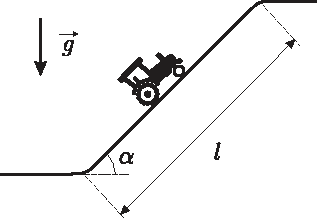
\includegraphics[width=0.5\linewidth]{2005-lahg-02-yl}
\end{center}
\fi
}

% Ü10
\ylDisplay{Keha} % Ülesande nimi
{Tundmatu autor} % Autor
{lahtine} % Voor
{2006} % Aasta
{G 3} % Ülesande nr.
{2} % Raskustase
{
% Teema: Dünaamika
\ifStatement
Vertikaalselt ülesse visatud keha läbib kaks korda kõrgusel $h$ asuvat punkti. Ajavahemik nende kahe läbimise vahel on $\Delta t$. Leida keha algkiirus $v_0$ ja aeg $\tau$ keha liikumise algusest kuni algpunkti tagasi jõudmiseni.
\fi
}

% Ü11
\ylDisplay{Mootorratas} % Ülesande nimi
{Tundmatu autor} % Autor
{lahtine} % Voor
{2007} % Aasta
{G 5} % Ülesande nr.
{2} % Raskustase
{
% Teema: Dünaamika
\ifStatement
Mootorrattur tahab hüpata üle kraavi, mille mõõtmed on näidatud joonisel. Kui suur peab olema mootorratturi minimaalne kiirus $v$ lennu alguses selleks, et tema ettevõtmine õnnestuks?

\begin{center}
	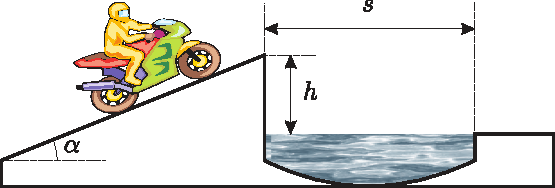
\includegraphics[width=0.8\linewidth]{2007-lahg-05-yl}
\end{center}
\fi
}

% Ü12
\ylDisplay{Kelk} % Ülesande nimi
{Tundmatu autor} % Autor
{lahtine} % Voor
{2008} % Aasta
{G 2} % Ülesande nr.
{2} % Raskustase
{
% Teema: Dünaamika
\ifStatement
\begin{wrapfigure}[5]{r}{0.4\textwidth}
	\begin{center}
		\vspace{-20pt}
		\hspace{-10pt}
		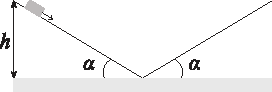
\includegraphics[width=\linewidth]{2008-lahg-02-yl}
	\end{center}
\end{wrapfigure}
Kelguga lastakse alla $h = \SI{10}{m}$ kõrgusest $\alpha = \SI{30}{\degree}$ kaldenurgaga orunõlvast. Kui kõrgele tõuseb kelk saadud hooga mööda sama suure kaldenurgaga vastasnõlva, kui hõõrdetegur on $\mu = \num{0,1}$? 

\emph{Märkus}. joonis on ligikaudne, languselt tõusule üleminek on tegelikult sujuv ja põrkega seotud kiirusekadu seal ei toimu.
\fi
}

% Ü13
\ylDisplay{Hantel} % Ülesande nimi
{Mihkel Kree} % Autor
{lõppvoor} % Voor
{2008} % Aasta
{G 1} % Ülesande nr.
{2} % Raskustase
{
% Teema: Dünaamika
\ifStatement
Hantel koosneb kahest võrdse massiga kerast (kumbki massiga $m$) ning neid ühendavast massitust jäigast vardast. Alguses hoitakse hantel horisontaalselt õhus paigal. Nüüd antakse ühele kuulidest hetkega vertikaalsuunaline kiirus $v$ ning hantel hakkab vabalt liikuma. Vabalangemise kiirendus on $g$. Missugune on süsteemi kineetiline energia hetkel, mil massikese saavutab maksimaalse kõrguse?
\fi
}

% Ü14
\ylDisplay{Ping-pong} % Ülesande nimi
{Siim Ainsaar} % Autor
{lõppvoor} % Voor
{2008} % Aasta
{G 2} % Ülesande nr.
{2} % Raskustase
{
% Teema: Dünaamika
\ifStatement
Pingpongipall kukutatakse kõrguselt $h$ horisontaalsele lauale. Igal põrkel kahaneb palli energia $k$ korda. Leidke palli lahtilaskmisest seismajäämiseni kuluv aeg $t$. Vabalangemise kiirendus on $g$.
\fi
}

% Ü15
\ylDisplay{Mürsk} % Ülesande nimi
{Mihkel Kree} % Autor
{piirkonnavoor} % Voor
{2009} % Aasta
{G 2} % Ülesande nr.
{2} % Raskustase
{
% Teema: Dünaamika
\ifStatement
Kahurist välja lennanud mürsk (massiga $M$) laguneb oma lennutrajektoori kõrgeimas punktis mingi sisemise vedrumehanismi abil kaheks võrdseks pooleks (kumbki massiga $M/2$) nii, et üks osadest kukub mürsu senist trajektoori pidi liikudes täpselt kahurini tagasi. Kui kaugele kahurist maandub teine pool? Lagunemispunkti projektsioon maapinnale asub kahurist kaugusel $L$.
\fi
}

% Ü16
\ylDisplay{Kerad} % Ülesande nimi
{Valter Kiisk} % Autor
{lahtine} % Voor
{2010} % Aasta
{G 1} % Ülesande nr.
{2} % Raskustase
{
% Teema: Dünaamika
\ifStatement
On antud kolm väliselt identset ja ühesuguse massiga kera. On teada, et üks
neist keradest on homogeenne, teine on seest õõnes ja kolmas on seest vedel.
Kuidas saab lihtsate võrdlevate mehaanikakatsetega kindlaks teha, milline on iga
kera sisemus? Abivahendid võite vabalt valida, aga kerasid vigastada ei tohi.
\fi
}

% Ü17
\ylDisplay{Sild} % Ülesande nimi
{Valter Kiisk} % Autor
{lõppvoor} % Voor
{2010} % Aasta
{G 1} % Ülesande nr.
{2} % Raskustase
{
% Teema: Dünaamika
\ifStatement
Risti üle $l=\SI{100}{m}$ laiuse jõe kulgeb kumer sild, mille keskel on
autotee $h=\SI{5}{m}$ võrra kõrgemal kaldapealsest tasemest. Silla profiiliks on
ringjoone kaar. Auto massiga $m=\SI{1000}{kg}$ ületab silla muutumatu kiirusega $v=\SI{60}{km/h}$.
Kui suure jõuga rõhub auto silla keskkohta? Kui suure kiiruse juures hakkab kaduma
kontakt rataste ja tee vahel?
\fi
}

% Ü18
\ylDisplay{Varras} % Ülesande nimi
{Stanislav Zavjalov} % Autor
{lõppvoor} % Voor
{2011} % Aasta
{G 2} % Ülesande nr.
{2} % Raskustase
{
% Teema: Dünaamika
\ifStatement
Mööda liigendi abil seina külge kinnitatud väga pikka ja tühiselt
kerget varrast saab libiseda väike rõngas massiga $m$. Esialgu asub rõngas liigendist kaugusel $l$ ja varras on horisontaalne. Ajahetkel $t = \num{0}$ hakkab süsteem
vabalt liikuma. Leidke varda ja horisontaali vahelise nurga $\alpha$ ajaline sõltuvus.
Kõik liikumised lugeda hõõrdevabaks. 
\fi
}

% Ü19
\ylDisplay{Kadunud rahakott} % Ülesande nimi
{Eero Vaher} % Autor
{lahtine} % Voor
{2012} % Aasta
{G 2} % Ülesanne nr.
{2} % Raskustase
{
% Teema: Dünaamika
\ifStatement
Suusahüppemäe hoovõturada asub nõlval, mille tõusunurk on $\alpha$. Hoovõturaja alumine
ots on horisontaalne. Suusahüppaja alustas hoovõttu kõrguselt $h$,
kuid kohe hoovõtu alguses kukkus tal rahakott taskust välja. Kui kaugele
äratõukepunktist (mööda
horisontaali) rahakott lendab, kui see liigub ilma takistuseta?
\fi
}

% Ü20
\ylDisplay{Kivi} % Ülesande nimi
{Taavi Pungas} % Autor
{lahtine} % Voor
{2013} % Aasta
{G 1} % Ülesande nr.
{2} % Raskustase
{
% Teema: Dünaamika
\ifStatement
Juku avastas maast välja turritamas poolkerakujulise kivi. Mõõtes mõõdulindiga
selle ümbermõõdu, sai ta tulemuseks $a=\SI{2,4}{m}$. Edasi võttis ta taskust tikutopsi ja
hakkas seda poolkera tipust alates natukesehaaval allapoole liigutama, kuni
lõpuks tikutops kivilt maha libises. Mõõdulindiga mööda poolkera mõõtes sai ta
tipu ja libisemispaiga vaheliseks kauguseks $b=\SI{20}{cm}$. Kui suur oli kivi
ja tikutopsi vaheline hõõrdetegur?
\fi
}

% Ü21
\ylDisplay{Kelgutaja} % Ülesande nimi
{Taavi Pungas} % Autor
{piirkonnavoor} % Voor
{2013} % Aasta
{G 4} % Ülesande nr.
{2} % Raskustase
{
% Teema: Dünaamika
\ifStatement
Lapsel kulus ühtlase kaldega nõlvast kõrgusega $h=\SI{2,0}{m}$ alla
kelgutamiseks $t=\SI{3,0}{s}$. kui suur vähemalt pidi sel juhul olema nõlva
kaldenurk~$\alpha$, kui ta alustas sõitu paigalseisust?
\fi
}

% Ü22
\ylDisplay{Pall} % Ülesande nimi
{Taivo Pungas} % Autor
{lõppvoor} % Voor
{2013} % Aasta
{G 2} % Ülesande nr.
{2} % Raskustase
{
% Teema: Dünaamika
\ifStatement
Madis analüüsis arvutiprogrammiga palli põrkamisest tehtud helilindistust
ja sai joonisel toodud graafiku, mis näitab helisignaali kuju.
Kui on teada, et pärast kolmandat põrget tõusis pall täpselt \SI{1}{m} kõrgusele,
leidke palli maksimaalne kõrgus pärast esimest põrget.
\begin{center}
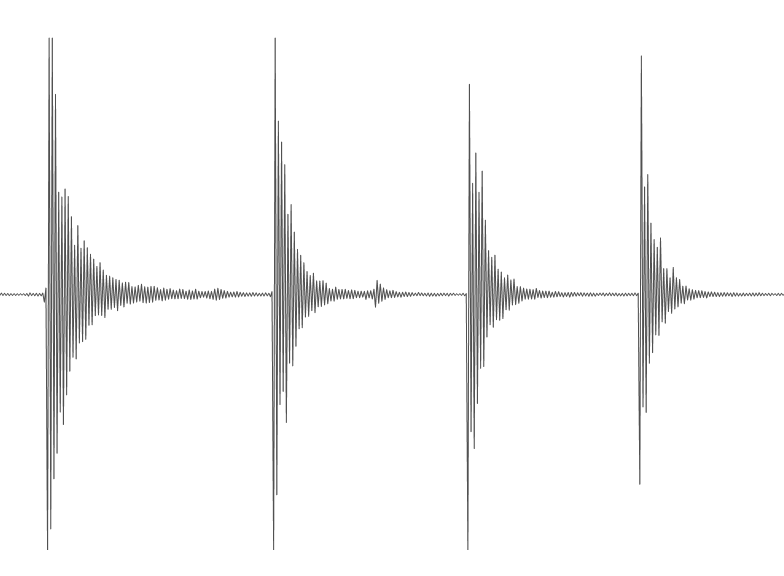
\includegraphics[width=0.5\textwidth]{2013-v3g-02-pall}%
\end{center}
\fi
}

% Ü23
\ylDisplay{Kaubarong} % Ülesande nimi
{Mihkel Rähn} % Autor
{lahtine} % Voor
{2014} % Aasta
{G 1} % Ülesande nr.
{2} % Raskustase
{
% Teema: Dünaamika
\ifStatement
Kaubarongi massiga $m=\SI{5000}{t}$ veab vedur võimsusega $N=\SI{2500}{kW}$. Veerehõõrdetegur rataste ja rööpa vahel on $\mu=\SI{0,002}{}$.\\
\osa Leidke rongi kiirus $v_1$ horisontaalsel teel.\\
\osa Leidke rongi kiirus $v_2$ tõusul üks sentimeeter ühe meetri kohta.\\
Õhutakistusega mitte arvestada.
\fi
}

% Ü24
\ylDisplay{Vaakumkahur} % Ülesande nimi
{Andreas Valdmann} % Autor
{lahtine} % Voor
{2014} % Aasta
{G 2} % Ülesande nr.
{2} % Raskustase
{
% Teema: Dünaamika
\ifStatement
Joonisel on kujutatud niinimetatud vaakumkahur. Laadimiseks pistetakse laskemoonaks olev pall vaakumkahuri toru vasakpoolsest otsast sisse. Seejärel kaetakse toru mõlemad otsad kergestirebeneva õhukindla membraaniga, näiteks fooliumiga, ning pumbatakse torust õhk välja. Nüüd on vaakumkahur laskevalmis. Tulistamiseks purustatakse vasakpoolne membraan, mille tagajärjel hakkab pall toru parempoolse otsa poole sööstma. Piisavalt pika toru korral purustab pall parempoolse membraani ning lendab torust välja. Olgu palli läbimõõt võrdne toru siseläbimõõduga $d=\SI{4,0}{cm}$, palli mass $m=\SI{24}{g}$ ja asugu pall enne tulistamist $l=\SI{150}{cm}$ kaugusel toru parempoolsest otsast. Kui suur on palli kiirus vahetult enne parempoolse membraani läbimist? Õhurõhk on $P_0=\SI{100}{kPa}$. Hõõrdumisega pole tarvis arvestada.
\begin{center}
 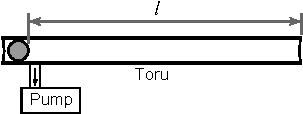
\includegraphics[width=0.75\textwidth]{2014-lahg-02-vaakumkahur.pdf}
\end{center}
\fi
}

% Ü25
\ylDisplay{Mängukahur} % Ülesande nimi
{EFO žürii} % Autor
{lahtine} % Voor
{2016} % Aasta
{G 1} % Ülesande nr.
{2} % Raskustase
{
% Teema: Dünaamika
\ifStatement
\begin{wrapfigure}[6]{r}{0.4\textwidth}
 \vspace{-20pt}
 \begin{center}
 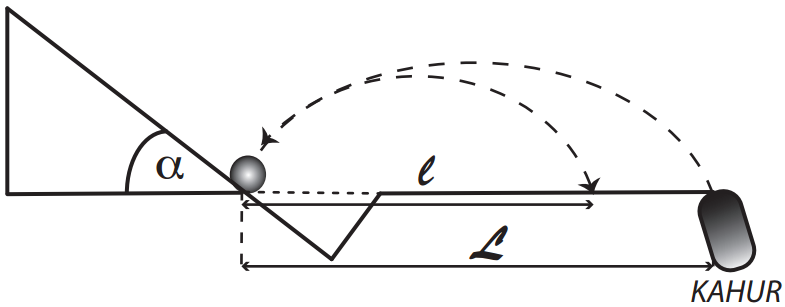
\includegraphics[width=0.4\textwidth]{2016-lahg-01-kaldjoonis}
 \end{center}
 \vspace{-30pt}
\end{wrapfigure}

Mängukahurist tulistatakse kummipall nii, et see põrkab risti kaldpinnaga, kahurist horisontaalkaugusel $L$. Pall põrkab kaldpinnast tagasi kaugusele $l$ (vt joonis). Leidke, kui suur osa energiast neeldus põrkel. Kaldpinna kaldenurk on $\alpha$.
\fi
}

% Ü26
\ylDisplay{Köievedu} % Ülesande nimi
{Oleg Košik} % Autor
{piirkonnavoor} % Voor
{2016} % Aasta
{G 2} % Ülesande nr.
{2} % Raskustase
{
% Teema: Dünaamika
\ifStatement
Eero ja Oleg võistlevad köieveos nii, et kogu võistluse ajal on köis horisontaalne. Eero mass $m_1=\SI{110}{kg}$ ja Olegi mass $m_2=\SI{85}{kg}$. Hõõrdetegur talla ja põranda vahel $\mu=\SI{0,30}{}$ on mõlemal mehel sama. Kumb mees võidab? Millise maksimaalse kiirendusega saab võitja sundida kaotajat liikuma, nii et ta ise veel paigale jääks? Raskuskiirendus $g=\SI{9,8}{m/s^2}$.
\fi
}

% Ü27
\ylDisplay{Vastlaliug} % Ülesande nimi
{Moorits Mihkel Muru} % Autor
{lõppvoor} % Voor
{2017} % Aasta
{G 1} % Ülesande nr.
{2} % Raskustase
{
% Teema: Dünaamika
\ifStatement
\begin{wrapfigure}[5]{r}{0.45\linewidth}
	\vspace{-5pt}
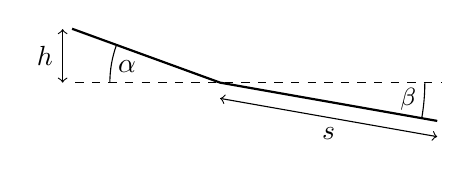
\begin{tikzpicture}[scale=0.4]
% Nõlv
\draw [thick] (0,0) -- (160:5);
\draw [thick] (0,0) -- (-10:7);

% Nurgad
\draw [dashed] (-4.6,0) -- (7,0);
\draw (160:3.5) arc (160:180:3.5) node at (170:3) {\(\alpha\)};
\draw (0:6.5) arc (0:-10:6.5) node at (-5:6) {\small\(\beta\)};

% Suurused
\draw [<->] (-5,0) -- (-5,1.7) node[pos=0.5, left] {\(h\)};
\draw [<->, yshift=-0.5cm] (0,0) -- (-10:7) node[pos=0.5, below] {\(s\)};	
\end{tikzpicture}
%\caption{Künka läbilõige} \label{liug}
\end{wrapfigure}

Juss leidis vastlaliu laskmiseks künka, mille läbilõige koosneb kahest sirglõigust, nagu näha joonisel, edasi on horisontaalne maa. Esimese nõlvaosa kõrgus on \(h=\SI{2}{\meter}\) ja selle kalle \(\alpha=\ang{20}\), teise osa pikkus on \(s=\SI{20}{\meter}\) ja kalle \(\beta=\ang{5}\). Jussi mass koos kelguga on \(m=\SI{47}{\kilogram}\) ja hõõrdetegur lume ja kelgu vahel on \(\mu=\num{0.08}\), raskuskiirendus \(g=\SI{9.8}{\meter\per\second\squared}\). Leidke, kui pikk on Jussi vastlaliug.
\fi
}

% Ü28
\ylDisplay{Karatist} % Ülesande nimi
{Tundmatu autor} % Autor
{lahtine} % Voor
{2007} % Aasta
{G 6} % Ülesande nr.
{3} % Raskustase
{
% Teema: Dünaamika
\ifStatement
Hinnake, millise kiirusega $v$ peab karatisti käsi tabama kahele kivile toetuva lauajupi keskpunkti (vt joonist), et laud murduks? Käe mass on $m = \SI{1,5}{kg}$, laua mass $M = \SI{2}{kg}$, laua jäikustegur $k = \SI{1,4e5}{N/m}$, murdumiseks vajalik läbipaine (st laua keskpunkti nihe) $d = \SI{20}{mm}$. 

\emph{Märkus}. Jäikustegur $k$ on võrdetegur laua keskpunkti rakendatud jõu $F$ ning laua keskpunkti nihke $x$ vahel (vt joonist).

\begin{center}
	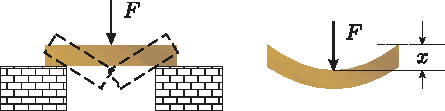
\includegraphics[width=0.8\linewidth]{2007-lahg-06-yl}
\end{center}
\fi
}

% Ü29
\ylDisplay{Veenus} % Ülesande nimi
{Mihkel Kree} % Autor
{lõppvoor} % Voor
{2007} % Aasta
{G 2} % Ülesande nr.
{3} % Raskustase
{
% Teema: Dünaamika
\ifStatement
Lugegem Maa ja Veenuse orbiidid ümber Päikese ringikujulisteks. Planeedid tiirlevad ümber Päikese samas suunas ja Veenuse maksimaalne eemaldumus (nurk Veenuse ja Päikese vahel Maalt vaadates) on 46 kraadi.\\
\osa Leidke Veenuse ja Maa orbiitide raadiuste suhe.\\
\osa Mitu päeva jääb järjestikuste maksimaalsete eemaldumuste vahele?

\emph{Vihje}. Kepleri seaduse kohaselt on taevakehade tiirlemisperioodide ruudud võrdelised vastavate orbiitide raadiuste kuupidega.
\fi
}

% Ü30
\ylDisplay{Auto} % Ülesande nimi
{Mihkel Heidelberg} % Autor
{piirkonnavoor} % Voor
{2009} % Aasta
{G 5} % Ülesande nr.
{3} % Raskustase
{
% Teema: Dünaamika
\ifStatement
Auto kiirendab nii, et rattad libisevad. Hetkel on auto kiirus stabiilselt $v$, vedavate rataste nurkkiirus $\omega$ ja raadius $r$. Kui oletada, et mootori võimsus läheb ainult auto liikumisse ja vedavate rataste libisemisse, siis kui suur on kasutegur?
\fi
}

% Ü31
\ylDisplay{Vedru} % Ülesande nimi
{Aigar Vaigu} % Autor
{piirkonnavoor} % Voor
{2010} % Aasta
{G 4} % Ülesande nr.
{3} % Raskustase
{
% Teema: Dünaamika
\ifStatement
Raske tellis kukub poole meetri kõrguselt jäigale lühikesele vedrule. Põrge
on elastne ja tellis lendab peaaegu algsele kõrgusele tagasi. Kui
kõrgele maast kerkib vedru pärast põrget?
\fi
}

% Ü32
\ylDisplay{Pendel} % Ülesande nimi
{Taavi Pungas} % Autor
{piirkonnavoor} % Voor
{2011} % Aasta
{G 7} % Ülesande nr.
{3} % Raskustase
{
% Teema: Dünaamika
\ifStatement
Pendel pandi väikese amplituudiga võnkuma ning stopperiga registreeriti neid hetki, kui pendel läbis vasakult poolt tulles oma tasakaalupunkti. Kaks järjestikust sellist sündmust toimusid hetkedel $t_1=\SI{3,19}{s}$ ja $t_2=\SI{5,64}{s}$. Pendlil lasti mõnda aega segamatult võnkuda, seejärel saadi kaheks järjestikuseks näiduks $t_3=\SI{61,14}{s}$ ja $t_4=\SI{63,54}{s}$. Leidke võimalikult täpselt pendli võnkeperiood ning hinnake selle mõõtemääramatust.
\fi
}

% Ü33
\ylDisplay{Alpinist} % Ülesande nimi
{Kaur Aare Saar} % Autor
{lahtine} % Voor
{2013} % Aasta
{G 3} % Ülesande nr.
{3} % Raskustase
{
% Teema: Dünaamika
\ifStatement
Alpinist massiga $m=\SI{75}{kg}$ on kinnitatud elastse nööri külge pikkusega
$L=\SI{6}{m}$. Nööri teine ots on kinnitatud kalju külge. Olles roninud 6 meetri
kõrgusele kinnituskohast, ta kukub. Leidke, kui suur võib olla ülimalt nööri
elastsustegur $k$, teades, et suurim nööri tõmbejõud, mida inimene talub, on
$T=25mg$. Õhutakistust ärge arvestage.
\fi
}

% Ü34
\ylDisplay{Langevarjuhüpe} % Ülesande nimi
{Taavi Pungas} % Autor
{piirkonnavoor} % Voor
{2014} % Aasta
{G 5} % Ülesande nr.
{3} % Raskustase
{
% Teema: Dünaamika
\ifStatement
Juku massiga $m=\SI{60}{\kg}$ ja tema isa Juhan massiga $M=\SI{90}{\kg}$ otsustasid teha langevarjuhüppe. Neile pandi selga ühesugused langevarjud massiga $m_v=\SI{10}{\kg}$ ning nad lükati lennukist välja. Mõlema langevarjud avanesid täielikult ühesugusel kõrgusel $h$, pärast mida saavutasid hüppajad tühise aja jooksul konstantse kiiruse ja liuglesid sellel kiirusel maapinnani. Jukul kulus langevarju avanemisest maapinnani jõudmiseks aega $t=\SI{110}{\s}$. Kui pikk aeg $T$ kulus selleks Juhanil? Langevarjule õhu poolt mõjuv takistusjõud on võrdeline langemiskiiruse ruuduga. Lihtsuse mõttes loeme hüppajatele endile mõjuva õhutakistuse tühiselt väikeseks.
\fi
}

% Ü35
\ylDisplay{Kelk} % Ülesande nimi
{Joonas Kalda} % Autor
{piirkonnavoor} % Voor
{2016} % Aasta
{G 4} % Ülesande nr.
{3} % Raskustase
{
% Teema: Dünaamika
\ifStatement
\begin{wrapfigure}[2]{r}{0.3\textwidth}
	\vspace{-12pt}
	\begin{resizebox}{\linewidth}{!}{
	\begin{tikzpicture}
	\coordinate (C) at (0.7,-0.1);
	\draw (0,0) -- ++(180-15:1.5);
	\draw (0,0) to [out = -15, in = 180] (C);
	\draw (C) to ++(0:1.5);
	\draw (180-15:1.5) -- ++(-15:0.2) -- ++(90-15:0.1) -- ++(180-15:0.2) -- (180-15:1.5);
	\end{tikzpicture}}
	\end{resizebox}
\end{wrapfigure}

Juku tahab kelguga ületada jääga kaetud jõge. Ta stardib lumega kaetud kaldalt, mis on horisondiga $\alpha = 15^{\circ}$ nurga all. Jõe laius $l = \SI{10}{m}$, kelgu ja lume vaheline hõõrdetegur $\mu_1 = \SI{0.20}{}$, kelgu ja jää vaheline hõõrdetegur $\mu_2 = \SI{0.10}{}$. Kui kõrgele veepinnast peab kallas ulatuma, et Juku libiseks teise kaldani?
\fi
}

% Ü36
\ylDisplay{Pidurdus} % Ülesande nimi
{Eero Vaher} % Autor
{lõppvoor} % Voor
{2016} % Aasta
{G 2} % Ülesande nr.
{3} % Raskustase
{
% Teema: Dünaamika
\ifStatement
Auto sõidab teel, mille kõrguse muut teepikkuse kohta on $k=\frac{1}{30}$. Ühesuguse algkiiruse ning pidurdusjõu korral jääb auto ülesmäge liikudes seisma vahemaa $s_1=\SI{25}{m}$ jooksul, allamäge liikudes aga vahemaa $s_2=\SI{30}{m}$ jooksul. Mis on auto algkiiruse $v$ väärtus? Raskuskiirendus $g=\SI{9.8}{\meter\per\second\squared}$.
\fi
}

% Ü37
\ylDisplay{Kahurikuul} % Ülesande nimi
{Hans Daniel Kaimre} % Autor
{lõppvoor} % Voor
{2016} % Aasta
{G 3} % Ülesande nr.
{3} % Raskustase
{
% Teema: Dünaamika
\ifStatement
Juku arvutas koolitunnis ülivõimsast kahurist otse üles lastud kuuli maksimaalseks kõrguseks $H=\SI{400}{\km}$. Ta ei arvestanud aga seda, et sellistel kõrgustel gravitatsioonivälja muutus on juba märkimisväärne ning ei saa eeldada, et raskusjõud on konstantne. Leidke, kui kõrgele kuul tegelikult lendaks. Maa raadius $R=\SI{6400}{\km}$. Õhutakistusega mitte arvestada.
\fi
}

% Ü38
\ylDisplay{Pendel} % Ülesande nimi
{Andreas Valdmann} % Autor
{piirkonnavoor} % Voor
{2017} % Aasta
{G 3} % Ülesande nr.
{3} % Raskustase
{
% Teema: Dünaamika
\ifStatement
Nöörist ja koormisest koosnev pendel võngub nii, et amplituudasendis on nööri ja vertikaalsihi vaheline nurk $\alpha=\SI{60}{\degree}$. Mitu korda erinevad võnkumise käigus suurim ja vähim pinge nööris?
\fi
}

% Ü39
\ylDisplay{Mäenõlv} % Ülesande nimi
{Jonatan Kalmus} % Autor
{lõppvoor} % Voor
{2017} % Aasta
{G 2} % Ülesande nr.
{3} % Raskustase
{
% Teema: Dünaamika
\ifStatement
Kui suure maksimaalse kaldenurgaga $\alpha$ mäenõlvast on võimalik jalgrattaga konstantse kiirusega üles sõita? Ratturi mass on $m$, jalgratta mass $M$, pedaali vända pikkus $r_1$, eesmise hammasratta raadius $r_2$, tagumise hammasratta raadius $r_3$, ratta raadius $r_4$. Eeldada, et ratturi massikese püsib sõitmise käigus ratta suhtes paigal ja sõitja kannab kogu oma kehakaalu vajuval pedaalil. Hõõrdetegur pinna ja ratta vahel on piisavalt suur libisemise vältimiseks. Mehaanilise hõõrdumisega jõuülekandes mitte arvestada ning veerehõõrdejõu võib lugeda tühiseks. Eeldada, et jalgratta keskmine kiirus püsib ligikaudselt konstante ja kiiruse suhteline muutus veerand väntamisperioodi jooksul on tühiselt väike.\\
\emph{Märkus.} Ülesande teksti on olümpiaadil esineva versiooniga võrreldes kohandatud.
\fi
}

% Ü40
\ylDisplay{Aerud} % Ülesande nimi
{Tundmatu autor} % Autor
{piirkonnavoor} % Voor
{2005} % Aasta
{G 6} % Ülesande nr.
{4} % Raskustase
{
% Teema: Dünaamika
\ifStatement
Aerude pikkus tullist (punktist, kus aerud kinnituvad paadi kere külge) kuni käepidemeni on $a = \SI{1}{m}$ ning tullist kuni labadeni on $b = \SI{1,5}{m}$. Keskmine jõud, millega aerutaja tõmbab kumbagi aeru, on $F = \SI{60}{N}$. Paadi ja vee vaheline takistusjõud on $F_h = \alpha v^2$, kus $\alpha = \SI{20}{kg/m}$. Kui suure keskmise kiirusega liigub paat? Hinnata aerutaja keskmist võimsust.
\fi
}

% Ü41
\ylDisplay{Kivi} % Ülesande nimi
{Tundmatu autor} % Autor
{lahtine} % Voor
{2006} % Aasta
{G 4} % Ülesande nr.
{4} % Raskustase
{
% Teema: Dünaamika
\ifStatement
Paelaga lae külge kinnitatud kivi liigub mööda horisontaaltasapinnas asuvat ringjoont, mille kaugus laest $h = \SI{1,25}{m}$. Leida kivi tiirlemisperiood $\tau$. 
\fi
}

% Ü42
\ylDisplay{Kaldpind} % Ülesande nimi
{Mihkel Rähn} % Autor
{piirkonnavoor} % Voor
{2006} % Aasta
{G 4} % Ülesande nr.
{4} % Raskustase
{
% Teema: Dünaamika
\ifStatement
Pall kukub kaldpinnale ja hakkab elastselt põrkuma (st energiakadudeta). Kui kaugel on viies põrkekoht esimesest? Kaldpinna kaldenurk on $\alpha$, palli algkõrgus esimesest põrkekohast oli $h$.
\fi
}

% Ü43
\ylDisplay{Kuulike} % Ülesande nimi
{Tundmatu autor} % Autor
{lahtine} % Voor
{2008} % Aasta
{G 5} % Ülesande nr.
{4} % Raskustase
{
% Teema: Dünaamika
\ifStatement
Venimatu ja kaalutu niidi otsa kinnitati kuulike.
Niit viidi horisontaalasendisse ja lasti lahti. Kuulikese kiiruse vertikaalne komponent
hakkab esialgu suurenema, kuid teatud hetkest alates vähenema. Millise nurga moodustab niit vertikaalsihiga ajahetkel, kui kuulikese kiiruse vertikaalne komponent on
maksimaalne?
\fi
}

% Ü44
\ylDisplay{Veerev silinder} % Ülesande nimi
{Andres Laan} % Autor
{lahtine} % Voor
{2010} % Aasta
{G 3} % Ülesande nr.
{4} % Raskustase
{
% Teema: Dünaamika
\ifStatement
\begin{wrapfigure}[7]{r}{0.3\textwidth}
	\vspace{-10pt}
	\hspace{-8pt}
	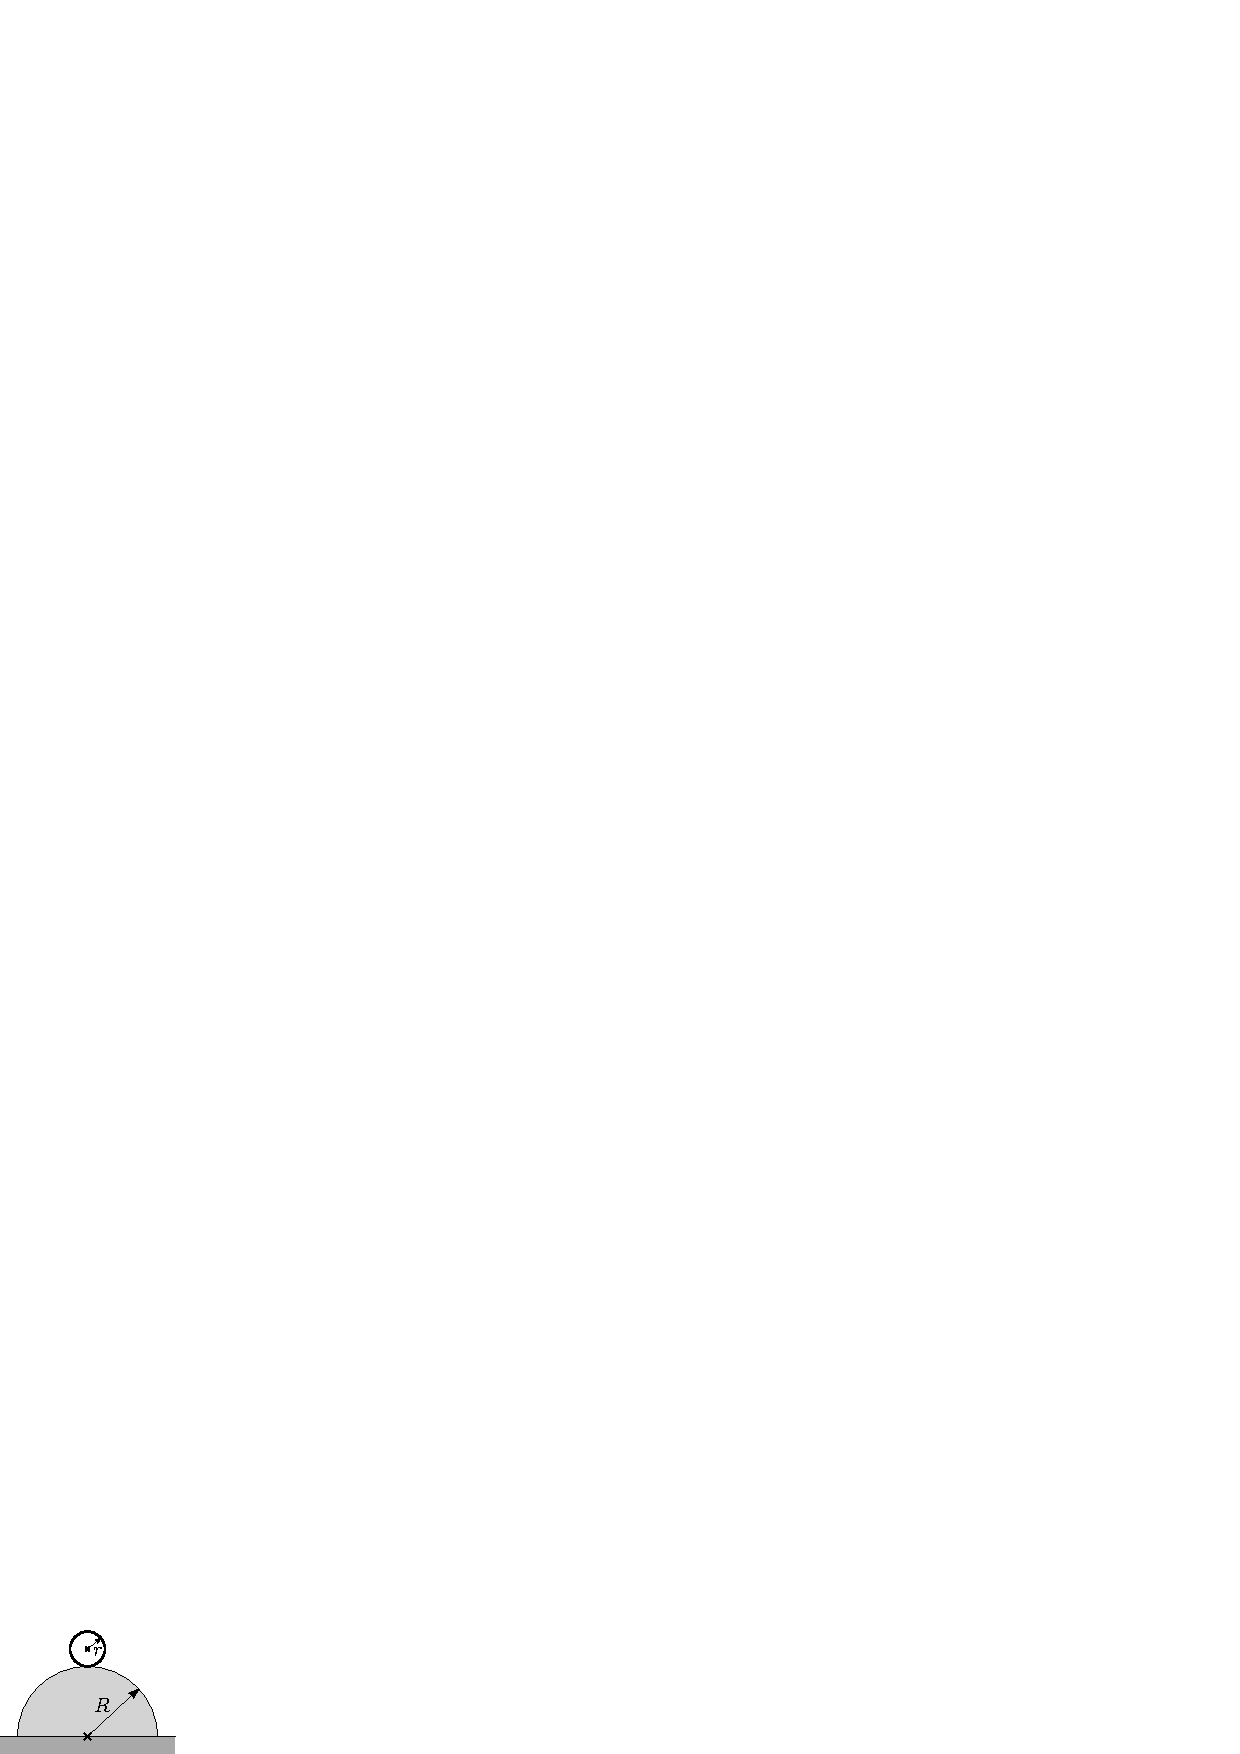
\includegraphics[width=\linewidth]{2010-lahg-03-silindri_joonis_ipe}
\end{wrapfigure}

Alusele kinnitatud poolsilindril raadiusega $R$
lebab selle kõrgeimas punktis seest tühi silinder
raadiusega $r$. Mingisugusel hetkel nihkub keha natuke tasakaalust välja ja
selle tulemusel hakkab libisemiseta veerema (hõõrdetegur on väga suur). Leidke, kui kõrgel aluse kohal keha
poolsilindri pinnast eraldub. \emph{Vihje:} kui veereva silindri mass on $m$ ja
ta masskese liigub kiirusega $v$, on ta kineetiline energia $m v^2$ (ilma
kordajata $\frac12$!).
\fi
}

% Ü45
\ylDisplay{Veoauto} % Ülesande nimi
{Kristian Kuppart} % Autor
{lahtine} % Voor
{2011} % Aasta
{G 3} % Ülesande nr.
{4} % Raskustase
{
% Teema: Dünaamika
\ifStatement
Veoauto kastis kõrgusega $H$ on vedelik, mille pinna kõrgus kasti põhjast on 
$h$, kusjuures $h > \frac{H}{2}$. Kui suure kiirendusega $a$ saab veoauto 
liikuda, ilma et vedelik kastist välja voolaks? Veoauto kasti pikkus on $L$.\\
\textit{Märkus.} Auto kiirendab sujuvalt ning tänu sellele vedelik võnkuma ei hakka.
\fi
}

% Ü46
\ylDisplay{Surmasõlm} % Ülesande nimi
{Andreas Valdmann} % Autor
{piirkonnavoor} % Voor
{2012} % Aasta
{G 5} % Ülesande nr.
{4} % Raskustase
{
% Teema: Dünaamika
\ifStatement
\begin{wrapfigure}{r}{42mm}%
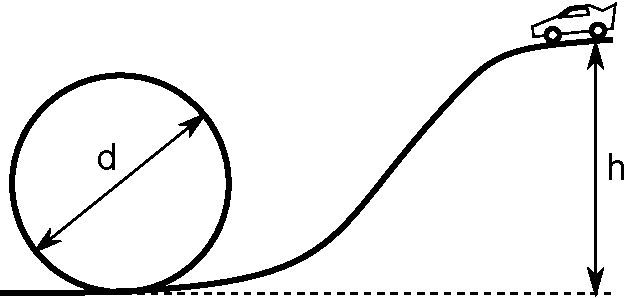
\includegraphics[width=\linewidth]{2012-v2g-05-silmus}%
\end{wrapfigure}
Mudelauto rada on kujutatud joonisel: auto alustab kaldtee tipus seisvast
asendist, kogub laskumisel kiirust ja teeb silmuses surmasõlme. Mis on
minimaalne kõrgus $h$, et auto silmuse läbimisel alla ei kukuks? Silmuse
läbimõõt on $d$. Hõõrdumisega arvestada ei ole vaja.
\fi
}

% Ü47
\ylDisplay{Veejuga} % Ülesande nimi
{Mihkel Kree} % Autor
{lõppvoor} % Voor
{2012} % Aasta
{G 2} % Ülesande nr.
{4} % Raskustase
{
% Teema: Dünaamika
\ifStatement
Pildil on foto horisontaalsest torust väljuva veejoaga ning teljestik, mille
väikseim jaotis on võrdne veejoa läbimõõduga selle algkõrgusel. Ühtlase
kiirusega voolava veejoa alla pandud mõõteklaas ruumalaga
$V=\SI{150}{cm^3}$ täitus ajaga $t=\SI{5}{min}$. Leidke
toru siseläbimõõt.
\begin{center}
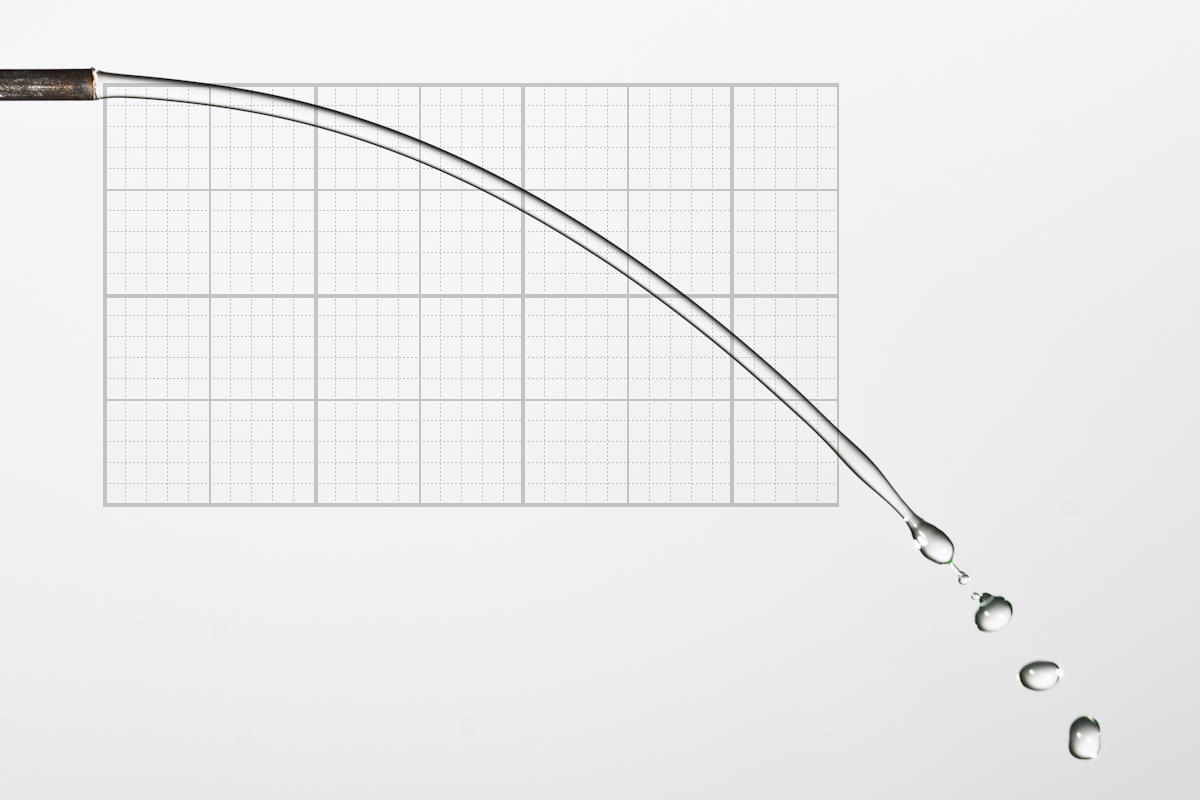
\includegraphics[width=0.7\linewidth]{2012-v3g-02-jet}%
\end{center}
\fi
}

% Ü48
\ylDisplay{Lasketiir} % Ülesande nimi
{Aigar Vaigu} % Autor
{piirkonnavoor} % Voor
{2016} % Aasta
{G 6} % Ülesande nr.
{4} % Raskustase
{
% Teema: Dünaamika
\ifStatement
Siselasketiirus tulistatakse vintpüssist, mille kuuli kiirus $v=\SI{320}{m/s}$, kaugusel $s=\SI{30}{m}$ olevat märklauda. Laskur sihib püssiga samal kõrgusel olevat märki ja tabab seda otse kümnesse. Hinnake, kui kaugele sihtmärgist satuks kuul, kui relva enne laskmist keerata ümber sihtimistelje 180 kraadi? Õhutakistusega mitte arvestada.
\fi
}

% Ü49
\ylDisplay{Silinder} % Ülesande nimi
{Kaur Aare Saar} % Autor
{lõppvoor} % Voor
{2016} % Aasta
{G 4} % Ülesande nr.
{4} % Raskustase
{
% Teema: Dünaamika
\ifStatement
Silinder massiga $m$ ja raadiusega $R$ libiseb tasapinnal kiirusega $v$ ja nurkkiirusega $\omega$. Kui libisemine on lõppenud, liigub silinder kiirusega $v$ esialgsega vastupidises suunas. Leidke silindri esialgne nurkkiirus.

\begin{center}
	\begin{resizebox}{0.35\linewidth}{!}{
			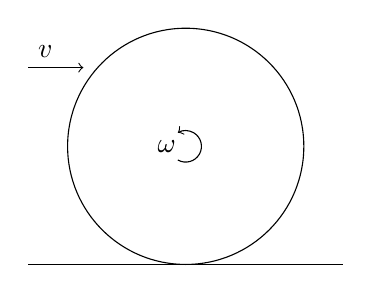
\begin{tikzpicture}
			\draw (0,2.5) node[anchor=south west] {$v$};
			\draw[->] (0,2.5) -- ++(0:0.7);
			\draw (0,0) --(4,0);
			\draw (2,1.5) circle (1.5);
			\draw [->] (2,1.5) node[anchor = east] {$\omega$} ++(-120:0.2) arc (-120:120:0.2);
			\end{tikzpicture}}
	\end{resizebox}
\end{center}
\fi
}

% Ü50
\ylDisplay{Veok ringteel} % Ülesande nimi
{Jonatan Kalmus} % Autor
{piirkonnavoor} % Voor
{2018} % Aasta
{G 5} % Ülesande nr.
{4} % Raskustase
{
% Teema: Dünaamika
\ifStatement
Veok sõidab ringteel kõverusraadiusega $R$ ühtlase kiirusega. Leida veoki maksimaalne võimalik kiirus, eeldusel et hõõrdetegur on piisavalt suur libisemise vältimiseks. Veoki massikeskme kõrgus maapinnast on $h$ ja veoki laius $l$. Raskuskiirendus on $g$.
\fi
}

% Ü51
\ylDisplay{Sfäär} % Ülesande nimi
{Andre Sääsk} % Autor
{lahtine} % Voor
{2005} % Aasta
{G 6} % Ülesande nr.
{5} % Raskustase
{
% Teema: Dünaamika
\ifStatement
Üks osa Pariisi Cité des Sciences teadusmuuseumi kompleksist --- La Géode --- kujutab endast hiigelsuurt sfääri raadiusega $R = \SI{18}{m}$, mille sees asub maailma suurim kinoekraan (vt joonist). Hoonet väljastpoolt imetlev uudishimulik koolipoiss otsustab tabada selle hoone tipp-punkti tennisepalliga. Kui suure minimaalse kiirusega $v$ peaks ta palli viskama, et palli liikumise trajektoor lõikuks hoone välispinnaga vaid ühes punktis --- hoone tipp-punktis --- ja see oleks ühtlasi ka palli liikumise trajektoori kõrgeimaks punktiks? Pall alustab liikumist kõrgusel $h = \SI{1,5}{m}$.

\begin{center}
	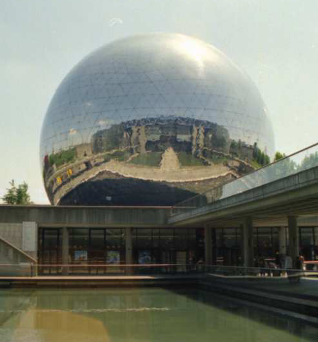
\includegraphics[width=0.5\linewidth]{2005-lahg-06-yl}
\end{center}
\fi
}

% Ü52
\ylDisplay{Anum} % Ülesande nimi
{Tundmatu autor} % Autor
{lahtine} % Voor
{2005} % Aasta
{G 7} % Ülesande nr.
{5} % Raskustase
{
% Teema: Dünaamika
\ifStatement
Siledal pinnal asub kerge ristkülikuline anum, mis on täidetud vedelikuga tihedusega $\rho_0$, vedeliku ruumala on $V_0$. Anuma põhja sattunud põrnikas ruumalaga $V$ ja tihedusega $\rho$ hakkab anuma põhja suhtes roomama kiirusega $u$. Millise kiirusega hakkab anum pinnal liikuma? Anuma mass on tühine, veetase jääb kogu aeg horisontaalseks. Eeldada, et pinna ja anuma vahel hõõre puudub.
\fi
}

% Ü53
\ylDisplay{Mullitaja} % Ülesande nimi
{Jaak Kikas} % Autor
{lõppvoor} % Voor
{2005} % Aasta
{G 7} % Ülesande nr.
{5} % Raskustase
{
% Teema: Dünaamika
\ifStatement
Veekogu põhjas asub mullitaja --- õhuballoon väikese avausega, millest võrdsete ajavahemike $\Delta t = \SI{1}{s}$ järel väljuvad õhumullid raadiusega $R = \SI{0,3}{mm}$. Taolise mullikese liikumisel vees mõjub sellele takistusjõud $F = 6\pi \eta Rv$, kus $\eta$ on vedeliku voolamistakistust iseloomustav tegur (vedeliku viskoossus, vee korral on selle suuruse väärtuseks \SI{1e-3}{N.s/m^2} ) ja $v$ on mullikese kiirus. Võite lugeda, et mullikese liikumine toimub kogu aeg kiirusega, mis on määratud tingimusega, et kõigi talle mõjuvate jõudude resultant on null. Vee tihedus $\rho = \SI{1000}{kg/m^3}$, raskuskiirendus $g = \SI{9,8}{m/s^2}$, õhurõhk $p_0 = \SI{100}{kPa}$. Mitu korda muutub vahemaa naabermullikeste vahel tõusul põhjast pinnale, kui veekogu sügavus on $H = \SI{27}{m}$?
\fi
}

% Ü54
\ylDisplay{Plokk} % Ülesande nimi
{Tundmatu autor} % Autor
{lahtine} % Voor
{2006} % Aasta
{G 5} % Ülesande nr.
{5} % Raskustase
{
% Teema: Dünaamika
\ifStatement
Kui suure kiirendusega $a_k$ ja mis suunas hakkab liikuma kahest kehast koosneva süsteemi masskese, kui kehad on seotud niidiga, mis on tõmmatud üle ploki (vt joonist)? Kehade massid on $m_1$ ja $m_2$ ($m_1$ < $m_2$), niit on kaalutu ja mitteelastne.
\begin{center}
	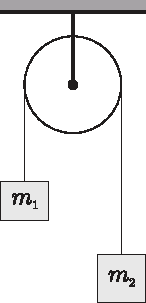
\includegraphics[width=0.25\linewidth]{2006-lahg-05-yl}
\end{center}
\fi
}

% Ü55
\ylDisplay{Kada} % Ülesande nimi
{Oleg Košik} % Autor
{lõppvoor} % Voor
{2006} % Aasta
{G 3} % Ülesande nr.
{5} % Raskustase
{
% Teema: Dünaamika
\ifStatement
Vaatame lihtsa kada ehk ragulka konstruktsiooni. Elastne kummipael tõmmatakse kahe fikseeritud otspunkti vahele, laskmiseks asetatakse kivi paela keskele, pael tõmmatakse koos kiviga pingule ja lastakse vabaks. Kivi lastakse lendu horisontaaltasandi suhtes nurga $\alpha = \SI{10}{\degree}$ all. Leidke, kui kaugele peab laskja tõmbama kivi, et tabada märki, mis asub kadast $L = \SI{25}{m}$ kaugusel ning sellega samal kõrgusel. Kui suurt jõudu peab ta selleks paelale rakendama? Kummipaela pikkus pingestamata olekus on $l = \SI{60}{cm}$, mis on ühtlasi ka paela kinnituspunktide vahekaugus. Pael lugeda kaalutuks ning jäikusteguriga $k = \SI{50}{N/m}$. Kivi mass on $m = \SI{20}{g}$. Õhutakistusega ei ole vaja arvestada. Raskusjõu mõju kivi kiirendamisel kadas pole vaja arvestada. Raskuskiirendus on $g = \SI{9.81}{m/s^2}$.
\fi
}

% Ü56
\ylDisplay{Hooratas} % Ülesande nimi
{Valter Kiisk} % Autor
{lõppvoor} % Voor
{2007} % Aasta
{G 4} % Ülesande nr.
{5} % Raskustase
{
% Teema: Dünaamika
\ifStatement
Hooratas raadiusega $R$ pöörleb nurkkiirusega $\omega$. Lihtsuse huvides võib hooratast vaadelda peenikese rõngana (pöörlemistelg ühtib rõnga teljega).\\
\osa Milline on energia salvestustihedus $w$ (kineetiline energia massiühiku kohta) hoorattas?\\
\osa Hooratas on valmistatud süsinikkiuga armeeritud polümeerist, mille tõmbetugevus $\sigma\idx{max} = \SI{2,4e9}{Pa}$ ja tihedus $\rho = \SI{1500}{kg/m^3}$. Hinnake energia salvestustiheduse maksimaalselt võimalikku väärtust sellises hoorattas (andes numbrilise vastuse).

\emph{Vihje}. Tõmbetugevus on maksimaalne jõud ristlõike pindala kohta, mida antud materjal talub ilma purunemata.
\fi
}

% Ü57
\ylDisplay{Maaler} % Ülesande nimi
{Valter Kiisk} % Autor
{lahtine} % Voor
{2010} % Aasta
{G 5} % Ülesande nr.
{5} % Raskustase
{
% Teema: Dünaamika
\ifStatement
Maaler on seina ülemise osa värvimiseks roninud kõrge, peaaegu vertikaalse
redeli tippu. Ettevaatamatu liigutuse tulemusena hakkab redel kukkuma ümber. Kas
vähemohtlik oleks redelist kohe lahti lasta või pigem klammerduda redeli külge?
Põrand on lai ja tühi, nii et (redeli) kukkumist ei takista miski. Redeli alumine
ots ei libise.
\emph{Vihje.} homogeensel vardal pikkusega $l$ ja massiga $m$ on ümber otsa
nurkkiirusega $\omega$ pööreldes kineetiline energia $\frac{m l^2 \omega^2}{6}$.
\fi
}

% Ü58
\ylDisplay{Benji-hüpe} % Ülesande nimi
{Andreas Valdmann} % Autor
{piirkonnavoor} % Voor
{2010} % Aasta
{G 6} % Ülesande nr.
{5} % Raskustase
{
% Teema: Dünaamika
\ifStatement
Benji-hüppaja massiga $m=\SI{80}{kg}$ kasutab köit pikkusega $l=\SI{35}{m}$, mille jäikustegur $k=\SI{60}{N/m}$. Kui kõrgele maapinnast tuleks tõsta hüppeplatvorm, et jääks ohutusvaru $h=\SI{5}{m}$? Mis on suurim kiirus, mille hüppaja saavutab? Raskuskiirendus $g=\SI{9.8}{m/s^2}$. Hüppaja mõõtmetega arvestama ei pea. 
\fi
}

% Ü59
\ylDisplay{Kloori molekul} % Ülesande nimi
{Ants Remm} % Autor
{lahtine} % Voor
{2012} % Aasta
{G 6} % Ülesande nr.
{5} % Raskustase
{
% Teema: Dünaamika
\ifStatement
Kloori molekul, mis liigub kiirusega $v = \SI{600}{m/s}$, neelab
footoni lainepikkusega $\lambda = \SI{350}{nm}$ ning jaguneb kaheks aatomiks.
Ühe aatomi kiiruseks
mõõdetakse $ u = \SI{1600}{m/s}$, mis on risti molekuli esialgse
kiirusega. Leidke kloori molekuli seoseenergia, kui kõik osakesed olid
minimaalse siseenergiaga seisundis. Plancki konstant on $h =
\SI{6,6e-34}{J.s}$, valguse kiirus on $c = \SI{3,0e8}{m/s}$, kloori aatomnumber on 35 ning Avogadro arv on $N_A
= \SI{6,0e23}{\text{mol}^{-1}}$. Footoni energia avaldub valemiga $E =
\frac{h c}{\lambda}$. Eeldada, et footoni impulss on tühine võrreldes Kloori impulsiga.
\fi
}

% Ü60
\ylDisplay{Kiik} % Ülesande nimi
{Andres Põldaru} % Autor
{lahtine} % Voor
{2014} % Aasta
{G 5} % Ülesande nr.
{5} % Raskustase
{
% Teema: Dünaamika
\ifStatement
Kiige ühe otsa peal kaugusel $l_1$ kiige pöörlemisteljest asub mass $m_1$. Kiige teise otsa peale, mis on pöörlemisteljest kaugusel $l_2$, kukub kõrguselt $h$ mass $m_2$. Kokkupõrge on absoluutselt mitteelastne ning kiik on kokkupõrkehetkel horisontaalne. Kiige mass on väga väike ja sellega ei pea arvestama. Kui kiiresti liigub esimene mass vahetult pärast kokkupõrget?
\fi
}

% Ü61
\ylDisplay{Vesiniku ioniseerimine} % Ülesande nimi
{Jaan Toots} % Autor
{lahtine} % Voor
{2015} % Aasta
{G 6} % Ülesande nr.
{5} % Raskustase
{
% Teema: Dünaamika
\ifStatement
Kui suur on vähim vesiniku aatomit ioniseerida suutva vaba prootoni kineetiline energia $K_0$? Eeldage, et elektron on vesiniku aatomis paigal ning elektromagnetiline vastasmõju aatomi tuuma ja vaba prootoni vahel on tühine. Vesiniku seoseenergia $E_0 = \SI{13.6}{\electronvolt}$, prootoni mass $m_p=\SI{1.67e-27}{kg}$ ja elektroni mass $m_e=\SI{9.11e-31}{kg}$.
\fi
}

% Ü62
\ylDisplay{Veetoru} % Ülesande nimi
{Kristian Kuppart} % Autor
{piirkonnavoor} % Voor
{2015} % Aasta
{G 5} % Ülesande nr.
{5} % Raskustase
{
% Teema: Dünaamika
\ifStatement
\begin{wrapfigure}{r}{0.18\textwidth}
 \vspace{-30pt}
 \begin{center}
 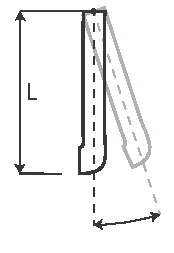
\includegraphics[width=0.18\textwidth]{2015-v2g-05-toru}
 \end{center}
\end{wrapfigure}
Veetoru pikkusega $L$ on kinnitatud seina külge nii, et see saab vertikaaltasandis vabalt pöörelda. Veetoru mass koos seda täitva veega on $M$. Toru ots ristlõikepindalaga $S$ on ülejäänud toruga võrreldes \num{90} kraadi pööratud (vt joonist) ning sellest voolab välja vesi kiirusega $v$ ja tihedusega $\rho$. Kui suure nurga all vertikaali suhtes paikneb toru telg? Raskuskiirenduse väärtus on $g$.
\fi
}

% Ü63
\ylDisplay{Põrge} % Ülesande nimi
{Mihkel Kree} % Autor
{piirkonnavoor} % Voor
{2015} % Aasta
{G 6} % Ülesande nr.
{5} % Raskustase
{
% Teema: Dünaamika
\ifStatement

\begin{wrapfigure}[5]{r}{0.22\textwidth}
 %\vspace{-30pt}
 \begin{center}
 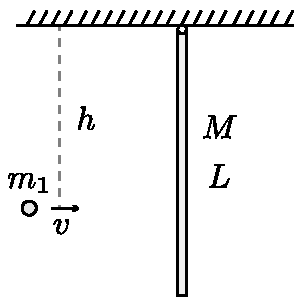
\includegraphics[width=0.22\textwidth]{2015-v2g-06-porgejoonis}
 \end{center}
 %\vspace{-30pt}
\end{wrapfigure}

Algselt paigal olev rippuv varras massiga $M$ ning pikkusega $L$ on fikseeritud ülemisest otsast vabalt pöörleva kinnitusega. Varda inertsimoment otspunkti suhtes on $I=\frac{1}{3}ML^2$. Teraspall massiga $m_1$ lendab vastu varrast ning tabab seda kaugusel $h$ riputuspunktist. Põrge on elastne, st soojuskadudeta. Huvitaval kombel jääb teraskuul pärast põrget hetkeks paigale ning hakkab seejärel vertikaalselt alla langema. Leidke kauguse $h$ väärtus, mille korral niisugune seismajäämine võimalik on.
\fi
}

% Ü64
\ylDisplay{Rattur} % Ülesande nimi
{Ardi Loot} % Autor
{lahtine} % Voor
{2016} % Aasta
{G 6} % Ülesande nr.
{5} % Raskustase
{
% Teema: Dünaamika
\ifStatement
Rattur massiga $m=\SI{100}{kg}$ sõidab ilma väntamata alla mäenõlvalt langemisnurgaga
$\theta_{1}=\SI{4.8}{\degree}$ (nurk horisondi ja mäenõlva vahel)
ja märkab, et piisavalt pika nõlva korral on tema lõppkiiruseks $v_{1}=\SI{50}{km/h}$.
Kaks korda väiksema nõlva korral $(\theta_{2}=\SI{2.4}{\degree})$
on ratturi lõppkiirus aga $\Delta v=\SI{15}{km/h}$ võrra väiksem.
Leidke, kui suur peab olema ratturi väntamise võimsus, et horisontaalsel
teel hoida kiirust $v=\SI{20}{km/h}.$ Kui suur osa võimsusest kulub
tuuletakistuse ületamiseks? Eeldage, et tegemist on tuulevaikse ilmaga
ja raskuskiirendus $g=\SI{9.8}{m/s^{2}}$. 

\emph{Märkus.} Arvestada tuleks nii kiirusest sõltumatu hõõrdejõuga kui ka tuuletakistusega,
mis on võrdeline kiiruse ruuduga.
\fi
}

% Ü65
\ylDisplay{Kaks kuuli ja vedru} % Ülesande nimi
{Rasmus Kisel} % Autor
{piirkonnavoor} % Voor
{2017} % Aasta
{G 7} % Ülesande nr.
{5} % Raskustase
{
% Teema: Dünaamika
\ifStatement
Vedru erinevatesse otstesse on kinnitatud väikesed kuulid, millest ühe mass on $M$ ning teise oma tundmatu. Kogu süsteem pannakse pöörlema nii, et tundmatu massi kaugus pöörlemiskeskmest on võrdne vedru esialgse pikkusega. Mis on selle pöörlemise periood, kui vedru jäikus on $k$? Vedru mass on võrreldes kuulide massidega tühine.
\fi
}

% Ü66
\ylDisplay{Reisirong} % Ülesande nimi
{Moorits Mihkel Muru} % Autor
{lõppvoor} % Voor
{2017} % Aasta
{G 5} % Ülesande nr.
{5} % Raskustase
{
% Teema: Dünaamika
\ifStatement
Reisirong sõidab mööda raudtee ringjoone kaarekujulist lõiku ühtlaselt aeglustudes. Lõigu pikkus on $s$ ja rongil kulub selle läbimiseks aeg $t$. Pärast selle lõigu läbimist on rongi liikumise suund muutunud nurga $\varphi$ võrra ja lõigu alguses oli rongi kiirus $\alpha$ korda suurem, kui see on lõigu lõpus. Leidke seos rongis istuva reisija massi $m$ ja tema kaalu $P$ vahel, kui reisirong on parajasti selle lõigu keskpunktis. Leidke reisija mass, kui $P=\SI{840}{\newton}$, $s=\SI{1.5}{\kilo\meter}$, $t=\SI{60}{\second}$, $\alpha=\num{1.5}$, $\varphi=\SI{60}{\degree}$ ja $g=\SI{9.8}{\meter\per\second\squared}$.
\fi
}

% Ü67
\ylDisplay{Kaheosaline pendel} % Ülesande nimi
{Hans Daniel Kaimre} % Autor
{lõppvoor} % Voor
{2018} % Aasta
{G 4} % Ülesande nr.
{5} % Raskustase
{
% Teema: Dünaamika
\ifStatement
\begin{wrapfigure}[10]{r}{0.4\textwidth}
\vspace{-5pt}
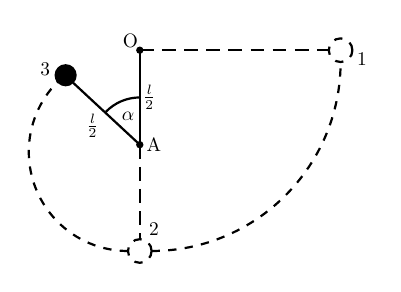
\begin{tikzpicture}[thick,scale=0.6, every node/.style={scale=0.7}]

 % Def. koordinaadid
 \coordinate (O) at (0,0) ;
 \coordinate (1) at (4,0) ;
 \coordinate (A) at (0,-2) ;
 \coordinate (2) at (0,-4);
 \coordinate (3) at (-1.41,-0.69);

 % Jooned, t2pid
 \draw[dash pattern=on5pt off3pt] (O) -- (1);
 \draw[dash pattern=on5pt off3pt] (A) -- (2);
 \draw[thick,dashed] (4.25,0) circle (0.25cm);
 \draw[thick,dashed] (0,-4.25) circle (0.25cm);
 \draw[thick] (O) -- (A);
 \draw[thick] (A) -- (3);
 \filldraw [black] (A) circle (1.5pt);
 \filldraw [black] (O) circle (1.5pt);
 \filldraw [black] (-1.57,-0.53) circle (6pt);
 
 

 % Nurgad ja punktid
 \draw (0,-1) arc (90:136:1);
 \draw[thick, dashed] (0.25,-4.25) arc (270:360:4);
 \draw[thick, dashed] (-0.25,-4.25) arc (270:135:2.1);
 \node[] at (-0.25,-1.4) {$\alpha$};
 \node[] at (4.7,-0.2) {$1$};
 \node[] at (0.3,-3.8) {$2$};
 \node[] at (-2.0,-0.4) {$3$};
 \node[] at (-0.2,0.2) {O};
 \node[] at (0.3,-2) {A};
 \node[] at (0.2,-1) {$\frac{l}{2}$};
 \node[] at (-1,-1.6) {$\frac{l}{2}$};
\end{tikzpicture}
\end{wrapfigure}

Punktis O kinnitatud niidi pikkusega $l$ otsas ripub väike kuulike. Kuulike viiakse kõrvale ja vabastatakse tõuketa asendist 1. Kuuli jõudes asendisse 2, kohtab niit joonise tasandiga risti olevat varrast punktis A, mis asub punktist O kaugusel $l/2$ sellega samal vertikaalil. Leida, millise nurga $\alpha$ väärtuse korral niidi pinge $T=0$ (asend 3). Õhutakistust ja hõõrdumist vardal arvestama ei pea.
\fi
}

% Ü68
\ylDisplay{Veerev pall} % Ülesande nimi
{Hans Daniel Kaimre} % Autor
{piirkonnavoor} % Voor
{2016} % Aasta
{G 8} % Ülesande nr.
{6} % Raskustase
{
% Teema: Dünaamika
\ifStatement
\begin{wrapfigure}{r}{0.3\textwidth}
	\vspace{-15pt}
	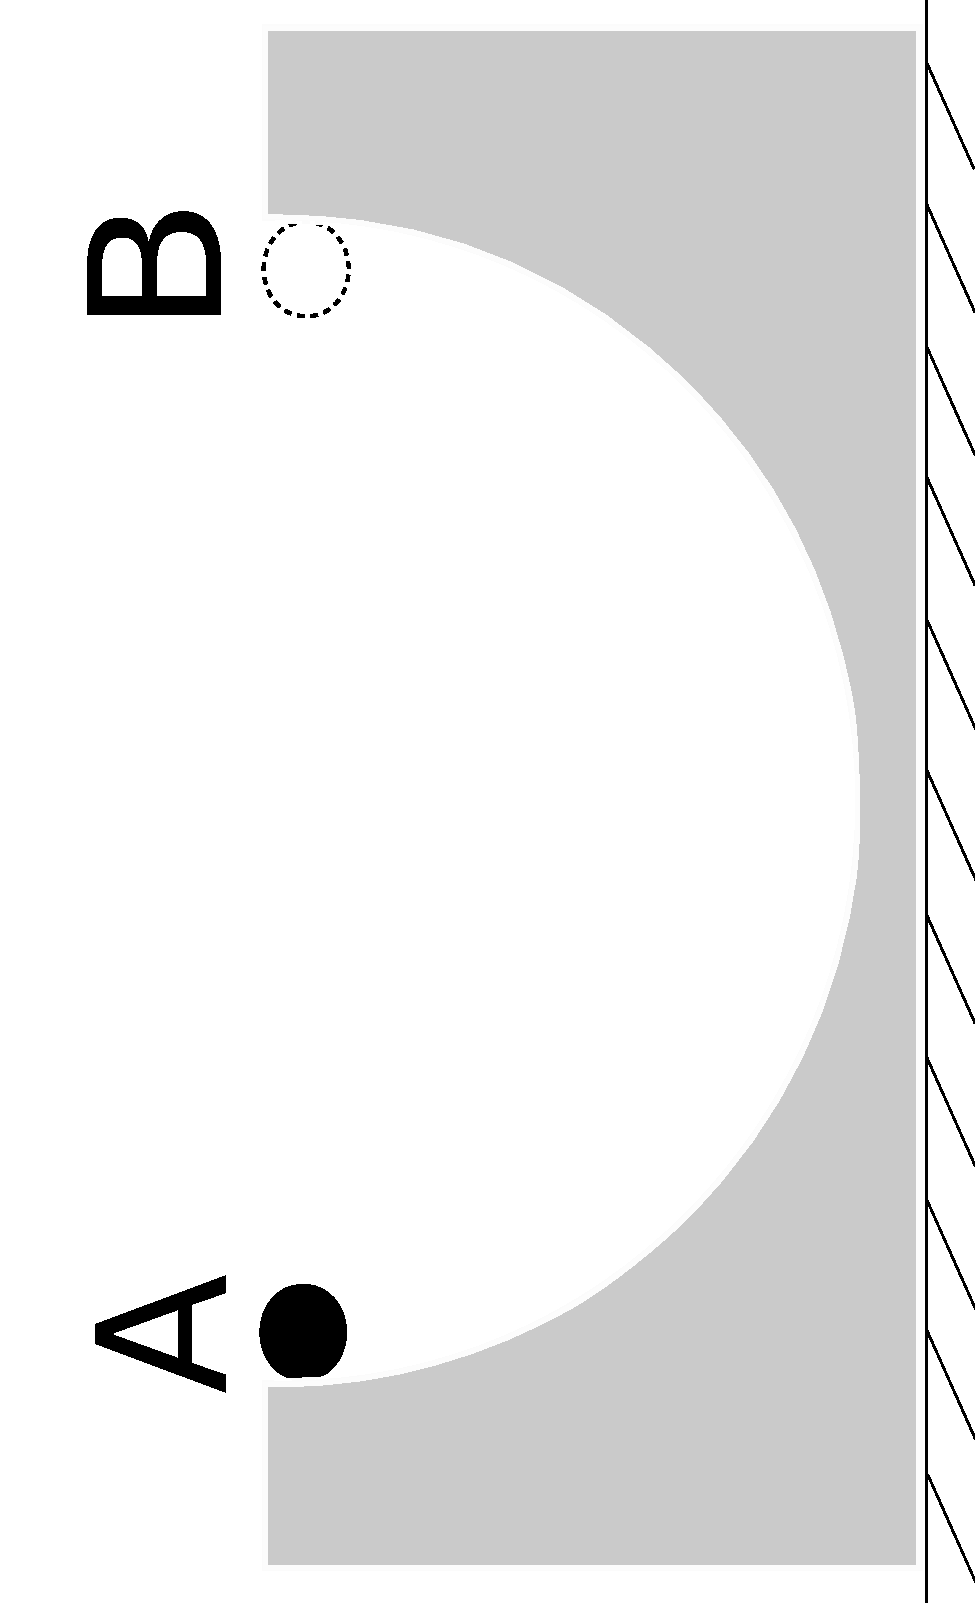
\includegraphics[angle=-90,origin=c,width=0.3\textwidth]{2016-v2g-08-halfpipe.pdf}
\end{wrapfigure}
Klotsist on välja lõigatud poolsilindrikujuline tükk raadiusega $R$. Klots seisab siledal hõõrdevabal horisontaalsel pinnal (vaata joonist). Klotsi mass on $M$. Punktist A lükatakse liikuma mööda silindrikujulise väljalõike pinda väike pall raadiusega $r$ ning massiga $m$. Kui palju on nihkunud klots hetkeks, mil pall jõuab punkti B?
\fi
}

% Ü69
\ylDisplay{Vai} % Ülesande nimi
{Jaak Kikas} % Autor
{piirkonnavoor} % Voor
{2006} % Aasta
{G 10} % Ülesande nr.
{7} % Raskustase
{
% Teema: Dünaamika
\ifStatement
Vertikaalset vaia pikkusega $L$ ja massiga $M$ lüüakse pinnasesse nii, et tema otsa pihta lastakse kõrguselt $H\gg L$ vaia otsast kukkuda koormisel massiga $m$. Lööki vaia pihta võib lugeda absoluutselt mitteelastseks, st pärast raskuse ja vaia kokkupuudet liiguvad nad kui üks tervik. Pinnase takistusjõud on $F = F_0 + kl$, kus $l$ on maa sees oleva vaiaosa pikkus. Kui suur on löökide arv $N$, mis on vajalik selleks, et vai täies pikkuses maasse lüüa? Võite eeldada, et ühekordse löögi tagajärjel nihkub vai sügavamale väikese osa võrra oma pikkusest.
\fi
}

% Ü70
\ylDisplay{Pidurdamine} % Ülesande nimi
{Tanel Kiis} % Autor
{lahtine} % Voor
{2012} % Aasta
{G 7} % Ülesande nr.
{7} % Raskustase
{
% Teema: Dünaamika
\ifStatement
Keha massiga $M$ kukub vabalt raskusjõu toimel kiirendusega~$g$. Tema
kiirust proovitakse muuta, tulistades maalt otse üles iga $t$ sekundi tagant
väikeseid kuulikesi massiga~$m$, mis põrkavad elastselt otse tagasi.
Kui suur peab olema kuulikeste kiirus~$u$, et pärast iga põrget oleks langeva
keha kiirus üks ja seesama~$v$? Võib eeldada, et väikeste kuulikeste kiiruse muut raskusjõu toimel on
tühine ja $m\ll M$.
\fi
}

% Ü71
\ylDisplay{Robin Hood} % Ülesande nimi
{Madis Ollikainen} % Autor
{piirkonnavoor} % Voor
{2012} % Aasta
{G 9} % Ülesande nr.
{7} % Raskustase
{
% Teema: Dünaamika
\ifStatement
Robin Hood on täpsuslaskmisvõistlustel, kus tal tuleb tabada märklauda, mis asub
$L=\SI{200}{m}$ kaugusel. Millise nurga $\alpha$ all horisontaalsihi suhtes
peab Robin vibust laskma, et tabada täpselt märklaua keskpunkti? Vibu vinnamisel
teeb ta tööd $A=\SI{500}{J}$ ning vibu kasutegur on $\eta=0,17$. Noole mass on
$m=\SI{54}{g}$ ja see lastakse lendu märklaua keskpunktist $h=\SI{70}{cm}$ võrra
kõrgemalt. Õhutakistusega ärge arvestage. Raskuskiirenduseks lugege
$g=\SI{9,8}{m/s^2}$.
\fi
}

% Ü72
\ylDisplay{Sportauto} % Ülesande nimi
{Mihkel Rähn} % Autor
{lõppvoor} % Voor
{2014} % Aasta
{G 7} % Ülesande nr.
{7} % Raskustase
{
% Teema: Dünaamika
\ifStatement
Leidke esirattaveolise sõiduauto maksimaalne kiirendus. Auto mass on $m$, esi- ja tagarataste telgede vahe $b$, masskeskme kõrgus $h$ ning masskeskme horisontaalne kaugus tagateljest $s$. Hõõrdetegur rataste ja maa vahel on $\mu$.
\fi
}

% Ü73
\ylDisplay{Latt} % Ülesande nimi
{Kaur Aare Saar} % Autor
{lahtine} % Voor
{2015} % Aasta
{G 8} % Ülesande nr.
{7} % Raskustase
{
% Teema: Dünaamika
\ifStatement
Pikka horisontaaltasapinnal lebavat latti lükatakse ühest otsast muutumatu kiirusega ning risti latiga. Kui kaugel sellest lati otsast asub lati pöörlemistelg? Lati pikkus on $L$. Hõõrdetegur lati ja tasapinna vahel on kõikjal ühesugune.
\fi
}

% Ü74
\ylDisplay{Klaaskuul} % Ülesande nimi
{Aigar Vaigu} % Autor
{piirkonnavoor} % Voor
{2008} % Aasta
{G 6} % Ülesande nr.
{8} % Raskustase
{
% Teema: Dünaamika
\ifStatement
Klaaskuul kukkus vertikaalselt alla libedale horisontaalsele põrandale ning purunes kolmeks tükiks, mis lendasid mööda põrandat laiali. Sündmus jäädvustati fotol (vt joonist). Tükkide kujutised osutusid välja venitatuks, sest säriaeg oli võrdlemisi pikk. Millised olid kuuli tükkide masside suhted? Hõõrdejõud tükkide liikumisel lugeda tühiselt väikeseks. Fotoobjektiivi optiline peatelg oli pildistamisel vertikaalne

\begin{center}
	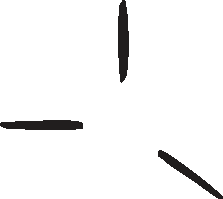
\includegraphics[width=0.6\linewidth]{2008-v2g-06-yl}
\end{center}
\fi
}

% Ü75
\ylDisplay{Plokid} % Ülesande nimi
{Mihkel Kree} % Autor
{piirkonnavoor} % Voor
{2008} % Aasta
{G 9} % Ülesande nr.
{8} % Raskustase
{
% Teema: Dünaamika
\ifStatement
Polüspast ehk liitplokk koosneb seitsmest plokist (vt. joonist). Koormiste massid $M$ ja $\gamma M$ on näidatud joonisel. Missuguse kiirendusega hakkavad liikuma äärmised koormised? Mis tingimust peab rahuldama suurus $\gamma$, et äärmised koormised hakkaksid langema? Plokkide ja nööri mass jätta arvestamata ning nöör lugeda venimatuks. 

\begin{center}
	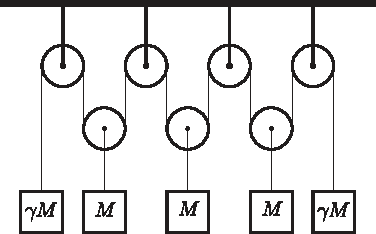
\includegraphics[width=0.6\linewidth]{2008-v2g-09-yl}
\end{center}
\fi
}

% Ü76
\ylDisplay{Õõnes kera} % Ülesande nimi
{Tanel Kiis} % Autor
{piirkonnavoor} % Voor
{2013} % Aasta
{G 9} % Ülesande nr.
{8} % Raskustase
{
% Teema: Dünaamika
\ifStatement
Jukul on rauast kera
($\varrho_\mathrm{Fe}=\SI{7,9}{\gram\per\centi\meter\cubed}$) raadiusega
$r=\SI{10}{\centi\meter}$ ja massiga $m=\SI{30}{\kilo\gram}$. Juku teab, et kera
sees on sfääriline õõnsus, mille keskpunkti kaugust $d$ kera keskpunktist ta üritab
leida. Selleks riputas ta kuuli kaks korda nööri otsa rippuma, kasutades
riputuskohtadeks kera vastaspunkte. Ühel korral moodustas neid kinnituspunkte
ühendav telg horisondiga nurga $\alpha=\SI{60}{\degree}$, teisel korral aga nurga
$\beta=\SI{45}{\degree}$. Leidke $d$.
\fi
}

% Ü77
\ylDisplay{Jalgpallurid} % Ülesande nimi
{Andreas Valdmann} % Autor
{lõppvoor} % Voor
{2013} % Aasta
{G 9} % Ülesande nr.
{8} % Raskustase
{
% Teema: Dünaamika
\ifStatement
Kaks jalgpallurit proovisid trikilööki, kus kaks palli õhus kokku põrkavad.
Jalgpallurid seisid teineteisest $d = \SI{20}{m}$ kaugusel ja andsid samal ajahetkel
sooritatud löögiga kumbki oma pallile algkiiruse $v = \SI{15}{m/s}$. Mis piirkonnas võisid pallid lennul kokku põrgata?
Vastuseks tehke pealtvaates joonis, kuhu on kantud jalgpallurite
asukohad ja kõikvõimalike kokkupõrkepunktide piirkond. Esitage ka selle
piirkonna mõõdud. Võimalike kokkupõrkepunktide kõrgust maapinnast pole
vaja eraldi välja arvutada ega joonisele kanda. Raskuskiirendus
on $g = \SI{9,8}{m/s^2}$. 
\fi
}

% Ü78
\ylDisplay{Mutrivõti} % Ülesande nimi
{Andres Põldaru} % Autor
{lahtine} % Voor
{2015} % Aasta
{G 9} % Ülesande nr.
{8} % Raskustase
{
% Teema: Dünaamika
\ifStatement
Kui suur peab olema reguleeritava mutrivõtme keerete arv pikkusühiku kohta $n$, et mutreid saaks kõvasti kinni keerata? Hõõrdetegur kokkupuutepindade vahel on $\mu$ ja raadius reguleerija teljest kokkupuutepinnani on $r$.
\begin{center}%
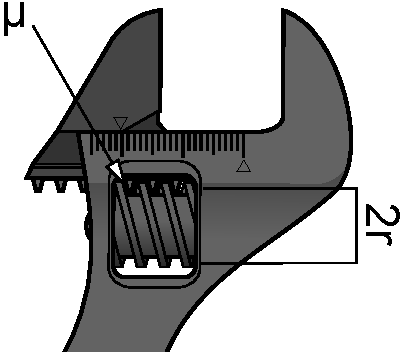
\includegraphics[width=0.4\linewidth]{2015-lahg-09-mutriv6ti_joonis}%
\end{center}
\fi
}

% Ü79
\ylDisplay{Plokid} % Ülesande nimi
{Taavet Kalda} % Autor
{lahtine} % Voor
{2017} % Aasta
{G 8} % Ülesande nr.
{8} % Raskustase
{
% Teema: Dünaamika
\ifStatement
Joonisel on kujutatud kahest plokist ja kolmest raskusest, massidega $m_1$, $m_2$ ja $M$ koosnevat süsteemi. Nöörid on venimatud ning nööride ja plokkide massid on tühised võrreldes raskuste massidega. Hõõre ploki ja nööri vahel on tühiselt väike. Missugune peaks olema $M$ väärtus selleks, et $M$ jääks esialgu paigale, kui süsteem lahti lasta?

\begin{center}
	\vspace{-10pt}
	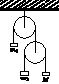
\includegraphics[width = 0.3\linewidth] {2017-lahg-08-double_pulleys_img.pdf}
\end{center}
\fi
}

% Ü80
\ylDisplay{Mänguauto} % Ülesande nimi
{Jaan Kalda} % Autor
{lahtine} % Voor
{2017} % Aasta
{G 9} % Ülesande nr.
{8} % Raskustase
{
% Teema: Dünaamika
\ifStatement
Mänguauto telgede vaheline kaugus on $L$ ning massikese asub võrdsel kaugusel telgedest kõrgusel $h$ horisontaalpinnast. Auto esimesed rattad saavad vabalt pöörelda ja on tühise massiga, tagumised rattad on aga jäigalt kinni kiilunud ega pöörle üldse. Auto lebab horisontaalsel pinnal, rataste ja horisontaalpinna vaheline hõõrdetegur on $\mu$, raskuskiirendus on $g$.

Horisontaalpinda hakatakse liigutama kõrge sagedusega horisontaalselt edasi-tagasi: ühe poolperioodi jooksul on pinna kiirusvektor suunatud auto tagaratastelt esiratastele ning teise poolperioodi jooksul on see vastassuunaline; mõlema poolperioodi jooksul püsib kiiruse moodul konstantsena; võngutamisel liigutatakse pinda nii kiiresti, et auto libiseb pinna suhtes kogu aeg kas ühes või teises suunas. Millise keskmise kiirendusega hakkab liikuma auto?
\fi
}

% Ü81
\ylDisplay{Rong} % Ülesande nimi
{Tundmatu autor} % Autor
{lahtine} % Voor
{2006} % Aasta
{G 10} % Ülesande nr.
{9} % Raskustase
{
% Teema: Dünaamika
\ifStatement
Rong sõidab kiirusega $v = \SI{100}{km/h}$ ja pidurdab järsult (blokeerides rattad). Graafikul on toodud rongi rataste ja rööbaste vahelise hõõrdeteguri $\mu$ sõltuvus kiirusest (\si{km/h}).\\
\osa Kui pikk on rongi täieliku peatumiseni kulunud aeg?\\
\osa Kui suur on pidurdusmaa pikkus? Mõlemad vastused tuleb leida
graafikualuste pindaladena sobilikult valitud teljestikes.

\begin{center}
	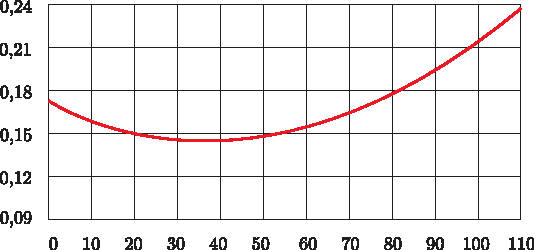
\includegraphics[width=\linewidth]{2006-lahg-10-yl}
\end{center}
\fi
}

% Ü82
\ylDisplay{Värinaalarm} % Ülesande nimi
{Jaan Kalda} % Autor
{lahtine} % Voor
{2011} % Aasta
{G 9} % Ülesande nr.
{9} % Raskustase
{
% Teema: Dünaamika
\ifStatement
Uurime mobiiltelefoni liikumist nõrgalt kaldus pinnal värinaalarmi töötamise
ajal lihtsustatud mudeli abil.
Kujutagu lauale asetatud mobiil risttahukat massiga $M$, mille sees liigub
üles-alla väike keha massiga $m$.
Liikugu see keha ajahetkedel $t=0, 2\tau, 4\tau, \ldots$ vahemaa $x$ võrra
hetkeliselt üles ning ajahetkedel $t=\tau, 3\tau, 5\tau, \ldots$ algasendisse
tagasi.
Olgu mobiiltelefoni ja laua vaheline hõõrdetegur $\mu$ ning laua kaldenurk
$\alpha \ll 1$. Mobiiltelefoni ja laua vahelised põrked lugege absoluutselt
plastseiks.
Millise keskmise kiirusega $u$ hakkab mobiiltelefon mööda lauda liikuma?
\fi
}

% Ü83
\ylDisplay{Killud} % Ülesande nimi
{Jaan Kalda} % Autor
{lahtine} % Voor
{2012} % Aasta
{G 10} % Ülesanne nr.
{9} % Raskustase
{
% Teema: Dünaamika
\ifStatement
Savikuulike massiga \SI{10}{g} kukkus vertikaalselt alla siledale horisontaalsele
põrandale ja läks kolmeks killuks.
Killud lendasid laiali ja peatusid punktides, mis on näidatud juuresoleval
joonisel
(ülaltvaade, ristiga on märgitud kukkumiskoht). Määrake kildude massid.
Joonisel (lisalehel)
võib teha lisakonstruktsioone ja mõõtmisi.
Võite lugeda, et killud hakkasid kohe pärast kukkumist üles põrkumata libisema,
õhuhõõre on tühine ja liugehõõrdetegur ei sõltu kiirusest.
\begin{center}
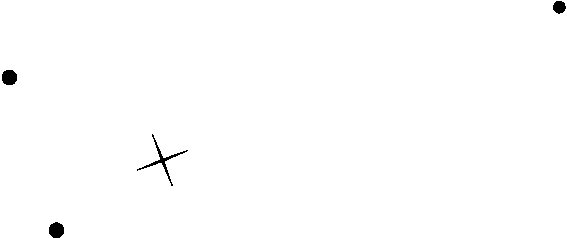
\includegraphics[width=0.8\linewidth]{2012-lahg-10-killud}
\end{center}
\fi
}

% Ü84
\ylDisplay{Liivakell} % Ülesande nimi
{Roland Matt} % Autor
{lõppvoor} % Voor
{2012} % Aasta
{G 8} % Ülesande nr.
{9} % Raskustase
{
% Teema: Dünaamika
\ifStatement
Uurime liivakella mudelit. Liivakell koosneb silindrilisest torust pikkusega
$L$, mis on keskelt eraldatud ühtlaselt aukudega läbistatud plaadiga, millest
liiv saab läbi voolata. Heas lähenduses ei sõltu liiva aukude läbimise
masskiirus $w$ ülemises anumas olevast liivahulgast. Liivakell asetatakse
kaalule töörežiimis (kui liiv voolab) ja siis, kui kogu liiv on alla voolanud.
Milline on kaalunäitude vahe? Liiva tihedus on $\rho$ ja liivakella
ristlõikepindala on $S$. Eeldage, et hetkel kukkuva liiva mass on tühine
võrreldes liiva kogumassiga.
\fi
}

% Ü85
\ylDisplay{Silindrilised anumad} % Ülesande nimi
{Jaan Kalda} % Autor
{lõppvoor} % Voor
{2014} % Aasta
{G 8} % Ülesande nr.
{9} % Raskustase
{
% Teema: Dünaamika
\ifStatement
\begin{wrapfigure}{r}{0.07\textwidth}%
\vspace{-15pt}
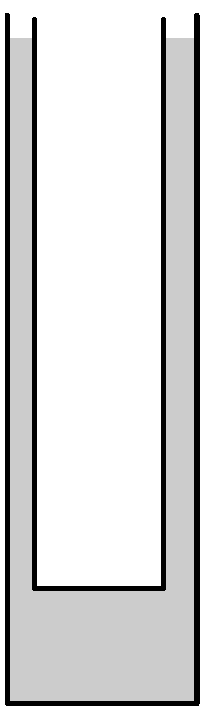
\includegraphics[width=1\linewidth]{2014-v3g-08-cylinders}
\end{wrapfigure}

Silindriline anum siseraadiusega $R = \SI{30}{mm}$ on täidetud veega. Teine tühi silindriline anum raadiusega $r =\SI{25}{mm}$, mille mass on tühiselt väike, on surutud koaksiaalselt suurema silindri sisse nii, et selle vettesukeldunud osa pikkus $L = \SI{300}{mm}$ (vt joonist). Leidke sisemise silindri kiirendus vahetult pärast seda, kui see vabaks lastakse. Vee pindpinevuse ning viskoossusega arvestada pole tarvis.
\fi
}

% Ü86
\ylDisplay{Vedru} % Ülesande nimi
{Mihkel Kree} % Autor
{lõppvoor} % Voor
{2015} % Aasta
{G 8} % Ülesande nr.
{9} % Raskustase
{
% Teema: Dünaamika
\ifStatement
Kasti sees on vedru külge riputatud koormis. Nii kast kui koormis on massiga $m$. Vedru mass on tühiselt väike ning selle jäikustegur on $k$. Kastil lastakse kõrguselt $h$ vabalt maha kukkuda nii, et langemise ajal on koormis tasakaaluolekus. Kokkupõrkel pehme pinnaga jääb kast hetkeliselt paigale. Kast on piisavalt kõrge selleks, et koormis vastu kasti ei põrkaks. Vedrut ei suruta ühelgi hetkel täielikult kokku.\\
\osa Milline on vähim kõrgus $h_\text{m}$, millelt kukkudes hüppab kast tagasi üles?\\
\osa Kastil lasti kukkuda punktis a) leitud algkõrguselt $h\approx h_\text{m}$. Kui pika ajavahemiku $t$ veedab kast maapinnal enne üles kerkimist? 

\emph{Märkus.} Pange tähele, et vabalangemises olev koormis on kaaluta olekus ning seetõttu on vedru langemise ajal välja venitamata. Maapinnale jõudes pole koormis enam tasakaaluasendis ning hakkab seetõttu uue tasakaaluasendi ümber võnkuma nurksagedusega $\omega =\sqrt{\frac{k}{m}}$.
\fi
}

% Ü87
\ylDisplay{Vardad} % Ülesande nimi
{Jaan Kalda} % Autor
{lahtine} % Voor
{2017} % Aasta
{G 10} % Ülesande nr.
{9} % Raskustase
{
% Teema: Dünaamika
\ifStatement
\begin{wrapfigure}[7]{r}{0.4\textwidth}
	\vspace{-10pt}
	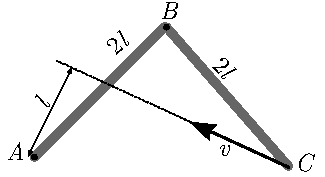
\includegraphics[width = 0.4\textwidth] {2017-lahg-10-delta.pdf}
\end{wrapfigure}

Juuresoleval joonisel on kujutatud kahest vardast pikkusega $2l$ koostatud \v sarniirne konstruktsioon. Ühe varda otspunkt on fikseeritud liikumatuna punkti $A$ ning teise varda otspunkt $C$ liigub konstantse kiirusega $v$ piki sihti, mis möödub punktist $A$ kaugusel $l$. Leidke varraste ühenduspunkti $B$ kiirendus hetkel, mil punktide $A$ ja $C$ vahekaugus on $2l$.
\fi
}

% Ü88
\ylDisplay{Kuulid} % Ülesande nimi
{Jaan Kalda} % Autor
{lõppvoor} % Voor
{2006} % Aasta
{G 10} % Ülesande nr.
{10} % Raskustase
{
% Teema: Dünaamika
\ifStatement
\begin{wrapfigure}[8]{r}{0.3\textwidth}
	\begin{center}
		\vspace{-25pt}
		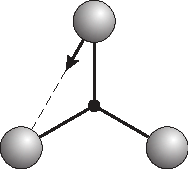
\includegraphics[width=\linewidth]{2006-v3g-10-yl}
	\end{center}
\end{wrapfigure}
Joonisel kujutatud süsteem koosneb kolmest võrdkülgse kolmnurga tippudes paiknevast kuulist massiga $m$ ja kolmest kergest vardast pikkusega $l$, mis on omavahel šarniirselt ühendatud (liigendiga). Süsteem lebab hõõrdevabalt siledal horisontaalpinnal. Ühte kuuli lükatakse teatud lühiajalise jõuga nii, et see omandab kiiruse $v_0$, mis on suunatud naaberkuuli poole. Leidke teiste kuulide kiiruste suunad ja moodulid ning kõigi kuulide kiirendused vahetult peale esimese kuuli lükkamist.
\fi
}
\newpage\subsection{\protect\StrSubstitute{Elektriahelad}{-}{ }}

% Ü89
\ylDisplay{Mõõteriistad} % Ülesande nimi
{Koit Timpmann} % Autor
{lõppvoor} % Voor
{2006} % Aasta
{G 1} % Ülesande nr.
{1} % Raskustase
{
% Teema: Elektriahelad
\ifStatement
Vooluringis on ampermeeter ja voltmeeter ühendatud jadamisi. Klemmidele on rakendatud pinge $U = \SI{9}{V}$. Kui voltmeetriga ühendada rööbiti takisti $R$, väheneb voltmeetri näit kaks korda, ampermeetri näit aga suureneb kaks korda. Kui suurt pinget näitas voltmeeter enne ja pärast takisti ühendamist?

\begin{center}
	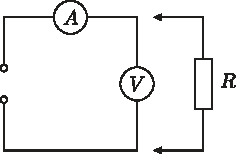
\includegraphics[width=0.5\linewidth]{2006-v3g-01-yl}
\end{center}
\fi
}

% Ü90
\ylDisplay{Voltmeetrid} % Ülesande nimi
{Eero Vaher} % Autor
{piirkonnavoor} % Voor
{2016} % Aasta
{G 1} % Ülesande nr.
{1} % Raskustase
{
% Teema: Elektriahelad
\ifStatement
Elektriskeemis on pingeallikas pingega $U_0=\SI{30}{V}$ ning neli ühesugust voltmeetrit. Kui suur on iga voltmeetri näit?

\begin{center}
	\tikzset{component/.style={draw,thick,circle,fill=white,minimum size =0.75cm,inner sep=0pt}}
	\begin{resizebox}{0.45\linewidth}{!}{
		\begin{circuitikz}
			\draw
			
			(6,0) to[battery1,l=${U_0=\SI{30}{V}}$] (0,0) to (0,2) to (6,2) to (6,0)
			(2,2) to[short, *-] (2,3) to (6,3) to[short, -*] (6,2)
			;
			\node[component] at (1,2) {V$_1$};
			\node[component] at (3,2) {V$_2$};
			\node[component] at (5,2) {V$_3$};
			\node[component] at (4,3) {V$_4$};
		\end{circuitikz}}
	\end{resizebox}
\end{center}
\fi
}

% Ü91
\ylDisplay{Voltmeeter} % Ülesande nimi
{Erkki Tempel} % Autor
{piirkonnavoor} % Voor
{2017} % Aasta
{G 1} % Ülesande nr.
{1} % Raskustase
{
% Teema: Elektriahelad
\ifStatement
Joonisel näidatud elektriskeemis on ideaalne ampermeeter, mis näitab voolutugevust $I$. Ampermeeter asendatakse ideaalse voltmeetriga. Kui suur on voltmeetri näit? Kõikide takistite takistus on $R$.
\begin{center}
	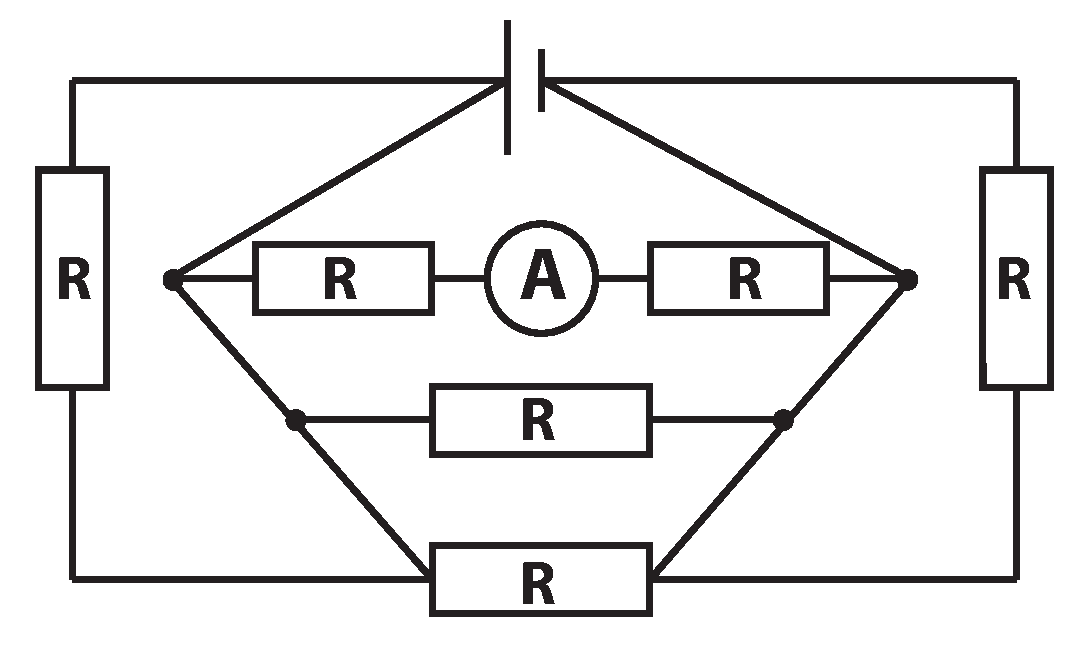
\includegraphics[width=0.4\textwidth]{2017-v2g-01-skeem}
\end{center}
\fi
}

% Ü92
\ylDisplay{Elektriküünlad} % Ülesande nimi
{Valter Kiisk} % Autor
{piirkonnavoor} % Voor
{2009} % Aasta
{G 4} % Ülesande nr.
{2} % Raskustase
{
% Teema: Elektriahelad
\ifStatement
Jõulukaunistuse valmistamiseks otsis Juku välja 10
taskulambipirni (nimipinge \SI{3}V, võimsus \SI{0.6}W) ja alaldi klemmipingega \SI{5}V.
Seejärel koostas ta skeemi, mis on kujutatud joonisel.\\
\osa Kui suur peab olema
takisti $R$ takistus, et pinge lampidel ei ületaks nimipinget?\\
\osa Skeemi sisselülitamisel avastas Juku, et lambid põlevad oodatust tuhmimalt. Selgus, et alaldi
klemmipinge oli koormusega langenud \SI{4}V-ni ning pinge lampidel \SI{2,3}V-ni. Kui suur
tuleks valida takisti $R$ väärtus, et lambid põleksid normaalse heledusega?

\begin{center}
	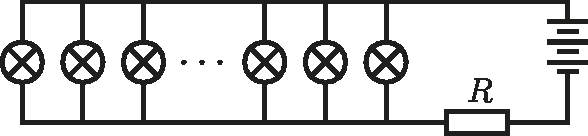
\includegraphics[width=0.8\linewidth]{2009-v2g-04-yl}
\end{center}
\fi
}

% Ü93
\ylDisplay{Päikesepaneel} % Ülesande nimi
{Mihkel Pajusalu} % Autor
{lõppvoor} % Voor
{2010} % Aasta
{G 3} % Ülesande nr.
{2} % Raskustase
{
% Teema: Elektriahelad
\ifStatement
Joonisel on kujutatud päikesepaneeli läbiva voolu sõltuvus klemmipingest.
Määrake paneeli klemmidega ühendatud koormise takistus, mille korral on koormisel eralduv
võimsus maksimaalne.

\begin{center}
	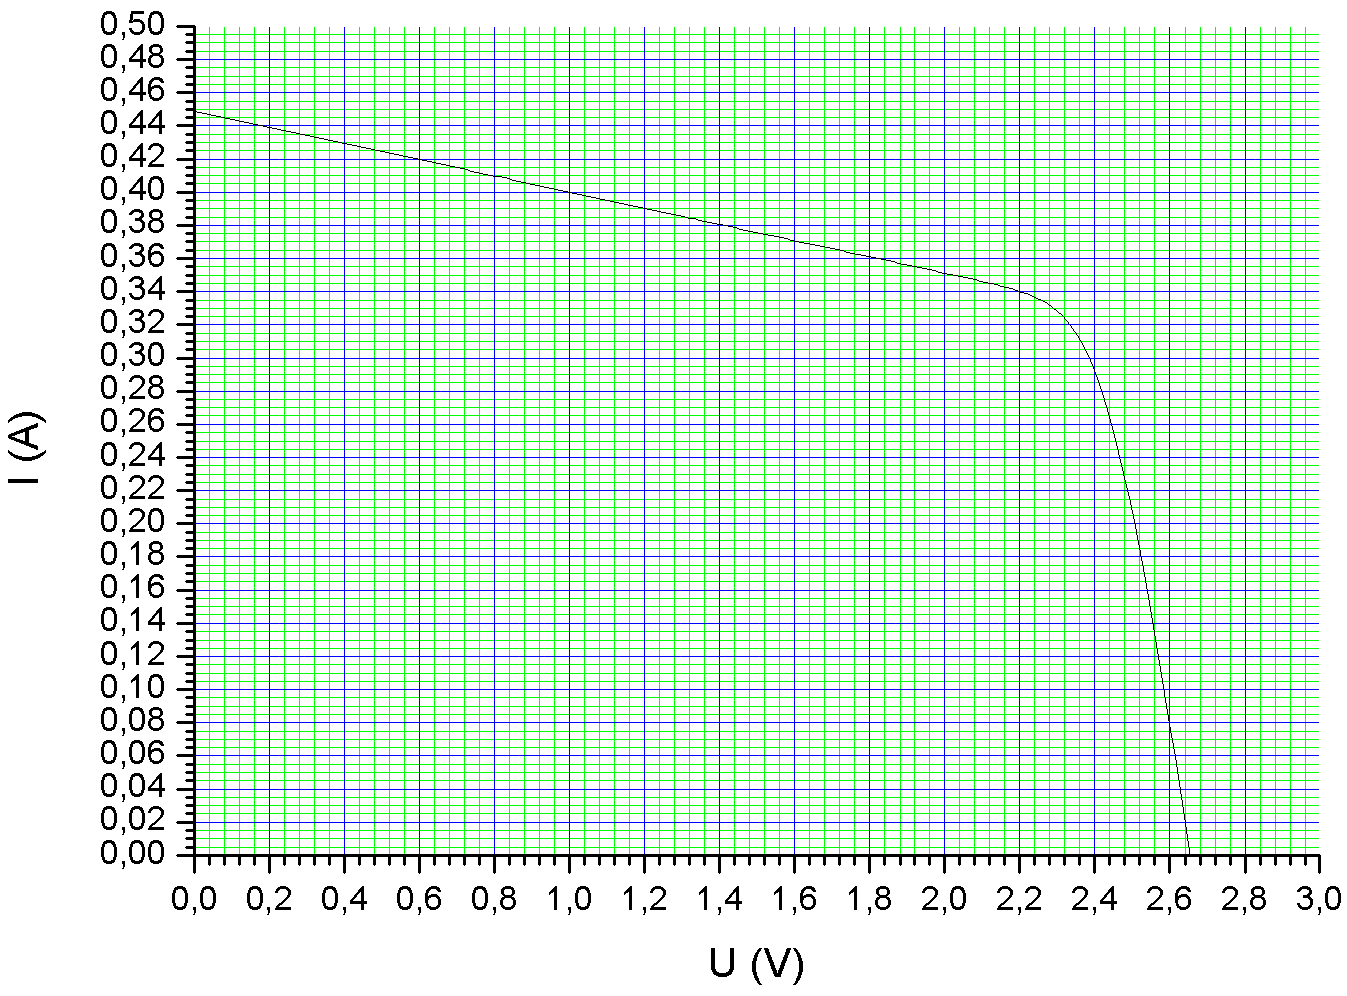
\includegraphics[width=0.9\linewidth]{2010-v3g-03-paneel_yl.png}
\end{center}
\fi
}

% Ü94
\ylDisplay{Lambid} % Ülesande nimi
{Mihkel Kree} % Autor
{piirkonnavoor} % Voor
{2015} % Aasta
{G 2} % Ülesande nr.
{2} % Raskustase
{
% Teema: Elektriahelad
\ifStatement
Pingeallikaga on rööbiti ühendatud kaks lampi, kusjuures üks lampidest põleb $k$ korda suurema võimsusega kui teine. Seejärel ühendatakse need lambid sama pingeallikaga jadamisi. Mitu korda muutub lampidel eralduv koguvõimsus? Kas see muutub suuremaks või väiksemaks?
\pagebreak
\fi
}

% Ü95
\ylDisplay{Ampermeetrid} % Ülesande nimi
{Tundmatu autor} % Autor
{lahtine} % Voor
{2008} % Aasta
{G 4} % Ülesande nr.
{3} % Raskustase
{
% Teema: Elektriahelad
\ifStatement
Vooluahelasse on ühendatud neli ühesugust ampermeetrit, igaüks sisetakistusega $r$, ja takisti $R$. Esimese kahe ampermeetri näidud on $I_1= \SI{3}{A}$ ja $I_2= \SI{5}{A}$. Leida takistuste suhte $R/r$ arvuline väärtus.

\begin{center}
	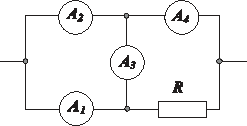
\includegraphics[width=0.6\linewidth]{2008-lahg-04-yl}
\end{center}
\fi
}

% Ü96
\ylDisplay{Patarei} % Ülesande nimi
{Taavi Pungas} % Autor
{piirkonnavoor} % Voor
{2011} % Aasta
{G 6} % Ülesande nr.
{3} % Raskustase
{
% Teema: Elektriahelad
\ifStatement
Patarei ühendatakse jadamisi takistiga takistusega $R$ ja ampermeetriga, mis näitab voolutugevuseks $I_1$. Kui lisada jadamisi veel üks takisti takistusega $R$, näitab ampermeeter voolutugevuseks $I_2$. Leidke, mis vahemikku jääks suhe $I_2/I_1$, kui vooluallika sisetakistus $r$ oleks\\
\osa väiksem kui $R$,\\
\osa suurem kui $R$.
\fi
}

% Ü97
\ylDisplay{Elektriskeem} % Ülesande nimi
{Oleg Košik} % Autor
{piirkonnavoor} % Voor
{2013} % Aasta
{G 5} % Ülesande nr.
{3} % Raskustase
{
% Teema: Elektriahelad
\ifStatement
\begin{wrapfigure}[7]{r}{2.5cm}%
\vspace{-12pt}
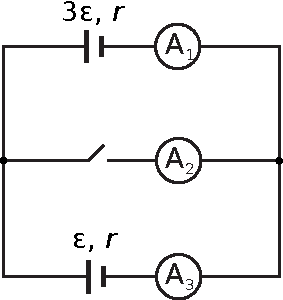
\includegraphics[width=\linewidth]{2013-v2g-05-skeem}%
\end{wrapfigure}
Joonisel toodud skeemil on ampermeetrid ideaalsed; patareide elektromotoorjõud
ja sisetakistused on märgitud nende juurde. Leidke ampermeetrite näidud, kui\\
\osa lüliti on suletud;\\
\osa lüliti on lahti.\\
\emph{Märkus}. praktikas tohib
sellist skeemi kasutada vaid siis, kui ollakse veendunud, et tekkivad voolud
jäävad ampermeetrite mõõtepiirkonda!
\fi
}

% Ü98
\ylDisplay{Tetraeeder} % Ülesande nimi
{Eero Vaher} % Autor
{lahtine} % Voor
{2014} % Aasta
{G 4} % Ülesande nr.
{3} % Raskustase
{
% Teema: Elektriahelad
\ifStatement
Tetraeedri (neljast võrdkülgsest kolmnurgast koosneva püramiidi) servadeks on ühesugused takistid takistusega $R$. Leidke tetraeedri kahe tipu vaheline takistus.
\fi
}

% Ü99
\ylDisplay{Ruudustik} % Ülesande nimi
{Taavi Pungas} % Autor
{lõppvoor} % Voor
{2014} % Aasta
{G 1} % Ülesande nr.
{3} % Raskustase
{
% Teema: Elektriahelad
\ifStatement
Traadist on valmistatud 2x2 ruudustik (vt joonist), iga väikese ruudu külje takistus on $r=\SI{1}{\ohm}$. Leidke punktide A ja B vaheline takistus.

\begin{center}
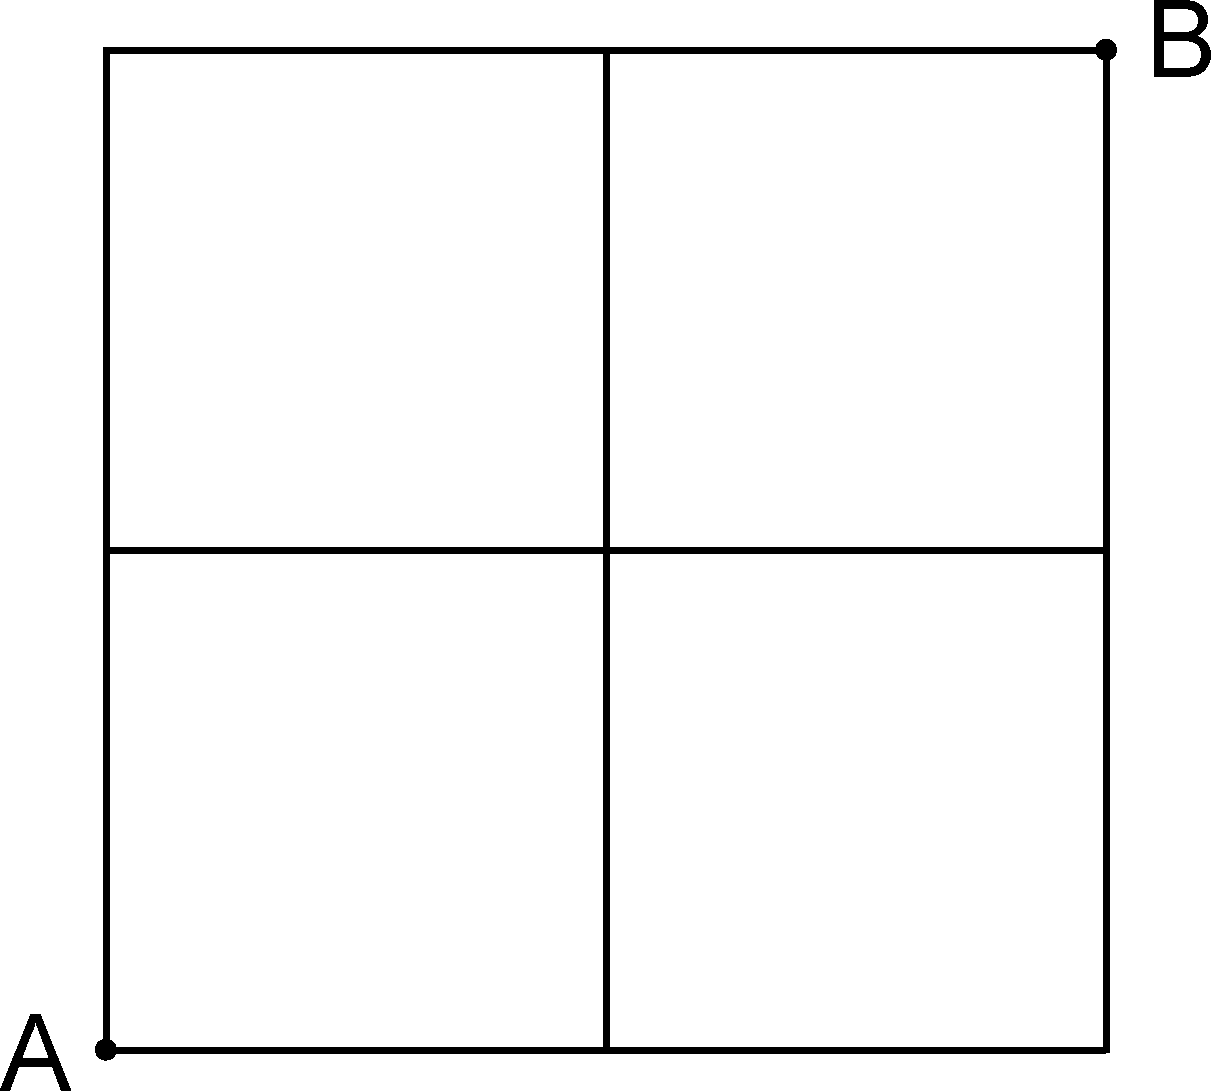
\includegraphics[width=0.2\linewidth]{2014-v3g-01-ruudustik}
\end{center}
\fi
}

% Ü100
\ylDisplay{Takistid} % Ülesande nimi
{Hans Daniel Kaimre} % Autor
{lahtine} % Voor
{2015} % Aasta
{G 2} % Ülesande nr.
{3} % Raskustase
{
% Teema: Elektriahelad
\ifStatement
Leidke ühesugustest takistitest koosneva ahela kogutakistus $R_{AB}$. Iga takisti takistus on $R$.

\begin{figure}[h]
\centering
\begin{circuitikz}[scale=0.9] \draw

(0,0) to [resistor] (0,2)
(0,0) to [resistor] (0,-2)
(0,0) to [resistor, *-*] (2,0)
(2,0) to [resistor] (4,0)
(4,0) to [resistor, *-*] (6,0)
(2,0) to [resistor, -*] (2,2)
(2,0) to [resistor, -*] (2,-2)
(4,0) to [resistor, -*] (4,2)
(4,0) to [resistor, -*] (4,-2)
(-1,0) to [short,o-] (0,0)
(6,0) to [short,-o] (7,0)
(0,2) -- (6,2) -- (6,0) -- (6,-2) -- (0,-2)
(-1,0) node[label={above:A}] {}
(7,0) node[label={above:B}] {}
;
\end{circuitikz}
\end{figure}
\fi
}

% Ü101
\ylDisplay{Elektriskeem} % Ülesande nimi
{Kristian Kuppart} % Autor
{lahtine} % Voor
{2016} % Aasta
{G 3} % Ülesande nr.
{3} % Raskustase
{
% Teema: Elektriahelad
\ifStatement

Leidke juuresoleval skeemil voolutugevus $I$ läbi ampermeetri kahel juhul: vahetult pärast lüliti sulgemist ja pika aja möödumisel. Eeldada, et kondensaatorid on enne lüliti sulgemist laadimata. Patarei lugeda ideaalseks.
\begin{center}
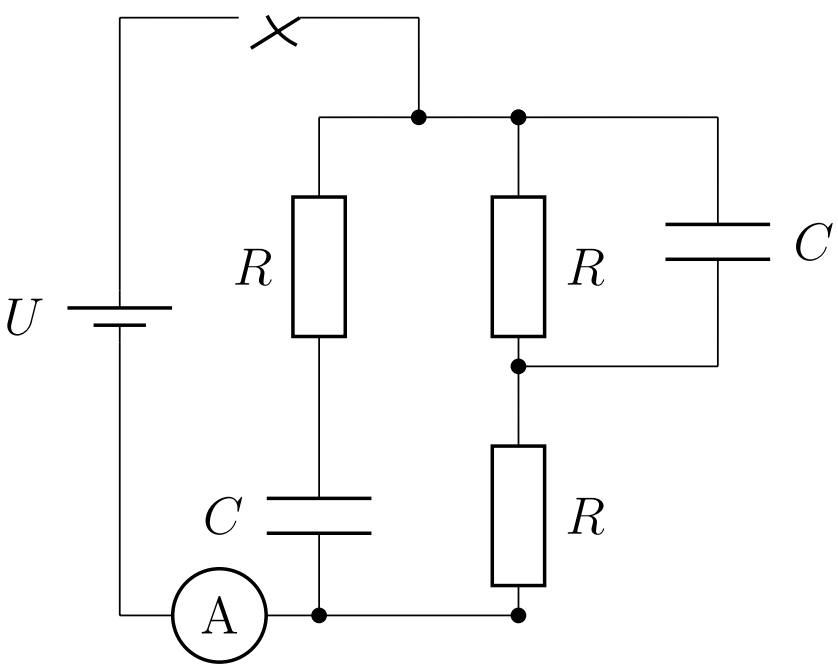
\includegraphics[width=0.45\textwidth]{2016-lahg-03-skeemjoonis.png}
\end{center}
\fi
}

% Ü102
\ylDisplay{Vooluring} % Ülesande nimi
{Valter Kiisk} % Autor
{piirkonnavoor} % Voor
{2005} % Aasta
{G 4} % Ülesande nr.
{4} % Raskustase
{
% Teema: Elektriahelad
\ifStatement
Takisti takistuse määramiseks koostati kaks erinevat vooluringi kasutades voltmeetrit, ampermeetrit ja vooluallikat (vt joonist). Leidke avaldis takistuse $R$ arvutamiseks, kui vasakpoolse skeemi järgi mõõtes saadi voltmeetri näiduks $U_1$ ja ampermeetri näiduks $I_1$ ning parempoolse skeemi järgi mõõtes aga vastavalt $U_2$ ja $I_2$. Vooluallika elektromotoorjõud on muutumatu ning sisetakistus tühine. Mõõteriistade sisetakistused ei ole teada.

\begin{figure}[h]
	\centering
	\begin{minipage}[b]{0.25\textwidth}
		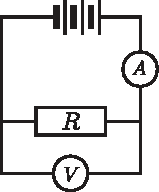
\includegraphics[width=\linewidth]{2005-v2g-04-yl1}
	\end{minipage}
	\hspace{30pt}
	\begin{minipage}[b]{0.3\textwidth}
		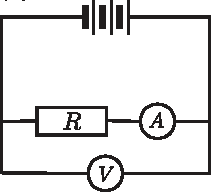
\includegraphics[width=\linewidth]{2005-v2g-04-yl2}
    \end{minipage}
\end{figure}

\fi
}

% Ü103
\ylDisplay{Takistid} % Ülesande nimi
{Aigar Vaigu} % Autor
{lõppvoor} % Voor
{2005} % Aasta
{G 4} % Ülesande nr.
{4} % Raskustase
{
% Teema: Elektriahelad
\ifStatement
Mitu korda muutub joonisel kujutatud ahelas takistil $A$ eralduv võimsus, kui vahetada alalispingeallika polaarsus? Kõik takistid on võrdse takistusega.

\begin{center}
	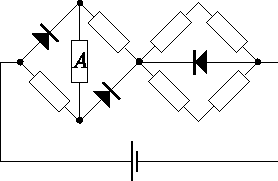
\includegraphics[width=0.6\linewidth]{2005-v3g-04-yl}
\end{center}
\fi
}

% Ü104
\ylDisplay{Elektriskeem} % Ülesande nimi
{Tundmatu autor} % Autor
{lahtine} % Voor
{2006} % Aasta
{G 2} % Ülesande nr.
{4} % Raskustase
{
% Teema: Elektriahelad
\ifStatement
Leida laengud $q_1$, $q_2$ ja $q_3$ kõikidel skeemil toodud kondensaatoritel.

\begin{center}
	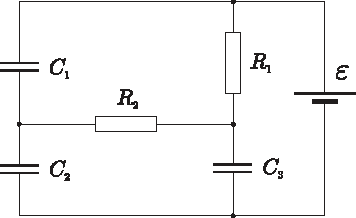
\includegraphics[width=0.7\linewidth]{2006-lahg-02-yl}
\end{center}
\fi
}

% Ü105
\ylDisplay{Skeem} % Ülesande nimi
{Tundmatu autor} % Autor
{lahtine} % Voor
{2009} % Aasta
{G 3} % Ülesande nr.
{4} % Raskustase
{
% Teema: Elektriahelad
\ifStatement
Elemendi $X$ takistus muutub sõltuvalt selle pingest. Kui $U_X \leq \SI{1}{V}$,
siis selle takistus on $R_1 = \SI{1}{\ohm}$, kui aga $U_X > \SI{1}{V}$, siis on takistus $R_2 =
\SI{2}{\ohm}$. Kolm elementi $X$ ühendatakse ideaalse ampermeetriga, nagu näidatud joonisel.
Väljundklemmidele rakendatakse pinge, mille ajaline sõltuvus on toodud graafikul.
Joonestage ampermeetri näidu ajalise sõltuvuse graafik.

\begin{center}
	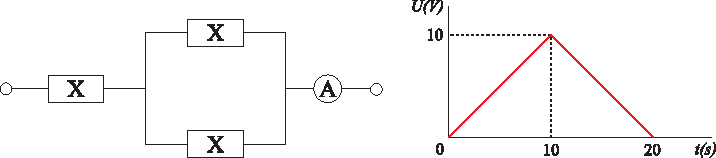
\includegraphics[width=\linewidth]{2009-lahg-03-yl}
\end{center}
\fi
}

% Ü106
\ylDisplay{Must kast} % Ülesande nimi
{Kristian Kuppart} % Autor
{lõppvoor} % Voor
{2013} % Aasta
{G 4} % Ülesande nr.
{4} % Raskustase
{
% Teema: Elektriahelad
\ifStatement
\begin{wrapfigure}{r}{0.35\textwidth}%
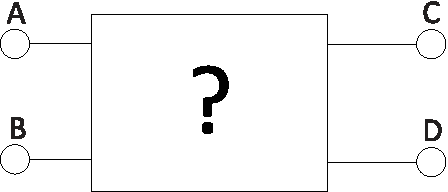
\includegraphics[width=\linewidth]{2013-v3g-04-pilt1}%
\end{wrapfigure}
Joonisel näidatud musta kasti kõik klemmid ühendatakse korraks kokku.
Seejärel, kui klemmide A ja B külge ühendada patarei
pingega $U$ ja klemmide C ja D külge voltmeeter, on voltmeetri näit alghetkel
$U$. Mõõtmise järel ühendatakse kõik klemmid veel korraks kokku.
Kui ühendada sama patarei klemmide C ja D külge ning voltmeeter
klemmide A ja B külge, on voltmeetri näit alghetkel~$\frac{U}{2}.$
Teades, et mustas kastis on ainult identsed kondensaatorid, joonistage musta kasti skeem.
\fi
}

% Ü107
\ylDisplay{Elektroonikaskeem} % Ülesande nimi
{Sandra Schumann} % Autor
{lahtine} % Voor
{2017} % Aasta
{G 4} % Ülesande nr.
{4} % Raskustase
{
% Teema: Elektriahelad
\ifStatement
\begin{wrapfigure}[5]{r}{0.57\textwidth}
	\vspace{-23pt}
	\begin{circuitikz} \draw
		(0.4,0.3) node {A}
		(-0.3,0.6) node {B}
		(-0.3,-0.6) node {C}
		(0,0) node[spdt, xscale=-1] (Sw) {}
		(Sw.out 1) -- (-1.5,0.31)
		(Sw.out 2) -- (-0.59, -1.5) -- (-1.5, -1.5)
		to[american voltage source, l=$9V$] (-1.5,0.31)
		(Sw.in) to[resistor, l=$R$] (3,0) -- (4,0) node[ocirc] {}
		(4.3,0) node {+}
		(4.3,-1.5) node {-}
		(4,-1.5) node[ocirc] {} -- (-0.59, -1.5)
		(3,-1.5) to[capacitor] (3,0)
		;
	\end{circuitikz}
\end{wrapfigure}

Joonisel on antud teatud elektroonikaseadme ühe osa skeem, mis koosneb \SI{9}{\volt} vooluallikast, takistist ja kondensaatorist koosnevast filtrist, väljundklemmidest ja lülitist. Lüliti kaks võimalikku asendit on \enquote{sees} (ühendatud on A ja B) ning \enquote{väljas} (ühendatud on A ja C). Antud olukorras ei ole väljundklemmide külge midagi ühendatud.

Kui toodud skeemis viia lüliti asendist \enquote{sees} asendisse \enquote{väljas} (st lülitada seade välja) ja muuta seejärel vooluallika polaarsus vastupidiseks, siis töötab elektroonikaseade pärast sisselülitamist endiselt. Kui aga vooluallika polaarsust muuta ilma seadet välja lülitamata, siis põleb takisti $R$ läbi. Eeldusel, et takisti põleb läbi niipea, kui sellel eralduv võimsus ületab \SI{0.25}{\watt}, leia $R$ minimaalne ja maksimaalne võimalik väärtus.
\fi
}

% Ü108
\ylDisplay{Takisti} % Ülesande nimi
{Jaan Kalda} % Autor
{piirkonnavoor} % Voor
{2007} % Aasta
{G 7} % Ülesande nr.
{5} % Raskustase
{
% Teema: Elektriahelad
\ifStatement
Oletagem, et me tahame teha takisti takistusega $R = 1 \ohm$, mille takistuse temperatuurisõltuvus oleks toatemperatuuri ümbruses võimalikult väike. Olgu meil kasutada raudtraat ristlõikepindalaga $s = \SI{0,030}{mm^2}$ ja grafiitpulk ristlõikepindalaga $S = \SI{3,0}{mm^2}$. Kuidas valmistada soovitud takistit ja kui pikki grafiitpulga ning terastraadi juppe tuleb seejuures kasutada? Grafiidi ja raua eritakistused on vastavalt $\rho_g = \SI{3,0e5}{\ohm.m}$ ning $\rho_r = \SI{9,7e-8}{\ohm.m}$; takistuse temperatuurikoefitsiendid (suhtelised muutused $\Delta R/R$ temperatuuri kasvamisel ühe kraadi võrra) on $\alpha_g = \SI{-5,0e-3}{K^{-1}}$ ning $\alpha_r = \SI{6,41e-3}{K^{-1}}$
\fi
}

% Ü109
\ylDisplay{Kondensaatoriredel} % Ülesande nimi
{Siim Ainsaar} % Autor
{piirkonnavoor} % Voor
{2007} % Aasta
{G 8} % Ülesande nr.
{5} % Raskustase
{
% Teema: Elektriahelad
\ifStatement
Ühesugustest kondensaatoritest mahtuvusega $C$ on koostatud joonisel näidatud lõpmatu ahel. Leidke ahela kogumahtuvus $C_k$.

\begin{center}
	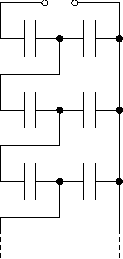
\includegraphics[width=0.3\linewidth]{2007-v2g-08-yl}
\end{center}
\fi
}

% Ü110
\ylDisplay{Traat} % Ülesande nimi
{Jaan Kalda} % Autor
{lõppvoor} % Voor
{2008} % Aasta
{G 7} % Ülesande nr.
{5} % Raskustase
{
% Teema: Elektriahelad
\ifStatement
Ühtlase ristlõikega traati (ristlõike pindala $S = \SI{1}{mm^2}$) venitati nii, et tema erinevad lõigud venisid erinevalt. Enne venitamist oli traadile märgitud jooned iga millimeetri tagant. Joonisel on toodud nende joonte vahekaugused $\Delta$ pärast venitamist sõltuvuses kaugusest traadi ühest otsast $l$ ($l$ on mõõdetud pärast venitamist). Leidke selle nüüdseks 4 meetri pikkuse traadi takistus, arvestades, et traadi materjali tihedus ja eritakistus $\rho = \SI{1e-6}{\ohm.m}$ venitamise tagajärjel ei muutunud.

\begin{center}
	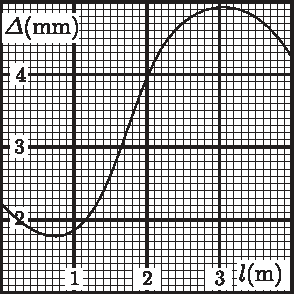
\includegraphics[width=0.6\linewidth]{2008-v3g-07-yl}
\end{center}
\fi
}

% Ü111
\ylDisplay{Kondensaator} % Ülesande nimi
{Aigar Vaigu} % Autor
{piirkonnavoor} % Voor
{2010} % Aasta
{G 7} % Ülesande nr.
{5} % Raskustase
{
% Teema: Elektriahelad
\ifStatement
Muudetava mahtuvusega kondensaator on ühendatud patareiga,
mille klemmide pinge on $U$. Kondensaatori mahtuvust muudetakse laadimisel nii, et
kondensaatori laadimise vool $I$ on konstantne. Leidke patarei võimsus ja kondensaatori laadimisel energia salvestamise kiirus.
Põhjendage võimalikku erinevust.
\fi
}

% Ü112
\ylDisplay{Elektriline sild} % Ülesande nimi
{Jaan Kalda} % Autor
{lõppvoor} % Voor
{2012} % Aasta
{G 3} % Ülesande nr.
{5} % Raskustase
{
% Teema: Elektriahelad
\ifStatement
Joonisel toodud skeemis on tegemist ühesuguste takistitega takistustega $R_1 = R_2 = R_3 = R_4 = R$ ning ühesuguste
ideaalsete patareidega elektromotoorjõududega ${\cal E}_1 = {\cal E}_2
= {\cal E}$. Leidke voolutugevused takistites (st $I_1$, $I_2$, $I_3$ ja
$I_4$ avaldised suuruste $R$ ja ${\cal E}$ kaudu).

\begin{center}
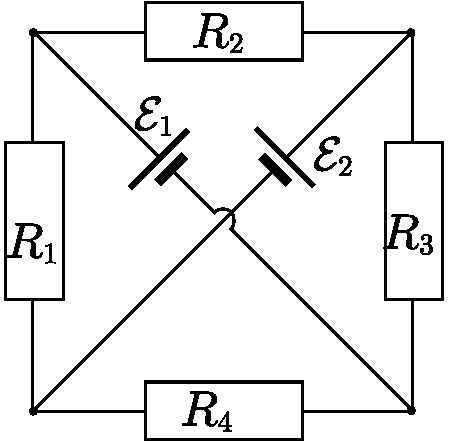
\includegraphics[width=0.35\linewidth]{2012-v3g-03-elektriline_sild}%
\end{center}
\fi
}

% Ü113
\ylDisplay{Must kast} % Ülesande nimi
{Jaan Kalda} % Autor
{lõppvoor} % Voor
{2015} % Aasta
{G 4} % Ülesande nr.
{5} % Raskustase
{
% Teema: Elektriahelad
\ifStatement
Mustas kastis on kolmest takistist ja ideaalsest ampermeetrist koosnev skeem. Lisaks on mustal kastil kolm väljundklemmi $A$, $B$ ja $C$. Kui rakendada pinge $U=\SI{12}{V}$ klemmide $A$ ja $B$ vahele, siis on ampermeetri näit $I_{AB}=\SI{2}{A}$. Klemmide $A$ ja $C$ puhul on lugem $I_{AC}=\SI{4}{A}$ ning klemmide $B$ ja $C$ puhul $I_{BC}=\SI{6}{A}$. Joonistage mustas kastis olev skeem ning märkige sellele takistite takistused.
\fi
}

% Ü114
\ylDisplay{Viisnurk} % Ülesande nimi
{Jaan Kalda} % Autor
{lõppvoor} % Voor
{2017} % Aasta
{G 6} % Ülesande nr.
{5} % Raskustase
{
% Teema: Elektriahelad
\ifStatement
Leidke joonisel toodud skeemis ampermeetri ja voltmeetri näidud. Kõik takistid on takistusega $R=\SI{1}{\ohm}$, pinge patarei klemmidel $U=\SI{7}{\volt}$.

\begin{center}
	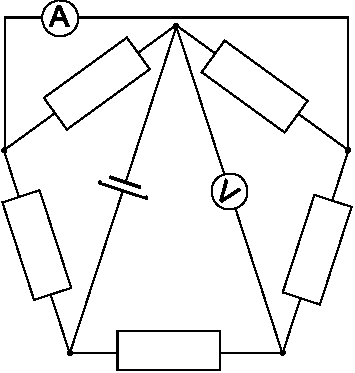
\includegraphics[width=0.4\textwidth]{2017-v3g-06-viisnurk}
\end{center}
\fi
}

% Ü115
\ylDisplay{12 lampi} % Ülesande nimi
{Valter Kiisk} % Autor
{piirkonnavoor} % Voor
{2018} % Aasta
{G 8} % Ülesande nr.
{5} % Raskustase
{
% Teema: Elektriahelad
\ifStatement
Juku käsutuses on 12 ühesugust taskulambipirni ning patarei, mille klemmipinge on täpselt 5 korda suurem pirni nimipingest. Lisaks leidis ta juhtumisi takisti, mille takistus on parajasti pool lambi hõõgniidi takistusest töörežiimis (viimase sai ta teada jagades lambi soklile kirjutatud nimipinge ja -voolu omavahel).\\
\osa Kuidas tuleb ühendada nimetatud komponendid elektriahelasse, et kõik 12 pirni põleksid normaalheledusega?\\
\osa Mitu korda kasvab (või kahaneb) lampide koguvõimsus, kui üks lampidest läbi põleb? Lampide takistuse sõltuvust temperatuurist võib jätta arvestamata.
\fi
}

% Ü116
\ylDisplay{Kondensaatorid} % Ülesande nimi
{Mihkel Rähn} % Autor
{piirkonnavoor} % Voor
{2006} % Aasta
{G 7} % Ülesande nr.
{6} % Raskustase
{
% Teema: Elektriahelad
\ifStatement
\begin{wrapfigure}[9]{r}{0.4\textwidth}
	\begin{center}
		\vspace{-25pt}
		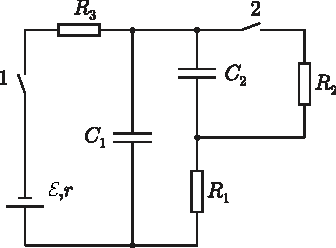
\includegraphics[width=\linewidth]{2006-v2g-07-yl}
	\end{center}
\end{wrapfigure}
Joonisel toodud elektriskeemil on vooluallikas elektromotoorjõuga $\mathcal E$ ja sisetakistusega $r$, kolm takistit takistustega $R_1 = R_2 = R_3 = R$ ning kondensaatorid mahtuvustega $C_1$ ja $C_2$. Arvutage, kui suured on elektrilaengud kondensaatoritel pärast pika aja möödumist, kui:\\
\osa lüliti 1 on suletud, lüliti 2 on avatud;\\
\osa mõlemad lülitid on suletud;\\
\osa eelmisest seisust avatakse mõlemad lülitid üheaegselt. 
\fi
}

% Ü117
\ylDisplay{Kondensaatorid} % Ülesande nimi
{Mihkel Kree} % Autor
{lõppvoor} % Voor
{2009} % Aasta
{G 3} % Ülesande nr.
{6} % Raskustase
{
% Teema: Elektriahelad
\ifStatement
Koosnegu kondensaatorite süsteem viiest kondensaatorist. Alghetkel on kolm neist laenguta ning kahel paikneb laeng $q$ (vt joonist). Missugune laeng koguneb keskmisele kondensaatorile, kui süsteem on jõudnud tasakaaluolekusse?

\begin{center}
	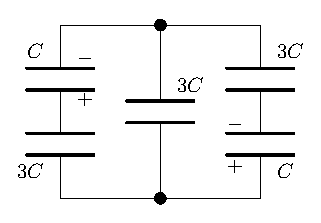
\includegraphics[width=0.42\linewidth]{2009-v3g-03-G_kondensaatorid.eps}
\end{center}
\fi
}

% Ü118
\ylDisplay{Elektriahela energia} % Ülesande nimi
{Eero Vaher} % Autor
{piirkonnavoor} % Voor
{2014} % Aasta
{G 8} % Ülesande nr.
{6} % Raskustase
{
% Teema: Elektriahelad
\ifStatement
Suletud elektriahelas on jadamisi ühendatud takisti takistusega $R=\SI{100}{\ohm}$, kondensaator mahtuvusega $C=\SI{200}{\nano\farad}$, tühise aktiivtakistusega induktiivpool induktiivsusega $L=\SI{10}{\milli\henry}$ ning sobivalt ühendatud ideaalsed mõõteseadmed. Hetkel $t_0$ mõõdeti voolutugevuseks läbi kondensaatori $I=\SI{300}{\milli\ampere}$ ning pingeks poolil $U=\SI{50}{\volt}$. Teada on, et mõõtmise hetkel on vool poolis suunatud kõrgema potentsiaaliga piirkonnast madalama potentsiaaliga piirkonda. Kas mõõtmise hetkel $t_0$ oli rohkem energiat poolil või kondensaatoril? 
\fi
}

% Ü119
\ylDisplay{Vooluallikad} % Ülesande nimi
{Sandra Schumann} % Autor
{lõppvoor} % Voor
{2016} % Aasta
{G 7} % Ülesande nr.
{6} % Raskustase
{
% Teema: Elektriahelad
\ifStatement
Vaatleme joonisel näidatud elektriskeemi, kus noolega tähistatud skeemielement on konstantse voolu allikas voolutugevusega $I=\SI{2}{mA}$ noolega tähistatud suunas. Leidke pinge $U$ väljundklemmidel ja voolutugevus läbi takisti $R=\SI{10}{k\ohm}$ kahe juhu jaoks: $\textbf{a)}$ kui lüliti K on suletud ja $\textbf{b)}$ kui lüliti on avatud.

\begin{center}
	\begin{circuitikz}[american voltages] \draw
		(0,0) to[battery1, l=\SI{1}{V}] (0,1.5)
		to[american current source, l=\SI{2}{mA}] (0,3) --(0,4)
		to[european resistor, l=\SI{10}{k\ohm}, *-] (2,4)
		to[battery1, l=\SI{2}{V}] (4,4)
		to[european resistor, l_=\SI{5}{k\ohm}, *-] (4,0) -- (5,0)
		to[battery1, l_=\SI{3}{V}] (5,4) -- (4,4)
		(4,0) to[short, *-*] (0,0)
		(0, 1.3) to[short,*-] (1.2, 1.3) -- (1.2, 2.05);\draw[thick] (1.2, 2.05) -- +(60:0.5) ;
		\draw (1.2,2.55) -- (1.2,3.3) to[short,-*] (0,3.3)
		(0,4) to[short, -*] (-2,4)
		to [open, v_<=$U$] (-2,0)
		to[short, *-] (0,0)
		
		(1.5, 2.2) node[right] {K};
	\end{circuitikz}
\end{center}
\fi
}

% Ü120
\ylDisplay{Takistuste tuvastamine} % Ülesande nimi
{Eero Vaher} % Autor
{lõppvoor} % Voor
{2018} % Aasta
{G 7} % Ülesande nr.
{6} % Raskustase
{
% Teema: Elektriahelad
\ifStatement
\begin{wrapfigure}[10]{r}{0.4\textwidth}
\vspace{-20pt}
\begin{resizebox}{\linewidth}{!}{
\begin{circuitikz}
\draw
(1,0) to[battery1,l_=${U_0=\SI{14}{V},\,I_0=\SI{10}{A}}$] (8,0) to (1,0) to (1,2.5) to (2,2.5) to[short, *-] (2,4) to[resistor,l=${R_1}$, -*] (4.5,4) to[resistor,l=${R_4}$] (7,4) to[short, -*] (7,2.5) to (8,2.5) to (8,0)
(2,2.5) to (2,1) to[resistor,l=${R_2}$, -*] (4.5,1) to[resistor,l=${R_5}$] (7,1) to (7,2.5)
(4.5,1) to[resistor,l_=$R_3$] (4.5,4)
;
\draw[->,thick] (4,2) -- (4,3);
\end{circuitikz}}
\end{resizebox}
\end{wrapfigure}

Vooluallikaga on ühendatud viis takistit. Neist kolme takistus on \SI{1}{\ohm}, ülejäänud kaks on tundmatu, kuid ühesuguse takistusega. Vooluallika pinge $U_0=\SI{14}{V}$ ning voolutugevus selles $I_0=\SI{10}{A}$. Pinge ja voolutugevus kolmandal takistil on vastavalt $U_3=\SI{2}{V}$ ning $I_3=\SI{2}{A}$. Joonisel on märgitud elektrivoolu suund takistis $R_3$. Määrake kõigi takistite takistused.
\fi
}

% Ü121
\ylDisplay{Aku laadimine} % Ülesande nimi
{Valter Kiisk} % Autor
{piirkonnavoor} % Voor
{2008} % Aasta
{G 8} % Ülesande nr.
{7} % Raskustase
{
% Teema: Elektriahelad
\ifStatement
Teatava akumulaatori elektromotoorjõud kasvab laadimise käigus nõnda, nagu kujutatud joonisel. Samas on toodud ka elektriskeem, mida Juku kavatseb kasutada sellise akumulaatori laadimiseks. Pingeallika klemmidel on pinge \SI{6}{V}. Nii pingeallika kui ka aku sisetakistust võib lugeda tühiseks. Kuidas peaks Juku valima takistite $R_1$ ja $R_2$ väärtused, kui ta taotleb, et maksimaalne laadimisvool ei ületaks \SI{100}{mA} ja laadimisvool muutuks nulliks, kui akumulaator on täielikult laetud? 

\begin{center}
	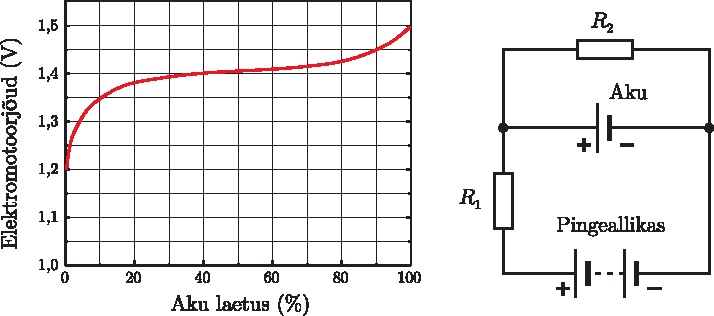
\includegraphics[width=\linewidth]{2008-v2g-08-yl}
\end{center}
\fi
}

% Ü122
\ylDisplay{Raudtee} % Ülesande nimi
{Mihkel Pajusalu} % Autor
{piirkonnavoor} % Voor
{2012} % Aasta
{G 8} % Ülesande nr.
{7} % Raskustase
{
% Teema: Elektriahelad
\ifStatement
\begin{wrapfigure}{r}{18mm}%
\vspace{-15pt}
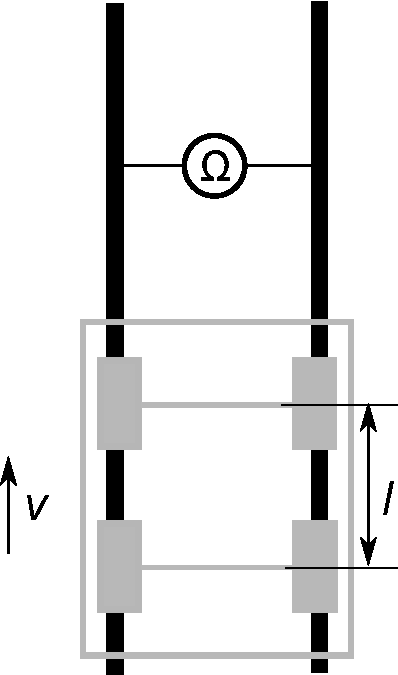
\includegraphics[width=\linewidth]{2012-v2g-08-rong}%
\end{wrapfigure}
Mõõdame raudteel elektritakistust kahe kõrvutise rööpa vahel nii, nagu joonisel.
Rööbastel sõidab vagun kiirusega $v$. Olgu vagunil kaks rattapaari,
mille vahekaugus on $l$. Joonistage graafik takistuse muutumisest ajas alates
hetkest, kui vaguni esimene rattapaar on mõõtepunkti ees sellest kaugusel $l/2$, kuni
ajani, kui tagumine rattapaar on mõõtepunkti taga sellest kaugusel $l/2$. Mõlema rattapaari
takistuseks olgu $r$ ja rööpa takistus pikkusühiku kohta $\rho$.
\fi
}

% Ü123
\ylDisplay{Lambid} % Ülesande nimi
{Mihkel Kree} % Autor
{lahtine} % Voor
{2013} % Aasta
{G 9} % Ülesande nr.
{7} % Raskustase
{
% Teema: Elektriahelad
\ifStatement
Juku ehitas kodus niisuguse elektriskeemi nagu joonisel näidatud, kasutades
selleks kuut ühesugust takistit takistusega $R=\SI{10}{\ohm}$, nelja
ühesugust lampi takistusega $r=\SI{20}{\ohm}$ ning pingeallikat
elektromotoorjõuga
$\mathcal{E}=\SI{5}{\volt}$. Arvutage igas lambis (joonisel tähised 1, 2, 3,
4) eralduv võimsus. Pingeallika sisetakistusega mitte arvestada.
\begin{center}
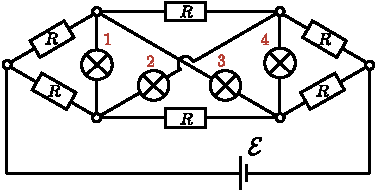
\includegraphics[width=0.6\linewidth]{2013-lahg-09-lambidJoonis-crop}
\end{center}
\fi
}

% Ü124
\ylDisplay{Jõulukaunistus} % Ülesande nimi
{Valter Kiisk} % Autor
{lõppvoor} % Voor
{2010} % Aasta
{G 8} % Ülesande nr.
{8} % Raskustase
{
% Teema: Elektriahelad
\ifStatement
Jõulukaunistuse hankimiseks majandussurutise tingimustes otsustas Juku
ühendada jadamisi kokku 50 valgusdioodi ja toita seda ahelat läbi alaldusdioodi $D$ otse
võrgupingega (vt joonist). Voolu piiramiseks on ahelasse lülitatud takisti
ning voolu pulsatsiooni väljasilumiseks kondensaator. Pinge alaldusdioodil on
tühine, igal valgusdioodil aga $U_d=\SI{3}{V}$. Kui suure takistusega $R$ ja maksimumvõimsusega $N$ tuleks valida
takisti, kui valgusdioodid taluvad voolu kuni $I=\SI{20}{mA}$? Kui suure mahtuvusega $C$
kondensaator kindlustab, et voolutugevuse pulsatsioon jääb $\alpha=\num{5}\%$ piiresse? Võrgupinge
sagedus on $f=\SI{50}{Hz}$ ning amplituudväärtus $U_0=\SI{311}{V}$.

\begin{center}
	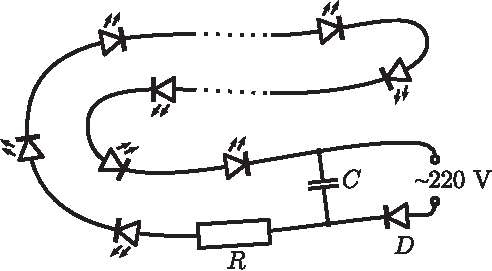
\includegraphics[scale=0.75]{2010-v3g-08-elektrikuunlad2}
\end{center}
\fi
}

% Ü125
\ylDisplay{Dioodid} % Ülesande nimi
{Jaan Kalda} % Autor
{lahtine} % Voor
{2012} % Aasta
{G 8} % Ülesanne nr.
{8} % Raskustase
{
% Teema: Elektriahelad
\ifStatement
\begin{wrapfigure}{r}{0.4\linewidth}
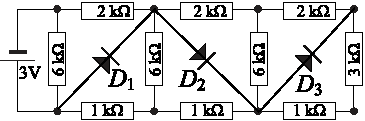
\includegraphics[width=\linewidth]{2012-lahg-08-dioodid}
\end{wrapfigure}
Millised võimsused eralduvad skeemil märgitud dioodidel? Dioodide voolu võib lugeda
nulliks kõikide vastupingete jaoks ning samuti ühest voldist
väiksemate päripingete jaoks; suvalise pärivoolu puhul on dioodi pinge
\SI{1,0}V. Takistite takistused ja elektromotoorjõu väärtus on toodud
joonisel. Dioodi skeemitähise noole suund näitab pärivoolu
suunda.
\fi
}

% Ü126
\ylDisplay{Oktaeeder} % Ülesande nimi
{Jaan Kalda} % Autor
{lahtine} % Voor
{2016} % Aasta
{G 8} % Ülesande nr.
{8} % Raskustase
{
% Teema: Elektriahelad
\ifStatement
Juuresolev skeem kujutab traadist oktaeedrit, iga traadi juurde on kirjutatud selle takistus oomides. 
Ampermeetreid ühendavad traadid on tühiselt väikese takistusega.
Leidke ampermeetrite näidud.

\begin{center}
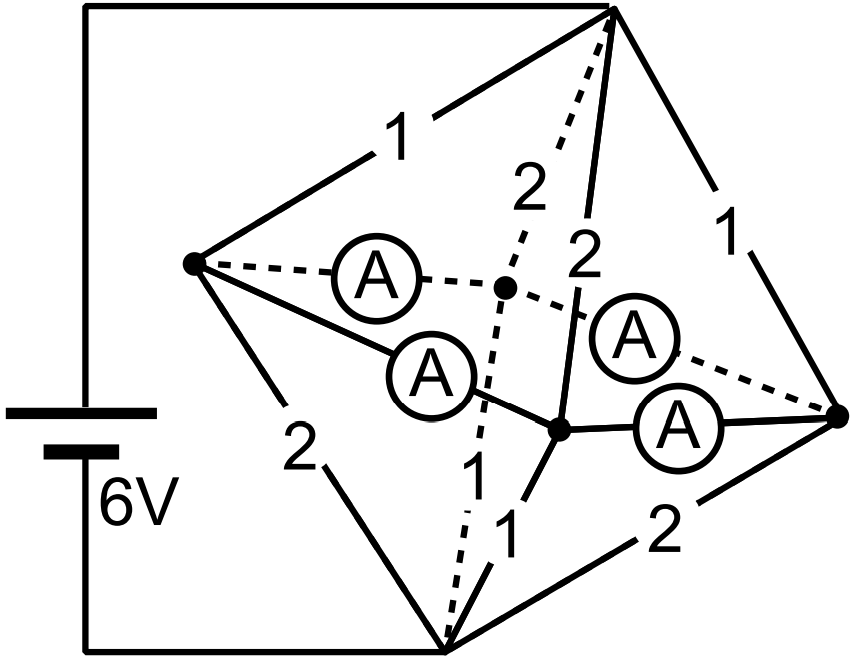
\includegraphics[width=0.5\textwidth]{2016-lahg-08-ampermeeterjoonis.png}
\end{center}
\fi
}

% Ü127
\ylDisplay{Kondensaator} % Ülesande nimi
{Jaan Kalda} % Autor
{lõppvoor} % Voor
{2018} % Aasta
{G 9} % Ülesande nr.
{8} % Raskustase
{
% Teema: Elektriahelad
\ifStatement
\begin{wrapfigure}[7]{r}{0.3\linewidth}
\vspace{-10pt}
\begin{center}
\includegraphics[width=\linewidth]{2018-v3g-09-LC-Q}
\par\end{center} 
\end{wrapfigure}

Vaatleme joonisel kujutatud elektriskeemi, mis koosneb kondensaatorist mahtuvusega $C$, patareist elektromotoorjõuga $\mathcal{E}$, takistist ja hõõglambist, mida võib lugeda mittelineaarseks takistiks (pinge sõltub voolust mittelineaarselt). Algselt oli kondensaator laenguta ja lüliti oli avatud. Seejärel suleti lüliti lühikeseks ajaks, misjärel see avati uuesti ning hoiti lahtisena seni, kuni kondensaator oli täielikult tühjenenud. Selle aja jooksul, mil lüliti oli suletud, eraldus kogu skeemil soojushulk $Q_1$; lüliti avamise järel eraldus täiendavalt veel soojushulk $Q_2$. Leidke laeng, mis läbis hõõglambi sel perioodil, kui lüliti oli suletud.
\fi
}

% Ü128
\ylDisplay{Närvirakk} % Ülesande nimi
{Andres Laan} % Autor
{lõppvoor} % Voor
{2011} % Aasta
{G 9} % Ülesande nr.
{9} % Raskustase
{
% Teema: Elektriahelad
\ifStatement
Närviraku membraani võib vaadelda kui õhukest kilet mahtuvusega $C$, mida läbivad ioonkanalid, mis võimaldavad laengutel liikuda läbi
membraani. Närviraku elektrilise tasakaalu seisukohast on olulisteks ioonideks
naatrium ja kaalium. Kui naatriumioon (laenguga $+e$) läbib ioonkanali (sisenedes närvirakku), siis sooritavad keemilised jõud töö $e\mathcal{E}_{\mathrm{Na}}$, st võib öelda, et
naatriumioonidele mõjub ioonkanalis elektromotoorjõud $\mathcal{E}_{\mathrm{Na}}$. Kaaliumioonide
puhul on kanali läbimise protsess täpselt samasugune, kuid efektiivne elektromotoorjõud on sel puhul $\mathcal{E}_{\mathrm{K}}$ ($\neq \mathcal{E}_{\mathrm{Na}}$). Peale keemiliste jõudude töö toimivad
laengu liikumisel ioonkanalis ka hõõrdejõud, mida saab kirjeldada elektrilise
takistuse abil: naatriumioonide jaoks on membraani elektriline takistus $R_{\mathrm{Na}}$ ja kaaliumioonide jaoks $R_{\mathrm{K}}$. Millise laengu omandab närviraku membraan
elektrilise tasakaalu saabudes? 
\fi
}

% Ü129
\ylDisplay{Türistor} % Ülesande nimi
{Jaan Toots} % Autor
{lõppvoor} % Voor
{2015} % Aasta
{G 10} % Ülesande nr.
{10} % Raskustase
{
% Teema: Elektriahelad
\ifStatement
\begin{wrapfigure}{r}{0.48\textwidth}
\begin{circuitikz} \draw

(0,2) to[resistor=$R$] (2,2)
 to[Do,l=$T_1$, *-*] (2,0) -- (0,0)
 to[battery1,l=$U$] (0,2)
(2,2) to[switch] (4,2)
 to[Do,l=$T_2$] (4,0) -- (2,0)
;
\end{circuitikz}
\end{wrapfigure}
Türistori (dioodisarnase elemendi) volt-amper karakteristik on juuresoleval graafikul. Kaks sellist türistori on ühendatud pingeallika ja takistiga kõrvalolevasse skeemi. Takistus $R = \SI{2}{\kilo\ohm}$.\\
{\bf a}) Alguses on lüliti avatud. Pingeallika pinget suurendatakse lineaarselt $t=\SI{42}{\second}$ jooksul väärtuselt $U_0=\SI{0}{\volt}$ kuni väärtuseni $U_a = \SI{42}{\volt}$. Skitseerige ahelat läbiva voolutugevuse $I(t)$ sõltuvus ajast. Milline on voolutugevuse lõppväärtus $I_a$?\\
{\bf b}) Leidke lõppvoolutugevused mõlemas türistoris, kui lüliti suletakse ilma ahelale rakendatud pinget $U_a$ muutmata.

\begin{figure}[h]
\begin{center}
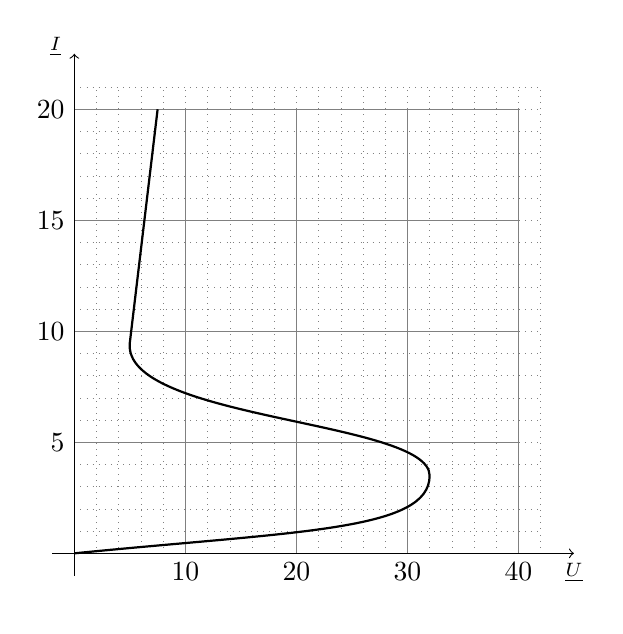
\begin{tikzpicture}[scale=1.41,
axes/.style=]

\draw[step=0.2, gray, dotted, very thin] (0,0) grid (4.2,4.2);
\draw[step=1, gray, very thin] (0,0) grid (4,4);

\begin{scope}[axes]
 \draw[->] (-0.2,0) -- (4.5,0) node[right, below] {$\frac{U}{\si{\volt}}$} coordinate(x axis);
 \draw[->] (0,-0.2) -- (0,4.5) node[above, left] {$\frac{I}{\si{\milli\ampere}}$} coordinate(y axis);

 \foreach \x/\xtext in {1/10, 2/20, 3/30, 4/40}
 \draw (\x,0) node[below] {$\xtext$};
 
 \foreach \y/\ytext in {1/5, 2/10, 3/15, 4/20}
 \draw (0,\y) node[left] {$\ytext$};
\end{scope}

\draw[thick] (0,0) .. controls (2,0.2) and (3.2,0.2) .. (3.2,0.7) .. controls (3.2,1.2) and (5/12,1.2) .. (0.5,1.9) -- (0.75,4);

\end{tikzpicture}

\end{center}
\end{figure}
\fi
}
\newpage\subsection{\protect\StrSubstitute{Elektrostaatika}{-}{ }}

% Ü130
\ylDisplay{Kondensaator} % Ülesande nimi
{Madis Ollikainen} % Autor
{lahtine} % Voor
{2012} % Aasta
{G 3} % Ülesanne nr.
{2} % Raskustase
{
% Teema: Elektrostaatika
\ifStatement
Füüsikatudeng leidis vanade demonstratsioonideks mõeldud eksperimentaalseadmete
hulgast ühe plaatkondensaatori. Noore füüsikuna tundis ta kohe hirmsat soovi
sellega veidi mängida. Ta mõõtis kondensaatori plaatide vahekauguseks $d$
ning seejärel laadis kondensaatori pingeni $U$. Nüüd asetas ta
kondensaatori plaatide vahele ühe kuulikese, mis kukkus alumise plaadi peale
ja siis hakkas uuesti ülespoole tõusma. Kuulikesel kulus alumiselt plaadilt
ülemiseni jõudmiseks aeg $t$. Leidke kuulikese massi ja alumiselt plaadilt
saadud laengu suhe.
\fi
}

% Ü131
\ylDisplay{Juhe} % Ülesande nimi
{Tundmatu autor} % Autor
{lahtine} % Voor
{2005} % Aasta
{G 5} % Ülesande nr.
{3} % Raskustase
{
% Teema: Elektrostaatika
\ifStatement
Sirgjooneline juhe asub sügaval maa all ühtlases pinnases. Lekkevool ühikulise pikkusega juhtmest on $i$. Leidke lekkevoolu tihedus (\si{A/m^2}) kaugusel $r$ juhtmest. Juhtme pikkus on palju suurem kui $r$. Lekkevool on konstantne piki juhet.

\emph{Märkus}. Lekkevooluks nimetatakse voolu, mis levib isolaatorites. 
\fi
}

% Ü132
\ylDisplay{Kuulikesed} % Ülesande nimi
{Tundmatu autor} % Autor
{lahtine} % Voor
{2005} % Aasta
{G 4} % Ülesande nr.
{4} % Raskustase
{
% Teema: Elektrostaatika
\ifStatement
Seitse ühesugust laetud kuulikest laenguga $q$ on seotud omavahel samast materjalist võrdse algpikkusega elastsete niitidega ja saavad liikuda vaid ühes fikseeritud tasapinnas (vt joonist). Vahemaa kahe suvalise naaberkuulikese vahel tasakaalu olekus on $l$. Leidke tõmbepinged niitides.

\begin{center}
	\includegraphics[width=0.35\linewidth]{2005-lahg-04-yl}
\end{center}
\fi
}

% Ü133
\ylDisplay{Tolmukübe} % Ülesande nimi
{Aigar Vaigu} % Autor
{piirkonnavoor} % Voor
{2006} % Aasta
{G 8} % Ülesande nr.
{4} % Raskustase
{
% Teema: Elektrostaatika
\ifStatement
Tolmukübe massiga $m = \SI{1e-9}{g}$ on kondensaatori horisontaalsete plaatide vahel tasakaalus. Laengu pindtihedus kondensaatori plaatidel $\sigma = \SI{2,6e-5}{C/m^2}$. Kui suur on tolmukübeme elektrilaeng? Millise kiirendusega hakkaks tolmukübe langema, kui kondensaatori polaarsus muuta vastupidiseks? Eeldada, et elektriväli kondensaatori plaatide vahel on homogeenne. Õhutakistust mitte arvestada. Elektriline konstant $\varepsilon_0 = \SI{8,85e-12}{F/m}$, õhu dielektriline läbitavus $\varepsilon \approx 1$.
\fi
}

% Ü134
\ylDisplay{Kuulikesed} % Ülesande nimi
{Tundmatu autor} % Autor
{lahtine} % Voor
{2007} % Aasta
{G 7} % Ülesande nr.
{4} % Raskustase
{
% Teema: Elektrostaatika
\ifStatement
Kaks ühesugust kuulikest, millest kumbki kannab laengut $q$, asuvad vertikaalsihis kaugusel $H$ üksteisest. Alumine kuulike on jäigalt kinnitatud, ülemine aga hakkab liikuma vertikaalselt alla suunatud algkiirusega $v$. Kui suur on minimaalne kaugus $h$ alumise kuulikeseni, millele suudab läheneda ülemine kuulike? Ülemise kuulikese mass on $m$. Raskuskiirendus on $g$.
\fi
}

% Ü135
\ylDisplay{Laetud rõngas} % Ülesande nimi
{Tundmatu autor} % Autor
{lahtine} % Voor
{2009} % Aasta
{G 4} % Ülesande nr.
{4} % Raskustase
{
% Teema: Elektrostaatika
\ifStatement
Peenikesest traadist rõngas raadiusega $R$ on ühtlaselt laetud negatiivse laenguga $Q$. Elektron massiga $m$ ja laenguga $e$ läheneb rõngale mööda sirget, mis on risti rõnga tasandiga ning läbib rõnga keskpunkti. Millist tingimust peab rahuldama elektroni kiirus punktis, mis asub kaugusel $d = R\sqrt 3$ rõnga keskpunktist, et elektron saaks rõngast läbi lennata?
\fi
}

% Ü136
\ylDisplay{Ioonmootor} % Ülesande nimi
{Mihkel Pajusalu} % Autor
{lahtine} % Voor
{2010} % Aasta
{G 6} % Ülesande nr.
{4} % Raskustase
{
% Teema: Elektrostaatika
\ifStatement
Kosmosesond on varustatud lihtsa ioonmootoriga, mis koosneb ksenooni
ioonide $\mathrm{Xe}^+$ allikast ja kahest elektroodist, mille vahele rakendatakse pinge
$U$ ja mille vahelist maad läbides ioone kiirendatakse. Kui suurt kogust
(mass) ksenooni on vaja, et selle mootoriga sondi kiirust tõsta
$\Delta v=\SI{1}{km/s}$ võrra?
%
Ksenooni aatommass $\mu=\SI{131,29}{g/mol}$, kosmosesondi mass $M=\SI{1000}{kg}$, kiirendav pinge
$U=\SI{100}{kV}$, elementaarlaeng $e=\SI{1,60 e-19}{C}$, Avogadro arv
$N_A= \SI{6,02 e23}{mol^{-1}}$.
\fi
}

% Ü137
\ylDisplay{Elektron} % Ülesande nimi
{Mihkel Kree} % Autor
{lahtine} % Voor
{2017} % Aasta
{G 3} % Ülesande nr.
{4} % Raskustase
{
% Teema: Elektrostaatika
\ifStatement
\begin{wrapfigure}[7]{r}{0.5\linewidth}
	\vspace{-10pt}
	\hspace{-10pt}
	\includegraphics[width=\linewidth]{2017-lahg-03-elJoonisMK.pdf}
\end{wrapfigure}

Elektron liigub vaakumis ning siseneb paralleelsete plaatide vahel paiknevasse ruumipiirkonda selle ülemisest servast nii, et elektroni kiirusvektor on paralleelne plaatidega (vt joonist). Kui suur on elektroni minimaalne võimalik kiirus $v_\mathrm{min}$ plaatide vahelisest ruumipiirkonnast väljumisel? Plaatide pikkus on $l$ ja nende vahekaugus $d$. Plaatide vahel on ühtlane elektriväli $\vec{E}$ ning ääreefektidega pole vaja arvestada. Elektroni laeng on $q$ ning mass $m$. Gravitatsioonijõuga pole vaja arvestada.
\fi
}

% Ü138
\ylDisplay{Lendav elektronkahur} % Ülesande nimi
{Siim Ainsaar} % Autor
{lõppvoor} % Voor
{2006} % Aasta
{G 6} % Ülesande nr.
{5} % Raskustase
{
% Teema: Elektrostaatika
\ifStatement
Jaan Tatikal tuli järjekordne lennumasinaidee, mida ta kohe realiseerima tõttas. Ta nimelt ehitas palkidest platvormi, mille alla kinnitas telerist välja lõhutud elektronkahuri koos vajaliku elektroonika ja akuga. Elektrone kiirendav pinge on $U$, voolutugevus elektronkiires $I$. Leidke, kui suurt tõstejõudu $F$ suudab see seade tekitada. Missugust tingimust peaksid $U$ ja $I$ rahuldama, et taoline lennumasin suudaks leiduri õhku tõsta? Kas see on ka realistlik (televiisorites $U \approx \SI{30}{kV}$, $I \approx \SI{100}{\micro A}$)? Relativistlikke efekte pole vaja arvestada; elektroni algkiirus katoodi juures on 0. Eeldage, et kiir üldse moodustub (õhu olemasoluga ärge arvestage). Tatika mass koos platvormi ja seadmega on $m_T \approx \SI{150}{kg}$, raskuskiirendus $g \approx \SI{9,8}{m/s^2}$. Elektroni laengu ja massi suhe $k = e/m_e \approx \SI{1,76e11}{C/kg}$.
\fi
}

% Ü139
\ylDisplay{Elektronkiir} % Ülesande nimi
{Tundmatu autor} % Autor
{lahtine} % Voor
{2008} % Aasta
{G 7} % Ülesande nr.
{5} % Raskustase
{
% Teema: Elektrostaatika
\ifStatement
Kitsas elektronkiir läbib vaakumis tasaparalleelsete plaatide vahelise pilu ja langeb seejärel fluorestseeruvale ekraanile, mis asub plaatide ekraanipoolsemast servast kaugusel $l = \SI{15}{cm}$. Kui plaatidele antakse pinge $U = \SI{50}{V}$, nihkub helendav punkt ekraanil endisest asukohast kaugusele $s = \SI{21}{mm}$. Plaatidevaheline kaugus $d = \SI{18}{mm}$, plaatide mõõtmed elektronide liikumise suunas on $b = \SI{6}{cm}$. Milline on elektronide algkiirus plaatide vahele sattumisel? Elektroni laengu ja massi suhe $e/m \approx \SI{1,76e11}{C/kg}$.
\fi
}

% Ü140
\ylDisplay{Kuup} % Ülesande nimi
{Jaan Kalda} % Autor
{piirkonnavoor} % Voor
{2008} % Aasta
{G 7} % Ülesande nr.
{5} % Raskustase
{
% Teema: Elektrostaatika
\ifStatement
Õhukesest elektrit mittejuhtivast materjalist on valmistatud kuup küljepikkusega $a$. Kuubil on elektrilaeng ühtlase pindtihedusega $\sigma$ (pindtihedus on laeng pinnaühiku kohta). Ühe tahu keskkohta lõigatakse väike ruudukujuline auk mõõtmetega $b \times b$ ($b \ll a$). Leida elektrivälja tugevus kuubi keskpunktis.
\fi
}

% Ü141
\ylDisplay{Liikuv laeng} % Ülesande nimi
{Jaan Kalda} % Autor
{piirkonnavoor} % Voor
{2009} % Aasta
{G 6} % Ülesande nr.
{6} % Raskustase
{
% Teema: Elektrostaatika
\ifStatement
Laetud osake laengu ja massi suhtega $q/m = \SI{1}{C/kg}$ seisab algselt paigal. Seejärel hakkab ta liikuma $x$- ja $y$-telje sihis
toimivate elektrivälja impulsside mõjul. Elektrivälja vastavate komponentide $E_x$ ja $E_y$ sõltuvus ajast on toodud graafikul (graafiku mastaap
ei ole korrektne, juhenduda tuleb graafikul näidatud numbritest impulsi
kestvuse $\tau = \SI{1}{ms}$ ja amplituudi $E_0 = \SI{1}{kV/m}$ ning perioodi $T = \SI{2}{s}$
jaoks). Visandage osakese trajektoor ja leidke keskmine kiirus (visandi tegemisel ja arvutustes võib lugeda ajavahemiku $\tau = \SI{1}{ms}$ jooksul
toimuvad muutused hetkelisteks). 

\begin{center}
	\includegraphics[width=0.6\linewidth]{2009-v2g-06-yl}
\end{center}
\fi
}

% Ü142
\ylDisplay{Sfäärid} % Ülesande nimi
{Kristian Kuppart} % Autor
{lahtine} % Voor
{2011} % Aasta
{G 8} % Ülesande nr.
{6} % Raskustase
{
% Teema: Elektrostaatika
\ifStatement
Kaks juhtivast materjalist sfääri raadiustega $R_1$ ja $R_2$ on ühendatud pika 
juhtmega. Ühele sfääridest antakse mingi laeng. Leidke suhe $\frac{E_1}{E_2}$, kus
$E_1$ ja $E_2$ on elektrivälja tugevused vastavate sfääride pinnal. Eeldage, et
juhtme mahtuvus on tühine ning juhtme pikkus on oluliselt suurem sfääride
raadiustest.
\fi
}

% Ü143
\ylDisplay{Laengud} % Ülesande nimi
{Mihkel Kree} % Autor
{piirkonnavoor} % Voor
{2017} % Aasta
{G 9} % Ülesande nr.
{6} % Raskustase
{
% Teema: Elektrostaatika
\ifStatement
\begin{wrapfigure}{r}{0.3\textwidth}
	\vspace{-25pt}
	\begin{center}
		\includegraphics[width=0.32\textwidth]{2017-v2g-09-laengudjoonis.pdf}
	\end{center}
	\vspace{-10pt}
\end{wrapfigure}

Kaks kera, kumbki laenguga $Q$, on liikumatult fikseeritud nii, et nende keskpunktide kaugus on $2d$. Täpselt nende kerade keskele paigutatakse kolmas kera laenguga $-q$ ning massiga $m$, mis saab liikuda ainult mööda $y$-telge (vt joonis). Leidke selle kolmanda kera väikeste $y$-suunaliste võnkumiste periood $T$.
\fi
}

% Ü144
\ylDisplay{Kondensaatorid} % Ülesande nimi
{Oleg Košik} % Autor
{lõppvoor} % Voor
{2005} % Aasta
{G 8} % Ülesande nr.
{7} % Raskustase
{
% Teema: Elektrostaatika
\ifStatement
Kondensaatorid mahtuvustega $2C$ ja $3C$ on ühendatud pingeallikaga, mille pinge on $U$. Osake massiga m ning laenguga $q$ lendab algkiirusega $v$, mis on suunatud paralleelselt kondensaatorite plaatidega (vt joonist). Osake lendab mõlema kondensaatori plaatide vahelt läbi. Mõlema kondensaatori plaatide pikkus on $l$ ning plaatide vahelised kaugused on vastavalt $2d$ ja $d$. Leidke nurk, mille võrra kaldub osake võrreldes esialgse trajektooriga, kui ta väljub joonisel ülemisest kondensaatorist. Eeldada, et see nurk on väike.

\begin{center}
	\includegraphics[width=0.6\linewidth]{2005-v3g-08-yl}
\end{center}
\fi
}

% Ü145
\ylDisplay{Kärbes} % Ülesande nimi
{Stanislav Zavjalov} % Autor
{lahtine} % Voor
{2010} % Aasta
{G 7} % Ülesande nr.
{7} % Raskustase
{
% Teema: Elektrostaatika
\ifStatement
Kärbes on otsustanud
lennates püsida ainult ekvipotentsiaalsete pindade peal. Ta lendab sisse ruumi,
mis on täidetud homogeense elektriväljaga $\vec{E}$, välja jõujoontega risti.
Elektriväljas hoitakse paigal ka laengut $-Q$ nii, et kärbse
trajektoori esialgse puutuja ja laengu vahemaa on $d$ (vt. joonist; $-Q < 0$).
Kui lähedale kärbes laengule jõuab? Eeldage, et $Q \le \pi\epsilon_0Ed^2$.
\begin{center}
	\includegraphics[width=0.4\textwidth]{2010-lahg-07-muha_tekst}
\end{center}
\fi
}

% Ü146
\ylDisplay{Pendel} % Ülesande nimi
{Jonatan Kalmus} % Autor
{lõppvoor} % Voor
{2018} % Aasta
{G 6} % Ülesande nr.
{7} % Raskustase
{
% Teema: Elektrostaatika
\ifStatement
Elektriliselt isoleeritud metallkuul massiga $M$ ja laenguga $Q>0$ ripub vertikaalse vedru otsas jäikusega $k$ tasakaaluasendis gravitatsiooniväljas $g$. Nüüd tekitatakse vertikaalne elektriväli tugevusega $E$, mis on esialgu suunatud alla ning edaspidi alati kuuli liikumise suunas. Eeldada, et elektriväli muutub hetkeliselt. Leida kuuli kaugus algsest asukohast ajahetkel $t=7\pi \sqrt{\frac{M}{k}}$.
\fi
}

% Ü147
\ylDisplay{Laetud klotsid} % Ülesande nimi
{Tundmatu autor} % Autor
{lahtine} % Voor
{2006} % Aasta
{G 9} % Ülesande nr.
{8} % Raskustase
{
% Teema: Elektrostaatika
\ifStatement
Horisontaalsel siledal dielektrilisel pinnal asuvad kaks laetud klotsi massidega $m$ ja samanimeliste laengutega $q$. Alghetkel on vahemaa nende vahel $l$. Mis tingimusel hakkavad klotsid liikuma ja kui suur on vahemaa $L$ nende vahel, kui liikumine lõppeb? Hõõrdetegur klotside ja pinna vahel on $\mu$. Klotside mõõtmeid ja liikuvate laengute elektromagnetkiirgust mitte arvestada. Pinna dielektriline läbitavus on 1.
\fi
}

% Ü148
\ylDisplay{Kosmoseprügi} % Ülesande nimi
{Siim Ainsaar} % Autor
{lõppvoor} % Voor
{2009} % Aasta
{G 9} % Ülesande nr.
{8} % Raskustase
{
% Teema: Elektrostaatika
\ifStatement
Kaks ühesugust elektriliselt laetud
kuuli, mis on ühendatud ideaalse nööriga, hõljuvad vabalt kosmoses. Kummagi
kera laeng on $q$ ja mass $M$, nööri pikkus on $l$.
Ootamatult lendab nööriga risti selle keskkoha pihta kosmoseprügi tükk massiga $m$ ja kiirusega
$v$ ning jääb nööri külge kinni. Millisele vähimale kaugusele $d$ lähenevad teineteisele kuulid?
Eeldada, et kuulikeste diameetrid on väiksemad kui otsitav kaugus $d$.
\fi
}

% Ü149
\ylDisplay{Koonus} % Ülesande nimi
{Stanislav Zavjalov} % Autor
{piirkonnavoor} % Voor
{2012} % Aasta
{G 10} % Ülesande nr.
{8} % Raskustase
{
% Teema: Elektrostaatika
\ifStatement
Ühtlaselt laetud koonus kõrgusega $H$ tekitab oma tipus $S$ potentsiaali
$\varphi_0$. Sellest lõigatakse ära väiksem koonus kõrgusega $h$, mis on suure
koonusega sarnane, kahe koonuse tipud ühtivad. Seejärel eemaldatakse väiksem koonus
lõpmatusesse. Milline on uus potentsiaali väärtus punktis $S$?
\fi
}

% Ü150
\ylDisplay{Laengud} % Ülesande nimi
{Jaan Kalda} % Autor
{lõppvoor} % Voor
{2012} % Aasta
{G 9} % Ülesande nr.
{8} % Raskustase
{
% Teema: Elektrostaatika
\ifStatement
\begin{wrapfigure}{r}{0.33\textwidth}%
\vspace{-10pt}
\includegraphics[width=\linewidth]{2012-v3g-09-laeng}%
\end{wrapfigure}
Positiivselt laetud osake kiirendatakse koordinaatide alguspunktis pinge $4U$ (kus $U>0$) abil teatud kiiruseni, mis
lebab $x-y$ tasandis $30$-kraadise nurga all $x$-telje suhtes, vt joonist. Elektriline potentsiaal $V(x,y)\equiv V(x)$
sõltub ainult $x$-koordinaadist: kui
$3a<x<4a$, siis $V(x)=U$ ning vastasel korral $V(x)=0$; peale elektrostaatilise jõu osakesele mingeid muid jõude ei mõju ning $a>0$.

\osa Visandage laengu trajektoor $x-y$-tasandis (geomeetrilisi mõõtmeid ja nurki pole vaja märkida).

\osa Nüüd on laetud osakeste allikaks koordinaatide alguspunktis asuv koaksiaalne vaakumdiood, mistõttu pinge $4U$
abil kiirendatud osakesi liigub isotroopselt (võrdsel hulgal) kõigis $x-y$-tasandi suundades;
$z$-suunaline kiiruskomponent on kõigil osakestel 0. Milline osa kõigist kiiratud osakestes jõuab ruumipiirkonda $x>4a$?
\fi
}

% Ü151
\ylDisplay{Kondensaator} % Ülesande nimi
{Stanislav Zavjalov} % Autor
{lõppvoor} % Voor
{2013} % Aasta
{G 10} % Ülesande nr.
{8} % Raskustase
{
% Teema: Elektrostaatika
\ifStatement
Ruudukujuliste plaatidega kondensaator plaadi pindalaga~$S$ ning plaatidevahelise
kaugusega $d \ll \sqrt{S}$ on laetud pingeni $U_0$ ning seejärel
patareist lahti ühendatud. Kondensaatori sisse viiakse ruudukujuline juhtiv
plaat, samuti pindalaga $S$ ning paksusega $d/2$, kuni plaat on täielikult
kondensaatori sees. Protsessi jooksul plaat ei puutu kokku
kondensaatori plaatidega ning on nendega paralleelne. Kui palju tööd tehti
plaadi sisseviimisel? Selgitage, kas plaat tõmbus ise sisse või pidid välisjõud
selle sisse lükkama. Servaefekte pole vaja arvesse võtta. Vaakumi dielektriline
läbitavus on $\varepsilon_0$.
\fi
}

% Ü152
\ylDisplay{Kondensaator} % Ülesande nimi
{Jaan Kalda} % Autor
{lahtine} % Voor
{2017} % Aasta
{G 7} % Ülesande nr.
{8} % Raskustase
{
% Teema: Elektrostaatika
\ifStatement
\begin{wrapfigure}[5]{r}{0.35\linewidth}
	\vspace{-13pt}
	\includegraphics[width=\linewidth]{2017-lahg-07-res-cap2.pdf}
\end{wrapfigure}

Plaatkondensaator mahtuvusega $C$ omab plaatidevahelist kaugust $d$. Plaatide vahele asetatakse kaks dielektrilist plaati paksusega $d/2$. Ühe plaadi dielektriline läbitavus on $\varepsilon$, teisel $2\varepsilon$. Milline on nüüd kondensaatori mahtuvus? Milline laeng on plaatide eralduspinnal, kui kondensaatorile rakendatakse pinge $U_0$?
\fi
}

% Ü153
\ylDisplay{Laengutega pulk} % Ülesande nimi
{Jaan Kalda} % Autor
{piirkonnavoor} % Voor
{2015} % Aasta
{G 10} % Ülesande nr.
{9} % Raskustase
{
% Teema: Elektrostaatika
\ifStatement
\osa Dielektrikust pulk massiga $m$ ja pikkusega $L$ kannab kummaski otsas positiivset laengut $q$ (keskosa on laenguta, seega kogulaeng on $2q$). Piirkonnas $x<0$ on $x$-telje sihiline elektriväli tugevusega $E_0$ ja piirkonnas $x>0$ --- sama tugev $x$-teljega antiparalleelne elektriväli. Pulga keskpunt on koordinaatide alguspunktis ja pulk on paralleelne $x$-teljega. Pulgale antakse $x$-telje sihiline algkiirus $v$. Leidke võnkumiste periood. Pulk on paigaldatud nii, et see ei saa pöörelda, vaid üksnes liikuda $x$-telje sihis.

\osa Leidke väikeste võnkumiste periood siis, kui konfiguratsioon on muus osas sama, kuid punktlaengute asemel on kogulaeng $Q$ jaotunud ühtlaselt üle terve pulga.
\fi
}

% Ü154
\ylDisplay{Kuulid} % Ülesande nimi
{Jaan Kalda} % Autor
{lahtine} % Voor
{2016} % Aasta
{G 10} % Ülesande nr.
{9} % Raskustase
{
% Teema: Elektrostaatika
\ifStatement
Kaks metallkuulikest raadiusega $R$ on ühendatud peenikese metalltraadi abil ja asuvad homogeenses 
elektriväljas tugevusega $E$. Metalltraadi pikkus on $l$, kusjuures $l\gg R$. 
Süsteem on tasakaalus. Leidke mehaaniline pinge $T$ traadis.
\fi
}

% Ü155
\ylDisplay{Kaks kuuli} % Ülesande nimi
{Jaan Kalda} % Autor
{lõppvoor} % Voor
{2018} % Aasta
{G 10} % Ülesande nr.
{9} % Raskustase
{
% Teema: Elektrostaatika
\ifStatement
Kaks ühesugust metallkuuli raadiusega $R$ ja massiga $m$ on ühendatud peenikese terastraadiga pikkusega $L\gg R$. Piirkonnas $x\ge 0$ on elektriväli tugevusega $E$, mis on suunatud piki $x$-telge; piirkonnas $x< 0$ elektriväli puudub. Alghetkel on kuulid paigal ja üksteisest kaugusel $L$, nii et traat on pingul ning paralleelne $x$-teljega; ühe kuuli keskpunkt asub punktis $x=R$ ning teine kuul --- piirkonnas $x<0$. Visandage kvalitatiivselt kuulide kiiruse graafik sõltuvuses ajast (kvantitatiivset ajaskaalat ei ole vaja) ning leidke nende kiirus punkti $x=2L$ läbimisel. Terastraadi mahtuvus lugeda tühiselt väikeseks.
\fi
}

% Ü156
\ylDisplay{Kolm kuuli} % Ülesande nimi
{Jaan Kalda} % Autor
{lõppvoor} % Voor
{2016} % Aasta
{G 10} % Ülesande nr.
{10} % Raskustase
{
% Teema: Elektrostaatika
\ifStatement
Kolm väikest kuuli massiga $m$ kannavad ühesuguseid elektrilaenguid $q$ ning on ühendatud isoleerivast materjalist niitide abil võrdhaarseks kolmnurgaks $ABC$, kus $\angle BAC=120^\circ$ ning selle nurga tipus asuva kuuli $A$ vastaskülje niidi pikkus $|BC|=L$. Niit $BC$ lõigatakse katki. Leidke \osa kuuli $A$ maksimaalne kiirus edasise liikumise käigus ning \osa kuulikeste kiirendused vahetult pärast niidi läbi lõikamist. Gravitatsioonilise vastasmõjuga mitte arvestada.
\fi
}
\newpage\subsection{\protect\StrSubstitute{Gaasid}{-}{ }}

% Ü157
\ylDisplay{Jalgpall} % Ülesande nimi
{Tundmatu autor} % Autor
{lahtine} % Voor
{2006} % Aasta
{G 1} % Ülesande nr.
{1} % Raskustase
{
% Teema: Gaasid
\ifStatement
Kui suure rõhuni $p_N$ võib pumbata jalgpalli palli kolbpumbaga $N = 40$ pumpamise käigus? Iga pumpamiskäigu jooksul võtab pump atmosfäärist õhu koguse ruumalaga $v = \SI{150}{cm^3}$. Atmosfääri rõhk $p_0 = \SI{0,1}{MPa}$, palli ruumala $V = \SI{3}{l}$. Lugeda, et õhu temperatuur pallis võrdub välistemperatuuriga.
\fi
}

% Ü158
\ylDisplay{Allveelaev} % Ülesande nimi
{Tundmatu autor} % Autor
{lahtine} % Voor
{2007} % Aasta
{G 3} % Ülesande nr.
{1} % Raskustase
{
% Teema: Gaasid
\ifStatement
Uppunud allveelaevadest on inimesed mõnikord pääsenud avades esialgu alumised ventiilid (mida mööda vesi sisse tungib), seejärel ülemise luugi ning siis ise koos õhumulliga veepinnale tõustes. Kui suur osa $k$ laeva ruumalast polnud täidetud veega peale ventiilide avamist, kui laev asus sugavusel $h = \SI{42}{m}$? Merevee tihedus $\rho = \SI{1,03e3}{kg/m^3}$. Õhu rõhk laevas alghetkel $p_0 = \SI{0,1}{MPa}$. Võite lugeda, et vee sisse laskmise käigus õhu temperatuur laevas ei muutu (tänu soojusvahetusele ümbritseva veega).
\fi
}

% Ü159
\ylDisplay{Tuukrid} % Ülesande nimi
{Ott Krikmann} % Autor
{piirkonnavoor} % Voor
{2007} % Aasta
{G 4} % Ülesande nr.
{2} % Raskustase
{
% Teema: Gaasid
\ifStatement
Tuukrid (akvalangistid) kasutavad sageli oma varustuse ja keha keskmise tiheduse ühtlustamiseks vee tihedusega (vees hõljumise saavutamiseks) õhuga täidetavat hermeetilist vesti, kuhu õhku pumbatakse hingamisaparaadist (akvalangist). Oletame, et tuuker saavutas hõljumise veepinna lähedal, pumbates teatud ruumala õhku oma vesti. Seejärel sukeldus ta $h = \SI{25}{m}$ sügavusele. Mitu korda pidi tuuker sellel sügavusel oma vesti ruumala suurendama, et saavutada hõljumise selles sügavuses? Õhurõhk on $p_0 = \SI{105}{kPa}$.
\fi
}

% Ü160
\ylDisplay{Toaõhk} % Ülesande nimi
{Mihkel Rähn} % Autor
{lõppvoor} % Voor
{2008} % Aasta
{G 3} % Ülesande nr.
{2} % Raskustase
{
% Teema: Gaasid
\ifStatement
Leida seos toaõhu molekulide summaarse kulgliikumise kineetilise energia ja toatemperatuuri vahel. Õhu rõhk on $p$ ja toa ruumala $V$.
\fi
}

% Ü161
\ylDisplay{Õhupall} % Ülesande nimi
{Eero Vaher} % Autor
{lõppvoor} % Voor
{2015} % Aasta
{G 1} % Ülesande nr.
{2} % Raskustase
{
% Teema: Gaasid
\ifStatement
Heeliumiga täidetud õhupall suudab tõsta koormist massiga kuni $M=\SI{200}{kg}$. Kui suur on õhupalli ruumala $V$? Koormise ruumala lugeda tühiseks. Õhupalli kesta mass on arvestatud koormise massi sisse. Õhu tihedus on $\rho=\SI{1.2}{kg\per m^3}$, õhu rõhk $p=\SI{100}{kPa}$, õhu temperatuur $T=\SI{20}{\celsius}$. Heeliumi molaarmass on $\mu=\SI{4.0}{g\per mol}$, ideaalse gaasi konstant $R=\SI{8.3}{J\cdot mol^{-1}\cdot K^{-1}}$.
\fi
}

% Ü162
\ylDisplay{Gaasitermomeeter} % Ülesande nimi
{Valter Kiisk} % Autor
{piirkonnavoor} % Voor
{2006} % Aasta
{G 5} % Ülesande nr.
{3} % Raskustase
{
% Teema: Gaasid
\ifStatement
Gaasitermomeeter koosneb mõõteampullist 1 ja manomeetrist 2, mis on omavahel ühenduses peenikese kapillaari 3 kaudu (vt joonist). Manomeetri ja mõõteampulli ruumalade suhe on $\alpha = 30$. Kapillaari ruumala võib lugeda tühiselt väikeseks. Seade täidetakse toatemperatuuril oleva gaasiga rõhuni $p_0 = \SI{1}{atm}$. Gaasi võib lugeda ideaalseks. Manomeetrit hoitakse toatemperatuuril $T_0 = \SI{293}{K}$, mõõteampull asetatakse keskkonda, mille temperatuuri on tarvis määrata. Leidke keskkonna temperatuur, kui manomeetri näit on $p = \SI{0,7}{atm}$.

\begin{center}
	\includegraphics[width=0.25\linewidth]{2006-v2g-05-yl}
\end{center}
\fi
}

% Ü163
\ylDisplay{Tuulik} % Ülesande nimi
{Valter Kiisk} % Autor
{piirkonnavoor} % Voor
{2007} % Aasta
{G 5} % Ülesande nr.
{3} % Raskustase
{
% Teema: Gaasid
\ifStatement
Teatud tuuleturbiin (tiiviku diameeter $d = \SI{50}{m}$) töötab maksimaalse efektiivsusega tuule kiirusel $v = \SI{9}{m/s}$. Sel juhul õnnestub $\eta = \SI{40}{\%}$ tiiviku poolt haaratava õhuvoolu kineetilisest energiast muundada elektriks (kineetilise energia arvutamisel ei arvestata õhu pidurdumist tiivikul). Leidke nendel tingimustel tuuliku elektriline võimsus. Õhu tihedus on $\rho = \SI{1,3}{kg/m^3}$.
\fi
}

% Ü164
\ylDisplay{Rong tunnelis} % Ülesande nimi
{Eero Uustalu} % Autor
{lõppvoor} % Voor
{2009} % Aasta
{G 4} % Ülesande nr.
{3} % Raskustase
{
% Teema: Gaasid
\ifStatement
Rong liikus kiirusega $v=\SI{54}{km/h}$ läbi pika horisontaalse silindrikujulise tunneli.
Kui palju tõusis tunnelis asuva õhu temperatuur? Tunneli läbimõõt oli $d=\SI{5}{m}$.
Rongi elektrimootor tarbis tunnelit läbides võimsust $P=\SI{800}{kW}$.
Õhu molaarmass on $M=\SI{29}{g/mol}$, õhurõhk tunnelis $p=\SI{100}{kPa}$ ja algtemperatuur $t_0=\SI{17}{\celsius}$.
Õhk lugeda kaheaatomiliseks ideaalseks gaasiks. Eeldada, et rongi liikumisest tekkinud õhuvoolude liikumisest tulenev alarõhk on atmosfäärirõhuga võrreldes tühine\\
\emph{Märkus}. Kaheaatomilise gaasi siseenergia ühe molekuli kohta on $5/3$ korda suurem kui samal temperatuuril oleval üheaatomilisel gaasil.
\fi
}

% Ü165
\ylDisplay{Õhupalli vägi} % Ülesande nimi
{Eero Vaher} % Autor
{lahtine} % Voor
{2013} % Aasta
{G 4} % Ülesande nr.
{3} % Raskustase
{
% Teema: Gaasid
\ifStatement
Heeliumiga täidetud õhupall suudab Maal tõsta õhku koormise massiga kuni
\SI{100}{\kilogram}. Kui suure massiga koormise suudaks samasugune õhupall
üles tõsta Marsil (õhupalli kesta massi loeme koormise massi hulka)? 
Koormise ruumala lugege tühiseks. Õhu tihedus Maal on
$\rho_0=\SI{1.2}{\kilogram\per\meter^3}$, õhu rõhk Maal
$p_0=\SI{100}{\kilo\pascal}$, õhu temperatuur Maal $T_0=\SI{20}{\celsius}$,
\enquote{õhu} tihedus Marsil $\rho_1=\SI{0.015}{\kilogram\per\meter^3}$, \enquote{õhu} rõhk Marsil
$p_1=\SI{600}{\pascal}$, \enquote{õhu} temperatuur Marsil $T_1=\SI{-60}{\celsius}$.
Heeliumi molaarmass on $\mu=\SI{4.0}{\gram\per\mole}$, ideaalse gaasi konstant
$R=\SI{8.3}{\joule\per\kelvin\per\mole}$.
\fi
}

% Ü166
\ylDisplay{Paisupaak} % Ülesande nimi
{Mihkel Kree} % Autor
{lõppvoor} % Voor
{2014} % Aasta
{G 3} % Ülesande nr.
{4} % Raskustase
{
% Teema: Gaasid
\ifStatement
Maja küttesüsteem sisaldab suurt akumulatsioonipaaki, kus hoitakse ringlevat sooja vett, ning paisupaaki, et kompenseerida vee soojuspaisumist. Paisupaak on fikseeritud ruumalaga anum, millest osa võtab enda alla õhk ning ülejäänu täidab küttesüsteemist pärinev vesi, mis saab vabalt süsteemi tagasi voolata. Hetkel, mil kogu vesi oli toatemperatuuril $t_0=\SI{20}{\celsius}$, täideti paisupaak suruõhuga nii, et õhu ruumala paagis oli $V_1=\SI{0.080}{m^3}$ ning rõhk $p_1=\SI{1.5}{}\,p_0$, kus $p_0=\SI{0.10}{\mega\pascal}$ on atmosfäärirõhk. Kogu süsteemis oleva vee ruumala toatemperatuuril on $V_0=\SI{1.0}{m^3}$.

Torustikus on ka avariiventiil, et vältida torude lõhkemist. Ventiil avaneb, kui rõhk torustikus ületab atmosfäärirõhku $\Delta p = \SI{1.2}{} \, p_0 $ võrra. Millise temperatuurini saab vett süsteemis soojendada, ilma et avariiventiil avaneks? Metalli soojuspaisumisega mitte arvestada. Vee tiheduse sõltuvus temperatuurist on toodud graafikul. Eeldage, et graafiku kuju ei sõltu rõhust (vaadeldavad rõhumuutused on selleks liiga väiksed). Samuti eeldage, et õhu temperatuur paisupaagis püsib toatemperatuuril $t_0$.

\begin{center}
\includegraphics[width=0.8\linewidth]{2014-v3g-03-veeTihedus}
\end{center}
\fi
}

% Ü167
\ylDisplay{Balloon} % Ülesande nimi
{Kaur Aare Saar} % Autor
{lahtine} % Voor
{2015} % Aasta
{G 3} % Ülesande nr.
{4} % Raskustase
{
% Teema: Gaasid
\ifStatement
Pikk silindrikujuline balloon raadiusega $r=\SI{0,3}{m}$ on tehtud terasest, mis talub pindalaühiku kohta jõudu kuni $\sigma=\SI{250}{MPa}$. Leidke suurim balloonis oleva gaasi rõhk, mida balloon talub. Ballooni seina paksus on $t=\SI{2}{mm}$.
\fi
}

% Ü168
\ylDisplay{Saunauks} % Ülesande nimi
{Mihkel Kree} % Autor
{piirkonnavoor} % Voor
{2016} % Aasta
{G 5} % Ülesande nr.
{4} % Raskustase
{
% Teema: Gaasid
\ifStatement
Sauna leiliruumis ruumalaga $V=\SI{10}{m^3}$ on õhu temperatuur $t=\SI{90}{\celsius}$. Kerisele visatakse leiliks veekogus $m=\SI{150}{g}$, mis koheselt aurustub. Mõtleme hüpoteetiliselt, et leiliruum on hermeetiliselt suletud. Missuguse jõuga peaksid saunalised ust pindalaga $A=\SI{2,0}{m^2}$ käepidemest kinni hoidma, et see lahti ei läheks? Gaasikonstant $R=\SI{8.3}{J \per (mol\!\cdot\! K)}$ ning vee molaarmass $\mu=\SI{18}{g\per mol}$. Kui ülesande õigesti lahendate, siis küllap avastate, et leitud jõud on ebatavaliselt suur. Selgitage ühe lausega, miks tegelikult saunas ukse kinnihoidmiseks nii suurt jõudu pole vaja rakendada.
\fi
}

% Ü169
\ylDisplay{Rattamatk} % Ülesande nimi
{Ardi Loot} % Autor
{lahtine} % Voor
{2017} % Aasta
{G 5} % Ülesande nr.
{4} % Raskustase
{
% Teema: Gaasid
\ifStatement
Juku on rattamatkal ning soovib ratta tagumist rehvi natuke rohkem
täis pumbata. Et oleks lihtsam, kulutab Juku palju vaeva ja pakib
raske matkavarustuse pakiraamilt maha ja keerab ratta tagurpidi (rattad
taeva poole). Hinnake, mitu protsenti vähem jõudu peab ta pumpamisel
rakendama võrreldes olukorraga, kui tagumine ratas on koormatud?

\begin{wrapfigure}[5]{r}{0.4\linewidth}
	\vspace{-15pt}
	\includegraphics[width=\linewidth]{2017-lahg-05-fig_rattakumm.pdf}
\end{wrapfigure}

Ratta raadius $R=\SI{33.0}{cm},$ rehvi raadius $r=\SI{2.5}{cm},$
tagumisele rattale toetuv mass (ratas koos matkavarustusega) $m=\SI{30}{kg},$
koormatud rehvi rõhk $p=\SI{150}{kPa}$ (mõõdetud õhurõhu suhtes), õhurõhk $p_{0}=\SI{100}{kPa}$
ja raskuskiirendus $g=\SI{9.8}{m/s^{2}}.$ 

\textit{Vihje}. Koormamata rattarehvi ruumala on antud valemiga $V=2\pi^{2}\left(R-r\right)r^{2}$
ning see väheneb koormamisel $\Delta V\approx S\cdot\Delta R/2$ võrra,
kus $S\approx2\pi\Delta R\sqrt{Rr}$ on rehvi kokkupuutepinna suurus
maaga ja $\Delta R\ll r$ on rehvi deformatsiooni ulatus (vt joonist).
\fi
}

% Ü170
\ylDisplay{Silinder külmkapis} % Ülesande nimi
{Rasmus Kisel} % Autor
{piirkonnavoor} % Voor
{2017} % Aasta
{G 6} % Ülesande nr.
{4} % Raskustase
{
% Teema: Gaasid
\ifStatement
Suletud silindris sisemise raadiusega $R$ ja sisemise kõrgusega $h$ on vedelik, mis võtab enda alla teatud osa $k$ silindri siseruumalast. Silinder on algselt toatemperatuuril $T_{1}$. Silinder asetatakse sügavkülmikusse, kus on konstantne temperatuur $T_{2}$, mis on madalam silindris oleva aine sulamistemperatuurist. Teada on, et silindris oleva aine tihedus on vedelas olekus $\rho_0$ ja tahkes olekus $\lambda\rho_0$. Leidke, mitu korda suureneb silindris oleva õhu rõhk võrreldes esialgsega pärast vedeliku tahkumist. Eeldage, et vedeliku tahkumisel silindri mõõtmed ei muutu.
\fi
}

% Ü171
\ylDisplay{Heelium} % Ülesande nimi
{Tundmatu autor} % Autor
{lahtine} % Voor
{2008} % Aasta
{G 6} % Ülesande nr.
{5} % Raskustase
{
% Teema: Gaasid
\ifStatement
Kolme mooli heeliumi soojendamisel muutus gaasi rõhk võrdeliselt gaasi ruumalaga. Mitme kraadi võrra tõusis heeliumi temperatuur, kui gaasile anti soojushulk $Q = \SI{300}{J}$?
\fi
}

% Ü172
\ylDisplay{Õhk} % Ülesande nimi
{Tundmatu autor} % Autor
{lahtine} % Voor
{2009} % Aasta
{G 7} % Ülesande nr.
{5} % Raskustase
{
% Teema: Gaasid
\ifStatement
Kaks anumat ruumalade suhtega $\alpha = V_1/V_2 = 2$ on ühendatud lühikese toruga, mille keskel asub ventiil. Ventiil laseb gaasi läbi juhul kui rõhkude vahe on suurem kui $\Delta p = \num{1,1}p_0$, kus $p_0$ on atmosfäärirõhk. Temperatuuril $t_1 = \SI{27}{\celsius}$ on suuremas anumas õhk normaalrõhul, väiksemas anumas on vaakum. Milliseks kujuneb rõhk väiksemas anumas, kui mõlemad anumad soojendada temperatuurini $t_2 = \SI{127}{\celsius}$?
\fi
}

% Ü173
\ylDisplay{Õhuhoki} % Ülesande nimi
{Mihkel Heidelberg} % Autor
{lõppvoor} % Voor
{2010} % Aasta
{G 6} % Ülesande nr.
{5} % Raskustase
{
% Teema: Gaasid
\ifStatement
Heast soojusjuhist plaadile asetatakse kuivast jääst (st tahkest
süsihappegaasist) kerge seib raadiusega $r=\SI{1}{cm}$; seibi surutakse
pealt jõuga $F=\SI{10}{N}$. Millise minimaalse aluse
temperatuuri juures hõljub seib sublimeeruva süsihappegaasi tekitatud
gaasipadjal? Aluse temperatuur lugege ühtlaseks ja samaks temaga
vahetus kontaktis oleva ainekihiga. Õhurõhk $p_{0}=\SI{100}{kPa}$
ja kuiva jää aururõhu sõltuvus temperatuurist on kujutatud graafikul.

\begin{center}
	\includegraphics{2010-v3g-06-Aururohk}
\end{center}
\fi
}

% Ü174
\ylDisplay{Süstal} % Ülesande nimi
{Tundmatu autor} % Autor
{lahtine} % Voor
{2011} % Aasta
{G 5} % Ülesande nr.
{5} % Raskustase
{
% Teema: Gaasid
\ifStatement
Kord sooritas noor füüsik eksperimendi, et leida süstlakolvile mõjuvat
hõõrdejõudu. Ta tõmbas $V_{0}=\SI{10}{ml}$ mahuga süstlasse \SI{5,0}{ml} õhku ja sulges siis
süstla otsa sõrmega. Seejärel tõmbas ta süstla kolvi näiduni
$V_{1}=\SI{9,2}{ml}$ ja
lasi sellel seejärel aeglaselt tagasi liikuda. Kolb liikus, kuni näiduks jäi $V_{2}=\SI{5,8}{ml}$.
Mõõtmisel selgus, et süstlakolvi sisediameeter oli $d=\SI{9}{mm}$ ja kraadiklaas
näitas, et ruumis oli $t=\SI{27}{\celsius}$, õhu suhteline niiskus $R=30\%$ ja õhurõhk
$p_{0}=\SI{103,6}{kPa}$. Milline oli süstlakolvile mõjuv hõõrdejõud?\\
\textit{Märkus.} Kuna tegu on praktilise probleemiga, siis ei pruugi kõik
algandmed vajalikud olla.
\fi
}

% Ü175
\ylDisplay{Kuumaõhupall} % Ülesande nimi
{Andreas Valdmann} % Autor
{piirkonnavoor} % Voor
{2012} % Aasta
{G 6} % Ülesande nr.
{5} % Raskustase
{
% Teema: Gaasid
\ifStatement
Mis temperatuurile tuleb kuumaõhupalli sees õhk kütta, et õhupall lendu tõuseks?
Välisõhu temperatuur $t=\SI{20}{\celsius}$, õhupalli ruumala $V=\SI{3000}{m^3}$ ja ei
muutu. Õhupalli kesta ja laadungi kogumass $m=\SI{700}{kg}$ ja õhu tihedus
20 kraadi juures $\rho_{20}=\SI{1,2}{kg/m^3}$.
\fi
}

% Ü176
\ylDisplay{Korvpall} % Ülesande nimi
{Andreas Valdmann} % Autor
{lõppvoor} % Voor
{2012} % Aasta
{G 4} % Ülesande nr.
{5} % Raskustase
{
% Teema: Gaasid
\ifStatement
NBA standarditele vastava korvpalli mass on $m=\SI{600}{g}$, ümbermõõt
$C=\SI{76}{cm}$ ning ülerõhk palli sees $p_1=\SI{55}{kPa}$. Kui sügavale vee
alla tuleks korvpall suruda, et see iseenesest põhja hakkaks vajuma? Vee tihedus
$\rho=\SI{1000}{kg/m^3}$, raskuskiirendus $g=\SI{9,8}{m/s^2}$ ja õhurõhk
veepinnal $p_0=\SI{100}{kPa}$. Võib eeldada, et sukeldamise jooksul palli sees
õhutemperatuur ei muutu ja palli kesta ruumala on tühine.
\fi
}

% Ü177
\ylDisplay{Paisupaak} % Ülesande nimi
{Ardi Loot} % Autor
{lahtine} % Voor
{2016} % Aasta
{G 7} % Ülesande nr.
{6} % Raskustase
{
% Teema: Gaasid
\ifStatement
Selleks, et vältida küttesüsteemis vee paisumise tulemusena tekkivat
ülerõhku, lisatakse süsteemi paisupaak. See koosneb silindrist ruumalaga
$V,$ mis on jaotatud vabalt liikuva õhukese vaheseinaga kaheks osaks. Üks
neist osadest täidetakse suruõhuga ($T_{0}=\SI{20}{\celsius}$)
rõhuni $p_{0}$, võttes enda alla kogu silindri ruumala. Seejärel ühendatakse silindri teine osa küttesüsteemiga temperatuuril $T_{1}=T_{0}$ ning süsteem täidetakse
veega, kuni saavutatakse rõhk $p_{1}=\SI{300}{kPa}$ ning vee koguruumala süsteemis $V_{s}=\SI{100}{L}$.
Täitmise lõppedes on paisupaagist $\beta=10\%$ täidetud veega. Talvel suureneb kütmise tõttu süsteemis oleva vee ruumala $\alpha=\SI{1}{\%}$ võrra, ning selle tulemusena tõuseb süsteemi rõhk $p_{2}$-ni, kusjuures paisupaagis olev õhk soojeneb temperatuurini $T_{2}=\SI{40}{\celsius}$. Leidke, kui suur peab olema paisupaagis
õhu algne rõhk $p_{0}$ ja minimaalne paisupaagi ruumala $V,$
et vee paisumise tulemusena tekkiv lisarõhk $\Delta p=p_{2}-p_{1}$
poleks suurem kui \SI{50}{kPa}. 
\fi
}

% Ü178
\ylDisplay{Õhk} % Ülesande nimi
{Tundmatu autor} % Autor
{lahtine} % Voor
{2006} % Aasta
{G 8} % Ülesande nr.
{7} % Raskustase
{
% Teema: Gaasid
\ifStatement
Leida niiske (suhteline niiskus $f = \SI{90}{\%}$) ja kuiva õhu tiheduste suhe rõhu $p_0 = \SI{0,1}{MPa}$ ja temperatuuri $t = \SI{27}{\celsius}$ juures. Küllastunud auru tihedus sellel temperatuuril on $\rho_0 = \SI{0,027}{kg/m^3}$. Õhu molaarmass $\mu_1 = \SI{0,029}{kg/mol}$, vee molaarmass $\mu_2 = \SI{0,018}{kg/mol}$.
\fi
}

% Ü179
\ylDisplay{Gaasid} % Ülesande nimi
{Oleg Košik} % Autor
{lõppvoor} % Voor
{2007} % Aasta
{G 6} % Ülesande nr.
{7} % Raskustase
{
% Teema: Gaasid
\ifStatement
\begin{wrapfigure}[8]{r}{0.2\textwidth}
	\begin{center}
		\vspace{-20pt}
		\includegraphics[width=0.95\linewidth]{2007-v3g-06-yl}
	\end{center}
\end{wrapfigure}
Isoleeritud silindrilises anumas vabalt liikuva koormise all on vesinik ja heelium, mis on teineteisest eraldatud vabalt liikuva ja aeglaselt soojust juhtiva õhukese vaheseinaga (vt. joonist). Alguses on gaaside temperatuurid võrdsed, kusjuures vesinik hõlmab heeliumist 3 korda väiksema ruumala. Vesinikule anti teatud soojushulk, mille tulemusena nihkus koormis $d_1 = \SI{5,5}{cm}$ võrra ülespoole. Pika aja möödudes täheldati, et koormis nihkus veel. Mis suunas ja kui palju see nihkus? Gaasid lugeda ideaalseteks. Vesiniku soojusmahtuvus konstantsel rõhul on $C\idx{PH_2} = 7R/2$ ning heeliumil $C\idx{PHe} = 5R/2$.
\fi
}

% Ü180
\ylDisplay{Korsten} % Ülesande nimi
{Jaan Kalda} % Autor
{piirkonnavoor} % Voor
{2009} % Aasta
{G 9} % Ülesande nr.
{7} % Raskustase
{
% Teema: Gaasid
\ifStatement
Hinnake, milline oleks suitsu kiirus korstnast väljumisel, kui õhutakistusega (sh turbulentsest liikumisest tingitud takistusega) korstnas ning ahjulõõrides võiks mitte arvestada.
Korstna kõrgus (mõõdetuna korstnajala juurest, kuhu siseneb ahjust tulev soe õhk) on $h=\SI{10}{m}$ ja õhu keskmine temperatuur korstnas $t=\SI{80}{\celsius}$. Lugeda, et ahju uks ja korstna jalg on samal kõrgusel. Välisõhu temperatuur on $t_0=\SI{0}{\celsius}$.
\fi
}

% Ü181
\ylDisplay{Terasanum} % Ülesande nimi
{Valter Kiisk} % Autor
{piirkonnavoor} % Voor
{2017} % Aasta
{G 8} % Ülesande nr.
{7} % Raskustase
{
% Teema: Gaasid
\ifStatement
Sfäärilise terasanuma sisediameeter on $d=\SI{0.5}{m}$ ja mass $m=\SI{25}{kg}$. Maksimaalselt mitu liitrit gaasi (arvestatuna normaalrõhule) õnnestuks säilitada sellises anumas kõrge rõhu all? Terase tihedus on $\rho=\SI{7.9}{g/cm^3}$ ja maksimaalne talutav tõmbejõud pindalaühiku kohta $\sigma=\SI{450}{MN/m^2}$. Normaalrõhk on $p_0=\SI{101.3}{kPa}$.
\fi
}

% Ü182
\ylDisplay{Õhupall} % Ülesande nimi
{Ardi Loot} % Autor
{lõppvoor} % Voor
{2017} % Aasta
{G 7} % Ülesande nr.
{7} % Raskustase
{
% Teema: Gaasid
\ifStatement
Juku tahab õhupalli täis pumbata. Tal on suur pump, mille otsas olev ventiil on alguses suletud. Ta paneb pumba otsa õhupalli, seejärel vajutab pumbale peale, kuni rõhk pumbas tõuseb $p$-ni. Kokku surumise tõttu tõuseb pumbas oleva õhu temperatuur $T$-ni. Juku keerab ventiili lahti ja õhupall täitub aeglaselt, samal ajal vajub pumba käepide järjest allapoole. Juku vajutab kogu protsessi vältel pumbale täpselt sama suure jõuga kui alguses. Mis on õhu temperatuur õhupallis, kui see on täis pumbatud? Soojuskadudega läbi pumba ja õhupalli seinte mitte arvestada, samuti õhupalli kummi venitamisel tehtud tööga mitte arvestada. Väline õhurõhk ja temperatuur on $p_0$ ja $T_0$. Õhu soojumahtuvus konstantsel ruumalal on $c_V$.
\fi
}

% Ü183
\ylDisplay{Kuumaõhupall} % Ülesande nimi
{Ants Remm} % Autor
{piirkonnavoor} % Voor
{2014} % Aasta
{G 10} % Ülesande nr.
{8} % Raskustase
{
% Teema: Gaasid
\ifStatement
Juku läheb lendama kerakujulise kuumaõhupalliga, mille raadius $r = \SI{8.7}{\metre}$, mass koos reisijatega $M_0= \SI{390}{\kg}$ ning lisaks on kütusena kaasas $M_k = \SI{20}{\kg}$ propaani. Kui kaua saab kesta Juku õhupallilend? 

Õhupall on kaetud kattega, mis vähendab soojusjuhtivust ning soojuskiirgust tühiste väärtusteni. Tööolukorras imbub õhk läbi õhupalli kesta kiirusega $\lambda = \SI{500}{g\per\s}$. Õhurõhk ja temperatuur lennukõrgusel on $p_0 = \SI{100}{\kilo\Pa}$ ja $T_0 = \SI{10}{\celsius}$. Propaani kütteväärtus $k = \SI{50}{MJ/kg}$. Õhu keskmine molaarmass $\mu = \SI{29}{g\per\mole}$ ning soojusmahtuvus konstantsel rõhul $C_p = \SI{1.0}{\frac{kJ}{K\cdot kg}}$. Universaalne gaasikonstant on $R = \SI{8.3}{\frac{J}{K\cdot mol}}$.
\fi
}

% Ü184
\ylDisplay{Kerkiv õhupall} % Ülesande nimi
{Jaan Kalda} % Autor
{lõppvoor} % Voor
{2018} % Aasta
{G 8} % Ülesande nr.
{8} % Raskustase
{
% Teema: Gaasid
\ifStatement
Ilusa päikeselise ilma korral on harilikult tegemist nn adiabaatilise atmosfääriga. See tähendab, et õhumassid on pidevas üles-alla liikumises. Kerkides õhk paisub ja jahtub adiabaatiliselt; pideva segunemise tõttu on kerkiva õhumassi temperatuur võrdne seda antud kõrgusel ümbritsevate õhumasside temperatuuriga. On võimalik näidata, et sellisel juhul kahaneb temperatuur lineaarselt kõrgusega, $T=T_0-\frac{\gamma-1}\gamma\frac{\mu g h}R$, kus $\gamma=\SI{1.4}{	}$ on õhu adiabaadinäitaja, $\mu=\SI{29}{g/mol}$ --- õhu keskmine molaarmass, $g=\SI{9.81}{m/s^2}$ --- vabalangemise kiirendus, $R=\SI{8.31}{J/mol.K}$ --- gaasikonstant, ja $h$ --- kõrgus maapinnast; õhutemperatuur maapinnal $T_0=\SI{293}K$. Venimatust kuid vabalt painduvast nahast valmistatud õhupall mahutab maksimaalselt ruumala $V_0$ jagu gaasi; see täidetakse sellise koguse heeliumiga, mis võtab maapinnal enda alla ruumala $V_0/2$. Õhupall lastakse lahti ja see hakkab aeglaselt kerkima; lugeda, et õhupallis oleva heeliumi temperatuur on kogu aeg võrdne ümbritseva õhu temperatuuriga. Hinnake, millisel kõrgusel $h_1$ on õhupalli tõstejõud $1\%$ võrra väiksem kui maapinnal. Teilt oodatakse sellist hinnangut kõrgusele, mille suhteline viga pole suurem ühest kümnendikust, kusjuures vea piisavat väiksust pole vaja tõestada. 

\emph{Märkus.} Adiabaatilise protsessi korral kehtib seos $pV^\gamma = \const$, kus $p$ tähistab gaasi rõhku ja $V$ --- ruumala.
\fi
}

% Ü185
\ylDisplay{Rakettmootor} % Ülesande nimi
{Jaan Kalda} % Autor
{lahtine} % Voor
{2010} % Aasta
{G 10} % Ülesande nr.
{9} % Raskustase
{
% Teema: Gaasid
\ifStatement
\begin{wrapfigure}{r}{0.45\textwidth}
	\vspace{-3ex}
	\includegraphics[width=\linewidth]{2010-lahg-10-rakettmootor}
	\vspace{-6ex}
\end{wrapfigure}
Vedelkütusel töötava rakettmootori skeem on toodud juuresoleval joonisel. Põlemiskambris moodustuvad põlemisproduktid (gaasid) omandavad kõrge rõhu ja temperatuuri. Seejärel väljuvad need adiabaatiliselt paisudes ja jahtudes läbi düüsi. Õigesti konstrueeritud düüsi korral (kaela läbimõõt vastab põlemiskiirusele ja -temperatuurile) jätkub adiabaatiline paisumine ka peale düüsikaela läbimist ning suur osa soojusenergiast muundatakse gaasijoa kineetiliseks energiaks. Leidke rakettmootori veojõud $F$ eeldusel, et (a) on teada düüsi väljundristlõike pindala $S$, temperatuur põlemiskambris $T_0$ ning gaaside temperatuur $T_1$ ja rõhk $p_1$ düüsist väljumise hetkel, kusjuures $T_0 \gg T_1$; (b) põlemiskambris on gaaside kineetiline energia tühine võrreldes soojusenergiaga; (c) atmosfäärirõhu mõju veojõule on tühine; (d) moodustuva gaasisegu ühe mooli soojusmahtuvus konstantsel ruumalal on $c_V = \frac52 R$, kus $R$ on gaasikonstant.
\fi
}
\newpage\subsection{\protect\StrSubstitute{Geomeetriline optika}{-}{ }}

% Ü186
\ylDisplay{Kiil} % Ülesande nimi
{Valter Kiisk} % Autor
{lõppvoor} % Voor
{2007} % Aasta
{G 3} % Ülesande nr.
{2} % Raskustase
{
% Teema: Geomeetriline optika
\ifStatement
Laserkiire teele asetatakse enam-vähem risti õhuke klaasplaat (klaasi murdumisnäitaja $n = \num{1,5}$). Selle tulemusena nihkub $L = \SI{2}{m}$ kaugusel ekraanil olev laserkiire kujutis $d = \SI{5}{mm}$ võrra. Järeldatakse, et plaat on kergelt kiilukujuline. Leidke selle kiilu tipunurk $\alpha$. 

\emph{Vihje}. Väikeste nurkade $\varphi$ puhul $\sin \varphi \approx \tan \varphi \approx \varphi$.
\fi
}

% Ü187
\ylDisplay{Lääts} % Ülesande nimi
{Tundmatu autor} % Autor
{lahtine} % Voor
{2009} % Aasta
{G 2} % Ülesande nr.
{2} % Raskustase
{
% Teema: Geomeetriline optika
\ifStatement
Lääts tekitab esemest $d = \SI{24}{cm}$ kaugusele ekraanile kujutise, mis on esemest \num{3} korda suurem. Leidke läätse fookuskaugus.
\fi
}

% Ü188
\ylDisplay{Kiirtekimbu laiendi} % Ülesande nimi
{Koit Timpmann} % Autor
{piirkonnavoor} % Voor
{2010} % Aasta
{G 3} % Ülesande nr.
{2} % Raskustase
{
% Teema: Geomeetriline optika
\ifStatement
Kaks ühise optilise peateljega läätse moodustavad seadme, millega saab paralleelsest valgusvihust moodustada esialgsest laiema või kitsama paralleelse valgusvihu. Kasutatava seadme esimese läätse optiline tugevus on \SI{-20}{dpt}. Kui kaugele esimesest läätsest tuleks paigutada teine lääts, et laiendada seadmele langev valgusvihk \num{2.5}-kordseks?
\fi
}

% Ü189
\ylDisplay{Segadus optikalaboris} % Ülesande nimi
{Roland Matt} % Autor
{lahtine} % Voor
{2011} % Aasta
{G 1} % Ülesande nr.
{2} % Raskustase
{
% Teema: Geomeetriline optika
\ifStatement
Optik koristas vana laborit ja leidis sealt ühe markeerimata nõgusläätse ja ühe
kumerläätse. Nende optiliste tugevuste määramamiseks paigutas ta läätsed
üksteise taha ja lasi neist läbi kaks paralleelset laserkiirt, mille vahekaugus
oli $x_{1}=\SI{1,0}{cm}$. Ta muutis läätsede vahekaugust seni, kui süsteemist väljunud
kiired olid jällegi paralleelsed (seda kontrollis ta, määrates nende vahekaugust
paberilehekesega erinevatel kaugustel), nüüd oli kiirte vahekauguseks
$x_{2}=\SI{26}{mm}$. Sellises olukorras oli läätsedevaheliseks kauguseks 
$d=\SI{32}{cm}$.
Millise optilise tugevusega olid läätsed?
\fi
}

% Ü190
\ylDisplay{Lääts} % Ülesande nimi
{Koit Timpmann} % Autor
{piirkonnavoor} % Voor
{2016} % Aasta
{G 3} % Ülesande nr.
{2} % Raskustase
{
% Teema: Geomeetriline optika
\ifStatement
Punkt $A$ ja selle tõeline kujutis $A'$ asuvad läätse optilisest peateljest vastavalt \SI{4}{cm} ja \SI{1}{cm} kaugusel. Punktist $A$ kuni selle kujutiseni $A'$ on otsejoones \SI{15}{cm}. Kui suur on läätse fookuskaugus?
\fi
}

% Ü191
\ylDisplay{Valgusallika kujutis} % Ülesande nimi
{EFO žürii} % Autor
{lahtine} % Voor
{2017} % Aasta
{G 2} % Ülesande nr.
{2} % Raskustase
{
% Teema: Geomeetriline optika
\ifStatement
Sama suure fookuskauguse absoluutväärtusega $f$ kumer- ja nõguslääts asuvad nii, et nende fookused ning optilised peateljed ühtivad. Läätsede ees optilisel peateljel kumerläätsest kaugusel $\num{1,5}f$ asub punktvalgusallikas $A$. Leidke punktvalgusallika kujutise asukoht läbi kahe läätse. Tehke joonis.
\fi
}

% Ü192
\ylDisplay{Piiritusetehas} % Ülesande nimi
{Aigar Vaigu} % Autor
{piirkonnavoor} % Voor
{2017} % Aasta
{G 4} % Ülesande nr.
{2} % Raskustase
{
% Teema: Geomeetriline optika
\ifStatement
Piiritusetehases mõõdetakse piirituse ja vee segus oleva piirituse mahuprotsenti joonisel näidatud optilise seadme abil, kus segu paikneb kanalis laiusega $d=\SI{1}{cm}$. 
Kui suure vahemaa võrra muutub seadme fototundlikul elemendil kiire asukoht, kui piiritus mahuprotsendiga \SI{40}{\percent} asendada piiritusega mahuprotsendiga \SI{85}{\percent}?
Võib eeldada, et segu murdumisnäitaja $n\idx{segu}$ on lineaarne kombinatsioon vee ja piirituse murdumisnäitajatest
$$
n\idx{segu}=Xn\idx{piiritus}+(1-X)n\idx{vesi},
$$
kus X on piirituse mahuline sisaldus vahemikus 0 -- 1 ja $n\idx{piiritus}=\num{1,3615}$ ning $n\idx{vesi}=\num{1,3330}$.

\begin{center}
	\vspace{-0pt}
	\includegraphics[width=0.5\linewidth]{2017-v2g-04-Piiritusetehas.jpg}
	\vspace{-10pt}
\end{center}
\fi
}

% Ü193
\ylDisplay{Kaks valgusallikat} % Ülesande nimi
{EFO žürii} % Autor
{piirkonnavoor} % Voor
{2018} % Aasta
{G 2} % Ülesande nr.
{2} % Raskustase
{
% Teema: Geomeetriline optika
\ifStatement
Kaks punktikujulist valgusallikat asuvad kumerläätse optilisel peateljel erinevates punktides. Nendest valgusallikatest läätse abil tekitatud kujutised kattuvad. On teada, et üks valgusallikas asub läätse keskpunktist $a=\SI{18}{cm}$ kaugusel. Kui kaugel sellest valgusallikast asub teine valgusallikas? Läätse fookuskaugus $f=\SI{9}{cm}$. 
\fi
}

% Ü194
\ylDisplay{Poolitatud lääts} % Ülesande nimi
{Hans Daniel Kaimre} % Autor
{lõppvoor} % Voor
{2018} % Aasta
{G 1} % Ülesande nr.
{2} % Raskustase
{
% Teema: Geomeetriline optika
\ifStatement
Kersti paneb kokku optilise skeemi, nii et koondav lääts on objektist ja ekraanist, kuhu terav kujutis tekib, võrdsel kaugusel. Ta jätab objekti ja ekraani asukoha samaks, kuid lõikab läätse optilise peatelje juurest pooleks ning nihutab kaks tekkinud poolikut läätse optilisest peateljest eemale. Joonistage lisalehel uue skeemi jaoks kiirte käik. Objekt on tähistatud A-ga.
\begin{center}
 \begin{tikzpicture}[scale=0.5]

 % Def. koordinaadid
 \coordinate (O) at (0,0) ;
 \coordinate (A) at (-8,0) ;
 \coordinate (A') at (8,0) ;
 \coordinate (1) at (0,2);
 \coordinate (2) at (0,6);
 \coordinate (3) at (0,-2);
 \coordinate (4) at (0,-6);
 \coordinate (K) at (-6,4);
 \coordinate (KO) at (-6,0);
 

 % Jooned, t2pid
 \draw[thick] (A) -- (A');
 \draw[thick][->] (1) -- (2);
 \draw[thick][->] (3) -- (4);
 \pgfsetarrowsstart{latex}
 \draw[ultra thick] (K) -- (KO) ;
	
 % Nurgad ja punktid
 \node[] at (-7.0,4) {A};
 
\end{tikzpicture}
\end{center}
\fi
}

% Ü195
\ylDisplay{Nõguspeegel} % Ülesande nimi
{EFO žürii} % Autor
{lõppvoor} % Voor
{2006} % Aasta
{G 2} % Ülesande nr.
{3} % Raskustase
{
% Teema: Geomeetriline optika
\ifStatement
On teada esemelt lähtunud ühe kiire suund enne ja pärast peegeldumist sfääriliselt nõguspeeglilt. Teades eseme $AB$ ja optilise peatelje asukohta, konstrueerige eseme kujutis ja tähistage nõguspeegli fookuse asukoht. Ignoreerida sfäärilisi aberratsioone.

\begin{center}
	\includegraphics[width=0.9\linewidth]{2006-v3g-02-yl}
\end{center}
\fi
}

% Ü196
\ylDisplay{Plaat} % Ülesande nimi
{Tundmatu autor} % Autor
{lahtine} % Voor
{2007} % Aasta
{G 4} % Ülesande nr.
{3} % Raskustase
{
% Teema: Geomeetriline optika
\ifStatement
Tasaparalleelsel plaadil paksusega $d = \SI{5}{cm}$ on alumine pind hõbetatud. Valguskiir langeb plaadi ülemisele pinnale nurga $\alpha = \SI{30}{\degree}$ all, osaliselt peegeldub sellelt ning osaliselt murdub plaadi sisse. Seejärel peegeldub murdunud kiir plaadi alumiselt pinnalt ning murdub teist korda, väljudes tagasi õhku. Leidke plaadi materjali murdumistegur $n$, kui kaugus esimese peegeldunud ja teise murdunud kiire vahel $l = \SI{2,5}{cm}$.
\fi
}

% Ü197
\ylDisplay{Kärbes} % Ülesande nimi
{Taavi Pungas} % Autor
{lahtine} % Voor
{2012} % Aasta
{G 4} % Ülesanne nr.
{3} % Raskustase
{
% Teema: Geomeetriline optika
\ifStatement
Kumerläätse optilisel peateljel, kaugusel $a$ läätsest, lendab kärbes.
Kärbse kiirus on $v$ ning tema suund on risti optilise peateljega.
Leidke kärbse kujutise kiirus (nii suund kui väärtus). Läätse
fookuskaugus on $f < a$.
\fi
}

% Ü198
\ylDisplay{Peegel} % Ülesande nimi
{Oleg Košik} % Autor
{piirkonnavoor} % Voor
{2012} % Aasta
{G 1} % Ülesande nr.
{3} % Raskustase
{
% Teema: Geomeetriline optika
\ifStatement
Suure ruumi seinal on \SI{2,0}{m} laiune peegel. Peegli kõrval \SI{2,0}{m}
kaugusel peeglist ja \SI{1,0}{m} kaugusel seinast seisab inimene, kes hakkab
liikuma paralleelselt peegliga kiirusega \SI{1,0}{m/s}. Samal hetkel hakkab
minema mööda peegli keskjoont peegli poole kiirusega \SI{1,0}{m/s} tema tuttav,
kes alghetkel seisab \SI{3,5}{m} kaugusel peeglist. Millise aja pärast
märkavad tuttavad teineteist peeglis?

\begin{center}
\includegraphics[width=0.5\linewidth]{2012-v2g-01-peegel2}%
\end{center}
\fi
}

% Ü199
\ylDisplay{Läätsed} % Ülesande nimi
{Tanel Kiis} % Autor
{lõppvoor} % Voor
{2013} % Aasta
{G 1} % Ülesande nr.
{3} % Raskustase
{
% Teema: Geomeetriline optika
\ifStatement
Jukul on suur hulk nõgusläätsi, mille fookuskauguste leidmiseks ta konstrueeris lihtsa
süsteemi. Ta suunas optilise peateljega paralleelse
laserikiire läbimõõduga $2R$ tuntud fookuskaugusega
$f_1$ koondava läätse keskpunkti, pärast mida koondus laserkiir ekraanil ühte punkti. Kui nüüd panna
fookuskaugusega $f_2$ nõguslääts võrdsele kaugusele koondavast läätsest ja
ekraanist, on laserkiire läbimõõt ekraanil~$2r$. Leidke $f_2$ eeldusel, et~$2f_2 < f_1$.
\fi
}

% Ü200
\ylDisplay{Valgustamine} % Ülesande nimi
{Valter Kiisk} % Autor
{lõppvoor} % Voor
{2015} % Aasta
{G 2} % Ülesande nr.
{3} % Raskustase
{
% Teema: Geomeetriline optika
\ifStatement
Lääts fookuskaugusega $f_1=\SI{4}{cm}$ on paigutatud nii, et läätsele suunatud paralleelsete valguskiirte kimp diameetriga $d_0=\SI{1}{cm}$ koondub ekraanil ühte punkti. Mõnikord on tarvis valgustada ekraanil suuremat ala, kuid läätse nihutamine või valgusallika vahetamine pole võimalik. Kui suur peab olema olemasolevast läätsest paremale paigutatava lisaläätse fookuskaugus $f_2$, et ekraanil tekiks ühtlaselt valgustatud laik diameetriga $d=\SI{2}{cm}$, kui läätsede vahekaugus on $L$?
\begin{center}
\includegraphics[scale=1.5]{2015-v3g-02-valgustamine-yles}
\end{center}
\fi
}

% Ü201
\ylDisplay{Valgusvihk} % Ülesande nimi
{Mihkel Kree} % Autor
{piirkonnavoor} % Voor
{2005} % Aasta
{G 5} % Ülesande nr.
{4} % Raskustase
{
% Teema: Geomeetriline optika
\ifStatement
On antud ülesanne muuta kitsas paralleelne valgusvihk võimalikult laiaks paralleelseks valgusvihuks. Kasutada saab vaid kahte läätse etteantud kolmest: kumerlääts (fookuskaugus $f_1 = \SI{20}{cm}$), kumerlääts ($f_2 = \SI{40}{cm}$) ning nõguslääts ($f_3 = \SI{-10}{cm}$). Kuidas tuleb toimida ning mitu korda laiemaks valgusvihk sel juhul muutub? Eeldage, et läätsede mõõtmed on oluliselt suuremad valgusvihu laiusest.
\fi
}

% Ü202
\ylDisplay{Biprisma} % Ülesande nimi
{Mihkel Kree} % Autor
{piirkonnavoor} % Voor
{2006} % Aasta
{G 6} % Ülesande nr.
{4} % Raskustase
{
% Teema: Geomeetriline optika
\ifStatement
Paralleelne kiirtekimp langeb võrdhaarsele kolmnurksele prismale risti prisma tahuga (vt joonist). Prisma teravnurgad on väikesed, suurusega $\alpha$. Prisma materjali murdumisnäitaja on $n$. Prismast kaugusel $d$ paikneb koondav lääts fookuskaugusega $f$. Läätse optiline peatelg on paralleelne kiirtekimbu esialgse sihiga ning läbib prisma tipunurka. Missugune pilt tekib läätse fokaaltasandis asuvale ekraanile? Leida pilti iseloomustavad parameetrid. Kuidas sõltub pilt kaugusest $d$? 

\emph{Märkus}. Väikeste nurkade korral kehtib lähendus $\tan \alpha \approx \sin \alpha \approx \alpha$.

\begin{center}
	\includegraphics[width=\linewidth]{2006-v2g-06-yl}
\end{center}
\fi
}

% Ü203
\ylDisplay{Varjud} % Ülesande nimi
{Jaak Kikas} % Autor
{piirkonnavoor} % Voor
{2007} % Aasta
{G 6} % Ülesande nr.
{4} % Raskustase
{
% Teema: Geomeetriline optika
\ifStatement
Läbipaistmatut kera valgustab kerakujuline valgusallikas. Joonisele on kantud läbipaistmatu kera poolt tekitatud täis- ja poolvarju koonuste lõiked joonise tasandiga (kera keskpunkt asub samas tasandis). Konstrueerige valgusallika lõige joonise tasandiga. Valgusallika keskpunkt asetseb samuti joonise tasandis.

\begin{center}
	\includegraphics[height=0.8\textheight]{2007-v2g-06-yl}
\end{center}
\fi
}

% Ü204
\ylDisplay{Veealune valgus} % Ülesande nimi
{Jaak Kikas} % Autor
{lõppvoor} % Voor
{2008} % Aasta
{G 5} % Ülesande nr.
{4} % Raskustase
{
% Teema: Geomeetriline optika
\ifStatement
Kas basseini kohal rippuv punktvalgusallikas, mida vaadeldakse basseini põhjast, on heledam siis, kui bassein on veest tühi, või siis, kui ta on veega täidetud ja kaugus silmast veepinnani võrdub valgusallika kõrgusega veepinna kohal? Mitu korda? Veepinnalt peegeldub tagasi $r = \SI{2}{\%}$ valgust, vee murdumisnäitaja on $n = \num{1,33}$ ja neeldumine vees on tühine. Allika heledus on võrdeline silmaavasse sattuva valguse energiaga, silmaava läbimõõdu loeme samaks kõigis vaatlustingimustes ja väikeseks võrreldes vaatleja sügavusega.
\fi
}

% Ü205
\ylDisplay{Konfokaalne mikroskoop} % Ülesande nimi
{Mihkel Rähn} % Autor
{lõppvoor} % Voor
{2009} % Aasta
{G 7} % Ülesande nr.
{4} % Raskustase
{
% Teema: Geomeetriline optika
\ifStatement
Harilikest mikroskoopidest parema ruumilise lahutuse saamiseks kasutatakse konfokaalseid
mikroskoope. Juuresoleval joonisel on kujutatud konfokaalse mikroskoobi põhielemendid:
objektiiv, läätsed L$_1$ ja L$_2$ ning nende ühises fokaaltasandis asuv väike ringikujuline ava.
Joonisel on samuti esitatud optilisel peateljel asuvast väikesest uuritavast esemest lähtuvate
kiirte käik.
Objektiivi fokaaltasandist kaugemal ja lähemal olevatest
objektidest lähtuvad kiired ei läbi enamuses ava, vaid neelduvad ava servadel.
Kõrvalnähtusena vaateväli kitseneb. Kui kaugel optilisest peateljest
võib olla objektiivi fokaaltasandis olev ese, et see oleks veel nähtav? Läätsede L$_1$, L$_2$ ja objektiivi fookuskaugused on vastavalt $f_1$, $f_2$ ja $f_{\mathrm{obj}}$, ava läbimõõt $d$.

\begin{center}
	\includegraphics[width=0.8\linewidth]{2009-v3g-07-G_konfokaalne_mikroskoop.eps}
\end{center}
\fi
}

% Ü206
\ylDisplay{Klaaskuulike} % Ülesande nimi
{Jaan Kalda} % Autor
{lahtine} % Voor
{2010} % Aasta
{G 4} % Ülesande nr.
{4} % Raskustase
{
% Teema: Geomeetriline optika
\ifStatement
Paljudes helkurmaterjalides kasutatakse valguse tagasisuunamiseks tillukesi
klaaskuulikesi, mis kantakse tiheda kihina materjali pinnale. Uurigem, milline
peaks olema selliste klaaskuulikeste murdumisnäitaja. Teeme järgmised eeldused:
(a) klaaskuulile langeb valguskiir nii, et valguskiire ja pinnanormaali vaheline
nurk $\alpha$ on väike ($\alpha \ll \SI{1}{rad}$); (b) valguskiir murdub klaasi
pinnal, peegeldub ühekordselt kuuli sisepinnalt ja väljub seejärel kuulist
(murdudes teistkordselt kuuli pinnal). Millise murdumisnäitaja $n$ korral
suundub selline valguskiir täpselt tagasi? Tehke kiirtekäigu joonis ja
põhjendage vastust. \emph{Abivalem:} väikese $\alpha$ korral radiaanmõõdus
$\sin\alpha \approx \alpha$.
\fi
}

% Ü207
\ylDisplay{Optiline kiud} % Ülesande nimi
{Andreas Valdmann} % Autor
{lahtine} % Voor
{2016} % Aasta
{G 4} % Ülesande nr.
{4} % Raskustase
{
% Teema: Geomeetriline optika
\ifStatement
Optiline kiud koosneb silindrikujulisest klaassüdamikust murdumisnäitajaga $n_1=\SI{1,46}{}$ ja seda toruna ümbritsevast kattest murdumisnäitajaga $n_2=\SI{1,44}{}$. Leidke pikast optilisest kiust väljuva valguskoonuse tipunurk, lähtudes klassikalisest optikast.
\fi
}

% Ü208
\ylDisplay{Kolmlääts} % Ülesande nimi
{Andres Põldaru} % Autor
{lahtine} % Voor
{2016} % Aasta
{G 5} % Ülesande nr.
{4} % Raskustase
{
% Teema: Geomeetriline optika
\ifStatement
\begin{wrapfigure}[8]{r}{0.6\textwidth}
	\vspace{-20pt}
	\begin{resizebox}{0.6\textwidth}{!}{
\begin{tikzpicture}
\draw[{Stealth[scale=1.0]}-{Stealth[scale=1.0]}, line width=1pt] (0,0)-- ++(30:5);
\draw[{Stealth[scale=1.0]}-{Stealth[scale=1.0]}, line width=1pt] (30:5)-- ++(-90:5);%
\draw[{Stealth[scale=1.0]}-{Stealth[scale=1.0]}, line width=1pt] (0,0)-- ++(-30:5);
%\draw[->] (0,0) -- (5,0);
\node at (5.77,0) {\textbullet} (5.77,0) node[anchor=west] {$B$};
\node at (-2.89,0) {\textbullet} (-2.89,0) node[anchor=east] {$A$};
\draw[decorate,decoration={brace,raise=2pt,amplitude=6pt}] (0,0) -- node[below right = 7pt and -10pt]{$2f$} (-2.89,0) ;
\draw[decorate,decoration={brace,raise=2pt,amplitude=6pt}] (5.77,0) -- node[below right = 7pt and -8pt]{$f$} (4.33,0) ;
\end{tikzpicture}}
	\end{resizebox}
\end{wrapfigure}

Kolm läätse on kokku pandud nii, et nendest tekib võrdkülgne kolmnurk. Läätsedel on üks ühine fookus. Punktvalgusallikas pannakse punkti A, mis on kolmnurga tipust kaugusel $2f$, kus $f$ on läätsede fookuskaugus. Põhjendada konstrueerimise teel, kas osa valgusest jõuab punkti B.
\fi
}

% Ü209
\ylDisplay{Puuduv lääts} % Ülesande nimi
{Eero Vaher} % Autor
{piirkonnavoor} % Voor
{2017} % Aasta
{G 5} % Ülesande nr.
{4} % Raskustase
{
% Teema: Geomeetriline optika
\ifStatement
Esemelt lähtuv valgus läbib esmalt nõgusläätse ning seejärel kumerläätse. Joonisel on kujutatud eseme, kumerläätse ning lõpuks tekkiva kujutise asukohad ning kumerläätse fookused $F_k$. Konstrueerige lisalehel nõgusläätse ning selle esemepoolse fookuse $F_n$ asukohad. 

\begin{resizebox}{\linewidth}{!}{
		\begin{tikzpicture}
		\pgfmathsetmacro{\fk}{2}
		\pgfmathsetmacro{\tk}{3*\fk}
		\pgfmathsetmacro{\nk}{1/(1/\fk-1/\tk)}
		\pgfmathsetmacro{\a}{2*\fk}
		\pgfmathsetmacro{\h}{0.5}
		\pgfmathsetmacro{\htk}{\tk/\nk*\h}
		\pgfmathsetmacro{\ha}{1.5*\h}
		\pgfmathsetmacro{\nl}{\nk-\h/(\h-\ha)*(\nk-\a)}
		\pgfmathsetmacro{\fn}{\nk-\h/(\h-\ha)*(\nk-\nl)}
		\coordinate (TK) at (\tk, -\htk);
		\coordinate (NK) at (-\nk, \h);
		\coordinate (A) at (-\a, \ha);
		\draw (-1.1*\fn, 0) -- (1.1*\tk, 0);
		\draw[<->, ultra thick] (0,3.5*\h) -- (0,-3.5*\h);
		\draw[->, ultra thick] (\tk, 0) -- (TK);
		\draw[fill] (-\fk, 0) circle (0.02*\fk) node[below] {$F_k$};
		\draw[fill] (\fk, 0) circle (0.02*\fk) node[below] {$F_k$};
		\draw[->, ultra thick] (-\a, 0) -- (A);
		\end{tikzpicture}}
\end{resizebox}
\fi
}

% Ü210
\ylDisplay{Kiilud} % Ülesande nimi
{Tundmatu autor} % Autor
{lahtine} % Voor
{2006} % Aasta
{G 6} % Ülesande nr.
{5} % Raskustase
{
% Teema: Geomeetriline optika
\ifStatement
Tasaparalleelne plaat koosneb kahest klaaskiilust väikse nurgaga $\varphi \ll 1$ (vt joonist). Kiilude murdumisnäitajad on $n_1$ ja $n_2$ ($n_2 > n_1$). Plaadile risti tema pinnaga langeb paralleelne valgusvihk. Plaadi taga asub koondav lääts fookuskaugusega $f$. Läätse fokaaltasandis asub ekraan. Joonistage kiirte käik süsteemis. Kui palju nihkub valguslaik ekraanil, kui me eemaldame plaadi? 

\emph{Vihje}. Väikeste nurkade puhul kehtib ligikaudne võrdus $\tan \varphi \approx \sin \varphi \approx \varphi $.

\begin{center}
	\includegraphics[width=0.6\linewidth]{2006-lahg-06-yl}
\end{center}
\fi
}

% Ü211
\ylDisplay{Klaaskuup} % Ülesande nimi
{Tundmatu autor} % Autor
{piirkonnavoor} % Voor
{2009} % Aasta
{G 7} % Ülesande nr.
{5} % Raskustase
{
% Teema: Geomeetriline optika
\ifStatement
Klaaskuubi neli tahku on värvitud mustaks nõnda,
et värvimata jäänud tahud paiknevad kõrvuti (omavad ühist serva). Missugune peab olema klaasi murdumisnäitaja $n$, et ka värvimata tahud
paistaksid mustadena?
\fi
}

% Ü212
\ylDisplay{Peeglid} % Ülesande nimi
{Jaan Kalda} % Autor
{piirkonnavoor} % Voor
{2009} % Aasta
{G 8} % Ülesande nr.
{5} % Raskustase
{
% Teema: Geomeetriline optika
\ifStatement
Kui paigutada kaks tasapeeglit nii, et nende tasapinnad moodustavad nurga $\alpha<180^\circ$ ning peegeldavad pinnad on vastamisi, siis peeglite vahele paigutatud asjadest võib tekkida mitu kujutist: lisaks peegeldustele veel peegelduse-peegeldused jne. Joonisel on kujutatud valgusallika $S$ kaks peegeldust ning üks peegelduse-peegeldus ülaltvaates (st peeglite tasapindade lõikejoone sihis). Leida konstruktsiooni abil peeglite ning valgusallika asukohad. Peeglitel on ainult üks peegeldav külg.\\

\begin{center}
	\includegraphics[width=0.6\linewidth]{2009-v2g-08-yl}
\end{center}
\fi
}

% Ü213
\ylDisplay{Periskoopprillid} % Ülesande nimi
{Andreas Valdmann} % Autor
{lõppvoor} % Voor
{2014} % Aasta
{G 4} % Ülesande nr.
{5} % Raskustase
{
% Teema: Geomeetriline optika
\ifStatement
\begin{wrapfigure}{r}{0.38\textwidth}
 \begin{center}
 \includegraphics[width=0.4\textwidth]{2014-v3g-04-periskoopprillid_yl_joonis.pdf}
 \end{center}
\end{wrapfigure}

Kui liiga kaua järjest raamatut lugeda, võib kael pikast allapoole vaatamisest ära väsida. Selle vältimiseks on välja mõeldud erilised prillid, mille abil saab pead kallutamata alla vaadata. Prillide põhiliseks elemendiks on joonisel kujutatud prisma, mille pealmine tahk on kaetud valgust peegeldava materjaliga. Prisma tipunurk $\varphi$ on valitud selliselt, et kui prismasse sisenev valguskiir on pinnaga risti, siis on seda ka väljuv kiir. Prisma on tehtud materjalist murdumisnäitajaga $n=\SI{1,5}{}$. 

\osa Lõigul $AD$ on punktid $B$ ja $C$, mis jagavad selle kolmeks piirkonnaks: $AB$, $BC$ ning $CD$. Sõltuvalt sellest, millisele piirkonnale kiir langeb, on kiire käiguks prismas kolm põhimõtteliselt erinevat võimalust. Tehke joonis kiirte käigust kõigi juhtude jaoks.\\
\osa Leidke nurga $\varphi$ väärtus.\\
\osa Olgu külje $AD$ pikkus $l$. Kui kaugel asuvad punktid $B$ ja $C$ tipust $A$?\\
\osa Miks on prillides üldsegi vaja kasutada suhteliselt keerulist prismaga süsteemi, selle asemel et kiirte kallutamiseks kasutada ühte tasapeeglit?
\fi
}

% Ü214
\ylDisplay{Lääts} % Ülesande nimi
{Mihkel Kree} % Autor
{lahtine} % Voor
{2015} % Aasta
{G 5} % Ülesande nr.
{5} % Raskustase
{
% Teema: Geomeetriline optika
\ifStatement
Joonisel on kujutatud objekt AB ning sellest kumerläätses tekkinud tõeline kujutis A'B'. Leidke konstrueerimise teel läätse keskpunkti ning fookuse asukoht.

\begin{center}
 \includegraphics[width=0.7\linewidth]{2015-lahg-05-laatsMihkel.pdf}
\end{center}
\fi
}

% Ü215
\ylDisplay{Peegelpõhi} % Ülesande nimi
{Sandra Schumann} % Autor
{lõppvoor} % Voor
{2018} % Aasta
{G 3} % Ülesande nr.
{5} % Raskustase
{
% Teema: Geomeetriline optika
\ifStatement
Peegelpõhjaga tühja anumasse paigutatakse koondav klaaslääts nii, et läätse optiline peatelg on risti anuma põhjaga. Läätse kaugus anuma põhjast on $l=\SI{10}{cm}$. Läätsele suunatakse paralleelne valgusvihk, mis koondub pärast läätse läbimist mingis punktis $A$. Siis valatakse anum vett täis (lääts jääb vee alla). Valgusvihk koondub endiselt samas punktis $A$. Leidke läätse fookuskaugus $f$ õhus.

Klaasi murdumisnäitaja $n_k = \SI{1,49}{}$, vee murdumisnäitaja $n_v = \SI{1,33}{}$, õhu oma $n_0 = \SI{1,0}{}$. Murdumisnäitaja näitab, kui mitu korda on valguse kiirus vaakumis suurem kui aines.

\emph{Märkus.} Läätse fookuskauguse $f_v$ leidmiseks vees kehtib valem 
%\[ \frac {f_1}{f_2} = \frac{n_{lääts} n_1 - n_1 n_2}{n_{lääts} n_2 - n_1 n_2} \]
\[ f_v = f\cdot\frac{n_k n_v - n_0 n_v}{n_k n_0 - n_0 n_v}. \]
%kus $f_0$ on läätse fookuskaugus õhus, $f_v$ vees. $n_o$ õhu murdumisnäitaja, $n_v$ vee murdumisnäitaja ja $n_k$ läätse materjali murdumisnäitaja.
\fi
}

% Ü216
\ylDisplay{Kapillaartoru} % Ülesande nimi
{Tundmatu autor} % Autor
{lahtine} % Voor
{2009} % Aasta
{G 8} % Ülesande nr.
{6} % Raskustase
{
% Teema: Geomeetriline optika
\ifStatement
Klaasist kapillaartoru on sisemise raadiusega $r$ ja välimise raadiusega $R$. Millist tingimust peavad rahuldama $r$, $R$ ja klaasi murdumisnäitaja $n$, et küljelt vaadates paistaks, et kapillaartoru seinapaksus on null?
\fi
}

% Ü217
\ylDisplay{Fookuskaugus} % Ülesande nimi
{Eero Vaher} % Autor
{piirkonnavoor} % Voor
{2015} % Aasta
{G 8} % Ülesande nr.
{6} % Raskustase
{
% Teema: Geomeetriline optika
\ifStatement
Õhukese tasanõgusa läätse parem külg on hõbetatud. Kui suur on sellise optilise elemendi fookuskaugus $f$ vasakult langeva valguse jaoks? Läätse nõgusa osa kõverusraadius on $R$, läätse materjali murdumisnäitaja ümbritseva keskkonna suhtes on $n$.

\begin{center}
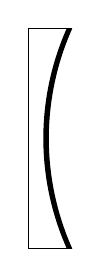
\begin{tikzpicture}[scale=0.7, transform shape]
\def\tmp{65.92}
\fill [black] (0.7,2) arc[start angle=90+\tmp, end angle=270-\tmp,radius=4.9] -- (0.8,-2) -- (0.8,-2) arc[start angle=270-\tmp, end angle=90+\tmp,radius=4.9] -- (0.7,2);
\draw (0.8,-2) -- (0,-2) -- (0,2) -- (0.8,2);
\end{tikzpicture}
\end{center}
\fi
}

% Ü218
\ylDisplay{Lääts} % Ülesande nimi
{Tundmatu autor} % Autor
{lahtine} % Voor
{2007} % Aasta
{G 9} % Ülesande nr.
{7} % Raskustase
{
% Teema: Geomeetriline optika
\ifStatement
Teritamata pliiatsi telg ühtib koondava läätse peateljega. Mitu korda on pliiatsi kujutise pikkus tema enda pikkusest erinev, kui pliiatsi ühe otsa kujutise diameetri ja pliiatsi diameetri suhe on $k_1$ ning teise otsa jaoks on see suhe $k_2$? Pliiatsi mõlemad otsad asuvad läätsest fookuskaugusest suuremal kaugusel.
\fi
}

% Ü219
\ylDisplay{Hajuti} % Ülesande nimi
{Andreas Valdmann} % Autor
{piirkonnavoor} % Voor
{2010} % Aasta
{G 8} % Ülesande nr.
{7} % Raskustase
{
% Teema: Geomeetriline optika
\ifStatement
Mõnedes valgustites kasutatakse valguse hajutamiseks joonisel kujutatud ristlõikega
pleksiklaasist plaati. Valgus langeb selle siledale poolele ja läbib hajuti vaid juhul, kui
langemisnurk on suurem kriitilisest nurgast $\alpha_\mathrm{kr}$. Leidke nurga $\alpha_\mathrm{kr}$ väärtus. Pleksiklaasi
murdumisnäitaja $n=\num{1,5}$. Kõik sakilise poole tahud on \num{45}-kraadise nurga all sileda poole pinna
suhtes.
\begin{center}
	\includegraphics[width=0.475\textwidth]{2010-v2g-08-hajuti.eps}
\end{center}
\fi
}

% Ü220
\ylDisplay{Nõguslääts eestvaates} % Ülesande nimi
{Siim Ainsaar} % Autor
{piirkonnavoor} % Voor
{2011} % Aasta
{G 10} % Ülesande nr.
{7} % Raskustase
{
% Teema: Geomeetriline optika
\ifStatement
Joonisel on kujutatud eestvaates nõguslääts, mille optiline peatelg on joonise tasandiga risti ja lõikub läätsega punktis $O$. Antud on ka üks horisontaalne valguskiir ning selle lõikepunktid eesmise fokaaltasandi ning läätsega (vastavalt punktid $K$ ja $L$). Joonestage antud vaates lisalehel kiire edasine käik ning ta lõikepunkt tagumise fokaaltasandiga. Põhjendage lahendust.
\begin{center}
	\includegraphics[width=0.5\linewidth]{2011-v2g-10-yl}
\end{center}
\fi
}

% Ü221
\ylDisplay{Toru} % Ülesande nimi
{Jaan Kalda} % Autor
{lõppvoor} % Voor
{2012} % Aasta
{G 6} % Ülesande nr.
{7} % Raskustase
{
% Teema: Geomeetriline optika
\ifStatement
Peegeldavate siseseintega toru põhjas on punktvalgusallikas, vt joonist. Toru
sisediameeter on
$d=\SI{12}{mm}$, toru pikkus $l=\SI{60}{mm}$. Vastu toru lahtist otsa on
paigutatud koondav lääts fookuskaugusega $F=\SI{36}{mm}$ ning toru otsast
kaugusele $L=\SI{90}{mm}$ ekraan, millele kinnitatud millimeeterpaberile
on märgitud lõikepunkt optilise peateljega $O$.
Visandage kujutis, mida võib näha ekraanil.

\begin{center}
\includegraphics[width=\textwidth]{2012-v3g-06-toru-valgusallikas-lxxts}
\end{center}
\fi
}

% Ü222
\ylDisplay{Mikroskoop} % Ülesande nimi
{Valter Kiisk} % Autor
{lõppvoor} % Voor
{2013} % Aasta
{G 7} % Ülesande nr.
{7} % Raskustase
{
% Teema: Geomeetriline optika
\ifStatement
Nn digitaalne mikroskoop koosneb piki optilist peatelge nihutatavast
läätsest (objektiivist), mis tekitab vaadeldavast esemest tõelise kujutise
elektroonilise maatrikssensori pinnale. Terav kujutis tekib objektiivi kahe
erineva asendi korral. Vastavate joonsuurenduste suhteks määrati 25. Kummas
asendis ja mitu korda on sensori pinnaühikule langev kiirgusvõimsus suurem?
Võib eeldada, et läätse mõõtmed on palju väiksemad tema kaugusest objektist.
\fi
}

% Ü223
\ylDisplay{Optiline skeem} % Ülesande nimi
{Erkki Tempel} % Autor
{lahtine} % Voor
{2014} % Aasta
{G 7} % Ülesande nr.
{7} % Raskustase
{
% Teema: Geomeetriline optika
\ifStatement
\begin{wrapfigure}{r}{0.5\textwidth}
 \includegraphics[width=0.5\textwidth]{2014-lahg-07-optilineskeemjoonis}
\end{wrapfigure}
Kõrvaloleval joonisel on kujutatud kahe algselt paralleelse kiire käik läbi kahe ühesuguse kumerläätse, mis ei asetse paralleelselt. Läätsede fookused ühtivad ning asuvad punktis F. Konstrueerige skeemile läätsed koos optiliste peatelgedega.
\fi
}

% Ü224
\ylDisplay{Luup} % Ülesande nimi
{Valter Kiisk} % Autor
{lõppvoor} % Voor
{2016} % Aasta
{G 6} % Ülesande nr.
{7} % Raskustase
{
% Teema: Geomeetriline optika
\ifStatement
Kui asetada poolkera-kujuline klaaskeha (lääts) tasapinnalise poolega vastu paberit, on võimalik vähemalt läätse keskosa ümbruses näha paberi pinna suurendatud kujutist. Kui mitmekordne kujutis saadakse, vaadeldes kauguselt, mis on hulga suurem läätse mõõtmetest? Klaasi murdumisnäitaja $n=\num{1.5}$.
\fi
}

% Ü225
\ylDisplay{Gravitatsioonilääts} % Ülesande nimi
{Mihkel Kree} % Autor
{piirkonnavoor} % Voor
{2007} % Aasta
{G 10} % Ülesande nr.
{8} % Raskustase
{
% Teema: Geomeetriline optika
\ifStatement
Üldrelatiivsusteooria ennustab, et mustast august möödumisel kaldub valguskiir gravitatsiooni tõttu kõrvale oma esialgsest liikumissuunast nurga $\varphi = 4GM/c^2r$ võrra, kus $M$ on musta augu mass ning $r$ trajektoori lähima punkti kaugus selleni. Sattugu must auk täpselt vaatleja ja tähe vahele, nii et kaugus vaatlejast musta auguni on $L_1$ ning mustast august täheni $L_2$. Missugune on tähe kujutis vaatleja jaoks (põhjendage oma vastust kiirte käigu visandi abil) ning kui suur on kujutise nurkläbimõõt? Kuna vaatlejani jõudvate kiirte jaoks on $r$ palju väiksem tähe kaugusest, võib kasutada väikeste nurkade lähendust $\sin \alpha \approx \tan \alpha \approx \alpha$.
\fi
}

% Ü226
\ylDisplay{Nurgapeegel} % Ülesande nimi
{Andreas Valdmann} % Autor
{lõppvoor} % Voor
{2016} % Aasta
{G 8} % Ülesande nr.
{8} % Raskustase
{
% Teema: Geomeetriline optika
\ifStatement
\begin{wrapfigure}{r}{0.35\textwidth}
	\vspace{-25pt}
	\begin{center}
		\includegraphics[width=0.35\textwidth]{2016-v3g-08-wink.png}
	\end{center}
	\vspace{-20pt}
\end{wrapfigure}

Jukul oli katsetamiseks kolm ruudukujulist tasapeeglit. Ühte peeglisse vaadates ja paremat silma kinni pigistades nägi ta endast joonisel kujutatud peegelpilti. Järgmisena paigutas Juku kolm peeglit sedasi, et need moodustasid kuubi kolm tahku, millel on üks ühine tipp. Sealjuures jäid peegelpinnad kuubi sisemisele poolele. Joonistage peegelpilt, mida paremat silma kinni pigistav Juku endast otse nurgapeegli nurka vaadates nägi ja põhjendage tulemust konstrueerimise teel.
\fi
}

% Ü227
\ylDisplay{Akvaarium} % Ülesande nimi
{Tundmatu autor} % Autor
{lahtine} % Voor
{2005} % Aasta
{G 10} % Ülesande nr.
{9} % Raskustase
{
% Teema: Geomeetriline optika
\ifStatement
Leidke maksimaalne suurendus $k$, mille tekitab sfääriline akvaarium, kui vaadata väljastpoolt selles ujuvat kala. Suurenduse all mõistame siin kala kujutise ja tegeliku kala suuruste suhet. Vee murdumisnäitaja $n = \num{1,3}$. Väikeste nurkade puhul kehtib ligikaudne võrdus $\sin \alpha \approx \alpha$. 
\fi
}

% Ü228
\ylDisplay{Kuup} % Ülesande nimi
{Jaan Kalda} % Autor
{lõppvoor} % Voor
{2007} % Aasta
{G 8} % Ülesande nr.
{9} % Raskustase
{
% Teema: Geomeetriline optika
\ifStatement
\begin{wrapfigure}[16]{r}{0.5\textwidth}
	\begin{center}
		\vspace{-20pt}
		\includegraphics[width=0.95\linewidth]{2007-v3g-08-yl}
	\end{center}
\end{wrapfigure}
Läbipaistvast klaasist tehtud kuubis on suur kerakujuline õõnsus, mis on täidetud sinist värvi gaasiga. Kuup lebab kollaste seintega toas valgel põrandal. Juuresolev kuubi joonis on tehtud kuubi kohalt pildistatud foto põhjal, millelt on eemaldatud kõik värvid ning jäetud alles selgeltnähtavad kontuurid ja erivärviliste piirkondade eraldusjooned (joonte kujud ja mõõtmed on täpselt sellised nagu fotol). Kuubi mõõtmed lugeda hulga väiksemateks põranda mõõtmetest ning kõrgusest, millelt on tehtud joonise aluseks olnud foto. Millistele värvidele vastavad tähed $A$, $B$, $C$, $D$? Põhjendage vastust. Leidke klaasi murdumisnäitaja.
\fi
}

% Ü229
\ylDisplay{Nõguspeegel} % Ülesande nimi
{Mihkel Kree} % Autor
{lõppvoor} % Voor
{2007} % Aasta
{G 9} % Ülesande nr.
{9} % Raskustase
{
% Teema: Geomeetriline optika
\ifStatement
Optiline süsteem koosneb kumerläätsest ja nõguspeeglist, mille optilised peateljed ühtivad. Kumerpeegli asukohta pole joonisel märgitud. On teada, et objektist $A$ tekib teisele poole läätse kaks kujutist $K_1$ ja $K_2$. Konstrueerige kumerpeegli kõveruskeskpunkt $O$ ja kumerpeeglis objektist $A$ tekkinud näiv kujutis $A'$. Eeldada, et optilises süsteemis on nurgad piisavalt väiksed, et sfäärilisi aberratsioone ei teki.

\begin{center}
	\includegraphics[width=\linewidth]{2007-v3g-09-yl}
\end{center}
\fi
}

% Ü230
\ylDisplay{Kärbes} % Ülesande nimi
{Aigar Vaigu} % Autor
{piirkonnavoor} % Voor
{2008} % Aasta
{G 10} % Ülesande nr.
{9} % Raskustase
{
% Teema: Geomeetriline optika
\ifStatement
Kärbes on merevaigutükis, mille murdumisnäitaja on $n=\num{1,6}$. Tüki üks pinnaosa on sfääriline kõverusraadiusega $r = \SI{3}{mm}$. Kui vaadata kärbse pead läbi selle pinnaosa, siis näib pea asuvat kõveruskeskpunkti läbival sirgel $k = \SI{5}{mm}$ sügavusel merevaigus. Kui sügaval on kärbse pea tegelikult? 

\emph{Märkus}. Kasutada väikeste nurkade lähendust $\tan \alpha \approx \sin \alpha \approx \alpha$, kus $\alpha \gg 1$ on väike nurk mõõdetuna radiaanides.
\fi
}

% Ü231
\ylDisplay{Punktallikad} % Ülesande nimi
{Jaan Kalda} % Autor
{lõppvoor} % Voor
{2010} % Aasta
{G 9} % Ülesande nr.
{9} % Raskustase
{
% Teema: Geomeetriline optika
\ifStatement
Juuresoleval joonisel on neli punkti, millest kaks on valgusallikad ja kaks nende tõelised kujutised, mille on tekitanud õhuke lääts. Leidke konstrueerimise teel läätse tasand ja optiline peatelg. Kui võimalusi on rohkem kui üks, siis leidke need kõik.

\begin{center}
	\includegraphics[width=0.3\linewidth]{2010-v3g-09-punktid}
\end{center}
\fi
}

% Ü232
\ylDisplay{Optiline süsteem} % Ülesande nimi
{Andreas Valdmann} % Autor
{lõppvoor} % Voor
{2011} % Aasta
{G 8} % Ülesande nr.
{9} % Raskustase
{
% Teema: Geomeetriline optika
\ifStatement
Klaasist murdumisnäitajaga $n$ on valmistatud õhuke kaksikkumer lääts, mille mõlema pinna kõverusraadius on $r$ (läätse paksus
$d \gg r$). Läätse üks pind kaetakse peegeldava metallikihiga. Leidke kumerläätsest ja nõguspeeglist tekkinud optilise süsteemi fookuskaugus. 

\emph{Vihje}. Fookuskauguse leidmiseks võib vaadelda optilise peatelje lähedasi kiiri, mis levivad
selle suhtes väikese nurga all. Sel juhul saab rakendada väikeste nurkade valemit $\sin \alpha \approx \tan \alpha \approx \alpha$, kus $\alpha$ on radiaanides. 
\fi
}

% Ü233
\ylDisplay{Ring ja ellips} % Ülesande nimi
{Jaan Kalda} % Autor
{lõppvoor} % Voor
{2015} % Aasta
{G 7} % Ülesande nr.
{9} % Raskustase
{
% Teema: Geomeetriline optika
\ifStatement
Juuresoleval joonisel on kujutatud ring ja sellest koondava läätse poolt tekitatud kujutis. Leidke läätse keskpunkt, optiline peatelg ja fookus.
\begin{center}
\includegraphics[width=0.7\textwidth]{2015-v3g-07-ringjaellips}%
\end{center}
\fi
}

% Ü234
\ylDisplay{Kaamera} % Ülesande nimi
{Ardi Loot} % Autor
{lõppvoor} % Voor
{2017} % Aasta
{G 8} % Ülesande nr.
{9} % Raskustase
{
% Teema: Geomeetriline optika
\ifStatement
Juku pildistab virmalisi iseehitatud kaameraga, mis koosneb ruudukujulisest
valgustundlikust elemendist küljepikkusega $2h=\SI{2.0}{cm}$ ja kumerläätsest
fookuskaugusega $f=\SI{14}{cm}.$ Jukule ei meeldi, et kaamera on
niivõrd suur ja ta tahab, et kaamera oleks maksimaalselt $L_{m}=\SI{7.0}{cm}$
pikk (kaamera pikkus on kaugus valgustundlikust elemendist välimise läätseni).
Selleks paigaldab ta vana kumerläätse asemel uue kumerläätse fookuskaugusega $f_{2}=\SI{3.0}{cm}$
valgustundlikust elemendist kaugusele $L_{m}.$ Kui suure fookuskaugusega
ja kui kaugele kumerläätsest peaks Juku süsteemi
lisama ühe nõgusläätse, et säiliks kaamera esialgne vaatenurk?
\fi
}

% Ü235
\ylDisplay{Sähvatus} % Ülesande nimi
{Mihkel Kree} % Autor
{lõppvoor} % Voor
{2006} % Aasta
{G 9} % Ülesande nr.
{10} % Raskustase
{
% Teema: Geomeetriline optika
\ifStatement
Optiline süsteem koosneb kahest nõguspeeglist ja kumerläätsest (vt joonist), mille optilised peateljed ühtivad. Ringikujulise ristlõikega valgusimpulss siseneb süsteemi optilise peatelje sihis ning valgusvihu telg ühtib sellega. Peeglite kõverusraadiused on $R_1 = \SI{8}{m}$ ja $R_2 = \SI{4}{m}$ ning peeglite vahekaugus $L = \SI{6}{m}$. Peeglite läbimõõdud on $d_1 = \SI{160}{mm}$ ja $d_2 = \SI{96}{mm}$. Kiire läbimõõt on $D = \SI{192}{mm}$. Läätse läbimõõt on suurem valgusvihu omast. Suurema peegli keskel on ava läbimõõduga $d_0 = \SI{1}{mm}$. Joonistage valguse intensiivsuse ajaline kulg kumerläätse fookuses $f$. Eeldage, et süsteemi saabuva impulsi kestvus $\tau \ll L/c$. Valguse kiirus $c = \SI{3e8}{m/s}$.

\begin{center}
	\includegraphics[width=0.95\linewidth]{2006-v3g-09-yl}
\end{center}
\fi
}

% Ü236
\ylDisplay{Klaassilinder} % Ülesande nimi
{Jaan Kalda} % Autor
{lõppvoor} % Voor
{2014} % Aasta
{G 10} % Ülesande nr.
{10} % Raskustase
{
% Teema: Geomeetriline optika
\ifStatement
Klaassilindri välispinnal märgitakse markeriga punkt. Kui seda silindrit vaadata suurelt kauguselt (hulga suuremalt kui silindri raadius) nii, et punkt paistab läbi silindri selle sümmeetriateljel olevat, siis on lisaks näha veel kahte punkti kujutist. Üks kujutis on näha ühel ja teine teisel pool sümmeetriatelge. Kui silindrit keerata ümber oma sümmeetriatelje, siis teatud hetkel sulavad kaks punkti kujutist kokku ning kaovad ära. Kolmas kujutis jääb alles. Kui silindrit edasi keerata, siis hetkel, kui selle pöördenurk algasendi suhtes on \SI{15}{\degree}, kaob ka kolmas kujutis, nõnda et markeriga tehtud punkti polegi enam näha. Kui suur on klaasi murdumisnäitaja?
\fi
}
\newpage\subsection{\protect\StrSubstitute{Kinemaatika}{-}{ }}

% Ü237
\ylDisplay{Autod} % Ülesande nimi
{Oleg Košik} % Autor
{piirkonnavoor} % Voor
{2006} % Aasta
{G 1} % Ülesande nr.
{1} % Raskustase
{
% Teema: Kinemaatika
\ifStatement
Tartu ja Tallinna vahemaa on $s = \SI{180}{km}$. Jalgrattur sõidab Tartust Tallinna poole kiirusega $v_1 = \SI{30}{km/h}$. Sõites luges ta kokku, et $t_0 = \SI{5}{min}$ jooksul tuli talle vastu $n_0 = \SI{20}{autot}$. Mitu Tallinnast Tartusse sõitvat autot on korraga maanteel? Eeldada, et autod sõidavad võrdsete vahemaadega kiirusega $v_2 = \SI{90}{km/h}$ kogu maantee ulatuses.
\fi
}

% Ü238
\ylDisplay{Ummik} % Ülesande nimi
{Jaan Kalda} % Autor
{piirkonnavoor} % Voor
{2007} % Aasta
{G 2} % Ülesande nr.
{1} % Raskustase
{
% Teema: Kinemaatika
\ifStatement
Vaatleme kahe üherajalise tee, $A$ ja $B$, liitumist üherajaliseks teeks $C$. Tipptunni ajal on kõik kolm teed täidetud autodega; kahe naaberauto keskmise vahemaa võib lugeda kõigil kolmel teel ühesuguseks. Tee $A$ pikkus on $L_A = \SI{1}{km}$, tee $B$ pikkus $L_B = \SI{3}{km}$ ning tee $C$ pikkus $L_C = \SI{2}{km}$. Autode keskmine kiirus teel $A$ on $v_A = \SI{3}{km/h}$ ning tee $B$ läbimiseks kulub autol $t_B = \SI{36}{min}$. Kui kaua kulub autol jõudmaks tee $A$ algusest tee $C$ lõpuni?
\begin{center}
	\includegraphics[width=0.9\linewidth]{2007-v2g-02-yl}
\end{center}
\fi
}

% Ü239
\ylDisplay{Auto} % Ülesande nimi
{Tundmatu autor} % Autor
{lahtine} % Voor
{2008} % Aasta
{G 1} % Ülesande nr.
{1} % Raskustase
{
% Teema: Kinemaatika
\ifStatement
Paigalseisust liikuma hakanud autol kulus teatud vahemaa läbimiseks $t = \SI{15}{s}$. Millise ajaga läbis auto viimase viiendiku sellest vahemaast? Auto liikumine lugeda ühtlaselt kiirenevaks.
\fi
}

% Ü240
\ylDisplay{Ratturid} % Ülesande nimi
{Tundmatu autor} % Autor
{lahtine} % Voor
{2009} % Aasta
{G 1} % Ülesande nr.
{1} % Raskustase
{
% Teema: Kinemaatika
\ifStatement
Kolm ratturit sõitsid linnast $A$ linna $B$. Linnast $A$ väljusid nad üheaegselt. Esimese ratturi keskmine kiirus oli $v_1 = \SI{30}{km/h}$, teise ratturi oma $v_2 = \SI{20}{km/h}$. Esimene rattur jõudis sihtpunkti kell 19.00, teine rattur kell 20.00 ning kolmas rattur kell 21.00. Milline oli kolmanda ratturi keskmine kiirus $v_3$?
\fi
}

% Ü241
\ylDisplay{Rong} % Ülesande nimi
{Koit Timpmann} % Autor
{piirkonnavoor} % Voor
{2013} % Aasta
{G 1} % Ülesande nr.
{1} % Raskustase
{
% Teema: Kinemaatika
\ifStatement
Kaubarong läbis kahe jaama vahelise teelõigu keskmise kiirusega \SI{36}{km/h}.
Kogu sõiduajast 2/5 vältel liikus rong ühtlaselt kiirenevalt, siis 2/5 vältel
liikus jääva kiirusega ning viimase 1/5 vältel pidurdas ühtlaselt aeglustuvalt.
Kui suur oli rongi maksimaalne kiirus kahe jaama vahelisel teel?
\fi
}

% Ü242
\ylDisplay{Veok} % Ülesande nimi
{Valter Kiisk} % Autor
{piirkonnavoor} % Voor
{2005} % Aasta
{G 1} % Ülesande nr.
{2} % Raskustase
{
% Teema: Kinemaatika
\ifStatement
Veok sõidab maanteel ühtlase kiirusega $v_1 = \SI{80}{km/h}$. Veokile järgneb $l_1 = \SI{10}{m}$ kaugusel sõiduauto. Veoki pikkus on $L_1 = \SI{12}{m}$, sõiduauto pikkus $L_2 = \SI{4}{m}$. Sõiduauto sooritab möödasõidu ühtlase kiirendusega $a = \SI{2}{m/s^2}$. Möödasõit lõpeb siis, kui sõiduauto on veokist $l_2 = \SI{10}{m}$ kaugusel. Kui pikas minimaalses ulatuses $s$ peaks vastassuunaline rada vaba olema ohutuks möödasõiduks? Ohutuks kauguseks vastutulevast autost loetakse $l_3 = \SI{30}{m}$. Vastutulevad autod sõidavad kiirusega $v_2 = \SI{90}{km/h}$.

\begin{center}
	\includegraphics[width=\linewidth]{2005-v2g-01-yl}
\end{center}
\fi
}

% Ü243
\ylDisplay{Rongiõnnetus} % Ülesande nimi
{Oleg Košik} % Autor
{piirkonnavoor} % Voor
{2011} % Aasta
{G 4} % Ülesande nr.
{2} % Raskustase
{
% Teema: Kinemaatika
\ifStatement
Kehrast Aegviidu poole sõitis kiirusega $v_1=\SI{63}{km/h}$ kaubarong. Aegviidust hakkas sama teed pidi sõitma Kehra poole elektrirong kiirendusega $a_2=\SI{0,15}{m/s^2}$. Kui rongide vahemaa oli $s=\SI{2750}{m}$, märkas kaubarongi vedurijuht vastusõitvat elektrirongi ning vajutas pidurile. Elektrirongi kiirus oli selleks hetkeks $v_2=\SI{18}{km/h}$. Leidke rongide sõidukiirused vahetult kokkupõrke eel. Kaubarongi pidudrdukiirendus on $a_1=-\SI{0,1}{m/s^2}$.
\fi
}

% Ü244
\ylDisplay{Rongivile} % Ülesande nimi
{Mihkel Kree} % Autor
{lahtine} % Voor
{2015} % Aasta
{G 1} % Ülesande nr.
{2} % Raskustase
{
% Teema: Kinemaatika
\ifStatement
Rong läheneb jaamale sirgjooneliselt ning muutumatu kiirusega. Vedurijuht laseb vilet kestusega $t_0=\SI{10}{s}$, peatuses rongi ootav jaamaülem mõõdab vile kestuseks aga $t_1=\SI{9}{s}$. Arvutage rongi liikumise kiirus $v$. Heli kiirus õhus $c=\SI{340}{m/s}$.
\fi
}

% Ü245
\ylDisplay{Kaubarong} % Ülesande nimi
{Erkki Tempel} % Autor
{piirkonnavoor} % Voor
{2015} % Aasta
{G 1} % Ülesande nr.
{2} % Raskustase
{
% Teema: Kinemaatika
\ifStatement
Tavaliselt sõidab kaubarong ühtlase kiirusega $v=\SI{72}{km/h}$, kuid seekord hilines jaama $\Delta t=\SI{5}{min}$. Raudteel olid hooldetööd ning rong pidi mingi aja sõitma kiirusega $v_{h}=\SI{18}{km/h}$. Rongi kiirendus pidurdamisel oli $a_p=\SI{0,2}{m/s^2}$ ning kiirendamisel $a_k=\SI{0,1}{m/s^2}$. Kui pika tee sõitis rong kiirusega \SI{18}{km/h}?
\fi
}

% Ü246
\ylDisplay{Kiirabiauto} % Ülesande nimi
{Sandra Schumann} % Autor
{lahtine} % Voor
{2017} % Aasta
{G 1} % Ülesande nr.
{2} % Raskustase
{
% Teema: Kinemaatika
\ifStatement
Jukust sõitis tänaval mööda kiirabiauto. Juku kuulis, et möödumisel langes kiirabiauto sireeni toon väikese tertsi võrra. Kui kiiresti sõitis kiirabiauto? Heli kiirus õhus Juku juures oli $v_h = \SI{343}{\meter\per\second}$. Eeldada, et Juku kaugus kiirabiauto sirgjoonelisest trajektoorist on tühiselt väike. Doppleri seadus annab seose sageduste ja liikumiskiiruste vahel.
\[ \frac{f_v}{f_a} = \frac{v_h + v_v}{v_h + v_a} \ , \]
kus \(f_v\) on vastuvõtja mõõdetud heli sagedus, \(f_a\) on allika tekitatud heli sagedus, \(v_v\) on heli vastuvõtja kiirus ja \(v_a\) on heliallika liikumise kiirus.

\emph{Vihje}. Väike terts on muusikaline intervall, mis vastab \num{1.5}-toonisele erinevusele heli sageduses. Üks oktav tähistab 2-kordset erinevust heli sageduses ja vastab 6 toonile. Eeldada, et toonid on jaotatud oktavis nõnda, et kui kolme helisageduse $f_1, f_2, f_3$ jaoks kehtib $\frac{f_2}{f_1} = \frac{f_3}{f_2}$ ja $f_1$ ning $f_2$ vahel on üks toon, siis on ka $f_2$ ja $f_3$ vahel üks toon.
\fi
}

% Ü247
\ylDisplay{Pidurdus} % Ülesande nimi
{Mihkel Rähn} % Autor
{piirkonnavoor} % Voor
{2017} % Aasta
{G 2} % Ülesande nr.
{2} % Raskustase
{
% Teema: Kinemaatika
\ifStatement
Kaks autot sõidavad teineteise järel kiirustega $v=\SI{50}{km/h}$. Esimene auto pidurdab maksimaalselt, mida nähes tagumise auto juht samuti pidurdab maksimaalselt. Esimese auto pidurid rakenduvad samal hetkel, kui süttivad pidurituled. Tagumise auto juhil kulub eesmise auto piduritulede süttimisest kuni oma auto pidurite rakendumiseni $t=\SI{1,5}{s}$. Teekatte hõõrdetegur $\mu=1$ ning raskuskiirendus $g=\SI{9,8}{m/s^2}$.\\
\osa Kui suur peaks olema autodevaheline vahemaa sõidu ajal, et pidurdamisel ei toimuks tagant otsasõitu?\\
\osa Kui autodevaheline vahemaa enne pidurdamist on $l=\SI{5}{m}$, siis kui suur on autode kiirus üksteise suhtes kokkupõrke hetkel?
\fi
}

% Ü248
\ylDisplay{Sonar} % Ülesande nimi
{Oleg Košik} % Autor
{piirkonnavoor} % Voor
{2006} % Aasta
{G 3} % Ülesande nr.
{3} % Raskustase
{
% Teema: Kinemaatika
\ifStatement
Vaatame järgmist meetodit laeva kiiruse määramiseks. Saadame rannikult sellest eemalduvale laevale ultraheli signaali sagedusega $f_1$. Laevalt peegeldub signaal tagasi rannikule, kus vastuvõtja fikseerib signaali sagedusega $f_2$. Teades, et heli kiirus õhus on $v_h$, määrake laeva kiirus $v$.
\fi
}

% Ü249
\ylDisplay{Autod} % Ülesande nimi
{Jaan Kalda} % Autor
{piirkonnavoor} % Voor
{2008} % Aasta
{G 2} % Ülesande nr.
{3} % Raskustase
{
% Teema: Kinemaatika
\ifStatement
Juuresolev joonis on tehtud kõrgelt otse alla pildistatud foto põhjal, millel on jäädvustatud kaks autot (tähistatud punktidega $A$ ja $B$), mis lähenevad ristmikule jäävate kiirustega $v_A = \SI{40}{km/h}$ ja $v_B = \SI{60}{km/h}$. Kasutades joonist ja sellel antud mõõtkava, leidke autode edasisel liikumisel nende vaheline minimaalne kaugus.

\begin{center}
	\includegraphics[width=0.9\linewidth]{2008-v2g-02-yl}
\end{center}
\fi
}

% Ü250
\ylDisplay{GPS} % Ülesande nimi
{Jaan Kalda} % Autor
{lõppvoor} % Voor
{2009} % Aasta
{G 5} % Ülesande nr.
{4} % Raskustase
{
% Teema: Kinemaatika
\ifStatement
Tervisesportlane kasutab GPS seadet oma jooksutreeningu tulemuste salvestamiseks.
Tema GPS seade määrab iga 15 sekundi järel jooksja täpse asukoha, mille põhjal arvutab ja salvestab GPS seade viimase 15 sekundi keskmise kiiruse.
GPS esitab saadud tulemused graafikul punktidena, mis on ühendatud sirglõikude abil.
Jooksja märkas, et ketsipael oli lahti läinud.
Ta peatus, sidus selle kinni ning tänu väikesele puhkusele jätkas jooksu juba natuke suurema
kiirusega, vt juuresolevat GPS-i esitatud graafikut. Kui kaua kestis peatus? Pidurdumiseks ning puhkusjärgselt kiirendamiseks kulunud
aeg lugeda tühiseks; jooksu kiirus oli konstantne nii enne peatust kui ka pärast seda.

\begin{center}
\includegraphics{2009-v3g-05-gps.eps}
\end{center}
\fi
}

% Ü251
\ylDisplay{Jalgrattur} % Ülesande nimi
{Jaan Kalda} % Autor
{lõppvoor} % Voor
{2013} % Aasta
{G 3} % Ülesande nr.
{4} % Raskustase
{
% Teema: Kinemaatika
\ifStatement
Poiss mõõdab jalgrattaga sõites tuule kiirust enda suhtes: kui ta sõidab piki teed ühes
suunas kiirusega \SI{10}{km/h}, saab ta tulemuseks \SI{20}{km/h}, ning kui ta sõidab
vastassuunas kiirusega \SI{20}{km/h}, siis saab ta tulemuseks samuti
\SI{20}{km/h}. Kui kiiresti maa suhtes puhub tuul?
\fi
}

% Ü252
\ylDisplay{Viiul} % Ülesande nimi
{Jaan Toots} % Autor
{lõppvoor} % Voor
{2014} % Aasta
{G 2} % Ülesande nr.
{4} % Raskustase
{
% Teema: Kinemaatika
\ifStatement
Viiulikeelt pikkusega $L$ kaugusel $\frac{3}{7}L$ ühest otsast alla vajutades ning lühemal osal poognaga tõmmates kõlab mingi põhisagedusega heli. Samal kaugusel $\frac{3}{7}L$ keelt ainult puudutades (alla vajutamata), on kõlav heli erinev. Milline on nende kahe põhisageduse suhe?
\fi
}

% Ü253
\ylDisplay{Pöördlava} % Ülesande nimi
{Taavi Pungas} % Autor
{piirkonnavoor} % Voor
{2012} % Aasta
{G 4} % Ülesande nr.
{5} % Raskustase
{
% Teema: Kinemaatika
\ifStatement
Sageli on teatrilava põranda osaks pöörlev ketas. Näitleja soovib sellise ketta
kõrval olevast punktist $A$ ajaga $t$ jõuda võimalikult kaugele mõnda teise ketta
kõrval olevasse punkti. Kus asub selline kaugeim sihtpunkt $B$? Väljendage vastus nurgana
$\alpha = \angle \mathit{AOB}$, kus $O$ on ketta keskpunkt. Näitleja kõnnib
kiirusega $v$, ketta pöörlemisperiood on $T$ ja raadius $r$. Võite eeldada, et $\alpha < 180\degree$.
\fi
}

% Ü254
\ylDisplay{Pallivise} % Ülesande nimi
{Eero Vaher} % Autor
{lõppvoor} % Voor
{2015} % Aasta
{G 5} % Ülesande nr.
{5} % Raskustase
{
% Teema: Kinemaatika
\ifStatement
Juku elab silindrikujulises kosmosejaamas, mille pöörlemine tekitab kunstliku raskusjõu. Jaama raadius on $R$, selle pöörlemise nurkkiirus $\omega$. Juku viskab palli otse üles algkiirusega $v=\frac{\sqrt{3}}{3}\omega R$. Kui kaugele Jukust mööda jaama pinda pall maandub?
\fi
}

% Ü255
\ylDisplay{Tsunami} % Ülesande nimi
{Jaan Kalda} % Autor
{lõppvoor} % Voor
{2005} % Aasta
{G 6} % Ülesande nr.
{6} % Raskustase
{
% Teema: Kinemaatika
\ifStatement
\begin{wrapfigure}[10]{r}{0.45\textwidth}
	\begin{center}
		\vspace{-20pt}
		\includegraphics[width=\linewidth]{2005-v3g-06-yl}
	\end{center}
\end{wrapfigure}

Joonisel on ülaltvaates toodud ookeanipõhja sügavus kodeeritud halltoonidega: tumedam hall vastab sügavamale, heledam hall madalamale veele. Ookeanipõhjas on astang, kus $h_1 = \SI{5000}{m}$ sügavune vesi läheb $h_2 = \SI{3200}{m}$ sügavuseks; ranna lähedal toimub madaldumine väga kiiresti. Rannale läheneb tsunami nii, nagu näidatud joonisel. Tsunami liikumiskiirus $v = \sqrt{gh}$, kus $g = \SI{9,8}{m/s^2}$ ja $h$ tähistab vee sügavust. Millisesse ranna punkti jõuab kõige kõrgem laine? Põhjendage vastust.
\fi
}

% Ü256
\ylDisplay{Hävituslennuk} % Ülesande nimi
{Tundmatu autor} % Autor
{lahtine} % Voor
{2011} % Aasta
{G 7} % Ülesande nr.
{6} % Raskustase
{
% Teema: Kinemaatika
\ifStatement
Ühel ilusal augustipäeval käis Mati paraadil vaatamas NATO hävituslennukeid, mis
tegid üle rahva peade demonstratsioonlende. Diktor ütles valjuhääldist, et lennuk
lendab horisontaalselt üle rahva kiirusega $v=\SI{1350}{km/h}$. Matit huvitas aga, kui
kõrgel lennuk lendab. Vajalike mõõtetulemuste saamiseks seisis ta nii, et tema
ja läheneva lennukiga ühele joonele jäi täpselt üks 9 meetri pikkune elektripost
ning Mati ise asus teise posti juures; postide vahekaugus oli \SI{50}{m}. Mati käivitas oma
mobiiltelefoni stopperi just siis, kui lennuk ilmus posti otsa tagant nähtavale ning 
peatas hetkel, kui käis kõva pauk ja hakkas kostuma lennuki müra. Ta sai
stopperi näiduks \SI{32,04}{s}. Kodus
mõõtis ta üle ka enda silma kõrguse maapinnast: $l=\SI{1,68}{m}$.
Kui kõrgel lendas lennuk? Heli kiirus õhus on umbes
$u=\SI{330}{m/s}$.\\ 
\textit{Vihje.} Kui lennuk lendab
ülehelikiirusel, siis levib tema taga
koonusekujuline lööklaine front, kusjuures koonuse tipus on lennuk ja selle
koonuse telglõike
tipunurk on $\alpha=2\arcsin\left(\frac{u}{v}\right)$.
\fi
}

% Ü257
\ylDisplay{Rehvid} % Ülesande nimi
{Siim Ainsaar} % Autor
{lõppvoor} % Voor
{2012} % Aasta
{G 5} % Ülesande nr.
{6} % Raskustase
{
% Teema: Kinemaatika
\ifStatement
Et autorehvid kuluksid vähimal määral, tasub auto ehitada nii, et kurvis
pöörduksid esirattad eri nurga võrra. Leidke selles mõttes parim parema
esiratta pöördenurk $\beta$ paremkurvis, kus
vasaku esiratta oma on $\alpha$. Rataste vahekaugus on pikkupidi $a$ ja laiupidi
$b$ (vt joonist).
\begin{center}
\includegraphics[width=0.3\linewidth]{2012-v3g-05-r_yl_joonis}%
\end{center}
\fi
}

% Ü258
\ylDisplay{Kammid} % Ülesande nimi
{Jaan Kalda} % Autor
{lõppvoor} % Voor
{2014} % Aasta
{G 5} % Ülesande nr.
{6} % Raskustase
{
% Teema: Kinemaatika
\ifStatement
\begin{wrapfigure}{r}{0.6\textwidth}%
\includegraphics[width=1\linewidth]{2014-v3g-05-kammid}
\end{wrapfigure}

Kaks kammi on asetatud üksteise taha nii, nagu näidatud joonisel. Halli kammi liigutatakse kiirusega $v=\SI 1{cm/s}$ ning musta kammi hoitakse paigal. Millise kiirusega ja millises suunas liiguvad tumedad laigud?
\fi
}

% Ü259
\ylDisplay{Fotograaf} % Ülesande nimi
{Jaan Kalda} % Autor
{lõppvoor} % Voor
{2011} % Aasta
{G 6} % Ülesande nr.
{7} % Raskustase
{
% Teema: Kinemaatika
\ifStatement
Fotograaf pildistas kõrgest joast langevat veevoolu; päikesevalguses sätendavad veepiisad venisid piltidel vertikaalseteks triipudeks.
Kui fotoaparaat oli pildistamisel normaalasendis, siis olid kõik triibud pikkusega $l_1 = \num{120}$ pikslit; kui fotoaparaat oli pildistamisel \enquote{jalad ülespidi} (st seda
pöörati ümber optilise telje \num{180} kraadi), siis oli triipude pikkuseks $l_2 = \num{200}$
pikslit. Kui pikad olid triibud siis, kui fotoaparaati hoiti pildistamisel \enquote{portree
asendis} (st seda pöörati ümber optilise telje \num{90} kraadi)? Eeldada, et säriaeg
ja optilise telje suund oli kõigil juhtudel üks ja sama. Kui toodud andmete
põhjal pole vastus üheselt leitav, siis andke kõik võimalikud vastused.

\emph{Vihje}. 
Fotoaparaadi põhikomponendid on objektiiv (lääts) ja katik, millest
esimene tekitab digitaalsensori (või filmi) tasandile pildistatavate esemete kujutise. \enquote{Puhkeasendis} ei lange see kujutis siiski sensorile, sest katik varjab
läbi objektiivi tulnud valguse ära. Päästikule vajutamisel avaneb katik lühikeseks ajavahemikuks (säriajaks): objektide kujutis langeb nüüd tõesti sensorile
ning sensori iga piksel mõõdab ära kogu selle aja vältel langeva valgusenergia.
Harilikult kujutab katik endast kahte \enquote{kardinat}, mis paiknevad vahetult sensori ees ja katavad selle. Alguses varjab sensorit esimene kardin, mille ülemine
serv liigub päästikule vajutamisel konstantse kiirusega $v$ ülevalt alla, avades
sensori. Säriaja lõpetab teine kardin, mille alumine serv liigub samuti ülevalt
alla, samasuguse kiirusega $v$ nagu esimenegi. Kui säriaeg on hästi lühike, siis
ei jõua sensor täielikult avaneda: mõlemad kardinad liiguvad koos ülevalt alla
ning sensor on avatud objektiivist tulevale valgusele vaid kardinate vahelise
kitsa horisontaalse riba ulatuses (kusjuures see valgusele avatud riba liigub
kiirusega $v$ ülevalt alla).
\fi
}

% Ü260
\ylDisplay{Laev} % Ülesande nimi
{Tundmatu autor} % Autor
{lõppvoor} % Voor
{2007} % Aasta
{G 5} % Ülesande nr.
{8} % Raskustase
{
% Teema: Kinemaatika
\ifStatement
Maailmas leidub jõgesid, kus vesi tõusude tõttu liigub kord ühes, kord teises suunas. Vaatleme laevaliiklust ühel sellisel jõel. Joonisel on antud vee liikumiskiiruse sõltuvus kellaajast. Positiivseks loetakse vee kiirus siis, kui see on suunatud punktist $A$ punkti $B$ poole. Leida optimaalne (lühimate sõiduaegadega) tunniplaan kaubalaeva regulaarseks liikumiseks üks kord päevas punktist $A$ punkti $B$ ja tagasi. Kaugus nende punktide vahel piki jõge on $L = \SI{20}{km}$, laeva kiirus seisvas vees $v_0 = \SI{4}{km/h}$.

\begin{center}
	\includegraphics[width=0.7\linewidth]{2007-v3g-05-yl}
\end{center}
\fi
}

% Ü261
\ylDisplay{Müra} % Ülesande nimi
{Siim Ainsaar} % Autor
{lahtine} % Voor
{2009} % Aasta
{G 10} % Ülesande nr.
{8} % Raskustase
{
% Teema: Kinemaatika
\ifStatement
Matkaja on laagriplatsil õnnelik, et elektrijaama müra temani tuuletu ilmaga nii vaikselt kostab. Veidi hiljem, tuulega, on müra veel tasasem. Puhub põhjatuul kiirusega $\beta c$, kus $c$ on heli kiirus paigalseisvas õhus; jaam jääb matkajast edelasse
(st tuule ja jaama suundade vaheline nurk on $\alpha = \SI{135}{\degree}$).\\
\osa Kas helisagedus on sama mis tuuleta?\\
\osa Kui tuuleta on tajutav helivõimsus $P$ ja tuulega $xP$, siis kui suur on $x$?\\
Võite lugeda, et elektrijaam on punktikujuline. 

\emph{Soovitus}. Uurige helifrondi levimist
\fi
}

% Ü262
\ylDisplay{Kaater} % Ülesande nimi
{Jaan Kalda} % Autor
{lõppvoor} % Voor
{2009} % Aasta
{G 8} % Ülesande nr.
{8} % Raskustase
{
% Teema: Kinemaatika
\ifStatement
Mootorpaat sõidab jõe ühelt kaldalt punktist A teisele kaldale punkti B. Paadi kiirus on $u=\SI{7}{m/s}$.\\
\osa Joonisel on näidatud paadi tekitatud veelained. Milline on jõe voolukiirus?\\
\osa On teada, et kui vee sügavus on $h$, siis lained levivad kiirusega $w=\sqrt{gh}$, kus $g$ on vabalangemise kiirendus.
Kui sügav on jõgi?

\begin{center}
\includegraphics[width=0.55\linewidth]{2009-v3g-08-paat.eps}
\end{center}
\fi
}

% Ü263
\ylDisplay{Päikese pöörlemine} % Ülesande nimi
{Mihkel Kree} % Autor
{lahtine} % Voor
{2014} % Aasta
{G 10} % Ülesande nr.
{8} % Raskustase
{
% Teema: Kinemaatika
\ifStatement
Maa pöörleb ümber oma telje perioodiga $T_\text{m}\approx\SI{24}{h}$. Ka Päike pöörleb ümber oma telje. Selles võib veenduda näiteks päikeseplekkide liikumist jälgides, aga selles ülesandes kasutame hoopis infot Päikese ketta serval paiknevatest ekvaatori punktidest A ja B kiiratud spektrite kohta. Osutub, et kui mõõdetakse naatriumi kollase neeldumisjoone lainepikkusi, siis punktidest A ja B kiiratud spektritest saadakse selle lainepikkuse jaoks veidi erinevad väärtused. Mõõdetud lainepikkused erinevad teineteisest $\Delta \lambda = \SI{7.8}{pm}=\SI{7.8e-12}{m}$ võrra. Naatriumi kollase neeldumisjoone laboratoorne lainepikkus on $\lambda_0=\SI{590}{nm}$, valguse kiirus $c=\SI{3.0e8}{m/s}$, Päikese raadius $r=\SI{700000}{km}$. Leidke Päikese ekvatoriaalpiirkonna pöörlemisperiood $T_\text{p}$.
\fi
}

% Ü264
\ylDisplay{Traatrõngad} % Ülesande nimi
{Jaan Kalda} % Autor
{lõppvoor} % Voor
{2014} % Aasta
{G 9} % Ülesande nr.
{8} % Raskustase
{
% Teema: Kinemaatika
\ifStatement
Kaks ühesugust traatrõngast raadiusega $R$ on üksteise vahetus läheduses, rõngaste tasandid on paralleelsed ning rõngad puudutavad üksteist punktides $A$ ja $B$. Kaarele $AB$ vastav kesknurk on vaadeldaval ajahetkel $\alpha$. Alumine rõngas on paigal, ülemine pöörleb nurkkiirusega $\omega$ ümber punkti $A$ läbiva ning rõngaste tasanditega risti oleva telje. Leidke rõngaste puutepunkti $B$ kiirus antud ajahetkel.
\fi
}

% Ü265
\ylDisplay{Kodarad} % Ülesande nimi
{Tundmatu autor} % Autor
{lahtine} % Voor
{2011} % Aasta
{G 10} % Ülesande nr.
{9} % Raskustase
{
% Teema: Kinemaatika
\ifStatement
\begin{wrapfigure}[8]{r}{40mm}
	\vspace{-10pt}
	\includegraphics[width=40mm]{2011-lahg-10-kodar.pdf}
\end{wrapfigure}
Radiaalsete kodaratega rattast, mis veereb horisontaalsel pinnal, tehakse pilt.
Fotokaamera säriaeg on mõõduka pikkusega: paigalseisvad objektid on pildil teravad, 
liikuvad esemed aga hägused. Muuhulgas on ratta kodarad valdavalt hägusad, 
kuid osa kodarate teatud punktid on ometigi teravad. Võite eeldada, et kogu pilt on 
salvestatud samaaegselt. 
\\
\osa Kopeerige juuresolev skeem lahenduslehele ning näidake konstruktsiooni teel, 
milline kodara $OP$ punkt (või punktid) kujutub fotol teravalt; põhjendage vastust.\\
\osa Konstrueerige kõver, millel asuvad ülejäänud kodarate teravalt kujutuvad punktid.
\fi
}

% Ü266
\ylDisplay{Anemomeeter} % Ülesande nimi
{Jaan Kalda} % Autor
{lahtine} % Voor
{2016} % Aasta
{G 9} % Ülesande nr.
{9} % Raskustase
{
% Teema: Kinemaatika
\ifStatement
Ultraheli anemomeeter mõõdab tuule kiirust sel teel, et määrab aja, mis kulub helisignaalil allikast senosoriteni jõudmiseks.
Olgu heliallikas koordinaatide alguspunktis $O=(0;0)$ ning kolm sensorit punktides koordinaatidega $A=(0;a)$, $B=(a;0)$ ja $C=(-a;0)$, 
kus $a=\SI{211.1}{mm}$ (loeme lihtsustavalt, et nii heliallika kui ka sensorite mõõtmed on tühised). 
Anemomeetrit hoitakse nii, et kõik sensorid paiknevad ühes ja samas horisontaaltasandis ning helisignaali 
sensoriteni jõudmise aegadeks mõõdetakse vastavalt $t_A=\SI{627,0}{\micro s}$, $t_B=\SI{625,2}{\micro s}$ ja $t_C=\SI{603,4}{\micro s}$. 
Milline on tuule kiirus? Arvutustes võite kasutada mõistlikke lihtsustavaid lähendusi.
\fi
}

% Ü267
\ylDisplay{Kaater} % Ülesande nimi
{Jaan Kalda} % Autor
{lõppvoor} % Voor
{2016} % Aasta
{G 9} % Ülesande nr.
{9} % Raskustase
{
% Teema: Kinemaatika
\ifStatement
Kaater sõitis $l=\SI 4{km}$ kaugusel otse lõuna suunas asuvale saarele. 
Alguses võeti suund esimesele meremärgile, seejärel pöörati teise suunas ning lõpuks võeti kurss otse saare peale; seega koosnes trajektoor kolmest sirglõigust. Kaatrilt mõõdeti tuule kiirust ja suunda: esimest lõiku sõideti $t_1=\SI{3}{min}$ ja tuule kiiruseks mõõdeti $v_1=\SI{15}{m/s}$ ning tajutav suund oli otse idast, teist lõiku sõideti $t_2=\SI{1,5}{min}$ ja tuule kiiruseks mõõdeti $v_2=\SI{10}{m/s}$ ning tajutav suund oli otse kagust (lõuna-ida vahelt), kolmandat lõiku sõideti $t_3=\SI{1,5}{min}$ ja tuule kiiruseks mõõdeti $v_3=\SI{5}{m/s}$ ning tajutav suund oli otse edelast (lõuna-lääne vahelt). Mis oli tegelik tuule kiirus?

\emph{Märkus.} Eri lõikudel võis paadi kiirus olla erinev, kuid iga lõigu kestel hoiti konstantne; pööramiseks ja kiirendamiseks kulunud aeg oli tühine; tuule tegelik suund ja kiirus ei muutunud. 
\fi
}

% Ü268
\ylDisplay{Propeller} % Ülesande nimi
{Andreas Valdmann} % Autor
{lõppvoor} % Voor
{2010} % Aasta
{G 10} % Ülesande nr.
{10} % Raskustase
{
% Teema: Kinemaatika
\ifStatement
See pilt pöörlevast lennukipropellerist on tehtud telefoni kaameraga, mis salvestab korraga ühe vertikaalse veeru pikselid. Pilt tekib vasakult paremale veergude kaupa skaneerides.\\
\osa Mis suunas pöörleb propeller fotograafi poolt vaadatuna (päripäeva või vastupäeva)?\\
\osa Mitu laba on propelleril?\\
\osa Mitu pööret teeb propeller ühes minutis, kui kogu pildi tegemiseks kulunud aeg on 1/8 sekundit?\\

\begin{center}
	\includegraphics[width=90mm]{2010-v3g-10-Propeller.jpg}
\end{center}
\fi
}
\newpage\subsection{\protect\StrSubstitute{Laineoptika}{-}{ }}

% Ü269
\ylDisplay{Kile} % Ülesande nimi
{Jaan Kalda} % Autor
{lahtine} % Voor
{2008} % Aasta
{G 8} % Ülesande nr.
{7} % Raskustase
{
% Teema: Laineoptika
\ifStatement
Selleks, et vähendada peegeldusi optilistelt klaasidelt, kaetakse nende pinnad õhukese läbipaistva kilega. Leida, millise paksusega peaks olema selline kile, kui klaasi murdumisnäitaja on $n_0 = \num{1,5}$ ja kile oma $n_1 = \num{1,3}$. Eeldada, et kile on optimeeritud risti langeva rohelise valguse jaoks lainepikkusega $\lambda = \SI{530}{nm}$.
\fi
}

% Ü270
\ylDisplay{Kunstinäitus} % Ülesande nimi
{Jaan Kalda} % Autor
{lõppvoor} % Voor
{2009} % Aasta
{G 10} % Ülesande nr.
{9} % Raskustase
{
% Teema: Laineoptika
\ifStatement
Kunstinäituse saal kujutab endast valgete seintega suurt tuba, mida valgustatakse monokromaatilise rohelise valgusega (lainepikkus $\lambda=\SI{550}{nm}$).
Sellel toal on siledast klaasist põrand; klaasi
alumine pind on värvitud mustaks, ülemine pind on aga kaetud õhukese läbipaistva värvitu kilega.
Keset tuba seisev näitusekülastaja
näeb enda ümber põrandal heledaid ja tumedaid ringikujulisi vööte, kusjuures ta ise asub nende ringide keskpunktis --- sõltumata sellest, kus kohas ta parajasti seisab. Näitusekülastaja uurib asja lähemalt: kükitab ja vaatab kaugele, seejärel püüab vaadata otse alla. Maksimaalselt õnnestub tal loendada $N=\num{20}$ heledat vööti. Kui paks on klaasi kattev kile?
Klaasi murdumisnäitaja $n_0=\num{1.6}$, seda katva kile oma $n_1=\num{1.4}$.
\fi
}
\newpage\subsection{\protect\StrSubstitute{Magnetism}{-}{ }}

% Ü271
\ylDisplay{Magnetpeegel} % Ülesande nimi
{Kristian Kuppart} % Autor
{lahtine} % Voor
{2013} % Aasta
{G 2} % Ülesande nr.
{3} % Raskustase
{
% Teema: Magnetism
\ifStatement
Positiivse laenguga $q$ ja kiirusega $v$ osake liigub ristkülikukujulise riba poole nii, et tema kiirusvektor
moodustab riba normaaliga nurga $\alpha$. Riba paksus on $d$ ja seal paikneb
homogeenne $z$-telje suunaline
magnetväli induktsiooniga $B$ (paberi tasandist meie poole suunatud). Millise maksimaalse
langemisnurga $\alpha_{\mathrm{max}}$ korral
osake veel läbib magnetvälja? On teada, et ribaga risti sellesse sisenev osake
läbiks riba.

\begin{center}
\includegraphics[width=\linewidth]{2013-lahg-02-magnetpeegeljoonis_ipe}
\end{center}
\fi
}

% Ü272
\ylDisplay{Solenoid} % Ülesande nimi
{Andres Laan} % Autor
{lõppvoor} % Voor
{2011} % Aasta
{G 5} % Ülesande nr.
{4} % Raskustase
{
% Teema: Magnetism
\ifStatement
Õhksüdamikuga solenoidis (pikas silindrilises poolis) on vool
$I$. Solenoidi sisemuses liigub elektron, mille trajektoor kujutab endast sellist
kruvijoont, mille keerdude arv on võrdne solenoidi keerdude arvuga. Leidke
selle elektroni kiiruse teljesihiline komponent. Võib eeldada, et elektroni kiiruse teljega risti olev komponent on piisavalt väike, et kokkupõrkeid solenoidi
seinaga ei toimu. Elektroni mass on $m$ ja laeng $e$.

\emph{Vihje}. Solenoidi sees on
homogeenne magnetväli induktsiooniga $B = \mu_0nI$, kus $n$ on solenoidi traadi
keerdude arv pikkusühiku kohta, $I$ selles olev vool ja $\mu_0$ vaakumi magnetiline
läbitavus.
\fi
}

% Ü273
\ylDisplay{Generaator} % Ülesande nimi
{Andreas Valdmann} % Autor
{lahtine} % Voor
{2013} % Aasta
{G 5} % Ülesande nr.
{4} % Raskustase
{
% Teema: Magnetism
\ifStatement
Teatud tüüpi elektrigeneraatoris pöörleb väljundiga ühendatud juhtmekontuur
püsimagnetitega tekitatud magnetväljas, muutes mehaanilise töö elektrienergiaks.
Sellise generaatori külge oli tarbijana ühendatud elektrilamp. Esialgu aeti
generaatorit ringi nurkkiirusega $\omega_0$, mille tulemusel eraldus lambis
võimsus $P_0$. Mingil hetkel suurendati generaatori pöörlemissagedust 2 korda.\\
\osa Kui suur oli lambis eralduv võimsus pärast pöörlemissageduse suurendamist?\\
\osa Kui suur oli generaatori ringiajamiseks tarvilik jõumoment enne ja
pärast pöörlemissageduse suurendamist?

Võib eeldada, et generaator töötas kadudeta ehk kogu tema ringiajamisel tehtav
töö kandus üle tarbijale. Ühtlase sagedusega pöörlemisel on generaatorit
ringiajav jõumoment konstantne. Samuti võib eeldada, et lambi takistus ei sõltu
teda läbiva voolu tugevusest.
\fi
}

% Ü274
\ylDisplay{Tiirlev kuulike} % Ülesande nimi
{Eero Vaher} % Autor
{lahtine} % Voor
{2013} % Aasta
{G 6} % Ülesande nr.
{5} % Raskustase
{
% Teema: Magnetism
\ifStatement
Olgu meil positiivselt laetud kuulike massiga $m$. On teada, et kui kuulike
liiguks kiirusega $v$ sellega ristuvas magnetväljas induktsiooniga $B$,
siis oleks selle trajektooriks ringjoon raadiusega~$r$. Kui suure laenguga $q$ peab olema teine sama massiga kuulike, et esimene
kuulike liiguks teise kuulikese elektriväljas sama kiirusega samal trajektooril? Eeldage, et
kahe kuulikese süsteemile ei mõju väliseid jõude. Kõiki liikumisi vaadeldakse
laboratoorses taustsüsteemis.
\pagebreak
\fi
}

% Ü275
\ylDisplay{Langev takisti} % Ülesande nimi
{Andres Laan} % Autor
{piirkonnavoor} % Voor
{2011} % Aasta
{G 8} % Ülesande nr.
{6} % Raskustase
{
% Teema: Magnetism
\ifStatement
\begin{wrapfigure}{r}{0.2\textwidth}
	\vspace{-20pt}	
	\begin{center}
		\includegraphics[width=0.9\linewidth]{2011-v2g-08-yl}
	\end{center}
	\vspace{-20pt}
\end{wrapfigure}

Joonisel kujutatud Maa gravitatsiooniväljas vertikaalselt paiknevale juhtivale traadile kinnitati takisti nõndaviisi, et see võib piki traati vabalt libiseda. Teades, et magnetinduktsioon oli $B$ ja traadi harude vaheline kaugus $d$, leidke, millise lõppkiirusega hakkab takisti langema. Takisti mass on $m$ ja takistus $R$.
\fi
}

% Ü276
\ylDisplay{Tsüklotron} % Ülesande nimi
{Kristian Kuppart} % Autor
{piirkonnavoor} % Voor
{2018} % Aasta
{G 10} % Ülesande nr.
{6} % Raskustase
{
% Teema: Magnetism
\ifStatement
\begin{wrapfigure}{r}{0.35\linewidth}
	\begin{center}
		\includegraphics[width=\linewidth]{2018-v2g-10-tsyklotron}
	\end{center}
\end{wrapfigure}

Vaatleme tsüklotroni -- teatud tüüpi osakestekiirendi toimimist. Tsüklotron koosneb silindrikujulisest piirkonnast raadiusega $R$, kus on homogeenne magnetväli tugevusega $B$, ning õhukesest ribakujulisest piirkonnast laiusega $d$, kus on homogeenne ribaga risti olev elektriväli tugevusega $E$. Elektrivälja suunda muudetakse perioodiliselt vastassuunaliseks nii, et osakeste igal riba läbimisel on elektrivälja suund osakeste kiirusvektoriga samasuunaline. Samuti on tsüklotroni ühes ääres osakeste tsüklotronist väljumiseks kitsas kanal. Alustagu osakesed liikumist tsüklotroni keskelt tühiselt väikse algkiirusega. Mitu täisringi $n$ teevad osakesed tsüklotronis enne väljumist? Osakeste laeng on $q$ ja mass $m$. Eeldada, et $n\gg 1.$
\fi
}

% Ü277
\ylDisplay{Laengud} % Ülesande nimi
{Jaan Kalda} % Autor
{lahtine} % Voor
{2011} % Aasta
{G 6} % Ülesande nr.
{7} % Raskustase
{
% Teema: Magnetism
\ifStatement
Kaks osakest laenguga $q$ stardivad koordinaatide alguspunktist kiirusega $v$:
üks $x$-telje sihis, teine $y$-telje sihis.
Liikumine toimub homogeenses $z$-telje sihilises magnetväljas induktsiooniga
$B$; osakeste omavahelise
elektrostaatilise vastasmõjuga ärge arvestage. Milline on osakeste vahelise
kauguse maksimaalväärtus $l_{\max}$ edasise liikumise käigus?
\fi
}

% Ü278
\ylDisplay{Mass-spektromeeter} % Ülesande nimi
{Kristian Kuppart} % Autor
{piirkonnavoor} % Voor
{2013} % Aasta
{G 10} % Ülesande nr.
{7} % Raskustase
{
% Teema: Magnetism
\ifStatement
\begin{wrapfigure}[4]{r}{3cm}%
\includegraphics[width=\linewidth]{2013-v2g-10-massspektromeeter_ipe}%
\end{wrapfigure}
Laboris oli uurimiseks hulk mingit atomaarset ainet, mille molaarmassiks mõõdeti
$\mu_{1}$. Ühekordselt ioniseeritud ainet (iga aatom oli kaotanud ühe
elektroni) kiirendati elektriväljas potentsiaalide vahega $U$ ja suunati magnetvälja
induktsiooniga $B$ (vaadake joonist). Magnetinduktsioon oli joonise tasandiga
risti, 
ioonide algkiirus oli $y$-telje suunaline,
magnetväli asus piirkonnas $y>0$ ning aine sisenes magnetvälja punktis
$(0, 0, 0)$.

Täheldati, et väike kogus ainet langes $x$-teljel asuvale
detektorile kauguse
$d$ võrra kaugemal kohast, kuhu langes põhiosa ainest. Sellest järeldati,
et aine hulgas oli väike osa isotoopi erineva molaarmassiga. Leidke
selle isotoobi molaarmass $\mu_{2}$. Avogadro arv on $N_A$ ja elektroni laeng
on $-e$.
\fi
}

% Ü279
\ylDisplay{Magnetväli} % Ülesande nimi
{Jaan Kalda} % Autor
{piirkonnavoor} % Voor
{2015} % Aasta
{G 9} % Ülesande nr.
{8} % Raskustase
{
% Teema: Magnetism
\ifStatement
Piirkonnas $0<y<a$ on $z$-teljega paralleelne homogeenne magnetväli induktsiooniga $B$; piirkondades $y<0$ ja $y>a$ magnetväli puudub. 
Osake massiga $m$ ja laenguga $q$ siseneb kiirusega $v$ magnetväljaga piirkonda paralleelselt $y$-teljega üle joone $y=0$. Visandage osakese kiirusvektori ja $y$-telje vaheline nurk pärast seda, kui osake on piirkonnast $0<y<a$ väljunud funktsioonina kiirusest $v$.
\fi
}

% Ü280
\ylDisplay{Traat} % Ülesande nimi
{Jaan Kalda} % Autor
{lõppvoor} % Voor
{2007} % Aasta
{G 10} % Ülesande nr.
{9} % Raskustase
{
% Teema: Magnetism
\ifStatement
Horisontaalsel libedal pinnal on fikseeritud kaks klemmi, mille vahekaugus $a$ on väiksem neid ühendava hästi painduva sõlmevaba traadi pikkusest $L$. Süsteem asub vertikaalses homogeenses magnetväljas tugevusega $B$, traati läbib vool tugevusega $I$. Joonistage, millise kuju võtab traat. Kirjutage välja võrrandid, kust saab leida mehaanilise pinge $T$ traadis. Leidke selle väärtus eeldusel, et $L \gg a$.
\fi
}

% Ü281
\ylDisplay{Pool} % Ülesande nimi
{Siim Ainsaar} % Autor
{lõppvoor} % Voor
{2008} % Aasta
{G 10} % Ülesande nr.
{9} % Raskustase
{
% Teema: Magnetism
\ifStatement
Libedale klaaspulgale on pehmest traadist tihedasti keritud solenoid pikkusega $\ell$, keerdude arvuga $N$ ja ristlõikepindalaga $S$. Selles hoitakse konstantset voolu tugevusega $I$. Millist jõudu $F$ oleks vaja rakendada pooli otstele südamiku sihis, et venitada seda pisutki pikemaks, kui kehtiks eeldus, et venitamisel suurenevad kõigi naaberkeerdude vahekaugused võrdselt. Võite lugeda, et klaasi magnetiline läbitavus $\mu = 1$. 

\emph{Vihje}. Tiheda solenoidi südamikus on homogeenne magnetinduktsioon$ B = \mu_0IN/\ell$.
\fi
}

% Ü282
\ylDisplay{Laeng} % Ülesande nimi
{Oleg Košik} % Autor
{lahtine} % Voor
{2010} % Aasta
{G 8} % Ülesande nr.
{9} % Raskustase
{
% Teema: Magnetism
\ifStatement
\begin{wrapfigure}[8]{r}{0.25\textwidth}
	\vspace{-2.5ex}
	\includegraphics[width=\linewidth]{2010-lahg-08-laengu_joonis_ipe}
	\vspace{-6ex}
\end{wrapfigure}
Ruudukujulise ristlõikega ruumipiirkond on täidetud homogeense magnetväljaga
$B$ ning selle keskel asub osake massiga $m$ ja laenguga $q$, mis on alghetkel
paigal. Alates alghetkest iga ajavahemiku $T=\frac{\pi m}{qB}$ tagant lülitub
selles piirkonnas lühiajaliselt sisse elektriväli $E$ (kestusega $\tau \ll T$), mis
on suunatud risti magnetväljaga. Elektriväli võib muutuda kahes
režiimis: (i) olles iga kord suunatud joonisel näidatud suunas; (ii)
olles suunatud vaheldumisi kord joonisel näidatud suunas, kord vastupidises
suunas.\\
\osa Skitseerige osakese trajektoor mõlema režiimi korral.\\
\osa Kumma
režiimi korral väljub osake magnetväljaga piirkonnast kiiremini? Mitu korda
kiiremini?
Eeldage, et väljumisaeg on mõlemal juhul palju suurem kui $T$. Põhjendage vastust.
\fi
}

% Ü283
\ylDisplay{Magnetväli} % Ülesande nimi
{Jaan Kalda} % Autor
{piirkonnavoor} % Voor
{2010} % Aasta
{G 9} % Ülesande nr.
{9} % Raskustase
{
% Teema: Magnetism
\ifStatement
Magnetväli induktsiooniga $B$ täidab joonisel kujutatud mõõtmetega risttahukakujulist ruumipiirkonda, välja arvatud väga kitsas magnetväljata pilus.
Joonisel näidatud suunas lendab kiirusega $v$ elektron (massiga $m$ ja laenguga $e$). Arvutage ja visandage graafikul, kuidas sõltub elektroni kõrvalekaldenurk (st nurk tema kiirusvektorite vahel enne magnetvälja sisenemist ja peale sealt lõplikku väljumist) elektroni algkiirusest $v$; piirduge väärtustega $v<2aBe/m$.
\begin{center}
\includegraphics[width=0.5\linewidth]{2010-v2g-09-elektron.eps}
\end{center}
\fi
}

% Ü284
\ylDisplay{Laetud pendel} % Ülesande nimi
{Eero Vaher} % Autor
{lahtine} % Voor
{2015} % Aasta
{G 10} % Ülesande nr.
{9} % Raskustase
{
% Teema: Magnetism
\ifStatement
Väike laetud kuulike massiga $m$ ja laenguga $q$ ripub venimatu pikkusega $l$ niidi otsas magnetväljas induktsiooniga $B$. Kuulike viiakse niiti sirgena hoides kõrgusele $H=\frac{7}{8}l$ ning lastakse siis lahti. Raskuskiirendus on $g$ ning magnetvälja suund on risti pendli võnketasandiga. Samuti on teada, et kehtib $q^2B^2l=\frac{3}{4}m^2g$. Milline on kuulikese trajektoor?

\begin{center}
\begin{resizebox}{0.5\linewidth}{!}{
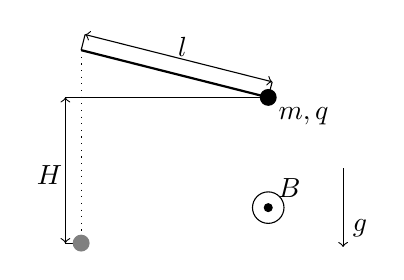
\begin{tikzpicture}
\newcommand{\x}{1.2*1.98}
\newcommand{\y}{-0.6}
\newcommand{\length}{{veclen(\x,\y)}}

\draw (\x,-2) circle (0.2) node [above right] {$B$};
\draw[fill=black] (\x, -2) circle (0.05);
\draw[->] (1.4*\x,-1.5) -- (1.4*\x,-2.5) node[above right] {$g$};

\draw[<->] (0.05,-0.05*\x/\y) -- (\x+0.05,\y-0.05*\x/\y);
\draw (0,0) -- (0.05,-0.05*\x/\y);
\draw (\x,\y) -- (\x+0.05,\y-0.05*\x/\y);
\draw[thick] (0,0) -- (\x,\y) node[below right] {$m,q$};
\draw[fill=black] (\x,\y) circle (0.1);
\node[above] at (\x/2+0.1,\y/2+0.1) {$l$};

\draw[<->] (-0.2,\y) -- (-0.2,-\length);
\draw (\x,\y) -- (-0.2,\y);
\draw (0,-\length) -- (-0.2,-\length);
\draw[dotted] (0,0) -- (0,-\length);
\draw[gray, fill=gray] (0,-\length) circle (0.1);
\node[left] at (0,-\length/2.5+\y) {$H~$};
\end{tikzpicture}}
\end{resizebox}
\end{center}
\fi
}

% Ü285
\ylDisplay{Silinder} % Ülesande nimi
{Tundmatu autor} % Autor
{lahtine} % Voor
{2007} % Aasta
{G 10} % Ülesande nr.
{10} % Raskustase
{
% Teema: Magnetism
\ifStatement
Pika ühtlase mittejuhtiva silindri pinnal on ühtlaselt jaotatud laeng pindtihedusega $\sigma$. Alguses asub silinder välises homogeenses magnetväljas induktsiooniga $B$, mis on suunatud piki silindri telge; silinder on paigal. Seejärel lülitatakse magnetväli välja. Kui suure pöörlemise nurkkiiruse omandab selle tulemusel silinder? Silindri aine tihedus on $\rho$, silindri raadius on $r$. 

\emph{Märkus}. Pöörleva silindri poolt tekitatav magnetväli lugeda tühiselt väikseks võrreldes välise väljaga
\fi
}

% Ü286
\ylDisplay{Elektronid} % Ülesande nimi
{Jaan Kalda} % Autor
{lõppvoor} % Voor
{2017} % Aasta
{G 10} % Ülesande nr.
{10} % Raskustase
{
% Teema: Magnetism
\ifStatement
Ruumipiirkonnas $x>-a$ ($a>0$) on homogeenne $z$-telje sihiline magnetväli induktsiooniga $B$. 
Koordinaatide alguspunktis on elektronide allikas, mis kiirgab elektrone võrdsel arvul
kõikidesse suundadesse (üle ruuminurga $4\pi$). Kõikide elektronide kiirus on $v$. Tasandis $x=-a$ on ekraan. Kui elektronid 
laenguga $e$ ja massiga $m$ põrkuvad vastu 
ekraani, siis on kokkupõrkepunktis näha helendust. Leidke helenduva laigu $y$-telje sihiline
läbimõõt tasandil $z = 0$ eeldusel, et vähemalt osa elektronidest jõuavad ekraanini.
Samal tasandil leida, kus kohas on laigu helenduse intensiivsus
kõige suurem. Milline on selle laigu $z$-telje sihiline pikkus tasandil $y=0$? 
\fi
}
\newpage\subsection{\protect\StrSubstitute{Staatika}{-}{ }}

% Ü287
\ylDisplay{Pendel} % Ülesande nimi
{Mihkel Heidelberg} % Autor
{piirkonnavoor} % Voor
{2008} % Aasta
{G 1} % Ülesande nr.
{1} % Raskustase
{
% Teema: Staatika
\ifStatement
Otsast kinnitatud varras saab pöörelda ümber horisontaaltelje ühes tasandis. Varda otsa on kinnitatud koormis massiga $m$. Varda pikkus on $l$. Varda kinnitusele mõjub hõõrdest tingitud pidurdav jõumoment $M$. Millistes nurkade vahemikes võib olla varras paigal (vt joonist)? Arvestada, et $mgl > M$.
\begin{center}
	\includegraphics[width=0.3\linewidth]{2008-v2g-01-yl}
\end{center}
\fi
}

% Ü288
\ylDisplay{Toru} % Ülesande nimi
{Tundmatu autor} % Autor
{lahtine} % Voor
{2007} % Aasta
{G 2} % Ülesande nr.
{2} % Raskustase
{
% Teema: Staatika
\ifStatement
Kaks inimest kannavad toru massiga $m = \SI{80}{kg}$ ja pikkusega $l = \SI{5}{m}$. Esimene inimene hoiab toru kaugusel $a = \SI{1}{m}$ toru otsast, teine aga hoiab toru teist otsa. Leida jõud, mida toru avaldab igale inimesele.
\fi
}

% Ü289
\ylDisplay{Nürinenud käärid} % Ülesande nimi
{Mihkel Kree} % Autor
{lõppvoor} % Voor
{2009} % Aasta
{G 1} % Ülesande nr.
{2} % Raskustase
{
% Teema: Staatika
\ifStatement
Juku asus hekikääridega õunapuult jämedat kuivanud oksa lõikama. Et aga käärid olid juba ammu nürinenud, polnud neist mingit abi. Enamgi veel, oks hakkas kääride kokkuvajutamise ajal terade vahel lausa libisema. Libisemine peatus hetkel, mil terade vaheline nurk oli kahanenud $\alpha$-ni. Kui suur oli hõõrdetegur oksa ja nürinenud lõiketera vahel?
\fi
}

% Ü290
\ylDisplay{Kuul} % Ülesande nimi
{Tundmatu autor} % Autor
{lahtine} % Voor
{2005} % Aasta
{G 3} % Ülesande nr.
{3} % Raskustase
{
% Teema: Staatika
\ifStatement
Metallist kuul asetseb lauaaugus, mille sügavus on 2 korda väiksem kuuli raadiusest (vt joonist). Kui suure laua kaldenurga $\alpha$ puhul kuul kukub august välja? 

\begin{center}
	\includegraphics[width=0.4\linewidth]{2005-lahg-03-yl}
\end{center}
\fi
}

% Ü291
\ylDisplay{Katus} % Ülesande nimi
{Ott Krikmann} % Autor
{piirkonnavoor} % Voor
{2005} % Aasta
{G 2} % Ülesande nr.
{3} % Raskustase
{
% Teema: Staatika
\ifStatement
Ühtlase lumekihiga kaetud katus on horisondi suhtes kaldu $\alpha = \SI{40}{\degree}$ nurga all. Katus on ristküliku kujuline ja laius harjast räästani mööda katuse pinda on $L$. Katuse ja lume vaheline hõõrdetegur on $\mu = \num{1}$. Katuse harjast hakkab lumekihi ja katuse vahele voolama vesi, mis muudab märja katuse ja lumekihi vahelise hõõrdeteguri nulliks. Kui vesi jõuab katuseharjast kaugusele $l$, hakkab lumekiht alla libisema. Leidke suhe $l/L$.
\fi
}

% Ü292
\ylDisplay{Kast kaubikus} % Ülesande nimi
{Oleg Košik} % Autor
{lõppvoor} % Voor
{2009} % Aasta
{G 2} % Ülesande nr.
{3} % Raskustase
{
% Teema: Staatika
\ifStatement
Kast massiga $m=\SI{15}{kg}$ on kinnitatud kaubiku tagaseina külge nööriga. Leida nööri pinge minimaalne võimalik väärtus äkkpidurduse ajal, kui kiirusega $v_0=\SI{45}{km/h}$ sõitev kaubik jääb seisma ajaga $t=\SI{5}{s}$. Hõõrdetegur kasti aluse ja kaubiku põranda vahel $\mu=\num{0,2}$, nurk nööri ja kaubiku tagaseina vahel $\alpha=\SI{45}{\degree}$. Lugeda, et pidurdamine oli ühtlane ja kast püsis kogu aeg paigal.
\begin{center}
	\includegraphics[width=0.5\linewidth]{2009-v3g-02-G_kast_kaubikus.eps}
\end{center}
\fi
}

% Ü293
\ylDisplay{Liivahunnik} % Ülesande nimi
{Roland Matt} % Autor
{piirkonnavoor} % Voor
{2011} % Aasta
{G 5} % Ülesande nr.
{3} % Raskustase
{
% Teema: Staatika
\ifStatement
Millisele pindalale on võimalik mahutada koonusekujuline liivahunnik, kui liiva ruumala on $V=\SI{50}{m^{3}}$ ja libisevate liivakihtide vaheline efektiivne hõõrdetegur $\mu=\num{0.4}$? Liivahunniku ja aluspinna hõõrdeteguri võib lugeda väga suureks.
\fi
}

% Ü294
\ylDisplay{Tormituul} % Ülesande nimi
{Mihkel Kree} % Autor
{lõppvoor} % Voor
{2011} % Aasta
{G 3} % Ülesande nr.
{4} % Raskustase
{
% Teema: Staatika
\ifStatement
Vaatleme tugeva külgtuule kätte jäänud veoautot lihtsustatult homogeense risttahukana. Auto laius on $a = \SI{2}{m}$, kõrgus $b = \SI{3}{m}$, pikkus
$c = \SI{5}{m}$. Missugune peaks olema hõõrdetegur rataste ja maapinna vahel, et piisavalt tugev külgtuul saaks auto tuulepoolsed rattad maast lahti kergitada?
\fi
}

% Ü295
\ylDisplay{Rõngas} % Ülesande nimi
{Taavi Pungas} % Autor
{piirkonnavoor} % Voor
{2014} % Aasta
{G 6} % Ülesande nr.
{4} % Raskustase
{
% Teema: Staatika
\ifStatement
Lae külge on nööriga, mille pikkus on $L$, kinnitatud kerge plastmassrõngas raadiusega $R$, mille küljes on omakorda raske metallist mutter. Mutrit saab mööda rõngast libistada. Rõnga ja mutri vaheline hõõrdetegur on $\mu$. Juku tahab mutrit mööda rõngast nihutades saavutada olukorda, kus mutri ja lae vahekaugus $h$ oleks võimalikult väike, aga süsteem püsiks veel ilma välise sekkumiseta tasakaalus. Leidke vähim vahekaugus $h\idx{min}$, mille Juku võib saavutada. Eeldage, et rõnga mass on mutri omaga võrreldes tühiselt väike.
\fi
}

% Ü296
\ylDisplay{Hammasrattad} % Ülesande nimi
{Siim Ainsaar} % Autor
{lõppvoor} % Voor
{2010} % Aasta
{G 4} % Ülesande nr.
{5} % Raskustase
{
% Teema: Staatika
\ifStatement
Fikseeritud telgedega hammasrattad raadiustega $r_1$ ja $r_2$ hambuvad ja on
ühendatud venimatu nööriga,
mis on mõlemale puutujaks. Esimest ratast pööratakse
jõumomendiga $M$. Kui suur on nööri pinge $T$?

\begin{center}
	\includegraphics{2010-v3g-04-joonis_hr_ipe.pdf}
\end{center}
\fi
}

% Ü297
\ylDisplay{Poldilõikur} % Ülesande nimi
{Mihkel Rähn} % Autor
{piirkonnavoor} % Voor
{2015} % Aasta
{G 7} % Ülesande nr.
{5} % Raskustase
{
% Teema: Staatika
\ifStatement
Leida, kui suurt jõudu avaldab poldilõikuri tera poldile (vt joonis), kui käepidemetele avaldatud jõud on $F = \SI{90}{N}$.
 \begin{center}
 \includegraphics[width=0.7\textwidth]{2015-v2g-07-poldiloikur}
 \end{center}
\fi
}

% Ü298
\ylDisplay{Kuul} % Ülesande nimi
{Tundmatu autor} % Autor
{lahtine} % Voor
{2006} % Aasta
{G 7} % Ülesande nr.
{6} % Raskustase
{
% Teema: Staatika
\ifStatement
Kasti tasasel põhjal asub kuul. Kasti põhi asub nurga all horisontaalsuuna suhtes. Kuuli hoiab tasakaalus kasti seina külge kinnitatud niit, mis on paralleelne kasti põhjaga (vt joonist). Kui suure maksimaalse nurga $\varphi$ võrra saab kasti kallutada, et kuul oleks veel tasakaalus? Hõõrdetegur kuuli ja kasti vahel on $\mu$.

\begin{center}
	\includegraphics[width=0.5\linewidth]{2006-lahg-07-yl}
\end{center}
\fi
}

% Ü299
\ylDisplay{Toru} % Ülesande nimi
{Aigar Vaigu} % Autor
{lõppvoor} % Voor
{2010} % Aasta
{G 5} % Ülesande nr.
{6} % Raskustase
{
% Teema: Staatika
\ifStatement
Kareda horisontaalselt kinnitatud toru (raadius $R$) peal tasakaalustatakse risttahukakujulist prussi. Leidke prussi paksus $L$, mille
korral prussi asend torul on stabiilne.

\emph{Märkus.} Võivad olla kasulikud väikeste nurkade korral kehtivad lähendused
$\sin\alpha\approx \alpha$ ja $\cos\alpha\approx 1-\alpha^2/2$, kus nurgad on radiaanides.
\fi
}

% Ü300
\ylDisplay{Klotsid} % Ülesande nimi
{Mihkel Rähn} % Autor
{piirkonnavoor} % Voor
{2014} % Aasta
{G 7} % Ülesande nr.
{6} % Raskustase
{
% Teema: Staatika
\ifStatement
Horisontaalsel laual asuva klotsi massiga $m_1$ peale on asetatud teine klots massiga $m_2$. Kahe klotsi vaheline seisuhõõrdetegur on $\mu_2$. Alumise klotsi ja laua vaheline liugehõõrdetegur on $\mu_1$. Leidke maksimaalne horisontaalne jõud $F$, millega võib alumist klotsi tõmmata, ilma et ülemine klots libiseks.
\fi
}

% Ü301
\ylDisplay{Polüspast} % Ülesande nimi
{Mihkel Rähn} % Autor
{lõppvoor} % Voor
{2014} % Aasta
{G 6} % Ülesande nr.
{6} % Raskustase
{
% Teema: Staatika
\ifStatement
Jäälõhesse kukkunud alpinisti väljatõmbamiseks on käepärastest vahenditest (kolm plokki ja nöörijupid) koostatud polüspast. Lihtsustatud joonisel on jämeda joonega märgitud põhiköis, mille ühes otsas on kukkunu ning teisest otsast vinnatakse. Plokid on peene joonega kujutatud nööri abil kinnitatud mittelibiseva sõlmega (joonisel täidetud ring) põhiköie külge. Leidke polüspasti ülekandetegur nii hõõrdumist arvestamata kui ka eeldusel, et hõõrdumine vähendab jõuülekannet igal plokil $35\percent$. Eeldage, et kõik jõud on vertikaalsed.

\begin{center}
\includegraphics[width=0.25\linewidth]{2014-v3g-06-Polyspast}
\end{center}
\fi
}

% Ü302
\ylDisplay{Kelk} % Ülesande nimi
{Andreas Valdmann} % Autor
{piirkonnavoor} % Voor
{2018} % Aasta
{G 9} % Ülesande nr.
{6} % Raskustase
{
% Teema: Staatika
\ifStatement
Juku läks sõpradega kelgutama. Teel tagasi istusid Juku kaks sõpra kelgule ja Juku üritas kelku horisontaalsel lumisel teel enda järel vedada. Kui suur on minimaalne kelgunööri nurk maapinnaga, mille korral on Jukul võimalik kelk liikuma tõmmata? Juku mass $m_1 = \SI{60}{kg}$ ja hõõrdetegur Juku saabaste ning lume vahel $\mu_1 = \SI{0.30}{}$. Kelgu mass koos Juku sõpradega $m_2 = \SI{110}{kg}$ ja hõõrdetegur kelgu ning lume vahel $\mu_2 = \SI{0.20}{}$.
\fi
}

% Ü303
\ylDisplay{Kuubik} % Ülesande nimi
{Riho Taba} % Autor
{piirkonnavoor} % Voor
{2007} % Aasta
{G 9} % Ülesande nr.
{7} % Raskustase
{
% Teema: Staatika
\ifStatement
Kuubik massiga $m = \SI{10}{kg}$ ning küljepikkusega $a = \SI{0,1}{m}$ lebab laual. Laua ja kuubiku vaheline hõõrdetegur on $\mu = \num{0,5}$. Kas kuubikut on võimalik käega teisele küljele ajada, avaldades vaid jõudu kuni $F = \SI{40}{N}$? Eeldada, et hõõrdetegur käe ja kuubiku vahel on väga suur ehk käsi ei libise. Raskusjõu kiirendus on $g = \SI{9,8}{m/s^2}$.
\fi
}

% Ü304
\ylDisplay{Kuulid} % Ülesande nimi
{Jaan Kalda} % Autor
{lahtine} % Voor
{2009} % Aasta
{G 9} % Ülesande nr.
{7} % Raskustase
{
% Teema: Staatika
\ifStatement
Kolm ühesuguse raadiusega kuuli $A$, $B$ ja $C$ on ühendatud kergete varraste abil võrdkülgseks kolmnurgaks $ABC$, mis lebab siledal (kuid nullist erineva hõõrdeteguriga) horisontaalpinnal. Kuuli $C$ lükatakse hästi aeglaselt nii, et selle kiirusvektor on kogu aeg risti sirgega $AC$. Kui kuul $A$ on piisavalt raske (st masside suhe $M_A/M_B$ on piisavalt suur), siis jääb kuul $A$ paigale. Millise suhte $M_A/M_B$ puhul hakkab kuul $A$ libisema?
\fi
}

% Ü305
\ylDisplay{Rõngas} % Ülesande nimi
{Jaan Kalda} % Autor
{lõppvoor} % Voor
{2011} % Aasta
{G 7} % Ülesande nr.
{7} % Raskustase
{
% Teema: Staatika
\ifStatement
Ebaühtlase massijaotusega traadist on tehtud rõngas, mis kujutab endast ringi raadiusega $R$. Selle rõnga massikese asub ringi keskpunktist
kaugusel $R/2$. Rõngas asetatakse horisontaalsele võllile rippuma. Milline peab
olema rõnga ja võlli vaheline hõõrdetegur $\mu$, et võlli aeglasel pöörlemisel rõngas
võllil ei libiseks?
\fi
}

% Ü306
\ylDisplay{Niidirull} % Ülesande nimi
{Mihkel Kree} % Autor
{lahtine} % Voor
{2013} % Aasta
{G 8} % Ülesande nr.
{7} % Raskustase
{
% Teema: Staatika
\ifStatement
\begin{wrapfigure}[6]{r}{3cm}
\vspace{-15pt}
\includegraphics[width=\linewidth]{2013-lahg-08-joonis_niidirull-crop}
\end{wrapfigure}

Silinder massiga $m$, millele on keritud õhuke niit, asetatakse kaldpinnale nurgaga $\alpha$.
Millise minimaalse jõuga $F\idx{min}$ tuleb nöörist hoida, et silinder paigale
jääks (vt joonist)? Hõõrdetegur pinna ja silindri vahel on nii suur, et
libisemist ei toimu.
\fi
}

% Ü307
\ylDisplay{Jalgrattur} % Ülesande nimi
{Andres Põldaru} % Autor
{lahtine} % Voor
{2014} % Aasta
{G 8} % Ülesande nr.
{7} % Raskustase
{
% Teema: Staatika
\ifStatement
Jalgrattur sõidab alla ühtlase kallakuga nõlvast. Kui ta vajutab pidureid täpselt nii kõvasti, et tagumine ratas on peaaegu õhku tõusmas, siis tema kiirus mäest alla sõites ei muutu. Jalgratturist ja rattast koosneva süsteemi massikese asub täpselt kahe ratta vahel kaugusel $h$ maapinnast, rataste telgede vahekaugus on $d$. Kui suur on nõlva ja horisontaalsihi vaheline nurk $\alpha$? Kui suur peab olema ratta ja kaldpinna vaheline hõõrdetegur $\mu$, et jalgrattur saaks kirjeldatud moel pidurdada?
\fi
}

% Ü308
\ylDisplay{Varras} % Ülesande nimi
{Siim Ainsaar} % Autor
{lõppvoor} % Voor
{2008} % Aasta
{G 9} % Ülesande nr.
{9} % Raskustase
{
% Teema: Staatika
\ifStatement
\begin{wrapfigure}[8]{r}{0.4\textwidth}
	\begin{center}
		\vspace{-25pt}
		\includegraphics[width=\linewidth]{2008-v3g-09-yl}
	\end{center}
\end{wrapfigure}
Peenike homogeenne varras toetub ühe otsaga vastu põrandat (hõõrdetegur varda otsa ja põranda vahel on $\mu$) ning küljega vastu libedat horisontaalset silindrit (hõõrdetegur on tühiselt väike), vt joonist. Silinder on liikumatult kinnitatud põranda külge, varras on risti silindri teljega ning moodustab põrandaga nurga $\alpha$. Millise varda pikkuse $l$ korral jääb varras sellisesse asendisse püsima?
\fi
}

% Ü309
\ylDisplay{Konn} % Ülesande nimi
{Taavi Pungas} % Autor
{lahtine} % Voor
{2010} % Aasta
{G 9} % Ülesande nr.
{9} % Raskustase
{
% Teema: Staatika
\ifStatement
\begin{wrapfigure}{r}{0.35\textwidth}
	\vspace{-1.8ex}
	\includegraphics[width=\linewidth]{2010-lahg-09-Red_eyed_tree_frog}
	\vspace{-4ex}
\end{wrapfigure}
Väike puukonn suudab ronida mööda seinu ja lagesid, luues enda ja seina vahele 
seinaga risti oleva tõmbejõu (nt iminappade tekitatud vaakumiga) ning vältides libisemist 
selle tagajärjel tekkiva hõõrdejõu abil.
Millise nurga all maapinna suhtes peab olema sein, et tal oleks end kõige raskem paigal hoida 
(mil libisemise vältimiseks vajalik seinaga risti olev jõud on maksimaalne)?
Hõõrdetegur seina ja konna vahel on $\mu$.
\fi
}

% Ü310
\ylDisplay{Torud} % Ülesande nimi
{Jaan Kalda} % Autor
{piirkonnavoor} % Voor
{2010} % Aasta
{G 10} % Ülesande nr.
{9} % Raskustase
{
% Teema: Staatika
\ifStatement
Põrandale asetatakse kõrvuti kaks ühesugust silindrilist toru --- paralleelselt ja küljetsi üksteist puutuvana. Kolmas samasugune toru asetatakse nende peale --- samuti paralleelselt, nõnda et see toetub kahele alumisele.
Milliseid tingimusi peavad rahuldama hõõrdetegur $\mu$ toru ja põranda vahel ning hõõrdetegur $k$ kahe toru vahel
selleks, et pealmine toru kahte alumist üksteisest eemale ei vajutaks?

\begin{center}
	\includegraphics[width=0.3\linewidth]{2010-v2g-10-torud.eps}
\end{center}
\fi
}

% Ü311
\ylDisplay{Tungraud} % Ülesande nimi
{Valter Kiisk} % Autor
{lõppvoor} % Voor
{2011} % Aasta
{G 10} % Ülesande nr.
{9} % Raskustase
{
% Teema: Staatika
\ifStatement
Joonisel on kujutatud lihtsa konstruktsiooniga tungraud,
mille keerme samm on \SI{3}{mm}. Tungrauale surub auto jõuga $F = \SI{5}{kN}$. Vaatleme hetke, millal $\alpha = \SI{40}{\degree}$. Tungraua mõõtmeid vaadake jooniselt.\\
\osa Kui suure jõuga tuleb auto tõstmiseks vända käepidemele mõjuda, kui jätta
arvestamata hõõrdumine kõigi libisevate pindade vahel?\\
\osa Kui hõõre oleks ka tegelikult tühiselt väike, siis ei püsiks tungraud üleskeeratud asendis: niipea, kui käepidemest lahti lasta, hakkaks see auto raskuse
mõjul pöörlema ja auto vajuks taas alla. Vastake eelmisele küsimusele eeldusel,
et hõõrdetegur on parajasti nii suur (st mitte suurem, kui hädapärast vaja),
et tungraud jääks üleskeeratud asendisse püsima.

\begin{center}
	\includegraphics[scale=0.9]{2011-v3g-10-tungraud}
\end{center}
\fi
}

% Ü312
\ylDisplay{Nöör rennis} % Ülesande nimi
{Stanislav Zavjalov} % Autor
{lahtine} % Voor
{2012} % Aasta
{G 9} % Ülesanne nr.
{9} % Raskustase
{
% Teema: Staatika
\ifStatement
\begin{wrapfigure}{r}{0.4\linewidth}
\includegraphics[width=\linewidth]{2012-lahg-09-n88r_ipe}
\end{wrapfigure}
Kaks plaati moodustavad V-kujulise horisontaalse renni. Mõlemad plaadid on
horisontaaltasapinna suhtes nurga $\theta$ all.
Rennis on jupp ühtlase
massijaotusega nööri pikkusega $L$, mis asub tervikuna renniga ristuvas tasandis
nii, et mõlema plaadiga puutub kokku sama palju nööri.
Renni põhja kohal ei toetu nöör enam pikkuse $fL$
ulatuses plaatidele. Leidke $f$, kui nöör on libisemise piiril. Hõõrdetegur nööri ja plaatide
vahel on $\mu = 1$.
\fi
}

% Ü313
\ylDisplay{Katus} % Ülesande nimi
{Jaan Kalda} % Autor
{lõppvoor} % Voor
{2017} % Aasta
{G 9} % Ülesande nr.
{9} % Raskustase
{
% Teema: Staatika
\ifStatement
Kaks jäika traadijuppi pikkusega $L$ on ühendatud otsapidi (nt niidiga seotud) nii, et nende otspunktid on kontaktis ja nende vaheline nurk saab takistuseta muutuda, moodustades V-kujulise figuuri. See traadist moodustis asetatakse horisontaalse libedapinnalise silindri peale nõnda, et tasakaaluasendis moodustub traadist \enquote{katus} (tagurpidi \enquote{V}) tipunurgaga $\alpha$. Massijaotus traadis on ühtlane, hõõre traadi ja silindri vahel puudub. a) Milline on silindri raadius $R$? b) Milline võrratus peab olema rahuldatud, et see asend oleks stabiilne (uurida stabiilsust vaid \enquote{katuse} kui terviku pöördumise suhtes, eeldades et traatidevaheline nurk ei muutu)?
\fi
}

% Ü314
\ylDisplay{Platvorm} % Ülesande nimi
{Jaan Kalda} % Autor
{lõppvoor} % Voor
{2005} % Aasta
{G 10} % Ülesande nr.
{10} % Raskustase
{
% Teema: Staatika
\ifStatement
\begin{wrapfigure}[9]{r}{0.3\textwidth}
	\begin{center}
		\vspace{-20pt}
		\includegraphics[width=\linewidth]{2005-v3g-10-yl}
	\end{center}
\end{wrapfigure}
Siledas põrandas on pöörlev ringikujuline platvorm (joonisel pealtvaates, hall), mis on samast materjalist nagu põrandki (joonisel valge). Põranda ja platvormi ülemine pind on samal horisontaaltasandil. Kolm ühesugust keha ühendatakse kergete varraste abil kolmnurgaks ning asetatakse sedasi, et kaks keha asuvad platvormil punktides $A$ ja $B$ (vt joonist). Vardad ei puuduta ei põrandat, ega platvormi.\\
\osa Kui kolmas keha lebaks põrandal punktis $C$, kas siis kolmnurk hakkaks põranda suhtes liikuma või jääks paigale? Põhjendage vastust.\\
\osa Märkige joonisel selline punktihulk $X$, kus võiks asuda kolmas keha nii, et kolmnurk jääks põranda suhtes paigale.

\emph{Märkus}. Kolmnurga külgede $AC$ ja $BC$ pikkusi võib muuta. Seega, kui kolmas keha asub punktis $D \in X$, siis üldjuhul $|AD| \neq |AC|$ ja $|BD| \neq |BC|$.
\fi
}

% Ü315
\ylDisplay{Niidiga hantel} % Ülesande nimi
{Jaan Kalda} % Autor
{lõppvoor} % Voor
{2015} % Aasta
{G 9} % Ülesande nr.
{10} % Raskustase
{
% Teema: Staatika
\ifStatement
\begin{wrapfigure}{r}{0.23\textwidth}%
\vspace{-5 pt}%
\includegraphics[width=0.23\textwidth]{2015-v3g-09-hantel}%
\vspace{-15 pt}%
\end{wrapfigure}
Horisontaalpinnal lebab hantel, mis koosneb kaalutust vardast pikkusega $l=4a$ ning selle otstele kinnitatud kahest ühesuguse massi ja hõõrdeteguriga väikesest klotsist. Varda külge kaugusele $a$ ühest klotsist on seotud pikk niit. Algul on niidi suund horisontaalne ja risti vardaga. Niiti aeglaselt tõmmates hakkab hantel pöörduma, sest alguses nihkub vaid üks klots. Milline on nurk $\alpha$ varda ja niidi vahel siis, kui ka teine klots nihkuma hakkab?

\fi
}
\newpage\subsection{\protect\StrSubstitute{Taevamehaanika}{-}{ }}

% Ü316
\ylDisplay{Satelliit} % Ülesande nimi
{Mihkel Pajusalu} % Autor
{piirkonnavoor} % Voor
{2011} % Aasta
{G 2} % Ülesande nr.
{1} % Raskustase
{
% Teema: Taevamehaanika
\ifStatement
Satelliit tiirleb ringikujulisel orbiidil (raadiusega $r=\SI{7000}{\kilo\metre}$) ümber maakera, kusjuures satelliidi orbiit on samas tasapinnas Maa orbiidiga ümber Päikese. Kui suure osa ajast veedab satelliit keskmiselt Maa varjus? Maa läbimõõt on $R=\SI{6378}{\kilo\metre}$. Päikeselt tulevad kiired võib lugeda paralleelseteks ja Maa liikumise ühe satelliidi orbiiditaalperioodi jooksul tühiseks.
\fi
}

% Ü317
\ylDisplay{Väike prints} % Ülesande nimi
{Urmo Visk} % Autor
{piirkonnavoor} % Voor
{2009} % Aasta
{G 1} % Ülesande nr.
{2} % Raskustase
{
% Teema: Taevamehaanika
\ifStatement
Väike Prints elab sfäärilisel asteroidil B-612. Jalutades märkas väike prints, et mida kiiremini ta kõnnib, seda kergemaks ta muutub. Kui väike prints jooksis piki asteroidi ekvaatorit kiirusega $v = \SI{6}{m/s}$, siis muutus ta kaalutuks ja hakkas asteroidi pinna kohal hõljuma. Kui suur on asteroidi raadius $R$? Eeldame, et asteroid ei pöörle. Asteroidi tihedus on $\rho = \SI{5200}{kg/m^3}$, gravitatsioonikonstant $G = \SI{6.67e-11}{m^3.kg^{-1}.s^{-2}}$.
\fi
}

% Ü318
\ylDisplay{Maa pöörlemisperiood} % Ülesande nimi
{Eero Vaher} % Autor
{piirkonnavoor} % Voor
{2014} % Aasta
{G 3} % Ülesande nr.
{2} % Raskustase
{
% Teema: Taevamehaanika
\ifStatement
Keskmiseks päikeseööpäevaks ehk tavatähenduses ööpäevaks nimetatakse keskmist perioodi, mille jooksul Päike näib Maaga seotud vaatleja jaoks tegevat taevas täisringi. Keskmise päikeseööpäeva pikkuseks on \SI{24}{\hour} ehk \SI{86400}{\second}. Maal kulub ühe tiiru tegemiseks ümber Päikese \SI{365.256}{} keskmist päikeseööpäeva. Maa pöörlemissuund ümber oma telje ühtib selle tiirlemissuunaga Päikese ümber. Leidke nende andmete põhjal Maa pöörlemisperiood sekundi täpsusega. 
\fi
}

% Ü319
\ylDisplay{Eksinud satelliit} % Ülesande nimi
{Tundmatu autor} % Autor
{lahtine} % Voor
{2009} % Aasta
{G 5} % Ülesande nr.
{3} % Raskustase
{
% Teema: Taevamehaanika
\ifStatement
Sidesatelliidid paiknevad geostatsionaarsel orbiidil --- st niisugusel ringorbiidil, mille raadius ja suund on sellised, et satelliit püsib maapinna suhtes kogu aeg paigal. Ühe sidesatelliidi saatmisel aga esines viga, nii et ta saavutas küll õige kõrguse, kuid ringorbiidi suund sattus juhuslik. Milline on suurim võimalik suhteline kiirus, millega võib selliselt \enquote{eksinud} satelliit kokku põrkuda mõne teise sidesatelliidiga? Maa raadius on $R = \SI{6400}{km}$, raskuskiirendus maapinnal $g = \SI{9,8}{m/s^2}$.
\fi
}

% Ü320
\ylDisplay{Orbiit} % Ülesande nimi
{Mihkel Pajusalu} % Autor
{lahtine} % Voor
{2014} % Aasta
{G 3} % Ülesande nr.
{3} % Raskustase
{
% Teema: Taevamehaanika
\ifStatement
Taevakehad tiirlevad teatavasti elliptilistel orbiitidel. Ka Kuu orbiit ümber Maa on elliptiline. Kui Kuu kõige väiksem kaugus Maa-Kuu süsteemi massikeskmest (mille selles ülesandes võib lugeda ühtivaks Maa keskpunktiga) on $r_{1}=\SI{360000}{km}$ ja orbitaalkiirus sellel kaugusel on $v_1=\SI{1.1}{km/s}$, siis kui suur on ligikaudu suurim kaugus Maa ja Kuu vahel? Maa massiks võtta $M=\SI{6.0e24}{kg}$ ja gravitatsioonikonstandiks $G=\SI{6.7e-11}{\newton\metre\squared\per\kilo\gram\squared}$.
\fi
}

% Ü321
\ylDisplay{Päikese tihedus} % Ülesande nimi
{Eero Vaher} % Autor
{piirkonnavoor} % Voor
{2013} % Aasta
{G 6} % Ülesande nr.
{4} % Raskustase
{
% Teema: Taevamehaanika
\ifStatement
Leidke Päikese keskmine tihedus $\varrho$. Maa
tiirlemisperiood on $T=1$~aasta, gravitatsioonikonstant 
$G=\SI{6.7e-11}{N m^2/kg^2}$, Maa kaugus Päikesest $R=\SI{1.5e11}{m}$, Päikese nurkläbimõõt Maalt vaadatuna on
$\alpha=\SI{0,54}{\degree}$ (see on nurk, mis moodustub kahe kiire vahel, mis on tõmmatud
vaatleja silma juurest Päikese diameetri otspunktide juurde).
\fi
}

% Ü322
\ylDisplay{Ühendatud satelliidid} % Ülesande nimi
{Eero Vaher} % Autor
{piirkonnavoor} % Voor
{2018} % Aasta
{G 6} % Ülesande nr.
{4} % Raskustase
{
% Teema: Taevamehaanika
\ifStatement
Kaks satelliiti, mõlemad massiga $m$, tiirlevad ümber planeedi massiga $M\gg m$ ringorbiitidel raadiustega $R_1$ ning $R_2=2R_1$. Satelliidid on omavahel ühendatud tühise massiga pinges trossiga pikkusega $R_1$, mille tõttu on mõlema satelliidi tiirlemisperiood $T$. Mitu korda on satelliitide joonkiirused $v_1$ ja $v_2$ suuremad või väiksemad joonkiirustest $v'_1$ ja $v'_2$, millega satelliidid tiirleksid oma orbiitidel trossi puudumisel?
\fi
}

% Ü323
\ylDisplay{Satelliit} % Ülesande nimi
{Eero Vaher} % Autor
{lõppvoor} % Voor
{2013} % Aasta
{G 5} % Ülesande nr.
{5} % Raskustase
{
% Teema: Taevamehaanika
\ifStatement
Geostatsionaarseks orbiidiks nimetatakse sellist orbiiti, millel asuv satelliit
Maa suhtes ei liigu. Kui suur on maa-ala, mida sellisel orbiidil olevalt
satelliidilt jälgida saab? Vastuseks esitage selle maa-ala läbimõõt mõõdetuna
mööda Maa pinda. Gravitatsioonikonstant $G=\SI{6.7e-11}{N \cdot m^2/kg^2}$, Maa
mass $M=\SI{6,0e24}{kg}$, Maa raadius $r=\SI{6400}{km}$, Maa
pöörlemisperiood $t=\SI{24}{h}$.
\fi
}

% Ü324
\ylDisplay{Kosmosejaam} % Ülesande nimi
{Oleg Košik} % Autor
{lõppvoor} % Voor
{2005} % Aasta
{G 9} % Ülesande nr.
{6} % Raskustase
{
% Teema: Taevamehaanika
\ifStatement
Joonisel on toodud ringorbiidil liikuva rahvusvahelise kosmosejaama trajektoor maapinna kohal (Maa keskpunktist kosmosejaamani tõmmatud sirge ja maapinna lõikepunkti jälg). Hinnake selle abil kosmosejaama kõrgust maapinnast. Maa raadius $R = \SI{6380}{km}$, raskuskiirendus maapinnal $g = \SI{9,8}{m/s^2}$.

\begin{center}
	\includegraphics[width=\linewidth]{2005-v3g-09-yl}
\end{center}
\fi
}

% Ü325
\ylDisplay{Kuukaabel} % Ülesande nimi
{Siim Ainsaar} % Autor
{piirkonnavoor} % Voor
{2009} % Aasta
{G 10} % Ülesande nr.
{8} % Raskustase
{
% Teema: Taevamehaanika
\ifStatement
Oletame, et Maa ja Kuu on ühendatud sirge homogeense mõlema suhtes radiaalse kaabliga.\\
\osa Mitu korda on Maa poolt kaablile avaldatav ras\-kus\-jõud suurem
Kuu-pool\-sest?\\
\osa Maa pinnal asuv kaabli kinnitus sellele vertikaalsihis jõudu ei avalda.
Kui kõrgel Kuu kohal asub punkt, kus pisut liiga nõrk kaabel katkeks?

Lugegem taevakehad paigalseisvaiks.
Maa raadius $r_M=\SI{6370}{km}$, Kuu raadius $r_K=\SI{1740}{km}$,
Maa mass $m_M=\SI{5,97e24}{kg}$, Kuu mass $m_K=\SI{7,35e22}{kg}$, taevakehade keskmete vahekaugus $D=\SI{3,80e5}{km}$.
%, gravitatsioonikonstant $G = \unit{6,67}{\newton \cdot
%\squaren\meter \per \squaren\kilogram}$.
%Kaabli joontihedus olgu $\lambda=\unit{7850}{\kilo\gram \per \meter}$.

\emph{Abivalem}. Kui kaablit tõmbaks Maa üksi ning otspunktide kaugused Maa
tsentrist oleksid $a$ ja $b$, mõjuks sellele raskusjõud $G m_M \lambda
\left( \tfrac1a - \tfrac1b \right)$,
kus $G$ on gravitatsioonikonstant ning $\lambda$ kaabli joontihedus (ühikuga \si{kg/m}).
\fi
}

% Ü326
\ylDisplay{Satelliidid} % Ülesande nimi
{Mihkel Kree} % Autor
{lõppvoor} % Voor
{2010} % Aasta
{G 7} % Ülesande nr.
{9} % Raskustase
{
% Teema: Taevamehaanika
\ifStatement
2009. aasta veebruaris põrkasid Siberi kohal 780 kilomeetri kõrgusel kokku USA ja Venemaa satelliidid. Pidades silmas, et ümber Maa tiirleb juba tuhandeid satelliite ning nende kõigi orbiite pole seetõttu võimalik omavahel koordineerida, hinnake mitme aasta tagant keskeltläbi niisugused juhuslikud kokkupõrked aset leiavad. Oma lahenduses kasutage järgmisi hinnanguid ja lähendusi: maalähedaste satelliitide arv $N=\num{2500}$; orbiidid jäävad maapinnast kõrguste vahemikku $h_1=\SI{200}{km}$ kuni $h_2=\SI{2000}{km}$ ning satelliidid on jaotunud selles kihis ühtlase ruumtihedusega; tüüpilise satelliidi ristlõikepindala $S=\SI{10}{m^2}$. Maa raadius $R=\SI{6400}{km}$, raskuskiirendus maapinnal $g=\SI{10}{m/s^2}$.
\fi
}
\newpage\subsection{\protect\StrSubstitute{Termodünaamika}{-}{ }}

% Ü327
\ylDisplay{Balloon} % Ülesande nimi
{Jaan Susi} % Autor
{lõppvoor} % Voor
{2005} % Aasta
{G 3} % Ülesande nr.
{1} % Raskustase
{
% Teema: Termodünaamika
\ifStatement
Suletud balloon ruumalaga $V = \SI{10}{l}$ oli täidetud veega temperatuuril $t_0 = \SI{0}{\celsius}$. Samal temperatuuril külmutati vesi jääks, mille tulemusena ballooni kest venis välja ja vesi avaldas kogu jäätumise protsessi käigus balloonile rõhku $p = \SI{5e7}{Pa}$.

Leida balloonis olnud vee ($\mathrm{H_2O}$) siseenergia muut koos märgiga. Jää tihedus $\rho_j = \SI{900}{kg/m^3}$ ja sulamissoojuseks antud rõhul $\lambda = \SI{317}{kJ/kg}$. Jää ja vee kokkusurutavust mitte arvestada. 
\fi
}

% Ü328
\ylDisplay{Kütteklaas} % Ülesande nimi
{Jaak Kikas} % Autor
{lõppvoor} % Voor
{2007} % Aasta
{G 1} % Ülesande nr.
{1} % Raskustase
{
% Teema: Termodünaamika
\ifStatement
Ruumide soojendamiseks kasutatava elektriliselt köetava klaasi pind on kaetud õhukese valgust läbilaskva elektrit juhtiva kihiga, mille vastasservadele rakendatakse elektriline pinge (vool kulgeb mööda klaasi pinda). Kuidas suhtuvad sellisest klaasist valmistatud ristkülikukujuliselt aknalt eralduvad soojusvõimsused $P_H$ ja $P_V$ sama pinge rakendamisel vastavalt klaasi horisontaalsete ($P_H$) ja vertikaalsete ($P_V$) servade vahel? Akna horisontaalmõõde $a = \SI{0,5}{m}$ ja vertikaalmõõde $b = \SI{1}{m}$.
\fi
}

% Ü329
\ylDisplay{Jääkuul} % Ülesande nimi
{Urmo Visk} % Autor
{piirkonnavoor} % Voor
{2008} % Aasta
{G 4} % Ülesande nr.
{1} % Raskustase
{
% Teema: Termodünaamika
\ifStatement
Õhukeste seintega jääst kera sees on õhk. Algselt on jääkera külmkapis temperatuuril $t_0 = \SI{-9}{\celsius}$ ning õhurõhk tema sees võrdub välisrõhuga $p_0 = \SI{105}{kPa}$. Kera tõstetakse külmikust välja tuppa, kus see hakkab soojenema. Kera sein on nii õhuke, et maksimaalne ülerõhk (st. sise- ja välisrõhkude vahe), mida ta purunemata talub on $\Delta p = \num{0,2}p_0$. Mis juhtub enne, kas kera hakkab sulama või ta puruneb ülerõhu tõttu? Kuuli soojenemine lugeda nii aeglaseks, et igal ajahetkel võib lugeda õhu temperatuuri tema sees ning seinte sise- ja välispinna temperatuurid võrdseks.
\fi
}

% Ü330
\ylDisplay{Küttesüsteem} % Ülesande nimi
{Tundmatu autor} % Autor
{piirkonnavoor} % Voor
{2011} % Aasta
{G 3} % Ülesande nr.
{1} % Raskustase
{
% Teema: Termodünaamika
\ifStatement
Küttesüsteem täidetakse $t_1=\SI{10}{\celsius}$ temperatuuriga veega. Kui palju peab paisupaagis olema vaba ruumi, et kütmisel avatud paisupaagist vesi välja ei voolaks? Küttesüsteemis on $V_1=\SI{250}{}$ liitrit vett ja tööolukorras on selle keskmine temperatuur $t_2=\SI{63}{\celsius}$. Vee ruumpaisumistegur on $\beta=3\times 10^{-4}K^{-1}$. Vedeliku ruumala mingil temperatuuril avaldub kujul $V=V_{0}(1+\beta t)$, kus $t$ on vedeliku temperatuur Celsiuse kraadides, ning $V_{0}$ on vedeliku ruumala temperatuuril \SI{0}{\celsius}.
\fi
}

% Ü331
\ylDisplay{Vee jäätumine} % Ülesande nimi
{Jaak Kikas} % Autor
{lahtine} % Voor
{2012} % Aasta
{G 1} % Ülesanne nr.
{1} % Raskustase
{
% Teema: Termodünaamika
\ifStatement
\SI{0,5}{\kilo\gram} jääkuubikuid asetati \SI{1}{l} vette algtemperatuuriga
\SI{0}{\celsius}. Milline peab olema jää algtemperatuur, et kogu vesi jäätuks?
Jää sulamissoojus on \SI{330}{\kilo\joule\per\kilo\gram}, erisoojus
\SI{2,1}{\kilo\joule\per(\kilogram.\celsius)}. Soojusvahetust keskkonnaga ei
toimu.
Vee tihedus $\rho = \SI{1000}{kg/m^3}$.
\fi
}

% Ü332
\ylDisplay{Veepudel} % Ülesande nimi
{Koit Timpmann} % Autor
{piirkonnavoor} % Voor
{2013} % Aasta
{G 2} % Ülesande nr.
{1} % Raskustase
{
% Teema: Termodünaamika
\ifStatement
Külma ilmaga oli autosse ununenud \num{2,0}-liitrine täis veepudel. Auto juurde tulnud
autojuht Koit ei uskunud oma silmi: temperatuur autos oli \SI{-3}{\celsius},
aga vesi pudelis ei olnud külmunud. Koidule tuli meelde, et ta oli kunagi
kuulnud, et väga puhas vedelik võib olla vedelas olekus ka allpool
tahkumistemperatuuri. Selle kontrollimiseks võttis ta pudeli ja raputas seda
ning suhteliselt kiiresti muutus selles osa veest jääks. Mitu grammi jääd tekkis
pudelisse? Vee erisoojus $c = \SI{4200}{\joule\per(\kilogram \cdot \celsius)}$
ja tihedus $\varrho = \SI{1000}{\kilogram\per\meter\cubed}$, jää
sulamissoojus $\lambda = \SI{340}{ kJ/kg}$. 
\fi
}

% Ü333
\ylDisplay{Ringprotsess} % Ülesande nimi
{Riho Taba} % Autor
{piirkonnavoor} % Voor
{2006} % Aasta
{G 2} % Ülesande nr.
{2} % Raskustase
{
% Teema: Termodünaamika
\ifStatement
Kas joonisel kujutatud ringprotsessil on ideaalse gaasi töö positiivne või negatiivne? Põhjendada vastust.

\begin{center}
	\includegraphics[width=0.4\linewidth]{2006-v2g-02-yl}
\end{center}
\fi
}

% Ü334
\ylDisplay{Vedelike segamine} % Ülesande nimi
{Aleksei Vlassov} % Autor
{piirkonnavoor} % Voor
{2007} % Aasta
{G 3} % Ülesande nr.
{2} % Raskustase
{
% Teema: Termodünaamika
\ifStatement
Kahe erineva vedeliku segamisel ruumalade suhtega $1 : 1$ tekib segu temperatuuriga $t_3 = \SI{42}{\celsius}$. Milline oleks segu temperatuur, kui ruumalade suhe oleks $2 : 1$? Vedelike temperatuurid on vastavalt $t_1 = \SI{27}{\celsius}$ ning $t_2 = \SI{47}{\celsius}$.
\fi
}

% Ü335
\ylDisplay{Tulehõõrumine} % Ülesande nimi
{Jaak Kikas} % Autor
{piirkonnavoor} % Voor
{2008} % Aasta
{G 3} % Ülesande nr.
{2} % Raskustase
{
% Teema: Termodünaamika
\ifStatement
Jõuga $F$ otsapidi vastu tasast pinda surutud toru pöörleb sagedusega $f$. Toru läbimõõt on $D$ ja seina paksus $d \ll D$. Toru otspind on risti toru teljega, hõõrdetegur toru ja tasapinna vahel on $\mu$. Kui palju soojusenergiat vabaneb ajavahemiku $\Delta t$ jooksul?

\begin{center}
	\includegraphics[width=0.3\linewidth]{2008-v2g-03-yl}
\end{center}
\fi
}

% Ü336
\ylDisplay{Termos} % Ülesande nimi
{Urmo Visk} % Autor
{piirkonnavoor} % Voor
{2009} % Aasta
{G 3} % Ülesande nr.
{2} % Raskustase
{
% Teema: Termodünaamika
\ifStatement
Termoses, mis on ümbritsevatest kehadest soojuslikult isoleeritud, on $m_1 = \SI{300}g$ vett temperatuuriga $t_1 = \SI{20}{\celsius}$. Sellele lisatakse $m_2 = \SI{600}g$ vett temperatuuriga $t_2 = \SI{80}{\celsius}$. Pärast soojusliku
tasakaalu saabumist mõõdeti vee temperatuuriks $T_1$. Järgmisel korral oli
samas anumas alguses $m_2 = \SI{600}g$ vett temperatuuriga $t_2 = \SI{80}{\celsius}$ ja sellele lisati $m_1 = \SI{300}g$ vett temperatuuriga $t_1 = \SI{20}{\celsius}$. Nüüd mõõdeti vee temperatuuriks soojusliku tasakaalu saabumise järel $T_2 = T_1+\SI{2}{\celsius}$. Kui
suur on termose materjali erisoojus? Tühja termose mass on $m = \SI{140}g$ ja vee erisoojus $c = \SI{4200}{J/kg.C}$.

\fi
}

% Ü337
\ylDisplay{Rauatükk} % Ülesande nimi
{Oleg Košik} % Autor
{lahtine} % Voor
{2010} % Aasta
{G 2} % Ülesande nr.
{2} % Raskustase
{
% Teema: Termodünaamika
\ifStatement
Anumasse, milles oli $V=\SI{1}{l}$ vett temperatuuril $t_1=20\celsius$,
visati rauatükk massiga $m=\SI{100}{g}$ temperatuuril $t_0=500\celsius$. Osa
veest aurustus. Mõne aja pärast mõõdeti vee temperatuuriks
$t_2=24\celsius$. Kui palju vett aurustus välja? Vee erisoojus
$c_1=\SI{4200}{J/(kg\cdot\celsius)}$, aurustumissoojus $L=\SI{2,26 e6}{J/kg}$ ja
tihedus $\rho=\SI{1000}{kg/m^3}$; raua
erisoojus $c_2=\SI{460}{J/(kg\cdot\celsius)}$. Anum on tühise soojusmahtuvusega ning väliskeskkonnast
hästi isoleeritud.
\fi
}

% Ü338
\ylDisplay{Jõhvikad} % Ülesande nimi
{Urmo Visk} % Autor
{piirkonnavoor} % Voor
{2010} % Aasta
{G 2} % Ülesande nr.
{2} % Raskustase
{
% Teema: Termodünaamika
\ifStatement
Keevasse vette kallatakse külmutatud jõhvikaid. Vee temperatuur langes väärtuseni $t=\SI{89}{\celsius}$.
Mitu korda oli vee mass suurem jõhvikate massist? Kuna jõhvikad oli väikesed ja sulasid väga kiiresti, siis
võib vee soojusvahetuse ümbritseva keskkonnaga arvestamata jätta. Jõhvikate algtemperatuur oli
$t_2=\SI{-18}{\celsius}$. Jää erisoojus $c_j=\SI{2100}{J/(kg.C)}$, vee erisoojus $c_v=\SI{4200}{J/(kg.\celsius)}$, jää sulamissoojus $L=\SI{330}{kJ/kg}$. Jõhvikate suure veesisalduse tõttu võib need jääna käsitleda.
\fi
}

% Ü339
\ylDisplay{Vesi} % Ülesande nimi
{Taavi Pungas} % Autor
{lõppvoor} % Voor
{2011} % Aasta
{G 1} % Ülesande nr.
{2} % Raskustase
{
% Teema: Termodünaamika
\ifStatement
Avatud termoses on vesi temperatuuril $t_0 = \SI{100}{\celsius}$. Sellest \SI{1}{\%}
aurustub. Hinnata, kui palju muutub termosesse jäänud vee temperatuur $t$.
Vee erisoojus $c_v = \SI{4,2}{kJ.kg^{-1}.K^{-1}}$, veeauru erisoojus $c_a = \SI{1,9}{kJ.kg^{-1}.K^{-1}}$ ning
vee aurustumissoojus temperatuuril \SI{100}{\celsius} on $L = \SI{2,26}{MJ/kg}$. Eeldada, et termose seinte kaudu soojuskadusid ei ole.
\fi
}

% Ü340
\ylDisplay{Hõõrdkeevitus} % Ülesande nimi
{Ants Remm} % Autor
{lõppvoor} % Voor
{2012} % Aasta
{G 1} % Ülesande nr.
{2} % Raskustase
{
% Teema: Termodünaamika
\ifStatement
Suhteliselt uus keevitustehnoloogia on hõõrdkeevitus. See seisneb selles, et üks
liidetavatest detailidest pannakse pöörlema ning surutakse vastu teist. Kui
tekkinud soojus on detailid peaaegu sulamistemperatuurini kuumutanud, jäetakse
pöörlev detail seisma ning suure rõhu all moodustub side. Vaatame olukorda, kus
kaks vasest torujuppi tahetakse kokku keevitada. Leidke, kui suure jõuga peab
pöörlemise ajal torusid kokku suruma, et tekiks piisavalt suur soojushulk
$\Delta t = \SI{6}{s}$ jooksul. Toru pöörlemiskiirus on $f = 1200$ pööret
minutis. Lihtsustatult võib eeldada, et mõlema toru otsast kuumeneb ühtlaselt $l
= \SI{0,5}{cm}$ pikkune jupp. Torude diameeter on $D = \SI{8}{cm}$, seina paksus
$d = \SI{5}{mm}$. Torud on alguses toatemperatuuril $T_0 = \SI{20}{^\circ C}$.
Liitumine toimub temperatuuril $T_1 = \SI{810}{^\circ C}$. Vase hõõrdetegur
iseendaga on $\mu = 0,96$, tihedus $\rho = \SI{8,9}{\frac{g}{cm^3}}$ ning
erisoojus $c = \SI{390}{\frac{J}{kg \cdot \celsius}}$. Soojuskadudega ümbritsevasse
keskkonda mitte arvestada.
\fi
}

% Ü341
\ylDisplay{Münt jääs} % Ülesande nimi
{Erkki Tempel} % Autor
{piirkonnavoor} % Voor
{2015} % Aasta
{G 3} % Ülesande nr.
{2} % Raskustase
{
% Teema: Termodünaamika
\ifStatement
Jäätüki sisse on jäätunud münt massiga $m_m=\SI{10}{g}$ ja tihedusega $\rho_m=\SI{8900}{kg/m^3}$. Jäätüki ja mündi temperatuur on \SI{0}{\celsius}. Jäätükk ilma mündita kaalub $m_j=\SI{130}{g}$. See jäätükk visatakse anumasse, milles on $V_v=\SI{400}{ml}$ vett algtemperatuuriga $T$. Kui suur peab olema vee minimaalne algtemperatuur $T$, et jäätükk koos mündiga vajuks pärast soojusliku tasakaalu saabumist põhja? Soojusvahetust väliskeskkonnaga mitte arvestada. Vee erisoojus $c=\SI{4200}{J/ (kg\cdot\celsius)}$ ning jää sulamissoojus $\lambda=\SI{330}{kJ/kg}$. Jää tihedus $\rho_j=\SI{900}{kg/m^3}$ ja vee tihedus $\rho_v=\SI{1000}{kg/m^3}$.
\fi
}

% Ü342
\ylDisplay{Soojusvaheti} % Ülesande nimi
{Kaur Aare Saar} % Autor
{lõppvoor} % Voor
{2016} % Aasta
{G 1} % Ülesande nr.
{2} % Raskustase
{
% Teema: Termodünaamika
\ifStatement
Tagasivoolu soojusvahetis jahutatakse sissetulevat naftat temperatuuriga $T_{n}=\SI{90}{\celsius}$ temperatuurini $T_{0}=\SI{20}{\celsius}$. 
Jahutusvesi liigub soojusvahetis vastupidises suunas naftaga ja siseneb soojusvahetisse temperatuuriga $T_{v}=\SI{10}{\celsius}$.
Vesi liigub kiirusega $v_{v}=\SI{6}{\m^3\per\minute}$ 
ja nafta liigub kiirusega $v_{n}=\SI{15}{\m^3\per\minute}$. 
Leidke, millise temperatuuriga väljub soojusvahetist vesi? Vee erisoojus $c_{v}=\SI{4200}{\joule\per\kilogram\per\celsius}$ 
ja nafta erisoojus $c_{n}=\SI{1800}{\joule\per\kilogram\per\celsius}$. Vee tihedus $\rho_{v}=\SI{1000}{\kilogram\per\metre\cubed}$ ja nafta tihedus $\rho_{n}=\SI{850}{\kilogram\per\metre\cubed}$.
\fi
}

% Ü343
\ylDisplay{Kastmisvesi} % Ülesande nimi
{Urmo Visk} % Autor
{piirkonnavoor} % Voor
{2008} % Aasta
{G 5} % Ülesande nr.
{3} % Raskustase
{
% Teema: Termodünaamika
\ifStatement
Päikeselisel suvepäeval langeb päikesekiirtega risti olevale ühe ruutmeetrisele pinnale ühes sekundis keskmiselt $\varepsilon = \SI{0,5}{kJ/(s.m^2}$) energiat. Kastmisvett soojendatakse pilgeni täis valatud õhukeseseinalises kerakujulises anumas raadiusega $R = \SI{0,5}{m}$. Eeldada, et veeanum on päeva jooksul täielikult valgustatud. Kastmisvee temperatuur päikesetõusu ajal kell 4.30 oli $t_0 = \SI{16}{\celsius}$. Kui suur on kastmisvee temperatuur päikeseloojangu ajal kell 22.30? Vee erisoojus on $c = \SI{4200}{J/(kg.\celsius}$), tihedus $\rho = \SI{1}{kg/dm^3}$. Eeldada, et anum neelab kogu pealelangeva päikesevalguse energia ning, et kogu päikesevalguse energia läheb kastmisvee soojendamiseks. Soojusvahetus kastmisvee ja keskkonna vahel lugeda tühiseks.
\fi
}

% Ü344
\ylDisplay{Küttesüsteem} % Ülesande nimi
{Oleg Košik} % Autor
{piirkonnavoor} % Voor
{2012} % Aasta
{G 2} % Ülesande nr.
{3} % Raskustase
{
% Teema: Termodünaamika
\ifStatement
Talvel siseneb koolimaja küttesüsteemi vesi algtemperatuuriga $t_0=\SI{60}{\celsius}$
ning väljub sealt temperatuuriga $t_1=\SI{40}{\celsius}$. Koolimaja soojuskadude
võimsus on $N=\SI{100}{kW}$. Kooli siseneva ja sealt väljuva veetoru sisediameeter on
$D=\SI{100}{mm}$. Leidke veevoolu kiirus neis torudes. Vee erisoojus
$c=\SI{4200}{J/(kg\cdot\celsius}$, tihedus $\rho=\SI{1000}{kg/m^3}$).
\fi
}

% Ü345
\ylDisplay{Lihvimisketas} % Ülesande nimi
{Ott Krikmann} % Autor
{piirkonnavoor} % Voor
{2005} % Aasta
{G 3} % Ülesande nr.
{4} % Raskustase
{
% Teema: Termodünaamika
\ifStatement
Detaili lihvitakse horisontaalselt pöörleva lihvimiskettaga, mille raadius on $r = \SI{20}{cm}$. Ülekuumenemise vältimiseks jahutatakse seda veega. Aja $t = \SI{1}{s}$ jooksul eraldub ketta ühelt ruutmeetrilt ($s = \SI{1}{m^2}$) keskmiselt $q = \SI{10}{kJ}$ suurune soojushulk, mille neelab jahutusvesi. Jahutusvett, algtemperatuuriga $t_1 = \SI{10}{\celsius}$, juhitakse ketta tsentrisse vooga $w = \SI{10}{cm^3/s}$. Vee erisoojus $c = \SI{4200}{J/(kg.K)}$. Leidke üle kettaääre voolava vee keskmine temperatuur $t_2$.
\fi
}

% Ü346
\ylDisplay{Vee keemine} % Ülesande nimi
{Mihkel Kree} % Autor
{lõppvoor} % Voor
{2008} % Aasta
{G 6} % Ülesande nr.
{4} % Raskustase
{
% Teema: Termodünaamika
\ifStatement
Mari keetis Mikule teed, aga vesi läks seekord keema alles $t_0= \SI{105}{\celsius}$ juures, kuigi toas oli normaalrõhk. Milles asi? Teatavasti hakkab vesi keema siis, kui küllastunud veeauru rõhk saab võrdseks õhurõhuga ning kogu anuma ulatuses saavad hakata paisuma küllastunud auruga täidetud mullid; tavaliselt on vees küllaldaselt tahkeid osakesi, millele tekivad piisavalt suured mullid, nii et pindpinevusega pole tarvis arvestada. Oletades aga, et seekord oli vesi haruldaselt puhas, hinnake, missugune oli mullide suurim võimalik raadius enne keemist. Vee pindpinevuseks keemistemperatuuril võib võtta $\sigma = \SI{58e-3}{N/m}$ ning lineaarses lähenduses arvestada, et temperatuuri tõstmisel ühe kraadi võrra suureneb küllastunud veeauru rõhk $\Delta p = \SI{3,5}{kPa}$ võrra (keemistemperatuuri läheduses)
\fi
}

% Ü347
\ylDisplay{Vesi ja jää} % Ülesande nimi
{Andres Laan} % Autor
{piirkonnavoor} % Voor
{2010} % Aasta
{G 5} % Ülesande nr.
{4} % Raskustase
{
% Teema: Termodünaamika
\ifStatement
Kahte suurt paralleelset metallplaati hoitakse horisontaalselt vastastikku. Üks plaatidest on temperatuuril $T_1 = \SI{-20}{\celsius}$ ja teine temperatuuril $T_2 = \SI{20}{\celsius}$. Metallplaatide vahel on vesi. Ilmselgelt on külma plaadi läheduses vesi tahkes olekus. On teada, et vee tahke ja vedela kihi paksuste suhe on \num{4}. Millisele temperatuurile tuleb soojendada teine metallplaat, et vedela kihi paksus saaks võrdseks tahke kihi paksusega?
\fi
}

% Ü348
\ylDisplay{Destillaator} % Ülesande nimi
{Koit Timpmann} % Autor
{lõppvoor} % Voor
{2010} % Aasta
{G 2} % Ülesande nr.
{4} % Raskustase
{
% Teema: Termodünaamika
\ifStatement
Destillaator toodab tunnis $V=\SI{2}{l}$ puhast vett. Sisenev aur ja kondenseerunud vesi on samal temperatuuril. Auru kondenseerumisel vabanenud soojusest kulub $\eta=\SI{95}{\%}$ jahutusvee soojendamiseks. Jahutussüsteem kujutab endast pikka toru, milles voolab jahutusvesi. Toru ristlõikepindala on $S=\SI{0,8}{cm^2}$. Destillaatorisse siseneva ja sealt väljuva jahutusvee temperatuurid erinevad $\Delta T=\SI{30}{\celsius}$ võrra. Kui kiiresti peab vesi voolama jahutussüsteemis? Vee aurustumissoojus $L=\SI{2300}{kJ/kg}$, vee erisoojus $c = \SI{4,2}{kJ/(kg.K)}$ ja vee tihedus $\rho=\SI{1000}{kg/m^3}$.
\fi
}

% Ü349
\ylDisplay{Veekeedukann} % Ülesande nimi
{Erkki Tempel} % Autor
{lahtine} % Voor
{2015} % Aasta
{G 4} % Ülesande nr.
{4} % Raskustase
{
% Teema: Termodünaamika
\ifStatement
Veekeedukann küttekeha võimsusega $N$ on täidetud veega. Kannu tila ava pindala on $S$. Milline on suurim joonkiirus, millega veeaur kannu avast väljub? Vee aurustumissoojus on $L$, ideaalse gaasi konstant on $R$, õhurõhk on $p$ ning vee molaarmass on $\mu$. Veekeedukannu kasutegur soojuskadusid arvestades on $\gamma$.
\fi
}

% Ü350
\ylDisplay{Radiaator} % Ülesande nimi
{Ardi Loot} % Autor
{piirkonnavoor} % Voor
{2018} % Aasta
{G 3} % Ülesande nr.
{4} % Raskustase	
{
% Teema: Termodünaamika
\ifStatement
Toas on vesiradiaator nimivõimsusega $P_{n}=\SI{2.0}{kW}.$ Mis on
selle radiaatori tegelik võimus ja tagasivoolava vee temperatuur,
kui radiaatorit läbib küttevesi kiirusega $q=\SI{1.0}{l/min},$
pealevoolava küttevee temperatuur $T_{p}=\SI{70}{\celsius}$ ja toatemperatuur
$T_{0}=\SI{22}{\celsius}$? Kui suur on radiaatori maksimaalne võimsus
antud pealevoolu- ja toatemperatuuri korral? Vee erisoojus $c_{v}=\SI{4200}{J/\left(kg\cdot K\right)}$
ja tihedus $\rho_{v}=\SI{1000}{kg/m^{3}}.$

\emph{Märkus.} Radiaatori nimivõimuseks nimetatakse selle küttevõimust fikseeritud\\
pealevoolu- ($T_{pn}=\SI{75}{\celsius}$), tagasivoolu- ($T_{tn}=\SI{65}{\celsius}$)
ja toatemperatuuri ($T_{0n}=\SI{20}{\celsius}$) korral.

\emph{Vihje.} Võib eeldada, et radiaatori tegelik võimus on võrdeline pealevoolu-
ja tagasivoolutemperatuuride keskmise ja toatemperatuuri vahega.
\fi
}

% Ü351
\ylDisplay{Külmutusseade} % Ülesande nimi
{Tundmatu autor} % Autor
{piirkonnavoor} % Voor
{2005} % Aasta
{G 8} % Ülesande nr.
{5} % Raskustase
{
% Teema: Termodünaamika
\ifStatement
Külmutusseadme mootor teeb tööd $A = \SI{2}{kJ}$. Kui suur on maksimaalne külmutusseadmes kehalt äravõetav soojushulk, kui külmutusseadme sisetemperatuur on $t_k = \SI{-15}{\celsius}$ ja seadme jahutusvedeliku temperatuur on $t_j = \SI{10}{\celsius}$?

\emph{Vihje}.
Külmutusseadet võib vaadelda kui pööratud töötsükliga ideaalset soojusmasinat. See tähendab, et kõik tööd ja soojushulgad on vastupidise märgiga.
Niisiis mootor ei tee tööd, vaid tema töös hoidmiseks on vaja teha tööd; madala
temperatuuriga keskkond ei saa soojust, vaid annab soojust ära. 
\fi
}

% Ü352
\ylDisplay{Elektripliit} % Ülesande nimi
{Tundmatu autor} % Autor
{lahtine} % Voor
{2007} % Aasta
{G 8} % Ülesande nr.
{5} % Raskustase
{
% Teema: Termodünaamika
\ifStatement
Elektripliidi spiraali poolt ajaühikus keskkonnale üle antav soojushulk sõltub lineaarselt spiraali ja toa õhu temperatuuride vahest: $N = \kappa (T - T_0)$. Spiraali takistus sõltub sellest vahest samuti lineaarselt: $R = R_0 [1+\alpha (T -T_0)]$, kus $R_0$ on spiraali takistus toatemperatuuril. Kui suure temperatuurini kuumeneb spiraal, kui seda läbib vool tugevusega $I$?
\fi
}

% Ü353
\ylDisplay{Õhuaken} % Ülesande nimi
{Jaan Kalda} % Autor
{lõppvoor} % Voor
{2009} % Aasta
{G 6} % Ülesande nr.
{5} % Raskustase
{
% Teema: Termodünaamika
\ifStatement
Tuba köetakse elektriradiaatoriga, mille võimsus on $P=\SI{1}{kW}$. Välistemperatuur on $t_0=\SI{0}{\celsius}$, toas püsib ühtlane temperatuur $t_1=\SI{20}{\celsius}$.
Nüüd avatakse õhuaken ning õueõhku tuleb tuppa kiirusega $v=\SI{20}{l}$ sekundis. Milliseks kujuneb toatemperatuur? Õhu võib lugeda ideaalseks gaasiks,
mille soojusmahtuvus konstantsel rõhul ühe mooli kohta on $c_P=\frac 72R$. Eeldada, et soojuskaod läbi seinte on võrdelised sise- ja välistemperatuuride vahega.
\fi
}

% Ü354
\ylDisplay{Kasvuhooneefekt} % Ülesande nimi
{Kristian Kuppart} % Autor
{lahtine} % Voor
{2017} % Aasta
{G 6} % Ülesande nr.
{5} % Raskustase
{
% Teema: Termodünaamika
\ifStatement
Vaatleme järgnevat Maa atmosfääri lihtsustatud mudelit, kus Maad ümbritsev atmosfäärikiht a) peegeldab kosmosesse tagasi $\mu=\SI{30}{\%}$ pealelangevast päikesekiirgusest ning ülejäänu laseb läbi ilma kiirgust neelamata; b) neelab täielikult kogu maapinnalt tuleva infrapunakiirguse. Päikeselt tulev kiiritustihedus on $w_0=\SI{1400}{\frac{W}{m^2}}$. Leidke maapinna keskmine temperatuur.

\textit{Vihje.} kehtib Stefan-Boltzmanni seadus -- musta keha poolt kiiratav võimsus pindalaühiku kohta avaldub kui $w=\sigma T^4$, kus $\sigma=\SI{5.67e-8}{\frac{W}{m^2 \cdot K^4}}$. Eeldada, et maapind kiirgab ainult infrapunakiirgust, ning et teda saab selle jaoks lugeda absoluutselt mustaks kehaks. Samuti neelab maapind kogu temani jõudva päikesevalguse.
\fi
}

% Ü355
\ylDisplay{Tuba} % Ülesande nimi
{Oleg Košik} % Autor
{lõppvoor} % Voor
{2006} % Aasta
{G 7} % Ülesande nr.
{6} % Raskustase
{
% Teema: Termodünaamika
\ifStatement
Külmade tõttu läks küttesüsteem rikki ja temperatuur toas hakkas langema. Ühel hetkel pandi tööle ajas muutumatu võimsusega töötav soojapuhur ning temperatuur toas hakkas taas tõusma. Graafikul on toodud toatemperatuuri sõltuvus ajast. Leidke toatemperatuur pika aja möödumisel. Protsessi vältel välistingimused ei muutunud. Seinte ja toas olevate esemete soojusmahtuvusega mitte arvestada. Soojusvahetuse kiirus väliskeskkonnaga ei ole võrdeline temperatuuride vahega.

\begin{center}
	\includegraphics[width=\linewidth]{2006-v3g-07-yl}
\end{center}
\fi
}

% Ü356
\ylDisplay{Küttekeha} % Ülesande nimi
{Mihkel Heidelberg} % Autor
{lõppvoor} % Voor
{2007} % Aasta
{G 7} % Ülesande nr.
{6} % Raskustase
{
% Teema: Termodünaamika
\ifStatement
Teatud ruumi köetakse sellise küttekehaga, mille võimsus $P$ sõltub ruumi temperatuurist nagu on näidatud joonisel. Kui välistemperatuur on $T_1$, siis ruumi temperatuur stabiliseerub $T_2$ juures (need temperatuurid on märgitud graafikul). Millise temperatuurini tõuseb toatemperatuur, kui välistemperatuur tõuseb $T_3$-ni (leida see temperatuur graafilise konstrueerimise abil). Soojusvahetus keskkonnaga on võrdeline temperatuuride vahega.

\begin{center}
	\includegraphics[width=0.8\linewidth]{2007-v3g-07-yl}
\end{center}
\fi
}

% Ü357
\ylDisplay{Kauplus} % Ülesande nimi
{Oleg Košik} % Autor
{lõppvoor} % Voor
{2013} % Aasta
{G 8} % Ülesande nr.
{7} % Raskustase
{
% Teema: Termodünaamika
\ifStatement
Suurematel hoonetel on sageli eeskojad. Miks? 
Vaadelgem kauplust, millele ehitati nii kitsas eeskoda, et
läbi kaupluse seinte toimuvaid soojuskadusid see juurdeehitis ei
mõjuta. Kaupluse ukse avamisel vahetub läbi avatud ukse teatud kogus õhku.
Lugegem õhk kõikjal hästi segunenuks, st läbi lahtise
ukse läheb õuest eeskotta õuetemperatuuril õhk; kõigi uste jaoks teeme
analoogilised eeldused. Samuti
eeldame, et ühe
ukseavamisega vahetuva õhu hulk ei sõltu temperatuuride vahest ning et uste ja
eeskoja seinte soojusjuhtivusest tingitud soojuskaod on tühised võrreldes õhu
vahetumisest tingitutega.

Vaatleme olukorda enne eeskoja ehitamist. Jahedal aprillipäeval oli kaupluse
lahtioleku aegne välistemperatuur stabiilselt $T_1=\SI{4}{\celsius}$. Öösel, kui kauplus
on kinni, oli välistemperatuur stabiilselt $T_2=\SI{0}{\celsius}$. Kaupluse
elektriradiaatorite tööd juhib termostaat, mis hoiab sisetemperatuuri püsivalt
$T_0=\SI{20}{\celsius}$ juures.
Öösel oli radiaatorite keskmine võimsus $P_2= \SI{5,0}{kW}$
ning päeval $P_1=\SI{4,6}{kW}$. Päeval toimib kaks efekti: (a) inimesed avavad
aeg-ajalt ust; (b) inimeste kehasoojus ning kaupluse valgustid panustavad
kütmisse teatava lisavõimsusega. 

Pärast eesruumi ehitamist selgus, et sama välistemperatuuri ning
külastajate arvu juures vähenes radiaatorite päevane keskmine võimsus
\mbox{$P_3=\SI{3,8}{kW}$-ni.} Millist võimsust toodavad kaupluses olevad
inimesed ja valgustid, kui eeldada, et soojusvahetuse võimsus on võrdeline
temperatuuride vahega? 
\fi
}

% Ü358
\ylDisplay{Küttesüsteem} % Ülesande nimi
{Taavi Pungas} % Autor
{piirkonnavoor} % Voor
{2014} % Aasta
{G 9} % Ülesande nr.
{7} % Raskustase
{
% Teema: Termodünaamika
\ifStatement
Vaatleme kortermaja küttesüsteemi lihtsustatud mudelit. Kahekordse maja kummalgi korrusel on üks korter. Loeme korterid täiesti ühesugusteks. See tähendab, et katus ja põrandad on hästi soojustatud ning soojuskadusid arvestame ainult läbi maja seinte. 

Keldris asub katel, mis kütab vee temperatuurini $t_1=\SI{68}{\celsius}$. Vesi liigub kõigepealt ülemisse korterisse ning läbib seal 10 ribiga radiaatori. Seejärel juhitakse vesi alumisse korterisse, kus see läbib 11 ribiga radiaatori. Pärast seda liigub vesi tagasi katlasse ning sinna jõudses on vee temperatuur $t_2=\SI{60}{\celsius}$. Eeldame, et vesi jahtub ainult radiaatorites. Küttesüsteem on ehitatud nii, et mõlemas korteris oleks täpselt sama sisetemperatuur $t$. Leidke temperatuur $t$. 

\emph{Teadmiseks:} soojuskadu läbi mingi seina on võrdeline selle pindalaga ja temperatuuride vahega seespool ja väljaspool seina. Eeldage, et mööda radiaatorit liikudes langeb vee temperatuur lineaarselt läbitud vahemaaga.
\fi
}

% Ü359
\ylDisplay{Veesoojendi} % Ülesande nimi
{Andres Põldaru} % Autor
{piirkonnavoor} % Voor
{2016} % Aasta
{G 10} % Ülesande nr.
{7} % Raskustase
{
% Teema: Termodünaamika
\ifStatement
Veesoojendis võimsusega $P=\SI{2.0}{kW}$ on algselt vesi massiga $m_0$ temperatuuril $T_0=\SI{20}{\degreeCelsius}$. Soojendisse voolab ühtlasel kiirusel juurde vett temperatuuril $T_0$ nii, et ajaühikus lisanduva vee mass $\mu=\const$. Soojendi saab täis ja vett hakkab üleval olevast avast välja voolama. Temperatuur jätkab tõusmist, stabiliseerudes \SI{36}{\degreeCelsius} juures. Soojendis oleva vee temperatuurigraafik on toodud allpool. Leidke $m_0$ ja $\mu$. Eeldage, et peale väljavoolava vee muid soojuskadusid pole ja soojendis olev vesi on alati ühtlase temperatuuriga. Vee erisoojus $c=\SI{4.2}{\frac{kJ}{kg\cdot K}}$.

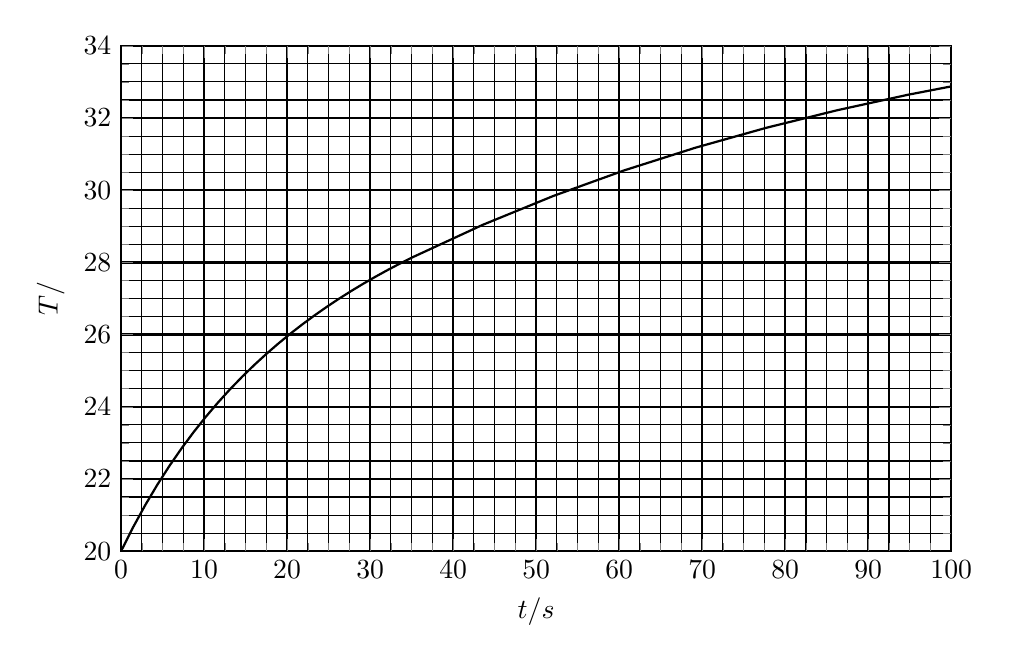
\begin{tikzpicture}
	\begin{axis}[ 
		xlabel={$t/s$},
		width = \textwidth,
		height = 8 cm,
		ylabel={$T/\degreeCelsius$},
		xmin=0, xmax = 100,
		ymin=20, ymax = 34,
		xtick distance = 10,
		ytick distance = 2,
		minor x tick num = 3,
		minor y tick num = 3,
		grid = both,
		minor grid style = {black},
		major grid style = {black, thick},
	] 
	\addplot [domain=0:35, thick]{20 + 2000/(4200*0.03)*(1-1/(1+0.03*x))};
	\addplot [domain=35:240, thick]
	{2000/(4200*0.03)+20+(20+ 2000/(4200*0.03)*(1-1/(1+0.03*35))
		-2000/(4200*0.03)-20)*e^(-0.03*(x-35)/(1+0.03*35))};
	\end{axis}
\end{tikzpicture}
\fi
}

% Ü360
\ylDisplay{Soojustus} % Ülesande nimi
{Ardi Loot} % Autor
{lõppvoor} % Voor
{2018} % Aasta
{G 5} % Ülesande nr.
{7} % Raskustase
{
% Teema: Termodünaamika
\ifStatement
\begin{wrapfigure}[10]{r}{0.5\textwidth}
\vspace{-30pt}
\begin{center}
\includegraphics[width=0.5\textwidth]{2018-v3g-05-kullastunud-aur}
\par\end{center} 
\end{wrapfigure}

Seina soojustus koosneb sisemisest (soojusjuhtivus $k_{1}=\SI{0.07}{W/\left(m\cdot K\right)}$)
ja välimisest kihist (soojusjuhtivus $k_{2}=\SI{0.05}{W/\left(m\cdot K\right)}$).
Nende kihtide vahel on kile, et takistada õhu liikumist läbi seina.
Millist tingimust peab rahuldama sisemise soojustuskihi pakus $L_{1},$
et vältida veeauru kondenseerumist seinas? Seina paksus $L=L_{1}+L_{2}=\SI{30}{cm},$
$L_{2}$ on välimise soojustuskihi paksus, toa temperatuur $T_{1}=\SI{20}{\celsius},$
suhteline õhuniiskus toas $\eta_{1}=\SI{60}{\percent}$ ja välistemperatuur
$T_{2}=\SI{-20}{\celsius}.$ Küllastunud veeauru osarõhu sõltuvus
temperatuurist on toodud joonisel.

\emph{Märkus.} Eeldada, et temperatuur muutub soojustuskihis lineaarselt
kaugusega ja muutuse kiirus on pöördvõrdeline soojusjuhtivusega. 
\fi
}

% Ü361
\ylDisplay{Soojuskiirgus} % Ülesande nimi
{Valter Kiisk} % Autor
{lõppvoor} % Voor
{2006} % Aasta
{G 8} % Ülesande nr.
{8} % Raskustase
{
% Teema: Termodünaamika
\ifStatement
Veeldatud gaaside säilitamisel on tarvis palju tähelepanu pöörata anuma soojusisolatsioonile. Olulise osa soojusvahetusest moodustab soojuskiirgus. Oletagem, et anumal on kahekordsed seinad, mille kiirgusvõimsus pinnaühiku kohta on $\varepsilon \sigma T^4$, kus Stefan-Boltzmanni konstant $\sigma = \SI{5,67e-8}{W/(m^2.K)}$ ja seinte kiirgamisvõime $\varepsilon$ loeme temperatuurist sõltumatuks ja võrdseks \num{0,1}-ga. Vedela lämmastikuga kokkupuutes oleva siseseina temperatuur on $T_s = \SI{77}{K}$, toaõhuga kokkupuutes oleva välisseina temperatuur aga $T_v = \SI{293}{K}$.\\
\osa Leidke soojuskiirgusest tingitud soojusvoog läbi $S = \SI{1}{cm^2}$ suuruse seinapinna.\\
\osa Soojusvoo vähendamiseks asetatakse sise- ja välisseina vahele $N$ õhukest ekraani, mille pind on kaetud samasuguse materjaliga nagu anuma seinad. Mitu korda väheneb selle tulemusena soojusvoog? Põhjendage vastust.

\emph{Märkus.} kehtib Kirchhoffi seadus --- keha neelamisvõime, mis näitab, kui suur osa aine pinnale langevast kiirgusest neeldub, on alati võrdne tema kiirgamisvõimega $\varepsilon$.\\
\fi
}

% Ü362
\ylDisplay{Ahi} % Ülesande nimi
{Stanislav Zavjalov} % Autor
{lõppvoor} % Voor
{2012} % Aasta
{G 7} % Ülesande nr.
{8} % Raskustase
{
% Teema: Termodünaamika
\ifStatement
\begin{wrapfigure}{r}{0.5\textwidth}%
\includegraphics[width=\linewidth]{2012-v3g-07-ahi_graafik}%
\end{wrapfigure}
Väikese metallisulatusahju kütteelemendi võimsus on $P_0 = \SI{50}{W}$.
Toatemperatuuril olev ahi lülitakse sisse ja umbes 12 minuti pärast,
kui selle temperatuur praktiliselt enam ei kasva, pannakse ahju mitu
eelsoojendatud pliitükikest summaarse massiga $m = \SI{265}{g}$. Juuresoleval graafikul (suuremalt
lisalehel) on toodud
ahju temperatuuri sõltuvus ajast. Leidke selle põhjal plii sulamissoojus
$\lambda$.
\fi
}

% Ü363
\ylDisplay{Gaasiküte} % Ülesande nimi
{Ardi Loot} % Autor
{piirkonnavoor} % Voor
{2017} % Aasta
{G 10} % Ülesande nr.
{8} % Raskustase
{
% Teema: Termodünaamika
\ifStatement
Poolsfäärikujulist telki raadiusega $R=\SI{4}{m}$ köetakse
gaasipuhuriga. Seinte soojusjuhtivus on $U=\SI{3}{W/\left(m^{2}\cdot K\right)}$.
Ühe massiühiku gaasi põletamisel eraldub $D=\SI{2.25}{}$ massiühikut vett. Gaasi kütteväärtus on $k=\SI{40}{MJ/kg}$. Välisõhu temperatuur on $T_{0}=\SI{-10}{\celsius}$
ja õhuniiskus $\eta_{0}=\SI{50}{\percent}.$ Kui suur peab olema gaasikütte
võimsus $P$ ja telgi ventileerimise õhuruumala $Q$ ajaühikus, et hoida telgis
temperatuuri $T_{1}=\SI{15}{\celsius}$ ja õhuniiskust $\eta_{1}=\SI{80}{\percent}$?
Kui suur osa küttevõimusest kulub ventileeritava õhu soojendamiseks
ja mitu korda tunnis vahetub telgi õhk?

Õhu tihedus $\rho_{\tilde{o}}=\SI{1.2}{kg/m^{3}}$ ja soojusmahtuvus
$c_{\tilde{o}}=\SI{1.0}{kJ/\left(kg\cdot K\right)}$. Temperatuuril
$T_{0}=\SI{-10}{\celsius}$ mahub õhu ruumalaühikusse maksimaalselt
$G_{0}=\SI{2.3}{g/m^{3}}$ veeauru ning temperatuuril $T_{1}=\SI{15}{\celsius}$
vastavalt $G_{1}=\SI{12.8}{g/m^{3}}.$ Eeldada, et soojakaod läbi
telgi põranda puuduvad.
\fi
}

% Ü364
\ylDisplay{Pooljuht} % Ülesande nimi
{Tundmatu autor} % Autor
{lahtine} % Voor
{2008} % Aasta
{G 10} % Ülesande nr.
{9} % Raskustase
{
% Teema: Termodünaamika
\ifStatement
Graafikul on antud pulgakujulise keraamilisest pooljuhist (nn. PTC takisti) soojendi materjali erijuhtivuse $\sigma$ (\si{1/(\ohm. m)}) sõltuvus temperatuurist $t$(\si{\celsius}). Erijuhtivuseks nimetatakse eritakistuse pöördväärtust. Leida, millise temperatuurini kuumeneb avatud ruumis paiknev sellest materjalist soojendi, kui tema otstele rakendatakse pinge $U_1 = \SI{60}{V}$. Milliseks kujuneb soojendi temperatuur, kui otstele rakendatud pinge on $U_2 = \SI{36}{V}$? On teada, et kui soojendi otstele rakendatakse pinge $U_0 = \SI{30}{V}$, siis soojendi temperatuuriks kujuneb $t_0= \SI{70}{\celsius}$. Välisõhu temperatuur on $t_v = \SI{20}{\celsius}$.

\begin{center}
	\includegraphics[width=\linewidth]{2008-lahg-10-yl}
\end{center}
\fi
}

% Ü365
\ylDisplay{Must kuup} % Ülesande nimi
{Mihkel Pajusalu} % Autor
{lahtine} % Voor
{2014} % Aasta
{G 9} % Ülesande nr.
{9} % Raskustase
{
% Teema: Termodünaamika
\ifStatement
Olgu väga hea soojusjuhtivusega materjalist absoluutselt must kuup paralleelses valgusvihus, mille intensiivsus (võimsus ristlõikepindala kohta) on $I$. Milline on maksimaalne ja minimaalne stabiilne temperatuur $T_\text{max}$ ja $T_\text{min}$, mille kuup saavutab sõltuvalt selle asendist kiirguse leviku suuna suhtes?
\fi
}
\newpage\subsection{\protect\StrSubstitute{Varia}{-}{ }}

% Ü366
\ylDisplay{Kontraktsioon} % Ülesande nimi
{EFO žürii} % Autor
{piirkonnavoor} % Voor
{2018} % Aasta
{G 1} % Ülesande nr.
{1} % Raskustase
{
% Teema: Varia
\ifStatement
Omavahel segatakse $V_v$ liitrit vett ja $V_p$ liitrit piiritust nii, et tekkinud lahuse ruumala $V=\SI{1}{dm^3}$ ning lahuses on massi järgi $p=\SI{44,1}{\percent}$ piiritust. Leidke omavahel segatud vee ja piirituse ruumalad $V_v$ ja $V_p$. Lahuste kokkuvalamisel esineb $\gamma = \SI{6}{\percent}$-line kontraktsioon -- saadud lahuse ruumala on \SI{6}{\percent} väiksem kui vee ja piirituse ruumalade summa. Vee tihedus $\rho_v=\SI{1000}{kg/m^3}$ ning piirituse tihedus $\rho_p=\SI{790}{kg/m^3}$.
\fi
}

% Ü367
\ylDisplay{Tunnel} % Ülesande nimi
{Jaan Kalda} % Autor
{lahtine} % Voor
{2008} % Aasta
{G 3} % Ülesande nr.
{2} % Raskustase
{
% Teema: Varia
\ifStatement
Rong, mis sõidab kiirusega $v = \SI{50}{km/h}$, sisenes hästi pikka tunnelisse. Nii rongi kui tunneli ristlõiget lugeda ruuduks küljepikkusega vastavalt $a = \SI{4}{m}$ ja $b = \SI{6}{m}$. Hinnake, milline on tuule kiirus rongi aknast mõõdetuna.
\fi
}

% Ü368
\ylDisplay{Mobiililaadija} % Ülesande nimi
{Mihkel Kree} % Autor
{piirkonnavoor} % Voor
{2014} % Aasta
{G 4} % Ülesande nr.
{3} % Raskustase
{
% Teema: Varia
\ifStatement
Leiutajad on pakkunud välja toreda seadme matkainimestele oma telefoni laadimiseks. Ühe saapa talla sisse pannakse mehhanism, mis toimib amortisaatorina. Iga kord kui kannale toetutakse, muundatakse mehaaniline töö väikese elektrigeneraatori abil elektrienergiaks. Oletame, et matkaja mass $m=\SI{60}{kg}$ ja ühe sammu ajal vajub tald kokku 
$h=\SI{5}{mm}$ võrra. Antud seadme kasutegur $\eta = \SI{0,2}{}$. Matkaja keskmiseks sammupaari pikkuseks ehk kahe järjestikuse samale kannale astumise vahemaaks võtame $d=\SI{1.5}{m}$. Nüüd tuleb vaid ühendada telefon juhtmega saapa külge ja aku laadimine võib alata.

Arvestage, et tüüpilises nutitelefonis on liitium-polümeeraku, mis töötab pingel $U=\SI{3.7}{V}$. Samuti arvestage, et kui telefon töötaks keskmisel voolutugevusel $I_k=\SI{130}{mA}$, suudaks aku vastu pidada $T=10$ tundi. Arvutage, kui pika maa peab matkaja maha kõndima, et tühi telefoni aku uuesti täis laadida.
\fi
}

% Ü369
\ylDisplay{Laser} % Ülesande nimi
{Valter Kiisk} % Autor
{lõppvoor} % Voor
{2017} % Aasta
{G 3} % Ülesande nr.
{3} % Raskustase
{
% Teema: Varia
\ifStatement
Laserkiir ühtlase diameetriga $d=\SI{1}{mm}$ langeb risti kiilukujulise klaasplaadi esimesele pinnale (pindade vaheline nurk $\varphi=\ang{2}$). Laserkiire koosseisus on monokromaatsed komponendid lainepikkustega $\lambda_1=\SI{355}{nm}$ ja $\lambda_2=\SI{532}{nm}$. Klaasi murdumisnäitajad nendel lainepikkustel on vastavalt $n_1=\num{1.48}$ ja $n_2=\num{1.46}$. Leidke kaugus $l$ klaasplaadist, kus erineva lainepikkusega valguskiired on teineteisest täielikult eraldunud.
\fi
}

% Ü370
\ylDisplay{Kuu} % Ülesande nimi
{Urmo Visk} % Autor
{lõppvoor} % Voor
{2006} % Aasta
{G 5} % Ülesande nr.
{4} % Raskustase
{
% Teema: Varia
\ifStatement
Peegeldusteguriks nimetatakse pinnalt peegeldunud ja pinnale langenud valgusvõimsuste suhet. Säriaeg on ajavahemik, mille vältel langeb fotoaparaadis objektiivi läbinud valgus filmilindile. Päikeselisel sügispäeval on mingi objekti pildistamisel optimaalne säriaeg $t_1 = 1/\SI{8000}{s}$. Sama objekti pildistamisel öösel, kui paistab täiskuu, on optimaalne säriaeg $t_2 = \SI{160}{s}$. Mõlema pildi tegemisel on erinev vaid säriaeg. Hinnake Kuu pinna keskmist peegeldustegurit. Kuu kaugus Maast $R = \SI{384000}{km}$ ja Kuu raadius $r = \SI{1740}{km}$. Kvaliteetse pildi saamiseks peab filmile langev valgusenergia päeval ja öösel olema sama väärtusega ehk fotografeerimisel võib valgustatuse ja optimaalse säriaja lugeda pöördvõrdeliseks.
\fi
}

% Ü371
\ylDisplay{Pindpinevus} % Ülesande nimi
{Koit Timpmann} % Autor
{lahtine} % Voor
{2011} % Aasta
{G 2} % Ülesande nr.
{4} % Raskustase
{
% Teema: Varia
\ifStatement
Klaastoru (raadius $r_1$) asetatakse jämedama klaastoru sisse nii, et nende teljed ühtivad. Seejärel
pannakse mõlemad püsti vette. Leidke, kui suur peaks olema jämedama toru
siseraadius $r_2$, et veetase oleks mõlemas klaastorus sama. Eeldage, et torude
seinad on tühiselt õhukesed.
\fi
}

% Ü372
\ylDisplay{Smurf solaariumis} % Ülesande nimi
{Ants Remm} % Autor
{lahtine} % Voor
{2011} % Aasta
{G 4} % Ülesande nr.
{4} % Raskustase
{
% Teema: Varia
\ifStatement
Smurf veetis solaariumi lampide all ajavahemiku $t = \SI{10}{min} $. Kui suure soojushulga $ Q $
sai Smurf? Joonistel on toodud Smurfile langenud valguse spekter $I$
(intensiivsus lainepikkuse kohta sõltuvalt valguse lainepikkusest, ühik
\SI{e9}{W/m^3}) ning Smurfi	
neeldumisspekter $\varepsilon$ (neelatud ja peale langenud valguse
intensiivsuste suhte
sõltuvus valguse lainepikkusest).
Smurfi efektiivne pindala, kuhu langeb valgus, on $ S = \SI{0,1}{m^2} $.
\begin{center}
\includegraphics[width=0.49\textwidth]{2011-lahg-04-I}
\includegraphics[width=0.49\textwidth]{2011-lahg-04-epsilon}
\end{center}
\fi
}

% Ü373
\ylDisplay{Valgustid} % Ülesande nimi
{Valter Kiisk} % Autor
{piirkonnavoor} % Voor
{2016} % Aasta
{G 7} % Ülesande nr.
{4} % Raskustase
{
% Teema: Varia
\ifStatement
Luminestsentstorust kaugusel $l_1=\SI{15}{cm}$ mõõdeti valgustatuseks $L_1=\SI{8400}{lx}$. Luminestsentstoru võib lugeda hulga pikemaks kaugusest $l_1$. Seevastu üksikust LED-pirnist kaugusel $l_2=\SI{30}{cm}$ mõõdeti valgustatuseks $L_2=\SI{2600}{lx}$. Kontoriruumis kulgevad luminestsentstorud ühe sirge katkematu rivina üle kogu ruumi, paiknedes töötasapinnast kõrgusel $h_1=\SI{1.8}{m}$. Laualambi LED-pirn paikneb kõrgusel $h_2=\SI{40}{cm}$ laua pinnast. Kui suur valgustatus saavutatakse otse valgusti all eraldi üldvalgustuse ja kohtvalgustuse kasutamisel? 

\emph{Märkus.} valgustatus iseloomustab ajaühikus pinnaühikule langevat valgusenergiat.
\fi
}

% Ü374
\ylDisplay{Maja} % Ülesande nimi
{Jaan Kalda} % Autor
{lõppvoor} % Voor
{2008} % Aasta
{G 4} % Ülesande nr.
{5} % Raskustase
{
% Teema: Varia
\ifStatement
Fotol kujutatud maja alumise korruse kõrgus (mõõdetuna esimese korruse akna alumisest servast teise korruse akna alumise servani) on 3 meetrit. Kui kõrgel veepinnast on maja (täpsemalt, tema vundamendi ülemine serv)?

\begin{center}
	\includegraphics[height=\textheight]{2008-v3g-04-yl}
\end{center}
\fi
}

% Ü375
\ylDisplay{Tiik} % Ülesande nimi
{Taavi Pungas} % Autor
{lõppvoor} % Voor
{2013} % Aasta
{G 6} % Ülesande nr.
{5} % Raskustase
{
% Teema: Varia
\ifStatement
\begin{wrapfigure}{r}{0.25\textwidth}%
\includegraphics[width=\linewidth]{2013-v3g-06-lained}%
\end{wrapfigure}
Vaatleme tiiki visatud kivi ümber tekkinud lainetust. Kui kivi kukub vette,
tekib suur hulk erinevate lainepikkustega häiritusi, millest igaüks levib
omaette kiirusega. Nende liitumisel moodustub lainehari, mille liikumist
saame vaadelda. Joonisele (suuremalt lisalehele) on iga kindla ajavahemiku järel kantud selle
laineharja asukoht, mõõtkavaks sirglõik pikkusega~$L$. Laineharja kiirus $v$
sõltub seda parasjagu moodustavate komponentide lainepikkustest $\lambda$ ja vee
sügavusest $h$. Kui kivi vettekukkumisest möödunud aeg $t$ on väike, siis
koosneb lainehari lainepikkustest $\lambda \ll h$ ning laineharja kiirus sõltub
ajast seose $v \approx \frac{gt}{\pi}$ järgi. Kaugemal, kus laineharja
moodustavad häiritused lainepikkusega $\lambda \gg h$, liigub see kiirusega $v
\approx \sqrt{hg}$. Hinnake sügavust $h$ eeldusel, et see oli terve tiigi
ulatuses sama. Vastus andke suhtena~$h/L$.
\fi
}

% Ü376
\ylDisplay{Radoon} % Ülesande nimi
{Mihkel Kree} % Autor
{lõppvoor} % Voor
{2016} % Aasta
{G 5} % Ülesande nr.
{5} % Raskustase
{
% Teema: Varia
\ifStatement
Graptoliitargilliit (tuntud ka diktüoneemakilda nime all) on Põhja-Eestis paljanduv setteline savikivim, mis sisaldab hulgaliselt haruldasi elemente, muu hulgas uraani. Üks tonn kivimit sisaldab \SI{300}{g} uraan-238 isotoopi. Uraani levinuima isotoobi, aatommassiga $238$, poolestusaeg $\tau\idx{U}=\SI{4.5}{}$ miljardit aastat ning selle lagunemisahela vaheetapiks on radioaktiivne element radoon, aatommassiga $222$ ning poolestusajaga $\tau\idx{Rn}=\SI{3.8}{}$ päeva. Radoon on gaas, mida peetakse kopsuvähi tekitajaks, sest sissehingamisel satuvad organismi selle radioaktiivsed laguproduktid. Seetõttu sätestavad vastavad normatiivid, et hoonete ruumiõhus peab radooni aktiivsus olema väiksem kui \SI{200}{Bq/m^3}, kus	Henri Becquereli järgi nimetatud ühik \SI{}{Bq} tähistab üht tuuma lagunemist sekundis.

Matkaja tõi matkalt pahaaimamatult koju kaasa ühe graptoliitargilliidi tükikese massiga $m$ ning paigutas selle magamistuppa kapi peale. Arvestage lihtsustatult, et magamistoas ruumalaga $V=\SI{25}{m^3}$ õhuvahetust ei toimu ning et kogu tekkiv gaasiline radoon väljub kivimist. Leidke kivimitükikese suurim ohutu mass $m$, nii et sellest tingitud radooni aktiivsus jääks veel lubatud normidesse, kui kivimit hoida pikka aega toas. 

\emph{Märkus.} aatommassiühik $u=\SI{1.7e-27}{kg}$.
\fi
}

% Ü377
\ylDisplay{Vihmasadu} % Ülesande nimi
{Jaan Kalda} % Autor
{piirkonnavoor} % Voor
{2012} % Aasta
{G 7} % Ülesande nr.
{7} % Raskustase
{
% Teema: Varia
\ifStatement
Viilkatusega maja katus on peegelsümmeetriline: vertikaalne sümmeetriatasand on
ida-läänesuunaline ning katuse
põhja- ja lõunaküljed on omavahel risti. Mõlemal katusepoolel on vihmaveerenn,
mis kogub katusele langeva vee ning suunab selle tünni.
Sajab vihma ning puhub lõunatuul $u= \SI{6,0}{m/s}$; lõunaküljel paiknev tünn
täitub 2,0 korda kiiremini kui põhjaküljel paiknev tünn; võib
lugeda, et katuse läheduses piiskade langemissuund oluliselt ei muutu.
Milline on piiskade langemise keskmine kiirus (st kiiruse vertikaalkomponent)?
\fi
}

% Ü378
\ylDisplay{Maja} % Ülesande nimi
{Jaan Kalda} % Autor
{lahtine} % Voor
{2008} % Aasta
{G 9} % Ülesande nr.
{8} % Raskustase
{
% Teema: Varia
\ifStatement
Juuresolev joonis on tehtud foto põhjal. Pildistamise hetkel asus fotoaparaat \SI{2}{m} kõrgusel veepinnast. Kasutades antud joonist ja joonlauda määrake nii täpselt kui võimalik vees ujuva poi läbimõõt!

\begin{center}
	\includegraphics[width=0.9\linewidth]{2008-lahg-09-yl}
\end{center}
\fi
}

% Ü379
\ylDisplay{Lööklaine} % Ülesande nimi
{Jaan Kalda} % Autor
{lõppvoor} % Voor
{2015} % Aasta
{G 6} % Ülesande nr.
{8} % Raskustase
{
% Teema: Varia
\ifStatement
Elektrostaatilist lööklainet, mis levib kiirusega $w$ piki $x$-telge, võib kirjeldada elektrilise potentsiaali abil: $U=0$ kui $x<wt$ ning $U=U_0$ kui $x>wt$. Millise kiiruse $v$ omandab lööklaine mõjul algselt paigal seisnud osake massiga $m$ ning laenguga $q$? Vastus andke sõltuvana potentsiaalibarjääri kõrgusest $U_0$. Pöörake tähelepanu asjaolule, et see, kummale poole barjääri osake jääb, sõltub $U_0$ väärtusest. 
\fi
}

% Ü380
\ylDisplay{Õhupalli vari} % Ülesande nimi
{Jaan Kalda} % Autor
{lahtine} % Voor
{2013} % Aasta
{G 10} % Ülesande nr.
{10} % Raskustase
{
% Teema: Varia
\ifStatement
Päikesepaistelisel päeval hõljub õhus kerakujuline läbipaistmatu õhupall, mis
jätab horisontaalsele maapinnale varju, kusjuures poolvarju pikkus on \SI{5,0}{m}
ja laius \SI{2,5}m ning täisvarju pikkus \SI{1,0}{m}. Kui suur on palli
läbimõõt ja kui kõrgel see on maapinnast? Päikese näiv nurkläbimõõt (see on nurk, 
mis moodustub kahe kiire vahel, mis on tõmmatud vaatleja silma juurest 
Päikese diameetri otspunktide juurde) oli sel
päeval $\alpha =0,53^\circ$.
\fi
}
\newpage\subsection{\protect\StrSubstitute{Vedelike mehaanika}{-}{ }}

% Ü381
\ylDisplay{Vedelik} % Ülesande nimi
{Tundmatu autor} % Autor
{lahtine} % Voor
{2005} % Aasta
{G 1} % Ülesande nr.
{1} % Raskustase
{
% Teema: Vedelike mehaanika
\ifStatement
Ühendatud silindrilistesse anumatesse diameetritega $d_1$ ja $d_2$ on valatud vedelik tihedusega $\rho$. Kui palju tõuseb vedeliku tase anumates, kui ühte anumasse pannakse ujuma vedeliku tihedusest väiksema tihedusega keha massiga $m$?
\fi
}

% Ü382
\ylDisplay{Tünn} % Ülesande nimi
{Koit Timpmann} % Autor
{piirkonnavoor} % Voor
{2012} % Aasta
{G 3} % Ülesande nr.
{2} % Raskustase
{
% Teema: Vedelike mehaanika
\ifStatement
Vees ujuva tühja tünni ruumalast on $1/10$ vee sees. Pärast tünni täitmist
tundmatu vedelikuga jääb tünn vee peale ujuma, kuid nüüd on vee sees $9/10$ tünni
ruumalast. Kui suur on tünni valatud vedeliku tihedus? Vee tihedus on
\SI{1000}{kg/m^3}.
\fi
}

% Ü383
\ylDisplay{Auk tünnis} % Ülesande nimi
{Hans Daniel Kaimre} % Autor
{lõppvoor} % Voor
{2018} % Aasta
{G 2} % Ülesande nr.
{3} % Raskustase
{
% Teema: Vedelike mehaanika
\ifStatement
Suure vett täis tünni põhjas on auk, kust voolab vett välja. Graafikul on esitatud väljuva veejoa läbimõõdu sõltuvus kaugusest tünni põhjast $l$. Leidke veetaseme kõrgus tünnis.

\begin{center}
\includegraphics[width = 0.6\linewidth]{2018-v3g-02-juga.pdf}
\end{center}
\fi
}

% Ü384
\ylDisplay{Veetoru} % Ülesande nimi
{Taavi Pungas} % Autor
{lõppvoor} % Voor
{2011} % Aasta
{G 4} % Ülesande nr.
{4} % Raskustase
{
% Teema: Vedelike mehaanika
\ifStatement
% kuidas kirjutada const?
Kaks erineva diameetriga horisontaalset toru on otsapidi
kokku ühendatud nii, et nende teljed ühtivad. Mööda esimest toru voolab vesi
kiirusega $v_1$. Kummagi veetoru külge on ühendatud väike vertikaalne toruke,
vedelikusamba kõrgused neis on vastavalt $h_1$ ja $h_2$ (toru teljest mõõtes). Leidke
horisontaalsete torude diameetrite suhe. Hõõrdumist mitte arvestada. 

\emph{Vihje}. 
Vedeliku horisontaalsel voolamisel kehtib Bernoulli seadus kujul $\frac{\rho v^2}{2}+p=\const$, kus $p$ on hüdrostaatiline rõhk, $\rho$ vedeliku tihedus ning $v$ vedeliku kiirus.
\fi
}

% Ü385
\ylDisplay{Ujuv kuup} % Ülesande nimi
{Koit Timpmann} % Autor
{lõppvoor} % Voor
{2015} % Aasta
{G 3} % Ülesande nr.
{4} % Raskustase
{
% Teema: Vedelike mehaanika
\ifStatement
Õhukeseseinaline hermeetiline kuup ujub vee pinnal. Vee tihedus on $\rho$, kuubi mass koos selles oleva gaasiga $m$ ja selle serva pikkus $a$. Milline on vähim gaasi algrõhk kuubis $p$, mille korral kuup ei upuks, kui selle põhja tekiks auk? Õhurõhk on $p_0$, raskuskiirendus on $g$.
\fi
}

% Ü386
\ylDisplay{Pump} % Ülesande nimi
{Ardi Loot} % Autor
{piirkonnavoor} % Voor
{2018} % Aasta
{G 4} % Ülesande nr.
{4} % Raskustase
{
% Teema: Vedelike mehaanika
\ifStatement
Kaevust sügavusega $h=\SI{5.0}{m}$ tahetakse pumbata vett. Pump asub
maapinnal ning selle veevõtutoru (täidetud veega) on siseläbimõõduga
$d=\SI{16}{mm}$ ja pikkusega, mis on võrdne kaevu sügavusega.\\
\osa Kui suur peab olema pumba võimsus $P$, et pumbata vett vooluhulgaga
$q=\SI{30}{l/min}$? Pumba kasutegur on $\eta=\SI{25}{\percent}$.\\
\osa Missugune on maksimaalne kaevu sügavus $h_{m}$, mille korral on
võimalik sellist tüüpi pumbaga kaevust vett pumbata?

Arvestada, et torus olevale veesambale mõjub lisaks teistele jõududele
ka hõõrdejõud, mis põhjustab rõhu vähenemist toru pikkuse $l$ kohta $\Delta p=c_{h}q^{2}l/d^{5},$
kus $c_{h}=\SI{40}{Pa\cdot s^{2}/m^{2}}.$ Vee tihedus $\rho=\SI{1000}{kg/m^{3}}$,
raskuskiirendus $g=\SI{9.8}{m/s^{2}}$ ja õhurõhk $p_{0}=\SI{100}{kPa}.$
\fi
}

% Ü387
\ylDisplay{Veekahur} % Ülesande nimi
{Oleg Košik} % Autor
{piirkonnavoor} % Voor
{2005} % Aasta
{G 7} % Ülesande nr.
{5} % Raskustase
{
% Teema: Vedelike mehaanika
\ifStatement
Veekahur laseb veejoaga, mille ristlõikepindala on $S = \SI{8}{cm^2}$ ning võimsus $N = \SI{6000}{W}$. Millise jõuga tabab veejuga märki, kui kahur ja märk asuvad samal kõrgusel? Vee tihedus on $\rho = \SI{1000}{kg/m^3}$, õhutakistust mitte arvestada. Märklaua ja veekahuri vahemaa on väike, st veejoa kõverdumisega raskusjõu toimel võib mitte arvestada.
\fi
}

% Ü388
\ylDisplay{Veetünn} % Ülesande nimi
{Mihkel Kree} % Autor
{lõppvoor} % Voor
{2005} % Aasta
{G 5} % Ülesande nr.
{5} % Raskustase
{
% Teema: Vedelike mehaanika
\ifStatement
Silindriline veetünn, milles hoitakse muutumatut veetaset kõrgusega $h$, on tõstetud horisontaalsele platvormile, mille kõrgus maapinnast on $H$ (vt joonist). Tünni seina kõrgusele $a$ selle põhjast puuritakse auk. Väljuv veejuga puudutab maapinda kaugusel $L$ platvormi jalamist. Graafikul on kujutatud kauguse $L$ sõltuvus augu kõrgusest $x = a/h$. Määrake tünni kõrgus $h$ ning aluse kõrgus $H$ eeldusel, et $h > H$.

\begin{center}
	\includegraphics[width=\linewidth]{2005-v3g-05-yl}
\end{center}
\fi
}

% Ü389
\ylDisplay{Veejuga} % Ülesande nimi
{Siim Ainsaar} % Autor
{piirkonnavoor} % Voor
{2006} % Aasta
{G 9} % Ülesande nr.
{5} % Raskustase
{
% Teema: Vedelike mehaanika
\ifStatement
Vesi voolab kraanist vertikaalselt alla purki. Nagu teada, ei ole kraanist voolav veejuga silindriline. Joa raadius kraani otsa juures on $r_0 = \SI{5}{mm}$, sellest kaugusel $h = \SI{130}{mm}$ allpool aga $r_1 = \SI{3}{mm}$. Leidke aeg $t$, mis kulub purgi täitmiseks, kui raskuskiirendus on $g = \SI{9,8}{m/s}$. Purgi ruumala $V = \SI{1}{liiter}$. Pindpinevusest tingitud efekte pole vaja arvestada. Eeldada, et voolamiskiirus on iga ristlõike piires ühesugune ning keeriseid ei ole. 
\fi
}

% Ü390
\ylDisplay{Veepüstol} % Ülesande nimi
{Valter Kiisk} % Autor
{lõppvoor} % Voor
{2006} % Aasta
{G 4} % Ülesande nr.
{5} % Raskustase
{
% Teema: Vedelike mehaanika
\ifStatement
Veepüstoliga (vt joonist) tekitatakse veejuga, surudes vett läbi kitsa silindrilise suudme, mille sisediameeter on $d_2 = \SI{1}{mm}$. Päästik on ühendatud kolviga, mis saab tihedalt liikuda silindrilises torus diameetriga $d_1 = \SI{1}{cm}$. Oletagem, et sõrmed suruvad päästikule jõuga $F = \SI{20}{N}$ (jõu rakenduspunkt ja suund on näidatud joonisel). Kui suure kiirusega väljub veejuga püstolist? Vee liikumise võib lugeda laminaarseks, vee viskoossust ja püstoli liikuvatele osadele mõjuvaid hõõrdejõude võib ignoreerida. Vee tihedus on $\rho = \SI{1000}{kg/m^3}$

\begin{center}
	\includegraphics[width=0.6\linewidth]{2006-v3g-04-yl}
\end{center}
\fi
}

% Ü391
\ylDisplay{U-toru} % Ülesande nimi
{Tundmatu autor} % Autor
{lahtine} % Voor
{2009} % Aasta
{G 6} % Ülesande nr.
{5} % Raskustase
{
% Teema: Vedelike mehaanika
\ifStatement
\begin{wrapfigure}[9]{r}{0.4\textwidth}
	\begin{center}
		\vspace{-15pt}
		\includegraphics[width=\linewidth]{2009-lahg-06-yl}
	\end{center}
\end{wrapfigure}
Teatud torustikes võib vedeliku surve olla nii tugev, et torud võivad märgatavalt deformeeruda. Vaatleme sellist deformatsiooni U-kujulises torus (vt joonist): kaks sirget pikkusega $l$ terastoru, mille välisraadius on $\sqrt 2$ korda suurem siseraadiusest, on ühendatud sama sisemise raadiusega mittedeformeeruvast materjalist kaarekujulise toruga. Selles U-torus voolab vedelik tihedusega $\rho$ ja konstantse voolukiirusega $v$. Vedeliku hüdrostaatiline rõhk lugeda võrdseks välisrõhuga. U-toru otsad on pinnal jäigalt kinnitatud. Eeldades, et õõnsa terastoru deformatsiooni jaoks toimib Hooke’i seadus, kusjuures jäikustegur avaldub kujul $k = ES/l$ ($E$ on terase nn Young’i konstant, $S$ on toru ristlõike pindala ja $l$ on deformeerimata toru pikkus), leidke toru pikenemine.
\fi
}

% Ü392
\ylDisplay{Veeklaas} % Ülesande nimi
{Siim Ainsaar} % Autor
{piirkonnavoor} % Voor
{2013} % Aasta
{G 7} % Ülesande nr.
{5} % Raskustase
{
% Teema: Vedelike mehaanika
\ifStatement
Silindrilisse klaasi, mille kõrgus on $H$ ja põhja raadius $r$, valati
vett kõrguseni $h$. Klaas kaeti paberilehega ja keerati
tagurpidi; paberi ja
klaasi vahelt voolas välja veekogus ruumalaga $V$. Kui paberit enam kinni ei
hoitud, jäi see sellegipoolest klaasi külge, ülejäänud vesi püsis klaasis.
Kui suur oli maksimaalselt paberi mass $m$? Õhurõhk oli $p_0$,
raskuskiirendus $g$ ning vee tihedus $\varrho$.
Kasutati kriitpaberit, mis vett ei imanud. Paberist lahtilaskmise hetkel olid 
õhu ja vee temperatuurid võrdsed.
\fi
}

% Ü393
\ylDisplay{Klots vedelikes} % Ülesande nimi
{Erkki Tempel} % Autor
{lahtine} % Voor
{2014} % Aasta
{G 6} % Ülesande nr.
{5} % Raskustase
{
% Teema: Vedelike mehaanika
\ifStatement
Silindrilises anumas põhja pindalaga $S$ on kaks mittesegunevat vedelikku tihedustega $\rho_1$ ja $\rho_2$. Anumasse asetatakse kuubikujuline klots ruumalaga $V$ ning tihedusega $\rho_k$ ($\rho_1>\rho_k>\rho_2$). Klots on täielikult vedelike sees ega puuduta anuma põhja.\\
\osa Kui suur osa klotsist asub alumises vedelikus?\\
\osa Kui palju muutub kahe vedeliku eralduspinna kõrgus pärast klotsi asetamist anumasse?
\fi
}

% Ü394
\ylDisplay{Kuup veega} % Ülesande nimi
{Jonatan Kalmus} % Autor
{piirkonnavoor} % Voor
{2018} % Aasta
{G 7} % Ülesande nr.
{5} % Raskustase
{
% Teema: Vedelike mehaanika
\ifStatement
Leidke veekoguse mass, mis tuleb valada kuupi, et see oleks võimalikult stabiilne, ehk süsteemi massikese oleks võimalikult madalal. Kuubi külje pikkus on $a$, mass $M$, vee tihedus $\rho$. Kuubi seina paksusega mitte arvestada. Kuup on täielikult sümmeetriline ehk sellel on olemas kõik 6 identset tahku.
\fi
}

% Ü395
\ylDisplay{Allveelaev} % Ülesande nimi
{Mihkel Heidelberg} % Autor
{lahtine} % Voor
{2012} % Aasta
{G 5} % Ülesanne nr.
{6} % Raskustase
{
% Teema: Vedelike mehaanika
\ifStatement
\begin{wrapfigure}{r}{0.51\linewidth}%
\includegraphics[width=\linewidth]{2012-lahg-05-allveelaev_g}%
\end{wrapfigure}
Salaagent Bond põgeneb allveelaevalt selle torni kaudu. Tornis on algselt
rõhk sama mis õhurõhk vee peal: $p_0 = \SI{100}{kPa}$. Pärast torni ja ülejäänud
allveelaeva eraldava luugi sulgemist teeb ta seina sisse augu (vaata joonist), misjärel
täitub torn osaliselt veega. Seejärel avab Bond torni laeluugi ja ujub
koos vabaneva õhuga pinnale.\\
\osa Kui paks on õhukiht, mis jääb torni enne torni
laeluugi avamist ja pärast vee sissevoolamise lõppemist?\\
\osa Kui suur ja mis suunas (üles või alla) on õhu ja vee poolt laeluugile avaldatav summaarne jõud enne
avamist, kui veetase torni sees on jäänud paigale?
\par
Luugi pindala $S =
\SI{0,50}{m^2}$, veetase luugi kohal $h=\SI{25}{m}$, torni kõrgus 
$s=\SI{2,0}{m}$. Vee tihedus $\rho = \SI{1000}{kg/m^3}$, raskuskiirendus $g =
\SI{9,8}{m/s^2}$.
\fi
}

% Ü396
\ylDisplay{Ookean} % Ülesande nimi
{Tundmatu autor} % Autor
{lahtine} % Voor
{2005} % Aasta
{G 8} % Ülesande nr.
{7} % Raskustase
{
% Teema: Vedelike mehaanika
\ifStatement
Vee kokkusurutavuse tegur $\beta = \SI{5e-5}{atm^{-1}}$.\\
\osa Hinnake ookeani keskmise sügavuse muutumist juhul, kui vesi oleks täielikult kokkusurumatu. Ookeani keskmine sügavus $h \approx \SI{3800}{m}$.\\
\osa Hinnake vee tiheduste vahet $\Delta \rho$ veepinnalähedasel veel ja veel ookeani süvendi põhjas sügavusel $H = \SI{10}{km}$. 

\emph{Märkus}. kokkusurutavuse tegur $\beta$ näitab keha ühikulise ruumala vähenemist rõhu suurenemisel ühe ühiku võrra. Atmosfäär on rõhu mõõtmise ühik, mis võrdub atmosfääri normaalrõhuga merepinna kõrgusel: \SI{1}{atm} = \SI{101325}{Pa}.
\fi
}

% Ü397
\ylDisplay{Kauss} % Ülesande nimi
{Taavi Pungas} % Autor
{lahtine} % Voor
{2013} % Aasta
{G 7} % Ülesande nr.
{7} % Raskustase
{
% Teema: Vedelike mehaanika
\ifStatement
Silindrikujuline metallkauss massiga $M=\SI{1}{kg}$ ja ruumalaga
$V_1=\SI{3}{dm^3}$ ujub vannis. Mari teeb eksperimenti ja valab ühtlaselt
$t=\SI{1}{s}$ jooksul kõrguselt $h=\SI{1,5}{m}$ kaussi kannutäie vett ruumalaga
$V_2=\SI{1,5}{dm^3}$. Ennustage eksperimendi tulemust: kas kauss läheb põhja või
ei? Põhjendage oma ennustust arvutustega. Vee tihedus $\rho=\SI{1000}{kg/m^3}$.
\fi
}

% Ü398
\ylDisplay{Veejoad} % Ülesande nimi
{Mihkel Kree} % Autor
{lahtine} % Voor
{2015} % Aasta
{G 7} % Ülesande nr.
{7} % Raskustase
{
% Teema: Vedelike mehaanika
\ifStatement
\begin{wrapfigure}{r}{0.2\textwidth}%
\vspace{-15pt}
\includegraphics[width=\linewidth]{2015-lahg-07-veejoadJoon}%
\end{wrapfigure}
Vertikaalse silindrilise anuma seina sisse on paljudele erinevatele kõrgustele tehtud pisikesed augud, millest voolab välja vett. Anumasse valatakse aeglaselt vett juurde nii, et veetase anumas püsib muutumatuna kõrgusel $H$. Leidke, millisesse ruumipiirkonda saab anumast väljuv vesi jõuda ehk avaldage veejugade mähispinna võrrand $xy$-teljestikus. Eeldage, et erinevad veejoad üksteist ei mõjuta.
\fi
}

% Ü399
\ylDisplay{U-toru} % Ülesande nimi
{Erkki Tempel} % Autor
{piirkonnavoor} % Voor
{2016} % Aasta
{G 9} % Ülesande nr.
{7} % Raskustase
{
% Teema: Vedelike mehaanika
\ifStatement
U-torusse ühtlase ristlõikepindalaga S on valatud vesi tihedusega $\rho_v$, nii et üle poole U-torust on veega täidetud ja kummagi täitmata osa pikkus on $h$. U-toru üks ots suletakse hermeetiliselt ning teise torusse valatakse aeglaselt õli kuni U-toru ülemise servani. Kui suur oli õli tihedus $\rho_{\text{õ}}$, kui on teada, et lisatud õlisamba kõrgus oli $l$? Atmosfäärirõhk on $p_0$.
\fi
}

% Ü400
\ylDisplay{V-toru} % Ülesande nimi
{Mihkel Kree} % Autor
{lõppvoor} % Voor
{2008} % Aasta
{G 8} % Ülesande nr.
{8} % Raskustase
{
% Teema: Vedelike mehaanika
\ifStatement
Toomas mängib läbipaistvast aiavoolikust tehtud U-toruga. Et seekordne U-toru polegi klaasist, painutab ta üht poolt nurga $\alpha$ ning teist $\beta$ võrra (vt joonist). Kas vedelikutaseme võnkesagedus on nüüd suurem või väiksem, mitu korda? 

\emph{Märkus}. Vertikaalses U-torus on vedelikutaseme võnkumise sagedus $f = \frac{1}{2\pi} \sqrt{\frac{2S\rho g}{m}}$, kus $S$ on toru ristlõikepindala, $\rho$ vedeliku tihedus ning $m$ torus oleva vedeliku mass.

\begin{center}
	\includegraphics[width=0.5\linewidth]{2008-v3g-08-yl}
\end{center}
\fi
}
\newpage\normalsize\section{Vihjed}
        \ToggleHint
        
% V1
\ylDisplay{Kivi} % Ülesande nimi
{Aigar Vaigu} % Autor
{lõppvoor} % Voor
{2005} % Aasta
{G 1} % Ülesande nr.
{1} % Raskustase
{
% Teema: Dünaamika

\ifHint
Maksimaalse viivituse korral on palli kiirus vaevu kivi omast suurem. Selles on võimalik veenduda liikudes vabalt langevasse taustsüsteemi. Seal liiguvad vabalt langevad kehad konstantse kiirusega ning selleks, et pall ja kivi kokku põrkaksid, peaks nende suhteline kiirus olema negatiivne.
\fi
}

% V2
\ylDisplay{Pallid} % Ülesande nimi
{Tundmatu autor} % Autor
{lahtine} % Voor
{2007} % Aasta
{G 1} % Ülesande nr.
{1} % Raskustase
{
% Teema: Dünaamika

\ifHint
Kuna pallid on samasuguse massiga ja tegu on elastse kokkupõrkega, vahetavad pallid oma kiirusvektorid. Seega võime sama hästi öelda, et pallid lähevad üksteisest vabalt läbi.
\fi
}

% V3
\ylDisplay{Hobune} % Ülesande nimi
{Valter Kiisk} % Autor
{piirkonnavoor} % Voor
{2007} % Aasta
{G 1} % Ülesande nr.
{1} % Raskustase
{
% Teema: Dünaamika

\ifHint
Langemise aeg on avaldatav valemi $s = \frac{at^2}{2}$ kaudu.
\fi
}

% V4
\ylDisplay{Eiffeli torn} % Ülesande nimi
{Aigar Vaigu} % Autor
{piirkonnavoor} % Voor
{2010} % Aasta
{G 1} % Ülesande nr.
{1} % Raskustase
{
% Teema: Dünaamika

\ifHint
Kukkumise käigus kiirenevad mõlemad kuulid sama kiirusega. Seega on nende suhteline kiirus muutumatu.
\fi
}

% V5
\ylDisplay{Kokkupõrge} % Ülesande nimi
{Andreas Valdmann} % Autor
{piirkonnavoor} % Voor
{2011} % Aasta
{G 1} % Ülesande nr.
{1} % Raskustase
{
% Teema: Dünaamika

\ifHint
\osa Energia jäävuse seaduse kohaselt kulub purustuse tekitamiseks esialgse ja pärastise kineetiliste energiate vahe.\\
\osa Taustsüsteemide vahetamine lihtsustab olukorda oluliselt.
\fi
}

% V6
\ylDisplay{Lendav pudel} % Ülesande nimi
{Erkki Tempel} % Autor
{piirkonnavoor} % Voor
{2014} % Aasta
{G 1} % Ülesande nr.
{1} % Raskustase
{
% Teema: Dünaamika

\ifHint
Nii pudelile kui veele mõjuvad täpselt samad jõud ning neid visatakse sama algkiirusega.
\fi
}

% V7
\ylDisplay{Potsataja ja pähklid} % Ülesande nimi
{Erkki Tempel} % Autor
{piirkonnavoor} % Voor
{2014} % Aasta
{G 2} % Ülesande nr.
{1} % Raskustase
{
% Teema: Dünaamika

\ifHint
Antud olukorda on mugavam vaadelda rongiga kaasa liikuvas taustsüsteemis.
\fi
}

% V8
\ylDisplay{Kurv} % Ülesande nimi
{Mihkel Rähn} % Autor
{lahtine} % Voor
{2016} % Aasta
{G 2} % Ülesande nr.
{1} % Raskustase
{
% Teema: Dünaamika

\ifHint
Autos istujad ei tunne külgsuunalist jõudu siis, kui summaarne jõud on tee pinnaga risti.
\fi
}

% V9
\ylDisplay{Tõus} % Ülesande nimi
{Tundmatu autor} % Autor
{lahtine} % Voor
{2005} % Aasta
{G 2} % Ülesande nr.
{2} % Raskustase
{
% Teema: Dünaamika

\ifHint
Mäe tippu jõudmiseks peab esialgne kineetiline energia olema suurem kui hõõrdejõu ja raskusjõu ületamiseks vajalik töö.
\fi
}

% V10
\ylDisplay{Keha} % Ülesande nimi
{Tundmatu autor} % Autor
{lahtine} % Voor
{2006} % Aasta
{G 3} % Ülesande nr.
{2} % Raskustase
{
% Teema: Dünaamika

\ifHint
Ülesse visatud keha vertikaalne koordinaat avaldub vastavalt liikumisvõrrandile kui $h = v_0t - \frac{gt^2}{2}$. Kuna tegu on ruutvõrrandiga, leidub fikseeritud $h$ jaoks kaks ajahetke, mil keha sellel kõrgusel on.
\fi
}

% V11
\ylDisplay{Mootorratas} % Ülesande nimi
{Tundmatu autor} % Autor
{lahtine} % Voor
{2007} % Aasta
{G 5} % Ülesande nr.
{2} % Raskustase
{
% Teema: Dünaamika

\ifHint
Tegu on suhteliselt sirgjoonelise ballistilise probleemiga. Mootorratturi kiirus peab olema selline, et mootorratturi paraboolne trajektoor läbiks kraavi vastasnurka.
\fi
}

% V12
\ylDisplay{Kelk} % Ülesande nimi
{Tundmatu autor} % Autor
{lahtine} % Voor
{2008} % Aasta
{G 2} % Ülesande nr.
{2} % Raskustase
{
% Teema: Dünaamika

\ifHint
Kehtib energia jäävuse seadus. Koguenergiate vahe alg- ja lõppseisu vahel kulus hõõrdejõu ületamiseks vajalikuks tööks mõlemal mäenõlval.
\fi
}

% V13
\ylDisplay{Hantel} % Ülesande nimi
{Mihkel Kree} % Autor
{lõppvoor} % Voor
{2008} % Aasta
{G 1} % Ülesande nr.
{2} % Raskustase
{
% Teema: Dünaamika

\ifHint
Massikeskme kulgliikumise energia muundub maksimaalsele kõrgusele jõudes täielikult potentsiaalseks energiaks.
\fi
}

% V14
\ylDisplay{Ping-pong} % Ülesande nimi
{Siim Ainsaar} % Autor
{lõppvoor} % Voor
{2008} % Aasta
{G 2} % Ülesande nr.
{2} % Raskustase
{
% Teema: Dünaamika

\ifHint
Palli koguenergia vastab geomeetrilisele jadale, sest iga järgmise põrke energia on eelnevast $k$ korda väiksem. Saame sarnase jada, kui avaldame kahe järjestikuse põrke vahelise aja summaarse energia kaudu.
\fi
}

% V15
\ylDisplay{Mürsk} % Ülesande nimi
{Mihkel Kree} % Autor
{piirkonnavoor} % Voor
{2009} % Aasta
{G 2} % Ülesande nr.
{2} % Raskustase
{
% Teema: Dünaamika

\ifHint
Vedrumehanismi vallandumisel muutub osa vedrudesse salvestatud potentsiaalsest energiast kineetiliseks energiaks --- seega kineetilise energia jäävus ei kehti. See-eest kehtib impulsi jäävuse seadus, sest lagunemise käigus ei mõju mürsule väliseid jõude (eeldusel, et mürsk laguneb hetkeliselt).
\fi
}

% V16
\ylDisplay{Kerad} % Ülesande nimi
{Valter Kiisk} % Autor
{lahtine} % Voor
{2010} % Aasta
{G 1} % Ülesande nr.
{2} % Raskustase
{
% Teema: Dünaamika

\ifHint
Õõnes ja homogeenne kera erinevad nende intertsimomentide poolest. Vedelikku sisaldaval keral toimub sees paratamatult hõõrdumine ning seega energia kadu vedeliku erinevate kihtide vahel.
\fi
}

% V17
\ylDisplay{Sild} % Ülesande nimi
{Valter Kiisk} % Autor
{lõppvoor} % Voor
{2010} % Aasta
{G 1} % Ülesande nr.
{2} % Raskustase
{
% Teema: Dünaamika

\ifHint
Silla kõverusraadius on leitav Pythagorase teoreemist. Autole mõjub silla peal kaks jõudu: raskusjõud ja rõhumisjõud. Antud jõudude resultant annab kesktõmbekiirenduse.
\fi
}

% V18
\ylDisplay{Varras} % Ülesande nimi
{Stanislav Zavjalov} % Autor
{lõppvoor} % Voor
{2011} % Aasta
{G 2} % Ülesande nr.
{2} % Raskustase
{
% Teema: Dünaamika

\ifHint
Ülesanne näeb keerulisem välja kui see tegelikult on. Olukorda lihtsustab oluliselt asjaolu, et varras on tühiselt kerge ja libisemised hõõrdevabad.
\fi
}

% V19
\ylDisplay{Kadunud rahakott} % Ülesande nimi
{Eero Vaher} % Autor
{lahtine} % Voor
{2012} % Aasta
{G 2} % Ülesanne nr.
{2} % Raskustase
{
% Teema: Dünaamika

\ifHint
Hoovõturaja alumises otsas on rahakott omandanud teatud horisontaalse kiiruse. Edasi hakkab rahakott liikuma mööda paraboolset trajektoori, kuni see taas vastu mäe nõlva kukub.
\fi
}

% V20
\ylDisplay{Kivi} % Ülesande nimi
{Taavi Pungas} % Autor
{lahtine} % Voor
{2013} % Aasta
{G 1} % Ülesande nr.
{2} % Raskustase
{
% Teema: Dünaamika

\ifHint
Tikk hakkab poolkera pealt maha libisema siis, kui raskusjõu pinnaga paralleelne komponent ületab hõõrdejõu.
\fi
}

% V21
\ylDisplay{Kelgutaja} % Ülesande nimi
{Taavi Pungas} % Autor
{piirkonnavoor} % Voor
{2013} % Aasta
{G 4} % Ülesande nr.
{2} % Raskustase
{
% Teema: Dünaamika

\ifHint
Fikseeritud $h$ ja $t$ puhul on nõlva kalle vähim siis, kui hõõrdejõud puudub.
\fi
}

% V22
\ylDisplay{Pall} % Ülesande nimi
{Taivo Pungas} % Autor
{lõppvoor} % Voor
{2013} % Aasta
{G 2} % Ülesande nr.
{2} % Raskustase
{
% Teema: Dünaamika

\ifHint
Palli lennu kõrgus sõltub vastavale kõrgusele jõudmise aja ruudust.
\fi
}

% V23
\ylDisplay{Kaubarong} % Ülesande nimi
{Mihkel Rähn} % Autor
{lahtine} % Voor
{2014} % Aasta
{G 1} % Ülesande nr.
{2} % Raskustase
{
% Teema: Dünaamika

\ifHint
\osa Horisontaalsel teel peab kaubarong ületama takistava hõõrdejõu.\\
\osa Lisaks hõõrdejõule peab rong nüüd ületama ka raskusjõu.
\fi
}

% V24
\ylDisplay{Vaakumkahur} % Ülesande nimi
{Andreas Valdmann} % Autor
{lahtine} % Voor
{2014} % Aasta
{G 2} % Ülesande nr.
{2} % Raskustase
{
% Teema: Dünaamika

\ifHint
Pall jaotab kahuritoru kaheks kambriks. Pärast vasakpoolse membraani purustamist hakkab vasakpoolses kambris olev gaas palli paremale poole suruma.
\fi
}

% V25
\ylDisplay{Mängukahur} % Ülesande nimi
{EFO žürii} % Autor
{lahtine} % Voor
{2016} % Aasta
{G 1} % Ülesande nr.
{2} % Raskustase
{
% Teema: Dünaamika

\ifHint
Kuna pall maandub kaldpinnale risti, siis liigub pall sellel hetkel nurgaga $\alpha$ vertikaali suhtes. Seega tulistatakse pall kahurist välja samuti nurga $\alpha$ all vertikaali suhtes ning pall põrkab kaldpinnalt tagasi sama nurga all.
\fi
}

% V26
\ylDisplay{Köievedu} % Ülesande nimi
{Oleg Košik} % Autor
{piirkonnavoor} % Voor
{2016} % Aasta
{G 2} % Ülesande nr.
{2} % Raskustase
{
% Teema: Dünaamika

\ifHint
Vastavalt Newtoni III seadusele on nööri tõmme mõlema mehe jaoks sama suur, kuid vastupidises suunas. Lisaks nööri tõmbele mõjub kummalegi mehele vastassuunas hõõrdejõud.
\fi
}

% V27
\ylDisplay{Vastlaliug} % Ülesande nimi
{Moorits Mihkel Muru} % Autor
{lõppvoor} % Voor
{2017} % Aasta
{G 1} % Ülesande nr.
{2} % Raskustase
{
% Teema: Dünaamika

\ifHint
Hõõrdejõu tõttu kulutatud energia sõltub läbitud teepikkusest ja selle kaldest, potentsiaalse energia vahe sõltub kõrguse muudust.
\fi
}

% V28
\ylDisplay{Karatist} % Ülesande nimi
{Tundmatu autor} % Autor
{lahtine} % Voor
{2007} % Aasta
{G 6} % Ülesande nr.
{3} % Raskustase
{
% Teema: Dünaamika

\ifHint
Löögi hetkel kehtib impulsi jäävus, aga energia ei säili. See-eest säilib mehaaniline energia pärast põrget toimuval liikumisel.
\fi
}

% V29
\ylDisplay{Veenus} % Ülesande nimi
{Mihkel Kree} % Autor
{lõppvoor} % Voor
{2007} % Aasta
{G 2} % Ülesande nr.
{3} % Raskustase
{
% Teema: Dünaamika

\ifHint
\osa Maksimaalse eemaldumise korral moodustub Maast, Veenusest ja Päikesest täisnurkne kolmnurk, mille täisnurga tipp on Veenus.\\
\osa Maa ja Veenuse suhtelise nurga (Päikeselt vaadatuna) muutus on avaldatav planeetide nurkkiiruste vahe kaudu.
\fi
}

% V30
\ylDisplay{Auto} % Ülesande nimi
{Mihkel Heidelberg} % Autor
{piirkonnavoor} % Voor
{2009} % Aasta
{G 5} % Ülesande nr.
{3} % Raskustase
{
% Teema: Dünaamika

\ifHint
Nii auto liikumisse kui ka mootori tööse minevad võimsused on avaldatavad rataste ja maa vahelise hõõrdejõu kaudu.
\fi
}

% V31
\ylDisplay{Vedru} % Ülesande nimi
{Aigar Vaigu} % Autor
{piirkonnavoor} % Voor
{2010} % Aasta
{G 4} % Ülesande nr.
{3} % Raskustase
{
% Teema: Dünaamika

\ifHint
Tellise eemaldumise hetkel on vedru alumine ots paigal, aga ülemine ots liigub tellisega sama kiirusega ülesse.
\fi
}

% V32
\ylDisplay{Pendel} % Ülesande nimi
{Taavi Pungas} % Autor
{piirkonnavoor} % Voor
{2011} % Aasta
{G 7} % Ülesande nr.
{3} % Raskustase
{
% Teema: Dünaamika

\ifHint
Pendli perioodi leidmiseks on võimalik teha esialgne jäme hinnang, mis põhineb järjestikustel mõõtmistel. Täpsema hinnangu jaoks võib kasutada esialgset jämedat hinnangut ja pikemat ajavahemikku, et määrata täpselt mitu võnget antud ajavahemiku sisse mahub.
\fi
}

% V33
\ylDisplay{Alpinist} % Ülesande nimi
{Kaur Aare Saar} % Autor
{lahtine} % Voor
{2013} % Aasta
{G 3} % Ülesande nr.
{3} % Raskustase
{
% Teema: Dünaamika

\ifHint
Jõudes kukkumise madalaimasse punkti, on alpinisti potentsiaalne energia läinud üle vedru potentsiaalseks energiaks. Pannes vastava seose kirja, on võimalik leida nööri pikenemise $x$.
\fi
}

% V34
\ylDisplay{Langevarjuhüpe} % Ülesande nimi
{Taavi Pungas} % Autor
{piirkonnavoor} % Voor
{2014} % Aasta
{G 5} % Ülesande nr.
{3} % Raskustase
{
% Teema: Dünaamika

\ifHint
Nii Jukule kui ka Juhanile mõjub sama koefitsiendiga õhu hõõrdejõud, mis on raskusjõu poolt täielikult tasakaalustatud.
\fi
}

% V35
\ylDisplay{Kelk} % Ülesande nimi
{Joonas Kalda} % Autor
{piirkonnavoor} % Voor
{2016} % Aasta
{G 4} % Ülesande nr.
{3} % Raskustase
{
% Teema: Dünaamika

\ifHint
Piirjuhul läheb kogu Juku potentsiaalne energia hõõrdejõu poolt eraldatud soojusenergiaks.
\fi
}

% V36
\ylDisplay{Pidurdus} % Ülesande nimi
{Eero Vaher} % Autor
{lõppvoor} % Voor
{2016} % Aasta
{G 2} % Ülesande nr.
{3} % Raskustase
{
% Teema: Dünaamika

\ifHint
Auto kineetiline energia kulub pidurdusjõu ületamiseks ning potentsiaalse energia muuduks.
\fi
}

% V37
\ylDisplay{Kahurikuul} % Ülesande nimi
{Hans Daniel Kaimre} % Autor
{lõppvoor} % Voor
{2016} % Aasta
{G 3} % Ülesande nr.
{3} % Raskustase
{
% Teema: Dünaamika

\ifHint
Selleks, et leida tegelikku kuuli kõrgust Maa pinnast, võib rakendada energia jäävuse seadust kuuli laskmise hetkel ja trajektoori kõrgeimas punktis.
\fi
}

% V38
\ylDisplay{Pendel} % Ülesande nimi
{Andreas Valdmann} % Autor
{piirkonnavoor} % Voor
{2017} % Aasta
{G 3} % Ülesande nr.
{3} % Raskustase
{
% Teema: Dünaamika

\ifHint
Koormisele mõjuvad kolm jõudu: niidi pinge, raskuskiirendus ja kesktõmbekiirendus. Lisaks peab resultantjõud olema risti nööriga, sest vastasel juhul peaks koormise kiirenemisel nöör venima või lühenema.
\fi
}

% V39
\ylDisplay{Mäenõlv} % Ülesande nimi
{Jonatan Kalmus} % Autor
{lõppvoor} % Voor
{2017} % Aasta
{G 2} % Ülesande nr.
{3} % Raskustase
{
% Teema: Dünaamika

\ifHint
Poole pedaalipöörde jooksul peab ratturi poolt tehtav töö kompenseerima ratta massikeskme tõusmisest kaasneva potentsiaalse energia muudu.
\fi
}

% V40
\ylDisplay{Aerud} % Ülesande nimi
{Tundmatu autor} % Autor
{piirkonnavoor} % Voor
{2005} % Aasta
{G 6} % Ülesande nr.
{4} % Raskustase
{
% Teema: Dünaamika

\ifHint
Aerulabadele mõjuv keskmine jõud on leitav jõumomentide tasakaalust tullide suhtes. Keskmise kiirusega liikuva paadi puhul kehtib jõudude tasakaal aerulabadele mõjuva jõu ja takistusjõu vahel.
\fi
}

% V41
\ylDisplay{Kivi} % Ülesande nimi
{Tundmatu autor} % Autor
{lahtine} % Voor
{2006} % Aasta
{G 4} % Ülesande nr.
{4} % Raskustase
{
% Teema: Dünaamika

\ifHint
Kivile mõjuva paela tõmbepinge $T$ ja raskusjõu $mg$ resultant on kesktõmbejõuks, mis on suunatud horisontaaltasapinnas sissepoole.
\fi
}

% V42
\ylDisplay{Kaldpind} % Ülesande nimi
{Mihkel Rähn} % Autor
{piirkonnavoor} % Voor
{2006} % Aasta
{G 4} % Ülesande nr.
{4} % Raskustase
{
% Teema: Dünaamika

\ifHint
Ülesannet on mugavam vaadelda $x$-$y$ teljestikus, mis kulgeb vastavalt pikki ja risti kaldpinda. Sellisel juhul muutub peale igat põrget kiiruse $y$-komponent vastupidiseks.
\fi
}

% V43
\ylDisplay{Kuulike} % Ülesande nimi
{Tundmatu autor} % Autor
{lahtine} % Voor
{2008} % Aasta
{G 5} % Ülesande nr.
{4} % Raskustase
{
% Teema: Dünaamika

\ifHint
Kuulikese kiirus on leitav energia jäävuse seadusest. Edasi taandub ülesanne ekstreemumpunkti leidmisele.
\fi
}

% V44
\ylDisplay{Veerev silinder} % Ülesande nimi
{Andres Laan} % Autor
{lahtine} % Voor
{2010} % Aasta
{G 3} % Ülesande nr.
{4} % Raskustase
{
% Teema: Dünaamika

\ifHint
Eraldumiskõrgust on kõige mugavam leida jõudude tasakaalust silindri keskpunkti radiaalsihis. Lisaks kehtib energia jäävuse seadus.
\fi
}

% V45
\ylDisplay{Veoauto} % Ülesande nimi
{Kristian Kuppart} % Autor
{lahtine} % Voor
{2011} % Aasta
{G 3} % Ülesande nr.
{4} % Raskustase
{
% Teema: Dünaamika

\ifHint
Veepind võtab asendi, mis on risti sellele mõjuva resultantjõuga. Liikudes veoautoga seotud süsteemi, näeme, et resultantkiirendus on $\vec g - \vec a$.
\fi
}

% V46
\ylDisplay{Surmasõlm} % Ülesande nimi
{Andreas Valdmann} % Autor
{piirkonnavoor} % Voor
{2012} % Aasta
{G 5} % Ülesande nr.
{4} % Raskustase
{
% Teema: Dünaamika

\ifHint
Autole mõjuvad raskusjõud ja tee toereaktsioon. Silmuses püsimiseks ei tohi toereaktsioon kaduda. Kriitiline olukord tekib silmuse ülemises punktis, sest siis on auto kiirus vähim ning raskusjõud tõmbab autot maksimaalselt teest eemale.
\fi
}

% V47
\ylDisplay{Veejuga} % Ülesande nimi
{Mihkel Kree} % Autor
{lõppvoor} % Voor
{2012} % Aasta
{G 2} % Ülesande nr.
{4} % Raskustase
{
% Teema: Dünaamika

\ifHint
Torust väljuv vesi liigub nagu vabalt langev keha horisontaalsuunalise algkiirusega $v$. Seega on veejuga parabooli kujuga, mille parameetrid saab jooniselt mõõta.
\fi
}

% V48
\ylDisplay{Lasketiir} % Ülesande nimi
{Aigar Vaigu} % Autor
{piirkonnavoor} % Voor
{2016} % Aasta
{G 6} % Ülesande nr.
{4} % Raskustase
{
% Teema: Dünaamika

\ifHint
Kuul liigub mööda paraboolselt trajektoori, kusjuures kiiruse horisontaalne komponent püsib konstantne, st $v_x = \const = v\cos\alpha$, ning vertikaalne komponent on ühtlaselt kiirenev $v_y = v\sin\alpha - gt$.
\fi
}

% V49
\ylDisplay{Silinder} % Ülesande nimi
{Kaur Aare Saar} % Autor
{lõppvoor} % Voor
{2016} % Aasta
{G 4} % Ülesande nr.
{4} % Raskustase
{
% Teema: Dünaamika

\ifHint
Silindri impulsimoment ei muutu telje suhtes, mis läbib silindri ja pinna kontaktpunkte, sest hõõrdejõul puudub jõuõlg selle telje suhtes.
\fi
}

% V50
\ylDisplay{Veok ringteel} % Ülesande nimi
{Jonatan Kalmus} % Autor
{piirkonnavoor} % Voor
{2018} % Aasta
{G 5} % Ülesande nr.
{4} % Raskustase
{
% Teema: Dünaamika

\ifHint
Liiga suure kiiruse korral hakkab veok tsentrifugaaljõu tõttu väliskurvis oleva serva suhtes ümber pöörama. Seega peab piirjuhul antud telje jaoks kehtima jõumomentide tasakaal.
\fi
}

% V51
\ylDisplay{Sfäär} % Ülesande nimi
{Andre Sääsk} % Autor
{lahtine} % Voor
{2005} % Aasta
{G 6} % Ülesande nr.
{5} % Raskustase
{
% Teema: Dünaamika

\ifHint
Kriitilise kiiruse korral on palli trajektoori kõverusraadius sfääri tipp punktis võrdne sfääri raadiusega. See tähendab, et pallile mõjuva raskuskiirenduse tasakaalustab kesktõmbe kiirendus $v^2/R$.
\fi
}

% V52
\ylDisplay{Anum} % Ülesande nimi
{Tundmatu autor} % Autor
{lahtine} % Voor
{2005} % Aasta
{G 7} % Ülesande nr.
{5} % Raskustase
{
% Teema: Dünaamika

\ifHint
Kui põrnikas (massiga $\rho V$) roomab mööda anuma põhja, siis selle peale liigub ka põrnikat ümbritsev vedelik. Põrnika liikumist võib mugavuse mõttes ette kujutada virtuaalse põrnika liikumisega, mille tihedus on $\rho - \rho_0$. Sellisel juhul liigub virtuaalne põrnikas vedelikku tõrjumata ning ülesanne taandub mugavamale dünaamika ülesandele.
\fi
}

% V53
\ylDisplay{Mullitaja} % Ülesande nimi
{Jaak Kikas} % Autor
{lõppvoor} % Voor
{2005} % Aasta
{G 7} % Ülesande nr.
{5} % Raskustase
{
% Teema: Dünaamika

\ifHint
Arvestades mullide arvu jäävust on ruumiline vahemaa nende vahel võrdeline mullikeste kiirusega. Viimane on leitav võrdsustades takistus- ja üleslükkejõu ning arvestades mullikese ruumala muutust rõhu tõttu.
\fi
}

% V54
\ylDisplay{Plokk} % Ülesande nimi
{Tundmatu autor} % Autor
{lahtine} % Voor
{2006} % Aasta
{G 5} % Ülesande nr.
{5} % Raskustase
{
% Teema: Dünaamika

\ifHint
Ülesandes niidi pinge $T$ teada, aga see on leitav pannes plokkide jaoks kirja Newtoni teise seaduse ning niidi venimatuse tingimuse. Massikeskme kiirenduse avaldamine plokkide kiirenduste kaudu on analoogne massikeskme koordinaadi avaldamisega plokkide koordinaatide kaudu.
\fi
}

% V55
\ylDisplay{Kada} % Ülesande nimi
{Oleg Košik} % Autor
{lõppvoor} % Voor
{2006} % Aasta
{G 3} % Ülesande nr.
{5} % Raskustase
{
% Teema: Dünaamika

\ifHint
Ragulkas salvestunud potentsiaalne energia muundub täielikult kivi kineetiliseks energiaks. Kummipaelale rakendatav jõud on leitav kummipaela pinge projektsioonist kivi lennu sihilisele teljele.
\fi
}

% V56
\ylDisplay{Hooratas} % Ülesande nimi
{Valter Kiisk} % Autor
{lõppvoor} % Voor
{2007} % Aasta
{G 4} % Ülesande nr.
{5} % Raskustase
{
% Teema: Dünaamika

\ifHint
Mehaaniline pinge rõngas on määratud tsentrifugaaljõu poolt, millega rõngast radiaalselt väljapoole tiritakse. Pinge täpseks määramiseks on mugav vaadelda väikest rõnga juppi ning sellele mõjuvate jõudude tasakaalu.
\fi
}

% V57
\ylDisplay{Maaler} % Ülesande nimi
{Valter Kiisk} % Autor
{lahtine} % Voor
{2010} % Aasta
{G 5} % Ülesande nr.
{5} % Raskustase
{
% Teema: Dünaamika

\ifHint
Maaleri asendi ohtlikkust võib hinnata tema kiirusega vahetult enne maapinnaga kokkupuutumist. Vastavad kiirused on leitavad energia jäävuse seadusest.
\fi
}

% V58
\ylDisplay{Benji-hüpe} % Ülesande nimi
{Andreas Valdmann} % Autor
{piirkonnavoor} % Voor
{2010} % Aasta
{G 6} % Ülesande nr.
{5} % Raskustase
{
% Teema: Dünaamika

\ifHint
Hüppe käigus säilib energia, ehk hüppaja kineetilise energia ning hüppaja ja köie potentsiaalsete energiate summa on konstantne. Hüppaja kiirus on maksimaalne, kui talle mõjuv summaarne jõud on null, sest see vastab kiirenemise ja pidurdamise ülemineku punktile.
\fi
}

% V59
\ylDisplay{Kloori molekul} % Ülesande nimi
{Ants Remm} % Autor
{lahtine} % Voor
{2012} % Aasta
{G 6} % Ülesande nr.
{5} % Raskustase
{
% Teema: Dünaamika

\ifHint
Jagunemise käigus peab säilima summaarne impulss ning energia. Osakeste kiirusi on mugavam vaadelda komponentide kaupa. Selleks võib võtta, et $x$-telg on molekuli esialgse suunaga paralleelne ning $y$-telg sellega risti.
\fi
}

% V60
\ylDisplay{Kiik} % Ülesande nimi
{Andres Põldaru} % Autor
{lahtine} % Voor
{2014} % Aasta
{G 5} % Ülesande nr.
{5} % Raskustase
{
% Teema: Dünaamika

\ifHint
Kokkupõrke käigus kehtib mõlema massi jaoks kangireegel. Lisaks kehtib kokkupõrge seni, kuni massid pöörlevad ümber kiige sama nurkkiirusega.
\fi
}

% V61
\ylDisplay{Vesiniku ioniseerimine} % Ülesande nimi
{Jaan Toots} % Autor
{lahtine} % Voor
{2015} % Aasta
{G 6} % Ülesande nr.
{5} % Raskustase
{
% Teema: Dünaamika

\ifHint
Vesiniku aatomi ioniseerimiseks peab elektroni kineetiline energia olema suurem kui $E_0$. Elektroni ja prootoni kokkupõrke käigus säilib nii summaarne kineetiline energia kui ka impulss.
\fi
}

% V62
\ylDisplay{Veetoru} % Ülesande nimi
{Kristian Kuppart} % Autor
{piirkonnavoor} % Voor
{2015} % Aasta
{G 5} % Ülesande nr.
{5} % Raskustase
{
% Teema: Dünaamika

\ifHint
Toru lõpus järsult pöörav vesi surub toru teatud jõuga külgsuunas. Antud jõud on leitav, kui vaadelda ajaühikus väljuva veehulga impulsimuutu siseneva veega võrreldes.
\fi
}

% V63
\ylDisplay{Põrge} % Ülesande nimi
{Mihkel Kree} % Autor
{piirkonnavoor} % Voor
{2015} % Aasta
{G 6} % Ülesande nr.
{5} % Raskustase
{
% Teema: Dünaamika

\ifHint
Kuna põrge on elastne, säilib põrke käigus kineetiline energia. Impulsi kohta sama aga ei saa öelda, sest põrke ajal mõjuvad kinnituspunktile jõud. Küll aga säilib süsteemis summaarne impulsimoment kinnituspunkti suhtes, sest põrke ajal on kinnituspunktile mõjuvate jõudude õlad nullid ning põrge toimub nii kiiresti, et raskusjõuga pole vaja arvestada.
\fi
}

% V64
\ylDisplay{Rattur} % Ülesande nimi
{Ardi Loot} % Autor
{lahtine} % Voor
{2016} % Aasta
{G 6} % Ülesande nr.
{5} % Raskustase
{
% Teema: Dünaamika

\ifHint
Ratturile mõjuvad laskumisel kolm jõudu: mäest allaviiv raskusjõud, takistav hõõrdejõud ning tuuletakistus. Rattur on saavutanud lõppkiiruse, kui need jõud on tasakaalustunud.
\fi
}

% V65
\ylDisplay{Kaks kuuli ja vedru} % Ülesande nimi
{Rasmus Kisel} % Autor
{piirkonnavoor} % Voor
{2017} % Aasta
{G 7} % Ülesande nr.
{5} % Raskustase
{
% Teema: Dünaamika

\ifHint
Vaatamata sellele, et tundmatu kuuli mass ja vedru jäikus pole teada, võib neid ikkagi tundmatutena kasutada ning loota, et need lõppvastuses välja taanduvad.
\fi
}

% V66
\ylDisplay{Reisirong} % Ülesande nimi
{Moorits Mihkel Muru} % Autor
{lõppvoor} % Voor
{2017} % Aasta
{G 5} % Ülesande nr.
{5} % Raskustase
{
% Teema: Dünaamika

\ifHint
Reisijale mõjub kolm omavahel ristiolevat kiirendust: raskuskiirendus, kesktõmbekiirendus ja joonkiirendus.
\fi
}

% V67
\ylDisplay{Kaheosaline pendel} % Ülesande nimi
{Hans Daniel Kaimre} % Autor
{lõppvoor} % Voor
{2018} % Aasta
{G 4} % Ülesande nr.
{5} % Raskustase
{
% Teema: Dünaamika

\ifHint
Niidis kaob tõmbejõud, kui raskusjõu niidisuunaline komponent saab võrdseks tsentrifugaaljõuga. Kuuli kiirus asendis 3 on leitav energia jäävuse seadusest.
\fi
}

% V68
\ylDisplay{Veerev pall} % Ülesande nimi
{Hans Daniel Kaimre} % Autor
{piirkonnavoor} % Voor
{2016} % Aasta
{G 8} % Ülesande nr.
{6} % Raskustase
{
% Teema: Dünaamika

\ifHint
Märkame, et kuna hõõrdejõud puudub, ei mõju süsteemile summaarset jõudu. Seega jääb klotsi ja palli summaarne massikese paigale.
\fi
}

% V69
\ylDisplay{Vai} % Ülesande nimi
{Jaak Kikas} % Autor
{piirkonnavoor} % Voor
{2006} % Aasta
{G 10} % Ülesande nr.
{7} % Raskustase
{
% Teema: Dünaamika

\ifHint
Ühe põrke käigus kehtib impulsi jäävus, aga mitte energia jäävus. Selle põhjal on võimalik määrata hõõrdejõu ületamiseks kulunud töö ühe põrke jooksul ning saadud avaldis summeerida kogu vaia ulatuses.
\fi
}

% V70
\ylDisplay{Pidurdamine} % Ülesande nimi
{Tanel Kiis} % Autor
{lahtine} % Voor
{2012} % Aasta
{G 7} % Ülesande nr.
{7} % Raskustase
{
% Teema: Dünaamika

\ifHint
Kuna suur keha liigub kahe põrke vahel teatud vahemaa võrra allapoole, ei toimu kokkupõrked iga $t$ tagant vaid natukene tihedamalt. Selleks, et leida, missuguse impulsi kuulike suurele kehale üle kannab, tasub kokkupõrget vaadelda suure keha süsteemis. Eelduse $m\ll M$ kohaselt on kokkupõrge võrreldav seinaga kokku põrkamisega.
\fi
}

% V71
\ylDisplay{Robin Hood} % Ülesande nimi
{Madis Ollikainen} % Autor
{piirkonnavoor} % Voor
{2012} % Aasta
{G 9} % Ülesande nr.
{7} % Raskustase
{
% Teema: Dünaamika

\ifHint
Noole algkiirus on leitav lähteandmetest. Edasi peab nool tabama punkti koordinaatidega $(\SI{200}{m};\SI{-0,7}{m})$ alguspunkti suhtes. Selle jaoks saab kirja panna liikumisvõrrandi nii $x$- kui ka $y$-koordinaadi jaoks.
\fi
}

% V72
\ylDisplay{Sportauto} % Ülesande nimi
{Mihkel Rähn} % Autor
{lõppvoor} % Voor
{2014} % Aasta
{G 7} % Ülesande nr.
{7} % Raskustase
{
% Teema: Dünaamika

\ifHint
Olukorda on mugav vaadelda autoga kaasa kiirenevas taustsüsteemis. Sellisel juhul rakendub autole kuus jõudu ning peab kehtima jõudude ning jõumomentide tasakaal.
\fi
}

% V73
\ylDisplay{Latt} % Ülesande nimi
{Kaur Aare Saar} % Autor
{lahtine} % Voor
{2015} % Aasta
{G 8} % Ülesande nr.
{7} % Raskustase
{
% Teema: Dünaamika

\ifHint
Latile mõjub igas punktis hõõrdejõud, mis on vastupidine selle punkti liikumissuunale. Kogu mingile osale mõjuv hõõrdejõud on seega võrdeline selle osa pikkusega. Lisaks on teada, et hõõrdejõud üritavad takistada nii lati kulgliikumist kui ka selle pöörlemist.
\fi
}

% V74
\ylDisplay{Klaaskuul} % Ülesande nimi
{Aigar Vaigu} % Autor
{piirkonnavoor} % Voor
{2008} % Aasta
{G 6} % Ülesande nr.
{8} % Raskustase
{
% Teema: Dünaamika

\ifHint
Tükikeste trajektooride järgi saab võrrelda kiiruste suundasid ja suuruseid, sest $s = vt_s$, kus $t_s$ on säriaeg. Lisaks kehtib impulsi jäävus. Kuna klaaskuul kukkus otse alla, peab summaarne põrandaga paralleelne impulss olema 0.
\fi
}

% V75
\ylDisplay{Plokid} % Ülesande nimi
{Mihkel Kree} % Autor
{piirkonnavoor} % Voor
{2008} % Aasta
{G 9} % Ülesande nr.
{8} % Raskustase
{
% Teema: Dünaamika

\ifHint
Ülesandes on kolm tundmatut: keskmiste plokkide kiirendused, äärmiste plokkide kiirendused ning niidi pinge. Vastavate tundmatute leidmiseks on vaja kolme võrrandit, kaks tulenevad Newtoni II seadusest ning üks tuleb niidi venimatuse tingimusest.
\fi
}

% V76
\ylDisplay{Õõnes kera} % Ülesande nimi
{Tanel Kiis} % Autor
{piirkonnavoor} % Voor
{2013} % Aasta
{G 9} % Ülesande nr.
{8} % Raskustase
{
% Teema: Dünaamika

\ifHint
Õõnsusega kera saab vaadelda positiivse tihedusega täidetud kera ja õõnsuse suuruse negatiivse tihedusega kera superpositsioonina. Sellisel juhul saab mugavalt kirja panna jõumomentide tasakaalu mõlema stsenaariumi jaoks.
\fi
}

% V77
\ylDisplay{Jalgpallurid} % Ülesande nimi
{Andreas Valdmann} % Autor
{lõppvoor} % Voor
{2013} % Aasta
{G 9} % Ülesande nr.
{8} % Raskustase
{
% Teema: Dünaamika

\ifHint
Lihtsuse huvides tasub pallide kiirusi komponentide järgi vaadelda. Vertikaalne komponent $v_z$, horisontaalkomponent pikki jalgpallureid ühendavat sirget $v_y$ ning risti selle sirgega $v_x$. Kokkupõrke hetkel peab risti jalgpallureid ühendava sirgega läbitud vahemaa mõlemal pallil sama olema.
\fi
}

% V78
\ylDisplay{Mutrivõti} % Ülesande nimi
{Andres Põldaru} % Autor
{lahtine} % Voor
{2015} % Aasta
{G 9} % Ülesande nr.
{8} % Raskustase
{
% Teema: Dünaamika

\ifHint
Esimesena on vaja leida, missugune on keermete pinnanormaali ja pöörlemistelje vaheline nurk $\alpha$. Selleks on mugav vaadelda mutrivõtme pinna jaotust. Selleks, et mutreid saaks kõvasti kinni keerata, peab hõõrdejõud tasakaalustama keermete suunas mõjuva jõu komponendi.
\fi
}

% V79
\ylDisplay{Plokid} % Ülesande nimi
{Taavet Kalda} % Autor
{lahtine} % Voor
{2017} % Aasta
{G 8} % Ülesande nr.
{8} % Raskustase
{
% Teema: Dünaamika

\ifHint
Paneme tähele, et niidi pinge alumises nööris on kaks korda väiksem kui ülemises nööris. Selles saab veenduda, kui vaadelda alumisele plokile mõjuvaid jõudusid. Lisaks saab mõlema nööri jaoks kirja panna nende venimatuse tingimuse.
\fi
}

% V80
\ylDisplay{Mänguauto} % Ülesande nimi
{Jaan Kalda} % Autor
{lahtine} % Voor
{2017} % Aasta
{G 9} % Ülesande nr.
{8} % Raskustase
{
% Teema: Dünaamika

\ifHint
Auto taustsüsteemis mõjub auto massikeskmele jõud $Ma$, kus $a$ on auto kiirendus. Lisaks mõjub tagaratastele hõõrdejõud ning mõlemale rattale toereaktsioon. Ülesande eelduste kohaselt peab mõlema poolperioodi jooksul kehtima jõudude ja jõumomentide tasakaal.
\fi
}

% V81
\ylDisplay{Rong} % Ülesande nimi
{Tundmatu autor} % Autor
{lahtine} % Voor
{2006} % Aasta
{G 10} % Ülesande nr.
{9} % Raskustase
{
% Teema: Dünaamika

\ifHint
Otsitavate suuruste jaoks on kasulik vaadelda lühikest ajavahemikku $\Delta t$, mille jooksul on rongi kiirus, ja seega hõõrdetegur, ligikaudu konstantsed. Seejärel saab saadud ajavahemikke summeerida terve graafiku ulatuses. Selle jaoks peab vajadusel konstrueerima uued graafikud teistsuguste telgedega.
\fi
}

% V82
\ylDisplay{Värinaalarm} % Ülesande nimi
{Jaan Kalda} % Autor
{lahtine} % Voor
{2011} % Aasta
{G 9} % Ülesande nr.
{9} % Raskustase
{
% Teema: Dünaamika

\ifHint
Väikse keha hetkelise liikumise käigus püsib mobiil+keha massikese paigal. Seega liigub mobiil iga $\tau$ tagant sarnaselt kehaga hetkeliselt ülesse või alla. Iga kord kui mobiil ülesse liigub, nihkub ta gravitatsiooni tõttu ka veidike laua sihis edasi.
\fi
}

% V83
\ylDisplay{Killud} % Ülesande nimi
{Jaan Kalda} % Autor
{lahtine} % Voor
{2012} % Aasta
{G 10} % Ülesanne nr.
{9} % Raskustase
{
% Teema: Dünaamika

\ifHint
Kildude koguimpulss on null, seega moodustavad impulsivektorid kolmnurga, mille sarnasustegurid on võimalik kildude liikumissuundadest taastada. Sarnaselt saab toimida kildude kineetilise energia ja libisemiskaugustega.
\fi
}

% V84
\ylDisplay{Liivakell} % Ülesande nimi
{Roland Matt} % Autor
{lõppvoor} % Voor
{2012} % Aasta
{G 8} % Ülesande nr.
{9} % Raskustase
{
% Teema: Dünaamika

\ifHint
Juhul, kui süsteemi massikeskme kõrgus on $x(t)$, siis Newtoni II seaduse kohaselt $M\ddot{x}(t) = F - Mg$, kus $M$ on süsteemi kogumass ja $F$ kaalu näit. Seega taandub ülesanne $x(t)$ leidmisele liivakella töörežiimis.
\fi
}

% V85
\ylDisplay{Silindrilised anumad} % Ülesande nimi
{Jaan Kalda} % Autor
{lõppvoor} % Voor
{2014} % Aasta
{G 8} % Ülesande nr.
{9} % Raskustase
{
% Teema: Dünaamika

\ifHint
Üks võimalus sisemise silindri kiirenduse leidmiseks on rakendada virtuaalse nihke meetodit. Selle jaoks tuleb vaadelda, kuidas muutub süsteemi kineetiline ja potentsiaalne energia siis, kui sisemine silinder kerkib vahemaa $x$ võrra. Olles avaldanud süsteemi koguenergia $x$ kaudu, võib sellest tuletise võtta ning võrdsustada selle \num{0}-ga.
\fi
}

% V86
\ylDisplay{Vedru} % Ülesande nimi
{Mihkel Kree} % Autor
{lõppvoor} % Voor
{2015} % Aasta
{G 8} % Ülesande nr.
{9} % Raskustase
{
% Teema: Dünaamika

\ifHint
Vastu maapinda kukkudes jääb kast hetkeliselt paigale ning koormis hakkab võnkuma ümber uue tasakaaluasendi ehk ümber punkti, kus vedru pinge tasakaalustab koormisele mõjuva raskusjõu. Järgneva liikumise käigus on kõige kriitilisem punkt see, kus koormis on kõige kõrgemas punktis. Sellisel juhul on kastile mõjuva vedru jõud maksimaalne.
\fi
}

% V87
\ylDisplay{Vardad} % Ülesande nimi
{Jaan Kalda} % Autor
{lahtine} % Voor
{2017} % Aasta
{G 10} % Ülesande nr.
{9} % Raskustase
{
% Teema: Dünaamika

\ifHint
Punkti $B$ kiirust on võimalik leida, kasutades varraste venimatust ning asjaolu, et $A$ on fikseeritud. Punkti $B$ kiirenduse $AB$-sihilist komponenti saab leida kesktõmbekiirenduse kaudu ning kiirenduse suuna määramiseks on kasulik minna kiirusega $\vec{v}$ liikuvasse taustsüsteemi.
\fi
}

% V88
\ylDisplay{Kuulid} % Ülesande nimi
{Jaan Kalda} % Autor
{lõppvoor} % Voor
{2006} % Aasta
{G 10} % Ülesande nr.
{10} % Raskustase
{
% Teema: Dünaamika

\ifHint
Teisest ja kolmandast kuulist koosnevale süsteemile mõjus esimese kuuli lükkamise ajal esimese varda sihiline jõud, sest teatavasti mõjuvad kergetele varrastele vaid varda sihilised pinged. Lisaks peab esimese kuuli lükkamise ajal kehtima varraste venimatuse tingimus.

Kiirenduse leidmiseks on süsteemi mugav vaadelda šarniirse ühenduspunktiga kaasa liikuvas ja kiirenevas taustsüsteemis ning seejärel rakendada Newtoni II seadust.
\fi
}

% V89
\ylDisplay{Mõõteriistad} % Ülesande nimi
{Koit Timpmann} % Autor
{lõppvoor} % Voor
{2006} % Aasta
{G 1} % Ülesande nr.
{1} % Raskustase
{
% Teema: Elektriahelad

\ifHint
Ampermeetri ja voltmeetri pingete summa peab olema võrdne klemmidele rakendatava pingega nii enne kui ka pärast takisti ühendamist.
\fi
}

% V90
\ylDisplay{Voltmeetrid} % Ülesande nimi
{Eero Vaher} % Autor
{piirkonnavoor} % Voor
{2016} % Aasta
{G 1} % Ülesande nr.
{1} % Raskustase
{
% Teema: Elektriahelad

\ifHint
Kuna voltmeetrit on ühesugused, võib need asendada takistustega $R$.
\fi
}

% V91
\ylDisplay{Voltmeeter} % Ülesande nimi
{Erkki Tempel} % Autor
{piirkonnavoor} % Voor
{2017} % Aasta
{G 1} % Ülesande nr.
{1} % Raskustase
{
% Teema: Elektriahelad

\ifHint
Jooniselt näeme, et äärmised takistid on lühistatud, mistõttu need mõõteriistade näitu ei mõjuta.
\fi
}

% V92
\ylDisplay{Elektriküünlad} % Ülesande nimi
{Valter Kiisk} % Autor
{piirkonnavoor} % Voor
{2009} % Aasta
{G 4} % Ülesande nr.
{2} % Raskustase
{
% Teema: Elektriahelad

\ifHint
\osa Takisti peab tagama selle, et lampide pinge ei ületaks nominaalpinget ükskõik missuguse lambi sisetakistuse väärtuse korral\\
\osa Lampide oodatavast tuhmimalt põlemine on põhjustatud alaldi sisetakistusest.
\fi
}

% V93
\ylDisplay{Päikesepaneel} % Ülesande nimi
{Mihkel Pajusalu} % Autor
{lõppvoor} % Voor
{2010} % Aasta
{G 3} % Ülesande nr.
{2} % Raskustase
{
% Teema: Elektriahelad

\ifHint
Koormisel eralduv võimsus on pinge ja voolu korrutis. Seega on vaja graafikult leida $x$- ja $y$-koordinaadi korrutise maksimum.
\fi
}

% V94
\ylDisplay{Lambid} % Ülesande nimi
{Mihkel Kree} % Autor
{piirkonnavoor} % Voor
{2015} % Aasta
{G 2} % Ülesande nr.
{2} % Raskustase
{
% Teema: Elektriahelad

\ifHint
Kuigi pingeallika pinge ja lampide takistused pole teada, võib neid kasutada muutujatena ja vaadata, kas need taanduvad lõppvastuses välja.
\fi
}

% V95
\ylDisplay{Ampermeetrid} % Ülesande nimi
{Tundmatu autor} % Autor
{lahtine} % Voor
{2008} % Aasta
{G 4} % Ülesande nr.
{3} % Raskustase
{
% Teema: Elektriahelad

\ifHint
Mõlema kontuuri jaoks saab rakendada Ohmi või Kirchhoffi
seadusi.
\fi
}

% V96
\ylDisplay{Patarei} % Ülesande nimi
{Taavi Pungas} % Autor
{piirkonnavoor} % Voor
{2011} % Aasta
{G 6} % Ülesande nr.
{3} % Raskustase
{
% Teema: Elektriahelad

\ifHint
Otsitav suhe $I_2/I_1$ on mugavalt avaldatav Ohmi seadusest, ülejäänud on võrratustega manipuleerimine.
\fi
}

% V97
\ylDisplay{Elektriskeem} % Ülesande nimi
{Oleg Košik} % Autor
{piirkonnavoor} % Voor
{2013} % Aasta
{G 5} % Ülesande nr.
{3} % Raskustase
{
% Teema: Elektriahelad

\ifHint
Mõlema kontuuri jaoks saab rakendada Ohmi seadust või Kirchhoffi seadusi.
\fi
}

% V98
\ylDisplay{Tetraeeder} % Ülesande nimi
{Eero Vaher} % Autor
{lahtine} % Voor
{2014} % Aasta
{G 4} % Ülesande nr.
{3} % Raskustase
{
% Teema: Elektriahelad

\ifHint
Takistuse leidmiseks tasub tetraeedri pinna jaotus joonistada ning ära kasutada sümmeetriat.
\fi
}

% V99
\ylDisplay{Ruudustik} % Ülesande nimi
{Taavi Pungas} % Autor
{lõppvoor} % Voor
{2014} % Aasta
{G 1} % Ülesande nr.
{3} % Raskustase
{
% Teema: Elektriahelad

\ifHint
Sümmeetria kaalutlustel saab skeemis sama potentsiaaliga punkte kokku ühendada.
\fi
}

% V100
\ylDisplay{Takistid} % Ülesande nimi
{Hans Daniel Kaimre} % Autor
{lahtine} % Voor
{2015} % Aasta
{G 2} % Ülesande nr.
{3} % Raskustase
{
% Teema: Elektriahelad

\ifHint
Kogutakistuse määramist lihtsustab skeemi kavalam ümber joonistamine.
\fi
}

% V101
\ylDisplay{Elektriskeem} % Ülesande nimi
{Kristian Kuppart} % Autor
{lahtine} % Voor
{2016} % Aasta
{G 3} % Ülesande nr.
{3} % Raskustase
{
% Teema: Elektriahelad

\ifHint
Kuna kondensaatorid on enne lüliti sulgemist laadimata, on ka pinge nende klemmidel $0$.\\
Pärast pika aja möödumist on kondensaatorite laeng jõudnud stabiliseerida ehk vool läbi kondensaatorite on $0$. Teisisõnu võib kondensaatorid efektiivselt skeemist lahti ühendada.
\fi
}

% V102
\ylDisplay{Vooluring} % Ülesande nimi
{Valter Kiisk} % Autor
{piirkonnavoor} % Voor
{2005} % Aasta
{G 4} % Ülesande nr.
{4} % Raskustase
{
% Teema: Elektriahelad

\ifHint
Ülesandes on neli tundmatut: vooluallika pinge, takisti takistus ning ampermeetri ja voltmeetri sisetakistused. Nelja tundmatu jaoks on vaja nelja võrrandit ning need tulenevad ülesandes antud ampermeetri ja voltmeetri näitudest.
\fi
}

% V103
\ylDisplay{Takistid} % Ülesande nimi
{Aigar Vaigu} % Autor
{lõppvoor} % Voor
{2005} % Aasta
{G 4} % Ülesande nr.
{4} % Raskustase
{
% Teema: Elektriahelad

\ifHint
Teades, et päripidise voolu korral võib dioodi klemmid lugeda lühistatuks ning vastuvoolu korral isoleerituks, võib koostada esialgse skeemi asemel mõlema polaarsuse korral dioodideta ekvivalentsed skeemid.
\fi
}

% V104
\ylDisplay{Elektriskeem} % Ülesande nimi
{Tundmatu autor} % Autor
{lahtine} % Voor
{2006} % Aasta
{G 2} % Ülesande nr.
{4} % Raskustase
{
% Teema: Elektriahelad

\ifHint
Kuna süsteemi stabiilses olekus on kondensaatorite pinge konstantne ei läbi neid ka vool.
\fi
}

% V105
\ylDisplay{Skeem} % Ülesande nimi
{Tundmatu autor} % Autor
{lahtine} % Voor
{2009} % Aasta
{G 3} % Ülesande nr.
{4} % Raskustase
{
% Teema: Elektriahelad

\ifHint
Süsteem saab töötada kolmes erinevas režiimis. Esiteks, kui pinge on piisavalt madal või kõrge, on kõikide elementide takistus vastavalt \SI{1}{\ohm} või \SI{2}{\ohm}. Vahepealse pinge väärtuse korral on vasakpoolse elemendi takistus \SI{2}{\ohm} ja parempoolsetel \SI{1}{\ohm}. Teisi režiime ei ole, sest vasakpoolse takisti pinge on alati suurem kui parempoolsetel ning seega ei saa vasaku takisti takistus olla väiksem kui parempoolsetel.
\fi
}

% V106
\ylDisplay{Must kast} % Ülesande nimi
{Kristian Kuppart} % Autor
{lõppvoor} % Voor
{2013} % Aasta
{G 4} % Ülesande nr.
{4} % Raskustase
{
% Teema: Elektriahelad

\ifHint
Asjaolu, et voltmeeter näitab $\frac{U}{2}$, vihjab kondensaatorite jadaühendusele $C$ ja $D$ vahel.
\fi
}

% V107
\ylDisplay{Elektroonikaskeem} % Ülesande nimi
{Sandra Schumann} % Autor
{lahtine} % Voor
{2017} % Aasta
{G 4} % Ülesande nr.
{4} % Raskustase
{
% Teema: Elektriahelad

\ifHint
Esimesel tekstis kirjeldatud juhul on kondensaatori pinge elektriskeemi sisselülitamise hetkel \SI{0}{V}, sest lüliti \enquote{väljasasendis} on takisti ja kondensaator jadamisi ühendatud. Teisel juhul on kondensaatori pinge koheselt pärast vooluallika polaarsuse muutmist \SI{9}{V}. Nende teadmistega saab leida takisti pinge mõlemal juhul ja kirja panna vastavad tingimused takisti läbipõlemise ja mitte läbipõlemise jaoks.
\fi
}

% V108
\ylDisplay{Takisti} % Ülesande nimi
{Jaan Kalda} % Autor
{piirkonnavoor} % Voor
{2007} % Aasta
{G 7} % Ülesande nr.
{5} % Raskustase
{
% Teema: Elektriahelad

\ifHint
Mõlemat tüüpi traadijuppide pikkused peavad olema sellised, et esiteks, summaarne takistus on \SI{1}{\ohm} ning teiseks, temperatuurist sõltuvus oleks võimalikult väike. Temperatuurist sõltuvuse leidmiseks tuleb kasutada ülesandes antud temperatuurikoefitsente.
\fi
}

% V109
\ylDisplay{Kondensaatoriredel} % Ülesande nimi
{Siim Ainsaar} % Autor
{piirkonnavoor} % Voor
{2007} % Aasta
{G 8} % Ülesande nr.
{5} % Raskustase
{
% Teema: Elektriahelad

\ifHint
Lõpmatust ahelast ühe lüli eemaldamisega summaarne mahtuvus ei muutu.
\fi
}

% V110
\ylDisplay{Traat} % Ülesande nimi
{Jaan Kalda} % Autor
{lõppvoor} % Voor
{2008} % Aasta
{G 7} % Ülesande nr.
{5} % Raskustase
{
% Teema: Elektriahelad

\ifHint
Kõigepealt tasub leida lühikese traadijupi takistus ning seejärelt üritada saadud avaldist summeerida terve traadi ulatuses.
\fi
}

% V111
\ylDisplay{Kondensaator} % Ülesande nimi
{Aigar Vaigu} % Autor
{piirkonnavoor} % Voor
{2010} % Aasta
{G 7} % Ülesande nr.
{5} % Raskustase
{
% Teema: Elektriahelad

\ifHint
Patarei tehtud töö ajaühikus $\Delta t$ on $UI\Delta t$. Kondensaatorisse salvestava energia muutumise kiirus on leitav võttes kondensaatori siseenergiast $\frac{CU^2}{2}$ aja järgi tuletise.
\fi
}

% V112
\ylDisplay{Elektriline sild} % Ülesande nimi
{Jaan Kalda} % Autor
{lõppvoor} % Voor
{2012} % Aasta
{G 3} % Ülesande nr.
{5} % Raskustase
{
% Teema: Elektriahelad

\ifHint
Peegelsümmeetria tõttu ülemises ja alumises takistis ($R_2$ ja $R_4$) vool puudub. 
\fi
}

% V113
\ylDisplay{Must kast} % Ülesande nimi
{Jaan Kalda} % Autor
{lõppvoor} % Voor
{2015} % Aasta
{G 4} % Ülesande nr.
{5} % Raskustase
{
% Teema: Elektriahelad

\ifHint
Takistid saavad omavahel olla kas kolmnurk- või tähtühenduses. Ampermeeter ei saa olla otse väljundklemmide vahele lülitatud, sest siis põleks see vastavale klemmipaarile pinge rakendamisel läbi. Samuti ei saa see olla ühegi takistiga rööbiti lülitatud, sest siis ei läbiks vastavat takistit kunagi vool ning sisuliselt tähendaks see takisti asendamist null-takistusega.
\fi
}

% V114
\ylDisplay{Viisnurk} % Ülesande nimi
{Jaan Kalda} % Autor
{lõppvoor} % Voor
{2017} % Aasta
{G 6} % Ülesande nr.
{5} % Raskustase
{
% Teema: Elektriahelad

\ifHint
Elektriskeemi käitumisest arusaamiseks tasub skeem selgemalt ümber joonistada, nii et ampermeeter on asendatud juhtmega ja voltmeeter lihtsalt kõrvaldatud.
\fi
}

% V115
\ylDisplay{12 lampi} % Ülesande nimi
{Valter Kiisk} % Autor
{piirkonnavoor} % Voor
{2018} % Aasta
{G 8} % Ülesande nr.
{5} % Raskustase
{
% Teema: Elektriahelad

\ifHint
Eesmärk on leida elektriskeem, kus igale lambile langeb viiendik klemmipingest. Mõistlik on kõigepealt proovida võimalikult lihtsaid korrapäraseid lampide konfiguratsioone. Näiteks saab lambid asetada rööpühendusse, kus igas harus on kas 1, 2, 3, 4, 6 või 12 lampi.
\fi
}

% V116
\ylDisplay{Kondensaatorid} % Ülesande nimi
{Mihkel Rähn} % Autor
{piirkonnavoor} % Voor
{2006} % Aasta
{G 7} % Ülesande nr.
{6} % Raskustase
{
% Teema: Elektriahelad

\ifHint
\osa\osa Peale pikka aega on kondensaatoreid läbiv vool null, sest nende pinged, ja seega laengud, on stabiliseerunud. Seega võib kondensaatorid efektiivselt süsteemist välja lõigata.\\
\osa Elimineerides süsteemist vooluallika, peab kehtima laengu jäävuse seadus.
\fi
}

% V117
\ylDisplay{Kondensaatorid} % Ülesande nimi
{Mihkel Kree} % Autor
{lõppvoor} % Voor
{2009} % Aasta
{G 3} % Ülesande nr.
{6} % Raskustase
{
% Teema: Elektriahelad

\ifHint
Süsteemis kehtib laengu jäävus, st alamsüsteemis, mis koosneb ülemisest sõlmpunktist ja sellega ühendatud kolmest kondensaatori plaadist peab alati olema summaarse laenguga $-q$. See kehtib sellepärast, et laengud saavad liikuda ainult mööda metalli ning ei saa eelmainitud alamsüsteemist õhu kaudu lahkuda.
\fi
}

% V118
\ylDisplay{Elektriahela energia} % Ülesande nimi
{Eero Vaher} % Autor
{piirkonnavoor} % Voor
{2014} % Aasta
{G 8} % Ülesande nr.
{6} % Raskustase
{
% Teema: Elektriahelad

\ifHint
Kuna tegemist on jadaühendusega, siis on voolutugevus läbi kõikide vooluelementide sama. Lisaks peab pingelang üle kõikide vooluelementide olema \num{0}.
\fi
}

% V119
\ylDisplay{Vooluallikad} % Ülesande nimi
{Sandra Schumann} % Autor
{lõppvoor} % Voor
{2016} % Aasta
{G 7} % Ülesande nr.
{6} % Raskustase
{
% Teema: Elektriahelad

\ifHint
Kuna elektriskeemis on mitu patareid ja vooluallikat, tuleb Kirchhoffi seadused ettevaatlikult iga kontuuri jaoks kirja panna. Juhul, kui lüliti on suletud, on vooluallikas efektiivselt lühistatud ning ülejäänud süsteemi järelikult ei mõjuta.
\fi
}

% V120
\ylDisplay{Takistuste tuvastamine} % Ülesande nimi
{Eero Vaher} % Autor
{lõppvoor} % Voor
{2018} % Aasta
{G 7} % Ülesande nr.
{6} % Raskustase
{
% Teema: Elektriahelad

\ifHint
Takistuste leidmiseks tasub kõik \SI{1}{\ohm} takistuste kombinatsioonid läbi vaadata ning süstemaatiliselt valed konfiguratsioonid elimineerida.
\fi
}

% V121
\ylDisplay{Aku laadimine} % Ülesande nimi
{Valter Kiisk} % Autor
{piirkonnavoor} % Voor
{2008} % Aasta
{G 8} % Ülesande nr.
{7} % Raskustase
{
% Teema: Elektriahelad

\ifHint
Mõlema ülesandes antud tingimuse jaoks on võimalik kirja panna vastav võrrand (kasutades näiteks Kirchhoffi seadusi) ning saadud võrrandisüsteemi lahendid peaksidki olema $R_1$ ja $R_2$.
\fi
}

% V122
\ylDisplay{Raudtee} % Ülesande nimi
{Mihkel Pajusalu} % Autor
{piirkonnavoor} % Voor
{2012} % Aasta
{G 8} % Ülesande nr.
{7} % Raskustase
{
% Teema: Elektriahelad

\ifHint
Ülesandes peab käsitlema kahte juhtu: a) kui mõõtepunkt ei asu vaguni rataste vahel ja b) kui mõõtepunkt asub vaguni rataste vahel. Mõlemal juhul käitub tekkiv elektriskeem isemoodi.
\fi
}

% V123
\ylDisplay{Lambid} % Ülesande nimi
{Mihkel Kree} % Autor
{lahtine} % Voor
{2013} % Aasta
{G 9} % Ülesande nr.
{7} % Raskustase
{
% Teema: Elektriahelad

\ifHint
Paneme tähele, et sümmeetria tõttu on lampide 1 ja 4 otspunktide potentsiaalid võrdsed.
\fi
}

% V124
\ylDisplay{Jõulukaunistus} % Ülesande nimi
{Valter Kiisk} % Autor
{lõppvoor} % Voor
{2010} % Aasta
{G 8} % Ülesande nr.
{8} % Raskustase
{
% Teema: Elektriahelad

\ifHint
Nominaalses töörežiimis on iga valgusdioodi pinge $U_d$ ja vool maksimaalselt \SI{20}{mA}. Teades võrgupinge maksimaalset pinget on võimalik leida takisti takistus ja maksimumvõimsus. Ühe täisperioodi jooksul tuleb pingelanguse muut kondensaatoril takisti arvelt. Seejuures on kondensaatori plaatide laengumuut leitav täisperioodi pikkusest ja ahela voolutugevusest.
\fi
}

% V125
\ylDisplay{Dioodid} % Ülesande nimi
{Jaan Kalda} % Autor
{lahtine} % Voor
{2012} % Aasta
{G 8} % Ülesanne nr.
{8} % Raskustase
{
% Teema: Elektriahelad

\ifHint
Oluline on tähele panna, et dioodidel saab pärivoolu korral pingeks olla ainult \SI{1,0}{V}. Tasub vaadata, kas rohkem kui ühel dioodil saab üldse vastava skeemi korral selline pinge olla.
\fi
}

% V126
\ylDisplay{Oktaeeder} % Ülesande nimi
{Jaan Kalda} % Autor
{lahtine} % Voor
{2016} % Aasta
{G 8} % Ülesande nr.
{8} % Raskustase
{
% Teema: Elektriahelad

\ifHint
Et ampermeetrite sisetakistus on \num{0}, siis võime need lühistada: kõigis nendes tippudes, kuhu viivad ampermeetrid, on potentsiaalid võrdsed. Sümmeetria tõttu peab see 
potentsiaal jääma täpselt patareiklemmide potentsiaalide vahepeale, seega on igale takistile rakendatud pinge
$\SI 3V$.
\fi
}

% V127
\ylDisplay{Kondensaator} % Ülesande nimi
{Jaan Kalda} % Autor
{lõppvoor} % Voor
{2018} % Aasta
{G 9} % Ülesande nr.
{8} % Raskustase
{
% Teema: Elektriahelad

\ifHint
Pärast lüliti avamist eraldub kogu energia kondensaatorilt lambis soojusena. Lisaks on kogu vabanev soojusenergia võrdne patarei kogutööga.
\fi
}

% V128
\ylDisplay{Närvirakk} % Ülesande nimi
{Andres Laan} % Autor
{lõppvoor} % Voor
{2011} % Aasta
{G 9} % Ülesande nr.
{9} % Raskustase
{
% Teema: Elektriahelad

\ifHint
Ülesande peamisi raskusi on korrektselt määrata ülesande tekstiga ekvivalentne elektriskeem. Peale elektriskeemi määramist taandub ülesanne stabiilse režiimi leidmisele. See on tehtav näiteks Kirchhoffi seadustega.
\fi
}

% V129
\ylDisplay{Türistor} % Ülesande nimi
{Jaan Toots} % Autor
{lõppvoor} % Voor
{2015} % Aasta
{G 10} % Ülesande nr.
{10} % Raskustase
{
% Teema: Elektriahelad

\ifHint
Kirchhoffi esimese seaduse põhjal peab suvalise pinge ja voolutugevuse korral kehtima $V = U - IR$, kus $V$ on pinge türistoril. Kandes vastava funktsiooni volt-amperkarakteristikule on näha, et mingi pinge $U$ korral on $I$ ja $V$ jaoks kuni kolm lahendit, kusjuures negatiivse tõusuga punkt ei ole stabiilne, kuna vastaks negatiivsele takistusele. Antud informatsiooniga on võimalik määrata, kuidas türistorit läbiv vool muutub pingeallika pinge tõstmisel.
\fi
}

% V130
\ylDisplay{Kondensaator} % Ülesande nimi
{Madis Ollikainen} % Autor
{lahtine} % Voor
{2012} % Aasta
{G 3} % Ülesanne nr.
{2} % Raskustase
{
% Teema: Elektrostaatika

\ifHint
Kuulikesele mõjub nii raskusjõud kui ka elektrostaatiline jõud. Nende tulemusena hakkab kuul konstantse kiirendusega vertikaalselt üles liikuma.
\fi
}

% V131
\ylDisplay{Juhe} % Ülesande nimi
{Tundmatu autor} % Autor
{lahtine} % Voor
{2005} % Aasta
{G 5} % Ülesande nr.
{3} % Raskustase
{
% Teema: Elektrostaatika

\ifHint
Kehtib laengute jäävus --- valides suvalise suletud pinna, peab pinda läbiv vool olema võrdne pinna sisse jääva summaarse lekkevooluga.
\fi
}

% V132
\ylDisplay{Kuulikesed} % Ülesande nimi
{Tundmatu autor} % Autor
{lahtine} % Voor
{2005} % Aasta
{G 4} % Ülesande nr.
{4} % Raskustase
{
% Teema: Elektrostaatika

\ifHint
Sümmeetria tõttu mõjuvad kõikidele kuulidele radiaalsed sama väärtusega elektrostaatilised jõud, mis on niitide pingete poolt tasakaalustatud. Lisaks paneme tähele, et kuna niidid on identsed ning sama palju veninud, peavad kõikide niitide pinged võrdsed olema.
\fi
}

% V133
\ylDisplay{Tolmukübe} % Ülesande nimi
{Aigar Vaigu} % Autor
{piirkonnavoor} % Voor
{2006} % Aasta
{G 8} % Ülesande nr.
{4} % Raskustase
{
% Teema: Elektrostaatika

\ifHint
Tolmukübemel kehtib jõudude tasakaal raskusjõu ja elektrostaatilise jõu vahel.
\fi
}

% V134
\ylDisplay{Kuulikesed} % Ülesande nimi
{Tundmatu autor} % Autor
{lahtine} % Voor
{2007} % Aasta
{G 7} % Ülesande nr.
{4} % Raskustase
{
% Teema: Elektrostaatika

\ifHint
Kehtib energia jäävuse seadus, kus peame arvestama nii gravitatsioonilise kui ka elektrilise potentsiaalse energiaga.
\fi
}

% V135
\ylDisplay{Laetud rõngas} % Ülesande nimi
{Tundmatu autor} % Autor
{lahtine} % Voor
{2009} % Aasta
{G 4} % Ülesande nr.
{4} % Raskustase
{
% Teema: Elektrostaatika

\ifHint
Põhimõtteliselt on võimalik leida elektroni kiirendus rõnga poolt tekitatud elektriväljas ning seda integreerida, aga märgatavalt lihtsam on rakendada energia jäävuse seadust ning kasutada rõnga poolt tekitatud potentsiaalset energiat. Punktlaengu $q$ poolt tekitatud potentsiaal kaugusel $r$ on $k\frac{q}{r}$.
\fi
}

% V136
\ylDisplay{Ioonmootor} % Ülesande nimi
{Mihkel Pajusalu} % Autor
{lahtine} % Voor
{2010} % Aasta
{G 6} % Ülesande nr.
{4} % Raskustase
{
% Teema: Elektrostaatika

\ifHint
Ioonide kiirus on leitav energia jäävusest. Sondi ja ioonide kiiruse sidumiseks on kõige mugavam rakendada impulsi jäävust.
\fi
}

% V137
\ylDisplay{Elektron} % Ülesande nimi
{Mihkel Kree} % Autor
{lahtine} % Voor
{2017} % Aasta
{G 3} % Ülesande nr.
{4} % Raskustase
{
% Teema: Elektrostaatika

\ifHint
Plaatide vahel mõjub elektronile elektrivälja poolt allapoole suunatud kiirendus. Seega on elektroni kiirus plaatide vahelisest ruumist väljumisel minimaalne siis, kui elektroni trajektoor möödub alumise plaadi parema otsa lähedalt.
\fi
}

% V138
\ylDisplay{Lendav elektronkahur} % Ülesande nimi
{Siim Ainsaar} % Autor
{lõppvoor} % Voor
{2006} % Aasta
{G 6} % Ülesande nr.
{5} % Raskustase
{
% Teema: Elektrostaatika

\ifHint
Elektronkahurist aja $\Delta t$ jooksul eralduva elektronide kogumi summaarne impulss on võrdne impulsi jäävusest elektronkahurile mõjuva jõu ja $\Delta t$ korrutisega. Individuaalse elektroni impulss on leitav energia jäävuse seadusest.
\fi
}

% V139
\ylDisplay{Elektronkiir} % Ülesande nimi
{Tundmatu autor} % Autor
{lahtine} % Voor
{2008} % Aasta
{G 7} % Ülesande nr.
{5} % Raskustase
{
% Teema: Elektrostaatika

\ifHint
Selleks, et siduda elektronide kiirust ekraani-sihilise nihkega tasub ülesanne jagada kaheks eraldi osaks: elektronide viibimine plaatide vahel ning plaatide ja ekraani vahelises ruumis. Esimeses osas mõjub elektronile ühtlane kiirendus, teises osas liigub elektron sirgjooneliselt.
\fi
}

% V140
\ylDisplay{Kuup} % Ülesande nimi
{Jaan Kalda} % Autor
{piirkonnavoor} % Voor
{2008} % Aasta
{G 7} % Ülesande nr.
{5} % Raskustase
{
% Teema: Elektrostaatika

\ifHint
Kasulikuks võib osutada superpositsiooniprintsiip, mille kohaselt võib välja lõigatud ruutu tekitatud välja leida kui $+$ ja $-$ laenguga ruutude väljade summana.
\fi
}

% V141
\ylDisplay{Liikuv laeng} % Ülesande nimi
{Jaan Kalda} % Autor
{piirkonnavoor} % Voor
{2009} % Aasta
{G 6} % Ülesande nr.
{6} % Raskustase
{
% Teema: Elektrostaatika

\ifHint
Osakese asukohta on mugavam leida vaadeldes eraldi osakese $x$- ja $y$-koordinaate. Laengu keskmine kiirus on leitav perioodi jooksul sooritatud nihke ja perioodi suhtena.
\fi
}

% V142
\ylDisplay{Sfäärid} % Ülesande nimi
{Kristian Kuppart} % Autor
{lahtine} % Voor
{2011} % Aasta
{G 8} % Ülesande nr.
{6} % Raskustase
{
% Teema: Elektrostaatika

\ifHint
Kuna sfäärid on traadiga ühendatud, peavad need sama potentsiaaliga olema.
\fi
}

% V143
\ylDisplay{Laengud} % Ülesande nimi
{Mihkel Kree} % Autor
{piirkonnavoor} % Voor
{2017} % Aasta
{G 9} % Ülesande nr.
{6} % Raskustase
{
% Teema: Elektrostaatika

\ifHint
Väikeste $y$-suunaliste võnkumiste jaoks on kasulik vaadata, missugune jõud kerale mõjub, kui seda väikse distantsi $y$ võrra tasakaaluasendist eemale nihutada.
\fi
}

% V144
\ylDisplay{Kondensaatorid} % Ülesande nimi
{Oleg Košik} % Autor
{lõppvoor} % Voor
{2005} % Aasta
{G 8} % Ülesande nr.
{7} % Raskustase
{
% Teema: Elektrostaatika

\ifHint
Kondensaatorid on pingeallikaga ühedatud jadamisi ning kondensaatorite $C_1$ ja $C_2$ kogutakistus jadamisi on $\left( 1/C_1 + 1/C_2 \right) ^{-1}$. 

Kuna osakesele mõjuvad elektrijõud on esialgse liikumissuunaga risti, kulub mõlema kondensaatori läbimiseks sama aeg, kusjuures kondensaatorite vahel mõjub osakesele konstantne kiirendus.
\fi
}

% V145
\ylDisplay{Kärbes} % Ülesande nimi
{Stanislav Zavjalov} % Autor
{lahtine} % Voor
{2010} % Aasta
{G 7} % Ülesande nr.
{7} % Raskustase
{
% Teema: Elektrostaatika

\ifHint
Kärbse potentsiaali on mugav avaldada $x-y$ koordinaadistikus. Ülesande sümmeetriast on suhteliselt lihtne näha, et kärbse kaugus laengust on minimaalne siis, kui ta asub otse laengu kohal.
\fi
}

% V146
\ylDisplay{Pendel} % Ülesande nimi
{Jonatan Kalmus} % Autor
{lõppvoor} % Voor
{2018} % Aasta
{G 6} % Ülesande nr.
{7} % Raskustase
{
% Teema: Elektrostaatika

\ifHint
Elektrivälja lisamisel nihkub kuuli tasakaaluasend kas üles või alla, sõltuvalt elektrivälja suunast. Seega on igat poolperioodi mõistlik eraldi vaadata, sest selle raames liigub kuul ümber fikseeritud tasakaaluasendi.
\fi
}

% V147
\ylDisplay{Laetud klotsid} % Ülesande nimi
{Tundmatu autor} % Autor
{lahtine} % Voor
{2006} % Aasta
{G 9} % Ülesande nr.
{8} % Raskustase
{
% Teema: Elektrostaatika

\ifHint
Klotside läbitav vahemaa on leitav energia jäävuse seadusest. Nimelt on klotsid paigal nii alg- kui ka lõppasendis ning ainus viis soojuse eraldumiseks on hõõrdejõu kaudu, mis on omakorda avaldatav alg- ja lõppasendi potentsiaalsete energiate vahest.
\fi
}

% V148
\ylDisplay{Kosmoseprügi} % Ülesande nimi
{Siim Ainsaar} % Autor
{lõppvoor} % Voor
{2009} % Aasta
{G 9} % Ülesande nr.
{8} % Raskustase
{
% Teema: Elektrostaatika

\ifHint
Hetkel, mil kuulide vahekaugus on minimaalne, peab massikeskme taustsüsteemis mõlemad kuulid ja kosmoseprügi paigal olema. Vastasel korral ei oleks kuulide vahekaugus minimaalne, sest kuulid liiguksid üksteise suhtes.
\fi
}

% V149
\ylDisplay{Koonus} % Ülesande nimi
{Stanislav Zavjalov} % Autor
{piirkonnavoor} % Voor
{2012} % Aasta
{G 10} % Ülesande nr.
{8} % Raskustase
{
% Teema: Elektrostaatika

\ifHint
Vastuse leidmiseks ei pea leidma täpset avaldist koonuse tipu potentsiaali jaoks, vaid piisab võrdelisuse seaduse leidmisest koonuse laengu ja lineaarmõõtme suhtes. Potentsiaalide jaoks kehtib ka superpositsiooniprintsiip ehk lõplik potentsiaal on esialgse koonuse potentsiaali ja äralõigatud koonuse potentsiaali vahe.
\fi
}

% V150
\ylDisplay{Laengud} % Ülesande nimi
{Jaan Kalda} % Autor
{lõppvoor} % Voor
{2012} % Aasta
{G 9} % Ülesande nr.
{8} % Raskustase
{
% Teema: Elektrostaatika

\ifHint
Kuivõrd potentsiaal sõltub ainult $x$-koordinaadist, on elektriväli kõikjal $x$-telje sihiline ning
impulsi $y$-komponent säilib. Täielik \enquote{sisepeegeldus} toimub siis, kui positiivse $x-$suunaga 
seotud kineetiline energia on suurem kui $qU$.
\fi
}

% V151
\ylDisplay{Kondensaator} % Ülesande nimi
{Stanislav Zavjalov} % Autor
{lõppvoor} % Voor
{2013} % Aasta
{G 10} % Ülesande nr.
{8} % Raskustase
{
% Teema: Elektrostaatika

\ifHint
Metallplaati sisse viies kondensaatori plaatide laeng säilib, aga pinge muutub. Kuna metallplaadi sees elektrivälja ei ole, on pingelang üle kondensaatori kaks korda väiksem, sest elektriväljaga täidetud piirkond väheneb $d/2$ võrra.
\fi
}

% V152
\ylDisplay{Kondensaator} % Ülesande nimi
{Jaan Kalda} % Autor
{lahtine} % Voor
{2017} % Aasta
{G 7} % Ülesande nr.
{8} % Raskustase
{
% Teema: Elektrostaatika

\ifHint
Mahtuvuse leidmiseks võib kondensaatorit vaadelda kui kahte jadamisi ühendatud dielektrikuga kondensaatorit. Selleks asetame mõttelise metallplaadi dielektrilise kihi eralduspinnale. Eralduspinna laengu leidmiseks võib rakendada Gaussi teoreemi mõttelise \enquote{karbi} jaoks, mis hõlmab piirpinda.
\fi
}

% V153
\ylDisplay{Laengutega pulk} % Ülesande nimi
{Jaan Kalda} % Autor
{piirkonnavoor} % Voor
{2015} % Aasta
{G 10} % Ülesande nr.
{9} % Raskustase
{
% Teema: Elektrostaatika

\ifHint
\osa Seni kuni üks laeng on piirkonnas $x>0$ ning teine piirkonnas $x<0$, on pulgale mõjuv summaarne jõud \num{0}; see tähendab, et pulk liigub konstantse kiirusega. Kui mõlemad laengud on piirkonnas $x>0$, mõjub pulgale elektrivälja poolt summaarne konstante jõud.\\
\osa Antud juhul sõltub pulgale mõjuv jõud lineaarselt pulga nihkest $x$.
\fi
}

% V154
\ylDisplay{Kuulid} % Ülesande nimi
{Jaan Kalda} % Autor
{lahtine} % Voor
{2016} % Aasta
{G 10} % Ülesande nr.
{9} % Raskustase
{
% Teema: Elektrostaatika

\ifHint
Metallkeradele indutseeritakse elektrivälja poolt võrdsed ja vastasmärgilised laengud $\pm q$; kuivõrd traat on peenike,
siis võime ignoreerida sellel olevaid laenguid. Kuna metallkuulid käituvad nagu elektriline dipool, on süsteem tasakaalus siis, kui metalltraat on paralleelne elektriväljaga. Et traat on juhtivast materjalist, siis on süsteem ekvipotentsiaalne.
\fi
}

% V155
\ylDisplay{Kaks kuuli} % Ülesande nimi
{Jaan Kalda} % Autor
{lõppvoor} % Voor
{2018} % Aasta
{G 10} % Ülesande nr.
{9} % Raskustase
{
% Teema: Elektrostaatika

\ifHint
Elektriväli indutseerib kuulidele vastasmärgilised laengud, mis tagavad, et kuulide potentsiaalid on võrdsed.
\fi
}

% V156
\ylDisplay{Kolm kuuli} % Ülesande nimi
{Jaan Kalda} % Autor
{lõppvoor} % Voor
{2016} % Aasta
{G 10} % Ülesande nr.
{10} % Raskustase
{
% Teema: Elektrostaatika

\ifHint
\osa Kuulide ruutkeskmine kiirus on maksimaalne siis, kui elektriline potentsiaalne on minimaalne, st siis, kui nööride vahel on sirgnurk. Rakendades sümmeetriat ja impulsi ning energia jäävust, on võimalik antud olukorras kuulide kiirused leida.\\
\osa Paneme tähele, et $A$ kiireneb sümmeetria tõttu vertikaalselt. Peale kuulide vahelise tõukejõu tuleb arvestada ka niidi pingega.
\fi
}

% V157
\ylDisplay{Jalgpall} % Ülesande nimi
{Tundmatu autor} % Autor
{lahtine} % Voor
{2006} % Aasta
{G 1} % Ülesande nr.
{1} % Raskustase
{
% Teema: Gaasid

\ifHint
Pumpamise käigus kehtib ideealse gaasi olekuvõrrand.
\fi
}

% V158
\ylDisplay{Allveelaev} % Ülesande nimi
{Tundmatu autor} % Autor
{lahtine} % Voor
{2007} % Aasta
{G 3} % Ülesande nr.
{1} % Raskustase
{
% Teema: Gaasid

\ifHint
Ideaalse gaasi olekuvõrrandist on võimalik leida seos esialgse ja pärastise õhu ruumala vahel.
\fi
}

% V159
\ylDisplay{Tuukrid} % Ülesande nimi
{Ott Krikmann} % Autor
{piirkonnavoor} % Voor
{2007} % Aasta
{G 4} % Ülesande nr.
{2} % Raskustase
{
% Teema: Gaasid

\ifHint
Kõrgusega $h$ veesamba lisarõhk on $\rho gh$. Sukeldumise käigus kehtib ideaalse gaasi olekuvõrrand.
\fi
}

% V160
\ylDisplay{Toaõhk} % Ülesande nimi
{Mihkel Rähn} % Autor
{lõppvoor} % Voor
{2008} % Aasta
{G 3} % Ülesande nr.
{2} % Raskustase
{
% Teema: Gaasid

\ifHint
Ühe molekuli keskmine kineetiline energia temperatuuril $T$ avaldub kui $\left\langle E_{m}\right\rangle=\frac{3}{2} k T$.
\fi
}

% V161
\ylDisplay{Õhupall} % Ülesande nimi
{Eero Vaher} % Autor
{lõppvoor} % Voor
{2015} % Aasta
{G 1} % Ülesande nr.
{2} % Raskustase
{
% Teema: Gaasid

\ifHint
Suurima võimaliku koormise massi korral on õhupalli keskmine tihedus võrdne õhu tihedusega.
\fi
}

% V162
\ylDisplay{Gaasitermomeeter} % Ülesande nimi
{Valter Kiisk} % Autor
{piirkonnavoor} % Voor
{2006} % Aasta
{G 5} % Ülesande nr.
{3} % Raskustase
{
% Teema: Gaasid

\ifHint
Kuna manomeeter ja mõõteampull on kapillaari kaudu ühenduses, siis nende gaasirõhud on isegi temperatuuride erinedes ühesugused.
\fi
}

% V163
\ylDisplay{Tuulik} % Ülesande nimi
{Valter Kiisk} % Autor
{piirkonnavoor} % Voor
{2007} % Aasta
{G 5} % Ülesande nr.
{3} % Raskustase
{
% Teema: Gaasid

\ifHint
Kui ajavahemiku $\Delta t$ jooksul kandub tiivikust läbi õhumass kineetilise energiaga $\Delta E$, siis sellele vastav võimsus on $P = \frac{\Delta E}{\Delta t}$.
\fi
}

% V164
\ylDisplay{Rong tunnelis} % Ülesande nimi
{Eero Uustalu} % Autor
{lõppvoor} % Voor
{2009} % Aasta
{G 4} % Ülesande nr.
{3} % Raskustase
{
% Teema: Gaasid

\ifHint
Ülesannet on mugav lahendada uurides ajavahemikku $\Delta t$ ning vaadeldes, kuidas rongist eraldunud võimsus soojendab rongist möödunud õhu molekule.
\fi
}

% V165
\ylDisplay{Õhupalli vägi} % Ülesande nimi
{Eero Vaher} % Autor
{lahtine} % Voor
{2013} % Aasta
{G 4} % Ülesande nr.
{3} % Raskustase
{
% Teema: Gaasid

\ifHint
Nii Maal kui ka Marsil peab õhupallile mõjuv üleslükkejõud kompenseerima koormise raskusjõu. Üleslükkejõud sõltub õhu tihedusest ning õhu tihedus on leitav ideaalse gaasi olekuvõrrandist.
\fi
}

% V166
\ylDisplay{Paisupaak} % Ülesande nimi
{Mihkel Kree} % Autor
{lõppvoor} % Voor
{2014} % Aasta
{G 3} % Ülesande nr.
{4} % Raskustase
{
% Teema: Gaasid

\ifHint
Ideaalse gaasi olekuvõrrandiga on võimalik määrata, mis õhu ruumalaga avariiventiil avaneks. Õhu ruumala muudust on aga võimalik avaldada vajaliku vee tiheduse muudu.
\fi
}

% V167
\ylDisplay{Balloon} % Ülesande nimi
{Kaur Aare Saar} % Autor
{lahtine} % Voor
{2015} % Aasta
{G 3} % Ülesande nr.
{4} % Raskustase
{
% Teema: Gaasid

\ifHint
Kuna balloon on silindrikujuline, on pinged selle telje sihis ning sellega ristuvas sihis erinevad. Mõlemal juhul peab ballooni seinas olev jõud tasakaalustama balloonisisese gaasi rõhu põhjustatud jõu.
\fi
}

% V168
\ylDisplay{Saunauks} % Ülesande nimi
{Mihkel Kree} % Autor
{piirkonnavoor} % Voor
{2016} % Aasta
{G 5} % Ülesande nr.
{4} % Raskustase
{
% Teema: Gaasid

\ifHint
Kerisele visatud vee tekitatud lisarõhk on leitav ideaalse gaasi olekuvõrrandist. See rõhk mõjub ühtlaselt üle kogu ukse laiuse, seega tuleb uksele mõjuva jõumomendi arvutamisel võtta jõu õlaks pool ukse laiusest.
\fi
}

% V169
\ylDisplay{Rattamatk} % Ülesande nimi
{Ardi Loot} % Autor
{lahtine} % Voor
{2017} % Aasta
{G 5} % Ülesande nr.
{4} % Raskustase
{
% Teema: Gaasid

\ifHint
On selge, et rehvi pumpamisel on rakendatav jõud võrdeline rehvis oleva rõhuga (õhurõhu suhtes). Rakendades jõudude tasakaalutingimust rehvi kokkupuutepinnale maaga, on võimalik leida kokkupuutepinna pindala, millest saab omakorda avaldada rehvi deformatsiooni ning rattarehvi ruumala muudu. Rattarehvi ruumala muudust tingitud rehvi siserõhu muutu on võimalik avaldada ideaalse gaasivõrrandiga.
\fi
}

% V170
\ylDisplay{Silinder külmkapis} % Ülesande nimi
{Rasmus Kisel} % Autor
{piirkonnavoor} % Voor
{2017} % Aasta
{G 6} % Ülesande nr.
{4} % Raskustase
{
% Teema: Gaasid

\ifHint
Enne ja pärast jää sulamist saab kasutada ideaalse gaasi olekuvõrrandit. Lisaks saab aine massi jäävusest leida gaasi ruumalamuudu.
\fi
}

% V171
\ylDisplay{Heelium} % Ülesande nimi
{Tundmatu autor} % Autor
{lahtine} % Voor
{2008} % Aasta
{G 6} % Ülesande nr.
{5} % Raskustase
{
% Teema: Gaasid

\ifHint
Paisumisel gaasi poolt tehtud tööd on kõige lihtsam leida $p-V$ graafikult protsessi aluse ala pindalana. Lisaks tuleb kasuks termodünaamika I seadus.
\fi
}

% V172
\ylDisplay{Õhk} % Ülesande nimi
{Tundmatu autor} % Autor
{lahtine} % Voor
{2009} % Aasta
{G 7} % Ülesande nr.
{5} % Raskustase
{
% Teema: Gaasid

\ifHint
Temperatuuri kasvades hakkab esimese anuma rõhk $p_1$ suurenema ning mingil hetkel ületab see ventiili kriitilise rõhu $\Delta p$. Sellest hetkest alates hakkab ventiil õhku läbi laskma nõnda, et edaspidi anumate rõhud $p_1$ ja $p_2$ rahuldavad tingimust $p_1 - p_2 = \Delta p$.
\fi
}

% V173
\ylDisplay{Õhuhoki} % Ülesande nimi
{Mihkel Heidelberg} % Autor
{lõppvoor} % Voor
{2010} % Aasta
{G 6} % Ülesande nr.
{5} % Raskustase
{
% Teema: Gaasid

\ifHint
Seibi alumise külje läheduses surub süsihappegaas teatud rõhuga seibi ülesse. Vastav jõud on ülemiselt küljelt tasakaalustatud nii õhurõhu, kui ka surumisjõu poolt.
\fi
}

% V174
\ylDisplay{Süstal} % Ülesande nimi
{Tundmatu autor} % Autor
{lahtine} % Voor
{2011} % Aasta
{G 5} % Ülesande nr.
{5} % Raskustase
{
% Teema: Gaasid

\ifHint
Kolvi lõppasendis tasakaalustab kolvile mõjuv hõõrdejõud rõhkude vahest tekitatud rõhumisjõu.
\fi
}

% V175
\ylDisplay{Kuumaõhupall} % Ülesande nimi
{Andreas Valdmann} % Autor
{piirkonnavoor} % Voor
{2012} % Aasta
{G 6} % Ülesande nr.
{5} % Raskustase
{
% Teema: Gaasid

\ifHint
Õhupalli lendu tõusmise piiril peab kuumaõhupalli keskmine tihedus olema võrdne välisõhu tihedusega.
\fi
}

% V176
\ylDisplay{Korvpall} % Ülesande nimi
{Andreas Valdmann} % Autor
{lõppvoor} % Voor
{2012} % Aasta
{G 4} % Ülesande nr.
{5} % Raskustase
{
% Teema: Gaasid

\ifHint
Sügavale vee alla sukeldamisel surub veesamba rõhk palli kokku. Pall hakkab ise põhja vajuma, kui tema ruumala väheneb nii palju, et pallile mõjuv üleslükkejõud saab väiksemaks raskusjõust ehk palli keskmine tihedus muutub väiksemaks vee tihedusest.
\fi
}

% V177
\ylDisplay{Paisupaak} % Ülesande nimi
{Ardi Loot} % Autor
{lahtine} % Voor
{2016} % Aasta
{G 7} % Ülesande nr.
{6} % Raskustase
{
% Teema: Gaasid

\ifHint
Antud ülesandes on kolm tundmatut: paisupaagis oleva õhu moolide arv, paagi esialgne rõhk ning ruumala. Lisaks on tekstis kirjeldatud kolme tingimust, mida paak täitma peab; igaühe jaoks saab kirja panna ideaalse gaasi olekuvõrrandi.
\fi
}

% V178
\ylDisplay{Õhk} % Ülesande nimi
{Tundmatu autor} % Autor
{lahtine} % Voor
{2006} % Aasta
{G 8} % Ülesande nr.
{7} % Raskustase
{
% Teema: Gaasid

\ifHint
Niiske õhu puhul on veeauru ja normaalse õhu rõhkude summa võrdne atmosfäärirõhuga, kusjuures veeauru rõhk on leitav küllastunud veeauru tihedusest.
\fi
}

% V179
\ylDisplay{Gaasid} % Ülesande nimi
{Oleg Košik} % Autor
{lõppvoor} % Voor
{2007} % Aasta
{G 6} % Ülesande nr.
{7} % Raskustase
{
% Teema: Gaasid

\ifHint
Esialgu on vesinik teatud temperatuurivahe võrra soojem kui heelium, kuid pika aja möödudes on mõlemad soojuslikus tasakaalus. Koormise nihe ongi põhjustatud gaaside soojenemisest tulenevast paisumisest.
\fi
}

% V180
\ylDisplay{Korsten} % Ülesande nimi
{Jaan Kalda} % Autor
{piirkonnavoor} % Voor
{2009} % Aasta
{G 9} % Ülesande nr.
{7} % Raskustase
{
% Teema: Gaasid

\ifHint
Korstna sees voolav õhk tekitab alarõhu, mis on avaldatav Bernoulli võrrandist. Rõhu langud korstna sees ja väljas peavad olema võrdsed.
\fi
}

% V181
\ylDisplay{Terasanum} % Ülesande nimi
{Valter Kiisk} % Autor
{piirkonnavoor} % Voor
{2017} % Aasta
{G 8} % Ülesande nr.
{7} % Raskustase
{
% Teema: Gaasid

\ifHint
Anuma tugevuse määrab ilmselt seina paksus. Gaasi rõhust tingitud mehaaniline tõmbepinge anuma seintes ei tohi ületada väärtust $\sigma=\SI{450}{MPa}$. Tõmbepinge leidmiseks tasub anum mõtteliselt jaotada kahes poolsfääriks ning vaadelda neile mõjuvate jõudude tasakaalu.
\fi
}

% V182
\ylDisplay{Õhupall} % Ülesande nimi
{Ardi Loot} % Autor
{lõppvoor} % Voor
{2017} % Aasta
{G 7} % Ülesande nr.
{7} % Raskustase
{
% Teema: Gaasid

\ifHint
Tasub vaadata, kuidas muutub õhupalli temperatuur, kui sinna teatud ruumala $V$ õhku sisse pumbata. Temperatuuri leidmiseks saab rakendada termodünaamika esimest seadust.
\fi
}

% V183
\ylDisplay{Kuumaõhupall} % Ülesande nimi
{Ants Remm} % Autor
{piirkonnavoor} % Voor
{2014} % Aasta
{G 10} % Ülesande nr.
{8} % Raskustase
{
% Teema: Gaasid

\ifHint
Selleks, et kuumaõhupall õhuks püsiks, peab sees olev õhk olema piisavalt madala tihedusega, et üleslükkejõud tasakaalustaks kuumaõhupalli raskusjõu. Kui õhupalli sees on õhk temperatuuril $T$, siis õhupalli pooridest imbub välja soe õhk temperatuuril $T$, samas kui õhupalli siseneb õhk temperatuuril $T_0$. Propaani põletamine peab vastava soojuskao kompenseerima.
\fi
}

% V184
\ylDisplay{Kerkiv õhupall} % Ülesande nimi
{Jaan Kalda} % Autor
{lõppvoor} % Voor
{2018} % Aasta
{G 8} % Ülesande nr.
{8} % Raskustase
{
% Teema: Gaasid

\ifHint
On võimalik näidata, et seni, kuni heelium pole võtnud enda alla veel kogu õhupalli ruumala, püsib tõstejõud konstante.
\fi
}

% V185
\ylDisplay{Rakettmootor} % Ülesande nimi
{Jaan Kalda} % Autor
{lahtine} % Voor
{2010} % Aasta
{G 10} % Ülesande nr.
{9} % Raskustase
{
% Teema: Gaasid

\ifHint
Adiabaatilisel paisumisel muutub gaasi siseenergia $c_VT_0$ osaliselt joa kineetiliseks energiaks $\mu v^2/2$. Düüsis peab kehtima energia jäävus. Seega, ajaühikus siseneval gaasihulgal on sama energia kui ajaühikus väljuval gaasil.
\fi
}

% V186
\ylDisplay{Kiil} % Ülesande nimi
{Valter Kiisk} % Autor
{lõppvoor} % Voor
{2007} % Aasta
{G 3} % Ülesande nr.
{2} % Raskustase
{
% Teema: Geomeetriline optika

\ifHint
laserkiire kõrvalekaldenurk on leitav Snelli seaduse ja kiilu geomeetria rakendamisest.
\fi
}

% V187
\ylDisplay{Lääts} % Ülesande nimi
{Tundmatu autor} % Autor
{lahtine} % Voor
{2009} % Aasta
{G 2} % Ülesande nr.
{2} % Raskustase
{
% Teema: Geomeetriline optika

\ifHint
Tasub teha selge joonis ning kasutada sarnaseid kolmnurki.
\fi
}

% V188
\ylDisplay{Kiirtekimbu laiendi} % Ülesande nimi
{Koit Timpmann} % Autor
{piirkonnavoor} % Voor
{2010} % Aasta
{G 3} % Ülesande nr.
{2} % Raskustase
{
% Teema: Geomeetriline optika

\ifHint
Selleks, et sisenev kiirte kimp oleks ka peale teise läätse läbimist paralleelne, peavad läätsede fookused ühtima.
\fi
}

% V189
\ylDisplay{Segadus optikalaboris} % Ülesande nimi
{Roland Matt} % Autor
{lahtine} % Voor
{2011} % Aasta
{G 1} % Ülesande nr.
{2} % Raskustase
{
% Teema: Geomeetriline optika

\ifHint
Selleks, et kiirtekimp laieneks ja jääks paralleelseks, pidi optik paigutama
nõgusläätse kumerläätse ette niimoodi, et läätsede fookused ühtiksid nõgusläätse
ees. Fookuste ühtimises saab veenduda, kasutades läätse valemit ning arvestades, et paralleelse kiirtekimbu kujutis asub lõpmatuses.
\fi
}

% V190
\ylDisplay{Lääts} % Ülesande nimi
{Koit Timpmann} % Autor
{piirkonnavoor} % Voor
{2016} % Aasta
{G 3} % Ülesande nr.
{2} % Raskustase
{
% Teema: Geomeetriline optika

\ifHint
Pärast selge joonise joonestamist taandub ülesanne geomeetria peale.
\fi
}

% V191
\ylDisplay{Valgusallika kujutis} % Ülesande nimi
{EFO žürii} % Autor
{lahtine} % Voor
{2017} % Aasta
{G 2} % Ülesande nr.
{2} % Raskustase
{
% Teema: Geomeetriline optika

\ifHint
$A$ asukoha leidmiseks võib kasutada läätsevalemit.
\fi
}

% V192
\ylDisplay{Piiritusetehas} % Ülesande nimi
{Aigar Vaigu} % Autor
{piirkonnavoor} % Voor
{2017} % Aasta
{G 4} % Ülesande nr.
{2} % Raskustase
{
% Teema: Geomeetriline optika

\ifHint
Ainus muutus kiire teekonnas toimub segu sees. Murdumisnäitaja muutuse tõttu hakkab kiir segus teise nurga all liikuma. Vastavat nurga muutust ning seejärel ka $y$-suunalist nihet on võimalik leida Snelli seaduse abil.
\fi
}

% V193
\ylDisplay{Kaks valgusallikat} % Ülesande nimi
{EFO žürii} % Autor
{piirkonnavoor} % Voor
{2018} % Aasta
{G 2} % Ülesande nr.
{2} % Raskustase
{
% Teema: Geomeetriline optika

\ifHint
Selleks, et kaks valgusallikat sama kujutise annaksid, peab üks olema näiline ja teine tegelik.
\fi
}

% V194
\ylDisplay{Poolitatud lääts} % Ülesande nimi
{Hans Daniel Kaimre} % Autor
{lõppvoor} % Voor
{2018} % Aasta
{G 1} % Ülesande nr.
{2} % Raskustase
{
% Teema: Geomeetriline optika

\ifHint
Objekti kaugus läätsest on üheselt ära määratud sellega, et lääts on objektist ja kujutisest ühel kaugusel. Kiirte edasise käigu jaoks tuleb mõlemat läätse poolt eraldi vaadata.
\fi
}

% V195
\ylDisplay{Nõguspeegel} % Ülesande nimi
{EFO žürii} % Autor
{lõppvoor} % Voor
{2006} % Aasta
{G 2} % Ülesande nr.
{3} % Raskustase
{
% Teema: Geomeetriline optika

\ifHint
Nõguspeegli pinnalt peegeldunud kiirte nurgapoolitajad läbivad peegli kõverusraadiuse keskpunkti.
\fi
}

% V196
\ylDisplay{Plaat} % Ülesande nimi
{Tundmatu autor} % Autor
{lahtine} % Voor
{2007} % Aasta
{G 4} % Ülesande nr.
{3} % Raskustase
{
% Teema: Geomeetriline optika

\ifHint
Tasub koostada selge joonis ning murdumisnäitaja leidmiseks kasutada täisnurksete kolmnurkade omadusi ja Snelli seadust.
\fi
}

% V197
\ylDisplay{Kärbes} % Ülesande nimi
{Taavi Pungas} % Autor
{lahtine} % Voor
{2012} % Aasta
{G 4} % Ülesanne nr.
{3} % Raskustase
{
% Teema: Geomeetriline optika

\ifHint
Kärbse kiiruse leidmiseks on kasulik vaadelda, kuidas kärbse poolt aja $t$ jooksul läbitud lõik pikkusega $vt$ läbi läätse välja venib.
\fi
}

% V198
\ylDisplay{Peegel} % Ülesande nimi
{Oleg Košik} % Autor
{piirkonnavoor} % Voor
{2012} % Aasta
{G 1} % Ülesande nr.
{3} % Raskustase
{
% Teema: Geomeetriline optika

\ifHint
Tuttavad märkavad üksteist sellel hetkel, kui kiir, mis saab alguse ühest inimesest ning põrkab vastu peegli paremat nurka, jõuab teise inimeseni. Antud olukorra jaoks saab koostada joonise ning vastavad tingimused kirja panna.
\fi
}

% V199
\ylDisplay{Läätsed} % Ülesande nimi
{Tanel Kiis} % Autor
{lõppvoor} % Voor
{2013} % Aasta
{G 1} % Ülesande nr.
{3} % Raskustase
{
% Teema: Geomeetriline optika

\ifHint
Ülesande lahendamiseks tasub vaadelda kõige äärmist kiirt, mis kumerläätse siseneb, ning abijoontega määratleda, kuidas vastav kiir optilist süsteemi läbib. Seejärel saab ära kasutada sarnaseid kolmnurki.
\fi
}

% V200
\ylDisplay{Valgustamine} % Ülesande nimi
{Valter Kiisk} % Autor
{lõppvoor} % Voor
{2015} % Aasta
{G 2} % Ülesande nr.
{3} % Raskustase
{
% Teema: Geomeetriline optika

\ifHint
Antud juhul tasub vaadelda kõige äärmisi süsteemi sisenevaid kiiri.
\fi
}

% V201
\ylDisplay{Valgusvihk} % Ülesande nimi
{Mihkel Kree} % Autor
{piirkonnavoor} % Voor
{2005} % Aasta
{G 5} % Ülesande nr.
{4} % Raskustase
{
% Teema: Geomeetriline optika

\ifHint
Ülesande lahendamisel osutub tarvilikuks teadmine, et läätsele selle optilise teljega paralleelselt langevad kiired (või murtud kiirte pikendused nõgusa läätse puhul) koonduvad fookuses punktiks. Seega on ainus moodus kahe läätse abil saada süsteem, mis teisendab paralleelse kimbu uuesti paralleelseks kimbuks selline, et läätsede fookused ühtivad. 
\fi
}

% V202
\ylDisplay{Biprisma} % Ülesande nimi
{Mihkel Kree} % Autor
{piirkonnavoor} % Voor
{2006} % Aasta
{G 6} % Ülesande nr.
{4} % Raskustase
{
% Teema: Geomeetriline optika

\ifHint
Valguskiir siseneb prismasse murdumata, sest kiir on normaali sihiline. Küll aga toimub murdumine prismast väljudes. Kuna terve tahu ulatuses on langemisnurk sama, tekitab üks tahk paralleelse kiirtekimbu. Kuna meil on kaks murdvat tahku, on esialgne kiirtekimp pärast prisma läbimist jagunenud kaheks.
\fi
}

% V203
\ylDisplay{Varjud} % Ülesande nimi
{Jaak Kikas} % Autor
{piirkonnavoor} % Voor
{2007} % Aasta
{G 6} % Ülesande nr.
{4} % Raskustase
{
% Teema: Geomeetriline optika

\ifHint
Nii täis- kui poolvarjude piirjoonte pikendused on valgusallika puutujad.
\fi
}

% V204
\ylDisplay{Veealune valgus} % Ülesande nimi
{Jaak Kikas} % Autor
{lõppvoor} % Voor
{2008} % Aasta
{G 5} % Ülesande nr.
{4} % Raskustase
{
% Teema: Geomeetriline optika

\ifHint
Allika heledus on ligikaudselt võrdeline vaatleja silmaava nurkläbimõõdu ruuduga allika asukohast vaadatuna.
\fi
}

% V205
\ylDisplay{Konfokaalne mikroskoop} % Ülesande nimi
{Mihkel Rähn} % Autor
{lõppvoor} % Voor
{2009} % Aasta
{G 7} % Ülesande nr.
{4} % Raskustase
{
% Teema: Geomeetriline optika

\ifHint
Piisab kahe ettevaatlikult valitud kiirte käikude vaatlemisest.
\fi
}

% V206
\ylDisplay{Klaaskuulike} % Ülesande nimi
{Jaan Kalda} % Autor
{lahtine} % Voor
{2010} % Aasta
{G 4} % Ülesande nr.
{4} % Raskustase
{
% Teema: Geomeetriline optika

\ifHint
Ülesande mugavamaks lahendamiseks tuleb teha selge joonis ning rakendada väikeste nurkade lähendust. Lisaks, kiire ja kuuli puutepunkti pinnanormaal ühtib kuuli raadiusega.
\fi
}

% V207
\ylDisplay{Optiline kiud} % Ülesande nimi
{Andreas Valdmann} % Autor
{lahtine} % Voor
{2016} % Aasta
{G 4} % Ülesande nr.
{4} % Raskustase
{
% Teema: Geomeetriline optika

\ifHint
Pikas optilises kius jäävad levima vaid sellised kiired, mille jaoks toimub südamiku ja katte lahutuspinnal täielik sisepeegeldumine.
\fi
}

% V208
\ylDisplay{Kolmlääts} % Ülesande nimi
{Andres Põldaru} % Autor
{lahtine} % Voor
{2016} % Aasta
{G 5} % Ülesande nr.
{4} % Raskustase
{
% Teema: Geomeetriline optika

\ifHint
Pärast mõningast geomeetriat selgub, et $A$ on kahe vasakul oleva läätse fookuses; seega on punktist $A$ tulevad kiired pärast vastavate läätsede läbimist paralleelsed.
\fi
}

% V209
\ylDisplay{Puuduv lääts} % Ülesande nimi
{Eero Vaher} % Autor
{piirkonnavoor} % Voor
{2017} % Aasta
{G 5} % Ülesande nr.
{4} % Raskustase
{
% Teema: Geomeetriline optika

\ifHint
Nõguslääts tekitab esemest näiva kujutise ning kumerlääts tekitab näivast kujutisest tõelise kujutise. Kuna kumerläätse asukoht on teada, saab tagurpidi lähenedes rekonstrueerida näilise kujutise asukoha.
\fi
}

% V210
\ylDisplay{Kiilud} % Ülesande nimi
{Tundmatu autor} % Autor
{lahtine} % Voor
{2006} % Aasta
{G 6} % Ülesande nr.
{5} % Raskustase
{
% Teema: Geomeetriline optika

\ifHint
On lihtne näha, et plaadist väljub endiselt paralleelne valgusvihk. Küll aga on selle levimise suund muutunud. Valguslaigu nihke leidmiseks on mugav vaadelda kiirt, mis läbib läätse optilist keskpunkti.
\fi
}

% V211
\ylDisplay{Klaaskuup} % Ülesande nimi
{Tundmatu autor} % Autor
{piirkonnavoor} % Voor
{2009} % Aasta
{G 7} % Ülesande nr.
{5} % Raskustase
{
% Teema: Geomeetriline optika

\ifHint
Mustaks värvitud tahkudelt valgus peegelduda ei saa, toimub neeldumine. Ülesande tingimus on täidetud, kui värvimata tahust kuupi sisenev valgus ei saa
väljuda läbi kõrvaltahu (toimub sisepeegeldus).
\fi
}

% V212
\ylDisplay{Peeglid} % Ülesande nimi
{Jaan Kalda} % Autor
{piirkonnavoor} % Voor
{2009} % Aasta
{G 8} % Ülesande nr.
{5} % Raskustase
{
% Teema: Geomeetriline optika

\ifHint
Joonisel on kaks peegeldust ja üks peegelduse-peegeldus. Sellele vastab kolm võimalikku punktide konfiguratsiooni ning eeldatavasti on võimalik paari kavala argumendi põhjal osad konfiguratsioonid elimineerida (näiteks peab valgusallikas olema mõlema peegli vahel).
\fi
}

% V213
\ylDisplay{Periskoopprillid} % Ülesande nimi
{Andreas Valdmann} % Autor
{lõppvoor} % Voor
{2014} % Aasta
{G 4} % Ülesande nr.
{5} % Raskustase
{
% Teema: Geomeetriline optika

\ifHint
Nurga $\varphi$ leidmiseks tuleb vaadelda kiirt, mis siseneb lõiku $AB$.
\fi
}

% V214
\ylDisplay{Lääts} % Ülesande nimi
{Mihkel Kree} % Autor
{lahtine} % Voor
{2015} % Aasta
{G 5} % Ülesande nr.
{5} % Raskustase
{
% Teema: Geomeetriline optika

\ifHint
Läätse asukoha leidmiseks tasub vaadata geomeetriliselt omapäraseid kiiri ja kuidas need läbi läätse murduvad. Selleks sobivad näiteks kiired AB, AA' ja BB'.
\fi
}

% V215
\ylDisplay{Peegelpõhi} % Ülesande nimi
{Sandra Schumann} % Autor
{lõppvoor} % Voor
{2018} % Aasta
{G 3} % Ülesande nr.
{5} % Raskustase
{
% Teema: Geomeetriline optika

\ifHint
Paneme tähele, et valemi järgi keskkonna murdumisnäitaja suurenedes, kuid läätse murdumisnäitaja samaks jäädes läätse fookuskaugus suureneb. Seega on ainus viis, kuidas valguskiired saaksid ka pärast anuma vett täis valamist samas punktis koonduda, see, kui vees peegelduksid valguskiired põhjas olevalt peeglilt ja seejärel koonduksid samas punktis, kus enne.
\fi
}

% V216
\ylDisplay{Kapillaartoru} % Ülesande nimi
{Tundmatu autor} % Autor
{lahtine} % Voor
{2009} % Aasta
{G 8} % Ülesande nr.
{6} % Raskustase
{
% Teema: Geomeetriline optika

\ifHint
Selleks, et kapillaarisein paistaks null-paksusega, peab kapillaarile puutujana langenud kiir napilt puudutama sisemist õõnsust. Sellisel juhul ei leidu ühtegi kiirt, mis läbiksid kapillaari seina ilma sisemise õõnsuse piirpinnale langemata.
\fi
}

% V217
\ylDisplay{Fookuskaugus} % Ülesande nimi
{Eero Vaher} % Autor
{piirkonnavoor} % Voor
{2015} % Aasta
{G 8} % Ülesande nr.
{6} % Raskustase
{
% Teema: Geomeetriline optika

\ifHint
Läätse fookuskauguse leidmiseks tasub vaadelda valguskimpu, mille suund on paralleelne optilise peateljega. Sellisel juhul tekitavad kiired näilise kujutise läätse fookusesse.
\fi
}

% V218
\ylDisplay{Lääts} % Ülesande nimi
{Tundmatu autor} % Autor
{lahtine} % Voor
{2007} % Aasta
{G 9} % Ülesande nr.
{7} % Raskustase
{
% Teema: Geomeetriline optika

\ifHint
Suhteliselt kindel meetod on avaldada kõik ülesandes antud ja otsitavad muutujad võimalikult mugavate jooniselt leitavate suuruste kaudu ning loota, et saadud võrranditest on lihtne näha, kuidas lõppvastus avaldub $k_1$ ja $k_2$ kaudu. Häda korral tuleb lahendada kolmest võrrandist koosnev võrrandisüsteem ($k_1$, $k_2$ ning otsitava suhte jaoks). Silmas peab pidama, et jooniselt valitud muutujad peavad ülesande geomeetria üheselt ära defineerima. Selleks sobivad näiteks läätse fookuskaugus ning pliiatsi mõlema otsa kaugused läätsest.
\fi
}

% V219
\ylDisplay{Hajuti} % Ülesande nimi
{Andreas Valdmann} % Autor
{piirkonnavoor} % Voor
{2010} % Aasta
{G 8} % Ülesande nr.
{7} % Raskustase
{
% Teema: Geomeetriline optika

\ifHint
Kriitilise langemisnurga all on valgus sakilisel poolel täieliku sisepeegeldumise piiril. Selleks, et antud tingimust langemisnurgaga siduda on kasulik joonestada suur ja selge joonis.
\fi
}

% V220
\ylDisplay{Nõguslääts eestvaates} % Ülesande nimi
{Siim Ainsaar} % Autor
{piirkonnavoor} % Voor
{2011} % Aasta
{G 10} % Ülesande nr.
{7} % Raskustase
{
% Teema: Geomeetriline optika

\ifHint
Kui nõgusläätsele langevad paralleelsed kiired, lõikuvad
murdunud kiirte pikendused eesmisel fokaaltasandil.
\fi
}

% V221
\ylDisplay{Toru} % Ülesande nimi
{Jaan Kalda} % Autor
{lõppvoor} % Voor
{2012} % Aasta
{G 6} % Ülesande nr.
{7} % Raskustase
{
% Teema: Geomeetriline optika

\ifHint
Kui peegeldavate silindriliste seinte asemel oleks kaks tasapeeglit, siis
tekiks optilise peateljega risti punktallika kujutiste lõpmatu jada (peegeldus, peegelduse peegeldus jne). Iga peegeldus tekitaks läbi läätse ekraanil uue kujutise. Tasapeeglite juhtu on võimalik ka silindrilise peegli peale laiendada.
\fi
}

% V222
\ylDisplay{Mikroskoop} % Ülesande nimi
{Valter Kiisk} % Autor
{lõppvoor} % Voor
{2013} % Aasta
{G 7} % Ülesande nr.
{7} % Raskustase
{
% Teema: Geomeetriline optika

\ifHint
Mõlemad teravustatavuse asendid on üksteise suhtes sümmeetrilised. See tähendab seda, et kui esimeses asendis on läätse kaugus esemest $a$ ja sensorist $b$, siis teises asendis on vastavad kaugused ümber vahetatud.
\fi
}

% V223
\ylDisplay{Optiline skeem} % Ülesande nimi
{Erkki Tempel} % Autor
{lahtine} % Voor
{2014} % Aasta
{G 7} % Ülesande nr.
{7} % Raskustase
{
% Teema: Geomeetriline optika

\ifHint
Algselt paralleelsed kiired koonduvad pärast läätse läbimist fokaaltasandis. Seega on võimalik esimese läätse fokaaltasand rekonstrueerida, teades fookuse asukohta ja kahe kiire lõikepunkti.
\fi
}

% V224
\ylDisplay{Luup} % Ülesande nimi
{Valter Kiisk} % Autor
{lõppvoor} % Voor
{2016} % Aasta
{G 6} % Ülesande nr.
{7} % Raskustase
{
% Teema: Geomeetriline optika

\ifHint
Poolkera kumera pinna keskosa võib vaadelda omaette õhukese läätsena, mille fookuskaugus ja kaugus paberi pinnast määravad kujutise suurenduse. Läätse fookuskauguse leidmiseks on kasulik vaadelda valguskiirt, mis liigub paralleelselt optilise peateljega. Pärast läätses murdumist koondub kiir fookusesse.
\fi
}

% V225
\ylDisplay{Gravitatsioonilääts} % Ülesande nimi
{Mihkel Kree} % Autor
{piirkonnavoor} % Voor
{2007} % Aasta
{G 10} % Ülesande nr.
{8} % Raskustase
{
% Teema: Geomeetriline optika

\ifHint
Kuna silmani jõudvate kiirte jaoks kehtib $r \ll L$ ning trajektoori kõverdumine toimub musta augu lähiümbruses, võib vaadelda kiire teekonda lihtsustatult: kiire liikumine musta auguni, hetkeline nurga muutus musta augu juures ning edasi sirge tee vaatlejani.
\fi
}

% V226
\ylDisplay{Nurgapeegel} % Ülesande nimi
{Andreas Valdmann} % Autor
{lõppvoor} % Voor
{2016} % Aasta
{G 8} % Ülesande nr.
{8} % Raskustase
{
% Teema: Geomeetriline optika

\ifHint
Juku näo kujutise leidmiseks tasub kõigepealt vaadelda, kuidas Juku silmad peeglites kujutisi tekitavad. Kuna peeglid on üksteise suhtes täisnurga all, on selge, et otse nurgapeegli nurka vaadates on näha kolmandat järku kujutis.
\fi
}

% V227
\ylDisplay{Akvaarium} % Ülesande nimi
{Tundmatu autor} % Autor
{lahtine} % Voor
{2005} % Aasta
{G 10} % Ülesande nr.
{9} % Raskustase
{
% Teema: Geomeetriline optika

\ifHint
Sfäärilist akvaariumit saab vaadelda kui õhukest tasakumerat läätse, mis on surutud tasase küljega vastu sirgeseinalist akvaariumi. Lisaks peab arvestama, et läätses lõplikku kujutist tekitav kala ei vasta tegelikule kala asukohale, vaid akvaariumis murdumise tõttu asuvale kujutisele, mis on tegelikust kala asukohast $n$ korda lähemal.
\fi
}

% V228
\ylDisplay{Kuup} % Ülesande nimi
{Jaan Kalda} % Autor
{lõppvoor} % Voor
{2007} % Aasta
{G 8} % Ülesande nr.
{9} % Raskustase
{
% Teema: Geomeetriline optika

\ifHint
Kera ääres toimub pinnalt täielik sisepeegeldumine, kus peegeldunud kiired saavad alguse kas põrandalt või seinalt (ja olles seega kas valget või kollast värvi). Murdumisnäitaja määramiseks on vaja jooniselt uurida sisepeegeldumise piirjuhtu.
\fi
}

% V229
\ylDisplay{Nõguspeegel} % Ülesande nimi
{Mihkel Kree} % Autor
{lõppvoor} % Voor
{2007} % Aasta
{G 9} % Ülesande nr.
{9} % Raskustase
{
% Teema: Geomeetriline optika

\ifHint
Kahe kujutamise tekkeks peab kumerpeegel asuma objektist $A$ vasakul. $A'$ leidmiseks peab määrama läätse fookuse, aga selleks peab silmas pidama asjaolu, et pole teada, kumb kujutistest $K_1$ ja $K_2$ kuulub objektile $A$.
\fi
}

% V230
\ylDisplay{Kärbes} % Ülesande nimi
{Aigar Vaigu} % Autor
{piirkonnavoor} % Voor
{2008} % Aasta
{G 10} % Ülesande nr.
{9} % Raskustase
{
% Teema: Geomeetriline optika

\ifHint
Kärbse näiline asukoht vastab kärbsest alguse saanud klaasist väljunud murdunud kiirte pikenduste lõikepunktile. Selle jaoks tasub vaadelda kahte kiirt: mõlemad saavad alguse kärbsest, aga üks väljub merevaigutükist pinnaga risti ja teine väikse nurga all. Edasi tuleb kiirte geomeetriat ettevaatlikult uurida ning rakendada Snelli seadust.
\fi
}

% V231
\ylDisplay{Punktallikad} % Ülesande nimi
{Jaan Kalda} % Autor
{lõppvoor} % Voor
{2010} % Aasta
{G 9} % Ülesande nr.
{9} % Raskustase
{
% Teema: Geomeetriline optika

\ifHint
Allikat ja kujutist ühendav sirge läheb läbi läätse keskpunkti, kusjuures läätse keskpunkt peab jääma allika ja kujutise vahele, sest tegu on tõelise kujutisega. Lisaks teame, et sirge kujutis on sirge, kusjuures need kaks sirget lõikuvad läätse tasandis.
\fi
}

% V232
\ylDisplay{Optiline süsteem} % Ülesande nimi
{Andreas Valdmann} % Autor
{lõppvoor} % Voor
{2011} % Aasta
{G 8} % Ülesande nr.
{9} % Raskustase
{
% Teema: Geomeetriline optika

\ifHint
Lisaks väikeste nurkade lähendusele lihtsustab ülesande geomeetriat võimalikult sümmeetriliste kiirte käikude uurimist. Näiteks on mugav vaadelda kiiri, mis peegelduvad risti peegli pinnaga.
\fi
}

% V233
\ylDisplay{Ring ja ellips} % Ülesande nimi
{Jaan Kalda} % Autor
{lõppvoor} % Voor
{2015} % Aasta
{G 7} % Ülesande nr.
{9} % Raskustase
{
% Teema: Geomeetriline optika

\ifHint
Esimesena tuleks alustada läätse keskpunkti leidmisega, seejärel paika panna läätse orientatsioon ning fookus. Keskpunkti leidmiseks tasub vaadata kiiri, mis puutuvad nii ringi kui ka ellipsit.
\fi
}

% V234
\ylDisplay{Kaamera} % Ülesande nimi
{Ardi Loot} % Autor
{lõppvoor} % Voor
{2017} % Aasta
{G 8} % Ülesande nr.
{9} % Raskustase
{
% Teema: Geomeetriline optika

\ifHint
Tekitagu lõpmatuses asuv objekt läbi kumerläätse ja nõgusläätse vastavalt kujutised $A'$ ja $A$. Kaamera vaatenurk on leitav, vaadates olukorda, kus $A$ asub valgustundliku elemendi ääres. Sellisel juhul on kaamera vaatenurk $A'$ poolt kaetav nurk kumerläätse keskpunktist vaadatuna.
\fi
}

% V235
\ylDisplay{Sähvatus} % Ülesande nimi
{Mihkel Kree} % Autor
{lõppvoor} % Voor
{2006} % Aasta
{G 9} % Ülesande nr.
{10} % Raskustase
{
% Teema: Geomeetriline optika

\ifHint
Ülesandes on arvandmed valitud nõnda, et peeglite fookused ühtiksid. Tõepoolest, nõguspeeglite fookuskaugus on pool raadiusest ja peeglite vahemaa on võrdne peeglite fookuskauguste summaga. See tähendab, et peale igat edasi-tagasi peegeldumist püsivad valguskimbu kiired paralleelselt, kusjuures kimp muutub 2 korda kitsamaks (sest fookuskauguste suhe on 2).
\fi
}

% V236
\ylDisplay{Klaassilinder} % Ülesande nimi
{Jaan Kalda} % Autor
{lõppvoor} % Voor
{2014} % Aasta
{G 10} % Ülesande nr.
{10} % Raskustase
{
% Teema: Geomeetriline optika

\ifHint
Tähistame märgitud punkti $A$-ga ja silindri keskpunkti $O$-ga. Antud ülesande kontekstis tasub vaadelda funktsiooni $f(\alpha) = \delta$, mis kirjeldab punktist $A$ alguse saanud kiire silindrist väljumise nurka $\delta$ kiire $AO$ suhtes funktsioonina stardinurgast $\alpha$ kiire $AO$ suhtes. Silindri algasendit kirjeldab $f(\alpha) = 0$ kolme lahendiga. Lisaks on teada, et $f(\alpha) = \SI{15}{\degree}$ on lahenditeta.
\fi
}

% V237
\ylDisplay{Autod} % Ülesande nimi
{Oleg Košik} % Autor
{piirkonnavoor} % Voor
{2006} % Aasta
{G 1} % Ülesande nr.
{1} % Raskustase
{
% Teema: Kinemaatika

\ifHint
Ratta liikumist on mugavam vaadelda autodega seotud süsteemis.
\fi
}

% V238
\ylDisplay{Ummik} % Ülesande nimi
{Jaan Kalda} % Autor
{piirkonnavoor} % Voor
{2007} % Aasta
{G 2} % Ülesande nr.
{1} % Raskustase
{
% Teema: Kinemaatika

\ifHint
Autode hulga pidevuse tõttu on lõigul $C$ teatud punkti ajaühikus läbivate autode arv võrdne lõikude $A$ ja $B$ vastavate arvude summaga.
\fi
}

% V239
\ylDisplay{Auto} % Ülesande nimi
{Tundmatu autor} % Autor
{lahtine} % Voor
{2008} % Aasta
{G 1} % Ülesande nr.
{1} % Raskustase
{
% Teema: Kinemaatika

\ifHint
Lihtsam on leida, kui palju aega kulus autol esimese $4/5$ läbimiseks ning seejärel võtta $t$ ja leitud aja vahe.
\fi
}

% V240
\ylDisplay{Ratturid} % Ülesande nimi
{Tundmatu autor} % Autor
{lahtine} % Voor
{2009} % Aasta
{G 1} % Ülesande nr.
{1} % Raskustase
{
% Teema: Kinemaatika

\ifHint
Ratturite sõiduaeg on leitav asjaolust, et esimene ja teine rattur läbisid sama pika vahemaa.
\fi
}

% V241
\ylDisplay{Rong} % Ülesande nimi
{Koit Timpmann} % Autor
{piirkonnavoor} % Voor
{2013} % Aasta
{G 1} % Ülesande nr.
{1} % Raskustase
{
% Teema: Kinemaatika

\ifHint
Kiirendamise ning pidurdamise käigus on rongi keskmine kiirus $v\idx{max}/2$.
\fi
}

% V242
\ylDisplay{Veok} % Ülesande nimi
{Valter Kiisk} % Autor
{piirkonnavoor} % Voor
{2005} % Aasta
{G 1} % Ülesande nr.
{2} % Raskustase
{
% Teema: Kinemaatika

\ifHint
Möödasõidu käigus avaldub sõiduauto läbitud vahemaa ühtlase kiirenduse valemiga $x = vt + \frac{at^2}{2}$.
\fi
}

% V243
\ylDisplay{Rongiõnnetus} % Ülesande nimi
{Oleg Košik} % Autor
{piirkonnavoor} % Voor
{2011} % Aasta
{G 4} % Ülesande nr.
{2} % Raskustase
{
% Teema: Kinemaatika

\ifHint
Kuna rongid kiirenevad konstantse kiirendusega, saame avaldada läbitud vahemaa liikumisvõrrandist $s(t) = vt + \frac{1}{2}at^2$. Lisaks peab mõlema rongi kokkupõrkeni läbitavate vahemaade summa olema $s = \SI{2750}{m}$.
\fi
}

% V244
\ylDisplay{Rongivile} % Ülesande nimi
{Mihkel Kree} % Autor
{lahtine} % Voor
{2015} % Aasta
{G 1} % Ülesande nr.
{2} % Raskustase
{
% Teema: Kinemaatika

\ifHint
Tasub vaadata, kuidas heli poolt läbitav vahemaa muutub vile laskmise alguses ja lõpus.
\fi
}

% V245
\ylDisplay{Kaubarong} % Ülesande nimi
{Erkki Tempel} % Autor
{piirkonnavoor} % Voor
{2015} % Aasta
{G 1} % Ülesande nr.
{2} % Raskustase
{
% Teema: Kinemaatika

\ifHint
Peale teejupi, kus rong sõidab kiirusega \SI{18}{km/h}, tulevad rongil ajakaod ka teelõikudel, kus rong pidurdab ja kiireneb.
\fi
}

% V246
\ylDisplay{Kiirabiauto} % Ülesande nimi
{Sandra Schumann} % Autor
{lahtine} % Voor
{2017} % Aasta
{G 1} % Ülesande nr.
{2} % Raskustase
{
% Teema: Kinemaatika

\ifHint
Nii kiirabiauto lähenemise kui ka kaugenemise jaoks saab kirja panna Doppleri seaduse. Lisaks on sageduste suhe üheselt määratud asjaoluga, et kiirabiauto sireeni toon langes väikese tertsi võrra.
\fi
}

% V247
\ylDisplay{Pidurdus} % Ülesande nimi
{Mihkel Rähn} % Autor
{piirkonnavoor} % Voor
{2017} % Aasta
{G 2} % Ülesande nr.
{2} % Raskustase
{
% Teema: Kinemaatika

\ifHint
\osa Kõige suurem kokkupõrke oht on siis, kui esimene on jõudnud täielikult seiskuda (selles saab veenduda, kui liikuda tagumise autoga kaasa liikuvasse taustsüsteemi).\\
\osa Kahe liikuva objekti suhtelist liikumist on kasulik uurida liikuvas taustsüsteemis.
\fi
}

% V248
\ylDisplay{Sonar} % Ülesande nimi
{Oleg Košik} % Autor
{piirkonnavoor} % Voor
{2006} % Aasta
{G 3} % Ülesande nr.
{3} % Raskustase
{
% Teema: Kinemaatika

\ifHint
Lõppsageduse avaldamiseks esialgse sageduse kaudu võib Doppleri seadust kaks korda järjest kasutada.
\fi
}

% V249
\ylDisplay{Autod} % Ülesande nimi
{Jaan Kalda} % Autor
{piirkonnavoor} % Voor
{2008} % Aasta
{G 2} % Ülesande nr.
{3} % Raskustase
{
% Teema: Kinemaatika

\ifHint
Ülesannet on mugavam vaadelda emma-kumma autoga seotud taustsüsteemis.
\fi
}

% V250
\ylDisplay{GPS} % Ülesande nimi
{Jaan Kalda} % Autor
{lõppvoor} % Voor
{2009} % Aasta
{G 5} % Ülesande nr.
{4} % Raskustase
{
% Teema: Kinemaatika

\ifHint
Graafikult on näha, et ainult kahel mõõdetud ajahetkel oli sportlase kiirus keskmisest madalama väärtusega. See tähendab, et peatus mahtus täielikult antud kahe perioodi sisse.
\fi
}

% V251
\ylDisplay{Jalgrattur} % Ülesande nimi
{Jaan Kalda} % Autor
{lõppvoor} % Voor
{2013} % Aasta
{G 3} % Ülesande nr.
{4} % Raskustase
{
% Teema: Kinemaatika

\ifHint
Vaadeldes tuule ja jalgratturi kiirusi vektoritena, on võimalik geomeetriliselt konstrueerida vastavad tekstis toodud tingimused ning geomeetria põhjal tuule kiirus välja arvutada.
\fi
}

% V252
\ylDisplay{Viiul} % Ülesande nimi
{Jaan Toots} % Autor
{lõppvoor} % Voor
{2014} % Aasta
{G 2} % Ülesande nr.
{4} % Raskustase
{
% Teema: Kinemaatika

\ifHint
Tekkival seisulainel peavad olema sõlmed mõlemas keele võnkuva osa otspunktis. Viiuli keelt puudutades peab ka keele puutepunkt sõlmpunkt olema.
\fi
}

% V253
\ylDisplay{Pöördlava} % Ülesande nimi
{Taavi Pungas} % Autor
{piirkonnavoor} % Voor
{2012} % Aasta
{G 4} % Ülesande nr.
{5} % Raskustase
{
% Teema: Kinemaatika

\ifHint
Näitleja liikumist on mugav vaadelda kettaga seotud taustsüsteemis. Sellisel juhul pöörleb maapind nurkkiirusega $\frac{2\pi}{T}$ ning näitleja kõnnib ketta peal kiirusega $v$.
\fi
}

% V254
\ylDisplay{Pallivise} % Ülesande nimi
{Eero Vaher} % Autor
{lõppvoor} % Voor
{2015} % Aasta
{G 5} % Ülesande nr.
{5} % Raskustase
{
% Teema: Kinemaatika

\ifHint
Palli lendu on mugav vaadelda laboratoorses taustsüsteemis. Sellisel juhul liigub pall pärast viset ühtlaselt ning sirgjooneliselt, kusjuures selle kiiruse vertikaalsihiline komponent on $v$ ning horisontaalsihiline komponent $\omega R$.
\fi
}

% V255
\ylDisplay{Tsunami} % Ülesande nimi
{Jaan Kalda} % Autor
{lõppvoor} % Voor
{2005} % Aasta
{G 6} % Ülesande nr.
{6} % Raskustase
{
% Teema: Kinemaatika

\ifHint
Laine levik toimub geomeetrilise optika seaduste kohaselt. Kehtib $\sin \alpha_{1}/\sin \alpha_{2}=v_{1}/v_{2}$, kus $v_i$ ja $\alpha_i$ on vastavalt keskkonna $i\in \{1, 2\}$ laine leviku kiirus ja langemisnurk eralduspinna normaali suhtes.
\fi
}

% V256
\ylDisplay{Hävituslennuk} % Ülesande nimi
{Tundmatu autor} % Autor
{lahtine} % Voor
{2011} % Aasta
{G 7} % Ülesande nr.
{6} % Raskustase
{
% Teema: Kinemaatika

\ifHint
Ülesande geomeetria ning lööklaine koonuse nurga kaudu on võimalik avaldada lennuki koordinaadid stopperi käivitamise ja peatamise hetkedel. Leitud nihke kaudu on lennukiirus lihtsasti leitav.
\fi
}

% V257
\ylDisplay{Rehvid} % Ülesande nimi
{Siim Ainsaar} % Autor
{lõppvoor} % Voor
{2012} % Aasta
{G 5} % Ülesande nr.
{6} % Raskustase
{
% Teema: Kinemaatika

\ifHint
Selleks, et autorehvid kuluksid vähimal määral, peavad rattad pöörama ühtse kehana. Kuna rattad ei libise, asub pöörlemiskese rataste teljel.
\fi
}

% V258
\ylDisplay{Kammid} % Ülesande nimi
{Jaan Kalda} % Autor
{lõppvoor} % Voor
{2014} % Aasta
{G 5} % Ülesande nr.
{6} % Raskustase
{
% Teema: Kinemaatika

\ifHint
Kui hall kamm liigub ühe pii võrra, on uus pilt identne esialgsega ning järelikult on tume laik liikunud ühe \enquote{lainepikkuse} võrra.
\fi
}

% V259
\ylDisplay{Fotograaf} % Ülesande nimi
{Jaan Kalda} % Autor
{lõppvoor} % Voor
{2011} % Aasta
{G 6} % Ülesande nr.
{7} % Raskustase
{
% Teema: Kinemaatika

\ifHint
Antud ülesandes on kolm tundmatut: pilu laius, katiku kiirus ja piisa kujutise kiirus sensori tasandis. Lisaks kirjeldati kahte olukorda, mis seovad antud tundmatuid. Selgub, et nendest piisab, et määrata kolmandas olukorras triibu pikkust.
\fi
}

% V260
\ylDisplay{Laev} % Ülesande nimi
{Tundmatu autor} % Autor
{lõppvoor} % Voor
{2007} % Aasta
{G 5} % Ülesande nr.
{8} % Raskustase
{
% Teema: Kinemaatika

\ifHint
Liikudes $B$ suunas on laeva kiirus $v_0 + v(t)$ ning liikudes $A$ suunas on kiirus $-v_0 + v(t)$. On võimalik näidata vastuväiteliselt, et selleks, et minimeerida sõiduaega kahe punkti vahel, peavad voolukiirused alguses ja lõpus olema võrdsed. Vastasel juhul saaks valida veel väiksema sõiduajaga plaani nihutades stardiaega emmas-kummas suunas.
\fi
}

% V261
\ylDisplay{Müra} % Ülesande nimi
{Siim Ainsaar} % Autor
{lahtine} % Voor
{2009} % Aasta
{G 10} % Ülesande nr.
{8} % Raskustase
{
% Teema: Kinemaatika

\ifHint
Ülesannet on mugavam vaadelda õhu taustsüsteemis, sest siis on helilainefrondid kiirusega $c$ kasvava raadiusega ja paigaloleva keskmega poolsfäärid. Helivõimsus jaotub ühtlaselt üle terve frondipinna, seega on tajutav võimsus pöördvõrdeline frondi pindalaga ehk frondi raadiuse ruuduga.
\fi
}

% V262
\ylDisplay{Kaater} % Ülesande nimi
{Jaan Kalda} % Autor
{lõppvoor} % Voor
{2009} % Aasta
{G 8} % Ülesande nr.
{8} % Raskustase
{
% Teema: Kinemaatika

\ifHint
Olukorda on mugavam vaadelda veega seotud taustsüsteemis, sest siis liiguvad lained paadi trajektoori suhtes sümmeetriliselt (lainefrondid on paadi varasematest asukohtadest eemalduvad ringid).
\fi
}

% V263
\ylDisplay{Päikese pöörlemine} % Ülesande nimi
{Mihkel Kree} % Autor
{lahtine} % Voor
{2014} % Aasta
{G 10} % Ülesande nr.
{8} % Raskustase
{
% Teema: Kinemaatika

\ifHint
Mõõdetud lainepikkuste erinevus tuleneb mõõdetud punktide kiiruste vahest vaatleja suhtes. Kui Päikese pöörlemise nurkkiirus ekvaatoril on $v$, siis üks ekvaatori ots eemaldub vaatlejast kiirusega $v$ ja teine läheneb kiirusega $v$. Antud kiirusele vastav lainepikkuse muut on leitav Doppleri nihkest.
\fi
}

% V264
\ylDisplay{Traatrõngad} % Ülesande nimi
{Jaan Kalda} % Autor
{lõppvoor} % Voor
{2014} % Aasta
{G 9} % Ülesande nr.
{8} % Raskustase
{
% Teema: Kinemaatika

\ifHint
Liikudes süsteemi, mis pöörleb nurkkiirusega $\omega/2$, on võimalik olukorra sümmeetriat ära kasutada.
\fi
}

% V265
\ylDisplay{Kodarad} % Ülesande nimi
{Tundmatu autor} % Autor
{lahtine} % Voor
{2011} % Aasta
{G 10} % Ülesande nr.
{9} % Raskustase
{
% Teema: Kinemaatika

\ifHint
Pildistamise hetkel pöörleb kogu ratas ümber hetkelise pöörlemistelje, mis läbib
ratta ja maa puutepunkti. See tähendab, et iga ratta osake liigub mööda ringjoone kaart, mille keskpunktiks on ratta ja maa puutepunkt.
\fi
}

% V266
\ylDisplay{Anemomeeter} % Ülesande nimi
{Jaan Kalda} % Autor
{lahtine} % Voor
{2016} % Aasta
{G 9} % Ülesande nr.
{9} % Raskustase
{
% Teema: Kinemaatika

\ifHint
Leviaegade suhtelised erinevused on väikesed, seega võib lugeda, et helikiirus on hulga suurem tuule kiirusest. Heli levikut on kasulik vaadata tuulega seotud taustsüsteemis.
\fi
}

% V267
\ylDisplay{Kaater} % Ülesande nimi
{Jaan Kalda} % Autor
{lõppvoor} % Voor
{2016} % Aasta
{G 9} % Ülesande nr.
{9} % Raskustase
{
% Teema: Kinemaatika

\ifHint
Ülesandes antud algandmed kirjeldavad kaatri liikumist tuule suhtes. Seega tasub olukorda vaadelda tuulega kaasa liikuvas taustsüsteemis.
\fi
}

% V268
\ylDisplay{Propeller} % Ülesande nimi
{Andreas Valdmann} % Autor
{lõppvoor} % Voor
{2010} % Aasta
{G 10} % Ülesande nr.
{10} % Raskustase
{
% Teema: Kinemaatika

\ifHint
\osa
Vastavalt sellele kas labad liiguvad salvestatavatele pikslite veergudele vastu või eemale, on labade kujutiste tihedus vastavalt suurem või väiksem.\\
\osa
Vaadeldes pildil ühte vertikaalset pikslite veergu ei ole moonutusi näha. Seega tasub uurida kui palju labasid erinevatel pikslite veergudel näha on.\\
\osa
Teades labade arvu on võimalik vaadelda täpselt kui palju üks laba salvestamise käigus liigub.
\fi
}

% V269
\ylDisplay{Kile} % Ülesande nimi
{Jaan Kalda} % Autor
{lahtine} % Voor
{2008} % Aasta
{G 8} % Ülesande nr.
{7} % Raskustase
{
% Teema: Laineoptika

\ifHint
Valgus peegeldub tagasi kile ülemiselt ja alumiselt pinnalt. Peegeldus on minimaalne, kui vastavad kiired liituvad vastasfaasides. Selleks, et määrata mitu täislainepikkust optiliste teede vahesse mahub, tuleb vaadelda, kuidas minimeerida peegeldunud valguse hulka punase ja sinise valguse jaoks. 
\fi
}

% V270
\ylDisplay{Kunstinäitus} % Ülesande nimi
{Jaan Kalda} % Autor
{lõppvoor} % Voor
{2009} % Aasta
{G 10} % Ülesande nr.
{9} % Raskustase
{
% Teema: Laineoptika

\ifHint
Heledad vöödid vastavad ülemiselt ja alumiselt pinnalt peegeldunud kiirte liitumisele samas faasis. Vaadates põrandat erinevate nurkade alt, muutub kiirte optiliste teekondade vahe piisavalt palju, et see vastaks \num{20}-le lainepikkusele. Vastav optiliste teekondade vahe vahemik on leitav põranda geomeetriast.
\fi
}

% V271
\ylDisplay{Magnetpeegel} % Ülesande nimi
{Kristian Kuppart} % Autor
{lahtine} % Voor
{2013} % Aasta
{G 2} % Ülesande nr.
{3} % Raskustase
{
% Teema: Magnetism

\ifHint
Magnetväljas hakkab osake liikuma mööda ringjoont, mille raadius on leitav jõudude tasakaalust. Maksimaalse nurga korral väljub osake magnetribast eraldusjoonega paralleelselt.
\fi
}

% V272
\ylDisplay{Solenoid} % Ülesande nimi
{Andres Laan} % Autor
{lõppvoor} % Voor
{2011} % Aasta
{G 5} % Ülesande nr.
{4} % Raskustase
{
% Teema: Magnetism

\ifHint
Elektron sooritab solenoidi teljega risti tasandis ringliikumist. Antud ringliikumise periood on leitav kasutades Lorentzi ja tsentrifugaaljõu tasakaalutingimust.
\fi
}

% V273
\ylDisplay{Generaator} % Ülesande nimi
{Andreas Valdmann} % Autor
{lahtine} % Voor
{2013} % Aasta
{G 5} % Ülesande nr.
{4} % Raskustase
{
% Teema: Magnetism

\ifHint
Elektrivool generaatori mähises (juhtmekontuuris) tekib elektromagnetilise induktsiooni toimel ning seda protsessi kirjeldab Faraday seadus $\varepsilon = -\frac{\Delta\Phi}{\Delta t}$, kus $\varepsilon$ on voltides mõõdetav elektromotoorjõu suurus ning $\Delta\Phi$ on juhtmekontuuri läbiva magnetvoo muutus, mis toimub ajavahemiku $\Delta t$ jooksul.
\fi
}

% V274
\ylDisplay{Tiirlev kuulike} % Ülesande nimi
{Eero Vaher} % Autor
{lahtine} % Voor
{2013} % Aasta
{G 6} % Ülesande nr.
{5} % Raskustase
{
% Teema: Magnetism

\ifHint
Magnetväljas ringliikumisel käitub Lorentzi jõud kesktõmbejõuna. Analoogselt on teisel juhul kesktõmbejõud kuloniline jõud kahe kuuli vahel, kusjuures peab tähelepanu pöörama sellele, et kuulid tiirlevad ümber ühise massikeskme.
\fi
}

% V275
\ylDisplay{Langev takisti} % Ülesande nimi
{Andres Laan} % Autor
{piirkonnavoor} % Voor
{2011} % Aasta
{G 8} % Ülesande nr.
{6} % Raskustase
{
% Teema: Magnetism

\ifHint
Raamis indutseeritakse vool, sest takisti kukkudes suureneb raami läbiv magnetvoog, mis omakorda tekitab Faraday seaduse kohaselt raamis elektromotoorjõu ja voolu. Seega on stabiilses režiimis raskusjõud ning takistit läbiva voolu poolt tekitatud Lorentzi jõud tasakaalus.
\fi
}

% V276
\ylDisplay{Tsüklotron} % Ülesande nimi
{Kristian Kuppart} % Autor
{piirkonnavoor} % Voor
{2018} % Aasta
{G 10} % Ülesande nr.
{6} % Raskustase
{
% Teema: Magnetism

\ifHint
Osakesed hakkavad tsüklotronis liikuma päripäeva mööda järjest suureneva raadiusega poolringjooni. Osake väljub tsüklotronist, kui tema trajektoori raadius kasvab sama suureks tsüklotroni raadiusega $R$.
\fi
}

% V277
\ylDisplay{Laengud} % Ülesande nimi
{Jaan Kalda} % Autor
{lahtine} % Voor
{2011} % Aasta
{G 6} % Ülesande nr.
{7} % Raskustase
{
% Teema: Magnetism

\ifHint
Lorentzi jõu tõttu liiguvad mõlemad osakesed mööda ringjoont, kusjuures mõlema osakese kiirusvektorite pöörlemise nurkkiirused on samad.
\fi
}

% V278
\ylDisplay{Mass-spektromeeter} % Ülesande nimi
{Kristian Kuppart} % Autor
{piirkonnavoor} % Voor
{2013} % Aasta
{G 10} % Ülesande nr.
{7} % Raskustase
{
% Teema: Magnetism

\ifHint
Osakeste kiirus magnetvälja sisenedes on avaldatav energia jäävusest. Magnetväljas algab ringliikumine, kusjuures detektorini jõutakse pärast poole ringjoone läbimist. Teisisõnu on detekteeritud $x$-koordinaat $2R$, kus $R$ on ringjoone raadius.
\fi
}

% V279
\ylDisplay{Magnetväli} % Ülesande nimi
{Jaan Kalda} % Autor
{piirkonnavoor} % Voor
{2015} % Aasta
{G 9} % Ülesande nr.
{8} % Raskustase
{
% Teema: Magnetism

\ifHint
Laeng sooritab magnetväljas ringliikumist; mida suurem on magnetväli, seda suurem on ringi raadius. Enne ja pärast ringliikumist on osakese trajektoor sirge, kusjuures ülemine ringjooneks on ilma murdepunktita, st sirgjooned on ringjoone puutujaks.
\fi
}

% V280
\ylDisplay{Traat} % Ülesande nimi
{Jaan Kalda} % Autor
{lõppvoor} % Voor
{2007} % Aasta
{G 10} % Ülesande nr.
{9} % Raskustase
{
% Teema: Magnetism

\ifHint
Traat võtab kaare kuju (sest Ampere’i jõud mõjub analoogselt täispuhutud palli puhul pallikestale ülerõhu poolt mõjuva jõuga: lühikesele mõttelisele traadijupile mõjuv jõud on risti traadijupiga). Pinge leidmiseks on mugav vaadelda lühikest traadijupi lõiku ning kirja panna jõudude tasakaalu tingimuse.
\fi
}

% V281
\ylDisplay{Pool} % Ülesande nimi
{Siim Ainsaar} % Autor
{lõppvoor} % Voor
{2008} % Aasta
{G 10} % Ülesande nr.
{9} % Raskustase
{
% Teema: Magnetism

\ifHint
Selleks, et venitada pooli väikse vahemaa $\Delta \ell$ võrra pikemaks on vaja teha tööd, millest osa kulub magnetväljas salvestatud energia suurendamiseks ning teine osa kulub vooluallika poolt tehtud töö kompenseerimiseks. Magnetväljas salvestatud energia leidmiseks võib kasutada kas pooli koguenergia valemit $\frac{LI^2}{2}$ või magnetvälja energiatihedust $w = \frac{B^2}{2\mu_0}$.
\fi
}

% V282
\ylDisplay{Laeng} % Ülesande nimi
{Oleg Košik} % Autor
{lahtine} % Voor
{2010} % Aasta
{G 8} % Ülesande nr.
{9} % Raskustase
{
% Teema: Magnetism

\ifHint
Magnetväljas liiguvad osakesed mööda ringjoont kiirusest sõltumatu perioodiga $t = \frac{2\pi m}{qB}$. Näeme, et ülesandes antud ajavahemik $T$ vastab poolele täistiirule. Antud tähelepanek võimaldab olukorra mugavamat skitseerimist. Iga kord kui elektriväli sisse lülitatakse, antakse osakesele väike elektriväljasihiline impulss.
\fi
}

% V283
\ylDisplay{Magnetväli} % Ülesande nimi
{Jaan Kalda} % Autor
{piirkonnavoor} % Voor
{2010} % Aasta
{G 9} % Ülesande nr.
{9} % Raskustase
{
% Teema: Magnetism

\ifHint
Magnetväljas hakkab osake liikuma mööda ringjoont. Ringjoone raadius on avaldatav Lorentzi jõu ja kesktõmbekiiruse võrdsusest.
Märkame, et kui ringjoone raadius on piisavalt väike, väljub elektron tuldud suunas tagasi. Ringjoone suurenedes väljub elektron lõpuks vasakust küljest.
\fi
}

% V284
\ylDisplay{Laetud pendel} % Ülesande nimi
{Eero Vaher} % Autor
{lahtine} % Voor
{2015} % Aasta
{G 10} % Ülesande nr.
{9} % Raskustase
{
% Teema: Magnetism

\ifHint
Kuulikesele mõjuvad raskusjõud, niidi pinge ning Lorentzi jõud. Kuulike püsib ringjoone kaare kujulisel trajektooril seni, kuni Lorentzi jõud ja niidi pinge ületavad ülejäänud jõudude niidisihilise komponendi. Vastav kriitiline nurk on leitav energia jäävuse seadusest ning jõudude tasakaalust.
\fi
}

% V285
\ylDisplay{Silinder} % Ülesande nimi
{Tundmatu autor} % Autor
{lahtine} % Voor
{2007} % Aasta
{G 10} % Ülesande nr.
{10} % Raskustase
{
% Teema: Magnetism

\ifHint
Magnetvälja väljalülitamise käigus muutub magnetvoog läbi silindri ristlõike, mis indutseerib Faraday seaduse kohaselt keeris-elektrivälja. Keeris-elektriväli mõjub omakorda silindri pinnal olevatele laengutele teatud jõuga ning paneb silindri pöörlema. Silindri pöörlemise kiiruse leidmiseks on mugav vaadelda lühikest ajavahemikku $\Delta t$, mille jooksul väheneb magnetväli $\Delta B$ võrra.
\fi
}

% V286
\ylDisplay{Elektronid} % Ülesande nimi
{Jaan Kalda} % Autor
{lõppvoor} % Voor
{2017} % Aasta
{G 10} % Ülesande nr.
{10} % Raskustase
{
% Teema: Magnetism

\ifHint
Elektronid hakkavad liikuma mööda $z$-teljelist heeliksit, kusjuures heeliksi raadius on võrdeline $x-y$ suunalise kiirusega. Seega liiguvad kõik elektronid $x-y$ tasandis mööda ringjoont.
\fi
}

% V287
\ylDisplay{Pendel} % Ülesande nimi
{Mihkel Heidelberg} % Autor
{piirkonnavoor} % Voor
{2008} % Aasta
{G 1} % Ülesande nr.
{1} % Raskustase
{
% Teema: Staatika

\ifHint
Kangi kriitilise nurga korral kehtib varda jaoks jõumomentide tasakaal.
\fi
}

% V288
\ylDisplay{Toru} % Ülesande nimi
{Tundmatu autor} % Autor
{lahtine} % Voor
{2007} % Aasta
{G 2} % Ülesande nr.
{2} % Raskustase
{
% Teema: Staatika

\ifHint
Kehtib Newtoni II seadus ning jõumomentide tasakaal (näiteks ühe toru otspunkti suhtes).
\fi
}

% V289
\ylDisplay{Nürinenud käärid} % Ülesande nimi
{Mihkel Kree} % Autor
{lõppvoor} % Voor
{2009} % Aasta
{G 1} % Ülesande nr.
{2} % Raskustase
{
% Teema: Staatika

\ifHint
Toereaktsiooni kääride telje sihiline komponent peab olema tasakaalustatud hõõrdejõu poolt.
\fi
}

% V290
\ylDisplay{Kuul} % Ülesande nimi
{Tundmatu autor} % Autor
{lahtine} % Voor
{2005} % Aasta
{G 3} % Ülesande nr.
{3} % Raskustase
{
% Teema: Staatika

\ifHint
Kuuli hoiab augus või \enquote{lükkab} august välja üks ja sama jõud --- kuulile mõjuv raskusjõud, mis on suunatud vertikaalselt alla. Kuul on augus, kui raskusjõu vektor läbib augu põhja ja kukub, kui see väljub sellest.
\fi
}

% V291
\ylDisplay{Katus} % Ülesande nimi
{Ott Krikmann} % Autor
{piirkonnavoor} % Voor
{2005} % Aasta
{G 2} % Ülesande nr.
{3} % Raskustase
{
% Teema: Staatika

\ifHint
Libisemise piiril tasakaalustab lund katuselt alla lükkavat raskusjõudu hõõrdejõud, kusjuures hõõrdejõud mõjub vaid lume kuivale osale.
\fi
}

% V292
\ylDisplay{Kast kaubikus} % Ülesande nimi
{Oleg Košik} % Autor
{lõppvoor} % Voor
{2009} % Aasta
{G 2} % Ülesande nr.
{3} % Raskustase
{
% Teema: Staatika

\ifHint
Koheldes hõõrdejõudu tundmatuna, võime kasti jaoks kirja panna Newtoni II seaduse nii $x$- kui ka $y$-telje jaoks. Hõõrdejõu maksimaalne väärtus on $F_\mu = N\mu$, kus $N$ on toereaktsioon.
\fi
}

% V293
\ylDisplay{Liivahunnik} % Ülesande nimi
{Roland Matt} % Autor
{piirkonnavoor} % Voor
{2011} % Aasta
{G 5} % Ülesande nr.
{3} % Raskustase
{
% Teema: Staatika

\ifHint
Liivahunniku maksimaalse kõrguse saavutamiseks peavad pindmised liivakihid
olema libisemise äärel. Seega tasub vaadelda jõudude tasakaalu pindmiste liivaterade jaoks.
\fi
}

% V294
\ylDisplay{Tormituul} % Ülesande nimi
{Mihkel Kree} % Autor
{lõppvoor} % Voor
{2011} % Aasta
{G 3} % Ülesande nr.
{4} % Raskustase
{
% Teema: Staatika

\ifHint
Kriitilise hõõrdeteguri väärtuse korral kehtib jõumomentide tasakaal tuulepoolsete rataste telje suhtes.
\fi
}

% V295
\ylDisplay{Rõngas} % Ülesande nimi
{Taavi Pungas} % Autor
{piirkonnavoor} % Voor
{2014} % Aasta
{G 6} % Ülesande nr.
{4} % Raskustase
{
% Teema: Staatika

\ifHint
Selleks, et süsteem oleks tasakaalus, peab mutter asuma täpselt nööri kinnituspunkti all.
\fi
}

% V296
\ylDisplay{Hammasrattad} % Ülesande nimi
{Siim Ainsaar} % Autor
{lõppvoor} % Voor
{2010} % Aasta
{G 4} % Ülesande nr.
{5} % Raskustase
{
% Teema: Staatika

\ifHint
Kuna nöör on venimatu, on mõlemad hammasrattad paigal ja seega tasakaalus. Kehtib nii jõudude, kui ka jõumomentide tasakaal. Antud juhul on kõige mugavam vaadelda jõumomentide tasakaalu hammasrataste keskpunktide suhtes.
\fi
}

% V297
\ylDisplay{Poldilõikur} % Ülesande nimi
{Mihkel Rähn} % Autor
{piirkonnavoor} % Voor
{2015} % Aasta
{G 7} % Ülesande nr.
{5} % Raskustase
{
% Teema: Staatika

\ifHint
Jõu ülekanne toimub kangi põhimõttel, kus summaarne jõumoment pöördtelje suhtes on võrdne nulliga. Vastavad jõumomentide tasakaalu saab kirja panna nii käepideme kui ka lõiketerade jaoks.
\fi
}

% V298
\ylDisplay{Kuul} % Ülesande nimi
{Tundmatu autor} % Autor
{lahtine} % Voor
{2006} % Aasta
{G 7} % Ülesande nr.
{6} % Raskustase
{
% Teema: Staatika

\ifHint
Kuulile mõjub raskusjõud, niidi pinge, toereaktsioon ning hõõrdejõud kuuli ja kasti vahel. Süsteemi lahendamise standardmeetod on rakendada Newtoni II seadust nii $x$- kui ka $y$-telje jaoks ning jõumomentide tasakaalu tingimust. Elu teeb lihtsamaks tähelepanek, et hõõrdejõu ja toereaktsiooni võib kombineerida üheks jõuks, mille nurk kasti vertikaali suhtes on kuni $\arctan\mu$ ning seejärel täheldada, et tasakaalu korral peavad kuulile mõjuvad kolm jõudu lõikuma ühes punktis.
\fi
}

% V299
\ylDisplay{Toru} % Ülesande nimi
{Aigar Vaigu} % Autor
{lõppvoor} % Voor
{2010} % Aasta
{G 5} % Ülesande nr.
{6} % Raskustase
{
% Teema: Staatika

\ifHint
Prussi asend on stabiilne, kui väikse kõrvalekalde korral muutub prussi potentsiaalne energia suuremaks. Teisisõnu peab massikese kõrgemale tõusma.
\fi
}

% V300
\ylDisplay{Klotsid} % Ülesande nimi
{Mihkel Rähn} % Autor
{piirkonnavoor} % Voor
{2014} % Aasta
{G 7} % Ülesande nr.
{6} % Raskustase
{
% Teema: Staatika

\ifHint
Ülemine klots ei libise, kui kiirendusest põhjustatud jõud ei ületa seisuhõõrdejõudu. Kui ülemine klots ei libise, võib kahte klotsi käsitleda ühtse kehana, mille kiirendus võib maksimaalselt olla $\mu_2g$.
\fi
}

% V301
\ylDisplay{Polüspast} % Ülesande nimi
{Mihkel Rähn} % Autor
{lõppvoor} % Voor
{2014} % Aasta
{G 6} % Ülesande nr.
{6} % Raskustase
{
% Teema: Staatika

\ifHint
Hõõrdevaba ploki korral on pinge põhiköies jääv, muutub vaid selle suund. Lisaks peab tasakaalutingimuse rahuldamiseks ploki kinnituse pinge olema võrdne plokki läbiva põhiköie pingete summaga. Lahendamise jaoks on mugav alustada päästja poolsest otsast ning öelda, et vastav tõmbejõud on $F$.
\fi
}

% V302
\ylDisplay{Kelk} % Ülesande nimi
{Andreas Valdmann} % Autor
{piirkonnavoor} % Voor
{2018} % Aasta
{G 9} % Ülesande nr.
{6} % Raskustase
{
% Teema: Staatika

\ifHint
Mõistlik on nööri pinge jaotada horisontaalseks ja vertikaalseks komponendiks $T_x$ ja $T_y$. Sellisel juhul kasvab Juku saabastele mõjuv toereaktsioon $T_y$ võrra ning kelgule mõjuv toereaktsioon kahaneb $T_y$ võrra. Minimaalse kelgunööri nurga puhul on Jukust tulenev hõõrdejõud võrdne kelgu hõõrdejõuga.
\fi
}

% V303
\ylDisplay{Kuubik} % Ülesande nimi
{Riho Taba} % Autor
{piirkonnavoor} % Voor
{2007} % Aasta
{G 9} % Ülesande nr.
{7} % Raskustase
{
% Teema: Staatika

\ifHint
Ülesande lahendamine jaguneb kaheks osaks: (a) kas antud jõust piisab üle serva kantimiseks; (b) ega klots seejuures libisema ei hakka. Mõlema analüüsimiseks on mugav rakendada jõumomentide tasakaalu. Lisaks on kasulik teada, et hõõrdejõu ja toereaktsiooni resultantjõu maksimaalne nurk vertikaali suhtes on $\arctan \mu$.
\fi
}

% V304
\ylDisplay{Kuulid} % Ülesande nimi
{Jaan Kalda} % Autor
{lahtine} % Voor
{2009} % Aasta
{G 9} % Ülesande nr.
{7} % Raskustase
{
% Teema: Staatika

\ifHint
Et kuuli $C$ kiirusvektor on risti sirgega $AC$, siis hetkeline pöörlemiskese asub sellel sirgel. Seega, kui kuul $A$ hakkab libisema, siis on selle kiirusvektor samuti (ning järelikult ka hõõrdejõu vektor) risti sirgega $AC$. Piirjuhtumil, kui kuulide masside suhe on selline, et kuul $A$ hakkab vaevu liikuma, on hetkeline pöörlemiskese väga lähedal punktile $A$.
\fi
}

% V305
\ylDisplay{Rõngas} % Ülesande nimi
{Jaan Kalda} % Autor
{lõppvoor} % Voor
{2011} % Aasta
{G 7} % Ülesande nr.
{7} % Raskustase
{
% Teema: Staatika

\ifHint
Kehtib nii jõudude kui ka jõumomentide tasakaal. Ülesandes on kolm huviväärset punkti: rõnga keskpunkt, massikese ning võlli ja rõnga puutepunkt.
\fi
}

% V306
\ylDisplay{Niidirull} % Ülesande nimi
{Mihkel Kree} % Autor
{lahtine} % Voor
{2013} % Aasta
{G 8} % Ülesande nr.
{7} % Raskustase
{
% Teema: Staatika

\ifHint
Silindril peab kehtima nii jõudude kui ka jõumomentide tasakaal. Jõumomentide tasakaalu on mugav vaadelda telje suhtes, mis läbib toetuspunkti, sest siis on hõõrdejõu ja toereaktsiooni jõuõlg \num{0}.
\fi
}

% V307
\ylDisplay{Jalgrattur} % Ülesande nimi
{Andres Põldaru} % Autor
{lahtine} % Voor
{2014} % Aasta
{G 8} % Ülesande nr.
{7} % Raskustase
{
% Teema: Staatika

\ifHint
Kuna tagumine ratas on õhku tõusmas, siis sellele jõude ei rakendu. Ainsad jalgrattale mõjuvad jõud on raskusjõud ning jõud esiratta ja maapinna kontaktpunktis. Lisaks on teada, et peab kehtima nii jõudude kui jõumomentide tasakaal iga punkti suhtes.
\fi
}

% V308
\ylDisplay{Varras} % Ülesande nimi
{Siim Ainsaar} % Autor
{lõppvoor} % Voor
{2008} % Aasta
{G 9} % Ülesande nr.
{9} % Raskustase
{
% Teema: Staatika

\ifHint
Pulgale mõjuvad neli erinevat jõudu: silindri ja pulga vaheline toereaktsioon, raskusjõud, maa ja pulga vaheline toereaktsioon ning hõõrdejõud. Pulga asend on stabiilne, kui jõudude ja jõumomentide tasakaalu tingimustest avaldatav hõõrdejõud ei ületa maksimaalset seisuhõõrdejõudu ning kui varda alaots ei tõuse õhku. Mõlemat tingimust väljendavad erinevad võrratused, mis peavad samaaegselt kehtima.
\fi
}

% V309
\ylDisplay{Konn} % Ülesande nimi
{Taavi Pungas} % Autor
{lahtine} % Voor
{2010} % Aasta
{G 9} % Ülesande nr.
{9} % Raskustase
{
% Teema: Staatika

\ifHint
Konnale mõjub kolm jõudu: raskusjõud, rõhumisjõu ja hõõrdejõu resultant ning iminapa tekitatud tõmbejõud. Rõhumisjõu ja hõõrdejõu resultandi nurk pinnanormaali suhtes on kriitilisel juhul $\arctan \mu$. Tasakaalu korral peavad antud jõud üksteist ära tasakaalustama, ehk moodustuma kolmnurga.
\fi
}

% V310
\ylDisplay{Torud} % Ülesande nimi
{Jaan Kalda} % Autor
{piirkonnavoor} % Voor
{2010} % Aasta
{G 10} % Ülesande nr.
{9} % Raskustase
{
% Teema: Staatika

\ifHint
Tasakaalu korral peab iga toru jaoks kehtima jõudude ning jõumomentide tasakaal. Alumiste torude jaoks on jõumomentide tasakaalu kõige mugavam vaadelda maapinna puutepunkti suhtes, sest sellisel juhul on maapinna hõõrdejõu panus \num{0}. Lisaks paneme tähele, et kahe alumise silindri vahel rõhumisjõudu ei ole, sest see kaob niipea, kui alumised silindrid natukenegi üksteisest eemalduvad.
\fi
}

% V311
\ylDisplay{Tungraud} % Ülesande nimi
{Valter Kiisk} % Autor
{lõppvoor} % Voor
{2011} % Aasta
{G 10} % Ülesande nr.
{9} % Raskustase
{
% Teema: Staatika

\ifHint
\osa Jõu määramiseks on vajalik leida, kui palju muutub tungraua kõrgus ühe vända täispöördega. Selle jaoks võib rakendada Pythagorase teoreemi tungraua pikkuse jaoks ja seda diferentseerida.\\
\osa Selleks, et tungraud oleks ilma väntamiseta hõõrdejõu tõttu tasakaalus, peab hõõrdejõud täpselt kompenseerima eelnevas alamülesandes leitud väntamiseks kuluva jõu.
\fi
}

% V312
\ylDisplay{Nöör rennis} % Ülesande nimi
{Stanislav Zavjalov} % Autor
{lahtine} % Voor
{2012} % Aasta
{G 9} % Ülesanne nr.
{9} % Raskustase
{
% Teema: Staatika

\ifHint
Nöörile mõjuvad kolm jõudu: raskusjõud, nööri toereaktsioon ning hõõrdejõud. Selleks, et tasakaalutingimusi kirja panna on mugav vaadelda õhus rippuvat osa ja plaadil lebavat osa eraldi. Seejuures peab arvestama ka nööri ja plaadi kokkupuutepunktis mõjuva nööri pingega.
\fi
}

% V313
\ylDisplay{Katus} % Ülesande nimi
{Jaan Kalda} % Autor
{lõppvoor} % Voor
{2017} % Aasta
{G 9} % Ülesande nr.
{9} % Raskustase
{
% Teema: Staatika

\ifHint
Traadile mõjuvad kolm jõudu: raskusjõud ja traatide kontaktpunktis ning traadi ja silindri puutepunktis mõjuvad rõhumisjõud. Selleks, et traat tasakaalus oleks, peavad nende jõudude pikendused lõikuma ühes punktis (vastasel korral mõjuks kahe jõu lõikumispunkti suhtes kolmas jõud traadile nullist erineva jõumomendiga ja traat hakkaks liikuma).\\
Stabiilsuse analüüsis saab tähele panna, et kui \enquote{katus} pöörleb tervikuna, siis selle massikese liigub mööda ringjoont.
\fi
}

% V314
\ylDisplay{Platvorm} % Ülesande nimi
{Jaan Kalda} % Autor
{lõppvoor} % Voor
{2005} % Aasta
{G 10} % Ülesande nr.
{10} % Raskustase
{
% Teema: Staatika

\ifHint
Tasakaalu korral peab kehtima jõumomentide tasakaal. Kuna kehade süsteemile mõjuvad kolm jõudu, peavad jõudude pikendused lõikuma samas punktis, sest vastasel juhul saaksime valida kahe jõu pikenduse lõikepunkti ning selle punkti suhtes mõjuks kolmanda punkti poolt nullist erinev jõumoment. Lisaks paneme tähele, et kehadele $A$ ja $B$ mõjuvad sama absoluutväärtusega jõud (mõlemad on libisemise äärel) ning nende suunad on teada.
\fi
}

% V315
\ylDisplay{Niidiga hantel} % Ülesande nimi
{Jaan Kalda} % Autor
{lõppvoor} % Voor
{2015} % Aasta
{G 9} % Ülesande nr.
{10} % Raskustase
{
% Teema: Staatika

\ifHint
Pulgale mõjuvad kolm jõudu. Kuna niiti tõmmatakse aeglaselt, võib eeldada, et süsteemis kehtib nii jõudude kui ka jõumomentide tasakaal. Jõumomentide tasakaalu tõttu peavad jõudude rakendussirged lõikuma ühes punktis.
\fi
}

% V316
\ylDisplay{Satelliit} % Ülesande nimi
{Mihkel Pajusalu} % Autor
{piirkonnavoor} % Voor
{2011} % Aasta
{G 2} % Ülesande nr.
{1} % Raskustase
{
% Teema: Taevamehaanika

\ifHint
Ringikujulisel orbiidil on satelliidi kiirus kogu orbitaalperioodi jooksul konstantne ja seetõttu on varjus veedetud osa ajast võrdne orbiidi varjus oleva osa pikkuse ja kogu orbiidi pikkuse suhtega.
\fi
}

% V317
\ylDisplay{Väike prints} % Ülesande nimi
{Urmo Visk} % Autor
{piirkonnavoor} % Voor
{2009} % Aasta
{G 1} % Ülesande nr.
{2} % Raskustase
{
% Teema: Taevamehaanika

\ifHint
Kui väike prints kõnnib piki asteroidi ekvaatorit, mõjub talle gravitatsioonijõud, normaaljõud ning ringjoonelisest trajektoorist tingitud kesktõmbekiirendus. Hõljuma hakates normaaljõudu ei mõju ning kehtib jõudude tasakaal.
\fi
}

% V318
\ylDisplay{Maa pöörlemisperiood} % Ülesande nimi
{Eero Vaher} % Autor
{piirkonnavoor} % Voor
{2014} % Aasta
{G 3} % Ülesande nr.
{2} % Raskustase
{
% Teema: Taevamehaanika

\ifHint
Maa tiirlemise tõttu erineb Maa täispöörete arv aastas keskmiste päikeseööpäevade arvust ühe võrra.
\fi
}

% V319
\ylDisplay{Eksinud satelliit} % Ülesande nimi
{Tundmatu autor} % Autor
{lahtine} % Voor
{2009} % Aasta
{G 5} % Ülesande nr.
{3} % Raskustase
{
% Teema: Taevamehaanika

\ifHint
Sidesatelliidil kõrgus on leitav ringorbiidil mõjuva gravitatsioonijõu ja tsentrifugaaljõu tasakaalust.
\fi
}

% V320
\ylDisplay{Orbiit} % Ülesande nimi
{Mihkel Pajusalu} % Autor
{lahtine} % Voor
{2014} % Aasta
{G 3} % Ülesande nr.
{3} % Raskustase
{
% Teema: Taevamehaanika

\ifHint
Peale energia jäävuse kehtib ka impulsimomendi jäävus Maa keskpunkti suhtes.
\fi
}

% V321
\ylDisplay{Päikese tihedus} % Ülesande nimi
{Eero Vaher} % Autor
{piirkonnavoor} % Voor
{2013} % Aasta
{G 6} % Ülesande nr.
{4} % Raskustase
{
% Teema: Taevamehaanika

\ifHint
Maa jõudude tasakaalust on võimalik avaldada Päikese mass ning Päikese nurkdiameetrist Päikese raadius.
\fi
}

% V322
\ylDisplay{Ühendatud satelliidid} % Ülesande nimi
{Eero Vaher} % Autor
{piirkonnavoor} % Voor
{2018} % Aasta
{G 6} % Ülesande nr.
{4} % Raskustase
{
% Teema: Taevamehaanika

\ifHint
Kasutades trossi pinget tundmatuna, saab mõlema satelliidi jaoks kirja panna jõudude tasakaalu.
\fi
}

% V323
\ylDisplay{Satelliit} % Ülesande nimi
{Eero Vaher} % Autor
{lõppvoor} % Voor
{2013} % Aasta
{G 5} % Ülesande nr.
{5} % Raskustase
{
% Teema: Taevamehaanika

\ifHint
Geostatsionaarse orbiidi raadius on leitav jõudude tasakaalust ning orbiidi perioodist.
\fi
}

% V324
\ylDisplay{Kosmosejaam} % Ülesande nimi
{Oleg Košik} % Autor
{lõppvoor} % Voor
{2005} % Aasta
{G 9} % Ülesande nr.
{6} % Raskustase
{
% Teema: Taevamehaanika

\ifHint
Kosmosejaama trajektoori nihked on põhjustatud maa pöörlemisest ümber oma telje, kusjuures ühele ööpäevale vastava kosmosejaama nihke ja Maa ekvaatori pikkuse suhe on otseses sõltuvuses kosmosejaama ja maa pöörlemise nurkkiiruste suhtega.
\fi
}

% V325
\ylDisplay{Kuukaabel} % Ülesande nimi
{Siim Ainsaar} % Autor
{piirkonnavoor} % Voor
{2009} % Aasta
{G 10} % Ülesande nr.
{8} % Raskustase
{
% Teema: Taevamehaanika

\ifHint
\osa Kuu ja Maa poolt avaldatavad jõud on otseselt leitavad abivalemi kaudu.\\
\osa Kaabli katkemispunktis on pinge maksimaalne. Pinge on leitav jõudude tasakaalust.
\fi
}

% V326
\ylDisplay{Satelliidid} % Ülesande nimi
{Mihkel Kree} % Autor
{lõppvoor} % Voor
{2010} % Aasta
{G 7} % Ülesande nr.
{9} % Raskustase
{
% Teema: Taevamehaanika

\ifHint
Satelliidi tüüpiline kiirus on võrreldav esimese paokiirusega, sest satelliitide orbitaalraadiused ei erine üksteisest märkimisväärselt. Ülesande eelduste kohaselt liiguvad satelliidid sarnaselt molekulidega gaasis. Gaasis molekuli vaba tee hindamisel arvestatakse, et molekul liigub ilma põrgeteta ligikaudu aja jooksul, mil tema kokkupõrke-ristlõige on katnud ruumala, milles asub tüüpiliselt üks osake.
\fi
}

% V327
\ylDisplay{Balloon} % Ülesande nimi
{Jaan Susi} % Autor
{lõppvoor} % Voor
{2005} % Aasta
{G 3} % Ülesande nr.
{1} % Raskustase
{
% Teema: Termodünaamika

\ifHint
Termodünaamika I seaduse kohaselt $\Delta U = Q - A$, kus $Q$ on süsteemi antud soojushulk ning $A$ on välisjõudude vastu tehtud töö. Antud üesande kontekstis on $Q$ negatiivne ja $A$ positiivne.
\fi
}

% V328
\ylDisplay{Kütteklaas} % Ülesande nimi
{Jaak Kikas} % Autor
{lõppvoor} % Voor
{2007} % Aasta
{G 1} % Ülesande nr.
{1} % Raskustase
{
% Teema: Termodünaamika

\ifHint
Kahe vastasserva vaheline takistus on $R = \frac{\rho L}{S}$, kus $L$ on servade vaheline kaugus ja $S$ ristlõikepindala.
\fi
}

% V329
\ylDisplay{Jääkuul} % Ülesande nimi
{Urmo Visk} % Autor
{piirkonnavoor} % Voor
{2008} % Aasta
{G 4} % Ülesande nr.
{1} % Raskustase
{
% Teema: Termodünaamika

\ifHint
Jääkera sees tekib ülerõhk õhu soojenemisest tulenevast rõhu tõusust. Seega on kõige kriitilisem moment vee sulamise temperatuuril.
\fi
}

% V330
\ylDisplay{Küttesüsteem} % Ülesande nimi
{Tundmatu autor} % Autor
{piirkonnavoor} % Voor
{2011} % Aasta
{G 3} % Ülesande nr.
{1} % Raskustase
{
% Teema: Termodünaamika

\ifHint
Küttesüsteemis oleva vee ruumala esialgses olukorras ja töörežiimis on avaldatavad ülesandes antud valemiga.
\fi
}

% V331
\ylDisplay{Vee jäätumine} % Ülesande nimi
{Jaak Kikas} % Autor
{lahtine} % Voor
{2012} % Aasta
{G 1} % Ülesanne nr.
{1} % Raskustase
{
% Teema: Termodünaamika

\ifHint
Vee jäätumisel eralduv soojushulk peab täpselt ära kuluma jää soojendamiseks.
\fi
}

% V332
\ylDisplay{Veepudel} % Ülesande nimi
{Koit Timpmann} % Autor
{piirkonnavoor} % Voor
{2013} % Aasta
{G 2} % Ülesande nr.
{1} % Raskustase
{
% Teema: Termodünaamika

\ifHint
Vee jäätumisel eraldunud soojushulk kulub alajahtunud vee soojendamiseks jäätumistemperatuurini.
\fi
}

% V333
\ylDisplay{Ringprotsess} % Ülesande nimi
{Riho Taba} % Autor
{piirkonnavoor} % Voor
{2006} % Aasta
{G 2} % Ülesande nr.
{2} % Raskustase
{
% Teema: Termodünaamika

\ifHint
$P$-$V$ teljestikus avaldub gaasi tehtud töö tsükli aluse pindalana. Alternatiivselt võib iga tsükli etapil tehtud töö leidmiseks rakendada termodünaamika esimest seadust.
\fi
}

% V334
\ylDisplay{Vedelike segamine} % Ülesande nimi
{Aleksei Vlassov} % Autor
{piirkonnavoor} % Voor
{2007} % Aasta
{G 3} % Ülesande nr.
{2} % Raskustase
{
% Teema: Termodünaamika

\ifHint
Mõlema olukorra jaoks kehtib energia jäävuse seadus, kusjuures vedelike tihedused ning erisoojused on tundmatud.
\fi
}

% V335
\ylDisplay{Tulehõõrumine} % Ülesande nimi
{Jaak Kikas} % Autor
{piirkonnavoor} % Voor
{2008} % Aasta
{G 3} % Ülesande nr.
{2} % Raskustase
{
% Teema: Termodünaamika

\ifHint
Varda pöörlemise käigus muutub hõõrdejõu $F_h$ ületamiseks kulutatud töö soojuseks. Töö on leitav hõõrdejõu ja läbitud tee pikkuse korrutisena.
\fi
}

% V336
\ylDisplay{Termos} % Ülesande nimi
{Urmo Visk} % Autor
{piirkonnavoor} % Voor
{2009} % Aasta
{G 3} % Ülesande nr.
{2} % Raskustase
{
% Teema: Termodünaamika

\ifHint
Ülesandes on kaks tundmatut: vee lõpptemperatuur ja termose erisoojus. Need on leitavad pannes süsteemi jaoks kirja soojusliku tasakaalu võrrandid.
\fi
}

% V337
\ylDisplay{Rauatükk} % Ülesande nimi
{Oleg Košik} % Autor
{lahtine} % Voor
{2010} % Aasta
{G 2} % Ülesande nr.
{2} % Raskustase
{
% Teema: Termodünaamika

\ifHint
Energia jäävuse seaduse kohaselt peab rauatükist eraldunud soojusenergia minema vee soojendamiseks ja aurustumiseks.
\fi
}

% V338
\ylDisplay{Jõhvikad} % Ülesande nimi
{Urmo Visk} % Autor
{piirkonnavoor} % Voor
{2010} % Aasta
{G 2} % Ülesande nr.
{2} % Raskustase
{
% Teema: Termodünaamika

\ifHint
Energia jäävuse seaduse kohaselt peab jõhvikate soojendamiseks kuluv soojushulk tulema vee jahtumise arvelt.
\fi
}

% V339
\ylDisplay{Vesi} % Ülesande nimi
{Taavi Pungas} % Autor
{lõppvoor} % Voor
{2011} % Aasta
{G 1} % Ülesande nr.
{2} % Raskustase
{
% Teema: Termodünaamika

\ifHint
Vee aurustumise käigus kehtib energia jäävuse seadus. Seega tuleb väikese veekoguse aurustumiseks vajalik soojushulk järelejäänud vee temperatuuri langemise arvelt.
\fi
}

% V340
\ylDisplay{Hõõrdkeevitus} % Ülesande nimi
{Ants Remm} % Autor
{lõppvoor} % Voor
{2012} % Aasta
{G 1} % Ülesande nr.
{2} % Raskustase
{
% Teema: Termodünaamika

\ifHint
Ühest küljest on hõõrdumisest tekkiv soojushulk hõõrdejõu ja toru ääre poolt läbitud vahemaa korrutis. Teisest küljest on soojushulk avaldatav toru soojusmahtuvusest ja lõpptemperatuuri ning algtemperatuuri vahest.
\fi
}

% V341
\ylDisplay{Münt jääs} % Ülesande nimi
{Erkki Tempel} % Autor
{piirkonnavoor} % Voor
{2015} % Aasta
{G 3} % Ülesande nr.
{2} % Raskustase
{
% Teema: Termodünaamika

\ifHint
Jäätükk koos mündiga hakkab uppuma siis, kui selle keskmine tihedus on võrdne vee tihedusega. Jää sulamiseks vajaminev energia saadakse vee jahtumisel eraldunud energiast.
\fi
}

% V342
\ylDisplay{Soojusvaheti} % Ülesande nimi
{Kaur Aare Saar} % Autor
{lõppvoor} % Voor
{2016} % Aasta
{G 1} % Ülesande nr.
{2} % Raskustase
{
% Teema: Termodünaamika

\ifHint
Nafta jahtumisel eraldunud soojus kulub vee soojendamiseks.
\fi
}

% V343
\ylDisplay{Kastmisvesi} % Ülesande nimi
{Urmo Visk} % Autor
{piirkonnavoor} % Voor
{2008} % Aasta
{G 5} % Ülesande nr.
{3} % Raskustase
{
% Teema: Termodünaamika

\ifHint
Kastmisvee anuma taha tekib kiirtega ristuvale tasandile ringikujuline vari. Samasugune vari tekiks ka ringist, mis paikneb risti päikesekiirtega. Seega neelavad võrdse raadiusega kera ja kiirtega risti olev ring valgust võrdselt, sõltumata päikesevalguse langemise nurgast.
\fi
}

% V344
\ylDisplay{Küttesüsteem} % Ülesande nimi
{Oleg Košik} % Autor
{piirkonnavoor} % Voor
{2012} % Aasta
{G 2} % Ülesande nr.
{3} % Raskustase
{
% Teema: Termodünaamika

\ifHint
Aja $\Delta t$ jooksul peab koolimajja siseneva ja väljuva vee soojushulkade vahe olema võrdne soojuskadudega läbi seinte.
\fi
}

% V345
\ylDisplay{Lihvimisketas} % Ülesande nimi
{Ott Krikmann} % Autor
{piirkonnavoor} % Voor
{2005} % Aasta
{G 3} % Ülesande nr.
{4} % Raskustase
{
% Teema: Termodünaamika

\ifHint
Kehtib soojusbilanss lihvimise käigus eralduva soojuse ning sisse- ja väljavoolava vee soojusvoo vahel. Mugavuse mõttes võib vaadelda ajavahemikku $\Delta t$ ning selle jooksul lihvil eralduvat ning vee poolt äraantavat soojushulka.
\fi
}

% V346
\ylDisplay{Vee keemine} % Ülesande nimi
{Mihkel Kree} % Autor
{lõppvoor} % Voor
{2008} % Aasta
{G 6} % Ülesande nr.
{4} % Raskustase
{
% Teema: Termodünaamika

\ifHint
Enne keema hakkamist pidid vees olevad mullid olema nii väiksed, et pindpinevuse poolt tekitatud lisarõhu ja õhurõhu summa jäi suuremaks kui küllastunud veeauru rõhk.
\fi
}

% V347
\ylDisplay{Vesi ja jää} % Ülesande nimi
{Andres Laan} % Autor
{piirkonnavoor} % Voor
{2010} % Aasta
{G 5} % Ülesande nr.
{4} % Raskustase
{
% Teema: Termodünaamika

\ifHint
Soojusvoog läbi kihi paksusega $d$, pindalaga $S$, temperatuuride vahega $\Delta T$ ja soojusjuhtivuskoefitsiendinga $D$ on $Q = D\frac{S\Delta T}{d}$. Statsionaarses olekus tasakaalustab jää ja vee eralduspinnal ühe plaadi poolt tulev soojusvoog teiselt poolt tuleva soojusvoo täielikult ära. 
\fi
}

% V348
\ylDisplay{Destillaator} % Ülesande nimi
{Koit Timpmann} % Autor
{lõppvoor} % Voor
{2010} % Aasta
{G 2} % Ülesande nr.
{4} % Raskustase
{
% Teema: Termodünaamika

\ifHint
Süsteemis kehtib energia jäävuse seadus. Nimelt ühe tunni jooksul läheb \SI{95}{\%} kahe liitri aurustumisel eraldunud energiast tundmatu massiga jahutusvee soojendamiseks $\Delta T$ võrra. Jahutusvee kiirus on leitav toru massivoo ja ristlõike pindala kaudu.
\fi
}

% V349
\ylDisplay{Veekeedukann} % Ülesande nimi
{Erkki Tempel} % Autor
{lahtine} % Voor
{2015} % Aasta
{G 4} % Ülesande nr.
{4} % Raskustase
{
% Teema: Termodünaamika

\ifHint
Suurima kiiruse saavutab veeaur siis, kui vesi on kuumutatud keemistemperatuurini. Sellisel juhul kulub kogu küttekeha võimsus vee aurustamiseks.
\fi
}

% V350
\ylDisplay{Radiaator} % Ülesande nimi
{Ardi Loot} % Autor
{piirkonnavoor} % Voor
{2018} % Aasta
{G 3} % Ülesande nr.
{4} % Raskustase	
{
% Teema: Termodünaamika

\ifHint
Vesiradiaatori soojusvahetust toaga kirjeldavat võrdetegurit on võimalik leida nimivõimsuse kaudu. Lisaks soojusvahetusele saab radiaatori võimsust siduda radiaatorit läbiva vee siseenergia kaoga.
\fi
}

% V351
\ylDisplay{Külmutusseade} % Ülesande nimi
{Tundmatu autor} % Autor
{piirkonnavoor} % Voor
{2005} % Aasta
{G 8} % Ülesande nr.
{5} % Raskustase
{
% Teema: Termodünaamika

\ifHint
Ideaalse soojusmasina kasutegur avaldub kujul $\eta = \frac{T_{j} - T_{k}}{T_{j}}$, kus $T$ on temperatuur kelvinites. Kasutegur on samas tehtud töö ja jahtusvedelikult võetud soojushulga suhe.
\fi
}

% V352
\ylDisplay{Elektripliit} % Ülesande nimi
{Tundmatu autor} % Autor
{lahtine} % Voor
{2007} % Aasta
{G 8} % Ülesande nr.
{5} % Raskustase
{
% Teema: Termodünaamika

\ifHint
Spiraal kuumeneb temperatuurini, mil tekib soojuslik tasakaal spiraali ja ümbritseva keskkonna vahel. Teisisõnu spiraali takistil eralduv võimsus peab olema võrdne soojusvooga spiraalist toa õhku.
\fi
}

% V353
\ylDisplay{Õhuaken} % Ülesande nimi
{Jaan Kalda} % Autor
{lõppvoor} % Voor
{2009} % Aasta
{G 6} % Ülesande nr.
{5} % Raskustase
{
% Teema: Termodünaamika

\ifHint
Soojusliku tasakaalu tingimuse kohaselt kulub radiaatori võimsus sissetuleva õhu soojendamiseks ja seinte soojuskadude kompenseerimiseks. Seinte soojuskaod on leitavad akna avamise eelsest tasakaalutingimusest.
\fi
}

% V354
\ylDisplay{Kasvuhooneefekt} % Ülesande nimi
{Kristian Kuppart} % Autor
{lahtine} % Voor
{2017} % Aasta
{G 6} % Ülesande nr.
{5} % Raskustase
{
% Teema: Termodünaamika

\ifHint
Lisaks läbi atmosfääri tulevale päikesekiirgusele tuleb arvestada atmosfääri poolt kiiratava võimsusega. Juhul, kui Maa pinnalt jõuab atmosfääri kiirgus võimsusega $P_m$, siis atmosfäär kiirgab Maast välja ja Maale sisse kiirgust võimsusega $\frac{P_m}{2}$.
\fi
}

% V355
\ylDisplay{Tuba} % Ülesande nimi
{Oleg Košik} % Autor
{lõppvoor} % Voor
{2006} % Aasta
{G 7} % Ülesande nr.
{6} % Raskustase
{
% Teema: Termodünaamika

\ifHint
Temperatuuri kasvu või langemise kiirus on võrdeline tuppa siseneva summaarse soojusliku võimsusega. Sellele vastab graafiku puutuja tõus. Tuulepuhuja sisse lülitamise ajahetkel oli graafiku tõusu muut võrdeline tuulepuhuja võimsusega.
\fi
}

% V356
\ylDisplay{Küttekeha} % Ülesande nimi
{Mihkel Heidelberg} % Autor
{lõppvoor} % Voor
{2007} % Aasta
{G 7} % Ülesande nr.
{6} % Raskustase
{
% Teema: Termodünaamika

\ifHint
Tasakaalulises olukorras on ruumist eemalduv soojuse hulk võrdne küttekeha poolt toodetud soojusega. Selle põhjal saab leida esialgsest olukorrast keskkonna ja ruumi vahelise soojusvahetuse võrdelisusteguri ning saadud tulemust kasutada pärastise tasakaalulise temperatuuri leidmiseks.
\fi
}

% V357
\ylDisplay{Kauplus} % Ülesande nimi
{Oleg Košik} % Autor
{lõppvoor} % Voor
{2013} % Aasta
{G 8} % Ülesande nr.
{7} % Raskustase
{
% Teema: Termodünaamika

\ifHint
Soojusvahetus eesruumi ja õue vahel peab olema sama suur kui soojusvahetus eesruumi ja kaupluse vahel. Seega püsib päevasel ajal eesruumis temperatuur $\frac{T_0+T_1}{2}=\SI{12}{\celsius}$ ning eesruumi ehitusega vähenesid ukse lahtikäimisest tingitud soojuskaod 2 korda.
\fi
}

% V358
\ylDisplay{Küttesüsteem} % Ülesande nimi
{Taavi Pungas} % Autor
{piirkonnavoor} % Voor
{2014} % Aasta
{G 9} % Ülesande nr.
{7} % Raskustase
{
% Teema: Termodünaamika

\ifHint
Et korterid on identsed ning nende sisetemperatuurid on samad, peavad ka soojuskaod läbi nende seinte olema võrdsed. Seega annab katlast tulev kuum vesi poole oma soojusest ära ülemises korteris ja poole alumises. Lisaks on radiaatori poolt ära antav soojusvõimsus võrdeline torude keskmise temperatuuriga ning radiaatori ribide kogupindalaga.
\fi
}

% V359
\ylDisplay{Veesoojendi} % Ülesande nimi
{Andres Põldaru} % Autor
{piirkonnavoor} % Voor
{2016} % Aasta
{G 10} % Ülesande nr.
{7} % Raskustase
{
% Teema: Termodünaamika

\ifHint
Alguses on lisanduva vee temperatuur võrdne soojendis oleva vee temperatuuriga ja vett välja ei voola; seega muutub vee temperatuur ainult soojendilt saadava soojuse tõttu. Stabiilsel temperatuuril on ajaühikus väljavoolava vee soojendamiseks kulunud energia võrdne soojendi võimsusega.
\fi
}

% V360
\ylDisplay{Soojustus} % Ülesande nimi
{Ardi Loot} % Autor
{lõppvoor} % Voor
{2018} % Aasta
{G 5} % Ülesande nr.
{7} % Raskustase
{
% Teema: Termodünaamika

\ifHint
Selleks, soojustuskihtide vahel oleval kilel vältida kondenseerumist, ei tohi kile asukohas temperatuur
langeda alla kastepunkti. Kastepunkt on leitav graafikult, leides veeauru osarõhu toatemperatuuril ning seejärel leides sellele vastava kastepunkti.
\fi
}

% V361
\ylDisplay{Soojuskiirgus} % Ülesande nimi
{Valter Kiisk} % Autor
{lõppvoor} % Voor
{2006} % Aasta
{G 8} % Ülesande nr.
{8} % Raskustase
{
% Teema: Termodünaamika

\ifHint
\osa Kehtib soojuslik tasakaal sise- ja välisseina vahel. Nimelt on soojusvoog siseseinalt välisseinale võrdne siseseina poolt kiiratava soojusvoo ja välisseinalt saabunud kiirguse peegeldunud osa summaga. Välisseina jaoks kehtib analoogne tasakaalutingimus.\\
\osa Nüüd kehtivad sarnased voo tasakaalud iga seina paari vahel, aga õnneks on eelmise osa tulemus üldistatav ka mitme seina jaoks.
\fi
}

% V362
\ylDisplay{Ahi} % Ülesande nimi
{Stanislav Zavjalov} % Autor
{lõppvoor} % Voor
{2012} % Aasta
{G 7} % Ülesande nr.
{8} % Raskustase
{
% Teema: Termodünaamika

\ifHint
On teada, et hetkeline efektiivne soojusvõimsus on võrdeline temperatuuri ja aja graafiku puutuja tõusuga. Enne pliitüki lisamist on ainsad soojuskaod läbi seinte; mida suurem on ahju temperatuur, seda suuremad on kaod. Pärast pliitüki lisamist läheb osa ahju võimsust veel plii sulatamiseks.
\fi
}

% V363
\ylDisplay{Gaasiküte} % Ülesande nimi
{Ardi Loot} % Autor
{piirkonnavoor} % Voor
{2017} % Aasta
{G 10} % Ülesande nr.
{8} % Raskustase
{
% Teema: Termodünaamika

\ifHint
Telk peab olema soojuslikus ja niiskuslikus tasakaalus. Peale soojakadudele läbi seinte läheb osa soojusest kaotsi ventileeritava õhuga.
\fi
}

% V364
\ylDisplay{Pooljuht} % Ülesande nimi
{Tundmatu autor} % Autor
{lahtine} % Voor
{2008} % Aasta
{G 10} % Ülesande nr.
{9} % Raskustase
{
% Teema: Termodünaamika

\ifHint
Kütteelement on soojuslikus tasakaalus ümbritseva keskkonnaga ning kaod keskkonda on võrdelised sise- ja välistemperatuuride vahega. Soojusliku tasakaalu temperatuur on määratav nn graafilise meetodiga, mis seisneb $\sigma (t)$ ja teatud funktsiooni pingest lõikepunkti leidmises.
\fi
}

% V365
\ylDisplay{Must kuup} % Ülesande nimi
{Mihkel Pajusalu} % Autor
{lahtine} % Voor
{2014} % Aasta
{G 9} % Ülesande nr.
{9} % Raskustase
{
% Teema: Termodünaamika

\ifHint
Soojustasakaalu korral kiirgab kuup sama palju kui see neelab. Kiiratav võimsus on leitav Stefan-Boltzmanni seadusest ning neelatav võimsus kuubi projektsiooni pindalast kiirguse leviku suunaga risti oleval tasandil. On selge, et maksimaalse temperatuuriga peab kuubi projektsiooni pindala olema maksimaalne ja minimaalse temperatuuriga minimaalne.
\fi
}

% V366
\ylDisplay{Kontraktsioon} % Ülesande nimi
{EFO žürii} % Autor
{piirkonnavoor} % Voor
{2018} % Aasta
{G 1} % Ülesande nr.
{1} % Raskustase
{
% Teema: Varia

\ifHint
Esialgu võib leida piirituse ja vee massid ning nende kaudu vastavad ruumalad.
\fi
}

% V367
\ylDisplay{Tunnel} % Ülesande nimi
{Jaan Kalda} % Autor
{lahtine} % Voor
{2008} % Aasta
{G 3} % Ülesande nr.
{2} % Raskustase
{
% Teema: Varia

\ifHint
Rongi taustsüsteemis on rong paigal ning õhk uhab mööda kiirusega $v$, kusjuures õhu jaoks kehtib massi jäävuse seadus.
\fi
}

% V368
\ylDisplay{Mobiililaadija} % Ülesande nimi
{Mihkel Kree} % Autor
{piirkonnavoor} % Voor
{2014} % Aasta
{G 4} % Ülesande nr.
{3} % Raskustase
{
% Teema: Varia

\ifHint
Algandmetest on võimalik leida, kui palju energiat ühe sammu tegemine genereerib ning kui palju energiat telefoni aku hoiustab. Nende suhe määrab vajalike sammude arvu.
\fi
}

% V369
\ylDisplay{Laser} % Ülesande nimi
{Valter Kiisk} % Autor
{lõppvoor} % Voor
{2017} % Aasta
{G 3} % Ülesande nr.
{3} % Raskustase
{
% Teema: Varia

\ifHint
Eri värvi komponendid on täielikult eraldunud juhul, kui plaadist väljuvate laserkiirte tsentrite vaheline kaugus distantsil $l$ saab võrdseks kiire diameetriga.
\fi
}

% V370
\ylDisplay{Kuu} % Ülesande nimi
{Urmo Visk} % Autor
{lõppvoor} % Voor
{2006} % Aasta
{G 5} % Ülesande nr.
{4} % Raskustase
{
% Teema: Varia

\ifHint
Lihtsuse mõttes võib eeldada, et Kuu pinnale jõudev summaarne valgusvoog Päikeselt peegeldub ühtlaselt poolsfäärile, mille keskpunktiks on Kuu ja pinna peal asub Maa.
\fi
}

% V371
\ylDisplay{Pindpinevus} % Ülesande nimi
{Koit Timpmann} % Autor
{lahtine} % Voor
{2011} % Aasta
{G 2} % Ülesande nr.
{4} % Raskustase
{
% Teema: Varia

\ifHint
Reservuaari veetasemest ülespoole jääva vee kaalu peab tasakaalustama kapillaarjõud vee ja klaasi kontaktjoonel.
\fi
}

% V372
\ylDisplay{Smurf solaariumis} % Ülesande nimi
{Ants Remm} % Autor
{lahtine} % Voor
{2011} % Aasta
{G 4} % Ülesande nr.
{4} % Raskustase
{
% Teema: Varia

\ifHint
Kuna kogu Smurfile langenud valgusest $I$ neeldub Smurfil vaid $ I \cdot\varepsilon $, kujutab $ I \cdot \varepsilon $ graafik Smurfil neeldunud valguse intensiivsust lainepikkuse kohta sõltuvalt lainepikkusest. Graafiku alune pindala annabki Smurfil neeldunud soojushulga. 
\fi
}

% V373
\ylDisplay{Valgustid} % Ülesande nimi
{Valter Kiisk} % Autor
{piirkonnavoor} % Voor
{2016} % Aasta
{G 7} % Ülesande nr.
{4} % Raskustase
{
% Teema: Varia

\ifHint
Kirjeldatud eeldustel luminestsentstoru (ja nendest moodustatud rivi) võib vaadelda lõpmata pika joonvalgusallikana, mille valgusvoog jaotub ühtlaselt silinderpinnale, mille pindala on võrdeline silindri raadiusega. Kuna kogu energia jaguneb silindri pinna peale, siis valgustatus on pöördvõrdeline kaugusega. Sarnase argumentatsiooniga saab ka leida LED-lambi valgustatuse sõltuvuse kaugusest.
\fi
}

% V374
\ylDisplay{Maja} % Ülesande nimi
{Jaan Kalda} % Autor
{lõppvoor} % Voor
{2008} % Aasta
{G 4} % Ülesande nr.
{5} % Raskustase
{
% Teema: Varia

\ifHint
Maja teatud punkt ja tema peegelkujutis mere pinnalt paiknevad sümmeetriliselt mere tasandiga võrreldes. See võimaldab vee tasandi leidmist.
\fi
}

% V375
\ylDisplay{Tiik} % Ülesande nimi
{Taavi Pungas} % Autor
{lõppvoor} % Voor
{2013} % Aasta
{G 6} % Ülesande nr.
{5} % Raskustase
{
% Teema: Varia

\ifHint
Jooniselt on võimalik mõõta ringide läbimõõdud. Kasutades lühikese lainepikkusega lainete kiiruse valemit, on esimeste ringide raadiuste põhjal võimalik arvutada kulunud ajavahemikud.
\fi
}

% V376
\ylDisplay{Radoon} % Ülesande nimi
{Mihkel Kree} % Autor
{lõppvoor} % Voor
{2016} % Aasta
{G 5} % Ülesande nr.
{5} % Raskustase
{
% Teema: Varia

\ifHint
Iga lagunev uraani tuum jõuab oma lagunemisahelas radoonini. Tasakaalulisel juhul tähendab see, et ajaühikus lagunevate uraani tuumade arv on võrdne ka nii ajaühikus tekkivate kui ka lagunevate radooni tuumade arvuga.\\
Lagunevate uraani tuumade arv on leitav, kui uurida uraani tuumade koguarvu avaldist $N_U(t) = N_02^{-\frac{t}{\tau}}$. Diferentseerides saame, et ajaühikus lagunevate uraani tuumade arv on $\frac{\Delta N_U(t)}{\Delta t} = \frac{N_0\ln 2}{\tau}e^{-\frac{t}{\tau}} = \frac{N_U(t)\ln 2}{\tau}$. 
\fi
}

% V377
\ylDisplay{Vihmasadu} % Ülesande nimi
{Jaan Kalda} % Autor
{piirkonnavoor} % Voor
{2012} % Aasta
{G 7} % Ülesande nr.
{7} % Raskustase
{
% Teema: Varia

\ifHint
Horisontaalsuunalise tuule tõttu langevad vihmapiisad teatud nurga all vertikaali suhtes. Kuna lõunaküljel olev tünn täitub kaks korda kiiremini, siis lõunakatuse ristlõikepindala peab langevate piiskade risttasandis olema kaks korda suurem kui põhjaküljel.
\fi
}

% V378
\ylDisplay{Maja} % Ülesande nimi
{Jaan Kalda} % Autor
{lahtine} % Voor
{2008} % Aasta
{G 9} % Ülesande nr.
{8} % Raskustase
{
% Teema: Varia

\ifHint
Kõik objektid, mis ületavad fotol horisonti, peavad olema vähemalt sama kõrgel kui fotoaparaat.
\fi
}

% V379
\ylDisplay{Lööklaine} % Ülesande nimi
{Jaan Kalda} % Autor
{lõppvoor} % Voor
{2015} % Aasta
{G 6} % Ülesande nr.
{8} % Raskustase
{
% Teema: Varia

\ifHint
Osakese energia säilib vaid lööklaine taustsüsteemis. Seega tasub vaadelda liikumist vastavas taustsüsteemis.
\fi
}

% V380
\ylDisplay{Õhupalli vari} % Ülesande nimi
{Jaan Kalda} % Autor
{lahtine} % Voor
{2013} % Aasta
{G 10} % Ülesande nr.
{10} % Raskustase
{
% Teema: Varia

\ifHint
Kuna täisvari on poolvarjust märksa väiksem ja Päikese nurkläbimõõt on ka väike, peab õhupall maapinnast suhteliselt kaugel olema. Seega võib maapinna läheduses lugeda varju koonuseid ligikaudu silindriteks. Paneme tähele, et poolvarju koonuse läbimõõt maapinna läheduses on \SI{2,5}{m}, sest poolvarju laius (väikseim mõõde) vastab koonuse läbimõõdule. Analoogselt on täisvarju koonuse läbimõõt $\SI{1,0}{m}\cdot\frac{\SI{2,5}{m}}{\SI{5,0}{m}} = \SI{0,5}{m}$.
\fi
}

% V381
\ylDisplay{Vedelik} % Ülesande nimi
{Tundmatu autor} % Autor
{lahtine} % Voor
{2005} % Aasta
{G 1} % Ülesande nr.
{1} % Raskustase
{
% Teema: Vedelike mehaanika

\ifHint
Kuna anumad on ühendatud, on rõhud mõlemas anumas samal kõrgusel samad ja anumate vedeliku tasemed võrdsed.
\fi
}

% V382
\ylDisplay{Tünn} % Ülesande nimi
{Koit Timpmann} % Autor
{piirkonnavoor} % Voor
{2012} % Aasta
{G 3} % Ülesande nr.
{2} % Raskustase
{
% Teema: Vedelike mehaanika

\ifHint
Tünnile mõjuv üleslükkejõud peab olema võrdne raskusjõuga.
\fi
}

% V383
\ylDisplay{Auk tünnis} % Ülesande nimi
{Hans Daniel Kaimre} % Autor
{lõppvoor} % Voor
{2018} % Aasta
{G 2} % Ülesande nr.
{3} % Raskustase
{
% Teema: Vedelike mehaanika

\ifHint
Väljuva veejoa kiirus on leitav Bernoulli seadusest või energia jäävusest. Lisaks on väljuvas joas vooluhulk igas ajaühikus sama, st $Av = \const$, kus $A$ ja $v$ on vastavalt joa ristlõikepindala ja kiirus.
\fi
}

% V384
\ylDisplay{Veetoru} % Ülesande nimi
{Taavi Pungas} % Autor
{lõppvoor} % Voor
{2011} % Aasta
{G 4} % Ülesande nr.
{4} % Raskustase
{
% Teema: Vedelike mehaanika

\ifHint
Torudes oleva vee rõhk on avaldatav vedelikusammaste kõrguste kaudu. Lisaks kehtib mõlemas torus Bernoulli seadus ning vee pidevustingimus, st sama aja jooksul läbib mõlemat toru sama kogus vett.
\fi
}

% V385
\ylDisplay{Ujuv kuup} % Ülesande nimi
{Koit Timpmann} % Autor
{lõppvoor} % Voor
{2015} % Aasta
{G 3} % Ülesande nr.
{4} % Raskustase
{
% Teema: Vedelike mehaanika

\ifHint
Kuubi vettevajumisel on kõige kriitilisem hetk see, kui kuubi ülemine tahk on parajasti vee alla vajunud, sest siis hakkab kuubile mõjuma suurim üleslükkejõud.
\fi
}

% V386
\ylDisplay{Pump} % Ülesande nimi
{Ardi Loot} % Autor
{piirkonnavoor} % Voor
{2018} % Aasta
{G 4} % Ülesande nr.
{4} % Raskustase
{
% Teema: Vedelike mehaanika

\ifHint
\osa Torus olevale veesambale mõjub raskusjõud, takistusjõud ning pumba poolt avaldatud jõud. Ühtlase pumpamise korral kehtib jõudude tasakaal.\\
\osa Pump paneb vee alarõhku tekitades liikuma. Kuna pump asub maapinnal, tekib minimaalne alarõhk juhul, kui pump tekitab vaakumi.
\fi
}

% V387
\ylDisplay{Veekahur} % Ülesande nimi
{Oleg Košik} % Autor
{piirkonnavoor} % Voor
{2005} % Aasta
{G 7} % Ülesande nr.
{5} % Raskustase
{
% Teema: Vedelike mehaanika

\ifHint
Õhutakistuse puudumisel jõuab veejuga märgini sama kiirusega nagu väljudes (energia jäävusest tulenevalt). Jõu leidmiseks võib vaadelda ajavahemikku $\Delta t$ ning selle jooksul üle antavat vee impulssi.
\fi
}

% V388
\ylDisplay{Veetünn} % Ülesande nimi
{Mihkel Kree} % Autor
{lõppvoor} % Voor
{2005} % Aasta
{G 5} % Ülesande nr.
{5} % Raskustase
{
% Teema: Vedelike mehaanika

\ifHint
Veejoa väljumise kiirus on leitav energia jäävuse seadusest või alternatiivselt impulsi jäävusest. Mõlemad lähenemised on korrektsed, aga annavad numbrilise konstandi võrra erineva vastuse, mis on tingitud jäävusseaduste kehtivuse eelduste erinevusest. Tünni ja aluse kõrgused on leitavad valides graafikult kaks (või vajadusel rohkem) punkti ja lahendades tekkinud võrrandisüsteemi.
\fi
}

% V389
\ylDisplay{Veejuga} % Ülesande nimi
{Siim Ainsaar} % Autor
{piirkonnavoor} % Voor
{2006} % Aasta
{G 9} % Ülesande nr.
{5} % Raskustase
{
% Teema: Vedelike mehaanika

\ifHint
Kuna veejuga kiireneb ühtlaselt, kehtib energia jäävuse seadus. Lisaks kehtib vee massi jäävus ristlõigete ulatuses.
\fi
}

% V390
\ylDisplay{Veepüstol} % Ülesande nimi
{Valter Kiisk} % Autor
{lõppvoor} % Voor
{2006} % Aasta
{G 4} % Ülesande nr.
{5} % Raskustase
{
% Teema: Vedelike mehaanika

\ifHint
Kolbile mõjuv jõud tekitab kolvi sees lisarõhu $F/S$. Kuna tegu on laminaarse vooga, kehtib Bernoulli seadus. Alternatiivselt võib rakendada energia jäävust kolvi ees ja suudme juures.
\fi
}

% V391
\ylDisplay{U-toru} % Ülesande nimi
{Tundmatu autor} % Autor
{lahtine} % Voor
{2009} % Aasta
{G 6} % Ülesande nr.
{5} % Raskustase
{
% Teema: Vedelike mehaanika

\ifHint
Niisama sirges torus voolav vesi piki-sihilisi deformatsioone ei tekita. Kaarekujulise osa juures, aga survestab vesi väliskülge rohkem kui sisekülge ning tekitab piki-sihilisi pingeid. Pinge täpse suuruse määramiseks on mugav vaadelda kaarekujulist osa tervikuna ning uurida, kuidas vee impulss muutub kaarekujulisse ossa sisenedes ja väljudes.
\fi
}

% V392
\ylDisplay{Veeklaas} % Ülesande nimi
{Siim Ainsaar} % Autor
{piirkonnavoor} % Voor
{2013} % Aasta
{G 7} % Ülesande nr.
{5} % Raskustase
{
% Teema: Vedelike mehaanika

\ifHint
Klaasi sees olevate õhu molekulide arv jääb samaks, aga ruumala suureneb. Seega tekib klaasi sees veepinna kohal alarõhk. Teisest küljest väheneb paberi kohal veesamba kõrgus, mis vähendab hüdrostaatilist rõhku. Tekkinud summaarne alarõhk peab kompenseerima paberi raskusjõu.
\fi
}

% V393
\ylDisplay{Klots vedelikes} % Ülesande nimi
{Erkki Tempel} % Autor
{lahtine} % Voor
{2014} % Aasta
{G 6} % Ülesande nr.
{5} % Raskustase
{
% Teema: Vedelike mehaanika

\ifHint
Kuna klots on tasakaalus, peab kuubile mõjuv summaarne üleslükkejõud olema võrdne gravitatsioonijõuga. Selle jaoks on mugav võtta alumisse vedelikku jäänud kuubi osa ruumala tundmatuna.
\fi
}

% V394
\ylDisplay{Kuup veega} % Ülesande nimi
{Jonatan Kalmus} % Autor
{piirkonnavoor} % Voor
{2018} % Aasta
{G 7} % Ülesande nr.
{5} % Raskustase
{
% Teema: Vedelike mehaanika

\ifHint
Süsteemi massikese on võimalikult madalal siis, kui veesamba kõrgus ühtib süsteemi massikeskme kõrgusega. Selles saab veenduda, kui vaadelda, mis juhtub väikese veekoguse lisamisel või eemaldamisel.
\fi
}

% V395
\ylDisplay{Allveelaev} % Ülesande nimi
{Mihkel Heidelberg} % Autor
{lahtine} % Voor
{2012} % Aasta
{G 5} % Ülesanne nr.
{6} % Raskustase
{
% Teema: Vedelike mehaanika

\ifHint
\osa Vee sissevoolu lõppedes on hüdrostaatilised rõhud vees torni sees ja väljas tasakaalus. Õhurõhk torni sees vee kohal on võrdne hüdrostaatilise rõhuga samal tasemel tornist väljas.\\
\osa Luugile mõjub altpool torni sees oleva õhu rõhk ning ülevalt vee hüdrostaatiline rõhk.
\fi
}

% V396
\ylDisplay{Ookean} % Ülesande nimi
{Tundmatu autor} % Autor
{lahtine} % Voor
{2005} % Aasta
{G 8} % Ülesande nr.
{7} % Raskustase
{
% Teema: Vedelike mehaanika

\ifHint
\osa Juhul kui ookeani keskmine tihedus ning lisarõhk on vastavalt $\rho$ ja $p$, kehtib ülesandes mainitud kokkusurutavuse seos $\rho \approx \rho_0 ( 1 + \beta p)$. Lisaks on vee rõhud ookeani põhjas kokkusurumatul ja kokkusurutud juhtudel võrdsed.\\
\osa Tasub vaadelda väikest vee kogust massiga $m$ ning selle ruumala muute sügavusel $H$ võrreldes pinnapealse olukorraga.
\fi
}

% V397
\ylDisplay{Kauss} % Ülesande nimi
{Taavi Pungas} % Autor
{lahtine} % Voor
{2013} % Aasta
{G 7} % Ülesande nr.
{7} % Raskustase
{
% Teema: Vedelike mehaanika

\ifHint
Kausile mõjub valamise käigus raskusjõud, üleslükkejõud ning vee sissekukkumisest tulenev rõhumisjõud. Rõhumisjõud on leitav vaadeldes, missuguse impulsi $\Delta p$ kukkuv vesi ajavahemiku $\Delta t$ jooksul kausile üle annab. Sellisel juhul on rõhumisjõud $F = \frac{\Delta p}{\Delta t}$.
\fi
}

% V398
\ylDisplay{Veejoad} % Ülesande nimi
{Mihkel Kree} % Autor
{lahtine} % Voor
{2015} % Aasta
{G 7} % Ülesande nr.
{7} % Raskustase
{
% Teema: Vedelike mehaanika

\ifHint
Selleks, et määrata, mis ruumipiirkonda vesi jõuab, võib vaadelda punkti koordinaatidega $(x, y)$ ning üritada määrata, missuguselt algkõrguselt peaks veejuga alguse saama, et sellesse punkti jõuda. Kui lahendit ei ole, antud ruumipunkti vesi ei jõua.
\fi
}

% V399
\ylDisplay{U-toru} % Ülesande nimi
{Erkki Tempel} % Autor
{piirkonnavoor} % Voor
{2016} % Aasta
{G 9} % Ülesande nr.
{7} % Raskustase
{
% Teema: Vedelike mehaanika

\ifHint
Õli valamise tulemusena langeb vee tase $l - h$ võrra selles torus, kuhu õli kallati, ning tõuseb sama taseme võrra teises torus. Kuna süsteem on tasakaalus, peavad mõlemad vedelikusambad U-toru alumises punktis sama rõhku avaldama.
\fi
}

% V400
\ylDisplay{V-toru} % Ülesande nimi
{Mihkel Kree} % Autor
{lõppvoor} % Voor
{2008} % Aasta
{G 8} % Ülesande nr.
{8} % Raskustase
{
% Teema: Vedelike mehaanika

\ifHint
Omavõnkesageduse leidmiseks on harilikult kõige mugavam vaadelda väikest hälvet tasakaaluasendist ning uurida, kuidas süsteem edasi käitub. Ülesande kontekstis võib oletada, et õhuke veekiht ühes toru harus kandub teisele toru poolele. See põhjustab lisarõhu toru teises pooles, mis üritab süsteemi tasakaaluasendisse tagasi viia.
\fi
}
\newpage\section{Lahendused}
        \ToggleSolution
        
% L1
\ylDisplay{Kivi} % Ülesande nimi
{Aigar Vaigu} % Autor
{lõppvoor} % Voor
{2005} % Aasta
{G 1} % Ülesande nr.
{1} % Raskustase
{
% Teema: Dünaamika

\ifSolution
Läheme üle vabalt langevasse taustsüsteemi. Selles süsteemis liiguvad vabalt langevad kehad konstantse kiirusega. Kivi saavutab langevas süsteemis palli viskamise hetkeks, $\Delta t$, õhupalli suhtes suhtelise kiiruse $u = g\Delta t$; see ei tohi olla suurem, kui maksimaalne viskekiirus $v\idx{max}$. Seega
\[
\Delta t \leq \frac{v\idx{max}}{g}.
\]
Avaldame palli viskekiiruse energia jäävuse seadusest:
\[
\frac{m v_{\max }^{2}}{2}=m g h \quad \Rightarrow \quad v_{\max }=\sqrt{2 g h}.
\]
Maksimaalne viivituse aeg on seega
\[
\Delta t_{\max }=\frac{v_{\max }}{g}=\sqrt{\frac{2 h}{g}} \approx \SI{2}{s}.
\]
\fi
}

% L2
\ylDisplay{Pallid} % Ülesande nimi
{Tundmatu autor} % Autor
{lahtine} % Voor
{2007} % Aasta
{G 1} % Ülesande nr.
{1} % Raskustase
{
% Teema: Dünaamika

\ifSolution
Ühesuguse massiga pallide elastse kokkupõrke tulemusena vahetavad nad oma
kiirusevektorid (järeldub lihtsalt impulsi ja energia jäävusest massikeskme süsteemis vaadatuna). Seega võime sama hästi öelda, et pallid lähevad üksteisest vabalt läbi, kusjuures ühe palli algkiirus ja teise palli lõppkiirus on võrdsed nulliga. Kui Juku istub kõrgusel $h$, siis saame mõlema vabalt liikuva palli jaoks lennuajaks $t = \sqrt{2h/g}$. Seega tabavad pallid viskajaid üheaegselt. 

\vspace{0.5\baselineskip}

\emph{Alternatiivne lahendus}\\
Kui Juku visatud pall jõuab täpselt tagasi oma algkõrgusele, siis peab tema kiiruse absoluutväärtus vahetult kokkupõrke eel ja vahetult kokkupõrke järel olema sama. Elastse kokkupõrke korral kehtib energia jäävus, järelikult võrdub ka Juhani palli kiiruse absoluutväärtus vahetult kokkupõrke eel kiiruse absoluutväärtusega vahetult kokkupõrke järel. Seega liigub kumbki pall tuldud suunas tagasi nii, et liikumise ajagraafik on peegelsümmeetriline põrkehetke suhtes. Seega, kui nad startisid samaaegselt, siis nad ka finišeerivad samaaegselt.
\fi
}

% L3
\ylDisplay{Hobune} % Ülesande nimi
{Valter Kiisk} % Autor
{piirkonnavoor} % Voor
{2007} % Aasta
{G 1} % Ülesande nr.
{1} % Raskustase
{
% Teema: Dünaamika

\ifSolution
Vaba langemise aeg
\[
t=\sqrt{\frac{2 h}{g}}=\sqrt{\frac{2 \cdot 3}{\num{9,81}}} \approx \SI{0,78}{s}
\]
Seega otsitav kaugus on $s = vt = \SI{10}{m/s} \cdot \SI{0,78}{s} = \SI{7,8}{m}$.
\fi
}

% L4
\ylDisplay{Eiffeli torn} % Ülesande nimi
{Aigar Vaigu} % Autor
{piirkonnavoor} % Voor
{2010} % Aasta
{G 1} % Ülesande nr.
{1} % Raskustase
{
% Teema: Dünaamika

\ifSolution
Kontrollime, kui kaua kukub raudkuul ülemiselt vaateplatvormilt $h=\SI{273}{m}$ maapinnale.
\[h=\frac{gt^2}{2} \Rightarrow t=\sqrt{\frac{2h}{g}}\approx \SI{7.5}{s}.\]
Alates hetkest, kui mõlemad kuulid langevad, on nende suhteline kiirus muutumatu, sest mõlemad kuulid on siis vabalt langevas taustsüsteemis paigal.
Leiame esimese kuuli kiiruse teise kuuli kukutamise hetkel.
\[v=gt\approx \SI{29.4}{m/s}.\]
Ajavahemik kuulide maapinnale jõudmisel on sama mis kuulide kukutamiselgi, ehk $t=\SI{3}{s}$.
\fi
}

% L5
\ylDisplay{Kokkupõrge} % Ülesande nimi
{Andreas Valdmann} % Autor
{piirkonnavoor} % Voor
{2011} % Aasta
{G 1} % Ülesande nr.
{1} % Raskustase
{
% Teema: Dünaamika

\ifSolution
\osa Autode kiirused on võrdsed ja vastassuunalised. Seetõttu on koguimpulss võrdne nulliga ja autod jäävad pärast kokkupõrget paigale. Kogu esialgne kineetiline energia kulub purustuste tekitamiseks. Selleks on $2 \frac{m v_{a}^{2}}{2}=m v_{a}^{2}$. Autode kiirused on \SI{50}{km/h} = \SI{13,9}{m/s} ja koguenergia on \SI{289}{kJ}.

\osa Minnes üle massikeskme taustsüsteemi näeme, et olukord taandub eelmiseks olukorraks, seega kokkupõrke koguenergia on \SI{289}{kJ}.

\fi
}

% L6
\ylDisplay{Lendav pudel} % Ülesande nimi
{Erkki Tempel} % Autor
{piirkonnavoor} % Voor
{2014} % Aasta
{G 1} % Ülesande nr.
{1} % Raskustase
{
% Teema: Dünaamika

\ifSolution
Mõlemat juhtu, millal pudel liigub üles ning pudel liigub alla, võib vaadelda kui vabalangemist. Kuna pudelile ja veele mõjuvad jõud on vabalangemise korral samasugused, siis vesi ei voola pudelist välja kummalgi juhul. Seega vee väljavoolu kiirus on \SI{0}{m/s}.
\fi
}

% L7
\ylDisplay{Potsataja ja pähklid} % Ülesande nimi
{Erkki Tempel} % Autor
{piirkonnavoor} % Voor
{2014} % Aasta
{G 2} % Ülesande nr.
{1} % Raskustase
{
% Teema: Dünaamika

\ifSolution
Lahenduse lihtsustamiseks läheme üle rongiga seotud taustsüsteemi. Sellisel juhul võib rongi liikumise jätta arvestamata ning vaadelda pähklite loopimist seisvalt rongilt. Pähklite liikumisel vaatleme kahte komponenti: vertikaalne kukkumine kiirendusega $g$ ning ühtlane horisontaalne liikumine kiirusega $u$. Pähklid jõuavad maapinnani ajaga 
$t=\sqrt{2h/g}$.
Sama ajaga liigub kumbki pähkel horisontaalselt vahemaa $s=u\sqrt{2h/g}$ võrra. Pealtvaates on pähklite trajektoorid täisnurkse võrdhaarse kolmnurga kaatetiteks. Pähklite omavaheline kaugus $l$ maandumishetkel on võrdne kolmnurga hüpotenuusi pikkusega, mille leiame Pythagorase teoreemist:
\[ l=\sqrt{2s^2}=2u\sqrt{\frac{h}{g}}. \]
\fi
}

% L8
\ylDisplay{Kurv} % Ülesande nimi
{Mihkel Rähn} % Autor
{lahtine} % Voor
{2016} % Aasta
{G 2} % Ülesande nr.
{1} % Raskustase
{
% Teema: Dünaamika

\ifSolution
Olgu auto külgkalle $\alpha$ ning autole mõjuv summaarne jõud $N$. Kuna autos olijad ei tunne külgsuunalist jõudu, on $N$ teega risti ja seega nurga $\alpha$ all vertikaali suhtes. Jõu võrrandid maaga seotud teljestikus on:
\begin{align*}
mg &= N\cos \alpha,\\
N\sin\alpha &= \frac{mv^2}{R}.
\end{align*}
Lahendades võrrandisüsteemi, saame
\[
\alpha = \arctan\left(\frac{v^2}{Rg}\right) = \SI{14}{\degree}.
\]
\fi
}

% L9
\ylDisplay{Tõus} % Ülesande nimi
{Tundmatu autor} % Autor
{lahtine} % Voor
{2005} % Aasta
{G 2} % Ülesande nr.
{2} % Raskustase
{
% Teema: Dünaamika

\ifSolution
Autole mõjuv veojõud on määratud tee ja rataste vahelise hõõrdeteguriga. Antud juhul hõõrdumine ei takista liikumist, vaid, vastupidi, on liikumise aluseks. Kui hõõrdetegur oleks võrdne nulliga, siis ei saaks auto üldse edasi liikuda. Kanname joonisele kõik autole mõjuvad jõud (vt joonist): raskusjõu $F_r = mg$, toereaktsiooni $N = mg \cos \alpha$ ja hõõrdejõuga võrdse veojõu $F_v = \mu mg \cos \alpha$.

\begin{center}
	\includegraphics[width=0.5\linewidth]{2005-lahg-02-lah}
\end{center}

Paneme kirja energia miinimumitingimuse mäkke tõusu jaoks:
\[
E_h = E_0 + A,
\]
kus $E_h = mgh = mgl\sin \alpha$ on auto potentsiaalne energia mäe tipus, $E_0 = mv^2/2$ on auto kineetiline energia mäe jalamil ning $A = F_vl = \mu mgl \cos \alpha$ on auto mäkke vedamiseks hõõrdejõu poolt tehtud töö. Saame
\[
m g l \sin \alpha=\frac{m v^{2}}{2}+\mu m g l \cos \alpha.
\]
Sellest võrrandist saame avaldada otsitava hõõrdeteguri:
\[
\mu=\tan \alpha-\frac{v^{2}}{2 g l \cos \alpha}=\tan \SI{5}{\degree}-\frac{(\num{30} \cdot \num{1000} / \num{3600})^{2}}{\num{2} \cdot \num{9,8} \cdot \num{200} \cdot \cos \SI{5}{\degree}} \approx \num{0,07}.
\]
Arvestades, et libedal jääl võib hõõrdetegur langeda alla \num{0,05}, võib meie auto teoreetiliselt koju jääda, kui tee on libe ja teele pole õigeaegselt liiva pandud ning autol pole naastrehve all.
\fi
}

% L10
\ylDisplay{Keha} % Ülesande nimi
{Tundmatu autor} % Autor
{lahtine} % Voor
{2006} % Aasta
{G 3} % Ülesande nr.
{2} % Raskustase
{
% Teema: Dünaamika

\ifSolution
Ülesse visatud keha koordinaadi leiame võrrandist: 
\[
h = v_0t - \frac{gt^2}{2}.
\]
Iga antud $v_0$ ja $h$ jaoks annab see võrrand kaks $t$ väärtust:
\[
t_{1,2}=\frac{v_{0} \pm \sqrt{v_{0}^{2}-2 g h}}{g}.
\]
Nende kahe väärtuse vahe on ajavahemik, mis möödub kõrguse $h$ kahe läbimise vahel keha poolt:
\begin{equation} \label{2006-lahg-03:eq1}
\Delta t=t_{2}-t_{1}=\frac{2 \sqrt{v_{0}^{2}-2 g h}}{g}.
\end{equation}
Siit saame, et
\[
v_{0}=\sqrt{2 g h+\frac{g^{2} \Delta t^{2}}{4}}.
\]
Kui valemis (\ref{2006-lahg-03:eq1}) võtta $h = 0$, siis saame ajavahemiku, mis möödub liikumise algusest kuni jõudmiseni tagasi algpunkti: $\tau = 2v_0/g$. Asendades siia varem saadud $v_0$ väärtuse, saame:
\[
\tau=2 \sqrt{\frac{2 h}{g}+\frac{\Delta t^{2}}{4}}.
\]
\fi
}

% L11
\ylDisplay{Mootorratas} % Ülesande nimi
{Tundmatu autor} % Autor
{lahtine} % Voor
{2007} % Aasta
{G 5} % Ülesande nr.
{2} % Raskustase
{
% Teema: Dünaamika

\ifSolution
Suuname koordinaatteljed nii, nagu näidatud joonisel.

\begin{center}
	\includegraphics[width=0.8\linewidth]{2007-lahg-05-lah}
\end{center}

Mootorratturi liikumist kirjeldavad seosed
\[
x=v t \cos \alpha, \quad y=v t \sin \alpha-\frac{g t^{2}}{2},
\]
kust saame
\[
y=x \tan \alpha-\frac{g x^{2}}{2 v^{2} \cos ^{2} \alpha}.
\]
See on parabooli võrrand. Asendades siia mootorratturi langemiskoha koordinaadid $x = s$ ja $y = -h$, leiame minimaalse kiiruse
\[
-h=s \tan \alpha-\frac{g s^{2}}{2 v^{2} \cos ^{2} \alpha} \Rightarrow \frac{g s^{2}}{2 v^{2} \cos ^{2} \alpha}=h+s \tan \alpha \Rightarrow
\]
\[
\Rightarrow \quad 2 v^{2} \cos ^{2} \alpha=\frac{g s^{2}}{h+s \tan \alpha} \quad \Rightarrow \quad v^{2}=\frac{g s^{2}}{2 \cos ^{2} \alpha(h+s \tan \alpha)} \quad \Rightarrow
\]
\[
v=\frac{s}{\cos \alpha} \sqrt{\frac{g}{2(h+s \tan \alpha)}}.
\]
\fi
}

% L12
\ylDisplay{Kelk} % Ülesande nimi
{Tundmatu autor} % Autor
{lahtine} % Voor
{2008} % Aasta
{G 2} % Ülesande nr.
{2} % Raskustase
{
% Teema: Dünaamika

\ifSolution
\begin{wrapfigure}[7]{r}{0.3\textwidth}
	\begin{center}
		\vspace{-25pt}
		\includegraphics[width=0.95\linewidth]{2008-lahg-02-lah}
	\end{center}
\end{wrapfigure}
Kehtib energia jäävuse seadus. Algul on kelk kõrgusel $h$ ja omab potentsiaalset energiat $mgh$. See energia kulutatakse hõõrdejõu ületamise tööks mõlemal mäenõlval ja kelgu uueks tõusuks vajaliku potentsiaalse energia peale. Energia jäävust väljendab valem 
\begin{equation} \label{2008-lahg-02:eq1}
mgh= A_1+ A_2+ mgh_2,
\end{equation}
kus $h_2$ on kelgu lõppkõrgus. Hõõrdejõud mõlemal nõlval avaldub kujul $F=\mu N=\mu mg \cos\alpha$. Teepikkus laskumisel on $s_1= h/ \sin\alpha$ ning tõusul $s_2= h_2/ \sin\alpha$. Seega tehtud töö hõõdejõu ületamiseks on
\[
A_1= F s_1=\mu mgh/\tan\alpha
\]
ja
\[
A_2= F s_2=\mu mgh_2/\tan\alpha.
\]
Asendades saadud seosed valemisse (\ref{2008-lahg-02:eq1}) saame
\[
h_2= \frac{1 - \mu/\tan\alpha}{1 + \mu/\tan\alpha}h \approx \SI{7}{m}.
\]
\fi
}

% L13
\ylDisplay{Hantel} % Ülesande nimi
{Mihkel Kree} % Autor
{lõppvoor} % Voor
{2008} % Aasta
{G 1} % Ülesande nr.
{2} % Raskustase
{
% Teema: Dünaamika

\ifSolution
Kehale antakse energia $E_k = \frac{mv^2}{2}$. Massikese saab impulsi $p_c = mv$ ning hakkab vertikaalsuunas liikuma kiirusega
\[
v_{c}=\frac{p_{c}}{m+m}=\frac{v}{2}
\]
ning süsteemi kulgliikumise energia on seega
\[
E_{v}=\frac{v_{c}^{2}(m+m)}{2}=\frac{m v^{2}}{4}.
\]
Kui keha saavutab maksimaalse kõrguse, on tema kulgliikumise energia täielikult muutunud potentsiaalseks energiaks ning süsteemi kineetiline energia on nüüd
\[
E = E_k - E_v = \frac{mv^2}{4}.
\]
\fi
}

% L14
\ylDisplay{Ping-pong} % Ülesande nimi
{Siim Ainsaar} % Autor
{lõppvoor} % Voor
{2008} % Aasta
{G 2} % Ülesande nr.
{2} % Raskustase
{
% Teema: Dünaamika

\ifSolution
Kui pall tõuseb kahe järjestikuse põrke vahel (pärast i-ndat põrget) kõrgusele $h_i$, saame nende põrgete vahelise ajavahemiku $t_i$:
\[
h_{i}=\frac{g\left(\frac{t_{i}}{2}\right)^{2}}{2} \Longrightarrow t_{i}=2 \sqrt{\frac{2 h_{i}}{g}}.
\]
Igas lennu haripunktis on palli kiirus ja ka kineetiline energia null ning koguenergia $E_i$ potentsiaalne. Kui palli mass on $m$, siis $E_i = mgh_i$ ja on võrdeline haripunkti kõrgusega $h_i$. Seega ka haripunkti kõrgus kahaneb pärast igat põrget $k$ korda: $h_{i+1} = \frac{h_i}{k}$. Ilmselt selles seoses $h_0 = h$.

Kukkumise aeg enne esimest põrget:
\[
t_0 = \frac{2h}{g}.
\]
Nii saamegi koguaja:
\[
\begin{aligned} 
	t &=t_{0}+t_{1}+t_{2}+\cdots=\sqrt{\frac{2 h}{g}}+2 \sqrt{\frac{2 h}{g k}} + 2 \sqrt{\frac{2 h}{g k^{2}}}+2 \sqrt{\frac{2 h}{g k^{3}}}+\cdots=\\ &=\sqrt{\frac{2 h}{g}}+2 \sqrt{\frac{2 h}{g k}}\left[1+\left(\frac{1}{\sqrt{k}}\right)^{1}+\left(\frac{1}{\sqrt{k}}\right)^{2}+\left(\frac{1}{\sqrt{k}}\right)^{3}+\ldots\right]=\\ &=\sqrt{\frac{2 h}{g}}+\sqrt{\frac{2 h}{g k}} \frac{1}{1-\frac{1}{\sqrt{k}}}=\sqrt{\frac{2 h}{g}}+2 \sqrt{\frac{2 h}{g}} \frac{1}{\sqrt{k}-1}=\\ &=\sqrt{\frac{2 h}{g}}\left(1+\frac{2}{\sqrt{k}-1}\right)=\frac{\sqrt{k}+1}{\sqrt{k}-1} \sqrt{\frac{2 h}{g}.} 
\end{aligned}
\]
\fi
}

% L15
\ylDisplay{Mürsk} % Ülesande nimi
{Mihkel Kree} % Autor
{piirkonnavoor} % Voor
{2009} % Aasta
{G 2} % Ülesande nr.
{2} % Raskustase
{
% Teema: Dünaamika

\ifSolution
Tähistame mürsu kiiruse lagunemishetkel $v$-ga. Vahetult pärast lagunemist peab ühe poole kiirus olema samuti $v$, kuid vastassuunaline. Olgu teise osa kiirus sel hetkel $u$. Impulsi jäävuse tõttu
\[
Mv = \frac{M}{2}u - \frac{M}{2}v,
\]
millest $u=3v$. Vahetult pärast lagunemist kuulidel vertikaalne kiiruskomponent puudub, seetõttu võtab kummagi tüki langemine võrdselt aega. Teine
tükk maandub kahurist kaugusele $L + 3L = 4L$.
\fi
}

% L16
\ylDisplay{Kerad} % Ülesande nimi
{Valter Kiisk} % Autor
{lahtine} % Voor
{2010} % Aasta
{G 1} % Ülesande nr.
{2} % Raskustase
{
% Teema: Dünaamika

\ifSolution
Õõnes ja homogeenne kera eristuvad selle läbi, et esimese inertsimoment on suurem, sest
mass on koondunud pöörlemistsentrist kaugemale, st sama nurkkiirusega pööreldes on pöörlemisega seotud kineetiline enregia suurem. 
%Piirjuhul, sfääri korral, on inertsimoment $(2/3)mR^2$ samas kui kera inertsimoment on $(2/5)mR^2$. 
Niisiis võrdse kineetilise energia omandamisel (näiteks sama kaldpinda mööda alla veeredes) saavutab 
õõnes kera väiksema kiiruse (sest pöörlemisega seotud energia on suurem). 

Vedelikku sisaldava kera korral kulub aga osa liikumise energiast paratamatult
vedeliku sisehõõrdumise ületamiseks, seetõttu mehaanilise energia jäävus on katsetes
rikutud (näiteks lükkame kerad veerema; vedelikku sisaldav kera pidurdub iseenesest).
\fi
}

% L17
\ylDisplay{Sild} % Ülesande nimi
{Valter Kiisk} % Autor
{lõppvoor} % Voor
{2010} % Aasta
{G 1} % Ülesande nr.
{2} % Raskustase
{
% Teema: Dünaamika

\ifSolution
Olgu
silla kõverusraadius $r$. Pythagorase teoreemist
\[
r^2=(l/2)^2+(r-h)^2\implies 0=l^2/4-2rh+h^2.
\]
Kuna $h\ll l$ ja seega $h\ll r$, siis $h^2$ võib ära jätta ja $r=l^2/8h=\SI{250}{m}$.
Auto raskusjõu $mg$ ja toereaktsiooni $N$ resultant annab kesktõmbekiirenduse $v^2/r$.
Seega $N=mg-mv^2/r\approx\SI{8700}{N}$.

Kontakt rataste ja maapinna vahel hakkab kaduma, kui $N=0$. Seega $v=\sqrt{gr}\approx
\SI{180}{km/h}$.
\fi
}

% L18
\ylDisplay{Varras} % Ülesande nimi
{Stanislav Zavjalov} % Autor
{lõppvoor} % Voor
{2011} % Aasta
{G 2} % Ülesande nr.
{2} % Raskustase
{
% Teema: Dünaamika

\ifSolution
\begin{center}
	\includegraphics[width = 0.5\linewidth]{2011-v3g-02-varras_lah.eps}
\end{center}

Kuna varras on kaalutu, peab sellele mõjuv sumaarne jõud olema \num{0}. Vastasel korral mõjuks sellele Newtoni III seaduse kohaselt lõpmatu jõud, mis pole füüsikaline. Sellest saab järeldada, et massile mõjuv normaaljõud on null ning hõõrdeta libisemise tõttu on ka vardaga paralleelne jõukomponent null. Seega ei mõju massile varda poolt ükski jõud ning mass on vabalanguses. 

Aja $t$ jooksul jõuab mass langeda vahemaa $\frac{gt^2}{2}$ ning varda ja horisontaali vaheline nurk avaldub kui (vt joonist) $\tan\alpha = \frac{gt^2}{2l}$.
\fi
}

% L19
\ylDisplay{Kadunud rahakott} % Ülesande nimi
{Eero Vaher} % Autor
{lahtine} % Voor
{2012} % Aasta
{G 2} % Ülesanne nr.
{2} % Raskustase
{
% Teema: Dünaamika

\ifSolution
Hoovõturaja alumise otsani jõudes on rahakott omandanud kineetilise energia $E=\frac{mv^2}{2}=mgh$, kusjuures algkiirus $v=\sqrt{2gh}$ on horisontaalne. Kui valime koordinaatide alguspunktiks hoovõturaja alumise otsa, määravad rahakoti lennutrajektoori võrrandid $x=vt$ ja $y=-gt^2 / 2$. Rahakott maandub siis, kui selle trajektoor ja nõlva kirjeldav joon $y=-x\tan\alpha$ lõikuvad. Seega 
$$-gt^2 / 2=-vt\tan\alpha,$$ 
$$t=\frac{2v \tan \alpha}{g},$$ 
ehk
$$x=4h \tan\alpha.$$
\fi
}

% L20
\ylDisplay{Kivi} % Ülesande nimi
{Taavi Pungas} % Autor
{lahtine} % Voor
{2013} % Aasta
{G 1} % Ülesande nr.
{2} % Raskustase
{
% Teema: Dünaamika

\ifSolution
Olgu libisema hakkamise hetkel pinna kaldenurk $\alpha$. Mõtleme esmalt, kuidas on seotud see $\alpha$ väärtus hõõrdeteguriga $\mu$. Topsile mõjuva raskusjõu $mg$ jagame pinnaga risti olevaks komponendiks $F_{\bot}=mg\cos\alpha$ ning pinnaga paralleelseks komponendiks $F_{||}=mg\sin\alpha$. Kivi pind avaldab topsile toereaktsiooni $N=F_\bot$ ning maksimaalset hõõrdejõudu $F_h=\mu N$. Tops libiseb maha, kui $F_{||}>F_h$. Kriitilisel hetkel saame võrrandi $F_{||}=F_h$ ehk
\[ \mu \cos \alpha = \sin\alpha, \quad \text{millest} \quad \tan\alpha = \mu.\]

Kaldenurk $\alpha$ on ühtlasi võrdne vertikaali ja kivi keskpunktist libisemispaika tõmmatud joone vahelise nurgaga ja suhtub täisringi $360^\circ$ samuti kui kaarepikkus $b$ suhtub ümbermõõtu $a$, $\alpha = 360^\circ \!\cdot\! b/a$. Seega $\mu = \tan (360^\circ \! \cdot\! b/a)$ ning arvuliseks vastuseks saame 
\[\mu = \tan (30^\circ) = \frac{1}{\sqrt{3}} \approx \SI{0,58}{}.\]
\fi
}

% L21
\ylDisplay{Kelgutaja} % Ülesande nimi
{Taavi Pungas} % Autor
{piirkonnavoor} % Voor
{2013} % Aasta
{G 4} % Ülesande nr.
{2} % Raskustase
{
% Teema: Dünaamika

\ifSolution
Laps kelgutas vahemaa $l=h / \sin \alpha$. Fikseeritud $h$ ja $t$ puhul on nõlva kalle vähim siis, kui hõõrdejõud puudub. Sel juhul on raskusjõu ja toereaktsiooni resultantjõu suund mööda nõlva alla ning see annab kelgule kiirenduse $a=g \sin \alpha$. Kiirendus on konstantne, seega $l=\frac{a t^2}{2}$. Asendades vahemaa ja kiirenduse avaldised, saame
\[
\frac{h}{\sin\alpha} = \frac{g t^2 \sin \alpha}{2},
\]
millest leiame
\[
\alpha = \arcsin\left( \sqrt{\frac{2h}{g t^2}}\right).
\]
Kasutades ülesandes toodud lähteandmeid, saame arvuliseks vastuseks $\alpha = 12^\circ$. 
\fi
}

% L22
\ylDisplay{Pall} % Ülesande nimi
{Taivo Pungas} % Autor
{lõppvoor} % Voor
{2013} % Aasta
{G 2} % Ülesande nr.
{2} % Raskustase
{
% Teema: Dünaamika

\ifSolution
$h \propto t^{2}$, kus $h$ on maksimaalse tõusu kõrgus ja $t$ on sellele kõrgusele tõusmiseks kulunud aeg.\\
Olgu $t_{i}$ aeg, mis kulus pallil pärast $i$-ndat põrget maksimaalsele kõrgusele tõusmiseks. Kuna iga piik graafikul tähistab üht põrget, siis võime mõõta graafikult 3. ja 4. põrke alguste vahelise kauguse $d_{3}$, kusjuures $t_{3}=kd_{3}$ (kus $k$ on mingi võrdetegur), ning 1. ja 2. põrke alguste vahelise kauguse $d_{1}$, kusjuures $t_{1}=kd_{1}$. Seega 
$\frac{t_{1}}{t_{3}}=\frac{d_{1}}{d_{3}}$, kust
$$h_{1}=h_{3}\left(\frac{t_{1}}{t_{3}}\right)^{2}=h_{3}\left(\frac{d_{1}}{d_{3}}\right)^{2} \approx \SI{1,7}{m}.$$\\
\fi
}

% L23
\ylDisplay{Kaubarong} % Ülesande nimi
{Mihkel Rähn} % Autor
{lahtine} % Voor
{2014} % Aasta
{G 1} % Ülesande nr.
{2} % Raskustase
{
% Teema: Dünaamika

\ifSolution
Jagades tuntud töö valemi $A=Fs+\Delta E$ ajaga, saame võimsuse jaoks võrrandi 
\[
N=Fv+\frac{\Delta E}{t},
\]
mille kohaselt veduri võimsus on tasakaalustatud takistusjõudude ja kiiruse korrutise ning potentsiaalse energia $E$ muutumise kiiruse summaga. Hõõrdejõud on $F=\mu mg$. Horisontaalsel teel potentsiaalne energia ei muutu ning avaldades saame
\[
v_1=\frac{N}{\mu mg}=\SI{92}{km \per h}.
\]
Tõusul toimub potentsiaalse energia $E=mgh$ suurenemine, kus $h=s\sin a$ ning $\sin a=\frac{1cm}{100cm}$. Seega
\[
\frac{\Delta E}{t}=\frac{smg}{t}\sin a=mgv\sin a.
\]
Seega teisel juhul
\[
N=umgv_2+mgv_2\sin a,
\]
millest
\[
v_2=\frac{N}{mg(u+\sin a)}=\SI{15}{km \per h}.
\]
\fi
}

% L24
\ylDisplay{Vaakumkahur} % Ülesande nimi
{Andreas Valdmann} % Autor
{lahtine} % Voor
{2014} % Aasta
{G 2} % Ülesande nr.
{2} % Raskustase
{
% Teema: Dünaamika

\ifSolution
Pall jaotab kahuritoru kaheks kambriks. Enne tulistamist on mõlemas kambris rõhk võrdne nulliga. Vasakpoolse membraani purustamisel täitub vasak pool torust välisõhuga ning palli poolte vahel tekib rõhkude vahe $\Delta P=P_0-0=P_0$. Pallile hakkab mõjuma jõud, mis on võrdne palli ristlõikepindala ja rõhkude vahe korrutisega: $F=P_0\pi d^2/4$. Newtoni 2. seaduse abil saame leida palli kiirenduse $a=F/m$. Ühtlaselt kiireneva liikumise korral kehtib seos
\[ l=\frac{v^2-v_0^2}{2a}, \]
kus $l$ on läbitud vahemaa ning $v_0$ ja $v$ on vastavalt alg- ja lõppkiirus. Kuna palli algkiirus on võrdne nulliga ning tahame leida lõppkiirust, siis avaldame
\[ v=\sqrt{2la}=\sqrt{\frac{2lP_0\pi d^2}{4m}}=d\sqrt{\frac{lP_0\pi}{2m}}.\]
Kasutades ülesandes antud arvväärtusi, saame palli kiiruseks vahetult enne parempoolse membraani läbimist $v=\SI{130}{m/s}$. Membraani purustamiseks kulub energiat ning seetõttu on palli väljumiskiirus sellest veidi väiksem, kuid võite isegi ette kujutada, et õhuke fooliumileht ei takista \SI{470}{km/h} kihutava palli lendu just märkimisväärselt.
\fi
}

% L25
\ylDisplay{Mängukahur} % Ülesande nimi
{EFO žürii} % Autor
{lahtine} % Voor
{2016} % Aasta
{G 1} % Ülesande nr.
{2} % Raskustase
{
% Teema: Dünaamika

\ifSolution
Kuna pall maandub kaldpinnale risti, siis liigub pall sellel hetkel nurga $\alpha$ all vertikaali suhtes. Seega tulistatakse pall kahurist välja ka nurga $\alpha$ all vertikaali suhtes ning pall põrkab kaldpinnalt tagasi ka sama nurga all. Palli horisontaalne kiiruse komponent on $v\sin(\alpha)$ ja vertikaalne komponent on $v\cos(\alpha)$. Trajektoori kõige ülemises punktis on vertikaalne kiiruse komponent null ja on kulunud pool kogu liikumise ajast $t$. Aja $t/2$ jooksul muutub kiirus raskuskiirenduse tõttu $gt/2$ võrra, seega $gt/2 =v\cos(\alpha)$, millest $t=2v\cos(\alpha)/g$. Horisontaalne kiirus ei muutu liikumise jooksul. Horisontaalselt läbitud vahemaa on $$s=vt\sin(\alpha)=\frac{2v^2\cos(\alpha)\sin(\alpha)}{g} = \frac{v^2\sin(2\alpha)}{g}.$$
Seega kahurist tulistades oli palli algkiirus $v_1$, kus
\[ v_1^2 = \frac{Lg}{\sin(2\alpha)}, \]
ning tagasipõrkel $v_2$, kus
\[ v_2^2 = \frac{lg}{\sin(2\alpha)}. \]
Tulistamise ja tagasipõrkamise hetkel oli pallil ainult kineetiline energia:
\[ E_1 = \frac{mv_1^2}{2}=\frac{mLg}{2\sin(2\alpha)},\quad\quad E_2 =\frac{mv_2^2}{2} = \frac{mlg}{2\sin(2\alpha)}. \]
Seega põrkel kaduma läinud energia osakaal on
\[ \frac{E_1-E_2}{E_1} = \frac{L-l}{L}. \]
\fi
}

% L26
\ylDisplay{Köievedu} % Ülesande nimi
{Oleg Košik} % Autor
{piirkonnavoor} % Voor
{2016} % Aasta
{G 2} % Ülesande nr.
{2} % Raskustase
{
% Teema: Dünaamika

\ifSolution
Olgu nööri tõmme $T$. Vastavalt Newtoni III seadusele on nööri tõmme mõlema mehe jaoks sama suur, kuid vastupidises suunas. Lisaks nööri tõmbele mõjub kummalegi mehele vastassuunas hõõrdejõud, mille maksimaalne väärtus on võrdeline raskusjõuga. Seetõttu hakkab esimesena liikuma kergem mees, kelleks on Oleg.

Vaatame, millise maksimaalse kiirendusega hakkab Oleg liikuma.
Jõudude tasakaal Eero jaoks:
\[
T-\mu m_1g = 0.
\]
Olegi puhul kehtib aga Newtoni II seadus:
\[
T-\mu m_2g = m_2a.
\]
Avaldades esimesest võrrandist $T=m_1g$ ja asendades teise võrrandisse, leiame
\[
a = \frac{m_1-m_2}{m_2}\mu g \approx \SI{0,86}{\meter \per \second\squared}.
\]
\fi
}

% L27
\ylDisplay{Vastlaliug} % Ülesande nimi
{Moorits Mihkel Muru} % Autor
{lõppvoor} % Voor
{2017} % Aasta
{G 1} % Ülesande nr.
{2} % Raskustase
{
% Teema: Dünaamika

\ifSolution
Hõõrdejõu tõttu kulutatud energia sõltub läbitud teepikkusest ja selle kaldest, potentsiaalse energia vahe sõltub kõrguse muudust. Esimesel lõigul vabaneb potentsiaalne energia \(E_1 = mgh\) ja hõõrdejõu mõjul liikumiseks kaotatakse energia
\[
A_1 = \mu \cdot mg\cos\alpha \cdot \frac{h}{\sin\alpha} = \mu mgh \cot\alpha.
\]
Teisel lõigul vabaneb potentsiaalne energia \(E_2 = mgs \sin\beta\) ja hõõrdejõu tõttu kaotatakse energia
\[
A_2 = \mu \cdot mg \cos \beta \cdot s = \mu mgs \cos \beta.
\]
Seega nõlva lõppedes on kelgutajal alles kineetiline energia
\begin{align*}
\Delta E &= E_1 - A_1 + E_2 - A_2 = \\
&= mgh(1-\mu\cot\alpha) + mgs(\sin\beta - \mu\cos\beta) = \SI{787.4}{\joule} \, .
\end{align*}
Tasase maa peal enam potentsiaalset energiat ei vabane, aga kineetiline energia väheneb hõõrdumise tõttu. Kelk libiseb tasase maa peal
\begin{align*}
l = \frac{\Delta E}{F_h} = \frac{\Delta E}{\mu mg} = \SI{21.4}{\meter} \, .
\end{align*}
Seega kogu vastlaliu pikkus on
\[
\frac{h}{\sin\alpha} + s + l = \SI{47.2}{\meter}.
\]
\fi
}

% L28
\ylDisplay{Karatist} % Ülesande nimi
{Tundmatu autor} % Autor
{lahtine} % Voor
{2007} % Aasta
{G 6} % Ülesande nr.
{3} % Raskustase
{
% Teema: Dünaamika

\ifSolution
Laua paindumist käsitleme sarnaselt vedru paindumisega. Laua elastsusenergia enne purunemist on $E = kx^2/2$. Eeldame, et pärast plastset põrget toimuval liikumisel on mehaaniline energia jääv ning lauajupp ja käsi peatuvad vahetult pärast lööki. Käe ja laua kokkupõrge --- löök --- on täielikult mitteelastne. Seega peab pärast lööki laua ja rusika kineetilisest energiast
\[
W = \frac{(m+M)u^2}{2}
\]
piisama laua deformeerimiseks.
\[
E=W \quad \Rightarrow \quad u=\sqrt{\frac{k d^{2}}{m+M}},
\]
kus $u$ on laua ja käe kiirus pärast lööki. Löögi hetkel kehtib impulsi jäävus
\[
(m+M) u=m v \quad \Rightarrow \quad v=\frac{m+M}{m} u.
\]
Kokkuvõttes saame
\[
	v=\frac{m+M}{m} \sqrt{\frac{k d^{2}}{m+M}}=\sqrt{\frac{k d^{2}(m+M)}{m^{2}}},
\]
\[
	 v=\sqrt{\frac{\num{1,4} \cdot 10^{5} \cdot \num{0,02}^{2} \cdot(\num{1,5}+2)}{\num{1,5}^{2}}} \approx \SI{9,3}{m/s}.
\]
\fi
}

% L29
\ylDisplay{Veenus} % Ülesande nimi
{Mihkel Kree} % Autor
{lõppvoor} % Voor
{2007} % Aasta
{G 2} % Ülesande nr.
{3} % Raskustase
{
% Teema: Dünaamika

\ifSolution
\osa Maksimaalse eemaldumise korral moodustub Maast, Veenusest ja Päikesest täisnurkne kolmnurk, mille täisnurga tipp on Veenus. Siit saame Veenuse ja Maa orbitaalraadiuste suhe
\[
\alpha = \sin \SI{46}{\degree} = \num{0,72}.
\]
\osa Veenuse tiirlemisperioodi saame Kepleri seadusest
\[
T_V = T_M \sqrt{\alpha^3}.
\]
Maa tiirlemise nurkkiirus $\omega_M = \frac{2\pi}{T_M}$ ning Veenuse tiirlemise nurkkiirus $\omega_V = \frac{2\pi}{T_V}$. Nende suhtelise liikumise nurkkiirus
\[
\Delta \omega=\omega_{V}-\omega_{M}=\omega_{M}\left(\frac{1}{\sqrt{\alpha^{3}}}-1\right)
\]
ning suhtelise liikumise periood on
\[
T_{s}=\frac{T_{M}}{\frac{1}{\sqrt{\alpha^{3}}}-1}=570 \text { päeva. }
\]
Järjestikuste eemaldumiste vahele jääb Päikeselt vaadatuna nurk $2\cdot (\SI{90}{\degree} - \SI{46}{\degree}) = \SI{88}{\degree}$ või \SI{360}{\degree} - \SI{88}{\degree} = \SI{272}{\degree}, ehk päevades 
\[
T_s \frac{88}{360} = 140\text{ päeva.}
\]
ja 
\[
T_s \frac{272}{360} = 430\text{ päeva.}
\]
\fi
}

% L30
\ylDisplay{Auto} % Ülesande nimi
{Mihkel Heidelberg} % Autor
{piirkonnavoor} % Voor
{2009} % Aasta
{G 5} % Ülesande nr.
{3} % Raskustase
{
% Teema: Dünaamika

\ifSolution
Vedavate rataste ja maa vahel mõjub mingi horisontaalsihiline hõõrdejõud $F$. Jõust ja kiirusest saame auto liikumisse mineva võimsuse $N_l = Fv$. Ratastele mõjub jõumoment $Fr$, mille tõttu mootori võimsus $N_{m}=\omega F r$.

Kasutegur on niisiis
\[
\nu=\frac{N_{l}}{N_{m}}=\frac{F v}{F \omega r}=\frac{v}{\omega r}.
\]
\fi
}

% L31
\ylDisplay{Vedru} % Ülesande nimi
{Aigar Vaigu} % Autor
{piirkonnavoor} % Voor
{2010} % Aasta
{G 4} % Ülesande nr.
{3} % Raskustase
{
% Teema: Dünaamika

\ifSolution
Hetkel, mil tellis vedrust eemalduma hakkab, liigub vedru ülemine ots koos tellisega kiirusega $v$ ülesse. Tellise kiirus on piisav, et kerkida tagasi esialgsele kõrgusele $H\propto v^2$. Eeldame, et vedru on pikisuunas ühtlane, sellisel juhul liigub vedru massikese ülemise ja alumise otsa keskmise kiirusega ülesse. Niisiis, $v\idx{vedru}=v/2$. Seega tõuseb vedru massikese kõrgusele $h\propto v\idx{vedru}^2=v^2/4$, ehk
\[h=\frac{H}{4}.\]
\fi
}

% L32
\ylDisplay{Pendel} % Ülesande nimi
{Taavi Pungas} % Autor
{piirkonnavoor} % Voor
{2011} % Aasta
{G 7} % Ülesande nr.
{3} % Raskustase
{
% Teema: Dünaamika

\ifSolution
Esialgse hinnangu perioodile, $\tau = \SI{2,425}{s}$, saame $\tau_1 = t_2 - t_1$ ja $\tau_2 = t_4 - t_3$
keskmisest. Seda kasutades näeme, et $t_1$ ja $t_3$ vahel pidi toimuma täpselt \num{24} võnget,
samamoodi $t_2$ ja $t_4$ vahel. Saame kaks sõltumatut mõõtmist \num{24} võnke kestuse kohta:
$\tau_1' = (t_3-t_1)/\num{24} = \SI{2,4146}{s}$ ja $\tau_2'= (t_4-t_2)/\num{24} = \SI{2,4125}{s}$. Nende keskmine annab
meie hinnangu pendli perioodi kohta, $\tau' = \SI{2,4135}{s} \approx \SI{2,414}{s}$.
\fi
}

% L33
\ylDisplay{Alpinist} % Ülesande nimi
{Kaur Aare Saar} % Autor
{lahtine} % Voor
{2013} % Aasta
{G 3} % Ülesande nr.
{3} % Raskustase
{
% Teema: Dünaamika

\ifSolution
Alpinist kukub $2L+x$ võrra, kus $x$ on nööri pikenemine. Jõudes kukkumise kõige madalamasse punkti, kus kineetiline energia puudub, on gravitatsiooniline potentsiaalne energia $mg(2L+x)$ üle läinud vedru potentsiaalseks energiaks $kx^2/2$. Seega energia jäävuse seadus väljendub kujul
\[mg(2L+x)=\frac{kx^2}{2}.\]
Maksimaalse nööri pinge seosest $T=kx=25mg$ avaldame $x=25mg/k$ ning asendades selle eelnevasse võrrandisse, saame
\[4mgL+\frac{50m^2g^2}{k}=\frac{25^2m^2g^2}{k}.\]
Lihtsustamiseks korrutame võrrandit $k$-ga ning jagame $4mgL$-ga, saame
\[k=\frac{(25^2-50)mg}{4L}\approx \SI{18}{kN/m}.\]
({\em Huvitav on ka pikenemine $x$ välja arvutada, saame} $x\approx \SI{1}{m}$.)
\fi
}

% L34
\ylDisplay{Langevarjuhüpe} % Ülesande nimi
{Taavi Pungas} % Autor
{piirkonnavoor} % Voor
{2014} % Aasta
{G 5} % Ülesande nr.
{3} % Raskustase
{
% Teema: Dünaamika

\ifSolution
Kui Juku kiirus oli konstantne ($v$), tasakaalustusid temale mõjuv raskusjõud ja õhu hõõrdejõud: $(m+m_v)g=kv^2$, kus $k$ on mingi koefitsient. Ka Juhanile mõjuvad jõud olid konstantse kiirusega $u$ langedes tasakaalus, $(M+m_v)g=ku^2$. Neist kahest võrrandist saame seose \[\frac{m+m_v}{M+m_v}=\frac{v^2}{u^2}.\] Teisalt $v=h/t$ ja $u=h/T$, seega $v/u=T/t$. Siit
\[\frac{T^2}{t^2}=\frac{m+m_v}{M+m_v},\]
\[T=t \cdot \sqrt{\frac{m+m_v}{M+m_v}}=\SI{92}{\s}.\]
\fi
}

% L35
\ylDisplay{Kelk} % Ülesande nimi
{Joonas Kalda} % Autor
{piirkonnavoor} % Voor
{2016} % Aasta
{G 4} % Ülesande nr.
{3} % Raskustase
{
% Teema: Dünaamika

\ifSolution
Olgu jõe ületamiseks vajalik kõrgus $h$ ja Juku mass koos kelguga $m$. Startides on Jukul potentsiaalne energia $E\idx{pot} = mgh$, mis muundub kelgu liikumisel soojuseks hõõrdejõu kaudu. Kaldal tuleb Jukul läbida distants $s = h/\sin(\alpha)$. Hõõrdejõu väärtus kaldpinnal on $F_h=\mu_1 mg \cos(\alpha)$. Hõõrdejõu poolt tehtud töö on $A_1 = F_h s = {\mu_1}mgh/\tan(\alpha)$. Jää peal tuleb läbida distants $l$ ja hõõrdejõu poolt tehtud töö on $A_2 = {\mu_2}mgl$. Piirjuhul läheb kogu potentsiaalne energia soojusenergiaks:
$$E\idx{pot} = A_1 + A_2,$$
$$h =\frac{\mu_1 h}{\tan(\alpha)} + {\mu_2} l, $$
$$h \cdot \left(1 - \frac{\mu_1}{\tan(\alpha)}\right) = {\mu_2} l,$$
$$h = \frac{\mu_2 l \tan(\alpha)}{\tan(\alpha) - {\mu_1}} \approx \SI{3.9}{m}.$$
\fi
}

% L36
\ylDisplay{Pidurdus} % Ülesande nimi
{Eero Vaher} % Autor
{lõppvoor} % Voor
{2016} % Aasta
{G 2} % Ülesande nr.
{3} % Raskustase
{
% Teema: Dünaamika

\ifSolution
Olgu auto mass $m$ ning pidurdusjõud $F$. Auto kineetiline energia kulub pidurdusjõu ületamiseks ning potentsiaalse energia muuduks. Ülesmäge sõites
\[
\frac{mv^2}{2}=Fs_1+mg\Delta h_1.
\]
Kõrguse muut ning auto poolt läbitud teepikkus on omavahel seotud avaldisega $\Delta h_1=ks_1$, seega
\[
\frac{mv^2}{2}=\left(F+mgk\right)s_1.
\]
Allamäge sõites kehtib analoogiliselt
\[
\frac{mv^2}{2}=\left(F-mgk\right)s_2.
\]
Vasakute poolte võrdsusest järeldub paremate poolte võrdsus 
\[
\left(F+mgk\right)s_1=\left(F-mgk\right)s_2
\]
ehk
\[
F=\frac{s_2+s_1}{s_2-s_1}mgk.
\]
Kiiruse jaoks saame energia jäävusest avaldised 
\[
v=\sqrt{2gks_1\left(\frac{s_2+s_1}{s_2-s_1}+1\right)}
\]
või
\[
v=\sqrt{2gks_2\left(\frac{s_2+s_1}{s_2-s_1}-1\right)}.
\]
Mõlemad saab ümber kirjutada kujule 
\[
v=\sqrt{4gk\frac{s_1s_2}{s_2-s_1}}=\SI{14}{m \per s}=\SI{50.4}{km \per h}.
\]
\fi
}

% L37
\ylDisplay{Kahurikuul} % Ülesande nimi
{Hans Daniel Kaimre} % Autor
{lõppvoor} % Voor
{2016} % Aasta
{G 3} % Ülesande nr.
{3} % Raskustase
{
% Teema: Dünaamika

\ifSolution
Lähtume sellest, et kehtima peab energia jäävuse seadus. Kui laskmise hetkel on kuuli kiirus $v$, siis on alghetkel energia $E_1 = mv^2/2 - GMm/R$, kus $M$ on Maa mass ja $m$ kuuli mass. Kõige kõrgemal olles on kuuli vertikaalne kiirus \num{0}, seega energia avaldub kui $E_2 = -GMm/(R+h)$, kus $h$ on kuuli kõrgus Maa pinnast. Energia jäävuse seadusest lähtuvalt peavad need energiad olema võrdsed:$$E_1 = E_2 \quad\rightarrow\quad \frac{mv^2}{2} - \frac{GMm}{R} = -\frac{GMm}{R+h}.$$
On öeldud, et juhul kui gravitatsioonivälja tugevus oleks igas punktis kuuli trajektooril võrdne raskuskiirendusega Maa pinnal, lendaks kuul kõrgusele $H$. Ehk $mv^2/2=mgH$ ja asendades $g=GM/R^2$ saame $v^2/2=GMH/R^2$. Asendades selle ülalpool olevasse võrdusesse, saame:
$$\frac{GMm}{R^2}H - \frac{GMm}{R} = -\frac{GMm}{R+h} \quad\rightarrow\quad \frac{H}{R^2}-\frac{1}{R} = - \frac{1}{R+h},$$
$$h=\frac{R^2}{R-H} - R = \frac{RH}{R-H} \approx \SI{427}{km}.$$
\fi
}

% L38
\ylDisplay{Pendel} % Ülesande nimi
{Andreas Valdmann} % Autor
{piirkonnavoor} % Voor
{2017} % Aasta
{G 3} % Ülesande nr.
{3} % Raskustase
{
% Teema: Dünaamika

\ifSolution
Olgu pendli pikkus $l$ ja koormise mass $m$. Amplituudiasendis (joonisel vasakul) on pendel paigal ja koormisele mõjuvad raskusjõud $m\vec{g}$ ning nööri pinge $\vec{T}$. Nende jõudude summa $\vec{F}$ on suunatud piki koormise trajektoori ehk on risti nööriga (resultantjõul $\vec{F}$ ei saa olla piki nööri suunatud komponenti, sest vastasel korral peaks koormise kiirendamisel nöör pikenema või lühenema). Täisnurksest kolmnurgast leiame, et amplituudiasendis on pinge nööris $T_1 = mg\cos(60\degree) = mg / 2$. Amplituudiasendist eemaldumisel toimub kaks muutust: nurk $\alpha$ väheneb ja koormisele hakkab mõjuma kesktõmbekiirendus, mis on nööri pingega vastassuunaline. Kuna mõlemad muutused suurendavad pinget nööris, siis on pinge vähim just amplituudiasendis.

\begin{center}
	\vspace{-10pt}
	\includegraphics[width=0.65\textwidth]{2017-v2g-03-pendel-joonis.pdf}
	\vspace{-15pt}
\end{center}

Eelnevale argumendile toetudes on pinge nööris suurim pendli tasakaaluasendis: $T_2 = m(g + a)$, kus $a = v^2 / l$ on koormisele mõjuv kesktõmbekiirendus ja $v$ koormise kiirus. Kiiruse $v$ leidmiseks kasutame energia jäävuse seadust, mille kohaselt on koormise potentsiaalse energia muut tasakaaluasendi ja amplituudiasendi vahel võrdne kineetilise energiaga tasakaaluasendis: $mg\Delta h = mv^2 / 2$. Parempoolselt jooniselt näeme, et kõrguste erinevus $\Delta h = l[1-\cos(60\degree)] = l / 2$. Seega $a = 2g\Delta h / l = g$ ja $T_2 = 2mg$. Niisiis erinevad suurim ja vähim pinge nööris $T_2 / T_1 = 4$ korda.
\fi
}

% L39
\ylDisplay{Mäenõlv} % Ülesande nimi
{Jonatan Kalmus} % Autor
{lõppvoor} % Voor
{2017} % Aasta
{G 2} % Ülesande nr.
{3} % Raskustase
{
% Teema: Dünaamika

\ifSolution
Vaatleme poole pedaalipöörde jooksul toimuvat protsessi. Selle käigus liigub vajuv pedaal ratturi taustsüsteemis $2r_1$ võrra allapoole, st ratturi poolt tehtud töö pooleperioodi jooksul on $A = 2mgr_1$. Teisest küljest peab ratturi poolt tehtud töö kompenseerima massikeskme potentsiaalse energia kasvu $\Delta E_P = (M + m)gh$, kus $h$ on ratta vertikaalne nihe. 

Poole pedaalipöörde jooksul liigub ratas pikki mäenõlva väntmehhanismi ülekannete tõttu vahemaa $l=\frac{\pi r_2 r_4}{r_3}$. Massikeskme vertikaalne nihe on seega $h = l\sin\alpha$. Niisiis, kriitilise kaldenurgaga kehtib $A = \Delta E_P$, ehk
\[
2mgr_1 = (M + m)g\frac{\pi r_2r_4}{r_3}\sin\alpha.
\]
Seega
\[
\alpha = \arcsin\left(\frac{2\pi mr_1r_3}{(M + m)r_2r_4}\right).
\]
\fi
}

% L40
\ylDisplay{Aerud} % Ülesande nimi
{Tundmatu autor} % Autor
{piirkonnavoor} % Voor
{2005} % Aasta
{G 6} % Ülesande nr.
{4} % Raskustase
{
% Teema: Dünaamika

\ifSolution
Jõumomentide tasakaalu tingimus aeru jaoks tullide suhtes annab aerulabadele mõjuva keskmise jõu: $F_l = F a/b$.

Tasakaalutingimus süsteemi paat+aerutaja+aerud jaoks annab võrrandi: 
\[
\frac{2Fa}{b} = \alpha v^2 ,
\]
millest
\[
v=\sqrt{\frac{2 F a}{\alpha b}}=\SI{2}{m/s}.
\]
Kui aerulabad püsiksid tõmbamise ajal vee suhtes paigal, siis oleks võimsus
\[
P=\frac{2 v F a}{b}=\SI{160}{W}.
\]
Et aga aerulabad nihkuvad ilmselt veidi tagasi, siis on tegelik võimsus mõnevõrra suurem.
\fi
}

% L41
\ylDisplay{Kivi} % Ülesande nimi
{Tundmatu autor} % Autor
{lahtine} % Voor
{2006} % Aasta
{G 4} % Ülesande nr.
{4} % Raskustase
{
% Teema: Dünaamika

\ifSolution
Kivile mõjuvaks kesktõmbejõuks on paela tõmbepinge $T$ projektsioon tiirlemise
tasapinnale $F = T \sin \varphi$ (vt joonist), kus $\varphi$ on nurk paela ja vertikaalsihi vahel. Newtoni teine seadus kivi liikumise jaoks mööda ringjoont raadiusega $R$ näeb välja:
\begin{equation} \label{2006-lahg-04:eq1}
m\omega^2R = T \sin \varphi,
\end{equation}
kus $\omega = 2\pi /\tau$ --- kivi nurkkiirus ja $m$ --- kivi mass. Kuna vertikaalsuunas kivil kiirendus puudub, järelikult kivile mõjuvate jõudude projektsioonid vertikaalteljele annavad summas nulli:
\begin{equation} \label{2006-lahg-04:eq2}
T \cos\varphi = mg.
\end{equation}
Jagades valemi (\ref{2006-lahg-04:eq1}) valemiga (\ref{2006-lahg-04:eq2}), saame
\[
\tan \varphi = \frac{\omega^2R}{g}.
\]
Arvestades, et $\tan \varphi = R/h$, saame
\[
\frac{\omega^{2} R}{g}=\frac{R}{h} \quad \Rightarrow \quad \omega=\sqrt{\frac{g}{h}},
\]
ehk
\[
\tau=\frac{2 \pi}{\omega}=2 \pi \sqrt{\frac{h}{g}}=2 \cdot \num{3,14} \cdot \sqrt{\frac{\num{1,25}}{\num{9,81}}} \approx \SI{2,24}{s}.
\]

\begin{center}
	\includegraphics[width=0.7\linewidth]{2006-lahg-04-lah}
\end{center}
\fi
}

% L42
\ylDisplay{Kaldpind} % Ülesande nimi
{Mihkel Rähn} % Autor
{piirkonnavoor} % Voor
{2006} % Aasta
{G 4} % Ülesande nr.
{4} % Raskustase
{
% Teema: Dünaamika

\ifSolution
Esimeseks põrkeks kogub pall kiiruse $v = \sqrt{2gh}$. Valime $x$-telje pikki kaldpinda ja $y$-telje risti kaldpinnaga. Seega mõjub pallile $x$-suunaline kiirendus $a_x = g\sin\alpha$ ja $y$-suunaline kiirendus $a_y = -g\cos\alpha$. Märkame, et palli $y$-suunaline liikumine on efektiivselt sama nagu nõrgemas raskusväljas põrkumine, ehk pall hakkab kindla perioodiga üles-alla põrkuma. Põrgete vaheline aeg avaldub kui 
\[
\tau = \frac{2v_{0y}}{|a_y|} = \frac{2 \sqrt{2 g h} \cos \alpha}{g \cos \alpha} = \sqrt{8h/g},
\]
kus $v_{0x} = \sin\alpha\sqrt{2gh}$ ja $v_{0y}=\cos\alpha\sqrt{2gh}$ on palli esimese põrke järgsed kiiruskomponendid.

$x$-telje suunaline liikumisvõrrand avaldub kui
\[
x = v_{0x}t + \frac{a_xt^2}{2}.
\]
Peale viienda põrget, ajahetkel $t = 4\tau$, on palli $x$-koordinaat
\[
x = \sin\alpha\sqrt{2gh}\cdot 4\sqrt{\frac{8h}{g}} + \frac{g\sin\alpha}{2}\cdot 16\frac{8h}{g} = 80h\sin\alpha.
\]
\fi
}

% L43
\ylDisplay{Kuulike} % Ülesande nimi
{Tundmatu autor} % Autor
{lahtine} % Voor
{2008} % Aasta
{G 5} % Ülesande nr.
{4} % Raskustase
{
% Teema: Dünaamika

\ifSolution
Olgu $\alpha$ nurk vertikaali ja varda vahel ning l niidi pikkus. Energia jäävuse seadusest
$v^2 = 2gl \cos \alpha$, millest kiiruse vertikaalkomponendi ruut
\[
v_{y}^{2}=2 g l \cos \alpha \sin ^{2} \alpha=2 g l \cos \alpha\left(1-\cos ^{2} \alpha\right).
\]
Tähistades $\cos \alpha = y$, saame $v_y^2$ maksimumi tingimuse, kui võtame sellest tuletise $y$ järgi:
\[
\frac{\D v_{y}^{2}}{\D y}=2 g l\left( 1-3 y^{2}\right)=0,
\]
millest $y = 1/ \sqrt 3$ ja $\alpha = \arccos \left( 1/ \sqrt 3\right) \approx \SI{55}{\degree}$.

\vspace{0.5\baselineskip}

\begin{wrapfigure}{r}{0.3\textwidth}
	\begin{center}
		\includegraphics[width=0.95\linewidth]{2008-lahg-05-lah}
	\end{center}
\end{wrapfigure}
\emph{Alternatiivne lahendus}\\
Ülesandes on öeldud, et kuulikese kiiruse vertikaalne komponent
hakkab esialgu suurenema, kuid teatud hetkest alates vähenema.
See tähendab seda, et kuulikese kiirenduse vertikaalne komponent oli alguses positiivne ning pärast muutus negatiivseks. Järelikult hetkel, kui kiiruse vertikaalne komponent on maksimaalne, on kiirenduse vertikaalne komponent null. Seega vaadeldaval
hetkel võrdub kuulikese raskusjõu ju niidi tõmbejõu vertikaalsete
projektsioonide summa nulliga, ehk siis
\begin{equation} \label{2008-lahg-05:eq1}
mg = T \cos \alpha.
\end{equation}
Kuuli kesktõmbekiirendus on $a_n = v^2/l$, kus $l$ on niidi pikkus. Seega Newtoni II
seaduse põhjal
\begin{equation} \label{2008-lahg-05:eq2}
m\frac{v^2}{l} = T - mg \cos \alpha.
\end{equation}
Energia jäävuse seadusest
\begin{equation} \label{2008-lahg-05:eq3}
v^2 = 2gl \cos \alpha.
\end{equation}

Asendades võrdusesse (\ref{2008-lahg-05:eq2}) avaldised $T$ ja $v^2$
jaoks võrdustest (\ref{2008-lahg-05:eq1}) ja (\ref{2008-lahg-05:eq3}) saame
\[
\frac{m \cdot 2 g l \cos \alpha}{l}=\frac{m g}{\cos \alpha}-m g \cos \alpha,
\]
millest
\[
\frac{1}{\cos \alpha}-\cos \alpha=2 \cos \alpha \quad \Rightarrow\quad \cos \alpha=\frac{1}{\sqrt{3}}.
\]
Siit $\alpha = \arccos \left( 1/ \sqrt 3\right) \approx \SI{55}{\degree}$.
\fi
}

% L44
\ylDisplay{Veerev silinder} % Ülesande nimi
{Andres Laan} % Autor
{lahtine} % Voor
{2010} % Aasta
{G 3} % Ülesande nr.
{4} % Raskustase
{
% Teema: Dünaamika

\ifSolution
Eraldumiskõrgust on kõige lihtsam arvutada kasutades jõudude tasakaalu. 
Nii kaua kui veerev keha on alusega kontaktis, mõjub talle toereaktsioon. 
Pinnalt eraldumise punktis muutub toereaktsioon nulliks ja raskusjõu raadiusesihiline 
komponent saab võrdseks kesktõmbekiirendusega. Seega
\[
\frac{mv^2}{R+r}=mg\cos\alpha,
\]
kus $\alpha$ on pinna kaldenurk eraldumispunktis (mis asub kõrgusel $H=(r+R)\cos\alpha$). 
Vastav kiirus on leitav energia jäävuse seadusest, ehk
võrdsustades gravitatsioonienergia muudu kulg- ja pöördliikumise kineetilise energiaga:
\[
mg(R+r-H)=mv^2.
\]
Elimineerides eelnevaist võrrandeist $\cos\alpha$, saame tulemuseks $H=(r+R)/2$.
\fi
}

% L45
\ylDisplay{Veoauto} % Ülesande nimi
{Kristian Kuppart} % Autor
{lahtine} % Voor
{2011} % Aasta
{G 3} % Ülesande nr.
{4} % Raskustase
{
% Teema: Dünaamika

\ifSolution
Läheme veoautoga seotud taustsüsteemi, mis liigub kulgevalt kiirendusega $\vec a$. Selles süsteemis mõjub
kehadele lisaks raskusjõule veel inertsijõud $-m\vec a$, mis on olemuselt identne raskusjõuga.
Seega võtab veepind asendi, mis on risti inertsijõu ja raskusjõu resultandiga, $m(\vec g-\vec a)$.
Olgu vedelikupinna algasendi keskpunkt $O$ ja parempoolne otspunkt $A$ ning uue asendi parempoolne otspunkt $B$.
Sellisel juhul on kolmnurk $OAB$ sarnane vektoritele $-\vec a$ ja $\vec g$ ehitatud täisnurkse kolmnurgaga (nurkade võrdsuse tõttu):
$|AB|=|OA|\cdot a/g$. Maksimaalse kiirenduse korral ühtib punkt $B$ kasti ülemise servaga, st $|AB|=H-h$. Niisiis
\[
a=g\frac{|AB|}{|OA|}=2g\frac {H-h}{L}.
\]
\fi
}

% L46
\ylDisplay{Surmasõlm} % Ülesande nimi
{Andreas Valdmann} % Autor
{piirkonnavoor} % Voor
{2012} % Aasta
{G 5} % Ülesande nr.
{4} % Raskustase
{
% Teema: Dünaamika

\ifSolution
Autole mõjuvad raskusjõud ja tee toereaktsioon. Silmuses püsimiseks ei tohi
toereaktsioon kaduda. Nende jõudude resultandi silmuse keskele
suunatud komponent moodustab kesktõmbejõu. Selle suurus sõltub auto kiirusest:
\[F_c=m\frac{v^2}{R},\]
kus $R$ on silmuse raadius.
Kriitiline olukord tekib silmuse ülemises punktis, kus auto kiirus on vähim ja
raskusjõud tõmbab autot risti teest eemale. Piirjuhul seal
toereaktsioon puudub ning raskusjõud on ise kesktõmbejõud:
\[ mg=\frac{mv^2}{d/2},\]
kus $m$ on auto mass ja $v$ kiirus.
Energia jäävuse seaduse kohaselt on auto kõrgus ja kiirus otseselt seotud:
\[ mgh'=\frac{mv^2}{2},\]
kus $h'$ on algpunkti ja uuritava punkti kõrguste vahe. Saadud võrrandit 
eelmisega läbi jagades saame vajaliku kõrguste erinevuse algpunkti ja silmuse 
haripunkti vahel:
\[ h'=\frac{d}{4}.\]
Otsitud kogukõrgus on silmuse läbimõõdu võrra suurem ja
\[ h=h'+d=\SI{1,25}{d}.\]
\fi
}

% L47
\ylDisplay{Veejuga} % Ülesande nimi
{Mihkel Kree} % Autor
{lõppvoor} % Voor
{2012} % Aasta
{G 2} % Ülesande nr.
{4} % Raskustase
{
% Teema: Dünaamika

\ifSolution
Vaatleme torust väljuvat veeosakest kui vabalt langevat keha horisontaalsuunalise algkiirusega $v$, mille horisontaalsuunaline kaugus kasvab ajas lineaarselt $s=vt$, vertikaalsuunaline aga kui $h=\frac{1}{2}gt^2$. Järelikult $h\sim s^2$ ning veejoa kuju on matemaatiliselt kirjeldatav parabooli võrrandiga $y=kx^2$, kus $x$ ja $y$ on veejoa koordinaadid joonisel toodud teljestiku ühikutes (nullpunktiks valime teljestiku ülemise vasakpoolse nurga, $x$-telg olgu suunatud paremale ning $y$-telg alla). Määramaks joonise abil võrdetegurit $k$, valime mõned täisarvuliste koordinaatiga punktid $(x,y)$, millest juga läbi läheb, näiteks $(\num{19,5})$, $(\num{24,8})$ ja $(\num{34,16})$. Arvutades iga punkti jaoks suhte $x^2/y$, leiame et $k=\num{0.014}$. 
	
Arvestades järgnevalt, et teljestiku ühikule vastab füüsikaline pikkus $d$ (veejoa läbimõõt, mille loeme võrdseks toru sisediameetriga), võime teisendada kaugused $s$ ja $h$ teljestiku ühikutesse:
\[x=\frac{s}{d}=\frac{vt}{d},\quad \mathrm{ja} \quad y=\frac{h}{d}=\frac{gt^2}{2d}=\frac{gd}{2v^2}\frac{v^2t^2}{d^2}=\frac{gd}{2v^2}x^2,\]
millest saame kiirust ja diameetrit omavahel siduva võrrandi
\begin{equation}\label{eq:2012-v3g-02-vd1}
k=\frac{gd}{2v^2}\quad \mathrm{ehk} \quad \frac{v^2}{d}=\frac{g}{2k}.
\end{equation}
	
Nüüd arvestame aja $t$ jooksul torust läbi voolanud vee ruumalaks $Svt$, kus $S$ on toru sisepindala, millest saame teise kiirust ja diameetrit sisaldava võrrandi
\begin{equation}\label{eq:2012-v3g-02-vd2}
V=\frac{\pi d^2}{4}vt \quad \mathrm{ehk} \quad vd^2=\frac{4V}{\pi t}.
\end{equation}

Võttes võrrandi (\ref{eq:2012-v3g-02-vd2}) ruutu ning jagades läbi võrrandiga (\ref{eq:2012-v3g-02-vd1}), taandub kiirus välja ning alles jääb
\[d^5=\frac{16V^2}{\pi^2t^2}\frac{2k}{g}, \quad \mathrm{millest} \quad d=\left(\frac{32V^2k}{\pi^2 t^2 g}\right)^{\frac{1}{5}}=\SI{1}{mm	}.\]
\fi
}

% L48
\ylDisplay{Lasketiir} % Ülesande nimi
{Aigar Vaigu} % Autor
{piirkonnavoor} % Voor
{2016} % Aasta
{G 6} % Ülesande nr.
{4} % Raskustase
{
% Teema: Dünaamika

\ifSolution
Vastavalt ülesande tekstile ei arvesta me õhutakistust.
Esmalt tuleb leida, missuguse nurga $\alpha$ all on relva vintraud suunatud ülespoole, et tabada märklaua keskmesse ehk \enquote{kümnesse} vintpüssi normaalse asendi korral. Kuuli trajektoor on sümmeetriline, seega kuuli kogu lennuaeg $t$ on kaks korda suurem kui aeg $t\idx{tipp}$, mis kulub trajektoori kõrgeimasse punkti jõudmiseks (vt joonis).
\begin{figure}[h!]
	\centering
	\includegraphics[scale=0.55]{2016-v2g-06-Lasketiir-1.PNG}
	%\caption{Joonis 1}
	%\label{fig:lasketiir_1}
\end{figure}

Järgnevalt kirjeldame kuuli liikumist liikumisvõrranditega horisontaalse liikumise jaoks
$$
s=v_{x}t
$$
ja vertikaalse liikumise jaoks
$$
v_{y}-gt\idx{tipp}=v_{y}-g\frac{t}{2}=0,
$$
kus $g$ on raskuskiirendus \SI{9,81}{m/s^2}, $s$ märklaua kaugus \SI{30}{m} ning $v_x$ ja $v_y$ vastavalt horisontaal- ja verikaalsuunaline algkiirus.

Neid kahte võrrandit kombineerides saame leida nurga $\alpha$:
\begin{align*}
s=v_{x}t & \Rightarrow t=\frac{s}{v_{x}},\\
v_{y}-g\frac{t}{2} & = 0,\\
v_{y}-g\frac{s}{2v_{x}} & = 0,\\
2v_{x}v_{y} & = gs.
\end{align*}
Avaldame viimses reas $v_x$ ja $v_y$ algkiiruse $v_o$ ja trigonomeetriliste funktsioonide kaudu ning kasutame kahekordse nurga siinuse valemit 
$\sin2\alpha = 2\sin\alpha\cos\alpha$. Saame, et 
\begin{align*}
2v_{x}v_{y} & = gs,\\
2v_{0}^{2}\sin\alpha\cos\alpha & = gs,\\
v_{0}^{2}\sin2\alpha & = gs,\\
\sin2\alpha & = \frac{gs}{v_{0}^{2}}.
\end{align*}

\begingroup
\setlength{\columnsep}{1pt}
\begin{wrapfigure}[15]{r}{0.35\textwidth}
	\vspace{-20pt}
	\includegraphics[width = \linewidth]{2016-v2g-06-Lasketiir-2.PNG}
	%\caption{Joonis 2}
	%\label{fig:lasketiir_1}
\end{wrapfigure}
Kui nüüd keerata relva ümber sihtimistelje $180$ kraadi, siis kui enne oli relvatoru nurga $\alpha$ võrra suunatud üles, on relvatoru nüüd sama nurga jagu suunatud alla (vt joonis), seega jäävad kuuli horisontaal- ja vertikaalsuunalised kiirused oma arvväärtuselt samaks.

Kuuli märklaua tabamise koha leiame kuuli vertikaalsuunalisest liikumisvõrrandist, arvestades et kuuli lastakse allapoole:
$$
h=v_{y}t+\frac{gt^2}{2}.
$$
Asendame liikumisvõrrandisse kuuli lennuaja $t$ ja vertikaalsuunalise kiiruse $v_y$ horisontaalsuunalise kiiruse $v_x$ kaudu vastavalt $t=s / v_x$ ja $v_y = gs/2v_x$. Saame:
\begin{align*}
h & = v_{y}\frac{s}{v_{x}}+\frac{gs^2}{2v_{x}^2},\\
h & = \frac{gs}{2v_x}\frac{s}{v_{x}}+\frac{g}{2}\Big(\frac{s}{v_{x}}\Big)^2,\\
h & = \frac{gs^2}{v_{x}^2},\\
h & = \frac{gs^2}{v_{0}^2\cos^2\alpha}.
\end{align*}
\endgroup

Kuna nurk $\alpha$ on meil teada, saame arvutada koha, kus kuul märklauda tabab.

Võib aga kasutada trigonomeetria seoseid. Saame:
\begin{align*}
h & = {gs^2 \over v_{0}^2\cos^2\alpha}\\
& = {gs^2 \over v_{0}^2}{2 \over 1+\cos2\alpha}\\
& = {gs^2 \over v_{0}^2}{2 \over 1+\sqrt{1-\sin^2 2\alpha}}\\
& = {gs^2 \over v_{0}^2}{2 \over 1+\sqrt{1-\Big({gs \over v_0^2}\Big)^2}}\\
& = {2gs^2 \over v_0^2+\sqrt{v_0^4-(gs)^2}}.
\end{align*}
Rehkendus annab tulemuseks:
$$
h = \frac{2\cdot \SI{9,81}{m/s^2} \cdot (\SI{30}{m})^2}{(\SI{320}{m/s})^2+\sqrt{(\SI{320}{m/s})^4-(\SI{9,81}{m/s^2} \cdot \SI{30}{m})^2}} \approx \SI{8,6}{cm}.
$$
\fi
}

% L49
\ylDisplay{Silinder} % Ülesande nimi
{Kaur Aare Saar} % Autor
{lõppvoor} % Voor
{2016} % Aasta
{G 4} % Ülesande nr.
{4} % Raskustase
{
% Teema: Dünaamika

\ifSolution
Silindri impulsimoment ei muutu telje suhtes, mis läbib silindri ja pinna kontaktpunkte, sest hõõrdejõul puudub moment selle telje suhtes. Olgu esialgne nurkkiirus $\omega$. Esialgne impulsimoment on seega
\[
h_1=-mvR+I\omega=-mvR+mR^2\omega,
\]
kus seest tühja silindri jaoks $I=mR^2$. Pärast libisemist on nurkkiirus $\frac{v}{R}$. Seega impulsimoment on
\[
h_2=mvR+I\frac{v}{R}=2mvR.
\]
Impulsimomendi jäävusest $h_1=h_2$ saame, et $\omega=\frac{3v}{R}$.\\
\emph{Märkus.} Võis lahendada ka seest täis silindri jaoks. Siis $I=\frac{mR^2}{2}$ ja saame $\omega = \frac{5v}{R}$.
\fi
}

% L50
\ylDisplay{Veok ringteel} % Ülesande nimi
{Jonatan Kalmus} % Autor
{piirkonnavoor} % Voor
{2018} % Aasta
{G 5} % Ülesande nr.
{4} % Raskustase
{
% Teema: Dünaamika

\ifSolution
Kui veok libisema ei hakka, piirab tema maksimaalset kiirust tsentrifugaaljõud, mis võib veoki külili lükata. Veoki masskeskmele mõjub horisontaalselt raskusjõud $F_R=mg$ ning vertikaalselt tsentrifugaaljõud $F_T=m\frac{v^2}{R}$. 
Vaatleme veoki projektsiooni vertikaalsele laiusega paralleelsele tasandile. Saame kirja panna kangireegli veoki väliskurvis oleva alumise nurga jaoks (väliskurvis oleva ratta välimise punkti ja maa kontakt), mille ümber tsentrifugaaljõu jõumoment veokit keerama hakkab. Ümber selle punkti keerab veokit ühtpidi raskusjõu jõumoment $\tau_R=F_R\frac{l}{2}$ ning teistpidi tsentrifugaaljõu jõumoment $\tau_T=F_T h$. Piirjuhul on need jõumomendid võrdsed ning saame võrrandi
$$mg\frac{l}{2}=\frac{mv^2}{R}h,$$ 
kust saame avaldada maksimaalse kiiruse:
$$v=\sqrt{\frac{Rgl}{2h}}.$$ 
\fi
}

% L51
\ylDisplay{Sfäär} % Ülesande nimi
{Andre Sääsk} % Autor
{lahtine} % Voor
{2005} % Aasta
{G 6} % Ülesande nr.
{5} % Raskustase
{
% Teema: Dünaamika

\ifSolution
Kuna küsitakse ainult minimaalset vajalikku kiirust (arvväärtust), siis ei pea me leidma ei viske nurka ega viske kohta. Vertikaalsuunalise kiiruse komponendi viske hetkel leiame energia jäävuse seadusest:
\[
\frac{m v_{y 0}^{2}}{2}=m g \Delta h=m g(2 R-h) \quad \Rightarrow \quad v_{y 0}=\sqrt{2 g(2 R-h)}.
\]
Horisontaalsuunalise kiiruse komponendi leiame tingimusest, et sfääri ülemises punktis peab olema pallile mõjuv kesktõmbe kiirendus $v^2/R$ võrdne pallile mõjuva raskuskiirendusega. Kuna sfääri ülemises punktis on $v_y = 0$, siis $v = v_x$. Kuna õhu takistust me ei arvesta, siis $v_x = v_{x0}$ (kiiruse horisontaalsuunaline komponent ei muutu lennu ajal). Seega
\[
\frac{v_{x 0}^{2}}{R}=g \quad \Rightarrow \quad v_{x 0}=\sqrt{g R}.
\]
Teades kahte kiiruse komponenti, on lihtne leida kogu kiiruse viske hetkel:
\[
v=\sqrt{v_{x 0}^{2}+v_{y 0}^{2}}=\sqrt{g R+2 g(2 R-h)}=\sqrt{g(5 R-2 h)} \approx \SI{29}{m/s}.
\]

\vspace{0.5\baselineskip}

\emph{Alternatiivne lahendus}

Läheneme ülesandele matemaatiliselt. Meil on ringjoon, parabool ning nende puutepunkt. Lahendades nende võrrandid puutepunkti leidmiseks peame saama ainult ühe lahendi, sest visatud pall ei tohi läbida kuplit. Koordinaatide alguspunkti paneme kera keskpunkti, $y$-telg on suunatud vertikaalselt üles, $x$-telg --- horisontaalselt viske suunas.

Ringjoone võrrand
\[
x^2 + y^2 = R^2.
\]
Parabooli võrrand
\[
y = ax^2 + bx + c.
\]

\begin{center}
	\includegraphics[width=0.8\linewidth]{2005-lahg-06-lah}
\end{center}

Sümmeetriast $y$-telje suhtes on $b = 0$, palli ja kupli kokkupuutepunkti teades on $x = 0$ puhul $y = R$ (vt joonist). Seega $c = R$ ja parabooli võrrand omandab kuju:
\[
y = ax^2 + R.
\]
Nüüd tuleb ühest võrrandist tundmatu asendada teise. Olgu selleks parabooli võrrandi $y$, mille asendame ringjoone võrrandisse:
\[
x^{2}+\left(a x^{2}+R\right)^{2}=R^{2},
\]
\[
x^{2}+a^{2} x^{4}+2 a R x^{2}+R^{2}=R^{2},
\]
\[
x^{4}+\left(\frac{2 a R+1}{a^{2}}\right) x^{2}=0.
\]
Lahendades selle võrrandi, saame kolm lahendit:
\[
x=0, \quad x=\pm \sqrt{-\frac{2 a R+1}{a^{2}}}.
\]
Meile sobib ainult esimene lahend, sest teised kaks on imaginaarsed. Seega
\[
2aR + 1 = 0 \quad\Rightarrow\quad a = - \frac{1}{2R}.
\]
Nüüd on paras aeg analüüsida kiiruse komponente. Vaatleme kõigepealt kiiruse vertikaalset komponenti. Energia jäävuse seadusest teame, et palli kineetiline energia viske alguses muundub palli potentsiaalseks energiaks trajektoori tipppunktis:
\[
\frac{m v_{0 y}^{2}}{2}=m g \Delta h=m g(2 R-h) \quad\Rightarrow\quad v_{0 y}=\sqrt{2 g(2 R-h)}.
\]
Teisest küljest, kiiruse võrrandist teame, et
\[
v_{0 y}=g \Delta t \quad \Rightarrow \quad \Delta t=\frac{v_{0 y}}{g}=\frac{\sqrt{2 g(2 R-h)}}{g}.
\]
Seega lennuaeg on paika pandud viskekohta arvestamata. Analüüsime parabooli võrrandit viskekohas
\[
-R + h = ax^2 + R \Rightarrow x^2 = \frac{h-2R}{a}.
\]
Lennuaeg on juba määratud, seega mida väiksem on $x$, seda väiksema kiirusega võib pall läbida vahemaad viskekohast nullpunkti vaadelduna $x$-teljel. Seega peab $a$ olema võimalikult suur. Asendades suurima $a$ saab
\[
x=\sqrt{\frac{h-2 R}{-1 / 2 R}}=\sqrt{2 R(2 R-h)}.
\]
Kiiruse $x$-teljeline komponent teepikkuse ja aja suhtena on
\[
v_{0 x}=\frac{\Delta x}{\Delta t}=\frac{g \sqrt{2 R(2 R-h)}}{\sqrt{2 g(2 R-h)}}=\sqrt{\frac{g^{2} R}{g}}=\sqrt{g R}.
\]
Liites komponendid saame minimaalse viske kiiruse:
\[
v=\sqrt{v_{0 x}^{2}+v_{0 y}^{2}}=\sqrt{g R+2 g(2 R-h)}=\sqrt{g(5 R-2 h)} \approx \SI{29}{m/s}.
\]
Antud lahendus on hea näide sellest, kui pikk ja keeruline võib olla ülesande matemaatiline lahendus võrreldes füüsikalisega.
\fi
}

% L52
\ylDisplay{Anum} % Ülesande nimi
{Tundmatu autor} % Autor
{lahtine} % Voor
{2005} % Aasta
{G 7} % Ülesande nr.
{5} % Raskustase
{
% Teema: Dünaamika

\ifSolution
Vaatame algul liikuva anumaga seotud taustsüsteemi. Kui põrnikas (massiga $\rho V$) roomab mööda anuma põhja, siis selle peale liigub ka põrnikat ümbritsev vedelik. Põrnika liikumist võib mugavuse mõttes ette kujutada virtuaalse põrnika liikumisega, mille tihedus on $\rho - \rho_0$. Sellisel juhul liigub virtuaalne põrnikas vedelikku tõrjumata ning ülesanne taandub mugavamale dünaamika ülesandele.

Liigume nüüd põrandaga seotud taustsüsteemi. Vastavalt impulsi jäävuse seadusele on põrnika ja anuma koguimpulss kogu aeg konstantne (sest põrnika+anuma süsteemile ei mõju väliseid jõude). Kuna see oli alguses 0, on põrnika ja anuma impulsid vastassuunalised ning absoluutväärtuse poolest võrdsed. Olgu anuma kiirus põranda suhtes $v$. Siis põrnika kiirus põranda suhtes on $u - v$. Impulsi jäävuse seadusest tulenevalt
\[
\rho_0 (V_0 + V ) v = (\rho - \rho_0) V (u - v),
\]
ehk
\[
v=\frac{V\left(\rho_{0}-\rho\right)}{\rho V+\rho_{0} V_{0}}u.
\]
\fi
}

% L53
\ylDisplay{Mullitaja} % Ülesande nimi
{Jaak Kikas} % Autor
{lõppvoor} % Voor
{2005} % Aasta
{G 7} % Ülesande nr.
{5} % Raskustase
{
% Teema: Dünaamika

\ifSolution
Arvestades mullide arvu jäävust on ruumiline vahemaa nende vahel võrdeline mullikeste kiirusega. Viimase leiame võrdsustades takistus- ja üleslükkejõu ning arvestades mullikese ruumala muutust rõhu muutumisel sügavuse vähenemisel.

Mullikesele mõjuvad vee takistusjõud $F$ ja üleslükkejõud $F_A$. Nende võrdusest
\[
6\pi \eta Rv = g (\rho - \rho\idx{õhk}) V,
\]
kus $V$ on mullikese ruumala. Kuna ülesande tingimuste kohaselt $\rho \ll \rho\idx{õhk}$ ja tähistades indeksitega \enquote{H} ja \enquote{0} vastavalt situatsioone veekogu põhjas ja pinna lähedal, saame
\begin{align}
6\pi \eta R_Hv_H &= g\rho V_H, \label{2005-v3g-07:eq1}\\
6\pi \eta R_0v_0 &= g\rho V_0. \label{2005-v3g-07:eq2}
\end{align}
Võrrandeid \ref{2005-v3g-07:eq1} ja \ref{2005-v3g-07:eq2} omavahel jagades ning kasutades seost $V_i = (4/3)\pi R_i^3$, saame mullikeste vahekauguse suhte
\[
\frac{L_{0}}{L_{H}}=\frac{v_{0}}{v_{H}}=\frac{V_{0} R_{H}}{V_{H} R_{0}}=\left(\frac{V_{0}}{V_{H}}\right)^{2 / 3}.
\]
Kuna $V_0p_0 = V_Hp_H$ ja $p_H = p_0 + g\rho H$, siis
\[
\frac{L_{0}}{L_{H}}=\left(1+\frac{\rho g H}{p_{0}}\right)^{2 / 3}=\num{2,4},
\]
st mullikeste vahemaa suureneb \num{2,4} korda.
\fi
}

% L54
\ylDisplay{Plokk} % Ülesande nimi
{Tundmatu autor} % Autor
{lahtine} % Voor
{2006} % Aasta
{G 5} % Ülesande nr.
{5} % Raskustase
{
% Teema: Dünaamika

\ifSolution
Kuna raskem keha hakkab liikuma allapoole ja kergem ülespoole, siis on selge, et süsteemi massikese hakkab liikuma allapoole. 

Olgu süsteemi massikese alghetkel punktis $C_0$ (vt joonist). Kehade massikeskmete kaugused süsteemi massikeskmest leiame tingimusest: 
\begin{equation} \label{2006-lahg-05:eq1}
m_1b_1 = m_2b_2.
\end{equation}
Aja $t$ jooksul raskem keha liigub allapoole ja kergem liigub ülespoole kauguse $H$ võrra:

\begin{center}
	\includegraphics[width=0.4\linewidth]{2006-lahg-05-lah}
\end{center}

\begin{equation} \label{2006-lahg-05:eq2}
H = at^2 2,
\end{equation}
kus $a$ on kehade kiirendus. Süsteemi masskese liigub sama aja jooksul kauguse $h$ võrra, mille määrab tingimus:
\[
m_2 (H + b_2 - h) = m_1 (H + b_1 + h).
\]
Siit, arvestades valemeid (\ref{2006-lahg-05:eq1}) ja (\ref{2006-lahg-05:eq2}), leiame, et:
\begin{equation} \label{2006-lahg-05:eq3}
h=\frac{m_{2}-m_{1}}{m_{2}+m_{1}} H=\frac{m_{2}-m_{1}}{m_{2}+m_{1}} \frac{a t^{2}}{2}.
\end{equation}
Kiirenduse $a$ leiame võrrandisüsteemist: 
\[
m_2a = m_2g - T,\quad m_1a = T - m_1g,
\]
kus $T$ on niidi tõmbepinge. Avaldades $a$ võrrandisüsteemist, saame
\[
a=\frac{m_{2}-m_{1}}{m_{2}+m_{1}} g.
\]
Asendades leitud väärtuse valemisse (\ref{2006-lahg-05:eq3}), saame:
\[
\begin{aligned}
h&=\left(\frac{m_{2}-m_{1}}{m_{2}+m_{1}}\right)^{2} \frac{g t^{2}}{2}=\frac{a_{k} t^{2}}{2} \quad \Rightarrow \\ 
&\Rightarrow \quad a_{k}=\left(\frac{m_{2}-m_{1}}{m_{2}+m_{1}}\right)^{2} g.
\end{aligned}
\]
\fi
}

% L55
\ylDisplay{Kada} % Ülesande nimi
{Oleg Košik} % Autor
{lõppvoor} % Voor
{2006} % Aasta
{G 3} % Ülesande nr.
{5} % Raskustase
{
% Teema: Dünaamika

\ifSolution
Olgu kivi kiirus lasu järel $v$. Kiiruse horisontaalsuunaline komponent on $v_x = v \cos \alpha$ ja vertikaalsuunaline komponent $v_y = v \sin \alpha$. Kivi lennuaeg on
\[
t = 2 \frac{v_y}{g} = 2 \frac{v\sin\alpha}{g}
\]
ja lennukaugus
\[
L=v_{x} t=\frac{2 v^{2} \sin \alpha \cos \alpha}{g}=\frac{v^{2} \sin 2 \alpha}{g}.
\]
Siit
\[
v^2 = \frac{gL}{\sin 2\alpha}.
\]

\begin{center}
	\includegraphics[width=0.5\linewidth]{2006-v3g-03-lah}
\end{center}

Kivi saavutab algkiiruse tänu kumminööri elastsele energiale. Kui nööri pikenemine võrreldes algolekuga on $x$, siis energia jäävuse seadusest saame
\[
\frac{k x^{2}}{2}=\frac{m v^{2}}{2},
\]
kust
\[
x^{2}=\frac{m v^{2}}{k} \quad\Rightarrow\quad x=\sqrt{\frac{m g L}{k \sin 2 \alpha}}=\SI{53,6}{cm}.
\]
Uurides ragulka geomeetriat näeme, et moodustuva täisnurkse kolmnurga hüpotenuus on $l/2+x/2$. Otsitav kaugus, millele tuleb nööri tõmmata, on seega
\[
d=\sqrt{(l / 2+x / 2)^{2}-(l / 2)^{2}}=\SI{48.2}{cm}.
\]
Kumminööris tekib elastsusjõud $F_e = kx$. Jõud, millega tuleb nööri tõmmata, võrdub selle jõu kahekordse projektsiooniga $z$-teljele:
\[
F=2 k x \frac{d}{l / 2+x/2} \approx \SI{46}{N}.
\]
\fi
}

% L56
\ylDisplay{Hooratas} % Ülesande nimi
{Valter Kiisk} % Autor
{lõppvoor} % Voor
{2007} % Aasta
{G 4} % Ülesande nr.
{5} % Raskustase
{
% Teema: Dünaamika

\ifSolution
\osa Hooratta kineetiline energia on $K = \frac{1}{2}M\omega^2R^2$, seega energia salvestustihedus $w = E/M = \frac{1}{2} \omega^2R^2$.

\osa Olgu rõnga raadius $r$ ja mass $m$. Mehaaniline pinge rõngas ($\sigma$) on määratud tsentrifugaaljõuga, millega kahte rõnga poolt üksteisest eemale tõugatakse. Vaatleme ühe rõnga poole väikest lõiku pikkusega $\Delta l$. Selle mass on $\Delta m = (\Delta l/2\pi r)m$ ja sellele mõjub tsentrifugaaljõud suurusega $\Delta F = \Delta m\omega^2 r$, kus $\omega$ on pöörlemise nurkkiirus. Selle jõu projektsioon vertikaalsihile on (vt joonist)
\[
\Delta F_{ \|}=\Delta F \cos \alpha=\frac{m \omega^{2}}{2 \pi} \Delta l \cos \alpha.
\]
Ent $\Delta l \cos \alpha$ on lõigu $\Delta l$ projektsioon horisontaalsihile. Järelikult summaarne jõud, mis mõjub ühele rõnga poolele, avaldub kui
\[
F=\sum \Delta F_{ \|}=\frac{m \omega^{2}}{2 \pi} 2 r=\frac{m \omega^{2} r}{\pi}.
\]
Teiselt poolt, $F = 2\sigma S$, kus $S$ on rõnga ristlõige. Viimase asendame seosest
\[
m=\rho V=\rho(2 \pi r S) \Rightarrow S=\frac{m}{2 \pi r \rho}.
\]
Kokkuvõttes saame
\[
\sigma = \frac{F}{2S} = \omega^2 r^2 \rho.
\]
Rõnga kineetiline energia
\[
E = \frac{mv^2}{2} = \frac{m\omega^2r^2}{2} = \frac{m\sigma}{2\rho},
\]
millest $E/m = \sigma /2\rho$. Võttes $\sigma = \sigma\idx{max}$, saame $E/m = \SI{800}{kJ/kg}$.

\begin{center}
	\includegraphics[width=0.45\textwidth]{2007-v3g-04-yl}
\end{center}
\fi
}

% L57
\ylDisplay{Maaler} % Ülesande nimi
{Valter Kiisk} % Autor
{lahtine} % Voor
{2010} % Aasta
{G 5} % Ülesande nr.
{5} % Raskustase
{
% Teema: Dünaamika

\ifSolution
Selgitame välja kummal juhul on maaga kokku puutudes inimese kiirus väiksem. Lihtsuse huvides vaatleme redelit ühtlase
homogeense vardana (pikkus $L$, mass $M$) ning inimest punktmassina $m$, mis on kinnitunud redeli ülemise otsa külge. Kui maaler laseks kohe redelist lahti, oleks tema kiirus maaga kokkupuute hetkel $\sqrt{2Lg}$. Kui aga maaler klammerdub redeli külge, tuleb lõppkiiruse $v$ arvutamisel arvesse võtta ka redeli pöördliikumise tekitamiseks kuluvat energiat. Pikka ühtlast redelit võib esimeses lähenduses vaadelda kui homogeenset varrast, mis pöörleb ümber alumise otsa. Selleks hetkeks kui redel on jõudnud horisontaalasendisse, on tema nurkkiirus $\omega=v/L$. Niisiis redeli pöördliikumise energia sel hetkel avaldub $ML^2\omega^2/6=Mv^2/6$. Nüüd energia jäävuse seadus annab
\[
mgL+Mg\frac{L}{2}=\frac{mv^2}{2} +\frac{Mv^2}{6},
\]
millest
\[
v=\sqrt{\frac{3Lg(2m+M)}{3m+M}}=\sqrt{gL}\sqrt{2+\frac{M}{3m+M}}.
\]
Saadud tulemus ei ole ühelgi tingimusel väiksem kui $\sqrt{2Lg}$, nii et selles mõttes on kasulikum kohe redelist lahti lasta.
\fi
}

% L58
\ylDisplay{Benji-hüpe} % Ülesande nimi
{Andreas Valdmann} % Autor
{piirkonnavoor} % Voor
{2010} % Aasta
{G 6} % Ülesande nr.
{5} % Raskustase
{
% Teema: Dünaamika

\ifSolution
Hüppe madalaimas punktis on hüppaja kiirus ja seetõttu ka kineetiline energia võrdne nulliga. Gravitatsioonivälja potentsiaalse energia muutus torni tipust selle punktini on võrdne köies tekkinud elastsusjõu energiaga:
\[
mg(l+\Delta l_1)=\frac{k\Delta l_1^2}{2},
\]
kus $\Delta l_1$ on köie pikenemine. Lahendades ruutvõrrandi $\Delta l_1$ suhtes ja ignoreerides negatiivset lahendit, saame
\[
\Delta l_1=\frac{mg+\sqrt{m^2g^2+2mgkl}}{k}.
\]
Platvormi kõrgus on $h_1=l+\Delta l_1+h$.
Arvuliselt, $h_1\approx \SI{86}{m}$.
Suurima kiiruse leidmisel lisandub energia võrrandisse kineetiline energia:
\[
mg(l+\Delta l_2)=\frac{k\Delta l_2^2}{2}+\frac{mv^2}{2}.
\]
Kiirendus muudab märki, kui elastsusjõud saab võrdseks gravitatsioonijõuga. Seetõttu on suurima kiiruse tingimuseks
\[
mg=k\Delta l_2 \hence \Delta l_2=\frac{mg}{k}.
\]
Asetades antud tingimuse energia võrrandisse ja lahendades selle $v$ suhtes, saame
\[
v=\sqrt{\frac{g(gm+2kl)}{k}} \approx \SI{29}{m/s}.
\]
\fi
}

% L59
\ylDisplay{Kloori molekul} % Ülesande nimi
{Ants Remm} % Autor
{lahtine} % Voor
{2012} % Aasta
{G 6} % Ülesande nr.
{5} % Raskustase
{
% Teema: Dünaamika

\ifSolution
Siin ülesandes saab lähtuda energia jäävusest: kloori molekuli seoseenergia $E_s$ on võrdne vahega, kus footoni energiast $\frac{hc}{\lambda}$ ja esialgsest mehaanilisest energiast $E_0 = 2m\idx{Cl} \frac{v^2}{2} $ on maha lahutatud kloori aatomite mehaaniline energia pärast jagunemist
\[
E_1 = m\idx{Cl} \frac{v_1^2}{2} + m\idx{Cl} \frac{v_2^2}{2}.
\]
Olgu $x$-telg paralleelne molekuli esialgse liikumisega. Teame, et üks aatomitest liikus pärast jagunemist risti $x$-teljega. See tähendab, et $v_{1x} = 0$ ning $v_{1y} = u$. Impulsi jäävuse seadusest saame ka teise aatomi kiiruse komponendid $v_{2x} = 2 v$ ja $v_{2y} = -u$. Nüüd saab panna kirja energia jäävuse:
$$
	\frac{hc}{\lambda} + m\idx{Cl} v^2 = E_s + m\idx{Cl} \frac{u^2}{2} + m\idx{Cl} \frac{4v^2 + u^2}{2} = E_s + 2 m\idx{Cl} v^2 + m\idx{Cl} u^2.
$$
Sealt saab avaldada $E_s$, arvestades, et $m\idx{Cl} = \frac{\mu\idx{Cl}}{N_A}$, kus $\mu\idx{Cl} = \SI{35e-3}{kg\per mol}$.
$$ E_s = \frac{hc}{\lambda} - m\idx{Cl} v^2 - m\idx{Cl} u^2 = \frac{hc}{\lambda} - \frac{\mu\idx{Cl}}{N_A} (v^2 + u^2) = \SI{4,0e-19}{J} = \SI{2,5}{eV}.
$$
\fi
}

% L60
\ylDisplay{Kiik} % Ülesande nimi
{Andres Põldaru} % Autor
{lahtine} % Voor
{2014} % Aasta
{G 5} % Ülesande nr.
{5} % Raskustase
{
% Teema: Dünaamika

\ifSolution
Massi $m_2$ kiirus kokkupõrkehetkel on $v_0=\sqrt{2gh}$. Kokkupõrke ajal avaldab pealekukkuv mass jõudu kiigele ning kiik omakorda esimesele massile. Nende jõudude jaoks kehtib kangireegel: $F_1l_1=F_2l_2$. Lisaks kehtib Newtoni teine seadus $F_1=m_1a_1$ ja $F_2=m_2a_2$. Kokku saame $m_1a_1l_1=m_2a_2l_2$. Kuna kiirendus on kiiruse muutus, siis $m_1l_1\Delta v_1=m_2l_2\Delta v_2$. Mitteelastne kokkupõrge kestab seni, kuni massid pöörlevad ümber kiige telje sama nurkkiirusega (kui pealekukkuv mass liiguks suurema nurkkiirusega, painutaks ta kiike ja kiirendaks esimest massi kuni nurkkiirused on ühtlustunud) ehk $\frac{v_1}{l_1}=\frac{v_2}{l_2}$, millest saame $\frac{\Delta v_1}{l_1}=\frac{v_0-\Delta v_2}{l_2}$. Asendades $\Delta v_2$ eelnevalt saadud võrrandist ja arvestades, et esimene mass oli alguses paigal ehk kiiruse muut võrdub lõppkiirusega, saame 
\[
v_1=\frac{l_1l_2m_2v_0}{m_1l_1^2+m_2l_2^2}=\frac{l_1l_2m_2\sqrt{2gh}}{m_1l_1^2+m_2l_2^2}.
\]

Teine lahenduskäik kasutab impulsi jäävust pöörlemistelje suhtes. Kuna kiige ja masside süsteem saab vabalt ümber telje pöörelda ja väliseid jõumomente selle punkti suhtes pole, on impulsimoment jääv. Kui valiksime mingi muu punkti, peaksime arvestama maapinna ja kiige vahelisi jõude. Nurkkiiruste võrdsuse tingimus jääb samaks, mis eelmise lahenduse puhul. Saame võrrandisüsteemi, mille lahend on ülalt juba tuttav.
\[
 m_2v_0l_2=m_1v_1l_1+m_2v_2l_2,
\]
\[
\frac{v_1}{l_1}=\frac{v_2}{l_2}.
\]
\fi
}

% L61
\ylDisplay{Vesiniku ioniseerimine} % Ülesande nimi
{Jaan Toots} % Autor
{lahtine} % Voor
{2015} % Aasta
{G 6} % Ülesande nr.
{5} % Raskustase
{
% Teema: Dünaamika

\ifSolution
Käsitleme prootoni ja elektroni interaktsiooni elastse kokkupõrkena. Olgu prootoni algkiirus $\vec{u}$, lõppkiirus $\vec{v}$ ning elektroni kiirus vahetult pärast põrget $\vec{w}$. Esialgu võime eirata elektroni kuulumist vesiniku aatomisse. Energia jäävusest
\[
\frac{1}{2}m_p u^2 = \frac{1}{2}m_p v^2 + \frac{1}{2}m_e w^2
\]
ning impulsi jäävusest
\[
m_p \vec{u} = m_p \vec{v} + m_e \vec{w}.
\]
Viimase võrrandi mõlema poole skalaarkorrutisest iseendaga saame
\[
m_p^2 u^2 = m_p^2 v^2 + m_e^2 w^2 + 2 m_p m_e \vec{v}\cdot \vec{w}.
\]
Asendame $u$ energia jäävusest.
\[
m_p ( m_p v^2 + m_e w^2 ) = m_p^2 v^2 + m_e^2 w^2 + 2 m_p m_e \vec{v}\cdot \vec{w},
\]
järelikult
\[
( m_p - m_e ) w^2 = 2 m_p \vec{v}\cdot\vec{w} = 2 m_p vw \cos\theta,
\]
kus $\theta$ on vektorite $\vec{v}$ ja $\vec{w}$ vaheline nurk. Elektroni eemaldamine vesiniku aatomist on võimalik, kui elektroni koguenergia $E>0$. Seega üritame maksimeerida elektroni kineetilist energiat ning ühtlasi ka kiirust $w$ kokkupõrke tagajärjel.
\[
W = \max\left(\frac{2 m_p v}{m_p - m_e}\cos\theta\right) = \frac{2 m_p v}{m_p - m_e}.
\]
Energia võrrandist saame
\[
K_0 = \frac{1}{2}m_p u^2 = \frac{1}{2}m_p \left(\frac{( m_p - m_e ) W}{2 m_p}\right)^2 + \frac{1}{2}m_e W^2 = \frac{(m_p + m_e)^2}{8 m_p} W^2.
\]
Ioniseerimiseks $K_e = \frac{1}{2}m_e W^2 > E_0$ ehk
\[
K_0 > \frac{E_0 (m_p + m_e)^2}{4 m_p m_e} = \SI{6.25}{\kilo\electronvolt}.
\]
\fi
}

% L62
\ylDisplay{Veetoru} % Ülesande nimi
{Kristian Kuppart} % Autor
{piirkonnavoor} % Voor
{2015} % Aasta
{G 5} % Ülesande nr.
{5} % Raskustase
{
% Teema: Dünaamika

\ifSolution
Kui toru otsast voolab välja vesi kiirusega $v$, siis ajaühikus torust väljunud vee hulk on $\frac{\Delta m}{\Delta t}=\rho S v$. Paneme kirja Newtoni II seaduse torust väljunud veehulga jaoks: 
\[ F=\frac{\Delta p}{\Delta t}=\frac{\Delta(mv)}{\Delta t}=v \frac{\Delta m}{\Delta t}. \]
Kuna vesi saab ajaühikus sellise impulsi, peab järelikult Newtoni III seaduse tõttu mõjuma torule sama suur ja vastassuunaline jõud. Paneme kirja jõumomentide tasakaalu võrrandi toru kinnituskoha suhtes: 
\[ \frac{MgL\sin \alpha}{2}=FL. \]
Asendades sisse $\frac{\Delta m}{\Delta t}$ ning avaldades $\alpha$, saame
\[ \alpha=\arcsin \left(\frac{2\rho v^2 S}{Mg}\right). \]
\fi
}

% L63
\ylDisplay{Põrge} % Ülesande nimi
{Mihkel Kree} % Autor
{piirkonnavoor} % Voor
{2015} % Aasta
{G 6} % Ülesande nr.
{5} % Raskustase
{
% Teema: Dünaamika

\ifSolution
Elastse põrke korral säilib kineetiline energia. Teisalt ei saa me aga rääkida impulsi jäävusest, sest põrke ajal mõjuvad ka kinnituspunktis suured jõud. Küll aga säilib süsteemi summaarne impulsimoment kinnituspunkti suhtes, sest põrke ajal kinnituspunktis mõjuvate jõudude õlad on siis nullid ning põrge toimub nii kiiresti, et raskusjõuga pole vaja arvestada.

Paneme esmalt kirja energia jäävuse seaduse. Algselt on kuulil kineetiline energia $E_k=m_1v^2/2$. Pärast põrget on vardal kineetiline energia $E_v=I\omega^2/2$, kus $\omega$ on lati pöörlemise nurkkiirus. Niisiis,
\[
\frac{m_1v^2}{2}=\frac{I\omega^2}{2}.
\]

Asume nüüd impulsimomendi seadust avaldama. Enne põrget on liikuva kuuli impulsimoment kinnituspunkti suhtes $L_k=m_1vh$ ning vahetult pärast põrget on pöörleva varda impulsimoment $L_v=I\omega$. Niisiis,
\[
m_1vh=I\omega.
\]

Nüüd on jäänud veel lahendada neist kahest võrrandist koosnev süsteem ning avaldada otsitav kõrgus $h$. Võib lahendada asendusvõttega, aga võime ka näiteks võtta teise võrrandi mõlemad pooled ruutu ning jagada läbi esimese võrrandiga, saades
\[
m_1h^2 = I,\quad \text{millest} \quad h = \sqrt{\frac{I}{m_1}}=\sqrt{\frac{M}{3m_1}}L.
\]
\fi
}

% L64
\ylDisplay{Rattur} % Ülesande nimi
{Ardi Loot} % Autor
{lahtine} % Voor
{2016} % Aasta
{G 6} % Ülesande nr.
{5} % Raskustase
{
% Teema: Dünaamika

\ifSolution
Ratturile mõjuvad laskumisel kolm jõudu: mäest allaviiv raskusjõud
($F_{a}=mg\sin(\theta)$) ning takistavad hõõrdejõud ($F_{h}\cos(\theta)$, väikese nurga tõttu võib $\cos(\theta)$ ära jätta)
ja tuuletakistus ($F_{t}=cv^{2},$ kus $c$ on kordaja). Rattur on
saavutanud lõppkiiruse, kui need jõud on tasakaalustunud. Kuna lõppkiirus
on teada kahe eri langemisnurga korral, on võimalik kirja panna võrrandisüsteem
hõõrdejõu $F_{h}$ ja tuuletakistuskordaja $c$ leidmiseks ($v_{2}=v_{1}-\Delta v$) 
\[
\begin{cases}
mg\sin(\theta_{1})&=F_{h}\cos(\theta_1)+cv_{1}^{2}\\
mg\sin(\theta_{2})&=F_{h}\cos(\theta_2)+cv_{2}^{2}.
\end{cases}
\]
Lahendades süsteemi saab avaldada:
\begin{align*}
F_{h} & = mg\cdot\frac{v_{1}^{2}\sin(\theta_{2})-v_{2}^{2}\sin(\theta_{1})}{v_{1}^{2}\cos(\theta_2)-v_{2}^{2}\cos(\theta_1)}\approx\SI{1.7}{N},\\[7pt] 
c & = mg\cdot\frac{\sin(\theta_{1})\cos(\theta_2)-\sin(\theta_{2})\cos(\theta_1)}{v_{1}^{2}\cos(\theta_2)-v_{2}^{2}\cos(\theta_1)}\approx\SI{0.42}{kg/m}.
\end{align*}

Kasutades saadud tulemusi on lihtne arvutada ratturile mõjuvad
takistusjõud ja sellele ületamiseks kuluv võimsus horisontaalsel teel
kiirusega $v$:
\[
F=F_{h}+cv^{2}\approx\SI{14.5}{N},
\]
\[
P=Fv=mgv\cdot\frac{\sin(\theta_{1})\left(v^{2}\cos(\theta_2)-v_{2}^{2}\right)-\sin(\theta_{2})\left(v^{2}\cos(\theta_1)-v_{1}^{2}\right)}{v_{1}^{2}\cos(\theta_2)-v_{2}^{2}\cos(\theta_1)},
\]
\[
P\approx\SI{80.8}{W}.
\]
Tuuletakistuse ületamiseks kulub $cv^{2}/F=\SI{88.5}{\percent}$
koguvõimsusest.
\fi
}

% L65
\ylDisplay{Kaks kuuli ja vedru} % Ülesande nimi
{Rasmus Kisel} % Autor
{piirkonnavoor} % Voor
{2017} % Aasta
{G 7} % Ülesande nr.
{5} % Raskustase
{
% Teema: Dünaamika

\ifSolution
Olgu tundmatu mass $m$, vedru algne pikkus $l$ ning vedru pikkus pöörlemise ajal $d$. Ülesandes oli antud, et massi $m$ kaugus pöörlemiskeskmest on pöörlemise ajal $l$. Massi $M$ kaugus pöörlemiskeskmest on seega $d-l$.
Kuna vedru pikenes $d-l$ jagu, siis tekib vedrus pinge $F=k(d-l)$. Selle pinge peab vedru mõlemas otsas tasakaalustama vastava kuuli tsentrifugaaljõud. Vaatleme jõudude tasakaalu tuntud massil $M$:
\begin{equation*}
M\omega^2(d-l)=k(d-l),
\end{equation*}
kus $M\omega^2(d-l)$ on massile $M$ mõjuv tsentrifugaaljõud.
Siit järeldame, et $\omega^2=\frac{k}{M}$. Seega on pöörlemise periood:
\begin{equation*}
T=\frac{2\pi}{\omega}=2\pi \sqrt{\frac{M}{k}}.
\end{equation*}
\fi
}

% L66
\ylDisplay{Reisirong} % Ülesande nimi
{Moorits Mihkel Muru} % Autor
{lõppvoor} % Voor
{2017} % Aasta
{G 5} % Ülesande nr.
{5} % Raskustase
{
% Teema: Dünaamika

\ifSolution
Reisijale mõjub kolm omavahel ristiolevat kiirendust: raskuskiirendus, kesktõmbekiirendus ja joonkiirendus. Leiame kõigepealt, kui suur on rongi liikumissuunaline kiirendus. Olgu rongi algkiirus $v_a$ ja lõppkiirus $v_l$. Sellisel juhul kehtib seos $v_a/v_l=\alpha \Rightarrow v_a = \alpha v_l$. Kuna kiirus muutub ühtlaselt (lineaarselt), siis avaldub keskmine kiirus koguteepikkuse ja aja jagatisena ning samuti alg- ja lõppkiiruse keskmisena.
\[ \frac{v_a + v_l}{2} = \frac{(\alpha + 1) v_l}{2} = \frac{s}{t} \Rightarrow v_l = \frac{2s}{(\alpha + 1)t}. \]
Liikumissuunaline kiirendus on
\[ a_t = \frac{v_a-v_l}{t} = \frac{(\alpha - 1) v_l}{t} = \frac{2(\alpha - 1)s}{(\alpha + 1)t^2} \ . \]
Järgmiseks uurime kesktõmbekiirendust. Selle jaoks on vaja leida trajektoori raadius, mis ringi korral on $r = s/\varphi$, sest liikumissuuna muutus on võrdne ringjoonel läbitud nurgaga. Leiame kiiruse $v_k$ trajektoori keskpunktis. Selleks kasutame üldist ühtlaselt kiireneval/aeglustuval liikumisel kehtivat valemit $d=(v_2^2-v_1^2)/(2a)$, mis meie uuritaval juhul tuleb
\[\frac{s}{2} = \frac{v_k^2 - v_a^2}{2a_t}.\]
Sellest avaldame
\begin{align*}
v_k &= \sqrt{v_a^2+a_t s} = \sqrt{\left(\frac{2\alpha s}{(\alpha+1)t}\right)^2 +\frac{2(\alpha - 1)s^2}{(\alpha+1)t^2}} =\\
&=\sqrt{\frac{4\alpha^2 s^2 + 2(\alpha-1)(\alpha+1)s^2}{(\alpha+1)^2 t^2}} =\\
&=\frac{s}{(\alpha+1)t} \sqrt{6\alpha^2-2}.
\end{align*}
Seega kesktõmbekiirendus on
\[ a_r = \frac{v_k^2}{r} = v_k^2 \frac{\varphi}{s} = \frac{2s\varphi}{(\alpha+1)^2t^2} [3\alpha^2-1]. \]
Viimane kiirendus on raskuskiirendus ja selle tähistame $g$-ga. Kuna kõik kiirendused on risti, siis resultantkiirenduse leidmiseks tuleb liita kiirenduste ruudud ja võtta sellest ruutjuur.
\begin{align*}
a &= \sqrt{ g^2 + a_t^2 + a_r^2 } =\\
&= \sqrt{ g^2 + \left(\frac{2(\alpha - 1)s}{(\alpha + 1)t^2}\right)^2 + \left(\frac{2s\varphi}{(\alpha+1)^2t^2} [3\alpha^2-1]\right)^2 }.
\end{align*}
Kaalu ja massi vahel kehtib seos
\[ P = ma \Rightarrow m = \frac{P}{a}. \]
Kui sisestame antud väärtused valemisse, saame reisija kiirenduseks $a\approx\SI{9.83}{\meter\per\second\squared}$ ja massiks $m\approx\SI{85.4}{\kilogram}$.
\fi
}

% L67
\ylDisplay{Kaheosaline pendel} % Ülesande nimi
{Hans Daniel Kaimre} % Autor
{lõppvoor} % Voor
{2018} % Aasta
{G 4} % Ülesande nr.
{5} % Raskustase
{
% Teema: Dünaamika

\ifSolution
Niidis kaob tõmbejõud, kui raskusjõu niidisuunaline komponent saab võrdseks tsentrifugaaljõuga. Märgistame nurga niidi ning horisontaaljoone vahel $\theta$-ga. Tsentrifugaaljõud avaldub kui $F_t=mv^2/r=2mv^2/l$ ning raskusjõu niidisuunaline komponent $F_rn=mg\sin\theta$. Need peavad võrduma, seega:
$$\frac{2mv^2}{l}=mg\sin\theta \Rightarrow v^2=\frac{gl\sin\theta}{2}.$$
Võttes potentsiaalse energia nivoo nullpunktiks asendi 2, saame et kuuli energia asendis 1 on $E_1=mgl$. Asendis 3 on aga kuulikese energia $E_3=mv^2/2+mg(1+\sin\theta)l/2$. Kuna kehtib energia jäävuse seadus, peab kehtima $E_1=E_3$:
$$mgl=\frac{mv^2}{2}+mg(1+\sin\theta)\frac{l}{2} \Rightarrow v^2=gl(1-\sin\theta).$$
Pannes kaks avaldist $v^2$ jaoks omavahel võrduma, saame:
$$\frac{gl\sin\theta}{2}=gl(1-\sin\theta)\Rightarrow \frac{3}{2}\sin\theta=\frac{3}{2}\cos\alpha=1 \Rightarrow \alpha=\arccos\frac{2}{3}.$$
\fi
}

% L68
\ylDisplay{Veerev pall} % Ülesande nimi
{Hans Daniel Kaimre} % Autor
{piirkonnavoor} % Voor
{2016} % Aasta
{G 8} % Ülesande nr.
{6} % Raskustase
{
% Teema: Dünaamika

\ifSolution
Olgu $x$-suunaline kiirus pallil $v_{x1}$ ning klotsil vastassuunas $v_{x2}$. Kuna hõõrdejõud pinnaga puudub, siis süsteemile horisontaalseid jõude ei mõju ja kehtib horisontaalse impulsi jäävuse seadus $mv_{x1}=Mv_{x2}$, kust $\frac{v_{x1}}{v_{x2}}=\frac{M}{m}$. Kuna see peab kehtima igal ajahetkel, siis järelikult kehtib ka $\frac{s_{x1}}{s_{x2}}=\frac{M}{m}$, kus $s_{x1}$ ja $s_{x2}$ on vastavalt palli ja aluse horisontaalsuunas läbitud vahemaad. Kui pall on jõudnud teise otsa, siis palli nihe klotsi suhtes on $2(R-r)$ (vahemaa palli keskmest punktis A palli keskmeni punktis B), seega
\[
s_{x1}+s_{x2}=2(R-r).
\]
Avaldades $s_{x1} = s_{x2}\frac Mm$ ja asendades eelmisesse võrrandisse, saame 
$$s_{x2}=2(R-r)\frac{m}{M+m}.$$
\fi
}

% L69
\ylDisplay{Vai} % Ülesande nimi
{Jaak Kikas} % Autor
{piirkonnavoor} % Voor
{2006} % Aasta
{G 10} % Ülesande nr.
{7} % Raskustase
{
% Teema: Dünaamika

\ifSolution
Olgu raskuse kiirus enne lööki vaia pihta $v$ ja raskuse ning vaia kiirus vahetult
pärast lööki $v'$. Löögi jooksul säilib impulss (aga mitte energia) 
\[
p = mv = (m + M)v'.
\] 
Kiiruse $v$ või impulsi $p$ saame energia jäävuse seadusest, näiteks kujul
\[
\frac{p^2}{2m} = mgH.
\]
Niisiis on peale lööki süsteem vai+raskus omandanud kiiruse $v'$. Hõõrdejõudude toimel peatuvad need teatava teepikkuse $x$ jooksul, kusjuures tingimuste kohaselt löökide arv $N \gg 1$ ning seega $x \ll L$. Hõõrdejõudude töö on seejuures võrdne energia muuduga.

Eelpooltoodu võib kirja panna kujul
\[
(F_0 + kl)x = (M + m) gx + \frac{p^2}{2(m+M)},
\]
kuid lõppvastuse leidmise seisukohast on meil lihtsam võrrutada summaarne hõõrdejõudude töö (mis on leitav nt graafiku $F(l)$ aluse pindalana),
\[
A_h = F_0L + \frac{kL^2}{2}.
\]
summaarse dissipeeruva energiaga
\[
E=\frac{N p^{2}}{2(m+M)}+(M+m) g L.
\]
Võrdusest $A_h = E$ saame (arvestades eelpooltoodud avaldisi $A_h$, $E$ ja $p^2/2m$ jaoks)
\[
N=\left(F_{0}+\frac{k L}{2}-M g-m g\right) \frac{(m+M) L}{m^{2} g H}.
\]
\fi
}

% L70
\ylDisplay{Pidurdamine} % Ülesande nimi
{Tanel Kiis} % Autor
{lahtine} % Voor
{2012} % Aasta
{G 7} % Ülesande nr.
{7} % Raskustase
{
% Teema: Dünaamika

\ifSolution
Kaks naaberkuulikest lendavad üksteisest kaugusel $u t$. Hetkest, mil neist esimene põrkab suure kehaga, kulub teise kuulikese põrkeni aega $T=\frac{u t}{u+v}$.
Liikudes suure massi süsteemi, näeme et enne kokkupõrget läheneb väike kuul kiirusega $v + u$. Pärast kokkupõrget lahkub väike kuul vastassuunas samasuguse kiirusega. Seega on kokkupõrke jooksul üle kantud impulss $\Delta p = 2m(v + u)$. Antud impulss peab tasakaalustama langevat keha kiirendava raskusjõu: \[ F=\frac{\Delta p}{T}=\frac{2m(v + u)}{T} = \frac{2m(v + u)^2}{ut}=Mg. \]
Lihtsustame antud avaldist ning leiame $u$:
\[
u^2 + u\left( 2v - \frac{Mgt}{2m}\right) + v^2 = 0,
\]
\[
u = \frac{Mgt}{4m} - v \pm \sqrt{\frac{Mgt}{4m}\left( 2v - \frac{Mgt}{4m}\right)}.
\]
Näeme, et $u$ jaoks on kaks lahendit. Seega ongi $u$ jaoks kaks võimalikku väärtust.
\fi
}

% L71
\ylDisplay{Robin Hood} % Ülesande nimi
{Madis Ollikainen} % Autor
{piirkonnavoor} % Voor
{2012} % Aasta
{G 9} % Ülesande nr.
{7} % Raskustase
{
% Teema: Dünaamika

\ifSolution
Kõigepealt leiame noole algkiiruse. Selle leiame noolele antud kineetilise energia kaudu.
$$ E_{K}=\frac{m v^2}{2},$$
$$E_{K}=\eta A \Rightarrow$$
$$v=\sqrt{\frac{2\eta A}{m}}=\sqrt{\frac{2\cdot0,17\cdot 500}{0,054}}\approx \SI{56,1}{m/s}.$$

Paneme tähele, et noole kiiruse horisontaalne komponent on
$$v\idx{horisontaal}=v\cdot \cos\alpha.$$

ja vertikaalne komponent on
$$v\idx{vertikaal}=v\cdot \sin\alpha.$$

Kui nool lendab aja $t$, siis 

$$v \cos\alpha\cdot t=L,$$

$$v \sin\alpha\cdot t-\frac{g t^2}{2}=-h. $$

(Kuna nool lastakse lendu märklaua keskpunktist h võrra kõrgemalt.)

Nüüd avaldame ülemisest võrrandist $\sin\alpha$:
$$\cos\alpha=\frac{L}{vt} \Rightarrow \sin\alpha=\sqrt{1-\left(\frac{L}{vt}\right)^2}=\sqrt{\frac{v^2t^2-L^2}{v^2t^2}}.$$


Asendame selle alumisse võrrandisse
$$vt\cdot \sqrt{\frac{v^2t^2-L^2}{v^2t^2}}=\frac{g t^2}{2}-h \Rightarrow$$
$$v^2t^2-L^2=h^2 - hgt^2+\frac{g^2 t^4}{4} \Rightarrow$$
$$\frac{g^2}{4}\cdot t^4 - \left(hg+v^2\right)\cdot t^2 + \left(h^2+L^2\right)=0.$$
Lahendame ruutvõrrandi $t^2$ suhtes:
$$t^2_{1,2}=\frac{\left(hg+v^2\right)\pm\sqrt{\left(hg+v^2\right)^2-4\cdot \frac{g^2}{4}\left(h^2+L^2\right)}}{2\cdot \frac{g^2}{4}} \Rightarrow$$
$$t^2_{1}=\SI{117}{s^2} \Rightarrow t_{1}=\pm\sqrt{116}=\pm \SI{10,8}s,$$
$$t^2_{2}=\SI{14,3}{s^2} \Rightarrow t_{2}=\pm \sqrt{14,3}\SI{}s=\pm \SI{3,77}s.$$
On selge, et negatiivne aeg ei oma antud juhul füüsikalist tähendust. Tuleb välja, et Robin võib noolt lasta kahe erineva nurga, 
$\alpha_{1}$ ja $\alpha_{2}$ all:
$$\alpha_{1}= \arccos\frac{L}{vt_{1}}=\arccos\frac{200}{56\cdot10,8}\approx 71^\circ ,$$
$$\alpha_{2}=\arccos\frac{L}{vt_{2}}=\arccos\frac{200}{56\cdot3,78}\approx 19^\circ .$$
\fi
}

% L72
\ylDisplay{Sportauto} % Ülesande nimi
{Mihkel Rähn} % Autor
{lõppvoor} % Voor
{2014} % Aasta
{G 7} % Ülesande nr.
{7} % Raskustase
{
% Teema: Dünaamika

\ifSolution
Minnes üle autoga seotud mitteinertsiaalsesse taustsüsteemi, tuleb lisada veojõule $F_v$ vastassuunaline arvväärtuselt võrdne inertsiaaljõud $F_i$, mis rakendub masskeskmele. Olgu toereaktsioonid esiteljel $N_1$ ja tagateljel $N_2$. Jõudude võrrandid:
\[
\begin{aligned}
F_v&=\mu N_1,\\
F_v&=F_i,\\
N_1+N_2&=mg,\\
ma&=F_v. 
\end{aligned}
\]
Saame kirja panna ka jõumomentide võrrandi tagatelje jaoks 
\[
F_ih+N_1b-mgs=0.
\]
Lahendades võrrandisüsteemi, saame
\[
a=\frac{gs}{h+\frac{b}{\mu}}.
\]
\fi
}

% L73
\ylDisplay{Latt} % Ülesande nimi
{Kaur Aare Saar} % Autor
{lahtine} % Voor
{2015} % Aasta
{G 8} % Ülesande nr.
{7} % Raskustase
{
% Teema: Dünaamika

\ifSolution
Olgu lati mass $m$, raskuskiirendus $g$ ning hõõretegur $\mu$. Latile mõjub igas punktis hõõrdejõud, mis on vastupidine selle punkti liikumissuunale. Kogu mingile osale mõjuv hõõrdejõud on seega võrdeline selle osa pikkusega. Lati lükatavast otsast kaugemale osale mõjuv hõõrdejõud mõjub siis samas suunas rakendatavale jõule ning lati lähemas otsas mõjub hõõrdejõud sellele vastu. Hõõrdejõud üritavad takistada nii lati kulgliikumist kui ka selle pöörlemist. Kui latti pidevalt otsast lükatakse, peab tekkima olukord, kus lisaks lükkava jõu ning hõõrdejõudude tasakaalule kehtib ka nende jõudude momentide tasakaal. Need momendid peavad olema tasakaalus suvalise punkti suhtes. Otstarbekas on vaadelda jõumomente lati lükatava otsa suhtes, sest seal on lükkava jõu moment null. Olgu lati pöörlemistelje kaugus lükatavast otsast $x$. Saame
\[
\mu mg \cdot \frac{x}{L} \cdot \frac{x}{2}=\mu mg \cdot \frac{L-x}{L} \cdot \left(x+\frac{L-x}{2}\right)
\]
ning
\[
x=\frac{\sqrt{2}}{2}L.
\]
\fi
}

% L74
\ylDisplay{Klaaskuul} % Ülesande nimi
{Aigar Vaigu} % Autor
{piirkonnavoor} % Voor
{2008} % Aasta
{G 6} % Ülesande nr.
{8} % Raskustase
{
% Teema: Dünaamika

\ifSolution
Tükikeste trajektooride järgi saab võrrelda kiiruste suundasid ja suuruseid, sest $s = vt_s$, kus $t_s$ on säriaeg (alternatiivselt võib kasutada kaugust kukkumispunktist $S = vt_S$, kus $t_S$ on ajavahemik mahakukkumishetkest säriaja lõpuni). Seega on jälgede pikkuste suhe (või jälgede lõpp-punktide kauguste suhe kukkumispunktist) võrdne kiiruste suhtega. Fotolt saame, et $s_1 \approx s_2 \approx s_3$, st $v_1 \approx v_2 \approx v_3$. Kuna kiiruste suunad on teada, siis on teada ka impulsside $\vec p_1 = m_1\vec v_1$, $\vec p_2 = m_2\vec v_2$ ja $\vec p_3 = m_3\vec v_3$ suunad. Kuna $\vec p_1 + \vec p_2 + \vec p_3 = 0$, siis moodustavad need vektorid kolmnurga. Et selle kolmnurga külgede suunad on teada, siis on teada selle kolmnurga nurkade suurused ning kolmnurk määratud sarnasusteguri täpsusega (et meid huvitavad külgede pikkuste suhted, siis sellest täpsusest piisab). Niisiis konstrueerime fotole kolmurga, mille küljed on vastavalt paralleelsed kolme kuulikillu jäljega. Jooniselt leiame, et $p_1 : p_2 : p_3$ suhtuvad kui $3 : 4 : 5$. Kombineerides seda nüüd eelmise tulemusega $v_1 \approx v_2 \approx v_3$ saame, et $m_1 : m_2 : m_3$ suhtuvad kui $3 : 4 : 5$.
\begin{center}
	\includegraphics[width=0.6\linewidth]{2008-v2g-06-lah}
\end{center}
\fi
}

% L75
\ylDisplay{Plokid} % Ülesande nimi
{Mihkel Kree} % Autor
{piirkonnavoor} % Voor
{2008} % Aasta
{G 9} % Ülesande nr.
{8} % Raskustase
{
% Teema: Dünaamika

\ifSolution
Rakendades Newtoni II seadust näeme, et kõik kolm keskmist koormist hakkavad liikuma võrdse kiirendusega $a_0$: 
\[
M a_0 = 2T - Mg,
\]
kus $T$ on niidi pinge. Rakendades Newtoni II seaduste äärmiste koormiste jaoks saame
\[
\gamma M a_1 = T - \gamma Mg,
\]
kus $a_1$ on äärmiste koormiste kiirendus. Elimineerides niidi pinge $T$ saame
\[
2\gamma a_1 - a_0 = g - 2\gamma g.
\] 
Nööri venimatus avaldub kujul $a_1 = -3a_0$, millest tulenevalt 
\[
-2 \gamma a_{1}-\frac{a_{1}}{3}=(2 \gamma-1) g \quad \Rightarrow \quad a_{1}=\frac{1-2 \gamma}{2 \gamma+1 / 3} g.
\]
Äärmised koormised hakkavad langema, kui $a_1$ on negatiivne. Selle jaoks peab kehtima
\[
1-2 \gamma<0 \quad\Rightarrow\quad \gamma>\frac{1}{2}.
\]
\fi
}

% L76
\ylDisplay{Õõnes kera} % Ülesande nimi
{Tanel Kiis} % Autor
{piirkonnavoor} % Voor
{2013} % Aasta
{G 9} % Ülesande nr.
{8} % Raskustase
{
% Teema: Dünaamika

\ifSolution
\begin{center}
\includegraphics[width=\textwidth]{2013-v2g-09-kera.png}
\end{center}

Kui tegemist poleks õõnsa keraga, oleks selle mass $M=\frac{4}{3}\pi r^3 = \SI{33}{kg}$. Mudeldame õõnsusega kera kui tervet kera, mille sees on negatiivse massiga $m'=\SI{3}{kg}$ kera. Kera pöörab ennast nii, et tema masskese jääks kinnituspunkti alla. Olge õõnsuse keskpunkti (Õ) asukoha koordinaadid kera keskpunkti suhtes $x$ ja $y$. Nende leidmiseks kasutame jõumomentide tasakaalu nööri kinnituspunkti suhtes. Saame võrrandisüsteemi:
\[Mr \cos \alpha = m'(r-y+x \tan \alpha) \cos \alpha,\]
\[Mr \cos \beta = m'(r+y+x \tan \beta) \cos \beta.\]
Õõnsuse ja kera keskpunktide vaheline kaugus on $d=\sqrt{x^2+y^2}$,
\[ d=\frac{2r(\frac{M}{m'}-1)}{\tan\alpha+\tan\beta}\sqrt{1+\frac{1}{4}(\tan\alpha-\tan\beta)^2} = \SI{0,8}{cm}. \]
\fi
}

% L77
\ylDisplay{Jalgpallurid} % Ülesande nimi
{Andreas Valdmann} % Autor
{lõppvoor} % Voor
{2013} % Aasta
{G 9} % Ülesande nr.
{8} % Raskustase
{
% Teema: Dünaamika

\ifSolution
Vaatame pallide algkiirusi komponentide kaupa. Olgu 1. palli algkiiruse vertikaalkomponent $v_{1\mathrm{vert}}$ ning horisontaalkomponent pikki jalgpallureid ühendavat sirget $v_{1\mathrm{piki}}$ ja risti selle sirgega $v_{1\mathrm{risti}}$. Teise palli jaoks on vastavad komponendid $v\idx{2\mathrm{vert}}$, $v_{2\mathrm{piki}}$ ja $v_{2\mathrm{risti}}$. Kokkupõrke hetkel peavad mõlemad pallid olema läbinud ristsuunas võrdse vahemaa. Kuna pallide ristsuunaline kiirus ei muutu, siis peab kehtima $v_{1\mathrm{risti}}=v_{2\mathrm{risti}}$.\\
Kokkupõrkeks peavad pallid olema jõudnud ka samale kõrgusele. See tingimus on ilmselt täidetud, kui pallide algsed vertikaalkiirused on võrdsed, mille korral on pallid igal ajahetkel samal kõrgusel. Oletame, et pallid võiksid teatud hetkel samale kõrgusele jõuda ka juhul, kui näiteks esimese palli algne vertikaalkiirus on väiksem. Pallide tõusuaeg on arvutatav valemist $t=v_{\mathrm{vert}}/g$. Seega pöördub esimene väiksema vertikaalsuunalise algkiirusega pall varem tagasi. Kui teine pall lõpuks laskuma hakkab, siis liigub esimene pall juba maa poole. Kuna mõlemad pallid kiirenevad võrdselt raskuskiirendusega, siis on laskumisel esimese palli kiirus alati suurem ja teine pall ei jõua selle pallide õhusoleku ajal järele. Seega pole kokkupõrge erinevate vertikaalkiiruste korral võimalik ja peab kehtima $v_{1\mathrm{vert}}=v_{2\mathrm{vert}}$.\\
Kuna algkiirused olid moodulilt võrdsed ja $v^2=v_{\mathrm{vert}}^2+v_{\mathrm{piki}}^2+v_{\mathrm{risti}}^2$, siis peavad ka algkiiruste pikikomponendid olema absoluutväärtuselt võrdsed. Võimalikud kokkupõrkekohad on mõlemast jalgpallurist võrdsel kaugusel ja nende punktihulk moodustab maapinna tasandile projekteerituna sirge, mille otspunktide kaugus mõlemast jalgpallurist on määratud palli maksimaalse lennukaugusega. Selle leidmiseks avaldame näiteks lennuaja, mis on võrdne kahekordse ajaga, mis kulub raskusjõu mõjul vertikaalkiiruse kahanemiseks nullini
\[
t=2\frac{v_{\mathrm{vert}}}{g}.
\]
Selle ajaga liigutakse horisontaalsihis vahemaa
\[
s=v\idx{hor}t=2\frac{v\idx{hor}v\idx{vert}}{g}. 
\]
Suurim lennukaugus saavutatakse, kui $v\idx{vert}=v\idx{hor}=v / \sqrt{2}$ ja seega $s\idx{max}=v^2 / g$.\\
Täisnurksest kolmnurgast leiame kokkupõrkepunktide piirkonna pikkuse
\[
l=2\sqrt{{s\idx{max}}^2-(d/2)^2}=2\sqrt{\frac{v^4}{g^2}-\frac{d^2}{4}},
\]
mille arvväärtus on \SI{41}{m}.

\begin{center}
\includegraphics{2013-v3g-09-jalgpallurid}
\end{center}
\fi
}

% L78
\ylDisplay{Mutrivõti} % Ülesande nimi
{Andres Põldaru} % Autor
{lahtine} % Voor
{2015} % Aasta
{G 9} % Ülesande nr.
{8} % Raskustase
{
% Teema: Dünaamika

\ifSolution
Kui keermed on liikunud piki regulaatori telge teepikkuse $x$ võrra, on need pöördunud nurga $\varphi=2\pi nx$ võrra ning liikunud teljega risti teepikkuse $y=\varphi r=2\pi nxr$ võrra. Olgu $\alpha$ nurk pinnanormaali ja pöörlemistelje vahel. Saame 
\[
\tan(\alpha)=\frac{x}{y}=\frac{x}{2\pi nxr}=\frac{1}{2\pi rn}.
\]
Mõjugu keermetele regulaatori telje suunaline jõud $F$. Keermete suunas mõjuv jõu komponent on $F\sin\alpha$, mille peab tasakaalustama hõõrdejõud suurima võimaliku väärtusega $\mu F\cos\alpha$. Saame 
\[
\mu\geq\tan\alpha=\frac{1}{2\pi rn}
\]
ehk
\[
n\ge\frac{1}{2\pi r\mu}.
\]

\begin{center}
\includegraphics[width=0.5\linewidth]{2015-lahg-09-mutriv6ti_lahendus.pdf}
\end{center}
\fi
}

% L79
\ylDisplay{Plokid} % Ülesande nimi
{Taavet Kalda} % Autor
{lahtine} % Voor
{2017} % Aasta
{G 8} % Ülesande nr.
{8} % Raskustase
{
% Teema: Dünaamika

\ifSolution
Olgu ülemisele ja alumisele plokile toetuvate nööride pinged vastavalt $T_1$ ja $T_2$ ning raskuste $m_1$, $m_2$ ja $M$ kiirendused vastavalt $a_1$, $a_2$ ja $a$ (gravitatsiooniga samasuunalised). Kuna raskus $M$ peab alguses paigal olema, st $a = 0$. Nööride venimatus annab kaks lisatingimust. Esiteks, ülemise nööri venimatusest peab alumise ploki kiirendus olema $-a_1$. Teiseks, alumise nööri venimatusest saab järeldada, et alumine plokk liigub kiirendusega $\frac{a_2 + a}{2} = \frac{a_2}{2} = -a_1$, sest $m_2$ ja $M$ liiguvad keskmiselt sama palju kui alumine plokk. Kuna nöörid on kaalutud, on nende pinge igas punktis sama. Paneme alumise ploki ja iga raskuse jaoks Newtoni 2. seaduse kirja:
\begin{align}
0 &= 2T_2 - T_1,				& &\text{- alumine plokk}\label{Plokid:eq-1}\\
m_1a_1 &= m_1g - T_1,			& &\text{- esimene raskus}\label{Plokid:eq-2}\\
m_2a_2 &= m_2g - T_2,			& &\text{- teine raskus}\label{Plokid:eq-3}\\
0 &= Mg - T_2,					& &\text{- uuritav raskus}\label{Plokid:eq-4}\\
\frac{a_2}{2} &= -a_1.			& &\text{- nööride venimatus\label{Plokid:eq-5}}
\end{align}
Tekkinud võrrandisüsteemis on 5 võrrandit ja 5 tundmatut. Seega on $M$ üheselt määratud.

(\ref{Plokid:eq-1}) ja (\ref{Plokid:eq-4}) annavad $T_2 = Mg$ ja $T_1 = 2Mg$. Asendame (\ref{Plokid:eq-5}) ja saadud seosed võrranditesse (\ref{Plokid:eq-2}) ja (\ref{Plokid:eq-3}):
\begin{align}
m_1a_1 &= m_1g - 2Mg, \label{Plokid:eq-6}\\
-2m_2a_1 &= m_2g - Mg. \label{Plokid:eq-7}
\end{align}
Liidame (\ref{Plokid:eq-6}) ja (\ref{Plokid:eq-7}) kokku kaaludega $\frac{2}{m_1}$ ja $\frac{1}{m_2}$:
\[
0 = 2g - 4\frac{Mg}{m_1} + g - \frac{Mg}{m_2},
\]
ehk
\[
M = \frac{3}{\frac{4}{m_1} + \frac{1}{m_2}} = \frac{3m_1m_2}{4m_2 + m_1}.
\]
\fi
}

% L80
\ylDisplay{Mänguauto} % Ülesande nimi
{Jaan Kalda} % Autor
{lahtine} % Voor
{2017} % Aasta
{G 9} % Ülesande nr.
{8} % Raskustase
{
% Teema: Dünaamika

\ifSolution
Vaatleme auto taustsüsteemis tasakaalutingimusi: tagumiste rataste ja maapinna suhtes välja kirjutatud jõumomentide tasakaalu tingimus:
\[
\frac {MgL}2=N_eL\pm Mah,
\]
millest
\[
N_e=\frac M2g\pm Ma\frac hL.
\]
Seega hõõrdejõud
\[
F_h=(Mg-N_e)\mu=\left(\frac M2g\mp Ma\frac hL\right)\mu=Ma,
\]
kusjuures pluss ja miinus vahelduvad üle poolperioodi. Siit saame avaldada
\[
a=\frac{\mu g}{2(1\pm \mu h/L)}.
\]
Seega keskmine kiirendus
\[
\left< a\right>=\frac{g\mu^2h}{2L(1-\mu^2h^2/L^2)}.
\]
\fi
}

% L81
\ylDisplay{Rong} % Ülesande nimi
{Tundmatu autor} % Autor
{lahtine} % Voor
{2006} % Aasta
{G 10} % Ülesande nr.
{9} % Raskustase
{
% Teema: Dünaamika

\ifSolution
\osa Vaatame väikest kiiruste vahemikku $\Delta v$, mille sees võib kiirust $v$ ja järelikult ka hõõrdetegurit $\mu (v)$ lugeda konstantseks. Kiirendus on selle liikumisfaasi jooksul siis $a = \mu (v)g$ ning kiiruse vähenemiseks kuuluv aeg
\[
\Delta t=\frac{\Delta v}{a}=\frac{\Delta v}{\mu(v) g}.
\]

\begin{center}
	\includegraphics[width=\linewidth]{2006-lahg-10-lah1}
\end{center}

Summaarne aeg oleks summa üle kõigi selliste väikeste kiirusemuutuste. Konstrueerime esialgsest graafikust lähtudes suuruse $1/\mu (v)$ sõltuvuse kiirusest $v$ (vt joonist). Siis pidurdamiseks kuuluv aeg on selle sõltuvuse graafikualune pindala (kiirusest \num{0} kuni \SI{100}{km/h}), jagatud $g$-ga. Seejuures peame silmas, et kiirus $x$-teljel peab olema meetrites sekundis (\si{m/s}). Vastuseks saame ligikaudselt \SI{18}{s}.

\osa Vaatame samasugust kiiruste vahemikku $\Delta v$, nagu esimeses osas. Ajaga $\Delta t$ mille jooksul kiirus selle võrra väheneb, läbib rong teepikkuse
\[
\Delta s = v\Delta t = \frac{v\Delta v}{\mu (v)g}.
\]
Summaarne pidurdusmaa oleks summa üle kõigi selliste väikeste teepikkuste. Konstrueerime esialgsest graafikust lähtudes suuruse $v/\mu (v)$ sõltuvuse kiirusest $v$ (vt joonist). Siis pidurdusmaa on selle sõltuvuse graafikualune pindala (kiirusest \num{0} kuni \SI{100}{km/h}), jagatud $g$-ga. Kiirus $x$-teljel on samuti meetrites sekundis (\si{m/s}). Vastuseks saame ligikaudselt \SI{235}{m}.

\begin{center}
	\includegraphics[width=\linewidth]{2006-lahg-10-lah2}
\end{center}

\emph{Märkus}. Integraalne avaldis pidurdusaja jaoks on kujul
\[
t=\int_{0}^{v_{0}} \frac{\D v}{\mu(v) g}=\frac{1}{g} \int_{0}^{v_{0}} \frac{\D v}{\mu(v)},
\]
kus $v_0$ on rongi algkiirus. Pidurdusmaa pikkuse jaoks vastav avaldis on aga
\[
s=\int_{0}^{v_{0}} \frac{v \D v}{\mu(v) g}=\frac{1}{g} \int_{0}^{v_{0}} \frac{v \D v}{\mu(v)}.
\]
\fi
}

% L82
\ylDisplay{Värinaalarm} % Ülesande nimi
{Jaan Kalda} % Autor
{lahtine} % Voor
{2011} % Aasta
{G 9} % Ülesande nr.
{9} % Raskustase
{
% Teema: Dünaamika

\ifSolution
Kuivõrd väike keha liigub alla hetkeliselt, siis süsteemi mobiil+keha masskese püsib paigal, mistõttu mobiil kerkib lauapinnast kõrgusele $h=x\frac mM$.
Edasi hakkab mobiil raskusjõu toimel langema; lauapinnale jõudmiseks kuluv aeg $t=\sqrt{2h/g}$. Hõõrdejõud peatab mobiili ilma libisemata, kui $\mu>\tan\alpha$; et
$\alpha \ll 1$, siis võime eeldada, et see nii ka juhtub. Kui $t=\sqrt{2h/g}<\tau$, siis jõuab mobiil liikuda langemise jooksul lauapinna sihis vahemaa $\delta=h\sin\alpha\approx h\alpha$,
mis annab keskmiseks kiiruseks $$u=\frac{xm\alpha}{2\tau M}.$$ Kui $\sqrt{2h/g}<\tau$, siis ei jõua mobiil lõpuni langeda, vaid väikese keha kerkimine surub mobiili ennatlikult vastu lauda tagasi.
Mobiil jõuab langeda vahemaa $H=g\tau^2/2$ võrra, mis annab keskmiseks kiiruseks
$$u=\frac{H\alpha}{2\tau}=\frac 14 g\tau\alpha.$$
Kokkuvõtlikult võib vastuse anda kujul
$$u=\min\left(\frac{xm\alpha}{2\tau M}, \frac 14 g\tau\alpha\right).$$
\fi
}

% L83
\ylDisplay{Killud} % Ülesande nimi
{Jaan Kalda} % Autor
{lahtine} % Voor
{2012} % Aasta
{G 10} % Ülesanne nr.
{9} % Raskustase
{
% Teema: Dünaamika

\ifSolution
Kildude koguimpulss on null, seega moodustavad impulsivektorid kolmnurga, mille saame sarnasusteguri täpsusega taastada kildude liikumissuundade abil.
Sellest kolmnurgast saame küljepikkuste suhete mõõtmise abil teada algimpulsside suhted $p_1 : p_2: p_3 = \num{72} : \num{24} : \num{59}$ (need numbrid on 
kolmnurga külgede pikkused millimeetrites). 
Kildude libisemiskaugused suhtuvad kui algkiiruste ruudud --- mõõtmiste abil saame teada 
\[
v_1^2:v_2^2:v_3^2 = \num{72}:\num{30}:\num{21}
\]
ning ruutjuure võtmise järel ka 
kiiruste suhted
\[
v_1 : v_2: v_3 = \num{8,5}:\num{5,5}:\num{4,6}.
\]
Jagades impulsside suhted kiiruste suhtega, saame teada masside suhted
\[
m_1:m_2:m_3=\num{8,5}:\num{4,4}:\num{12,8}
\]
ning teades kogumassi ka massid eraldi võetuna,
\[
m_1=\SI {10}g\cdot \frac{\num{8,5}}{\num{8,5}+\num{4,4}+\num{12,8}} = \SI{3,3}g\text{, }m_2=\SI {10}g\cdot \frac{\num{4,4}}{\num{25,7}}=\SI{1,7}g\text{, } 
m_3=\SI {10}g\cdot \frac{\num{12,8}}{\num{25,7}}=\SI{5,0}g.
\]
\hspace*{0\columnwidth}\includegraphics[width=\columnwidth]{2012-lahg-10-killud_lah}
\fi
}

% L84
\ylDisplay{Liivakell} % Ülesande nimi
{Roland Matt} % Autor
{lõppvoor} % Voor
{2012} % Aasta
{G 8} % Ülesande nr.
{9} % Raskustase
{
% Teema: Dünaamika

\ifSolution
Olgu kogu liivahulga kõrgus $H$ ja liiva kõrgus alumises anumas $h$. Alumisse anumasse voolab liiv masskiirusega $w$. 


Paneme kirja liivakella masskeskme koordinaadi:
\[x=\frac{\frac{h}{2}hS\rho+(\frac{L}{2}+\frac{H-h}{2})(H-h)S\rho}{HS\rho}=\frac{2h^2+LH-Lh+H^2-2Hh}{2H}.\] 
Kui liivakella masskese omab kiirendust, peab masskeskme koordinaadi teine tuletis aja järgi olema nullist erinev. Järeldusena Newtoni II seadusest võib õelda, et liivakellale peab mõjuma masskeskme kiirendusele vastav lisajõud -- see ongi kaalu näidu muutus, mida otsime.
Võtame nüüd masskeskme koordinaadist kaks korda järjest ajalist tuletist, pidades meeles, et liivataseme kõrguse $h$ tuletis aja järgi (muutumiskiirus) on seotud otseselt liiva voolu masskiirusega $v$ järgnevalt:
\[w=S\rho\dot{h}.\]
Täpiga suuruse peal tähistame vastavat ajalist tuletist. Peame meeles, et $h$ muutumise kiirendus (teine tuletis aja järgi) peab võrduma nulliga ning et $L$ ja $H$ on konstantsed suurused, mistõttu nende tuletised on nullid.
\[\dot{x}=\frac{4h\dot{h}-L\dot{h}-2H\dot{h}}{2H}.\]
Võtame veelkord tuletist:
\[a=\ddot{x}=\frac{4h\ddot{h}+4\dot{h}^2-L\ddot{h}-2H\ddot{h}}{2H}=\frac{2\dot{h}^2}{H}=\frac{2w^2}{HS^2\rho^2}.\]
Kogu liivakellas oleva liiva mass on $m=SH\rho$.
Liivakellale mõjuv täiendav jõud (kaalu näidu muutus):
\[F=ma=\frac{2w^2}{S\rho}.\]
\fi
}

% L85
\ylDisplay{Silindrilised anumad} % Ülesande nimi
{Jaan Kalda} % Autor
{lõppvoor} % Voor
{2014} % Aasta
{G 8} % Ülesande nr.
{9} % Raskustase
{
% Teema: Dünaamika

\ifSolution
Kui tühi anum kerkib vahemaa $x$ võrra, siis tema all vabaneb ruumala
$\pi r^2 x$, mille täidab silindritevahelisest ruumist
pärit vesi. Vajugu nivoo vahemaa $y$ võrra; ruumalade võrdsuse tõttu
$\pi r^2 x = \pi (R^2-r^2) y$, seega
$$y=x\frac {r^2}{R^2-r^2}.$$
Kui $x\ll L$, siis süsteemi potentsiaalne energia väheneb vee ülevalt
alla ümberpaigutumise tõttu suuruse
$$E_p=g\rho \pi r^2 x L$$
võrra.
Energia balansis võime ignoreerida sisemise silindri otsa juures
toimuva vee liikumise kineetilist energiat, kuna selles osaleva vee hulk on väga väike võrreldes langeva vee hulgaga.
Seetõttu vee kineetiline energia
$$E_k=\frac 12 \rho \pi (R^2-r^2) L\dot y^2,$$
kus $\dot y$ tähistab $y$ tuletist aja järgi.
Võttes energia jäävuse seadusest $gr^2x=\frac 12(R^2-r^2)\dot y^2$
tuletise aja järgi, leiame
$$gr^2\dot x=(R^2-r^2)\dot y\ddot y.$$
$x$ ja $y$ vahelise seose tõttu kehtib võrdus $r^2\dot x=(R^2-r^2)\dot
y$, mistõttu
$$\ddot y = g\Rightarrow \ddot x = g\frac
{R^2-r^2}{r^2}\approx\SI{4,3}{m/s^2}.$$
\fi
}

% L86
\ylDisplay{Vedru} % Ülesande nimi
{Mihkel Kree} % Autor
{lõppvoor} % Voor
{2015} % Aasta
{G 8} % Ülesande nr.
{9} % Raskustase
{
% Teema: Dünaamika

\ifSolution
\osa Hetkeks, mil kast maapinnale jõuab, on koormis omandanud kiiruse $v_i=\sqrt{2gh}$. Seejärel hakkab vedru võnkuma ümber uue tasakaaluasendi ehk ümber punkti, kus vedru pinge tasakaalustab koormisele mõjuva raskusjõu: $ky_0=mg$. Tasakaaluasendisse jõudmiseks peab koormis veel täiendavalt läbima kauguse $y_0=\frac{mg}{k}$. Olgu vedru võnkumise amplituud $A$. Kõige ülemises punktis jääb koormis hetkeks seisma ning kokkusurutud vedru avaldab nii koormisele kui kastile jõudu $k(A-y_0)$. Kast hüppab üles tingimusel $mg = k(A-y_0)$, millest 
\[
A = \frac{mg}{k}+y_0 =2y_0.
\]
Rakendame nüüd energia jäävust. Võnkumise ülemises punktis on kineetiline energia muutunud gravitatsiooni ja vedru potentsiaalseks energiaks. 
\[
mgh=\frac{mv_i^2}{2} = mg(A-y_0) + \frac{1}{2}k(A-y_0)^2 = \left(1+ \frac{1}{2}\right)mgy_0 = \frac{3}{2}mgy_0,
\]
millest saame otsitavaks kõrguseks
\[
h_\text{min} = \frac{3}{2}y_0 = \frac{3mg}{2k} = \frac{3g}{2\omega^2}.
\]
\begin{center}
\includegraphics[width=0.35\textwidth]{2015-v3g-08-vedruJoonis_v2.pdf}
\end{center}
\osa Teisele küsimusele vastates lähtume harmoonilise võnkumise omadustest. Veendume esmalt, et konstantse jõu $mg$ lisamine nihutab tasakaaluasendit, kuid jätab võnkumist kirjeldava võrrandi samaks. Tõepoolest, lugedes koordinaadi $y$ alguspunktiks uue tasakaaluasendi, on meie vedru võnkumine kirjeldatav võrrandiga
\[
ma = m \ddot{y} = -k(y-y_0) - mg = -ky.
\]
Sellise võnkumise nurksagedus on muidugi $\omega=\sqrt{k/m}$ ning periood $T=\frac{2\pi}{\omega}$. Kui hakkaksime aega lugema hetkest, mil koormis läbib tasakaaluasendit, siis kuluks vedru maksimaalselt kokku surumiseks kolm veerandperioodi ($\frac{3}{4}T$: kast liigub alla, tagasi tasakaaluasendisse ja üles), sest langemiskõrguse $h=h_\text{min}$ korral saab kast hüpata vaid koormise kõige ülemises asendis. Paraku ei alusta me aja arvestamist mitte tasakaaluasendist, vaid hetkest, mil vedru on välja venitamata. Peame seega arvesse võtma lisaaega $\Delta t$, mis kulub koormisel vahemaa $y_0$ läbimiseks. Kuna koormis ei liigu konstantse kiirendusega, siis seos $s=at^2/2$ siin ei kehti. $\Delta t$ leidmiseks lähtume harmoonilise võnkumise faasist $\varphi$, mis kulub algasendist tasakaaluasendisse jõudmiseks. Seda faasi on lihtne avaldada koordinaatide abil, pidades silmas, et amplituud $A$ vastab koordinaadi faasinihkele $\pi/2$ tasakaaluasendi suhtes. Nimelt $y_0=A\sin\varphi$, millest
\[
\varphi = \arcsin(y_0/A) = \arcsin(1/2) = \frac{\pi}{6}.
\]
Faasi $\varphi$ läbimiseks kuluv aeg on
\[
\Delta t = \frac{\varphi}{\omega}=\frac{1}{12}T.
\]
Järelikult veedab kast maapinnal kuni üles kerkimiseni aja
\[
t = \frac{3}{4}T + \Delta t = \frac{5}{6}T = \frac{5\pi}{3\omega}.
\]
\fi
}

% L87
\ylDisplay{Vardad} % Ülesande nimi
{Jaan Kalda} % Autor
{lahtine} % Voor
{2017} % Aasta
{G 10} % Ülesande nr.
{9} % Raskustase
{
% Teema: Dünaamika

\ifSolution
Vaadeldaval hetkel on kiirusvektori ja $AC$ vahelise nurga siinus $\frac 12$, st nurk ise on $30^\circ$ ja seetõttu $AB$ on risti kiirusvektoriga. Järelikult on punkti $B$ kiirusvektori suund sama, mis $\vec v$. Varda $BC$ venimatuse tõttu peavad otspunktide kiirusvektorite projektsioonid varda sihile olema võrdsed. Et nurgad nende kiirusvektorite ja varda sihiga on võrdsed, siis peavad ka kiiruste moodulid olema võrdsed. Niisiis punkti $B$ kiirus on $\vec v$. Seetõttu on punkti $B$ kesktõmbekiirendus $v^2/2l$. Punktil $B$ võib olla veel mingi tangentsiaalkiirendus, hetkel me teame vaid kogukiirenduse projektsiooni $AB$ sihile. Läheme nüüd kiirusega $\vec v$ liikuvasse taustsüsteemi, kus punkt $C$ on kogu aeg paigal ja punkt $B$ on hetkeliselt paigal. Et $B$ on hetkeliselt paigal, siis selle kesktõmbekiirendus pöörlemisel ümber $C$ on antud hetkel null, st $B$ kiirenduse vektor on risti $BC$-ga. Seega me teame kiirenduse suunda ja projektsiooni $v^2/2l$ sihile $AB$ (mis moodustab vektori suunaga nurga $30^\circ$). Selle põhjal saame avaldada kiirenduse mooduli
\[
a=\frac{v^2}{2l\cos30^\circ}=\frac{v^2}{\sqrt 3l}.
\]
\fi
}

% L88
\ylDisplay{Kuulid} % Ülesande nimi
{Jaan Kalda} % Autor
{lõppvoor} % Voor
{2006} % Aasta
{G 10} % Ülesande nr.
{10} % Raskustase
{
% Teema: Dünaamika

\ifSolution
Teisest ja kolmandast kuulist koosnevale süsteemile mõjus sel ajal, kui esimest kuuli lükati, esimese varda sihiline jõud, sest teatavasti mõjuvad kergetele varrastele vaid varda sihilised pinged. Seega nihkus šarniirne ühenduspunkt esimese varda sihiliselt ning teine ja kolmas kuul omandasid sümmeetria tõttu ühesugused kiirused. Šarniirse ühenduspunkti kiirus on $v_s = v_0 \cos \SI{30}{\degree}$, sest esimese varda pikkus ei muutu. Et nii teisele kui kolmandale kuulile mõjub ainult varda sihiline jõud, siis nende kiirus on ka varda sihiline; varda venimatusest juhtivalt $v_2 = v_3 = v_s \cos \SI{60}{\degree} = v_0 \sqrt 3/4$.

Pinged varrastes on võrdsed, sest šarniirse ühenduspunkti massi võime lugeda nulliks ning talle mõjuv resultantjõud peab olema 0 ja jõudude tasakaalust tuginevalt peab varraste pingetest moodustuma võrdkülgne kolmnurk. Olgu varraste pinge $T$. Seega on kõigi kuulikeste kiirendused võrdsed, $a_k = T /m$. Läheme šarniirse ühenduspunktiga seotud kulgevalt liikuvasse taustsüsteemi, mis liigub kiirendusega $\vec a$. Selles süsteemis on esimese kuuli kiirus $u_1 = v_0/2$ ning teiste kiirus $u_2 = v_s \sin 60\degree = \frac{3}{4} v_0$. Selles süsteemis liiguvad kuulid ringjoont mööda. Iga kuuli jaoks saame välja kirjutada jõudude tasakaalu tingimuse projekteerituna vastava varda sihile (siis kaob vajadus teada kuulikese ringliikumise tangetsiaalkiirendust, sest see on teljega risti). Teise ja kolmanda kuuli tasakaalutingimusi võrreldes selgub, et inetrsijõu $-m\vec a$ projektsioon kummalegi teljele peab olema üks ja sama, st $\vec a$ peab olema esimese varda sihiline. Seega saame kaks võrrandit:
\[
\begin{aligned}
mu_1^2/l + a &= T,\\
mu_2^2/l - a/2 &= T.
\end{aligned}
\]
Elimineerides neist võrrandeist $a$, saame
\[
T=\frac{1}{3} \frac{m}{l}\left(u_{1}^{2}+2 u_2^{2}\right)
\]
ning otsitava kiirenduse
\[
a_{k}=T / m=\left(u_{1}^{2}+2 u_2^{2}\right) 3 l=\frac{11}{24} v_{0}^{2} / l.
\]
\fi
}

% L89
\ylDisplay{Mõõteriistad} % Ülesande nimi
{Koit Timpmann} % Autor
{lõppvoor} % Voor
{2006} % Aasta
{G 1} % Ülesande nr.
{1} % Raskustase
{
% Teema: Elektriahelad

\ifSolution
Olgu alguses ampermeetri ja voltmeetri pinged vastavalt $U_A$ ja $U_V$. Jadaühenduse korral kehtib
\[
U_A + U_V = \SI{9}{V}.
\]
Peale takisti lisamist suurenes ampermeetrit läbiv vool ja seega ka pinge kaks korda. Teisisõnu ampermeetri uus pinge oli $2U_A$. Pinge voltmeetril aga vähenes kaks korda ja oli $\num{0,5}U_V$. Kirchhoffi pinge seaduse kohaselt
\[
2U_A + \num{0,5}U_V = \SI{9}{V}.
\]
Lahendades kahest võrrandist koosneva võrrandisüsteemi, saame $U_A = \SI{3}{V}$ ja $U_V = \SI{6}{V}$. Seega voltmeetril pinge oli alguses \SI{6}{V} ning lõpus \SI{3}{V}.
\fi
}

% L90
\ylDisplay{Voltmeetrid} % Ülesande nimi
{Eero Vaher} % Autor
{piirkonnavoor} % Voor
{2016} % Aasta
{G 1} % Ülesande nr.
{1} % Raskustase
{
% Teema: Elektriahelad

\ifSolution
Voltmeetrid mõõdavad alati pingelangu enda klemmidel, kusjuures pingelangud on määratud voltmeetrite takistustega. Olgu iga voltmeetri takistus $R$. Kogu skeemi takistus on 
\[
R_k=\left(\frac{1}{R}+\frac{1}{2R}\right)^{-1}+R=\frac{5}{3}R.
\]
Pingelang esimesel voltmeetril on
\[
U_1=\frac{R}{R_k}U_0=\SI{18}{V}.
\]
Pingelang neljandal voltmeetril on $U_4=U_0-U_1=\SI{12}{V}$ ning pingelangud teisel ja kolmandal voltmeetril on 
\[
U_2=U_3=\frac{U_4}{2}=\SI{6}{V}.
\]
\fi
}

% L91
\ylDisplay{Voltmeeter} % Ülesande nimi
{Erkki Tempel} % Autor
{piirkonnavoor} % Voor
{2017} % Aasta
{G 1} % Ülesande nr.
{1} % Raskustase
{
% Teema: Elektriahelad

\ifSolution
Jooniselt näeme, et äärmised takistid on lühistatud, mistõttu need mõõteriistade näitu ei mõjuta. Ampermeeter on jadamisi kahe takistiga, mistõttu on ampermeetriga harus kogutakistus $2R$. Seega on kogupinge selles harus võrdne patarei pingega
\[ U = I\cdot 2R.\]
Asendades ampermeetri voltmeetriga, näitab voltmeeter patarei pinget, kuna tegemist on ideaalse voltmeetriga, mille takistus on lõpmatu. Sellest tulenevalt voltmeetriga haru vool ei läbi ja temaga jadamisi ühendatud takistid voltmeetri näitu ei mõjuta.

\[ U\idx{voltmeeter} = 2RI.\]
\fi
}

% L92
\ylDisplay{Elektriküünlad} % Ülesande nimi
{Valter Kiisk} % Autor
{piirkonnavoor} % Voor
{2009} % Aasta
{G 4} % Ülesande nr.
{2} % Raskustase
{
% Teema: Elektriahelad

\ifSolution
\osa Lambi nimivool on $\SI{0,6}W/\SI{3}V=\SI{0,2}A$. 10
lampi tarbivad voolu $10\times \SI{0,2}A=\SI{2}A$. Pingelang takistil on $\SI{5}V-\SI{3}V=\SI{2}V$. Järelikult vajalik takistus on $\SI{2}V/\SI{2}A=\SI{1}{\ohm}$.

\osa \SI{1}{\ohm}-st takistit kasutades oli voolutugevus ahelas $(\SI{4}V-\SI{2,3}{V})/\SI{1}{\ohm}=\SI{1,7}A$. Sellise koormuse tulemusel langes pinge vooluallika
klemmidel \SI{1}V võrra, seega alaldi sisetakistus on $\SI{1}V/\SI{1,7}A=\SI{0,59}{\ohm}$. Järelikult takisti $R$ takistuse sobilik väärtus oleks
$\SI{1}{\ohm}-\SI{0,59}{\ohm}=\SI{0,41}{\ohm}$.
\fi
}

% L93
\ylDisplay{Päikesepaneel} % Ülesande nimi
{Mihkel Pajusalu} % Autor
{lõppvoor} % Voor
{2010} % Aasta
{G 3} % Ülesande nr.
{2} % Raskustase
{
% Teema: Elektriahelad

\ifSolution
Koormisel eralduv võimsus avaldub kui $UI$. Peame leidma punkti graafikul, mil antud avaldis on maksimaalne. Toore jõuga lähenedes saab graafikult erinevate punktide jaoks võimsuse välja arvutada ja ligikaudu maksimaalse võimsuse määrata. Saame $U\idx{max} \approx \SI{2.28}{V}$, $I\idx{max}\approx \SI{0.33}{A}$. Seega vastav koormise takistus on
\[
R = \frac{U_\mathrm{max}}{I_\mathrm{max}} \approx \SI{6.9}{\ohm}
\]


\begin{center}
	\vspace{-0.1cm}
	\includegraphics[width=0.8\linewidth]{2010-v3g-03-paneel_lah.png}
\end{center}

\textit{Alternatiivne lahendus}\\

\begin{center}
	\hspace{-0.1cm}\includegraphics[width=130mm]{2010-v3g-03-joonis_paneel_lah_2}
\end{center}

Võimsus $N = UI$ on maksimaalne, kui võimsuse tuletis pinge järgi on null. Seega,
\[
\D N = \D (UI) = \D UI + U\D I = 0,
\]
ehk
\[
I + U\frac{\D I}{\D U} = 0,
\]
kus $\D I/\D U$ on graafiku tõus. Vaatleme vastavaid suurusi graafiku puntkis $P$. Joonise tähistustes, $|OC| = I$, $|CP| = U$ ja
\[
\frac{|OA|}{|OB|} =
\frac{|CA|}{|CP|} = -\frac{\D I}{\D U}.
\]
Järelikult, kui me tahame, et
$P$ oleks otsitav võimsuse maksimumi punkt, peab kehtima
\[
|OC| - |CP|
\frac{|CA|}{|CP|} = 0 \implies |OC| = |CA| \implies |AP| = |PB|.
\]
Joonlauaga veidi otsides pole sellist punkti $P$ raske leida. Vastus on muidugi sama, mis esimeses lahenduses.
\fi
}

% L94
\ylDisplay{Lambid} % Ülesande nimi
{Mihkel Kree} % Autor
{piirkonnavoor} % Voor
{2015} % Aasta
{G 2} % Ülesande nr.
{2} % Raskustase
{
% Teema: Elektriahelad

\ifSolution
Olgu pingeallika pinge $U$. Paralleelühenduse korral langeb kummalegi lambile samuti pinge $U$. Olgu lampide takistused $R_1$ ja $R_2$, neil eralduvad võimused on siis $P_1=U^2/R_1$ ja $P_2=U^2/R_2$. Et ülesande tingimuste kohaselt on nende võimsuste suhe $k$, saame avaldada seose takistute vahel:
\begin{equation}
\label{eq:R12suhe}
P_1 = kP_2, \quad \text{millest} \quad R_1 = R_2/k \quad \text{ehk} \quad R_2=kR_1.
\end{equation}
\emph{Märkus.} üldisust kitsendamata võinuksime samaväärselt öelda ka: $P_1 = P_2/k$.

Ühendades need lambid nüüd jadamisi, on ahela kogutakistuseks $R_1+R_2$ ning kummaski lambis võrdne voolutugevus $I=U/(R_1+R_2)$. Lampidel eralduvad võimsused on nüüd vastavalt $P_1'=I^2R_1$ ja $P_2'=I^2R_2$.

Koguvõimsuste suhe kahel juhul on seega
\[
\gamma = \frac{P'_1+P'_2}{P_1+P_2} = \frac{I^2(R_1+R_2)}{U^2(\frac{1}{R_1}+\frac{1}{R_2})}=
\frac{R_1R_2}{(R_1+R_2)^2}.
\]
Et saada avaldises lahti tundmatutest takistustes, peame ühe neist asendame teise kaudu seose (\ref{eq:R12suhe}) abil, saades otsitavaks koguvõimsuste suhteks
\[
\gamma = \frac{R_1^2 k}{R_1^2(1+k)^2} = \frac{k}{(1+k)^2}.
\]
Vastates lisaküsimusele, näeme et $\gamma < 1$ ehk jadaühenduses koguvõimsus väheneb.
\fi
}

% L95
\ylDisplay{Ampermeetrid} % Ülesande nimi
{Tundmatu autor} % Autor
{lahtine} % Voor
{2008} % Aasta
{G 4} % Ülesande nr.
{3} % Raskustase
{
% Teema: Elektriahelad

\ifSolution
Märgime skeemil voolude oletatavad suunad ning valime kontuurides $ACB$ ja $CDB$
liikumise suunaks päripäeva.

\begin{center}
	\includegraphics[width=0.6\linewidth]{2008-lahg-04-lah}
\end{center}

Kirchhoffi 2. seaduse põhjal kontuuris $ACB$
\[
I_2r - I_3r - I_1r = 0 \quad\Rightarrow\quad I_3 = I_2 - I_1 = \SI{2}{A}.
\]
Kirchhoffi 1. seaduse põhjal punktis $B$
\[
I_1 = I_3 + I_R \quad\Rightarrow\quad I_R = I_1 - I_3 = \SI{1}{A}.
\]
Kirchhoffi 1. seaduse põhjal punktis $C$
\[
I_4 = I_2 + I_3 = \SI{7}{A}.
\]
Ning lõpuks Kirchhoffi 2. seaduse põhjal kontuuris CDB
\[
I_4r - I_RR + I_3r = 0 \quad\Rightarrow\quad 9r - R = 0 \quad\Rightarrow\quad R/r = \num{9}.
\]
\fi
}

% L96
\ylDisplay{Patarei} % Ülesande nimi
{Taavi Pungas} % Autor
{piirkonnavoor} % Voor
{2011} % Aasta
{G 6} % Ülesande nr.
{3} % Raskustase
{
% Teema: Elektriahelad

\ifSolution
Olgu patarei sisetakistus $r$. Mõlemas olukorras on patarei elektromotoorjõud sama, st $I_1(R + r) = I_2(2R + r)$. Seega,
\begin{equation}\label{2011-v2g-06-01:eq1}
\frac{I_2}{I_1} = \frac{R + r}{2R + r} = \frac{2R + r - R}{2R + r} = 1 - \frac{R}{2R + r} = 1 - \frac{1}{2 + \frac{r}{R}}.
\end{equation}
\osa $r$ on väiksem kui $R$, aga samas peab $r$ olema suurem kui \num{0}. Seega $0 \leq \frac{r}{R} < 1$ ja $1 - \frac{1}{2 + 0} \leq I_2/I_1 < 1 - \frac{1}{2 + 1}$, ehk $1 / 2 \leq I_{2} / I_{1}<2 / 3$.

\osa Nüüd kehtib $R < r$, ehk $I_2/I_1 > 2/3$. Valemist (\ref{2011-v2g-06-01:eq1}) on näha, et $I_2/I_1$ ülempiir on \num{1}, seega $2/3 < I_2/I_1 < 1$
\fi
}

% L97
\ylDisplay{Elektriskeem} % Ülesande nimi
{Oleg Košik} % Autor
{piirkonnavoor} % Voor
{2013} % Aasta
{G 5} % Ülesande nr.
{3} % Raskustase
{
% Teema: Elektriahelad

\ifSolution
\osa Tekib kaks kontuuri, milles igaühes on üks vooluallikas ning kaks ampermeetrit. Voolud ampermeetritel 1 ja 3 leiame Ohmi seadusest: $I_1=\frac{3\varepsilon}{r}$, $I_3=\frac{\varepsilon}{r}$, voolu ampermeetril 2 aga Kirchhoffi I seadusest: 
\[
I_2=I_1+I_3=\frac{4\varepsilon}{r}.
\]

\osa Ilmselt $I_2=0$. Tekib üks kontuur, mis sisaldab kahte vooluallikat. Voolutugevuse kontuuris leiame Kirchhoffi II seadusest:
\[
I_1=I_3=\frac{3\varepsilon-\varepsilon}{r+r}=\frac{\varepsilon}{r}.
\]
\fi
}

% L98
\ylDisplay{Tetraeeder} % Ülesande nimi
{Eero Vaher} % Autor
{lahtine} % Voor
{2014} % Aasta
{G 4} % Ülesande nr.
{3} % Raskustase
{
% Teema: Elektriahelad

\ifSolution
Alloleval joonisel on toodud tetraeedri ekvivalentskeem. Sümmeetriakaalutlustel ei saa tippude C ja D vaheline takisti mõjutada tippude A ja B vahelist takistust, järelikult võib selle skeemilt eemaldada. Allesjääva skeemi takistust on lihtne leida.
\[R_\text{AB}=\left(\frac{1}{R+R}+\frac{1}{R+R}+\frac{1}{R}\right)^{-1}=\frac{R}{2}.\]
\begin{center}
\includegraphics[width=0.6\linewidth]{2014-lahg-04-skeem}
\end{center}
\fi
}

% L99
\ylDisplay{Ruudustik} % Ülesande nimi
{Taavi Pungas} % Autor
{lõppvoor} % Voor
{2014} % Aasta
{G 1} % Ülesande nr.
{3} % Raskustase
{
% Teema: Elektriahelad

\ifSolution
Sümmeetria tõttu on ruudustiku kaks tähistamata nurka ja keskpunkt sama potentsiaaliga, mistõttu võid need kolm punkti kokku ühendada. Saadud skeem jaotub ilusti rööp- ja jadaühendusteks, nende abil saame punktide A ja B vaheliseks takistuseks $R=\SI{1,5}{\ohm}$.
\fi
}

% L100
\ylDisplay{Takistid} % Ülesande nimi
{Hans Daniel Kaimre} % Autor
{lahtine} % Voor
{2015} % Aasta
{G 2} % Ülesande nr.
{3} % Raskustase
{
% Teema: Elektriahelad

\ifSolution
Teades, et ühesuguse potentsiaaliga punkte võib ahelas vabalt lahti ja kokku ühendada, saame ülesandes esitatud elektriskeemi viia allolevale kujule.
\begin{center}
\begin{circuitikz}[scale=0.9] \draw
(0,0) to [resistor, *-*] (2,0)
(2,0) to [resistor] (4,0)
(4,0) to [resistor, *-*] (6,0)
(4,1) to [resistor] (6,1)
(4,-1) to [resistor] (6,-1)
(4,1) -- (4,-1)
(6,1) -- (6,-1)
(2,-1.8) -- (2,1.8)
(6.2,-1.8)-- (6.2,1.8)
(2,1.8) to[resistor] (6.2,1.8)
(2,-1.8) to[resistor] (6.2,-1.8)
(6.4,2.6) -- (6.4,-2.6)
(0,2.6) -- (0,-2.6)
(0,2.6) to[resistor] (6.4,2.6)
(0,-2.6) to[resistor] (6.4,-2.6)
(-1,0) to [short,o-] (0,0)
(6,0) to [short,-o] (7.4,0)
(-1,0) node[label={above:A}] {}
(7.4,0) node[label={above:B}] {}
(6.2,0) to[short, *-*] (6.4,0)
;
\end{circuitikz}
\end{center}
\[
R_{AB}= (2R^{-1}+(R+(2R^{-1}+(R+(3R^{-1})^{-1})^{-1})^{-1})^{-1})^{-1}=\frac{15}{41}R.
\]
\fi
}

% L101
\ylDisplay{Elektriskeem} % Ülesande nimi
{Kristian Kuppart} % Autor
{lahtine} % Voor
{2016} % Aasta
{G 3} % Ülesande nr.
{3} % Raskustase
{
% Teema: Elektriahelad

\ifSolution
Vahetult pärast lüliti sulgemist ei ole parempoolsele kondensaatorile laengut jõudnud koguneda, mis tähendab, et pinge tema klemmidel $U=\frac{q}{C}=0$. Parempoolsest ülemisest takistist esimesel hetkel voolu läbi ei lähe. Sama mõttekäik kehtib vasakpoolse kondensaator kohta, niisiis voolutugevus $I=\frac{2U}{R}$ 

Pika aja möödumisel on mõlemad kondensaatorid efektiivselt lahti ühendatud, kogu vool läheb läbi keskmise haru: $I=\frac{U}{2R}$
\fi
}

% L102
\ylDisplay{Vooluring} % Ülesande nimi
{Valter Kiisk} % Autor
{piirkonnavoor} % Voor
{2005} % Aasta
{G 4} % Ülesande nr.
{4} % Raskustase
{
% Teema: Elektriahelad

\ifSolution
Teisest skeemist näeme, et vooluallika elektromotoorjõud $\mathcal E$ võrdub voltmeetri näiduga,
\[
\mathcal E = U_2.
\]
Seega esimese skeemi jaoks
\[
U_1 + I_1r_a = \mathcal E = U_2,
\]
teise skeemi jaoks
\[
I_2R + I_2r_a = U_2,
\]
kus $r_a$ on ampermeetri sisetakistus. Viimase elimineerimisel saame
\[
R=\frac{I_{1} U_{2}+I_{2} U_{1}-I_{2} U_{2}}{I_{1} I_{2}}=\frac{U_{2}}{I_{2}}+\frac{U_{1}}{I_{1}}-\frac{U_{2}}{I_{1}}.
\]
\fi
}

% L103
\ylDisplay{Takistid} % Ülesande nimi
{Aigar Vaigu} % Autor
{lõppvoor} % Voor
{2005} % Aasta
{G 4} % Ülesande nr.
{4} % Raskustase
{
% Teema: Elektriahelad

\ifSolution
Paneme tähele, et pinge absoluutväärtus ahela otstele $U$ ei muutu. Arvestades, et päripidise voolu korral võib dioodi klemmid lugeda lühistatuks ning vastuvoolu korral isoleerituks, saame kummagi polaarsuse jaoks koostada algse ahela (joonis \ref{2005-v3g-04:fig1}) asemele ekvivalentsed ahelad (joonised \ref{2005-v3g-04:fig2} ja \ref{2005-v3g-04:fig3}).

\begin{figure}[h]
	\centering
	\includegraphics[width=0.6\linewidth]{2005-v3g-04-lah1}
	\caption{Esialgne skeem}
	\label{2005-v3g-04:fig1}
\end{figure}
\begin{figure}[h]
	\centering
	\includegraphics[width=0.6\linewidth]{2005-v3g-04-lah2}
	\caption{Ekvivalentne skeem ühe polaarsuse puhul}
	\label{2005-v3g-04:fig2}
\end{figure}
\begin{figure}[h]
	\centering
	\includegraphics[width=0.6\linewidth]{2005-v3g-04-lah2}
	\caption{ Ekvivalentne skeem teise polaarsuse puhul}
	\label{2005-v3g-04:fig3}
\end{figure}

Leiame takistil $A$ eralduva võimsuse päripinge puhul. 

Takistil $A$ eralduv võimsus on $P_1 = I_1^2R$, kus
\[
I_1 = \frac{I}{3} = \frac{1}{3} \frac{U}{r_1}
\]
on vaadeldavat takistit läbiva voolu tugevus ning
\[
r_1 = \frac{R}{3} + R = \frac{4}{3} R
\]
on kogu ahela takistus. Seega
\[
P_1=\frac{R}{9} \frac{U^{2}}{r_{1}^{2}}=\frac{U^{2}}{R} \frac{1}{9} \frac{9}{16}=\frac{1}{16} \frac{U^{2}}{R}.
\]

Nüüd määrame takistil $A$ eralduva võimsuse vastupidise polaarsusega. 

Takistit $A$ läbib vool $I_2 = U/3R$. Seega võimsus on
\[
P_{2}=\left(\frac{U}{3 R}\right)^{2} R=\frac{1}{9} \frac{U^{2}}{R}.
\]
Võimsuste suhe
\[
\frac{P_1}{P_2} = \frac{9}{16},
\]
seega polaarsuse muutmisel muutub takistil $A$ eralduv võimsus $9/16$ korda.
\fi
}

% L104
\ylDisplay{Elektriskeem} % Ülesande nimi
{Tundmatu autor} % Autor
{lahtine} % Voor
{2006} % Aasta
{G 2} % Ülesande nr.
{4} % Raskustase
{
% Teema: Elektriahelad

\ifSolution
Kondensaatori $C_1$ plaadid on ühendatud läbi takistite $R_1$ ja $R_2$. Seepärast laeng selle kondensaatori plaatidel on $q_1 = 0$ (pärast seda, kui on lõppenud kondensaatorite $C_2$ ja $C_3$ laadimine). Kuna pärast kondensaatorite laadimist voolud skeemis ei kulge, pinged kondensaatoritel $C_2$ ja $C_3$ on võrdsed $\mathcal E$. Järelikult, $q_2 = C_2\mathcal E$ ja $q_3 = C_3\mathcal E$. 
\fi
}

% L105
\ylDisplay{Skeem} % Ülesande nimi
{Tundmatu autor} % Autor
{lahtine} % Voor
{2009} % Aasta
{G 3} % Ülesande nr.
{4} % Raskustase
{
% Teema: Elektriahelad

\ifSolution
Süsteem saab töötada kolmes režiimis:\\
(I) Kõigi elementide takitus on \SI{1}{\ohm}. Siis süsteemi kogutakistus on $R_I = \SI{1,5}{\ohm}$, vool $I_I = \frac{U}{\num{1,5}}(\si{A})$ ning pinge skeemi vasakpoolsel elemendil $\frac{2}{3}U$ ja parempoolsetel elementidel $\frac 13U$.\\
(II) Vasakpoolse elemendi takistus on \SI{2}{\ohm}, parempoolsemate elementide takistus on \SI{1}{\ohm}. Siis süsteemi kogutakistus on $R_I = \SI{2,5}{\ohm}$, vool $I_I = \frac{U}{\num{2,5}}(\si{A})$ ning pinge vasakpoolsel elemendil $\frac 45U$ ja parempoolsetel elementidel $\frac 15U$.\\
(III) Kõigi elementide takitus on \SI{2}{\ohm}. Siis süsteemi kogutakistus on $R_I = \SI{3}{\ohm}$, vool $I_I = \frac U3(A)$ ning pinge skeemi vasakpoolsel elemendil $\frac 23U$ ja parempoolsetel elementidel $\frac 13U$.

Vaatame süsteemi käitumist, kui klemmipinge kasvab. Alguses töötab süsteem režiimis I kuni hetkeni, mil klemmipinge kasvab väärtuseni $U = \SI{1,5}{V}$. Siis muutub vasakpoolse elemendi takistuse väärtus $R_2 = \SI{2}{\ohm}$-ks ning süsteem jätkab tööd režiimis II. Hetkel, mil klemmipingepinge kasvab väärtuseni $U = \SI{5}{V}$, muutub ka parempoolsete elementide takistus $R_2$-ks ning süsteem jätkab tööd režiimis III.

Vaatame süsteemi käitumist, kui klemmipinge kahaneb. Alguses töötab süsteem režiimis III kuni hetkeni, mil klemmipinge langeb väärtuseni $U = \SI{3}{V}$. Siis muutub parempoolsete elementide takistuse väärtus tagasi $R_1 = \SI{1}{\ohm}$-ks ning süsteem jätkab tööd režiimis II. Hetkel, mil klemmipingepinge langeb väärtuseni $U = \SI{1,25}{V}$, muutub ka vasakpoolse elemendi takistus tagasi $R_1$-ks ning süsteem jätkab tööd režiimis I. Voolutugevuse käitumine on esitatud graafikul.

\begin{center}
	\includegraphics[width=0.9\linewidth]{2009-lahg-03-lah}
\end{center}
\fi
}

% L106
\ylDisplay{Must kast} % Ülesande nimi
{Kristian Kuppart} % Autor
{lõppvoor} % Voor
{2013} % Aasta
{G 4} % Ülesande nr.
{4} % Raskustase
{
% Teema: Elektriahelad

\ifSolution
Sobiv skeem on näiteks selline:

\begin{center}
\includegraphics[width=0.5\textwidth]{2013-v3g-04-mustkastlah}\\
\end{center}

Kui klemmide A ja B külge ühendada patarei ja klemmide C ja D külge voltmeeter, siis läbi kondensaatori $C_2$ vool ei lähe ning ta ei laadu. Pinge temal on \num{0} ning voltmeeter näitab $U$.

Kui aga patarei ühendada klemmide C ja D külge ja voltmeeter klemmide A ja B külge, laaduvad mõlemad kondensaatorid üheaegselt ning pinge $U$ jaotub nende vahel võrdselt. Voltmeeter näitab $\frac{U}{2}$.
\fi
}

% L107
\ylDisplay{Elektroonikaskeem} % Ülesande nimi
{Sandra Schumann} % Autor
{lahtine} % Voor
{2017} % Aasta
{G 4} % Ülesande nr.
{4} % Raskustase
{
% Teema: Elektriahelad

\ifSolution
Vaatame vooluallika polaarsuse vahetamist olukorras, kus seade vahepeal välja lülitatakse.

Kondensaatoril olevaks pingeks saab pärast mõne aja möödumist \SI{0}{\volt}. Kui seade uuesti sisse lülitada, siis läheb aega, enne kui kondensaatoril olev pinge suureneb, ja takistil $R$ on seetõttu vähemalt hetkeliselt pinge \SI{9}{\volt}. Selles olukorras ei tohi takistil eralduv võimsus ületada maksimaalset väärtust $P\idx{max} = \SI{0.25}{\watt}$.
\[P\idx{max} > \frac{U^2}{R},\]
\[R > \frac{U^2}{P\idx{max}} = \frac{(\SI{9}{\volt})^2}{\SI{0.25}{\watt}} = \SI{324}{\ohm}. \]

Kui seadet mitte välja lülitada, jääb vooluallika eemaldamisel kondensaatorile pinge \SI{9}{\volt}. Pärast vooluallika polaarsuse vahetamist saab takisti endale vähemalt hetkeliselt patarei ja kondensaatori liitunud pinge \SI{9}{\volt} + \SI{9}{\volt} = \SI{18}{\volt}. Selles olukorras ületab takistil eralduv võimsus väärtuse $P\idx{max} = \SI{0.25}{\watt}$.
\[P\idx{max} < \frac{U_2^2}{R},\]
\[R < \frac{U_2^2}{P\idx{max}} = \frac{(\SI{18}{\volt})^2}{\SI{0.25}{\watt}} = \SI{1296}{\ohm}. \]

\textit{Märkus}. Tegelikkuses ei põle reaalsed takistid kohe läbi maksimaalse võimsuse hetkelisel kergel ületamisel, seega on takisti maksimaalne võimalik väärtus märkimisväärselt väiksem ja kondensaatori mahtuvuse väärtus peab sellise olukorra tekitamise jaoks olema väga suur. Täpsed piirid aga sõltuvad konkreetsest takistist ja selle kvaliteedist.
\fi
}

% L108
\ylDisplay{Takisti} % Ülesande nimi
{Jaan Kalda} % Autor
{piirkonnavoor} % Voor
{2007} % Aasta
{G 7} % Ülesande nr.
{5} % Raskustase
{
% Teema: Elektriahelad

\ifSolution
Traadi ja pulga takistused pikkusühiku kohta on vastavalt $r_r = \rho_r/s = \SI{3,2}{\ohm/m}$ ja $r_g = \rho_g/S = \SI{10}{\ohm/m}$. Olgu traadi ja pulga pikkused vastavalt $l_r$ ja $l_g$. Arvestades temperatuurisõltuvusega, on takistused vastavalt
\[
R_{r}=l_{r} r_{r}\left(1+\alpha_{r} \Delta T\right) \text { ja } R_{g}=l_{g} r_{g}\left(1+\alpha_{g} \Delta T\right).
\]
Järjestikühenduse korral on summaarne takistus
\[
R=\left(l_{r} r_{r}+l_{g} r_{g}\right)+\left(l_{r} r_{r} \alpha_{r}+l_{g} r_{g} \alpha_{g}\right) \Delta T.
\]
Temperatuurisõltuvus on minimaalne (lineaarses lähenduses olematu), kui
\[
l_{r} r_{r} \alpha_{r}+l_{g} r_{g} \alpha_{g}=0.
\]
Sellisel juhul on takistus
\[
R=l_{r} r_{r}+l_{g} r_{g}.
\]
Nendest kahest võrrandist saame avaldada $l_r$ ja $l_g$: esimesest võrrandist leiame $l_rr_r = -l_gr_g\alpha_g/\alpha_r$, mille asendamisel teise saame
\[
R=l_{g} r_{g}\left(1-\frac{\alpha_{g}}{\alpha_{r}}\right) \quad \Rightarrow \quad l_{g}=\frac{R \alpha_{r}}{r_{g}\left(\alpha_{r}-\alpha_{g}\right)} \approx \SI{5,6}{cm}.
\]
Analoogselt
\[
l_{r}=\frac{R \alpha_{g}}{r_{r}\left(\alpha_{g}-\alpha_{r}\right)} \approx \SI{13,6}{cm}.
\]
\fi
}

% L109
\ylDisplay{Kondensaatoriredel} % Ülesande nimi
{Siim Ainsaar} % Autor
{piirkonnavoor} % Voor
{2007} % Aasta
{G 8} % Ülesande nr.
{5} % Raskustase
{
% Teema: Elektriahelad

\ifSolution
Lõpmatust ahelast ühe lüli eemaldamisega mahtuvus ei muutu. Seetõttu võime tervet ahelat vaadelda kui jadaühendust $C$-st ning $C$ ja $C_k$ paralleelühendusest. Seega saame, kasutades veel asjaolu, et jadaühenduses liituvad mahtuvuse pöördväärtused ning rööpühenduses mahtuvused ise, võrrandi:
\[
C_{k}=\frac{1}{1 / C+1 /\left(C+C_{k}\right)}.
\]
Teisendades, jõuame ruutvõrrandini:
\[
C_{k}^{2}+C C_{k}-C^{2}=0.
\]
Seda lahendades, saame:
\[
C_{k}=\frac{-1 \pm \sqrt{5}}{2} C \approx \SI{0,6}{C}.
\]
Negatiivse lahendi heitsime kõrvale.
\fi
}

% L110
\ylDisplay{Traat} % Ülesande nimi
{Jaan Kalda} % Autor
{lõppvoor} % Voor
{2008} % Aasta
{G 7} % Ülesande nr.
{5} % Raskustase
{
% Teema: Elektriahelad

\ifSolution
Traadijupp pikkusega $\delta$ omab ristlõikepindala $s = S \cdot \SI{1}{mm}/\Delta$ ning takistust $r = \rho \delta /s = \rho \delta \Delta \cdot \SI{1}{mm^{-3}}$. Liites kokku kõikide väikeste juppide takistused näeme, et kogutakistus $R = \rho A \cdot \SI{1}{mm^{-3}}$ , kus $A$ on graafiku alune pindala (liita tuleb ka joonest $\Delta = \SI{1}{mm}$ allapoole jääv osa). Joonise abil leiame $A \approx \SI{14}{mm\cdot m}$ ning seega $R \approx \SI{14}{\ohm}$. 
\fi
}

% L111
\ylDisplay{Kondensaator} % Ülesande nimi
{Aigar Vaigu} % Autor
{piirkonnavoor} % Voor
{2010} % Aasta
{G 7} % Ülesande nr.
{5} % Raskustase
{
% Teema: Elektriahelad

\ifSolution
Patarei pinge on $U=\text{const}$ ja vool ahelas, vastavalt ülesande tingimustele, on $I=\text{const}$. Patarei võimsus on
\[P_p=UI. \]
Energia kondensaatoris on
\[E=\frac{CU^2}{2}, \]
kus kondensaatori mahtuvus on $C=q/U$ ja laeng kondensaatoris $q$.
Kondensaatorisse energia salvestamise kiirus on energia muutumise kiirus kondensaatoris ehk energia tuletis aja järgi,
\[P_C=\frac{\D E}{\D t}=\frac{\D C}{\D t}\frac{U^2}{2}=\frac{\D (CU)}{\D t}\frac{U}{2}=\frac{\D q}{\D t}\frac{U}{2}.\]
Arvestades, et laengu muutumise kiirus $\D q/\D t$ on vool $I$, saame energia salvestumise kiiruseks kondensaatorisse
\[P_C=\frac{UI}{2}.\]
Näeme, et patareist \enquote{väljub} energiat kaks korda kiiremini, kui seda salvestub kondensaatorisse. Energia, mis ajaühikus kondensaatorisse ei jõua läheb välisjõududele, mis muudavad kondensaatori mahtuvust selliselt, et $I=\text{const}$, vastu töö tegemiseks.
\fi
}

% L112
\ylDisplay{Elektriline sild} % Ülesande nimi
{Jaan Kalda} % Autor
{lõppvoor} % Voor
{2012} % Aasta
{G 3} % Ülesande nr.
{5} % Raskustase
{
% Teema: Elektriahelad

\ifSolution
Sümmeetria tõttu ülemises ja alumises takistis ($R_2$ ja $R_4$) vool puudub. 
Tõepoolest, oletagem et ühes neist (nt $R_2$-s) läheb vool vasakult paremale. Peegeledame joonist vertikaaltelje
suhtes: $R_1$ ja $R_3$ ning ${\cal E}_1$ ja ${\cal E}_2$ vahetavad kohad, 
kuid takistite ning elektromotoorjõudude võrdsuse tõttu skeem ei muutu. Peegelduse käigus 
peaks nüüd vool muutma suuna vastupidiseks ning minema paremalt vasakule; esialgse ja 
peegelduse tulemusel saadud skeemi ekvivalentsuse tõttu peaks aga vool olema endiselt vasakult paremale,
mis viib vastuoluni. Järelikult on vool $R_2$-s ja $R_4$-s null ning skeemilt võib vastavad juhtmed kõrvaldada.
Järele jääb $R_1$, ${\cal E}_2$, $R_4$ ja ${\cal E}_2$ jadaühendus, mistõttu on voolutugevus ahelas, sh $R_1$-s ja $R_3$-s
leitav kui $I=2{\cal E}/2R = {\cal E}/R$.
\fi
}

% L113
\ylDisplay{Must kast} % Ülesande nimi
{Jaan Kalda} % Autor
{lõppvoor} % Voor
{2015} % Aasta
{G 4} % Ülesande nr.
{5} % Raskustase
{
% Teema: Elektriahelad

\ifSolution
Takistid saavad omavahel olla kas kolmnurk- või tähtühenduses. Ampermeeter ei saa olla otse väljundklemmide vahele lülitatud, sest siis põleks see vastavale klemmipaarile pinge rakendamisel läbi. Samuti ei saa see olla ühegi takistiga rööbiti lülitatud, sest siis ei läbiks vastavat takistit kunagi vool ning sisuliselt tähendaks see takisti asendamist null-takistusega. Sildühendus vajaks viit elementi, meil on aga vaid neli. Niisiis peab ampermeeter olema ühendatud järjestikku ühe takistusega. Tähtühenduse korral ei näitaks ampermeeter voolu, kui pinge on rakendatud vastasklemmidele. Seega saab mustas kastis olla vaid kolmnurkühendus. Kui pinge rakendada nende klemmide vahele, mille vaheline kolmnurga külg ei sisalda ampermeetrit, siis on ampermeetri ahelas kaks järjestikust takistit, järelikult on takistus suurem ja vool väiksem. Ampermeeter peab seega olema sellel kolmnurga küljel, mis ühendab klemme $B$ ja $C$, sest siis on voolutugevus suurim. Nüüd on lihtne leida kolmnurkühenduse küljel $BC$ oleva 
takistuse väärtus: $R_{BC}=U/I_{BC}=\SI{2}{\ohm}$. Kui pinge rakendada klemmidele $A$ ja $B$, siis moodustavad kolmnurga küljed $AC$ ja $CB$
ampermeetrit sisaldava järjestikühenduse, $R_{AC}+R_{BC}=U/I_{AB}=\SI 6\ohm$ ning $R_{AC}=\SI 6\ohm-\SI 2\ohm=\SI 4\ohm$.
Analoogselt leiame, et $R_{AB}+R_{BC}=U/I_{AC}=\SI 3\ohm$ ning $R_{AB}=\SI 3\ohm-\SI 2\ohm=\SI 1\ohm$.
\fi
}

% L114
\ylDisplay{Viisnurk} % Ülesande nimi
{Jaan Kalda} % Autor
{lõppvoor} % Voor
{2017} % Aasta
{G 6} % Ülesande nr.
{5} % Raskustase
{
% Teema: Elektriahelad

\ifSolution
Joonistame lihtsustatud skeemi, arvestades et ampermeeter ja voltmeeter 
on ideaalsed. See tähendab, et ampermeetri võib asendada juhtmega ja 
voltmeetri lihtsalt kõrvaldada. Tähistame uue skeemi sõlmpunktid 
tähtedega P --- patarei plussklemm; M --- patarei miinusklemm; A --- 
ampermeetri asukoht; V --- voltmeetri alumine klemm. Takistid tähistame 
numbritega ühest viieni, liikudes päripäeva ja alustades viisnurga 
ülemisest tipust paremale jäävast takistist. Tulemus on toodud joonisel 
oleval skeemil.
\begin{center}
	\includegraphics[width=0.5\textwidth]{2017-v3g-06-viisnurk-lah}
\end{center}
Kirchoffi vooluseaduse tõttu on ampermeetri vool võrdne 
takistite 4 ja 5 voolude vahega, sest see osa voolust, mis läks läbi takisti 4, aga ei läinud läbi takisti 5, pidi järelikult läbi ampermeetri minema. Voltmeetri näit on võrdne klemmide 
M ja V vahelise pingega.
Skeemis on takistid 1 ja 5 paralleelselt, seega on nende takistus kokku $\frac12 \si{\ohm}$. Takisti 4 on paralleelselt 
takistite 2 ja 3 jadaühendusega, seega on nende takistus
$$\frac{1}{\frac{1}{1\si{\ohm}}+\frac{1}{2\si{\ohm}}} = \frac 23 \si{\ohm}. $$
Terve skeemi kogutakistus on seega
\[
R_K=\left(\frac 12 + 
\frac 23\right)\SI{}\ohm=\frac 76\ohm,
\]
koguvool seega $I=\mathcal 
E/R_K=\SI{6}A$. Takistitest 1 ja 5 läheb sama palju voolu läbi,
mistõttu takisti 5 vool on $I_5=\frac 12 I=\SI{3}A$ ja pingelang sellel takistil on \SI{3}{\volt}. Seega on punktide A ja P vahel pinge \SI{4}{\volt} ja vool läbi takisti 4 
on $I_4=\frac{\SI{4}{\volt}}{\SI{1}{\ohm}}=\SI{4}A$. Ampermeetri
näit on seega $I_4-I_5=\SI 1A$.

Pinge M ja V vahel on patarei pingest väiksem takisti 3 pinge võrra. Kuna punktide A ja P vahel oli pinge \SI{4}{\volt}, siis arvestades, et takistid 2 ja 3 on samasugused ning jadamisi ühendatud, on takistil 3 pinge \SI{2}V. 
See annab voltmeetri pingeks
\SI{7}V -\SI{2}V= \SI{5}V.
\fi
}

% L115
\ylDisplay{12 lampi} % Ülesande nimi
{Valter Kiisk} % Autor
{piirkonnavoor} % Voor
{2018} % Aasta
{G 8} % Ülesande nr.
{5} % Raskustase
{
% Teema: Elektriahelad

\ifSolution
\osa Ilmselt tuleb takisti voolu piiramiseks ühendada järjestikku vooluallikaga (ükski teine kombinatsioon, sh takisti ärajätmine, ei võimalda kõiki 12 lampi lülitada nominaalpingele). Lambid saab põhimõtteliselt ahelasse ühendada 1-, 2-, 3-, 4-, 6- või 12-kaupa jadamisi ja seejärel rööbiti (st kõik lambid on ahelasse lülitatud ühetaoliselt). Iga kombinatsiooni korral arvutame esmalt ahela erinevate osade takistuse (ühikutes $R$, mis on üksiku lambi takistus) ja seejärel arvestame pinge jagunemist elementidel proportsionaalselt takistusega. Erinevate variantide kontrollimine näitab, et lambile langeb nominaalpinge näiteks juhul, kui ühendada lambid kahekaupa jadamisi ja seejärel 6 sellist ahelat rööbiti. Seega, õige skeem on selline, nagu kujutatud joonisel.

\begin{center}
\includegraphics{2018-v2g-08-lambid-joonis.pdf}
\end{center}

Kuni kõik lambid põlevad, langeb igale lambile pinge $U/5$, kus $U$ on pingeallika klemmipinge. Koguvõimsus on vastavalt
\[
P_1=12\times \frac{U^2}{25R}=\frac{12U^2}{25R},
\]
kus $R$ on üksiku lambi takistus. Kui üks lampidest põleb läbi, siis ka sellega järjestikku ühendatud pirn lõpetab töötamise. Järele jääb vaid 5 rööbiti ühendatud ahelat ja seega lampide kogutakistus on $2R/5$. Võttes nüüd arvesse pinge jagunemist ahelas, saab pinge igal lambil olema
\[
U\times \frac{2R/5}{2R/5+R/2} \times \frac{1}{2}=\frac{2}{9}U
\]
ja lampide koguvõimsus vastavalt
\[
P_2=10\times \frac{4U^2}{81R}=\frac{40U^2}{81R}.
\]
Seega koguvõimsus kasvab $P_2/P_1=250/243\approx \num{1.029}$ korda.

\textit{Märkus.} Leidub veel mitu sobivat skeemi. Toome mõned neist.
\begin{itemize} 
\item
Ühendame lambid kolmekaupa jadamisi ja seejärel 4 sellist ahelat rööbiti. Sel juhul osas \textit{b)} kahaneb lampide koguvõimsus $\num{1.080}$ korda.
\item
Ühendame lambid neljakaupa rööbiti ja seejärel 3 sellist plokki jadamisi takistiga. Sel juhul osas \textit{b)} kahaneb lampide koguvõimsus $\num{1.024}$ korda
\end{itemize}
Töötavaid skeeme leidub rohkemgi.
\fi
}

% L116
\ylDisplay{Kondensaatorid} % Ülesande nimi
{Mihkel Rähn} % Autor
{piirkonnavoor} % Voor
{2006} % Aasta
{G 7} % Ülesande nr.
{6} % Raskustase
{
% Teema: Elektriahelad

\ifSolution
\osa Vooluallikas laeb mõlemad kondensaatorid elektromotoorjõuga võrdse pingeni, seega on $q_{a1} = C_1\mathcal E$ ja $q_{a2} = C_2\mathcal E$.\\
\osa Leiame, kui suure pingeni kondensaatorid laaduvad. Voolutugevus ahelas
on
\[
I = \frac{\mathcal E}{R_1+R_2+R_3+r}.
\]
Kondensaatoril $C_1$ on laeng $q_{b1} = C_1I(R_1 + R_2)$ ja kondensaatoril $C_2$ on laeng $q_{b2} = C_2IR_2$.\\
\osa Kehtib laengu jäävus, paralleelses ühenduses on pinged kondensaatoritel võrdsed. Summaarne laeng $q = q_{b1} + q_{b2}$ ning mahtuvus $C = C_1 + C_2$. Pinge kondensaatoril on $U = q/C$. Laengud kondensaatoritel on $q_{c1} = C_1U$ ja $q_{c2} = C_2U$. 
\fi
}

% L117
\ylDisplay{Kondensaatorid} % Ülesande nimi
{Mihkel Kree} % Autor
{lõppvoor} % Voor
{2009} % Aasta
{G 3} % Ülesande nr.
{6} % Raskustase
{
% Teema: Elektriahelad

\ifSolution
Kogunegu keskmisele kondensaatorile (mahtuvusega $3C$) laeng $a$ ning nurgas paiknevatele kondensaatoritele (mahtuvusega $3C$) laeng $b$. Vaatleme ülemist vasakpoolset kondensaatorit: selle negatiivsel plaadil on nüüd laeng $-q+a+b$ ning positiivsel plaadil $q+b$. Saame võrrandi:
\[-(-q+a+b)=q+b \implies q-a-b=q+b \implies b=-a/2.\]
Lisaks saame pingete võrdsusest
\[\frac{a}{3C}=\frac{q+b}{C}+\frac{b}{3C}\implies a=3q+4b\implies a+2a=3q,\]
millest $a=q$.
\fi
}

% L118
\ylDisplay{Elektriahela energia} % Ülesande nimi
{Eero Vaher} % Autor
{piirkonnavoor} % Voor
{2014} % Aasta
{G 8} % Ülesande nr.
{6} % Raskustase
{
% Teema: Elektriahelad

\ifSolution
Kuna tegemist on jadaühendusega, on ka voolutugevus läbi takisti ning pooli \SI{300}{\milli\ampere}. Poolis oli seega hetkel $t_0$ energia 
\[
E_L=\frac{LI^2}{2}=\SI{0.45}{\milli\joule}.
\]
Summaarne pingelang takistil ning poolil peab olema võrdne kondensaatori pingega. Antud pooli pinge suuna korral saame kondensaatori pingeks $U_C=IR+U$. Kondensaatori energia on hetkel $t_0$ 
\[
E_C=\frac{CU_C^2}{2}=\SI{0.64}{\milli\joule},
\]
seega oli hetkel $t_0$ rohkem energiat kondensaatoril. 
\fi
}

% L119
\ylDisplay{Vooluallikad} % Ülesande nimi
{Sandra Schumann} % Autor
{lõppvoor} % Voor
{2016} % Aasta
{G 7} % Ülesande nr.
{6} % Raskustase
{
% Teema: Elektriahelad

\ifSolution
{\bf a}) Kui lüliti on suletud, siis vooluallika vool saab läbi lüliti ringi käia ja ei mõjuta midagi. Võime selle asendada juhtmega. Lisaks paneme tähele, et \SI{5}{\kilo\ohm} takisti ei mõjuta kuidagi pinget \SI{10}{\kilo\ohm} takisti otstel. Liikudes \SI{10}{\kilo\ohm} takisti vasakult poolt vastupäeva mööda skeemi edasi, saame, et potentsiaalide erinevus (pinge) sellel takistil on
\[
U = -\SI{1}{\volt} + \SI{3}{\volt} - \SI{2}{\volt} = \SI{0}{\volt}.
\]
Selle abil saame leida voolutugevuse läbi takisti:
\[
I = \frac U R = \frac {\SI{0}{\volt}} {\SI{10}{\kilo\ohm}} = \SI{0}{\milli\ampere}.
\]
Pinge $U$ on lihtsalt patarei pinge $U=\SI{1}{\volt}$.
	
{\bf b}) Lüliti on avatud. Alustame seekord voolutugevusest. Me teame, et tänu konstantse voolu allikale läbib \SI{10}{\kilo\ohm} takistit vool tugevusega $I = \SI{2}{\milli\ampere}$. Selle abil saame leida pinge takisti otstel:
\[
U_R = IR = \SI{2}{\milli\ampere} \cdot \SI{10}{\kilo\ohm} = \SI{20}{\volt}.
\]
Liites takistil olevale pingele kahe patarei pinged otsa, saame märke jälgides leida pinge
\[
U = \SI{20}{\volt} - \SI{2}{\volt} + \SI{3}{\volt} = \SI{21}{\volt}.
\]
\fi
}

% L120
\ylDisplay{Takistuste tuvastamine} % Ülesande nimi
{Eero Vaher} % Autor
{lõppvoor} % Voor
{2018} % Aasta
{G 7} % Ülesande nr.
{6} % Raskustase
{
% Teema: Elektriahelad

\ifSolution
\begin{wrapfigure}[9]{r}{0.4\linewidth}
 \vspace{-8pt}
	\begin{resizebox}{\linewidth}{!}{
		\begin{circuitikz}
			\draw
				(8,0) to[battery1] (1,0) to (1,2.5) to (2,2.5) to[short, *-] (2,4) to[resistor,l=${R_1=\SI{2}{\ohm}}$, -*] (4.5,4) to[resistor,l=${R_4=\SI{1}{\ohm}}$] (7,4) to[short, -*] (7,2.5) to (8,2.5) to (8,0)
				(2,2.5) to (2,1) to[resistor,l=${R_2=\SI{1}{\ohm}}$, -*] (4.5,1) to[resistor,l=${R_5=\SI{2}{\ohm}}$] (7,1) to (7,2.5)
				(4.5,1) to[resistor,l_=${R_3=\SI{1}{\ohm}}$] (4.5,4)
				;
		\end{circuitikz}}
	\end{resizebox}
\end{wrapfigure}
Elektrivoolul on võimalik ahelat läbida kolmel moel: läbi ülemise haru (takistid $R_1$ ja $R_4$), läbi keskmise haru (takistid $R_2$, $R_3$ ja $R_4$) ning läbi alumise haru (takistid $R_2$ ja $R_5$). Pingelang igal takistil on võrdne selle takistuse ning seda läbiva voolutugevuse korrutisega ning pingelangude summa kõigil kolmel teekonnal peab olema võrdne pingega vooluallikal. Niisiis $I_1R_1+I_4R_4=I_2R_2+I_3R_3+I_4R_4=I_2R_2+I_5R_5=U_0$. Neist võrranditest saab tuletada avaldised $I_1R_1=I_2R_2+I_3R_3$ ning $I_3R_3+I_4R_4=I_5R_5$, mis kirjeldavad pingelange skeemi vasakul ning paremal poolel. Lisaks saame panna kirja võrrandid voolutugevuste jaoks: $I_1=I_0-I_2$, $I_4=I_1+I_3$ ning $I_5=I_2-I_3$.

Paneme tähele, et kui $R_1=R_2$ ja $R_4=R_5$, siis sümmeetriakaalutlustel peaks kehtima $R_3=0$. 

On ilmne, et $R_3=\SI{1}{\ohm}$. Oletame esmalt, et $R_1=R_4=R_3$. Sellisel juhul avaldub pingelang ülemises harus kujul $(2I_1+I_3)R_3=U_0$, millest järeldub $I_1=\SI{6}{A}$ ning $I_2=\SI{4}{A}$. Vaadeldes voolu teekonda läbi keskmise haru, saame kirjutada $I_2R_2+U_3+(I_1+I_3)R_3=U_0$, millest saab järeldada $R_2=R_5=\SI{1}{\ohm}$. Selline skeem rahuldab eespool mainitud sümmeetriat, seega tehtud eeldus pole tõene. 

Oletame nüüd, et $R_2=R_5=R_3$. Skeemi alumise haru jaoks saame kirjutada $(2I_2-I_3)R_3=U_0$ ehk $I_2=\SI{8}{A}$ ning $I_1=\SI{2}{A}$. Pingelangud skeemi vasakus pooles peavad rahuldama võrrandit $I_1R_1=(I_2+I_3)R_3$, millest järeldub $R_1=\SI{5}{\ohm}$. Sellisel juhul on aga pingelang skeemi ülemisel harul $(2I_1+I_3)R_1=\SI{30}{V}\not=U_0$.

Oletame nüüd, et $R_1=R_5=R_3$. Pingelang skeemi keskmisel harul on $I_2R_2+U_3+(I_0-I_2+I_3)R_2=U_3+(I_0+I_3)R_2=U_0$ ehk $R_2=R_4=\SI{1}{\ohm}$. Tegemist on juba vaadeldud juhuga. 

Ainus järelejäänud võimalus on $R_2=R_4=R_3$. Skeemi vasakust poolest saame $(I_0-I_2)R_1=I_2R_3+U_3$, paremast $(I_2-I_3)R_1=U_3+(I_0-I_2+I_3)R_3$. Nende põhjal $(I_0-I_3)R_1=2U_3+(I_0+I_3)R_3$ ehk $R_1=\SI{2}{\ohm}$. On lihtne veenduda, et leitud väärtused rahuldavad kõiki võrrandeid pingelangude jaoks.
\fi
}

% L121
\ylDisplay{Aku laadimine} % Ülesande nimi
{Valter Kiisk} % Autor
{piirkonnavoor} % Voor
{2008} % Aasta
{G 8} % Ülesande nr.
{7} % Raskustase
{
% Teema: Elektriahelad

\ifSolution
Olgu aku klemmide pinge $U$ ning voolutugevus $I$. Voolutugevus takistis $R_2$ on seega $U/R_2$ ja voolutugevus takistis $R_1$ avaldub kui $U/R_2 + I$. Teise Kirchhoffi seaduse kohaselt 
\[
U+\left(\frac{U}{R_{2}}+I\right) R_{1}=U_{0} \quad \Rightarrow \quad U R_{1}-\left(U_{0}-U\right) R_{2}+I R_{1} R_{2}=0,
\]
kus $U_0 = \SI{6}{V}$. Laadimisgraafikult leiame, et maksimaalne vool $I = \SI{0,1}{A}$ vastab pingele $U = \SI{1,2}{V}$, kui aga $U = \SI{1,5}{V}$ siis peab olema $I = 0$. Seega $R_1$ ja $R_2$ määramiseks saame võrrandisüsteemi 
\[
\num{1,2}R_1 - \num{4,8}R_2 + \num{0,1}R_1R_2 = 0, \quad \num{1,5}R_1 - \num{4,5}R_2 = 0. 
\]
Selle lahend on $R_1 = \SI{12}{\ohm}, R_2 = \SI{4}{\ohm}$.
\fi
}

% L122
\ylDisplay{Raudtee} % Ülesande nimi
{Mihkel Pajusalu} % Autor
{piirkonnavoor} % Voor
{2012} % Aasta
{G 8} % Ülesande nr.
{7} % Raskustase
{
% Teema: Elektriahelad

\ifSolution
\begin{wrapfigure}{r}{50mm}
\includegraphics[width=\linewidth]{2012-v2g-08-rong_lahendus}
\end{wrapfigure}
Ülesandes peab käsitlema kahte juhtu: a) kui mõõtepunkt ei asu vaguni rataste vahel ja b) kui mõõtepunkt asub vaguni rataste vahel. On ka näha, et ülesanne on sümmeetriline mõõtepunkti suhtes, st takistuse käitumine enne seda, kui vaguni keskpunkt möödub mõõtepunktist ja pärast seda, on üksteise peegelpildid.

Vaatleme alguses juhtu a). On näha, et sellel juhul on vagunil fikseeritud takistus, millele liitub vaguni ja mõõtepunkti vahele jäävate rööbaste takistus.
\[
R=2(l/2-vt)\rho+\frac{1}{\frac{1}{r}+\frac{1}{r+2l\rho}}.
\]

Seejärel vaatleme juhtu b). Sellel juhul moodustub takistus kahest rööpühenduses olevast osast, mille takistus muutub vaguni liikumise käigus. $R_1=(l-vt')\rho$ ja $R_2=vt'\rho$, kus $t'=t-s/v$ on aeg, mis on möödunud hetkest, kui esimene rattapaar möödus mõõtepunktist. Seega saab takistuse käitumise leida valemist:
\[
R=\frac{1}{\frac{1}{r+2R_1}+\frac{1}{r+2R_2}}=\frac{1}{\frac{1}{r+2(l-vt')\rho}+\frac{1}{r+2vt'\rho}}.
\]

Tulemuseks on graafik:

\begin{center}
\includegraphics[width=300pt]{2012-v2g-08-rong_graafik}
\end{center}
\fi
}

% L123
\ylDisplay{Lambid} % Ülesande nimi
{Mihkel Kree} % Autor
{lahtine} % Voor
{2013} % Aasta
{G 9} % Ülesande nr.
{7} % Raskustase
{
% Teema: Elektriahelad

\ifSolution
Paneme tähele, et skeemi sümmeetria tõttu ei läbi vool lampi 1, sest selle otstel on võrdsed potentsiaalid. Sama kehtib lambi 4 kohta. Joonistame skeemi ümber, ühendades lambi 1 otspunktid omavahel kokku, sama teeme ka lambi 4 otspunktidega. Saame võrdlemisi lihtsa skeemi, mis koosneb kolmest jadamisi ühendatud paralleelühendusest, nagu joonisel näidatud. 

\begin{center}
\includegraphics[width=0.8\textwidth]{2013-lahg-09-ahelLah.pdf}
\end{center}

Arvutame ahela kogutakistuse
\[R_t = \frac{R}{2} + \frac{1}{\frac{1}{R}+\frac{1}{r}+\frac{1}{r}+\frac{1}{R}}+\frac{R}{2} =\frac{4}{3}R,\]
kus arvestasime, et $r=2R$, kusjuures keskmise paralleelühenduse takistuseks tuli $R_k=R/3$, mis moodustab $1/4$ osa kogutakistusest, seega langeb keskmisele osale ka $1/4$ osa patarei pingest ehk $V_k = \mathcal{E}/4 = \SI{5/4}{V}$. Nüüd on juba lihtne avaldada lampides 2 ja 3 eralduv võimsus
\[P_2=P_3=\frac{V_k^2}{r}=\frac{25}{16\cdot 20}\SI{}{W}\approx\SI{0,08}{W}.\]
Lampides 1 ja 4 mõistagi võimsust ei eraldu.
\fi
}

% L124
\ylDisplay{Jõulukaunistus} % Ülesande nimi
{Valter Kiisk} % Autor
{lõppvoor} % Voor
{2010} % Aasta
{G 8} % Ülesande nr.
{8} % Raskustase
{
% Teema: Elektriahelad

\ifSolution
Maksimaalne pinge, milleni kondensaator laadub, võrdub võrgupinge
amplituudväärtusega \SI{311}{V}. Sellest takistile langeb pinge
$\SI{311}{V}-\num{50}\times\SI{3}{V}=\SI{161}{V}$. Seega takistuse väärtus peab olema
$\SI{161}{V}/\SI{20}{mA}\approx\SI{8}{k\ohm}$ ja sellel eraldub võimsus
$\SI{161}{V}\times\SI{20}{mA}\approx\SI{3.2}{W}$. Peale pinge amplituudväärtuse
saavutamist peab kondensaator olema suuteline vahelduvvoolu ühe perioodi (\SI{20}{ms})
jooksul valgusdioodide ahelat toitma nii, et pingelang takistil (ja seega ka
kondensaatoril endal) kukub mitte rohkem kui $\num{0.05}\times\SI{161}{V}=\SI{8}{V}$
võrra. Samas kondensaatorilt võetakse sama aja jooksul elektrilaeng
$\SI{20}{mA}\times\SI{20}{ms}=\SI{0.0004}{C}$. Seega nõutav mahtuvus on
$\SI{0.0004}{C}/\SI{8}{V}=\SI{50}{\micro F}$.
\fi
}

% L125
\ylDisplay{Dioodid} % Ülesande nimi
{Jaan Kalda} % Autor
{lahtine} % Voor
{2012} % Aasta
{G 8} % Ülesanne nr.
{8} % Raskustase
{
% Teema: Elektriahelad

\ifSolution
Esimesele dioodile ($D_1$) ei saa langeda üle ühe voldi, mistõttu järgnevatele ($D_2$ ja $D_3$) peab langema alla ühe voldi (takisti võtab ka endale teatud pinge).
Seetõttu on ülejäänud dioodid suletud, st nullvooluga ning need võib skeemilt "välja lõigata". Selle tulemusel moodustub esimese dioodi taha 
jada- ja rööpühenduste kombinatsioon kogutakistusega $\SI 4{k\ohm}$, millele langeb dioodipinge 1V ning mida läbib vool $\SI 1V /\SI 4{k\ohm}= \SI {0,25}{mA}$. 
Esimesele kahe kilo-oomisele takistile langeb pinge $\SI 3V-\SI 1V=\SI 2V$, mistõttu selle vool on $\SI 2V/\SI 2{k\ohm}=\SI 1{mA}$. Järelikult on esimese dioodi vool
$\SI 1{mA}-\SI {0,25}{mA}=\SI{0,75}{mA}$ ning võimsus $\SI{0,75}{mA}\cdot \SI 1V=\SI{0,75}{mW}$. Suletud dioodidel võimsust loomulikult ei eraldu.
\fi
}

% L126
\ylDisplay{Oktaeeder} % Ülesande nimi
{Jaan Kalda} % Autor
{lahtine} % Voor
{2016} % Aasta
{G 8} % Ülesande nr.
{8} % Raskustase
{
% Teema: Elektriahelad

\ifSolution
Et ampermeetrite sisetakistus on \num{0}, võime need lühistada: kõigis nendes tippudes, kuhu viivad ampermeetrid, on potentsiaalid võrdsed. Sümmeetria tõttu peab see 
potentsiaal jääma täpselt patareiklemmide potentsiaalide vahepeale, seega on igale takistile rakendatud pinge
$\SI 3V$. Niisiis on 1-oomistes takistites vool $\SI 3A$ ja 2-oomistes $\SI {1.5}A$. Sümmeetria tõttu 
jaguneb see voolude vahe igas tipus võrdselt kahe naaber-ampermeetri vahel, st kõikide ampermeetrite näidud on 
$\SI {0.75}A$.
\fi
}

% L127
\ylDisplay{Kondensaator} % Ülesande nimi
{Jaan Kalda} % Autor
{lõppvoor} % Voor
{2018} % Aasta
{G 9} % Ülesande nr.
{8} % Raskustase
{
% Teema: Elektriahelad

\ifSolution
Teises staadiumis eralduv soojus on võrdne kondensaatori energiaga lüliti avamise hetkel, $Q_2=q_C^2/2C$, kus $q_C$ on kondensaatori laeng sel hetkel. Kogu vabanev soojusenergia on võrdne patarei kogutööga
\[
A=(q_C+q_R)\mathcal E=Q_1+Q_2,
\]
kus $q_R$ on otsitav lampi läbiv laeng. Seega
\[
q_R=\frac{Q_1+Q_2}{\mathcal E}-\sqrt{2CQ_2}.
\]
\fi
}

% L128
\ylDisplay{Närvirakk} % Ülesande nimi
{Andres Laan} % Autor
{lõppvoor} % Voor
{2011} % Aasta
{G 9} % Ülesande nr.
{9} % Raskustase
{
% Teema: Elektriahelad

\ifSolution
% Joonis
Kuna laengud saavad voolata üle membraani kolme eri teed mööda ja kondensaatorile kogunev laeng põhjustab kõigile kolmele teele ühiselt mõjuva elektrostaatilise
pinge U, siis on meil närviraku mudeldamiseks sobiv skeem, kus meil on rööbiti kolm
vooluteed: kondensaatori voolutee, kaaliumi voolutee ja naatriumi voolutee

% Joonis

Kui saabub tasakaal, ei lähe voolu läbi kondensaatori. Selleks peab kaaliumi ja naatriumi voolu summa olema elektriliselt neutraalne. Kaaliumi vool on $(\mathcal{E}_{\mathrm{K}} - U)/R_\mathrm{K}$.
Naatriumi vool on $(\mathcal{E}_{\mathrm{Na}} - U)/R_{\mathrm{Na}}$. Võrrutades nende voolude summa nulliga saame
pinge avaldiseks
\[
U=\frac{R_{\mathrm{K}} \mathcal{E}_{\mathrm{Na}}+R_{\mathrm{Na}} \mathcal{E}_{\mathrm{K}}}{R_{\mathrm{Na}}+R_{\mathrm{K}}}.
\]
Membraani kogulaeng on siis
\[
q=C U=C \frac{R_{\mathrm{K}} \mathcal{E}_{\mathrm{Na}}+R_{\mathrm{Na}} \mathcal{E}_{\mathrm{K}}}{R_{\mathrm{Na}}+R_{\mathrm{K}}}.
\]
\fi
}

% L129
\ylDisplay{Türistor} % Ülesande nimi
{Jaan Toots} % Autor
{lõppvoor} % Voor
{2015} % Aasta
{G 10} % Ülesande nr.
{10} % Raskustase
{
% Teema: Elektriahelad

\ifSolution
\begin{figure}[h]
\begin{center}
\begin{tikzpicture}[scale=1.4,
axes/.style=]

%\draw[step=0.2, gray, dotted, very thin] (0,0) grid (4,4);
\draw[step=1, gray, ultra thin] (0,0) grid (4,4);

\begin{scope}[axes]
 \draw[->] (-0.2,0) -- (4.5,0) node[below] {$\frac{V_1}{\si{\volt}}$} coordinate(x axis);
 \draw[->] (0,-0.2) -- (0,4.5) node[left] {$\frac{I}{\si{\milli\ampere}}$} coordinate(y axis);

 \foreach \x/\xtext in {1/10, 2/20, 3/30, 4/40}
 \draw (\x,0) node[below] {$\xtext$};
 
 \foreach \y/\ytext in {1/5, 2/10, 3/15, 4/20}
 \draw (0,\y) node[left] {$\ytext$};
\end{scope}

\draw [thick, name path=func] (0,0) .. controls (2,0.2) and (3.2,0.2) .. (3.2,0.7) .. controls (3.2,1.2) and (5/12,1.2) .. (0.5,1.9) -- (0.75,4);

\path
let
\n0 = {2.7}
in
coordinate (E0) at (\n0,0)
coordinate (W0) at (0,\n0);

\draw [dashed, thin, red, name path=example] (E0) -- (W0);

\fill [name intersections={of=func and example, by={a,b,c}}]
[red, opacity=0.5, every node/.style={above right, black, opacity=1}] (a) circle (1pt) node {\footnotesize $A$} (b) circle (1pt) node {\footnotesize $B$} (c) circle (1pt) node {\footnotesize $C$};

\path
let
\n1 = {3.96}
in
coordinate (E1) at (\n1,0)
coordinate (W1) at (0,\n1);

\draw [name path=line 1] (E1) -- (W1);

\fill [name intersections={of=func and line 1, by={a,c,b}}]
[red, opacity=0.5, every node/.style={below left, black, opacity=1}] (a) circle (1pt) node {\footnotesize $1$} (b) circle (1pt) node {\footnotesize $2$};

\path
let
\n2 = {4.2}
in
coordinate (E2) at (\n2,0)
coordinate (W2) at (0,\n2);

\draw [name path=line 2] (E2) -- (W2);

\fill [name intersections={of=func and line 2, by={a}}]
[red, opacity=0.5, every node/.style={above right, black, opacity=1}] (a) circle (1pt) node {\footnotesize $3$};

%\draw let \n1={0.815} in (0,\n1) -- (4,\n1);
%\draw let \n1={3.296} in (0,\n1) -- (4,\n1);
%\draw let \n1={3.509} in (0,\n1) -- (4,\n1);
\end{tikzpicture}
\end{center}
\end{figure}
Kirchhoffi esimese seaduse põhjal peab suvalise pinge ja voolutugevuse korral kehtima $V_1 = U - IR$, kus $V_1$ on pinge türistoril $T_1$. Füüsikaliselt reaalsed on sellised olukorrad, kus $V_1$ ja $I$ on türistori volt-amperkarakteristiku poolt lubatud. Üldjuhul on mingi pinge $U$ korral kuni kolm lahendit (punane sirge graafikul); punkt~$B$ ei ole stabiilne, kuna vastaks negatiivsele takistusele, ning punktid~$A$ ja~$C$ on lubatud, kuid vastavad erinevatele režiimidele, mis sõltuvad sellest, kuidas punktini jõutud on. Ülaltoodu põhjal on võimalik skitseerida voolutugevuse graafik. Alguses suureneb voolutugevus ligikaudu lineaarselt, sest türistor käitub sarnaselt lineaarsele takistile takistusega $r_1=\SI{20}{\kilo\ohm}$, mistõttu on voolutugevuse graafiku algne tõus $\frac{1}{R + r_1}=\frac{1}{\SI{22}{\kilo\ohm}}$. Punkti~$1$ (pinge \SI{39.6}{\volt}, voolutugevus \SI{4.1}{\milli\ampere}) läheduses hakkab voolutugevus kiiresti kasvama ning hüppab punkti~$2$ (pinge \SI{39.6}{\volt}, voolutugevus \SI{16.5}{\milli\ampere}). Edasi käitub türistor taas lineaarselt takistusega $r_2=\SI{0.24}{k\ohm}$ kuni lõpp-punktini~$3$ (pinge \SI{42}{\volt}, voolutugevus \SI{17.5}{\milli\ampere}). Voolutugevuse $I_a$ saab täpsemalt leida, kasutades Kirchhoffi seaduseid ja türistori takistust lineaarselt lähendades. Siis saame $I_a = \SI{17.54}{\milli\ampere}$.

\begin{figure}[h]
\begin{center}
\begin{tikzpicture}[scale=1.4,
axes/.style=]

%\draw[step=0.2, gray, dotted, very thin] (0,0) grid (5,4);
\draw[step=1, gray, ultra thin] (0,0) grid (5,4);

\begin{scope}[axes]
 \draw[->] (-0.2,0) -- (5.5,0) node[below] {$\frac{t}{\si{\second}}$} coordinate(x axis);
 \draw[->] (0,-0.2) -- (0,4.5) node[left] {$\frac{I}{\si{\milli\ampere}}$} coordinate(y axis);

 \foreach \x/\xtext in {1/10, 2/20, 3/30, 4/40, 5/50}
 \draw (\x,0) node[below] {$\xtext$};
 
 \foreach \y/\ytext in {1/5, 2/10, 3/15, 4/20}
 \draw (0,\y) node[left] {$\ytext$};
\end{scope}

\draw let \n1={3.9615}, \n2={0.815} in [thick] (0,0) .. controls (2.2,0.2) and ($(\n1,0.3)-(0.1,0)$) .. (\n1,\n2);
\draw let \n1={3.9615}, \n2={0.815}, \n3={3.296} in [dashed] (\n1,\n2) -- (\n1,\n3);
\draw let \n1={3.9615}, \n2={0.815}, \n3={3.296}, \n4={3.509} in [thick] (\n1,\n3) -- (4.2,\n4);

\fill let \n1={3.9615}, \n2={0.815}, \n3={3.296}, \n4={3.509} in [red, opacity=0.5, thick, every node/.style={above left, black, opacity=1}] (\n1,\n2) circle (1pt) node {\footnotesize $1$} (\n1,\n3) circle (1pt) node {\footnotesize $2$} (4.2,\n4) circle (1pt) node {\footnotesize $3$};

\end{tikzpicture}
\end{center}
\end{figure}
Pärast lüliti sulgemist lahendame vooluringi lähtuvalt Kirchhoffi seadustest. $U = IR + V_1 = IR + V_2$, $I = I_1 + I_2$, kus $I_1^0=\SI{-11.5}{mA}$ on türistori volt-amperkarakteristiku teise lineaarse osa algordinaat.
Lahendamiseks eeldame, et $T_2$ on lineaarses režiimis enne hüpet (sarnaselt punktile $A$) ning $T_1$ pärast hüpet (sarnaselt punktile $C$). Saame $I_1 = I_1^0 + \frac{V_1}{r_2}$ ja $I_2 = V_2/r_1$. Lahendades saame türistoride pingeteks $V_1 = V_2$, voolutugevuseks läbi takisti $I = I_1^0 + V_1/r_1 + V_1/r_2$, pingeks vooluallikal
\[
U = I_1^0R + V_1R/r_2 + V_1R/r_1 + V_1
\]
ning pingeteks türistoridel
\[
V_1 = V_2 = \frac{U - I_1^0R}{R/r_1 + R/r_2 + 1} = \SI{6.84}{\volt}.
\]
Seega $I_1 = \SI{17.2}{\milli\ampere}$ ja $I_2 = \SI{0.34}{\milli\ampere}$, mis õigustab tehtud eelduseid. 
\fi
}

% L130
\ylDisplay{Kondensaator} % Ülesande nimi
{Madis Ollikainen} % Autor
{lahtine} % Voor
{2012} % Aasta
{G 3} % Ülesanne nr.
{2} % Raskustase
{
% Teema: Elektrostaatika

\ifSolution
Kuulikesele mõjub nii raskusjõud $mg$ kui ka elektrostaatiline jõud $QE=QU/d$. Nendest leiame kiirenduse $a$:
\[ F = QE - mg \Rightarrow a = \frac{F}{m} = \frac{U}{d}\frac{Q}{m} - g. \]
Konstantse kiirendusega liikudes on plaatidevahelise kauguse ja selle läbimiseks kuluva aja seos $ d = \frac{at^2}{2} $. Niisiis
\[ d = \frac{\left(\frac{U}{d}\frac{Q}{m} - q\right)t^2}{2} \Rightarrow \frac{2d}{t^2} = \frac{U}{d}\frac{Q}{m} - g. \]
Siit saame massi ja laengu suhteks
\[ \frac{m}{Q} = \frac{t^2U}{\left(2d + gt^2\right)d}. \]
\fi
}

% L131
\ylDisplay{Juhe} % Ülesande nimi
{Tundmatu autor} % Autor
{lahtine} % Voor
{2005} % Aasta
{G 5} % Ülesande nr.
{3} % Raskustase
{
% Teema: Elektrostaatika

\ifSolution
Valime mõttelise ühikulise pikkusega silindrilise kontuuri, mille raadius on $r$. Selle
pindala on $S = 2\pi r$, sellest voolab läbi vool $i$. Voolutihedus tuleb seega
\[
j = \frac{i}{2\pi r}.
\]
\fi
}

% L132
\ylDisplay{Kuulikesed} % Ülesande nimi
{Tundmatu autor} % Autor
{lahtine} % Voor
{2005} % Aasta
{G 4} % Ülesande nr.
{4} % Raskustase
{
% Teema: Elektrostaatika

\ifSolution
\begin{center}
	\includegraphics[width=\linewidth]{2005-lahg-04-lah}
\end{center}

Kõigepealt teeme kaks olulist tähelepanekut, lähtudes sümmeetria kaalutlustest:
\begin{enumerate}[wide=0pt, label={\arabic*)}]
	\item Keskmine kuul jääb paigale.
	\item Kõik 6 kuuli servades on samaväärsed, neile mõjuvate jõudude suurused on samad, kuid jõudude suunad on erinevad –--- nad langevad kokku sirgetega, mis ühendavad vastava kuulikese keskmise kuulikesega, ning, kuna laengud on samamärgilised, on suunatud keskmisest kuulikesest eemale.
\end{enumerate}

Märgime joonisel ühele äärmisele kuulikesele mõjuvad jõud (vt joonist). Leiame jõudude väärtused. Jõud $F_2$, $F_6$ ja $F_7$ mõjuvad kuulikesele 1, vastavalt, kuulikeste 2, 6 ja 7 poolt:
\[
F_2 = F_6 = F_7 = \frac{kq^2}{l^2}.
\]
Jõud $F_4$ mõjub kuulikesele 1 kuulikese 4 poolt:
\[
F_{4}=\frac{k q^{2}}{(2 l)^{2}}=\frac{k q^{2}}{4 l^{2}}.
\]
Jõud $F_3$ ja $F_5$ mõjuvad kuulikesele 1, vastavalt, kuulikeste 3 ja 5 poolt:
\[
F_{3}=F_{5}=\frac{k q^{2}}{\left(2 l \sin 30^{\circ}\right)^{2}}=\frac{k q^{2}}{(2 l \cdot \sqrt{3} / 2)^{2}}=\frac{k q^{2}}{3 l^{2}}.
\]
Summaarse jõu leiame projitseerides jõud radiaalsele teljele:
\[
\begin{aligned}
F&=F_{7}+F_{4}+2 F_{2} \cos 60^{\circ}+2 F_{3} \cos 30^{\circ}\\
&=\frac{k q^{2}}{l^{2}}+\frac{k q^{2}}{4 l^{2}}+2 \cdot 0,5 \cdot \frac{k q^{2}}{l^{2}}+2 \cdot \frac{\sqrt{3}}{2} \cdot \frac{k q^{2}}{3 l^{2}}=\frac{k q^{2}}{l^{2}}\left(1+\frac{1}{4}+1+\frac{\sqrt{3}}{3}\right)\\
&=\frac{k q^{2}}{l^{2}}\left(\frac{27+4 \sqrt{3}}{12}\right).
\end{aligned}
\]
Kuna tegu on ühesuguste niitidega, mis venisid sama palju (niitide alg- ja lõpppikkused on ühesugused), siis pinged kõigis niitides on võrdsed: 
\[
\vec{F}=\vec{T}_{1}+\vec{T}_{2}+\vec{T}_{3}, \quad\left|\vec{T}_{1}\right|=\left|\vec{T}_{2}\right|=\left|\vec{T}_{3}\right|.
\]
Siit:
\[
F = T + 2T \cos \SI{60}{\degree} = T (\num{1} + \num{2} \cdot \num{0,5}) = 2T.
\]
Seega niitides on pinge
\[
T=\frac{F}{2}=\frac{k q^{2}}{l^{2}}\left(\frac{27+4 \sqrt{3}}{24}\right).
\]
\fi
}

% L133
\ylDisplay{Tolmukübe} % Ülesande nimi
{Aigar Vaigu} % Autor
{piirkonnavoor} % Voor
{2006} % Aasta
{G 8} % Ülesande nr.
{4} % Raskustase
{
% Teema: Elektrostaatika

\ifSolution
Olgu plaatide pindala $S$, plaatide vaheline kauguse $d$, kondensaatori mahtuvus ja pinge vastavalt $C$ ja $U$. Avaldame elektrivälja tugevuse kondensaatori plaatide vahel:
\[
C=\frac{\varepsilon \varepsilon_{0} S}{d} \quad \text{ja} \quad C=\frac{q}{U},
\]
kust
\[
E=\frac{q}{\varepsilon \varepsilon_{0} S}.
\]
Arvestades, et pindtihedus $\sigma = q/S$, saame
\[
E = \frac{\sigma}{\varepsilon\varepsilon_0}.
\]
Tolmukübemele mõjub raskusjõud $mg$ ja elektrostaatiline jõud $Eq$. Tasakaalu korral $mg = Eq$. Tolmukübeme laeng on seega
\[
q=\frac{m g}{E}=m g \frac{\varepsilon \varepsilon_{0}}{\sigma} \approx \SI{0,33e-17}{C}.
\]
Kui polaarsust muuta, siis mõjub tolmukübemele jõud
\[
F = mg + Eq = 2mg.
\]
Kiirendus, millega tolmukübe hakkab langema on $a = 2g$.
\fi
}

% L134
\ylDisplay{Kuulikesed} % Ülesande nimi
{Tundmatu autor} % Autor
{lahtine} % Voor
{2007} % Aasta
{G 7} % Ülesande nr.
{4} % Raskustase
{
% Teema: Elektrostaatika

\ifSolution
Energia jäävuse seaduse kohaselt
\[
mgH + \frac{mv^2}{2} + \frac{kq^2}{H} = mgh + \frac{kq^2}{h},
\]
kus peale gravitatsioonilise potentsiaalse energia arvestasime ka elektrilise potentsiaaliga. Niisiis
\[
h-\frac{v^{2}}{2 g}-H-\frac{k q^{2}}{m g H}+\frac{k q^{2}}{m g h}=0,
\]
\[
h^{2}-\left(\frac{v^{2}}{2 g}+\frac{k q^{2}}{m g H}+H\right) h+\frac{k q^{2}}{m g}=0.
\]
Lahendades saadud ruutvõrrandi, saame
\[
h=\frac{1}{2}\left(\frac{v^{2}}{2 g}+\frac{k q^{2}}{m g H}+H\right)-\sqrt{\frac{1}{4}\left(\frac{v^{2}}{2 g}+\frac{k q^{2}}{m g H}+H\right)^{2}-\frac{k q^{2}}{m g}}.
\]
Lahend \enquote{$+$}-märgiga ruutjuure ees oleks kaugusest $H$ suurem ja vastaks maksimaalsele kõrgusele, mille saavutaks kuulike, kui ta saaks samasuguse kuid ülespoole suunatud algkiiruse.
\fi
}

% L135
\ylDisplay{Laetud rõngas} % Ülesande nimi
{Tundmatu autor} % Autor
{lahtine} % Voor
{2009} % Aasta
{G 4} % Ülesande nr.
{4} % Raskustase
{
% Teema: Elektrostaatika

\ifSolution
Punktis, mis asub rõnga teljel kaugusel $d$ rõnga keskpunktist on rõnga poolt tekitatud välja potentsiaal
\[
\phi_{1}=k \frac{Q}{\sqrt{R^{2}+d^{2}}}=k \frac{Q}{2 R}.
\]
Rõnga keskpunktis on rõnga poolt tekitatud välja potentsiaal
\[
\phi_{2}=k \frac{Q}{R}.
\]
Et elektron saaks rõngast läbi lennata, peab tema kineetiline energia olema piisav
potentsiaalide vahe $U = \phi_2 - \phi_1$ läbimiseks. Piirjuhul saame
\[
\frac{m v^{2}}{2}=e\left(k \frac{Q}{R}-k \frac{Q}{2 R}\right)=k \frac{e Q}{2 R}.
\]
Siit
\[
v_{\min }=\sqrt{k \frac{e Q}{m R}}.
\]
\fi
}

% L136
\ylDisplay{Ioonmootor} % Ülesande nimi
{Mihkel Pajusalu} % Autor
{lahtine} % Voor
{2010} % Aasta
{G 6} % Ülesande nr.
{4} % Raskustase
{
% Teema: Elektrostaatika

\ifSolution
Ioonide kiiruse leiame energia jäävuse seadusest:
$$mu^2/2=Ue \Rightarrow u=\sqrt{2Ue/m},$$
kus $m=\mu/N_a$.
Impulsi jäävuse seadusest süsteemi ``laev+kiirendatud kütus'' jaoks saame (eeldusel, et $M\gg m_k$)
$$m_ku=Mv \Rightarrow m_k=Mv/u=Mv\sqrt{\mu/2N_AUe}=\SI{2,61}{kg}.$$
Näeme, et tehtud eeldus $m_k\ll M$ tõepoolest kehtib.
\fi
}

% L137
\ylDisplay{Elektron} % Ülesande nimi
{Mihkel Kree} % Autor
{lahtine} % Voor
{2017} % Aasta
{G 3} % Ülesande nr.
{4} % Raskustase
{
% Teema: Elektrostaatika

\ifSolution
Elektriväljas liikuvale elektronile mõjub allapoole suunatud vertikaalne jõud $qE$, millele vastab elektroni kiirendus $a=qE/m$. Seega võime elektroni liikumist analüüsida analoogiliselt õhku visatud kivi liikumisega: a) elektron liigub mööda paraboolselt trajektoori; b) elektroni kiiruse horisontaalkomponent $v_0$ ei muutu; c) elektroni kiiruse vertikaalkomponent kasvab ajas kujul $v_y=at$; d) elektroni horisontaalne nihe kasvab ajas kujul $x=v_0t$; e) elektroni vertikaalne nihe kasvab ajas kujul $y=at^2/2$.

Elektroni kiirus plaatide vahelisest ruumist väljumisel on minimaalne siis, kui elektroni trajektoor möödub alumise plaadi parema otsa lähedalt. Sellest väiksema kiiruse korral lendaks elektron vastu alumist plaati ning ei pääseks seetõttu plaatide vahelisest ruumist välja.

Olgu elektroni algkiirus $v_0$. Elektronil kulub plaatide vahelise ruumi läbimiseks aeg $t=l/v_0$, mille jooksul peab vertikaalne nihe olema võrdne plaatide vahelise kaugusega $d=at^2/2$. Siit saame avaldada elektroni plaatide vahel liikumise aja $t=\sqrt{2d/a}$, elektroni vertikaalse kiiruse plaatide vahelisest ruumist väljumisel $v_y=at=\sqrt{2ad}$ ning elektroni minimaalse vajaliku algkiiruse $v_0=l/t=\sqrt{al^2/2d}$. Nüüd saame avaldada otsitava minimaalse lõppkiiruse mooduli:
\[
v_\mathrm{min}=\sqrt{v_y^2+v_0^2}=\sqrt{2ad+\frac{al^2}{2d}}=\sqrt{\frac{qE\left(4d^2+l^2\right)}{2md}}.
\]
\fi
}

% L138
\ylDisplay{Lendav elektronkahur} % Ülesande nimi
{Siim Ainsaar} % Autor
{lõppvoor} % Voor
{2006} % Aasta
{G 6} % Ülesande nr.
{5} % Raskustase
{
% Teema: Elektrostaatika

\ifSolution
Olgu elektroni laengu absoluutväärtus $e$ ja mass $m_e$. Ajaga $t$ lahkub katoodilt hulk elektrone kogulaengu absoluutväärtusega $q = It$. Elektronide arv, mis selle ajaga lendu läheb, on siis $N = \frac{q}{e} = \frac{It}{e}$ ja mass $m = Nm_e = \frac{Itm_e}{e}$. Leiame ka, kui kiiresti need elektronid liiguvad. Üks elektron saab elektronkahuris kineetilise energia $E = Ue$. Samas $E = \frac{m_ev^2}{2}$, seega
\[
v=\sqrt{\frac{2 E}{m_{e}}}=\sqrt{\frac{2 U e}{m_{e}}}. 
\]
Ajaga $t$ lendu läinud elektronide koguimpulss
\[
p=m v=\frac{I t m_{e}}{e} \sqrt{\frac{2 U e}{m_{e}}}=I t \sqrt{2 U \frac{m_{e}}{e}}.
\]
Et elektronkahur muudab aja t jooksul elektronide impulssi $p$ võrra, siis mõjub temale keskmiselt jõud
\[
F=\frac{p}{t}=I \sqrt{2 U \frac{m_{e}}{e}}=I \sqrt{\frac{2 U}{k}}.
\] 
Tõstmaks masinat õhku, peab see $F$ ületama masinale (koos Tatikaga) mõjuva raskusjõu $m_T g$, st $F \geq mT g$ ehk
\[
I \sqrt{U} \geq m_{T} g \sqrt{\frac{k}{2}} \SI{\approx 4,3e8}{A.\sqrt{V}}. 
\]
Ilmselt peavad $I$ ja $U$ olema ebarealistlikult suured, sest televiisori puhul 
\[
I \sqrt U \approx \SI{0,017}{A.\sqrt{V}}.
\]
Seega pole Tatikal lootustki sellise masinaga lennata.

\emph{Märkus}. Erirelatiivsusteooriat arvestades sama arutluskäiku läbi tehes saaksime, et täpsem valem on 
\[
F=I \sqrt{\frac{2 U}{k}+\frac{U^{2}}{c^{2}}},
\]
kus $c \approx \SI{3,0e8}{m/s}$ on valguse kiirus vaakumis. Seega võime relativistlikud efektid arvestamata jätta vaid siis, kui 
\[
\frac{U^2}{c^2} \ll \frac{2U}{k}
\]
ehk 
\[
U \ll \frac{2 c^{2}}{k} \approx \SI{1,0e6}{V}.
\] 
Arvestades vajalikku $I \sqrt U$ suurusjärku, peab Tatikas niisiis kardetavasti ka relatiivsusteooriat uurima... Lendu tõusta ei suudaks ta aga sellegipoolest.
\fi
}

% L139
\ylDisplay{Elektronkiir} % Ülesande nimi
{Tundmatu autor} % Autor
{lahtine} % Voor
{2008} % Aasta
{G 7} % Ülesande nr.
{5} % Raskustase
{
% Teema: Elektrostaatika

\ifSolution
Olgu $v_0$ elektronide algkiirus plaatide vahele sattumisel. Aeg, mille jooksul üks elektron viibib plaatide vahel, on $t = \frac{b}{v_o}$.

Plaatide vahel on elektriväli tugevusega $E = \frac{U}{d}$. Newtoni II seadusest $eE = ma$ leiame, et elektron liigub plaatide vahel kiirendusega $a = \frac{eU}{md}$. Läbides plaatide vahelise tee, kalduvad elektronid vahemaa $s_0$ esialgsest trajektoorist kõrvale, kus
\[
s_{0}=\frac{a t^{2}}{2}=\frac{U e b^{2}}{2 d m v_{0}^{2}}.
\]
Elektronide liikumise kiirus $v$ plaatide vahelisest ruumist väljudes koosneb kahest komponendist:\\
-- paralleelsest ekraaniga $v_{y}=a t=\frac{e U b}{m d v_{0}}$,\\
-- risti ekraaniga $v_x = v_0$.\\
Seega veedavad elektronid plaatidest ekraanini aja $t' = \frac{l}{v_x} = \frac{l}{v_0}$. Selle aja jooksul lisandub täiendav ekraaniga paralleelne nihe
\[
s^{\prime}=v_{y} t^{\prime}=\frac{e U b l}{m d v_{0}^{2}}.
\]
Kogu nihe on niisiis
\[
s=s_{0}+s^{\prime}=\frac{e U b}{m d v_{0}^{2}}\left(\frac{b}{2}+l\right).
\]
Seega
\[
v_{0}=\sqrt{\frac{e}{m} \frac{U b}{d s}\left(\frac{b}{2}+l\right)} \approx \SI{1,58e7}{m/s}.
\]
Sooritame kontrolli, kas elektroni nihe plaatide vahel on väiksem, kui plaatide vaheline kaugus:
\[
s_{0}=\frac{U e b^{2}}{2 d m v_{0}^{2}}=\frac{bs}{2l + b} = \SI{3.5}{mm} < d.
\] 
\fi
}

% L140
\ylDisplay{Kuup} % Ülesande nimi
{Jaan Kalda} % Autor
{piirkonnavoor} % Voor
{2008} % Aasta
{G 7} % Ülesande nr.
{5} % Raskustase
{
% Teema: Elektrostaatika

\ifSolution
Kui auku ei oleks, oleks väljatugevus sümmeetria tõttu 0. Antud olukord on ekvivalente auguta kuubi ja negatiivse pindlaenguga $b\times b$ ruudu superpositsiooniga. Negatiivne ruut moodustab laengu $q = -\sigma b^2$ ning tekitab kuubi keskel väljatugevuse
\[
E=\frac{\sigma b^{2}}{4\pi \epsilon_{0} \left(\frac{a}{2}\right)^{2}} = \frac{\sigma b^{2}}{\pi \epsilon_{0} a^{2}}.
\]
\fi
}

% L141
\ylDisplay{Liikuv laeng} % Ülesande nimi
{Jaan Kalda} % Autor
{piirkonnavoor} % Voor
{2009} % Aasta
{G 6} % Ülesande nr.
{6} % Raskustase
{
% Teema: Elektrostaatika

\ifSolution
Esimene impulss annab alguses laengule $x$-suunalise impulsi $mv_x = qE_x\tau$ , millest
\[
v_{x}=\frac{q}{m} E_{x} \tau= \SI{1}{m/s}.
\]
Ajavahemiku $t_1 = T /4$ jooksul kuni järgmise impulsini jõuab osake liikuda sirgjooneliselt piki $x$-telge kaugusele
$s_x = v_xT /4 = \SI{0,5}{m}$. Seejärel saab ta impulsi y-telje sihis, mistõttu omandab ka kiiruse $y$-komponent
samasuguse väärtuse: $v_y = v_x = \SI{1}{m/s}$ mistõttu ta liigub \num{45}-kraadise nurga all,
sooritades kuni järgmise impulsini nii $x$- kui $y$-telje sihis nihke $s_x = s_y = \SI{0,5}{m}$. Järgmine impulss peatab $x$-telje sihilise (kuid muutmata $y$-sihilist) liikumise, nii et
osake nihkub nüüd piki $y$-telge kaugusele $s_y = \SI{0,5}{m}$. Järgmine impulss peatab ka $x$-suunalise liikumise, nii et osake jääb paigale. Edasi kordub protsess otsast
peale. Eelpooltoodud tulemuste põhjal saame juuresoleva trajektoori.

\begin{center}
	\includegraphics[width=0.6\linewidth]{2009-v2g-06-lah}
\end{center}

Keskmise kiiruse leiame perioodi jooksul sooritatud nihke $s = \sqrt{1+1}\si{m}$ perioodi $T = \SI{2}{s}$ suhtena, $v \approx \SI{0,7}{m/s}$ .
\fi
}

% L142
\ylDisplay{Sfäärid} % Ülesande nimi
{Kristian Kuppart} % Autor
{lahtine} % Voor
{2011} % Aasta
{G 8} % Ülesande nr.
{6} % Raskustase
{
% Teema: Elektrostaatika

\ifSolution
Et sfäärid on traadiga ühendatud, siis nad omandavad sama potentsiaali. Olgu ühe laeng $Q_1$ ja teise laeng $Q_2$;
sellisel juhul $kQ_1/R_1=kQ_2/R_2$. Jagades selle võrduse vasaku ja parema poole läbi $R_1R_2$-ga ja tähistades $E_1=kQ_1/R_1^2$ ning
$E_2=kQ_2/R_2^2$, saame $E_1/R_2 = E_2/R_1$, millest $E_1/E_2=R_2/R_1$.
\fi
}

% L143
\ylDisplay{Laengud} % Ülesande nimi
{Mihkel Kree} % Autor
{piirkonnavoor} % Voor
{2017} % Aasta
{G 9} % Ülesande nr.
{6} % Raskustase
{
% Teema: Elektrostaatika

\ifSolution
Olgu keskmise kera nihe $y$. Keskmise kera kaugus kummastki äärmisest kerast on nüüd $l=\sqrt{d^2+y^2}$. Kumbki äärmine kera mõjutab keskmist kera jõuga $F=\frac{kqQ}{l^2}$, mille vertikaalkomponent on $F_y=-\frac{y}{l}F$. Kokku mõjub keskmisele kerale vertikaaljõud $2F_y$, millest saame seose keskmise kera kiirenduse jaoks $ma=2F_y$. Et $y\ll d$, siis $l\approx d$, millest saame lihtsustada liikumisvõrrandi kujule
\[
a=-\frac{2kQq}{md^3}y.
\]
See võrrand kirjeldab harmoonilist võnkumist perioodiga 
\[ T = 2\pi \sqrt{\frac{md^3}{2kQq}}.\]
{\em Märkus.} perioodi ja sageduse valem on võimalik leida analoogiast vedru võnkumisega, kus $ma = -kx$ ja $T=2\pi \sqrt{m/k}$.
\fi
}

% L144
\ylDisplay{Kondensaatorid} % Ülesande nimi
{Oleg Košik} % Autor
{lõppvoor} % Voor
{2005} % Aasta
{G 8} % Ülesande nr.
{7} % Raskustase
{
% Teema: Elektrostaatika

\ifSolution
Tegu on kondensaatorite jadaühendusega, mille tõttu laeng mõlemal kondensaatoril peab olema ühesugune. Kondensaatorite kogumahtuvuse leiame valemist 
\[
\frac{1}{C_{0}}=\frac{1}{C_{1}}+\frac{1}{C_{2}} \quad \Rightarrow \quad C_{0}=\num{1,2} C.
\]
Seega laeng on $q = \num{1,2}CU$. Pinge kondensaatoril mahtuvusega $2C$ on seega $U_1 = q/C_1 = \num{0,6}U$ ning kondensaatoril mahtuvusega $3C$ vastavalt $U_2 = \num{0,4}U$. Eeldame, et elektriväli on vaid kondensaatorite sees. Elektrivälja tugevus neis on nüüd vastavalt
\[
E_{1}=-\frac{U_{1}}{2 d}=\frac{-0,3 U}{d} \quad \text { ja } \quad E_{2}=\frac{U_{2}}{d}=\frac{0,4 U}{d}.
\]
Kuna elektriväljad peavad olema suunatud vastupidistes suundades, siis ühe elektrivälja tugevuse võtsime negatiivseks. Määrame nüüd horisontaalsuunalise kiirenduse seosest $Eq = ma$. Esimese kondensaatori puhul on see
\[
a_{2}=\frac{E_{2} q}{m}=\frac{\num{0,4} U q}{m d}.
\]
Vertikaalsuunaline kiirus on kogu aeg sama, selle tõttu aeg, mille jooksul asub osake mõlema kondensaatori elektrivälja mõjusfääris, on $t = l/v$. Selle aja jooksul muutub horisontaalsuunaline kiirus $at$ võrra. Seega teisest kondensaatorist väljumise hetkel on osakese kiirus
\[
v_{h}=t a_{1}+t a_{2}=t\left(a_{1}+a_{2}\right)=\frac{\num{0,1} U q l}{m d v}.
\]
Trajektoori kaldenurga tangens on järelikult
\[
\tan \alpha = \frac{v_h}{v} = \frac{\num{0,1}Uql}{mdv^2}.
\]
\fi
}

% L145
\ylDisplay{Kärbes} % Ülesande nimi
{Stanislav Zavjalov} % Autor
{lahtine} % Voor
{2010} % Aasta
{G 7} % Ülesande nr.
{7} % Raskustase
{
% Teema: Elektrostaatika

\ifSolution
Valime potentsiaali nullnivooks kärbse asümptootilise asukoha (lõpmatuses). 
Olgu laeng $Q$ koordinaatide alguspunktiks ning olgu $x$-telg horisontaalne ja $y$-telg vertikaalne. 
Kärbes peab püsima laengu lähedal kõverduval null-potentsiaalil. 
Potentsiaal avaldub homogeense välja $E$ potentsiaali ja punktlaengu potentsiaali superpositsioonina, seega 
\[
E(d - y) - \frac{1}{4\pi\epsilon_0}\frac{Q}{\sqrt{y^2 + x^2}} = 0.
\]
Ülesande sümmeetriast on selge, kärbse vahemaa on minimaalne $x=0$ korral, ehk teisisõnu kehtib $E(d-y) = kQ/y$. Antud võrrandist saame ruutvõrrandi lahenditega
\[
y_{1,2} = {d \over 2} \pm \sqrt{\frac {d^2}4 - {kQ \over E}} = {d \over 2}\left( 1 \pm \sqrt{1 - 4kQ / Ed^2}\right).
\] 
Juhul kui laeng on väike, liigub kärbes ilmselgelt sirgjooneliselt. Ometigi leidub kaks lahendit. Lahendi kahesus tuleneb sellest, et laengu läheduses leidub samuti
null-potentsiaaliga suletud kõver. Laengu kasvades need kaks null-potentsiaaliga joont lähenevad üksteisele, kuni $Q=\pi\epsilon_0Ed^2$ juures 
puutuvad kokku ja edaspidi moodustub null-potentsiaalist juba üksainus kõver, mis kulgeb ümber laengu. 
Seega vastab kärbse trajektoor ruutvõrrandi suuremale lahendile:
$$y= {d \over 2}\left(1 + \sqrt{1 - {4kQ \over Ed^2}}\right).$$ 
\fi
}

% L146
\ylDisplay{Pendel} % Ülesande nimi
{Jonatan Kalmus} % Autor
{lõppvoor} % Voor
{2018} % Aasta
{G 6} % Ülesande nr.
{7} % Raskustase
{
% Teema: Elektrostaatika

\ifSolution
Kuna liikumine toimub vaid vertikaalsihis, võtame $x$-teljeks vertikaalsihi suunaga alla. Algsest jõudude tasakaalust saame
$$Mg = kx_0,$$
kust kuuli algkõrgus on $x_0 = \frac{Mg}{k}$. Teame, et vedru otsa asetatud kuuli pool võnkeperioodi on 
$$\tau = \pi \sqrt{\frac{M}{k}}.$$
On selge, et see ei sõltu gravitatsioonivälja tugevusest. Kuna nii gravitatsioonivälja kui ka elektrivälja poolt tekitatud jõud käituvad analoogselt, võime järeldada, et võnkeperiood ei sõltu ka elektrivälja tugevusest ning jääb konstantseks. Seega muudab elektrivälja jõud vaid kuuli tasakaaluasendit iga kord, kui kuul muudab oma liikumissuunda (sest ülesandes on öeldud, et elektriväli on alati kuuli liikumise suunas) ehk iga poole võnkeperioodi $\tau$ järel. Alla liikumisel on elektriväli suunatud alla ning saame kirja panna uue jõudude tasakaalu
$$Mg + Eq = kx_\downarrow.$$
Seega on tasakaaluasend alla liikumisel
$$x_\downarrow = \frac{Mg}{k} + \frac{Eq}{k} = x_0 + \Delta x.$$
Analoogselt saame leida tasakaaluasendi üles liikumisel, kuid nüüd on elekriväli suunatud üles:
$$x_\uparrow = \frac{Mg}{k} - \frac{Eq}{k} = x_0 - \Delta x.$$
On selge, et algselt elektrivälja sisselülitamisel, kui elektriväli on alla suunatud, muutub tasakaaluasend hetkeliselt vastavaks, kuid kuuli asukoht jääb algselt samaks. Seega pole kuul enam tasakaalus, vaid uuest tasakaaluasendist kaugusel $\Delta x$ ning hakkab võnkuma amplituudiga $A_1 = \Delta x$ tasakaaluasendi $x_\downarrow$ ümber. Aja $\tau$ järel on kuul jõudnud kaugusele $x_0 + 2\Delta x$. Kuna kuul hakkab nüüd üles liikuma, muutub ka kuuli tasakaaluasend koos elektriväljaga vastavaks ning üles minnes võngub kuul juba amplituudiga $A_2 = 3 \Delta x$ tasakaaluasendi $x_\uparrow$ ümber.
On selge, et iga tasakaaluasendi vahetumisega kasvab kuuli amplituud edaspidi $2 \Delta x$ võrra. Tasakaaluasend vahetub aga iga ajavahemiku $\tau$ järel.
Nüüd leiame kuuli asukoha ülesandes antud ajahetkel, milleks on $7 \tau$. Selle aja jooksul liigub kuul korra algasendist alla, ning teeb siis $3$ täisvõnget, jõudes nende järel uuesti alla. Pärast algasendist alla jõudmist on kuuli asukoht $x_0 + 2 \Delta x $. Seejärel liigub kuul üles asendisse $x_0 - 4 \Delta x$ ja uuesti alla asendisse $x_0 + 6 \Delta x$. Kauguse aboluutväärtus algasendist suureneb seega iga $\tau$ järel $2 \Delta x$ võrra. $7 \tau$ järel on kaugus tasakaaluasendist seega $7 \cdot 2 \Delta x = 14 \Delta x$.
Nagu enne selgeks tegime, on kuul seega küsitud ajahetkel $7 \tau$ algasendist $x_0$ $14 \Delta x = 14 \frac{Eq}{k}$ võrra all pool.
\fi
}

% L147
\ylDisplay{Laetud klotsid} % Ülesande nimi
{Tundmatu autor} % Autor
{lahtine} % Voor
{2006} % Aasta
{G 9} % Ülesande nr.
{8} % Raskustase
{
% Teema: Elektrostaatika

\ifSolution
Klots hakkab liikuma, kui sellele mõjuv elektrostaatiline jõud ületab maksimaalsehõõrdejõu:
\[
\frac{kq^2}{l^2} > \mu mg.
\]
Klotside läbitava vahemaa leiame energia jäävuse seadusest. Punktis, milles klots peatub, on elektrostaatilise välja potentsiaalne energia väiksem, kui algpunktis. Potentsiaalsete energiate vahe muundub liikumise käigus klotside kineetiliseks energiaks, mis, omakorda, hõõrdejõu töö tulemusena muundub soojuseks.

Kui kuulide vahemaa liikuma hakkamisel oli $l$ ning seisma jäämise hetkel $L$, siis muutus elektrostaatilises potentsiaalses energias on
\[
\Delta E = \frac{kq^2}{l} - \frac{kq^2}{L}.
\]
Hõõrdejõud $\mu mg$ mõjub kummagile klotsile vahemaa $(L-l)/2$ jooksul, seega kogu
hõõrdejõu töö on
\[
A = \mu mg (L - l).
\]
Et need energia muudud on võrdsed, saame vahemaa $L$ jaoks lihtsa võrrandi:
\[
\begin{aligned}
k q^{2}\left(\frac{1}{l}-\frac{1}{L}\right)=\mu m g(L-l) &\Rightarrow \frac{k q^{2}}{\mu m g} \frac{L-l}{l L}=L-l \Rightarrow\\
&\Rightarrow L=\frac{k q^{2}}{\mu m g l}
\end{aligned}
\]
\fi
}

% L148
\ylDisplay{Kosmoseprügi} % Ülesande nimi
{Siim Ainsaar} % Autor
{lõppvoor} % Voor
{2009} % Aasta
{G 9} % Ülesande nr.
{8} % Raskustase
{
% Teema: Elektrostaatika

\ifSolution
Massikeskme taustsüsteemis on kerade kaugus minimaalne hetkel, kui süsteem on
paigal. $d$ saame energia jäävuse seadusest, mis kehtib, kuna nöör puutehetkel
mutrile (sirgena) jõudu ei avalda ega muuda nii põrget plastseks.

Süsteemi masskeskme liikumiskiirus satelliidi süsteemis
\[ v_c = \frac{m v}{m+2M} \text, \]
mutri algkiirus masskeskme süsteemis
\[ w = v - v_c = v \left(1 - \frac{m}{m+2M}\right) = v \frac{2M}{m+2M} \text, \]
tehiskaaslase oma
\[ W = v_c = \frac{m v}{m+2M} \text. \]

Energia jäävus masskeskme taustsüsteemis on
\[
\frac{m w^2}{2} + \frac{2M W^2}{2} + \frac{k q^2}{l} = \frac{k q^2}{d} \text,
\]
kust
\begin{align*}
d &= \frac{k q^2}{\frac{m w^2}{2} + M W^2 + \frac{k q^2}{l}} =
\frac{k q^2}{\frac{m v^2}{2} \left(\frac{2M}{m+2M}\right)^2 + M v^2
	\left(\frac{m}{m+2M}\right)^2 + \frac{k q^2}{l}} = \\
&= \frac{1}{\frac{1}{l} + \frac{m M v^2}{k q^2 (m+2M)}}
\text.
\end{align*}

\vspace{0.5\baselineskip}

\emph{Alternatiivne lahendus}\\
Hetkel, kui keradevaheline kaugus on minimaalne, on satelliidi osad üksteise
suhtes paigal. Seega liigub süsteem sel hetkel nagu jäik keha. Võtame
inertsiaalse taustsüsteemi, kus tehiskaaslane oli enne kokkupõrget paigal, ja
tähistame süsteemi kiiruse minimaalse kauguse saavutamise hetkel kui $v_1$.

Impulsi jäävusest
\[ m v = (m+2M) v_1 \implies v_1 = \frac{m v}{m+2M}\text. \]

Kehtib ka energia jäävus.
\begin{align*}
\frac{m v^2}{2} + \frac{k q^2}{l} &= \frac{(m+2M) v_1^2}{2} + \frac{k q^2}{d}
\text, \\
\frac{m v^2}{2} + \frac{k q^2}{l} &= \frac{m^2 v^2}{2 (m+2M)} + \frac{k q^2}{d}
\text, \\
d &= \frac{k q^2}{\frac{m v^2}{2} + \frac{k q^2}{l} - \frac{m^2 v^2}{2 (m+2M)}}
= \frac{1}{\frac{1}{l} + \frac{m M v^2}{k q^2 (m+2M)}} \text.
\end{align*}
\fi
}

% L149
\ylDisplay{Koonus} % Ülesande nimi
{Stanislav Zavjalov} % Autor
{piirkonnavoor} % Voor
{2012} % Aasta
{G 10} % Ülesande nr.
{8} % Raskustase
{
% Teema: Elektrostaatika

\ifSolution
Punktlaengu $q'$ poolt tekitatud potentsiaal on
\[
\phi = \frac{1}{4 \pi \epsilon_0} \frac{q'}{r}.
\]
Seega koonuse poolt tekitatud potentsiaal selle tipus on võrdeline summaarse laenguga ning pöördvõrdeline koonuse mõne lineaarmõõtmega. Olgu suurema koonuse laeng $Q$ ja väiksema (mis on osa suuremast koonusest) $q$, siis nende sarnasuse tõttu
\[
\frac{q}{Q} = \frac{h^3}{H^3}.
\]
Kui suurem koonus tekitas punktis $S$ potentsiaali $\varphi_0$, siis väiksem koonus (olles veel suurema koonuse osana) tekitab seal potentsiaali $\varphi_1$, mille kohta kehtib seos
\[
\frac{\varphi_1}{\varphi_0} = \frac{q}{h} \frac{H}{Q} = \frac{h^2}{H^2},
\]
kust avaldame
\[
\varphi_1 = \varphi_0 \frac{h^2}{H^2}.
\]
Potentsiaali jaoks kehtib superpositsiooniprintsiip, seega väiksema koonuse eemaldamine toob kaasa vastava panuse kadumise. Seega otsitav uus potentsiaal on
\[
\varphi' = \varphi_0 - \varphi_1 = \varphi_0 \left( 1 - \frac{h^2}{H^2}\right).
\]
\fi
}

% L150
\ylDisplay{Laengud} % Ülesande nimi
{Jaan Kalda} % Autor
{lõppvoor} % Voor
{2012} % Aasta
{G 9} % Ülesande nr.
{8} % Raskustase
{
% Teema: Elektrostaatika

\ifSolution
\osa Kuivõrd potentsiaal sõltub ainult $x$-koordinaadist, siis on elektriväli kõikjal $x$-telje sihiline ning
impulsi $y$-komponent säilib. Seega, kui osake siseneb kõrgema potentsiaaliga piirkonda, siis 
väheneb vaid kiiruse $x$-komponent ning
trajektoor on selline, nagu oleks valguskiirel optiliselt hõredamat kihti läbides.\\
\osa Täielik \enquote{sisepeegeldus} toimub siis, kui positiivse $x$-suunaga 
seotud kineetiline energia on suurem kui $qU$, mis vastab kiirusvektori 
ja $x$-telje vahelisele nugale
\[
\arccos \sqrt{\frac {qU}{4qU}}=\frac \pi 3.
\]
Ainult sellest nurgast väiksemate nurkade puhul saab osake läbida kõrgema 
potentsiaaliga kihti ning selliset osakeste suhteline hulk on
\[
\xi = \frac \pi 3 \div \pi = \frac 13.
\]
\fi
}

% L151
\ylDisplay{Kondensaator} % Ülesande nimi
{Stanislav Zavjalov} % Autor
{lõppvoor} % Voor
{2013} % Aasta
{G 10} % Ülesande nr.
{8} % Raskustase
{
% Teema: Elektrostaatika

\ifSolution
Plaatkondensaatori mahtuvus on $C = \epsilon_0 S / d$, ning seega esialgu on kondesaatoril laeng $$Q_0 = C U_0 = \epsilon_0 S U_0/ d$$ ning koguenergia $$E = C U_0^2 / 2 = \epsilon_0 S U_0^2/ 2 d.$$Et kondensaator on patareist lahti ühendatud, laeng säilib; aga pinge muutub, kui viime sisse metalliplaadi.

Olgu metallplaadi kaugus ühest kondensaatori plaadist $x$, siis on tegemist kahe jadamisi plaatkondensaatoriga, üks plaadivahelise kaugusega $x$ ning teine kaugusega $d - (d/2 + x) = d/2 - x$. Uute kondensaatorite kogumahtuvuse $C'$ leiame seosest $$1/C' = 1/C(x) + 1/C(d/2-x) = \frac{x}{\epsilon_0 S} + \frac{d/2 - x}{\epsilon_0 S} = \frac{d/2 - x + x}{\epsilon_0 S} = \frac{d}{2 \epsilon_0 S},$$kust $C' = 2C$. Seega süsteemi uus koguenergia on $$E' = Q_0^2 / 2C' = \epsilon_0 S U_0^2/ 4 d$$ ning ei sõltu plaadi täpsest asukohast kondensaatori sees. Süsteemi uue ja vana koguenergia vahe peab võrduma välisjõudude poolt sooritatud tööga, mis sel juhul tuleb negatiivne:
$$E' = E + A \rightarrow A = E' - E = - \epsilon_0 S U_0^2/ 4 d.$$
Et välisjõu töö on negatiivne, tõmbub plaat ise kondesaatori sisse.
\fi
}

% L152
\ylDisplay{Kondensaator} % Ülesande nimi
{Jaan Kalda} % Autor
{lahtine} % Voor
{2017} % Aasta
{G 7} % Ülesande nr.
{8} % Raskustase
{
% Teema: Elektrostaatika

\ifSolution
Vaatleme kahe dielektrikuga kondensaatorit kui kahte järjestikku ühendatud plaatkondensaatorit. Selleks asetame mõttelise metallplaadi dielektriliste kihtide eralduspinnale. Ühel kondensaatoril on seal laeng $+q$, teisel $-q$, seega vaba laeng on mõttelisel metallplaadil null (nii nagu vaja, sest tegelikult seal ju metallplaati pole). Algse dielektrikuta kondensaatori mahtuvus $C=\varepsilon_0S/d$. Mõtteliste kondensaatorite mahtuvused on $C_1=S\varepsilon_0\varepsilon/(d/2)=2\varepsilon C$ ja $C_2=S\varepsilon_02\varepsilon/(d/2)=4\varepsilon C$, seega summaarse mahtuvuse pöördväärtus 
\[
C'=\frac{C_1C_2}{(C_1+C_2)}=\frac 43\varepsilon C.
\]

Dielektrikuga kondensaatori mahtuvus erineb dielektrikuta kondensaatori mahtuvusest, sest lisaks vabale laengule $q$ metallplaadil on veel dielektriku pinnal vastasmärgiline dielektriku polarisatsioonist tingitud (dielektrikust mitte-eraldatav) laeng $-q'$. Summaarne laeng $Q=q-q'$ on selline, nagu on antud pinge puhul samasugusel, ilma dielektrikuta kondensaatoril. Olgu ühe mõttelise kondensaatori kogulaeng (vaba laeng + dielektriku laeng) $Q_1=q-q_1'$ ja teisel $Q_2=q-q_2'$, siis sellel plaadil, mis jääb dielektrikute eralduspinnale, on kondensaatori plaatide laengumärke arvestades kogulaeng $Q_1-Q_2=q_2'-q_1'$. Seega, dielektrikute eralduspinnal oleva kogulaengu $q_2'-q_1'$ saame leida, kui selliste dielektrikuta kondensaatorite laengute vahe, mille pinge võrdub vastavale dielektrikukihile langeva pingega. 

Mõttelistel kondensaatoritel on ühesugune laeng, seose $U=q/C$ tõttu on pinge pöördvõrdeline mahtuvusega, st ühele poole (kus dielektriline läbitavus on $\varepsilon$) langeb pinge $2U_0/3$ ja teisele poole (kus dielektriline läbitavus on $2\varepsilon$) $U_0/3$. Kui dielektriku kihti ei oleks, siis oleks kummagi mõttelise kondensaatori mahtuvus $2C$. Seega laeng mõttelistel kondensaatoritel oleks vastavalt $Q_1=4U_0C/3$ ja $Q_2=2U_0C/3$, mistõttu kogulaeng dielektrikute eralduspinnal
\[
q'=Q_1-Q_2=2CU_0/3.
\]
\vspace{0.5\baselineskip}

\emph{Alternatiivne lahendus}\\
Olgu kondensaatori plaadil laeng $q$, siis Gaussi teoreemist kondensaatori plaadi jaoks saame seose $SD=q$, millest $D=q/S$. Dielektrikute eralduspinnal on $D$-vektori normaalkomponent pidev, seega piirkonnas, kus dielektriline läbitavus on $\varepsilon$, on $E_1=D/\varepsilon\varepsilon_0$, teises piirkonnas $E_2=D/2\varepsilon\varepsilon_0$. Järelikult
\[
U_0=E_1\frac d2+E_2\frac d2=(Dd/2\varepsilon\varepsilon_0)(1+\frac 12)=\frac 34Qd/\varepsilon\varepsilon_0S,
\]
millest
\[
C'\equiv Q/U_0=\frac 43\varepsilon\varepsilon_0S/d=\frac 43C\varepsilon.
\]
Laengu piirpinnal $q'$ leiame Gaussi teoreemi abil mõttelise \enquote{karbi} jaoks, mis hõlmab piirpinda: 
\[
q'=(E_1-E_2)\varepsilon_0S=DS/2\varepsilon=q/2\varepsilon=U_0C'/2\varepsilon=\frac 23CU_0.
\]
\fi
}

% L153
\ylDisplay{Laengutega pulk} % Ülesande nimi
{Jaan Kalda} % Autor
{piirkonnavoor} % Voor
{2015} % Aasta
{G 10} % Ülesande nr.
{9} % Raskustase
{
% Teema: Elektrostaatika

\ifSolution
\osa Seni, kuni üks laeng on piirkonnas $x>0$ ning teine piirkonnas $x<0$, on pulgale mõjuv summaarne jõud \num{0}, mis tähendab, et pulk liigub konstantse kiirusega. \\
Alumisest asendist üles liikudes läbib pulk niisuguses re\v ziimis
(mil eri laengud viibivad eri piirkondades) vahemaa $L$ ning
sellele kuluv aeg on $L/v$; sama kaua kulub ka antud vahemaa ülevalt alla
läbimiseks, mis panustab kogu perioodi jaoks $t_1=2L/v$.
Täispunktid anda sõltumata sellest, kas $t_1$ on leitud poolperioodide kaupa (nagu siin) või veerand- või täisperioodi abil.\\
Kui mõlemad laengud on piirkonnas $x> 0$, siis mõjub pulgale summaarne konstantne jõud $2E_0q$
ning Newtoni II seaduse kohaselt liigub pulk konstantse kiirendusega
$a=2E_0q/m$. Pulk siseneb antud piirkonda kiirusega $v$ ning väljub kiirusega $-v$, mistõttu kiiruse muut on $2v$; teisalt,
kiiruse muut on kiirenduse ja aja korrutis, seega nimetatud piirkonnas viibimise
aeg on $2v/a=mv/E_0q$. Et sama protsess kordub ka piirkonnas $x<0$, siis
kogupanus võnkumisperioodi on $t_2=2mv/E_0q$ ning lõppvastust
\[ T=\frac{2L}v+\frac {2mv}{E_0q}. \]

\osa Kui pulk on nihkunud vahemaa $x$ võrra, siis ühes piirkonnas viibiva pulgaosa pikkus
on vähenenud $x$ võrra ning teises piirkonnas kasvanud $x$ võrra; eri piirkondades viibivatele
samapikkustele pulgalõikudele mõjuvad jõud kompenseerivad üksteist ning kompenseerimata jääb lõikude pikkuste vahe $2x$, millele vastab laeng
$q=2xQ/L$ ning resultantjõud $F=2xQE_0/L$.
Seega kirjeldab pulga liikumist võrrand
\[
a=\ddot x= -2xQE_0/Lm;
\]
see on pendli võrrand, kus kiirendust ja nihet siduv võrdetegur annab ringsageduse ruudu,
$\omega^2=2QE_0/Lm$. Seega periood 
\[ T=2\pi\sqrt{\frac{Lm}{2QE_0}}.\]
\fi
}

% L154
\ylDisplay{Kuulid} % Ülesande nimi
{Jaan Kalda} % Autor
{lahtine} % Voor
{2016} % Aasta
{G 10} % Ülesande nr.
{9} % Raskustase
{
% Teema: Elektrostaatika

\ifSolution
Metallkeradele indutseeritakse elektrivälja poolt võrdsed ja vastasmärgilised laengud $\pm q$; kuivõrd traat on peenike,
siis võime ignoreerida sellel olevaid laenguid. Et traat on juhtivast materjalist, on süsteem ekvipotentsiaalne,
ning võrdne süsteemi sümmmeetriatasandis lõpmatuses paiknevate punktide potentsiaaliga:
$$E\frac l2=\frac q{4\pi\varepsilon_0R}\;\;\Rightarrow\;\; q=2lE\pi\varepsilon_0R.$$
Seetõttu mõjub kummalegi kuulile elektrostaatiline jõud $qE$, mille tasakaalustab niidi pinge:
$$T=2lE^2\pi\varepsilon_0R.$$
\fi
}

% L155
\ylDisplay{Kaks kuuli} % Ülesande nimi
{Jaan Kalda} % Autor
{lõppvoor} % Voor
{2018} % Aasta
{G 10} % Ülesande nr.
{9} % Raskustase
{
% Teema: Elektrostaatika

\ifSolution
Elektriväli indutseerib kuulidele vastasmärgilised laengud, mis tagavad, et kuulide potentsiaalid on võrdsed. Olgu esimese kuuli koordinaat $z$; siis väline väli tekitab kuulide vahel potentsiaalide vahe $Ez$; see peab võrduma kuulidele indutseeritud laengute $\pm q$ tekitatud potentsiaalide vahega
\[
\frac{kq}{R}-\frac{(-q)k}{R}=\frac{2kq}{R}.
\]
Seega $q=EzR/2k$. Esimesele kuulile mõjub elektriväljas jõud $Eq=E^2zR/2k$; näeme, et see on võrdeline kaugusega ja toimib sarnaselt vedruga. Seega teeb summaarne jõud tööd $E^2z^2R/4k$. Kui ka teine kuul siseneb elektrivälja, siis muutub summaarne jõud hetkeliselt nulliks ning kuulid jätkavad liikumist konstantse kiirusega, mis on leitav energia jäävuse seadusest: 
\[
\frac{E^2z^2R}{4k}=\frac{2mv^2}{2},
\]
millest
\[
v=\frac{Ez}{2}\sqrt{\frac{R}{km}}.
\]
Seni, kui kuulid kiirenevad, on liikumisvõrrandiks
\[
\ddot z=\frac{E^2z^2R}{4km},
\]
millest nii $z$ kui $v=\dot z$ on eksponentsiaalsed funktsioonid ajast. Seega on kiiruse graafikuks eksponentisaalselt kasvav kõver, mis läheb hüppeliselt üle kontsantseks funktsiooniks (hetkel, kui ka teine kuul siseneb elektrivälja).
\fi
}

% L156
\ylDisplay{Kolm kuuli} % Ülesande nimi
{Jaan Kalda} % Autor
{lõppvoor} % Voor
{2016} % Aasta
{G 10} % Ülesande nr.
{10} % Raskustase
{
% Teema: Elektrostaatika

\ifSolution
\osa Sümmeetria tõttu on äärmiste kuulide kiirused sama magnituudiga, aga sümmeetriatelje suhtes peegeldatud.
Kuulide ruutkeskmine on maksimaalne siis, kui elektriline potentsiaalne energia on minimaalne, st siis, kui nööride vahel on sirgnurk. Veendume, et antud olukorras on $A$ kiirus maksimaalne. Olgu $A$ kiirus $\vec v$, äärmiste kuulide $\vec v$-ga paralleelne kiiruse komponent $w$ ning ristkomponent $u$. Impulsi jäävusest $v = 2w$.
Kuna ainsana muutub kahe äärmise kuuli vahekaugus, saame kirja panna energia jäävuse seaduse alghetkel ning siis, kui äärmiste kuulide vahekaugus on $d$:
\[
\frac{kq^2}{L} = \frac{3mv^2}{4} + mu^2 + \frac{kq^2}{d}.
\]
Seega
\[
v = \sqrt{\frac{4}{3}\left(\frac{kq^2}{m}\left(\frac{1}{L} - \frac{1}{d}\right) - u^2\right)}.
\]
Näeme, et $v$ on maksimaalne siis, kui $d$ on maksimaalne ja $|u|$ minimaalne. $d$ on maksimaalne siis, kui nööride vahel on sirgnurk, siis ka $u = 0$. On selge, et antud olukord vastab maksimaalsele $v$ väärtusele. Geomeetriast, $d = L/\cos 60 = \frac{2L}{\sqrt 3}$. Niisiis,
\[
v = \sqrt{\frac{4}{3}\frac{kq^2}{m}\left(\frac{1}{L}-\frac{\sqrt{3}}{2L}\right)} = q\left(\sqrt{3} - 1\right)\sqrt{\frac{k}{3mL}}.
\]

\emph{Märkus.} Äärmiste kuulide maksimaalse kiiruse leidmine on keerulisem. Nende kiirus ei ole maksimaalne, kui nöörid on ühel sirgel.

\osa Joonisel laeng $A$ liigub sümmeetria tõttu vertikaalselt, seega niidi $AB$ hetkeline pöörlemiskese peab asuma horisontaaljoonel $OA$. Massikese $M$ jääb paigale, mistõttu niidi punkt $D$, mis jagab lõigu $AB$ vahekorras 2:1, liigub horisontaalselt, seetõttu punkti $D$ ja hetkelist pöörlemiskeset $O$ ühendav sirge peab olema vertikaalne. Nüüd saab ilmseks, et $O$ on võrdkülgse kolmnurga $ABE$ keskpunkt, mistõttu lõik $OB$ on vertikaali suhtes $30^\circ$ nurga all ning seega punkt $B$ hakkab liikuma horisontaali suhtes $30^\circ$ nurga all ning selles sihis peab olema ka laengu $B$ kiirendus. Projitseerides laengu $B$ jaoks Newtoni II seaduse lõigu $AB$ ristsihile, saame 
$$ma\cos 30^\circ=\cos 60^\circ \frac{kq^2}{L^2},$$ 
millest 
$$a=\tan 30^\circ \frac{kq^2}{mL^2}=\frac{kq^2}{mL^2\sqrt 3}.$$ 
Impulsi jäävuse tõttu on laengu $A$ kiirendus $2a\sin30^\circ=a$, st sama, mis teistel laengutel.
\fi
}

% L157
\ylDisplay{Jalgpall} % Ülesande nimi
{Tundmatu autor} % Autor
{lahtine} % Voor
{2006} % Aasta
{G 1} % Ülesande nr.
{1} % Raskustase
{
% Teema: Gaasid

\ifSolution
Iga pumpamiskäigu alguses atmosfääri õhk rõhuga $p_0$ täidab pumba siseruumi ruumalaga $v$. Pumpamiskäigu lõpus on see õhk pallis, kus ta ruumala on $V$ ja osarõhk $p$. Viimase saame leida Boyle-Mariotte’i seadusest:
\[
p = \frac{p_0v}{V}.
\]
Pärast $N$ pumpamiskäiku on rõhk pallis võrdne osarõhkude summaga:
\[
p_{N}=N p=\frac{N v p_{0}}{V}=\frac{40 \cdot 150 \cdot \num{0,1}}{3000}=\SI{0,2}{MPa}.
\]
\fi
}

% L158
\ylDisplay{Allveelaev} % Ülesande nimi
{Tundmatu autor} % Autor
{lahtine} % Voor
{2007} % Aasta
{G 3} % Ülesande nr.
{1} % Raskustase
{
% Teema: Gaasid

\ifSolution
Kuna temperatuur on jääv, kehtib seos $pV = \const$. Olgu laeva ruumala $V$ ning õhu ruumala laevas peale ventiilide avamist $v$. Siis
\[
p_{0} V=\left(p_{0}+\rho g h\right) v,
\]
\[
k=\frac{v}{V}=\frac{p_{0}}{p_{0}+\rho g h}=\frac{\num{0,1e6}}{\num{0,1e6}+\num{1,03e3} \cdot 9,8 \cdot 42} \approx \num{0,19}.
\]
\fi
}

% L159
\ylDisplay{Tuukrid} % Ülesande nimi
{Ott Krikmann} % Autor
{piirkonnavoor} % Voor
{2007} % Aasta
{G 4} % Ülesande nr.
{2} % Raskustase
{
% Teema: Gaasid

\ifSolution
Oletame, et tuuker pumpas pinna lähedal vesti õhku, mille ruumala oli $V_0$. Vee pinna lähedal oli rõhk võrdne välisrõhuga. Sukeldudes \SI{25}{m} sügavusele, suureneb rõhk $\Delta p = \rho gh$ võrra. Summaarne rõhk sellel sügavusel on seega
\[
p=p_{0}+\Delta p=p_{0}+\rho g h
\]
Võrdusest $pV=p_0V_0$ leiame, et
\[
\frac{V_{0}}{V}=\frac{p}{p_{0}}=\frac{p_{0}+\rho g h}{p_{0}}=\num{3,33}.
\]
Seega, vestis oleva õhu ruumala väheneb endisega võrreldes \num{3,33} korda. Järelikult on vaja selle sügavusel suurendada õhu ruumala \num{3,33} korda, et saavutada hõljumine.
\fi
}

% L160
\ylDisplay{Toaõhk} % Ülesande nimi
{Mihkel Rähn} % Autor
{lõppvoor} % Voor
{2008} % Aasta
{G 3} % Ülesande nr.
{2} % Raskustase
{
% Teema: Gaasid

\ifSolution
Summaarne kineetiline energia avaldub kui $E = N \cdot \left\langle E_m\right\rangle$, kus $N$ on toas oleva gaasi molekulide arv ja $\left\langle E_m\right\rangle$ ühe molekuli gaasi keskmine kineetiline energia. Kehtib
\[
\left\langle E_{m}\right\rangle=\frac{3}{2} k T.
\]
Ideaalse kaasi võrrandist saab avaldada toas olevate molekulide arvu $N = pV /(kT)$ Pannes need kokku, $E = \frac{3}{2} pV$. Kuna toas on õhurõhk võrdne välisrõhuga ei sõltu toas olevate õhumolekulide summaarne kineetiline energia temperatuurist.
\fi
}

% L161
\ylDisplay{Õhupall} % Ülesande nimi
{Eero Vaher} % Autor
{lõppvoor} % Voor
{2015} % Aasta
{G 1} % Ülesande nr.
{2} % Raskustase
{
% Teema: Gaasid

\ifSolution
Suurima võimaliku koormise massi korral on õhupalli keskmine tihedus võrdne õhu tihedusega ehk $\rho=\frac{m+M}{V}$, kus $m$ on õhupallis oleva gaasi mass. Siit saame avaldada $m=\rho V-M$. Lisaks kehtib ideaalse gaasi seadus $pV=\frac{m}{\mu}RT$, millest saame $m=\frac{pV\mu}{RT}$. Nende kahe võrrandi põhjal saame kirjutada
\[
\frac{pV\mu}{RT}=\rho V-M
\]
ehk
\[
V=\frac{M}{\rho-\frac{p\mu}{RT}}=\SI{193}{m^3}.
\]
\fi
}

% L162
\ylDisplay{Gaasitermomeeter} % Ülesande nimi
{Valter Kiisk} % Autor
{piirkonnavoor} % Voor
{2006} % Aasta
{G 5} % Ülesande nr.
{3} % Raskustase
{
% Teema: Gaasid

\ifSolution
Olgu mõõteampulli ruumala $V$ ning manomeetri ruumala $V_m$. Kui toatemperatuuril $T_0$ täideti seade $n$ mooli gaasiga, siis ideaalse gaasi olekuvõrrandi põhjal
\[
\frac{p_0V}{T_0} + \frac{p_0V_m}{T_0} = nR.
\]
Kuna manomeeter ja mõõteampull on kapillaari kaudu ühenduses, siis nende gaasirõhud on isegi temperatuuride erinedes ühesugused. Kui mõõteampull on temperatuuril $T$, siis (gaasi koguhulk jääb samaks)
\[
\frac{pV}{T} + \frac{pV_m}{T_0} = nR.
\]
Elimineerides $n$ ja asendades $V_m/V = \alpha$, saame
\[
T=\frac{p T_{0}}{p_{0}+\left(p_{0}-p\right) \alpha} \approx \SI{20,5}{K}.
\]
\fi
}

% L163
\ylDisplay{Tuulik} % Ülesande nimi
{Valter Kiisk} % Autor
{piirkonnavoor} % Voor
{2007} % Aasta
{G 5} % Ülesande nr.
{3} % Raskustase
{
% Teema: Gaasid

\ifSolution
Tiiviku poolt haaratav pindala on
\[
S = \frac{\pi d^2}{4},
\]
Ajavahemikus $\Delta t$ kandub läbi selle pinna õhumass $\Delta m = vS\rho \Delta t$, mille kineetiline energia on
\[
\Delta E=\frac{\Delta m v^{2}}{2}=\frac{S \rho \Delta t v^{3}}{2},
\]
millele vastab võimsus $P_0 = S\rho v^3/2$. Elektriks õnnestub muundada
osa $\eta$ sellest:
\[
P=\eta P_{0}=\frac{\eta S \rho v^{3}}{2}=\frac{\eta \pi d^2 \rho v^{3}}{8} \approx \SI{370}{kW}.
\]
\fi
}

% L164
\ylDisplay{Rong tunnelis} % Ülesande nimi
{Eero Uustalu} % Autor
{lõppvoor} % Voor
{2009} % Aasta
{G 4} % Ülesande nr.
{3} % Raskustase
{
% Teema: Gaasid

\ifSolution
Õhu temperatuur tunnelis kasvab, kuna mootor soojendab tunneli läbimisel selles olevat õhku. Vaatleme rongi liikumist ajavahemiku $\Delta t$ jooksul. Selle ajaga läbib rong vahemaa $s = v \Delta t$ ja rongist mööduva õhu ruumala on $\Delta V = \pi d^2 s /4$. Õhu mass on $m = \Delta V \rho$ ja moolide arv on
\[
N = {m \over M}={\Delta V \rho \over M}={\pi d^2 v \Delta t\rho\over 4M}.
\]
Ideaalse gaasi olekuvõrrandist $pV={m\over M}RT$ saame avaldada $\rho={m\over V}={pM\over RT}.$

Rongi mootoris eraldub samal ajal soojushulk $Q_1 = P \Delta t$.

Üheaatomilise gaasi erisoojus jääval ruumalal on $C_1 = 3/2 R$. Seega on kaheaatomilise gaasi erisoojus $C_2 = 5/3 \cdot 3/2R = 5/2 R$. Gaasi erisoojus jääval rõhul on seega $C = 5/2R + R = 7/2 R$. Õhu soojendamiseks $\Delta T$ võrra kulub soojushulk $Q_2 = N C \Delta T$. Võrdsustame soojushulgad $Q_1$ ja $Q_2$.
\[
N C \Delta T = P \Delta t.
\]
Asendades leitud avaldised $N$ ja $C$ jaoks saame pärast teisendusi
\[
\Delta T = {8 P T \over 7\pi d^2 v p } = \SI{2.25}{K}.
\]
\fi
}

% L165
\ylDisplay{Õhupalli vägi} % Ülesande nimi
{Eero Vaher} % Autor
{lahtine} % Voor
{2013} % Aasta
{G 4} % Ülesande nr.
{3} % Raskustase
{
% Teema: Gaasid

\ifSolution
Õhupallile mõjub Maal üleslükkejõud $F_{ü}=\rho_0Vg$, kus $V$ on õhupalli ruumala ning $g$ raskuskiirendus. Piirjuhul peab see olema võrdne koormisega õhupallile mõjuva raskusjõuga $F_g=(M_0+m)g$, kus $m$ on õhupalli gaasi mass ning $M_0$ maksimaalne koormise mass Maal. Saame $M_0+m=\rho_0V$. Ideaalse gaasi seadusest saame
\[
V=\frac{mRT_0}{\mu p_0},
\]
seega 
\[
M_0=m\left(\frac{\rho_0 RT_0}{\mu p_0}-1\right).
\]
Marsil annaks analoogiline mõttekäik maksimaalseks koormise massiks
\[
M=m(\frac{\rho_1RT_1}{\mu p_1}-1),
\]
seega
\[M=\frac{\left(\frac{\rho_1RT_1}{\mu p_1}-1\right)}{(\frac{\rho_0RT_0}{\mu p_0}-1)}M_0\approx \SI{160}{\kilogram}.
\]

{\em Kui õpilane tõlgendas sõnapaari ``samasugune õhupall'' nii, et õhupalli ruumala peab samaks jääma, loetakse õigeks ka järgnev lahendus.}

Õhupallile mõjuva üleslükkejõu peab piirjuhul tasakaalustama õhupallile mõjuv raskusjõud, seega $\rho_0 V=M_0+m_0$, kus $V$ on õhupalli ruumala ning $m_0$ õhupallis oleva heeliumi mass. Õhupalli massi saame leida ideaalse gaasi seadusest
\[
m_0=\frac{V\mu p_0}{RT_0}.
\]
See annab meile ruumala jaoks võrrandi
\[
V=\frac{M_0}{\rho_0-\frac{\mu p_0}{RT_0}}
\]
ning suurimaks Marsil õhku tõstetavaks massiks
\[
M+m_1=\frac{M_0\rho_1}{\rho_0-\frac{\mu p_0}{RT_0}},
\]
kus $M$ on koormise mass ning $m_1$ õhupalli sees oleva heeliumi mass Marsil. Õhupalli sees oleva heeliumi massi saame leida ideaalse gaasi seadusest. Saame
\[
M=\frac{M_0}{\rho_0-\frac{\mu p_0}{RT_0}}\left(\rho_1-\frac{\mu p_1}{RT_1}\right)\approx \SI{1,3}{kg}.
\]
\fi
}

% L166
\ylDisplay{Paisupaak} % Ülesande nimi
{Mihkel Kree} % Autor
{lõppvoor} % Voor
{2014} % Aasta
{G 3} % Ülesande nr.
{4} % Raskustase
{
% Teema: Gaasid

\ifSolution
Et avariiventiil avaneks, peab rõhk süsteemis kasvama väärtuseni $p=p_0+\Delta p = \SI{2.2}{}p_0$. Paisupaagis olev õhk on seega kokku pressitud ruumalale $V_2=V_1 p_1/p$ (gaasi olekuvõrrandist konstantsel temperatuuril), mis tähendab, et vesi sai paisuda ruumala $\Delta V = V_1-V_2 = \frac{7}{22}V_1$ võrra. See aga moodustab \[\alpha = \frac{\Delta V}{V_0}= \frac{7}{22}\frac{V_1}{V_0}\approx \SI{0.025}{} = \SI{2.5}{}\%\] vee algsest ruumalast. Et vee mass jääb samaks, tähendab see tiheduse kahanemist väärtuseni \[\rho'=\left(\frac{1}{1+\alpha}\right)\rho_0\approx(1-\alpha)\rho_0= \SI{975}{kg/m^3}.\]
Temperatuuri ja tiheduse sõltuvuse graafikult loeme, et see vastab temperatuurile $t_\text{max}=\SI{75}{\celsius}$.
\fi
}

% L167
\ylDisplay{Balloon} % Ülesande nimi
{Kaur Aare Saar} % Autor
{lahtine} % Voor
{2015} % Aasta
{G 3} % Ülesande nr.
{4} % Raskustase
{
% Teema: Gaasid

\ifSolution
Kuna balloon on silindrikujuline, on pinged selle telje sihis ning sellega ristuvas sihis erinevad. Mõlemal juhul peab ballooni seinas olev jõud tasakaalustama balloonisisese gaasi rõhu põhjustatud jõu. Teljesihilise pinge jaoks saame võrrandi $\pi r^2 p_1=2\pi rt\sigma$ ehk $p_1=\frac{2t\sigma}{r}$. Pinge ballooni teljega ristuvas sihis leiame silindrit poolitavat mõttelist ristkülikukujulist lõiget vaadeldes. Jõudude tasakaalust saame $2rhp_2=2ht\sigma$, kus $h\gg r$ on ballooni kõrgus, ehk $p_2=\frac{t\sigma}{r}$. Ballooni poolt talutav rõhk on neist kahest väiksem ehk
\[
p=\frac{t\sigma}{r}=\SI{16,7}{bar}.
\]
\fi
}

% L168
\ylDisplay{Saunauks} % Ülesande nimi
{Mihkel Kree} % Autor
{piirkonnavoor} % Voor
{2016} % Aasta
{G 5} % Ülesande nr.
{4} % Raskustase
{
% Teema: Gaasid

\ifSolution
Kerisele visatakse $n=m/\mu$ mooli vett, mis aurustudes tekitaks hermeetiliselt suletud ruumis lisarõhu, mis on leitav gaasi seadusest: $\Delta p = nRT/V$. See rõhk avaldab uksele jõudu $F=\Delta p A$. See jõud mõjub ühtlaselt üle kogu ukse pinna, niisiis tuleb uksele mõjuva jõumomendi arvutamisel võtta jõu õlaks pool ukse laiusest. Et aga ust kinni hoides rakendaksid saunalised oma jõu $F_1$ käepidemele, kus jõu õlaks on terve ukse laius, siis saame öelda, et saunalised peaksid ukse kinnihoidmiseks rakendama jõudu
\[F_1 = \frac{F}{2} = \frac{mRTA}{2 \mu V} = \SI{2500}{N}.\]
Leitud jõud on tõepoolest ebaloomulikult suur. Lisaküsimuse vastuseks võime öelda, et kerisel aurustunud sadakond liitrit veeauru surub üleliigse õhu igasugustest piludest kiiresti välja ja seetõttu märkimisväärset ülerõhku uksele ei avaldugi.
\fi
}

% L169
\ylDisplay{Rattamatk} % Ülesande nimi
{Ardi Loot} % Autor
{lahtine} % Voor
{2017} % Aasta
{G 5} % Ülesande nr.
{4} % Raskustase
{
% Teema: Gaasid

\ifSolution
Koormatud rehvi kokkupuutepinnale maaga mõjuvad ühelt poolt rehvi sees oleva suruõhu poolt jõud $\left(p_{0}+p\right)S$ ning teiselt
poolt õhurõhu poolt tekitatud jõud $p_{0}S$ ja maapinna reaktsioonijõud $mg$. Nende jõudude tasakaalutingimus annab meile võrrandi $\left(p_{0}+p\right)S=p_{0}S+mg.$ Kasutades avaldist rehvi kokkupuutepinna suuruse $S\approx2\pi\Delta R\sqrt{Rr}$ sõltuvusest deformatsioonist $\Delta R$, saame leida, et rehv on deformeeritud

\begin{equation}
\Delta R=\frac{mg}{2\pi p\sqrt{Rr}}\approx\SI{3.4}{mm}
\end{equation}

\noindent võrra.

Rehvilt koormuse eemaldamise tulemusena suureneb selle ruumala $\Delta V\approx S\cdot\Delta R/2\approx\SI{3.4}{cm^{3}}$ võrra ja seetõttu väheneb suruõhu rõhk rehvis $\Delta p$ võrra. Kasutades ideaalse gaasi võrrandit, saame tingimuse
\[
\left(p_{0}+p\right)\left(V-\Delta V\right)=\left(p_{0}+p-\Delta p\right)V
\]
ja selle lahendamisel

\begin{equation}
\Delta p=\left(p_{0}+p\right)\frac{\Delta V}{V}\approx\SI{224}{Pa}.
\end{equation}

On selge, et rehvi pumpamisel on rakendatav jõud võrdeline rehvis oleva rõhuga (õhurõhu suhtes) ja seega peab ta rakendama vaid 
\[
\frac{\Delta p}{p}=\frac{\left(p+p_{0}\right)m^{2}g^{2}}{8\pi^{3}p^{3}\left(R-r\right)r^{2}\sqrt{Rr}}\approx\SI{0.15}{\percent}
\]
võrra vähem jõudu võrreldes olukorraga, kui rehv on koormatud.
\fi
}

% L170
\ylDisplay{Silinder külmkapis} % Ülesande nimi
{Rasmus Kisel} % Autor
{piirkonnavoor} % Voor
{2017} % Aasta
{G 6} % Ülesande nr.
{4} % Raskustase
{
% Teema: Gaasid

\ifSolution
Oletame, et silindris oleva õhu rõhk oli algselt $p_{0}$. Kuna aine mass jääb samaks, siis kui tihedus läheb $\lambda$ korda suuremaks, peab aine ruumala minema $\lambda$ korda väiksemaks. Seega pärast tahkumist täidab tahkis silindrist osa $k'=\frac{k}{\lambda}$. Leiame pärastise õhurõhu $p_{2}$. Ideaalse gaasi olekuvõrrandi kohaselt $pV=nRT$ ning seega kehtivad algse ja pärastise seisu kohta järgmised võrrandid:
\begin{equation*}
p_{0}V_{0}=nRT_{1},
\end{equation*}
\begin{equation*}
p_{2}V_{2}=nRT_{2}.
\end{equation*}
Siit leiame, et
\[
p_{2}=p_{0}\frac{V_{0}T_{2}}{V_{2}T_{1}},
\]
kus $V_{0}$ on gaasi esialgne ruumala ning $V_{2}$ gaasi ruumala hiljem. Teame aga, et $V_{0}=(1-k)V\idx{kogu}$ ja $V_{2}=(1-k')V\idx{kogu}$ ning seega saame õhurõhu pärast tahkumist:
\begin{equation*}
p_{2}=p_{0}\frac{T_{2}\lambda (1-k)}{T_{1}(\lambda-k)}.
\end{equation*}
Pärastise ja esialgse rõhu suhe on seega:
\begin{equation*}
\frac{p_{2}}{p_{0}}=\frac{T_{2}\lambda(1-k)}{T_{1}(\lambda-k)}.
\end{equation*}
\fi
}

% L171
\ylDisplay{Heelium} % Ülesande nimi
{Tundmatu autor} % Autor
{lahtine} % Voor
{2008} % Aasta
{G 6} % Ülesande nr.
{5} % Raskustase
{
% Teema: Gaasid

\ifSolution
\begin{wrapfigure}{r}{0.4\textwidth}
	\begin{center}
		\vspace{-25pt}
		\includegraphics[width=0.95\linewidth]{2008-lahg-06-lah}
	\end{center}
\end{wrapfigure}
Käsitleme heeliumit üheaatomilise ideaalse gaasina. 
Paneme kirja olekuvõrrandid alg- ja lõppseisundi jaoks:
\[
p_1V_1 = nRT_1, \quad p_2V_2 = nRT_2.
\]
Paisumisel tehtav töö võrdub graafikul halliks värvitud
trapetsi pindalaga:
\[
A = \frac 12 (p_2V_2 - p_1V_1) = \frac 12 nR(T_2 - T_1).
\]
Termodünaamika I seaduse kohaselt 
\[
Q = A + \Delta U = \frac 12 nR(T_2 - T_1) + \frac 32 nR\Delta T = 2nR\Delta T.
\]
Siit
\[
\Delta T =\frac {Q}{2nR} \approx \SI{6}{K}.
\]
\fi
}

% L172
\ylDisplay{Õhk} % Ülesande nimi
{Tundmatu autor} % Autor
{lahtine} % Voor
{2009} % Aasta
{G 7} % Ülesande nr.
{5} % Raskustase
{
% Teema: Gaasid

\ifSolution
Temperatuuri kasvades hakkab esimese anuma rõhk $p_1$ suurenema ning mingil hetkel ületab see ventiili kriitilise rõhu $\Delta p$. Sellest hetkest alates hakkab ventiil õhku läbi laskma nõnda, et edaspidi anumate rõhud $p_1$ ja $p_2$ rahuldavad tingimust $p_1 - p_2 = \Delta p$. See tingimus jääb edaspidi alati täidetuks, sest ei saa tekkida olukorda, kus väiksema rõhuga anumas kasvaks rõhk kiiremini kui suurema rõhuga anumas. Korrektse lahenduse huvides peame siiski ka veenduma, kas rõhk üldse kasvab piisavalt suureks, et ventiil avaneks. Selleks peaks rõhk kasvama \SI{10}{\%} võrra, milleks omakorda peab temperatuuri tõstma vähemalt \SI{10}{\%} võrra – tõepoolest, see on kooskõlas ülesandes antud arvudega: $t_2 - t_1 > \SI{30}{\celsius}$. Algne gaasi hulk (moolides)
\[
n=\frac{p_{0} V_{1}}{R t_{1}}
\]
on jääv suurus ning jaotub hiljem anumate vahel osadeks $n_1$ ja $n_2$ nõnda, et $n = n_1+ n_2$, ehk
\[
\frac{p_{0} V_{1}}{R t_{1}}=\frac{\left(p_{2}+\Delta p\right) V_{1}}{R t_{2}}+\frac{p_{2} V_{2}}{R t_{2}}.
\]
Asendades $\alpha = V_1/V_2$, saame
\begin{align*}
p_{0} \alpha \frac{t_{2}}{t_{1}}-\Delta p \alpha&=p_{2}(\alpha+1),\hence
\\
p_{2}&=\frac{\alpha}{\alpha+1}\left(p_{0} \frac{t_{2}}{t_{1}}-\Delta p\right).
\end{align*}
Kasutades arvutustes absoluutühikutesse teisendatud temperatuuride väärtusi $t_1= \SI{300}{K}$ ja $t_2= \SI{400}{K}$, saame vastuseks
\[
p_2=\frac 23 \left(\frac 43- \num{1,1}\right) p_0 \approx \num{0,16}p_0.
\]
\fi
}

% L173
\ylDisplay{Õhuhoki} % Ülesande nimi
{Mihkel Heidelberg} % Autor
{lõppvoor} % Voor
{2010} % Aasta
{G 6} % Ülesande nr.
{5} % Raskustase
{
% Teema: Gaasid

\ifSolution
Olukorras, kus aluse temperatuur on minimaalne, on rõhk seibi alumise külje vahetus läheduses võrdne
süsihappegaasi aururõhuga. Seibi surutakse alla jõuga $F$ ja kuna seibi
pindala on $\pi r^2$, peab surumist tasakaalustav rõhk olema $p={F\over \pi r^2}$.
Vaadeldes rõhkude tasakaalu seibi ülemise ja alumise pinna läheduses, saame et kuiva jää aururõhk on
\[
p\idx{kuiv} = p + p_0= p_0+{F\over \pi r^2} = \SI{131.8}{kPa}.
\]
Sellele vastab graafiku põhjal temperatuur $\sim \SI{195}{K}$.
\fi
}

% L174
\ylDisplay{Süstal} % Ülesande nimi
{Tundmatu autor} % Autor
{lahtine} % Voor
{2011} % Aasta
{G 5} % Ülesande nr.
{5} % Raskustase
{
% Teema: Gaasid

\ifSolution
Kirjutame ideaalse gaasi olekuvõrrandi süstla jaoks vahetult peale sõrmega sulgemist:
\[p_{0}V=nRT.\]
Peale kolvi välja tõmbamist ja vabastamist:
\[p_{2}V_{2}=nRT \Rightarrow p_{2}=p_{0}\frac{V}{V_{2}}. \]
Kui kolb (ristlõikepindalaga $S=\frac{\pi d^{2}}{4}$)peale vabastamist seiskub, siis on kolvi hõõrdejõud $F_{h}$ tasakaalustanud rõhkude vahest tekitatud jõu:
\[F_{h}=S(p_{0}-p_{2})=Sp_{0} \left(1-\frac{V}{V_{2}}\right)=\frac{\pi
	d^{2}}{4}p_{0} \left(1-\frac{V}{V_{2}}\right) \approx \SI{3,6}{N} \]
\fi
}

% L175
\ylDisplay{Kuumaõhupall} % Ülesande nimi
{Andreas Valdmann} % Autor
{piirkonnavoor} % Voor
{2012} % Aasta
{G 6} % Ülesande nr.
{5} % Raskustase
{
% Teema: Gaasid

\ifSolution
Õhupallile mõjub ühes suunas üleslükkejõud, mis võrdub väljasurutud külma õhu 
kaaluga $\rho_{20} V g$. Vastassuunas mõjub raskusjõud nii kestale ja laadungile ($mg$) kui ka kuumale õhule õhupalli sees ($\rho_k V g$, kus $\rho_k$ on kuuma õhu tihedus). Õhupall tõuseb lendu, kui üleslükkejõud saab võrdseks raskusjõuga:
\[ \rho_{20} V g=mg+\rho_k V g,\]
millest avaldub
\[ \rho_{20}=\rho_k-\frac{m}{V}.\]
Õhu tihedus väheneb temperatuuri kasvamisel vastavalt ideaalse gaasi olekuvõrrandile
\[ pV=\frac{m}{M}RT. \]
Avaldades õhu tiheduse, saame
\[ \rho=\frac{m}{V}=\frac{pM}{RT}.\]
Õhupall on alt lahti ja õhurõhk palli sees on võrdne välisõhu rõhuga. Seetõttu on ülaltoodud võrrandis $p$, $M$ ja $R$ konstantsed ning kahe erineva temperatuuri jaoks kirjapandud võrrandeid läbi jagades näeme, et
\[ \frac{\rho_{20}}{\rho_k}=\frac{T_k}{T_{20}}.\]
Avaldades $T_k$ ja kasutades lendutõusmise tingimust, saame:
\[ T_k=\frac{\rho_{20} T_{20}}{\rho_k}=\frac{\rho_{20} 
T_{20}}{\rho_{20}-\frac{m}{V}}=\frac{T_{20}}{1-\frac{m}{\rho_{20}V}}.\]
Ülaltoodud valemis tuleb kasutada absoluutset temperatuuri (kelvinites). Null 
kraadi Celsiuse skaalas on 273 K ja välisõhu temperatuur on seega 
\SI{20}{\celsius}=\SI{20}{K} + \SI{273}{K}=\SI{293}K. Nüüd saamegi välja arvutada temperatuuri õhupalli sees, milleks on $T_k=\SI{364}K=\SI{91}\celsius$.
\fi
}

% L176
\ylDisplay{Korvpall} % Ülesande nimi
{Andreas Valdmann} % Autor
{lõppvoor} % Voor
{2012} % Aasta
{G 4} % Ülesande nr.
{5} % Raskustase
{
% Teema: Gaasid

\ifSolution
Sügavale vee alla sukeldamisel surub veesamba rõhk palli kokku. Pall hakkab ise põhja vajuma, kui tema ruumala väheneb nii palju, et pallile mõjuv üleslükkejõud saab väiksemaks raskusjõust ehk palli keskmine tihedus muutub väiksemaks vee tihedusest. Kriitilisel sügavusel $\rho=m/V$, kus $V$ on kokkusurutud korvpalli ruumala. Lõpptulemusena otsime vedelikusamba kõrgust, mis tekitab piisava rõhu, et palli ruumala väheneks väärtuseni $V=m/\rho$. Seepärast leiame esmalt pallis oleva õhu rõhu ja ruumala vahelise seose. Sukeldamata pallis on rõhk võrdne õhurõhu ja palli kestas tekkivast elastsusjõust tingitud rõhu summaga: $p_0+p_1$. Kriitilisel sügavusel moodustab palli ruumala alla 10 \% oma esialgsest väärtusest, mis tähendab, et pall on lömmi vajutatud ja elastsusjõud enam rolli ei mängi. Rõhk pallis on siis võrdne vedelikusamba rõhu ja õhurõhu summaga: $p_v+p_0$. Boyle'i-Mariotte'i seadusest on teada, et konstantse temperatuuri juures on ideaalse gaasi rõhk ja ruumala pöördvõrdelises sõltuvuses ehk
\[
\frac{p_0+p_1}{p_0+p_v}=\frac{V_0}{V}.
\]
Sellest valemist saame avaldada vedelikusamba kriitilise rõhu:
\[
p_v = (p_0+p_1) \frac{V_0}{V} - p_0.
\]
Teades, et vedelikusammas kõrgusega $h$ tekitab rõhu $p_v=\rho g h$, leiame samaväärse avaldise kriitilise sügavuse jaoks:
\[
h = \frac{(p_0+p_1) \frac{V_0}{V} - p_0}{\rho g}.
\]
Nüüd tuleb veel palli alg- ja lõppruumala avaldada ülesandes etteantud suuruste kaudu. Lõppruumala on juba lahenduse alguses leitud ($V=m/\rho$). Algruumala jaoks kasutame ringi ümbermõõdu ja kera ruumala valemeid
\[
C = 2\pi r \; \text{ja} \; V_0 = \frac{4}{3}\pi r^3,
\]
millest saame, et $V_0=C^3/6\pi^2$ ning lõpuks
\[
h = \frac{(p_0+p_1) \frac{C^3 \rho}{6\pi^2 m} - p_0}{\rho g}.
\]
Kriitilise sügavuse arvuline väärtus on $h=190$ m.
\fi
}

% L177
\ylDisplay{Paisupaak} % Ülesande nimi
{Ardi Loot} % Autor
{lahtine} % Voor
{2016} % Aasta
{G 7} % Ülesande nr.
{6} % Raskustase
{
% Teema: Gaasid

\ifSolution
Juhul, kui paisupaak pole veel küttesüsteemiga ühendatud, on terve
paisupaak täidetud õhuga. Seega saab kirja panna ideaalse gaasi olekuvõrrandi:

\begin{equation}
p_{0}V=nRT_{0},\label{eq:2016-lahg-07-paisupaak-eq1}
\end{equation}

\noindent kus $n$ on paagis oleva õhu moolide arv ja $R$ universaalne
gaasikonstant. Teisalt on nõutud, et juhul, kui süsteem täidetakse
rõhuni $p_{1}$, peab olema paisupaagist osa $\beta$ täidetud veega;
seega osa $\gamma=\SI{100}{\%}-\beta$ on täidetud õhuga. Kuna vahesein
on vabalt liikuv, siis peavad silindris asuva vee ja õhu rõhud olema
võrdsed. Seega saab kirja panna teise olekuvõrrandi:

\begin{equation}
p_{1}\gamma V=nRT_{0}.\label{eq:2016-lahg-07-paisupaak-eq2}
\end{equation}


\noindent Lahendades võrranditest \eqref{eq:2016-lahg-07-paisupaak-eq1} ja \eqref{eq:2016-lahg-07-paisupaak-eq2} tekkinud süsteemi, saame

\[
p_{0}=\gamma p_{1}=\SI{270}{kPa}.
\]


\noindent Paisupaagi minimaalse ruumala $V$ leiame tingimusest, et
$\Delta p\leq\SI{50}{kPa}.$ On selge, et kui vee ruumala suureneb
$\Delta V=\alpha V_{s}=\SI{1}{L}$ võrra, siis paagis oleva õhu ruumala
väheneb sama palju. Seega saame kirja panna

\begin{equation}
p_{2}\left(\gamma V-\Delta V\right)=nRT_{2}.\label{eq:2016-lahg-07-paisupaak-eq3}
\end{equation}


\noindent Lahendades võrranditest \eqref{eq:2016-lahg-07-paisupaak-eq1} ja \eqref{eq:2016-lahg-07-paisupaak-eq3}
tekkinud süsteemi, saame

\[
p_{2}=p_{0}\frac{V}{\gamma V-\Delta V}\cdot\frac{T_{2}}{T_{0}}
\]


\noindent ning tingimus paisupaagi ruumala jaoks avaldub seega

\[
V\geq\frac{\left(p_{1}+\Delta p\right)T_{0}}{\left(p_{1}+\Delta p\right)T_{0}-p_{1}T_{2}}\cdot\frac{\Delta V}{\gamma}\approx\SI{13.2}{L}.
\]
\fi
}

% L178
\ylDisplay{Õhk} % Ülesande nimi
{Tundmatu autor} % Autor
{lahtine} % Voor
{2006} % Aasta
{G 8} % Ülesande nr.
{7} % Raskustase
{
% Teema: Gaasid

\ifSolution
Kuiva õhu tihedus
\[
\rho_1 = \frac{\mu_1p_0}{RT}.
\]
Suhtelise niiskusega $f$ auru tihedus
\[
\rho' = f \rho_0 = \frac{\mu_2p_2}{RT},
\]
kus $p_2$ on auru osarõhk. Siit:
\[
p_2 = \frac{\rho_0fRT}{\mu_2}.
\]
Kuna niiske õhu rõhk on õhu ja auru osarõhkude $p_1$ ja $p_2$ summa, siis
\[
p_1 = p_0 - p_2 = p_0 - \frac{\rho_0fRT}{\mu_2}.
\]
Õhu tihedus (ilma auruta) sellel osarõhul
\[
\rho^{\prime \prime}=\frac{\mu_{1} p_{1}}{R T}=\frac{\mu_{1} p_{0}}{R T}-\frac{\mu_{1} f \rho_{0}}{\mu_{2}}.
\]
Niiske õhu tihedus
\[
\rho_{2}=\rho^{\prime}+\rho^{\prime \prime}=\frac{\mu_{1} p_{0}}{R T}-\left(\frac{\mu_{1}}{\mu_{2}}-1\right) f \rho_{0}.
\]
Niiske ja kuiva õhu tiheduste suhe on seega
\[
\begin{aligned}
\frac{\rho_{2}}{\rho_{1}}&=1-\frac{\left(\mu_{1}-\mu_{2}\right) f \rho_{0} R T}{\mu_{1} \mu_{2} p_{0}} \\ 
&=1-\frac{(\num{0,029}-\num{0,018}) \cdot \num{0,9} \cdot \num{0,027} \cdot \num{8,31} \cdot 300}{\num{0,029} \cdot \num{0,018} \cdot 10^{5}} \approx \num{0,987}.
\end{aligned}
\]
\fi
}

% L179
\ylDisplay{Gaasid} % Ülesande nimi
{Oleg Košik} % Autor
{lõppvoor} % Voor
{2007} % Aasta
{G 6} % Ülesande nr.
{7} % Raskustase
{
% Teema: Gaasid

\ifSolution
Kogu protsessi jooksul on mõlema gaasi rõhud võrdsed ja konstantsed. Olgu vesiniku moolide arv $n_0$. Kuna alguses on ka temperatuurid võrdsed, siis valemi $n = \frac{pV}{RT}$ põhjal näeme, et heeliumi moolide arv peab olema $3n_0$. Konstantsel rõhul avaldub molaarne erisoojus kui $C_P = \left(\frac{i}{2} + 1\right) R$ (see valem on tuletatav ka teistest rohkem tuntud valemitest). Vesinik on kaheaatomiline gaas, heelium aga üheaatomiline, seega $i\idx{H_2} = 5$, $i\idx{He} = 3$ ning järelikult $C\idx{PH_2} = 7/2R$ ja $C\idx{PHe} = 5/2R$.

Omandagu vesinik vahetult peale soojendamist temperatuuri, mis on algtemperatuurist $\Delta T_1$ võrra kõrgem ning olgu terve süsteemi tasakaaluline lõpptemperatuur algtemperatuurist $\Delta T_2$ võrra suurem. Heelium saab temperatuuride ühtlustumise ajal soojushulga $3n_0C\idx{PHe}\Delta T_2$, mis peab võrduma vesiniku poolt ära antava soojushulgaga:
\[
n_0C\idx{PH_2} (\Delta T_1 - \Delta T_2) = 3n_0C\idx{PHe}\Delta T_2,
\]
ehk
\[
\frac{7}{2} (\Delta T_1 - \Delta T_2) = 3 \cdot \frac{5}{2} \Delta T_2,
\]
kust
\[
\Delta T_2 = \frac{7}{22} \Delta T_1.
\]
Kuna protsess on isobaariline ja nii alguses kui ka lõpus on gaaside temperatuurid võrdsed, siis kehtivad võrdused $pV\idx{H_2} = n\idx{H_2}RT$, $p(V\idx{H_2} + V\idx{He}) = (n\idx{He} + n\idx{H_2} )RT = 4n_0RT$. Siit tulenevalt kehtib ka
\[
p\Delta V\idx{H_2} = n_0R\Delta T_1,
\]
\[
p\Delta (V\idx{H_2} + V\idx{He}) = 4n_0R\Delta T2.
\]
Järelikult
\[
\frac{d_{2}}{d_{1}}=\frac{\Delta\left(V\idx{H_{2}}+V\idx{H e}\right)}{\Delta V\idx{H_{2}}}=\frac{4 \Delta T_{2}}{\Delta T_{1}}=\frac{28}{22}.
\]
Seega lõpus on koormus algusega võrreldes $d_2 = \frac{28}{22} d_1 = \SI{7}{cm}$ kõrgemal, järelikult ta nihkub täiendavalt $\Delta d = d_2 - d_1 = \SI{1,5}{cm}$ ülespoole. 
\fi
}

% L180
\ylDisplay{Korsten} % Ülesande nimi
{Jaan Kalda} % Autor
{piirkonnavoor} % Voor
{2009} % Aasta
{G 9} % Ülesande nr.
{7} % Raskustase
{
% Teema: Gaasid

\ifSolution
Ahjusuusse siseneva õhu rõhk $p_1$ on võrdne õhurõhuga ahjusuu kõrgusel ning korstnast väljuva õhu rõhk $p_2$ on võrdne õhurõhuga korstnasuu kõrgusel. Seega, $p_2=p_1-\rho_0 gh$, kus $\rho_0$ tähistab välisõhu tihedust. Bernoulli seaduse kohaselt kehtib seos 
\[
p_1=p_2 + \rho gh + \rho \frac{v^2}{2} = p_1 - \rho_0 gh + \rho gh+\rho \frac{v^2}{2},
\]
kus $\rho=T\rho_0/T_0$ on õhu tihedus korstnas ning $v$ on otsitav kiirus. Seega,
\[
v=\sqrt {2\left(\frac T{T_0}-1\right)gh}\approx \SI{3,5}{m/s}.
\]

\emph{Märkus}. Ahjusuhu voolava õhu kiiruse võib lugeda tühiselt väikseks, sest voolava õhuga piirkonna ristlõike pindala on ilmselt hulga suurem korstna ristlõikepindalast.


Bernoulli seaduse võib tuletada ka energia jäävuse seadusest. Samuti lugeda õigeks impulsibalansi abil saadav tulemus (mis tuleb $\sqrt 2$ korda väiksem), sest nõuti vaid hindamist.
\fi
}

% L181
\ylDisplay{Terasanum} % Ülesande nimi
{Valter Kiisk} % Autor
{piirkonnavoor} % Voor
{2017} % Aasta
{G 8} % Ülesande nr.
{7} % Raskustase
{
% Teema: Gaasid

\ifSolution
Anuma tugevuse määrab ilmselt seina paksus $h$. Selle leiame terase ruumala $V_t$ abil, mille omakorda leiame anuma massi $m$ ja terase tiheduse $\rho$ kaudu. Eeldades, et $h$ on hulga väiksem anuma raadiusest $r$, siis $V_t\approx4\pi r^2 h$, seega $m=\rho V_t \approx 4\pi r^2h\rho$, millest $h\approx m/(4\pi r^2\rho)\approx \SI{4}{mm}$, mis kinnitab meie lähendi $h\ll d$ kehtivust. Gaasi rõhust tingitud mehaaniline tõmbepinge $\sigma_1$ anuma seintes ei tohi ületada väärtust $\sigma=\SI{450}{MPa}$. $\sigma_1$ leidmiseks lõikame anuma mõtteliselt kaheks poolsfääriks.
Gaasi rõhk $p$ tekitab kummalegi poolsfäärile teatud summaarse rõhumisjõu $F$, mis surub neid poolsfääre üksteisest eemale. $F$ leidmiseks jaotame sfääri mõtteliselt kaheks eraldiseisvaks poolsfääri kujuliseks kinniseks piirkonnaks. Kumbagi piirkonda võime vaadelda tasaakaalus kinnise süsteemina ja seega on tema sisemised rõhu poolt tekitatud jõud tasakaalus. Sellest järeldame, et poolsfäärilise osa ringikujulisele põhjale pindalaga $\pi r^2$ mõjub sama summaarne jõud sisemise rõhu poolt, mis poolsfääri pinnale. Kuna need jõud on võrdsed, siis mõjub poolsfäärile summaarne jõud sisemise rõhu poolt $\pi r^2 p$ ja arvestades ka välist rõhku $F=\pi r^2(p-p_0)$, kus $p_0$ on välisrõhk (\SI{101.3}{kPa}). Kuna anuma seina ristlõikepindala on $S=2\pi rh$, siis $\sigma=F/S=r(p-p_0)/2h$. Siit $p=2\sigma h/r+p_0\approx \SI{14.61}{MPa}$. Eeldades, et tegemist on ideaalse gaasiga, siis anumas oleva gaasi ruumala, kui ta oleks samal temperatuuril, aga normaalrõhul, leiab valemi $p_0V=pV_a$ abil, kus $V_a=\frac{4}{3}\pi r^3$ on anuma ruumala. Saame
\[
V=\frac{p}{p_0}V_a\approx\SI{9400}{L}.
\]
\fi
}

% L182
\ylDisplay{Õhupall} % Ülesande nimi
{Ardi Loot} % Autor
{lõppvoor} % Voor
{2017} % Aasta
{G 7} % Ülesande nr.
{7} % Raskustase
{
% Teema: Gaasid

\ifSolution
Enne ventiili avamist oli õhk temperatuuril $T$ ja õhu rõhk oli $p$. Lisaks tähistame, et õhu ruumala oli enne ventiili avamist $V$ ja moolide arv oli $n$. Gaasil oli soojusenergia $E_1=c_VnT$. Kui kolvi pindala on $S$ ja kolvi liikumise amplituud on $L$, siis Juku teeb konstantsel jõul $F$ kolvi lõpuni alla vajutades tööd:
$$A_1=FL=\frac{F}{S}SL=pV.$$
Analoogselt kehtib üldisemalt $\Delta A = p \Delta V$. Olgu pärast õhupalli täitumist õhupalli ruumala $V_2$ ja gaasi temperatuur selles $T_2$. Kuna õhupalli kummi pinget lugesime tühiseks, siis on rõhk palli sees kogu aeg võrdne välise rõhuga $p_0$ (välja arvatud vahetult ventiili lähedal, kust õhk sisse voolab ja rõhk muutub läbi ventiili minekul, aga vaatleme rõhku ventiilist eemal, õhupalli pinna lähedal). Et suruda õhupallist väljaspool olevat õhku eemale, teeb õhupallis olev gaas tööd $A_2=p_0V_2$, arvestades seda, et rõhk õhupalli seinte lähedal on konstantselt väline õhurõhk $p_0$. Lõppolekus on täidetud õhupallis soojuslik energia $E_2=c_VnT_2$. Energia jäävuse tõttu peab soojusenergiate vahe võrduma summaarse tööga
$$E_2-E_1 = A_1-A_2 \quad\rightarrow\quad c_VnT_2-c_VnT = pV - p_0V_2.$$
Töö märgid valisime arvestades seda, et Juku tehtud töö $A_1$ andis gaasile soojusenergiat juurde, aga gaas ise tegi töö $A_2$, mis võttis soojusenergiat vähemaks. Nii alg- kui lõppolekus kehtib ideaalse gaasi seadus, vastavalt $pV=nRT$ ja $p_0V_2=nRT_2$. Nende abil saame energia jäävuse seadusest kirjutada
$$c_VnT_2-c_VnT = nRT-nRT_2 \quad\rightarrow\quad n(c_V+R)(T_2-T)=0.$$
Viimasest seosest saame $T_2=T$. Õhutemperatuur ei muutunud.
\fi
}

% L183
\ylDisplay{Kuumaõhupall} % Ülesande nimi
{Ants Remm} % Autor
{piirkonnavoor} % Voor
{2014} % Aasta
{G 10} % Ülesande nr.
{8} % Raskustase
{
% Teema: Gaasid

\ifSolution
Ideaalse gaasi seadusest avaldub õhu tihedus sõltuvalt temperatuurist kujul $\rho = \frac{p \mu}{R T}$. Raskusjõu ning üleslükkejõu tasakaalust saame
\[
M g = V g (\rho_0 - \rho) = \frac{p \mu V g}{R} (\frac{1}{T_0} - \frac{1}{T}),
\]
kus $M = M_0 + \frac{1}{2} M_k$ on õhupalli keskmine mass lennu vältel ning $V = \frac{4}{3} \pi r^3$ on õhupalli ruumala. Kuna õhupalli pooridest imbub välja soe õhk temperatuuril $T$, kuid sisenev õhk on väliskeskonna temperatuuril $T_0$, tuleb sees olevat õhku pidevalt soojendada võimsusega
\[
P = \lambda C_p (T - T_0).
\]
Selle võimsuse saavutamiseks tuleb põletada propaani kiirusega $\frac{P}{k}$ ning kütuse lõppemiseks kuluv aeg on
\[
t = \frac{M_k k}{P} = \frac{M_k k}{\lambda C_p (T - T_0)} = \frac{M_k k (p \mu V - M R T_0)}{\lambda C_p M R T_0^2} = \SI{15}{h}.
\]
\fi
}

% L184
\ylDisplay{Kerkiv õhupall} % Ülesande nimi
{Jaan Kalda} % Autor
{lõppvoor} % Voor
{2018} % Aasta
{G 8} % Ülesande nr.
{8} % Raskustase
{
% Teema: Gaasid

\ifSolution
Seni, kui heelium pole võtnud enda alla veel kogu õhupalli ruumala, püsib tõstejõud konstante. Tõepoolest, $F=\rho_a g V_p$, kus $\rho_a$ on õhu tihedus ja $V_p$ --- pallis oleva gaasi ruumala. Paneme tähele, et seni kuni palli nahk ei ole pinguldunud, on pallis oleva gaasi rõhk ja temperatuur võrdsed antud hetkel palli ümbritseva õhu rõhu ja temperatuuriga. Et $\rho_a=p\mu/RT$, kus $p$ ja $T$ tähistavad rõhku ja temperatuuri antud kõrgusel, ja samal ajal $V_p=\frac {mRT}{p\mu_p}$ (kus $\mu_p$ tähistab heeliumi molaarmassi ning $m$ selle kogumassi), siis üleslükkejõud
\[
F=\rho_a V_p g=mg\frac{\mu}{\mu_p}.
\]

Üheprotsendiline vähenemine on nii väike, et me võime lugeda otsitava kõrguse võrdseks kõrgusega, kus eelpooltoodud tulemuseni jõudmiseks tehtud eeldus heeliumi ruumala kohta enam ei kehti, st see võrdsustub $V_0$-ga. Gaasi olekuvõrrand ütleb, et $V\propto T/p$ ($\propto$ tähistab võrdelisust); arvestades, et pallis oleva heeliumi ja ümbristeva õhu temperatuurid ja rõhud on võrdsed, võime järeldada, et see on kõrgus, mille juures on õhu jaoks suhe $T/p$ kasvanud 2 korda võrreldes maapinnalähedase olukorraga. 

Mõttelise õhuruumala $V$ jaoks on suhe $T/p$ võrdeline $V$-ga. Seega peab mõttelise õhuruumala kerkimisel maapinnalt antud kõrguseni selle ruumala kasvama kaks korda. Et tegemist on adiabaatilise atmosfääriga, siis õhuruumala $V$ kerkimisel järgivad selle karakteristikud adiabaadiseadust $pV^\gamma=\const$; kombineerides seda ideaalse gaasi seadusega $pV/T=\const$ saame $V^{\gamma-1}T=\const$. Et $V$ peab kasvama 2 korda, siis $T$ peab kahanema $2^{\gamma-1}=2^{0.4}$ korda. Seega
\[
\frac{\gamma-1}\gamma\frac{\mu g h}R =T_0(1-2^{-0.4}),
\]
millest
\[
h=\frac\gamma{\gamma-1}\frac R{\mu g}T_0(1-2^{-0.4})\approx\SI{7250}m.
\]
\fi
}

% L185
\ylDisplay{Rakettmootor} % Ülesande nimi
{Jaan Kalda} % Autor
{lahtine} % Voor
{2010} % Aasta
{G 10} % Ülesande nr.
{9} % Raskustase
{
% Teema: Gaasid

\ifSolution
Adiabaatilisel paisumisel muutub gaasi sisenergia $c_VT_0$ osaliselt joa kineetiliseks energiaks $\mu v^2/2$ (avaldised on siin ühe mooli gaasi jaoks); 
energia jäävuse seaduses tuleb siiski arvestada ka põlemiskambris juurde tekkivate gaaside poolt tehtavat tööd $p_0V_0$ ning
äravoolavate gaaside pidurdavat tööd $p_1V_1$, mis on olekuvõrrandi tõttu
vastavalt võrdsed $RT_0$-ga ja $RT_1$-ga. Seega, 
$$c_VT_0+RT_0=c_VT_1+RT_1+\mu v^2/2 \Rightarrow v^2=7R(T_0-T_1)/\mu.$$
Veojõud on võrdne ajaühikus eemalduva gaasijoa impulsiga,
$$F=\dot m v =(\rho_1 Sv)\cdot v=\rho_1 S v^2 = 7S\frac{R\rho_1T_1}{\mu}\left(\frac{T_0}{T_1}-1\right).$$
Arvestades gaasi olekuvõrrandit ja lähendust $T_0\gg T_1$ saame lõpptulemuseks
$$F=7Sp_1T_0/T_1.$$
\fi
}

% L186
\ylDisplay{Kiil} % Ülesande nimi
{Valter Kiisk} % Autor
{lõppvoor} % Voor
{2007} % Aasta
{G 3} % Ülesande nr.
{2} % Raskustase
{
% Teema: Geomeetriline optika

\ifSolution
Kõik nurgad on tähistatud järgneval joonisel. $\alpha$ on meelevaldne (kuigi $\alpha \ll 1$). $\beta = \alpha /n$. $\gamma = \beta - \epsilon$. $\delta = n\gamma = \alpha - n\epsilon$. Kiire kõrvalekaldenurk
\[
\phi=(\alpha-\beta)-(\delta-\gamma)=(\alpha-\delta)+(\gamma-\beta)=n \epsilon-\epsilon=\epsilon(n-1).
\]
Teades, et $\phi = \SI{5}{mm}/\SI{2}{m} = \SI{0.0025}{rad}$, saame
\[
\epsilon=\frac{\phi}{n-1}=\SI{0,005}{rad}=\SI{0,29}{\degree}.
\]

\begin{center}
	\includegraphics[width=0.7\textwidth]{2007-v3g-03-yl}
\end{center}
\fi
}

% L187
\ylDisplay{Lääts} % Ülesande nimi
{Tundmatu autor} % Autor
{lahtine} % Voor
{2009} % Aasta
{G 2} % Ülesande nr.
{2} % Raskustase
{
% Teema: Geomeetriline optika

\ifSolution
Kuna kujutis tekib ekraanile, siis on kujutis tegelik ning tegemist on koondava läätsega.

\begin{center}
	\includegraphics[width=0.9\linewidth]{2009-lahg-02-lah}
\end{center}

Olgu $a$ kaugus esemest läätseni, $k$ kaugus kujutisest läätseni ning $f$ läätse fookuskaugus. Et kujutis on esemest \num{3} korda suurem, siis sarnastest kolmnurkadest $ABO$ ja $A'B'O$
\[
\frac{k}{a}=3 \quad \Rightarrow \quad k=3 a.
\]
Kujutis tekib kugusele $d = \SI{24}{cm}$, seega
\[
a+k=4 a=\SI{24}{cm} \quad \Rightarrow \quad a=\SI{6}{cm}, k=\SI{18}{cm}.
\]
Nüüd läätse valemist
\[
\frac{1}{a}+\frac{1}{k}=\frac{1}{f}
\]
leiame, et $f = \SI{4,5}{cm}$.

\emph{Märkus}. Läätse valemi asemel võib fookuskauguse leidmiseks kasutada sarnaseid kolmnurki $A'B'F$ ja $OKF$. Saame
\[
\frac{k-f}{f}=3 \quad \Rightarrow \quad f=\frac{k}{4}=\SI{4,5}{cm}.
\]
\fi
}

% L188
\ylDisplay{Kiirtekimbu laiendi} % Ülesande nimi
{Koit Timpmann} % Autor
{piirkonnavoor} % Voor
{2010} % Aasta
{G 3} % Ülesande nr.
{2} % Raskustase
{
% Teema: Geomeetriline optika

\ifSolution
\begin{center}
	\includegraphics[width=0.7\textwidth]{2010-v2g-03-laiendi.eps}
\end{center}

Kuna esimese läätse optiline tugevus on negatiivne, on see nõgus. Selleks, et sisenev paralleelne valgusvihk püsiks paralleelne peale süsteemist väljumist, peavad läätsede fookused ühtima. Olgu vastav ühine fookus $F$. Lisaks olgu läätsede keskpunktid $O$ ja $A$ ning siseneva kiirtekimbu kõige äärmise kiire lõikepunktid läbi läätsede $K$ ja $L$.

Sellisel juhul saame kolmnurkade $KOF$ ja $LAF$ sarnasusest, et 
\[
\frac{|LA|}{|KO|}=\frac{|AF|}{|OF|}.
\]
Kuna $|AL| = \num{2.5}|OK|$, siis $|AF| = \num{2.5}|OF|$, ehk läätsede vahekaugus on 
\[
|OA| = |AF| - |OF| = \num{1.5}|OF| = \num{1.5} \left\lvert\frac{\SI{1}{m}}{\num{-20}}\right\rvert = \SI{7.5}{cm}.
\]
\fi
}

% L189
\ylDisplay{Segadus optikalaboris} % Ülesande nimi
{Roland Matt} % Autor
{lahtine} % Voor
{2011} % Aasta
{G 1} % Ülesande nr.
{2} % Raskustase
{
% Teema: Geomeetriline optika

\ifSolution
Selleks, et kiirtekimp laieneks ja jääks paralleelseks, pidi optik paigutama
nõgusläätse kumerläätse ette niimoodi, et läätsede fookused ühtiksid nõgusläätse
ees. Tähistades nõgusläätse fookuskauguse $f_{n}$ ja vastavalt kumerläätsel
$f_{k}$, saame kirja panna $d=f_{k}-f_{n}$. Vaatame üht kiirt, mis langeb
nõgusläätsele paralleelselt läätsede optiliste peatelgedega, läätse keskpunktist
kaugusel $x_{1}$. Teine kiir liikugu lihtsuse mõttes mööda süsteemi optilist
peatelge. See kiir läbib kumerläätse tema keskpunktist kaugusel $x_{2}$.
Tekkivatest sarnastest kolmnurkadest saame kirja panna
\[ \frac{x_{1}}{f_{n}}=\frac{x_{2}}{f_{k}}=\frac{x_{2}}{f_{k}-d}, \] millest
\[ f_{k}=\frac{x_{2}d}{x_{2}-x{1}}=\SI{52}{cm},\quad f_{n}=f_{k}-d=\SI{20}{cm}.\]
Optilised tugevused saame, võttes fookuskauguste pöördväärtused:
$D_{k}\approx\SI{1,9}{dptr}$ ja $D_{n}=\SI{5}{dptr}$.
\fi
}

% L190
\ylDisplay{Lääts} % Ülesande nimi
{Koit Timpmann} % Autor
{piirkonnavoor} % Voor
{2016} % Aasta
{G 3} % Ülesande nr.
{2} % Raskustase
{
% Teema: Geomeetriline optika

\ifSolution
\begin{center}
\begin{tikzpicture}[scale = 0.7, thick]
	\draw (0,0) node[below]{B};
	\draw (0,4) node[label={[label distance = -8]135:A}]{};
	\draw (12,0) node[below left]{O};
	\draw (12,4) node[above left]{D};
	\draw (15,0) node[above right= 0pt and -5 pt]{C};
	\draw (14.4,0) node[above right = 0pt and -5 pt]{E};
	\draw (15,-1) node[below right]{A$'$};
	
	\draw[decorate,decoration={brace,raise=18pt,amplitude=6pt,mirror}] (0,0) -- node[below=23pt]{$a$} (12,0) ;
	\draw[decorate,decoration={brace,raise=2pt,amplitude=6pt}] (0,4) -- node[above right = 6pt and -4pt]{$\ell$} (12,0) ;
	\draw[decorate,decoration={brace,raise=2pt,amplitude=6pt}] (12,0) -- node[above= 6pt]{$f$} ++(2.4,0) ;
	\draw[decorate,decoration={brace,raise=2pt,amplitude=6pt, mirror}] (12,0) -- node[below= 6pt]{$s$} (15,-1) ;
	\draw[decorate,decoration={brace,raise=38pt,amplitude=6pt,mirror}] (12,0) -- node[below=43pt]{$k$} (15,0) ;
	\draw[decorate,decoration={brace,raise=1pt,amplitude=6pt}] (0,0) -- node[left=5pt]{$h$} (0,4) ;
	\draw[decorate,decoration={brace,raise=1.5pt,amplitude=3pt}] (15,0) -- node[right=2pt]{$d$} (15,-1) ;
	
	\draw (-1,0) -- (16,0);
	\draw[<->, ultra thick] (12,-5) -- (12, 5);
	\draw (0,0) -- (0,4) -- (12, 4);
	\draw (15, 0) -- (15, -1) -- (0,4);
	\draw (0,4) -- (12,4) -- (15, -1);
	\draw (0,4) -- (15, -1);
\end{tikzpicture}
\end{center}
Sarnastest kolmnurkadest $\triangle ABO$ ja $\triangle A'CO$ saame $\frac hl = \frac ds$. Kuna $\ell +s = \SI{15}{cm}$, siis:
$$\frac {\SI{4}{cm}}{\ell} = \frac{\SI{1}{cm}}{\SI{15}{cm}-\ell} \quad \rightarrow \quad \ell = \SI{12}{cm},\ \ s = \SI{3}{cm}.$$
Täisnurksest kolmnurgast $\triangle A'CO$ saame $k^2=\sqrt{s^2-d^2}$. Sarnastest kolmnurkadest $\triangle DOE$ ja $\triangle A'CE$ saame:
$$\frac{h}{f} = \frac{d}{k-f}\quad\rightarrow\quad f=\frac{hk}{h+d} \approx \SI{2.26}{cm}.$$

\vspace{0.5\baselineskip}
\emph{Alternatiivne lahendus}\\
$\ell$ ja $s$ leiame sarnaselt eelmisele lahendusele. Seejärel leiame kujutiste kaugused läätse tasandist: $a = \sqrt{\ell^2-h^2}$, $k=\sqrt{s^2-d^2}$. Fookuskauguse leiame läätse valemi abil:
$$\frac 1 a + \frac 1 k = \frac 1 f \quad\rightarrow\quad f=\frac{ak}{a+k}\approx \SI{2.26}{cm}.$$

\fi
}

% L191
\ylDisplay{Valgusallika kujutis} % Ülesande nimi
{EFO žürii} % Autor
{lahtine} % Voor
{2017} % Aasta
{G 2} % Ülesande nr.
{2} % Raskustase
{
% Teema: Geomeetriline optika

\ifSolution
Valgusallika kujutist ei tekigi (või tekib lõpmatusse), kuna pärast teise läätse läbimist on valguskiired paralleelsed optilise peateljega.

Valguskiired on paralleelsed, kuna valgusallika $A$ kujutis läbi kumerläätse tekiks nõgusläätse parempoolsesse fookusesse. Seega kumerläätse läbinud kiired langevad nõgusläätsele nii, et nad koonduksid parempoolses fookuses. Kuna nõguslääts hajutab valgust, siis on kiired pärast nõgusläätse läbimist paralleelsed, mistõttu valgusallika kujutist ei teki (või tekib see lõpmatusse).

\begin{center}
	\includegraphics[width=0.7\linewidth]{2017-lahg-02-valgusallikaslah}
\end{center}
\fi
}

% L192
\ylDisplay{Piiritusetehas} % Ülesande nimi
{Aigar Vaigu} % Autor
{piirkonnavoor} % Voor
{2017} % Aasta
{G 4} % Ülesande nr.
{2} % Raskustase
{
% Teema: Geomeetriline optika

\ifSolution
Murdumisseaduse järgi kehtib valguse murdumisel
$$n_0\sin(\alpha_0)=n_1\sin(\alpha_1),$$
kus $n_0$ ja $n_1$ on vastavalt esimese ja teise keskkkonna murdumisnäitajad ning $\alpha_0$ ja $\alpha_1$ on vastavalt langemis- ja murdumisnurk. Seda valemit saab iteratiivselt jätkata järgmise murdumise jaoks kolmanda keskkonna piiril, kui keskkonnad on paralleelsete kihtidena:
$$n_0\sin(\alpha_0)=n_1\sin(\alpha_1)=n_2\sin(\alpha_2) = \dots$$
Selle abil näeme, et kehtib $\sin(\alpha_j)=\frac{n_0}{n_j}\sin(\alpha_0)$. See tähendab seda, et kiire murdumisnurk sõltub ainult hetke keskkonna murdumisnäitajast ja mitte sellest, kas ja kui mitu erinevat kihti varasemalt on läbitud. Seetõttu saame ignoreerida kanalit ümbritsevat klaasist või muust materjalist kihti, arvutamaks kiire nurka kanalis. Samuti, kuna ainult piirituse ja vee segu murdumisnäitaja muutub, siis ainult kanalis on kiirte liikumisnurgad erinevad. Mujal on kiire liikumine täpselt sama, ainult pärast segu läbimist on kiir nihutatud, kui segu murdumisnäitajat muuta. Segus kehtib:
$$\sin(\alpha_{\text{segu}})=\frac{n_0}{n_{\text{segu}}}\sin{\alpha_0} = \frac{1}{\sqrt{2}n_{\text{segu}}},$$
kus $\sin(\alpha_0) = 1/\sqrt{2}$ ja õhus $n_0=1$. Kiire nihe kanali sees piki kanali suunda on lihtsa geomeetria abil $$y=d\tan(\alpha_{\text{segu}}).$$
Kasutades seost $\tan(\phi) = \frac{\sin(\phi)}{\cos(\phi)} = \frac{\sin(\phi)}{\sqrt{1-\sin(\phi)^2}}$ saame
$$y = d \frac{\sin(\alpha_{\text{segu}})}{\sqrt{1-\sin(\alpha_{\text{segu}})^2}} = \frac{d}{\sqrt{2}\sqrt{n_{\text{segu}}^2-\frac12}}.$$
Nüüd leiame $y$ kahel juhul, kui $X=\num{0.40}$ siis $y=\SI{6.184}{\milli\meter}$ ja kui $X=\num{0.85}$ siis $y=\SI{6.104}{\milli\meter}$. Saame $y$ erinevuseks
$$|\Delta y| \approx \SI{80}{\micro\meter}.$$
\fi
}

% L193
\ylDisplay{Kaks valgusallikat} % Ülesande nimi
{EFO žürii} % Autor
{piirkonnavoor} % Voor
{2018} % Aasta
{G 2} % Ülesande nr.
{2} % Raskustase
{
% Teema: Geomeetriline optika

\ifSolution
\emph{Esimene lahendus}\\
Kui optilisel peateljel paiknev valgusallikas asub läätsest \SI{18}{cm} kaugusel, mis on võrdne kahekordse fookuskaugusega, siis selle valgusallika kujutis asub teisel pool läätse läätsest samuti kahe fookuskaugusel ehk \SI{18}{cm} kaugusel. Et kahe valgusallika kujutised kattuksid, peab teine kujutis olema näilik.
Konstrueerime valgusallika asukoha, kui kujutise asukoht on teada. 
 \vspace{-10pt}
 \begin{center}
 \includegraphics[width=0.7\linewidth]{2018-v2g-02-valgusallikaslah}
 \end{center}
 \vspace{-10pt}

Sarnastest kolmnurkadest $\triangle KAO$ ja $\triangle KBF$ saame, et
\[ \frac{AO}{BF} = \frac{KO}{KF} = \frac{2f}{3f} = \frac{2}{3}. \]
Teisest sarnaste kolmnurkade paarist $\triangle SAO$ ja $\triangle OBF$ saame, et
\[ \frac{AO}{BF} = \frac{OS}{FO} = \frac{b}{f}, \]
kus b on teise valgusallika kaugus läätsest. Ühendades kaks seost, saame
\[ \frac{KO}{KF}=\frac{OS}{FO} \quad\Rightarrow\quad \frac{2}{3} = \frac{b}{f} \quad\Rightarrow\quad b = \frac{2f}{3} = \SI{6}{cm}. \]
Teine valgusallikas peab asuma läätsest \SI{6}{cm} kaugusel ning kahe valgusallika kaugus teineteisest on \SI{6}{cm} + \SI{18}{cm} = \SI{24}{cm}.

\vspace{\baselineskip}
\emph{Teine lahendus}\\
Sarnaste kolmnurkade asemel saame kasutada läätse valemit. Teades, et valgusallikas asub läätsest $a = \SI{18}{cm}$ kaugusel ning läätse fookuskaugus on $f=\SI{9}{cm}$, saame leida kujutise kauguse $k$ läätsest:
\[ \frac{1}{a} + \frac{1}{k} = \frac{1}{f} \quad\Rightarrow\quad k = \SI{18}{cm}. \]
Teise valgusallika kujutis peab olema samuti samas punktis, kus esimese valgusallika oma, seega peab teise valgusallikaga tekitatud kujutis olema näiline ning valgusallikas peab asuma kujutisega samal pool läätse. Kasutades läätse valemit, leiame teise valgusallika asukoha
\[ \frac{1}{a} - \frac{1}{k} = \frac{1}{f} \quad\Rightarrow\quad a = \SI{6}{cm}. \]
Teine valgusallikas peab asuma läätsest \SI{6}{cm} kaugusel ning kahe valgusallika kaugus teineteisest on \SI{6}{cm} + \SI{18}{cm} = \SI{24}{cm}.
\fi
}

% L194
\ylDisplay{Poolitatud lääts} % Ülesande nimi
{Hans Daniel Kaimre} % Autor
{lõppvoor} % Voor
{2018} % Aasta
{G 1} % Ülesande nr.
{2} % Raskustase
{
% Teema: Geomeetriline optika

\ifSolution
Ülesande püstituses on öeldud, et esialgse skeemi korral on lääts objektist ja kujutisest võrdsel kaugusel. Selline olukord realiseerub, kui nii objekt kui ka kujutis asuvad läätsest kahekordses fookuskauguses, kusjuures süsteemi suurendus on 1(objekt ja kujutis on sama suured). Läätse poolekslõikamisel ja poolde nihutamisel joonisel toodud skeemi järgi saame kaks uut läätse, mille fookuskaugused on endiselt samad, kuid optilised peateljed on nihkes. Seega tekib ekraanile kaks samasuurt kujutist kui enne, mis on omavahel vertikaalselt nihutatud ning mille intensiivsus on võrreldes esialgse kujutisega tunduvalt vähenenud. Seejuures paneme konstrueerimisel tähele, et kuigi reaalselt läätsest väljapool olevast piirkonnast kiiri läbi ei lähe, saame neid siiski kujutise konstrueerimiseks kasutada.

\begin{center}

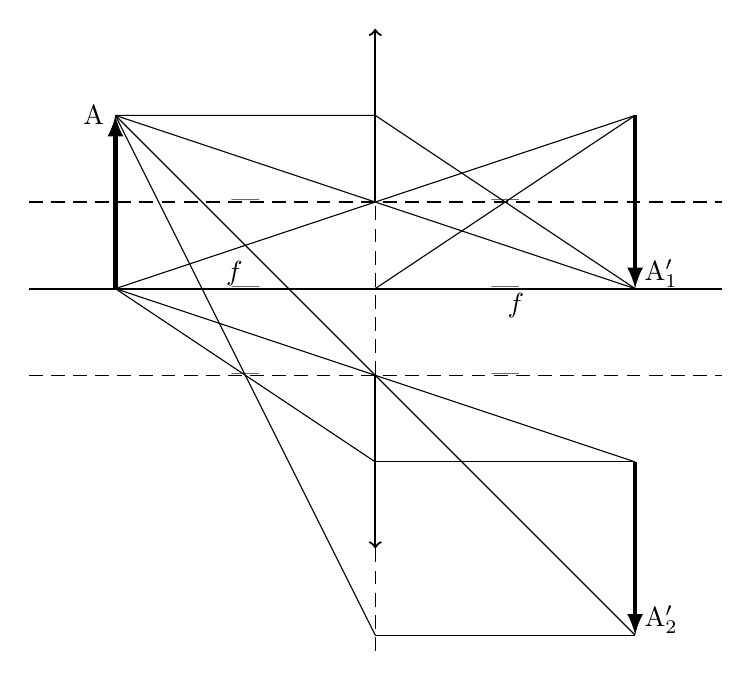
\begin{tikzpicture}[scale=0.55]

 % Def. koordinaadid
 \coordinate (O) at (0,0) ;
 \coordinate (A) at (-8,0) ;
 \coordinate (A') at (8,0) ;
 \coordinate (1) at (0,2);
 \coordinate (2) at (0,6);
 \coordinate (3) at (0,-2);
 \coordinate (4) at (0,-6);
 \coordinate (K) at (-6,4);
 \coordinate (KO) at (-6,0);
 

 % Jooned, t2pid
 \draw[thick] (A) -- (A');
 \draw[thick][->] (1) -- (2);
 \draw[thick][->] (3) -- (4);
 \draw[dash pattern=on5pt off3pt] (-8,2) -- (8,2);
 \draw[dash pattern=on5pt off3pt] (-8,-2) -- (8,-2);
 \draw[dash pattern=on5pt off3pt] (0,-2) -- (0,2);
 \draw[dash pattern=on5pt off3pt] (0, -6) -- (0,-8.5);
 \draw (K) -- (6,0);
 \draw (K) -- (0,4);
 \draw (6,0) -- (0,4);
 
 \draw (KO) -- (6,4);
 \draw (0,0) -- (6,4);
 
 \draw (KO) -- (6,-4);
 \draw (KO) -- (0,-4);
 \draw (6,-4) -- (0,-4);
 
 \draw (K) -- (6,-8);
 \draw (K) -- (0,-8);
 \draw (0,-8) -- (6,-8);
 
 \pgfsetarrowsstart{latex}
 \draw[ultra thick] (K) -- (KO) ;
 \draw[ultra thick] (6,0) -- (6,4) ;
 \draw[ultra thick] (6,-8) -- (6,-4) ;

 % Nurgad ja punktid
 \node[] at (-6.5,4) {A};
 \node[] at (-3,0) {|};
 \node[] at (3,0) {|};
 \node[] at (-3,2) {|};
 \node[] at (3,2) {|};
 \node[] at (-3,-2) {|};
 \node[] at (3,-2) {|};
 \node[] at (3.25,-0.4) {$f$};
 \node[] at (-3.25,0.35) {$f$};
 \node[] at (6.6,0.35) {$\mathrm{A_1'}$};
 \node[] at (6.6,-7.65) {$\mathrm{A_2'}$};
 
\end{tikzpicture}
\end{center}
\fi
}

% L195
\ylDisplay{Nõguspeegel} % Ülesande nimi
{EFO žürii} % Autor
{lõppvoor} % Voor
{2006} % Aasta
{G 2} % Ülesande nr.
{3} % Raskustase
{
% Teema: Geomeetriline optika

\ifSolution
Jooniselt antud kiire kahe osa pikenduste lõikepunkt vastab nõguspeegli pinnale ning kiirte nurgapoolitaja ja optilise peatelje lõikepunkt annab nõguspeegli kõverusraadiuse keskpunkti $O$. Fookuse leidmiseks paneme tähele, et nõguspeegli fookuskaugus on pool kõverusraadiusest, kus kõverusraadiuse saame mõõta jooniselt. Edasi saame fookuse kaudu konstrueerida teise punktist $A$ alguse saanud kiire käigu ning määrata eseme kujutise asukoha.

\begin{center}
	\includegraphics[width=\linewidth]{2006-v3g-02-lah}
\end{center}
\fi
}

% L196
\ylDisplay{Plaat} % Ülesande nimi
{Tundmatu autor} % Autor
{lahtine} % Voor
{2007} % Aasta
{G 4} % Ülesande nr.
{3} % Raskustase
{
% Teema: Geomeetriline optika

\ifSolution
Kiirte käik plaadis on näidatud joonisel.

\begin{center}
	\includegraphics[width=0.7\linewidth]{2007-lahg-04-lah}
\end{center}

Nurk $\angle ABC$ täisnurkses kolmnurgas $ACB$ on $\alpha$, seetõttu $|AB| = l/ \cos \alpha$. Teisest küljest, kolmnurgast $ADB$ on näha, et $|AB| = 2d \tan \gamma$. Nurgad $\alpha$ ja $\gamma$ on seotud omavahel murdumisseadusega:
\[
\frac{\sin\alpha}{\sin\gamma} = n.
\]
Lahendades need võrrandid, saame
\[
n=\frac{\sin\alpha}{\sin\left(\arctan\left(\frac{l}{2d\cos\alpha}\right)\right)} =\sin \alpha \sqrt{1+\left(\frac{2 d \cos \alpha}{l}\right)^{2}} \approx \num{1,8}.
\]
\fi
}

% L197
\ylDisplay{Kärbes} % Ülesande nimi
{Taavi Pungas} % Autor
{lahtine} % Voor
{2012} % Aasta
{G 4} % Ülesanne nr.
{3} % Raskustase
{
% Teema: Geomeetriline optika

\ifSolution
Kärbse trajektoor lühikese aja $t$ jooksul on sirgjoon pikkusega $h=vt$. Konstrueerime joonisel kärbse kujutise trajektoori. Sarnastest kolmnurkadest saame leida kujutise trajektoori pikkuse $h'$:
$$\frac{h}{a-f}=\frac{h'}{f} \Rightarrow h'=\frac{f}{a-f} h.$$
Kujutise kiirus on seega
$$v' = \frac{h'}{t} = \frac{f}{a-f} \frac{h}{t} = \frac{f}{a-f} v. $$
ning see on vastassuunaline kärbse kiirusega.
\fi
}

% L198
\ylDisplay{Peegel} % Ülesande nimi
{Oleg Košik} % Autor
{piirkonnavoor} % Voor
{2012} % Aasta
{G 1} % Ülesande nr.
{3} % Raskustase
{
% Teema: Geomeetriline optika

\ifSolution
\begin{center}
\includegraphics[width=200pt]{2012-v2g-01-peegel_lah}
\end{center}

Joonisel on kujutatud hetk $t$, mil tuttavad märkavad teineteist. Selleks hetkeks läbis $A$ teepikkuse $2-1\cdot t$ ning $B$ läbis teepikkuse $\num{3,5}-1\cdot t$. Sarnastest kolmnurkadest saame
\[
\frac{1}{\num{3,5}-t}=\frac{2-t}{1}.
\]
Tekib ruutvõrrand, mille lahenditeks on $t=\SI{1,5}{s}$ ja $t=\SI{4,0}{s}$, neist vastuseks on esimene lahend.
\fi
}

% L199
\ylDisplay{Läätsed} % Ülesande nimi
{Tanel Kiis} % Autor
{lõppvoor} % Voor
{2013} % Aasta
{G 1} % Ülesande nr.
{3} % Raskustase
{
% Teema: Geomeetriline optika

\ifSolution
\begin{center}
	\includegraphics[width=0.8\textwidth]{2013-v3g-01-laats_lah2}\\
\end{center}
Kogu pilt on optilise peatelje suhtes sümeetriline, tänu sellele saame tegeleda ainult ühe poolega. Konstrueerime kiirte käigu, teades et kõigi nõgusläätse läbivate paraleelsete kiirte pikendused lõikuvad fokaaltasandil. 

Joonisel on mõned meid huvitavad sarnased kolmnurgad: $$\Delta AF'D \sim \Delta BO'D \sim \Delta CFD$$ ja $$\Delta EOF \sim \Delta AF'O' \sim \Delta BO'F.$$ Lisaks teame osade lõikude pikkusi: $|EO| = R$, $|OF| = f_1$, $|F'O'| = f_2$ ja $|CF| = r$.
Seda teades saab moodustada neljast võrrandist koosneva lineaarvõrrandisüsteemi.
\[ 
\begin{cases}
\frac{|EO|}{|OF|} = \frac{|AF'|}{F'O}\\
\frac{|EO|}{|OF|} = \frac{|BO'|}{O'F}\\
\frac{|AF'|}{|F'D|} = \frac{|CF|}{|FD|}\\
\frac{|AF'|}{|F'D|} = \frac{|BO'|}{|O'D|},\\
\end{cases}
\]
\[ 
\begin{cases}
\frac{R}{f_1} = \frac{|AF'|}{f_2}\\
\frac{R}{f_1} = \frac{|BO'|}{\frac{f_1}{2}}\\
\frac{|AF'|}{|O'D| - f_2} = \frac{r}{\frac{f_1}{2} + |O'D|}\\
\frac{|AF'|}{|O'D| - f_2} = \frac{|BO'|}{|O'D|}.\\
\end{cases}
\]

Pärast süsteemi lahendamist saame tulemuseks $f_2 = \frac{R}{4r}f_1$. 

\vspace{0.5\baselineskip}
\emph{Alternatiivne lahendus}\\

\begin{center}
	\includegraphics[width=0.9\textwidth]{2013-v3g-01-laats_lah3}\\
\end{center}

Selles lahenduses kasutame läätse valemit $-\frac{1}{f} = \frac{1}{a} - \frac{1}{k}$. $f$ ees on miinus, kuna tegemist on nõgusläätsega, ja $k$ ees on miinus, kuna tegemist on näiva kujutisega. Kasutades kiirte pööratavuse printsiipi vaatame hoopis olukorda, kus tekib objektist $CF$ näiv kujutis $AB$. Lisaks kasutame kolmnurkade sarnasust: $\Delta CFO' \sim \Delta ABO'$ ja $\Delta DOF \sim \Delta ABF$.

\[ 
\begin{cases}
\frac{|CF|}{|FO'|} = \frac{|AB|}{|BO'|}\\
\frac{|DO|}{|OF|} = \frac{|AB|}{|BF|}\\
-\frac{1}{f_2} = \frac{1}{|FO'|} - \frac{1}{|BO'|},\\
\end{cases}
\]
\[ 
\begin{cases}
\frac{r}{\frac{f_1}{2}} = \frac{|AB|}{|BO'|}\\
\frac{R}{f_1} = \frac{|AB|}{\frac{f_1}{2} - |BO'|}\\
-\frac{1}{f_2} = \frac{1}{\frac{f_1}{2}} - \frac{1}{|BO'|}.\\
\end{cases}
\]
Selle võrrandisüsteemi lahendamisel saame $f_2 = \frac{R}{4r}f_1$.
\fi
}

% L200
\ylDisplay{Valgustamine} % Ülesande nimi
{Valter Kiisk} % Autor
{lõppvoor} % Voor
{2015} % Aasta
{G 2} % Ülesande nr.
{3} % Raskustase
{
% Teema: Geomeetriline optika

\ifSolution
Vaatleme kõige äärmiste valguskiirte liikumist läbi süsteemi. 
\begin{center}
\includegraphics[scale=1.5]{2015-v3g-02-valgustamine-lah}
\end{center}
Pärast lisaläätse läbimist koonduvad valguskiired punktiks lisaläätsest kaugusel $f_2$ ehk kaugusel $L-f_2$ algsest läätsest. Läätse valemi 
\begin{equation}
\frac{1}{a}+\frac{1}{L-f_2}=\frac{1}{f_1}.
\end{equation}
põhjal tekib sellest punktist omakorda punktkujutis kaugusele $a$ esimesest läätsest. Sarnastest kolmnurkadest saame veel kaks võrrandit:
\begin{equation}
\frac{d_1}{d_0}=\frac{L-f_2}{f_2},
\end{equation}
\begin{equation}
\frac{d}{a-f_1}=\frac{d_1}{a}.
\end{equation}
Kahest esimesest võrrandist saame suuruse $\frac{1}{L-f_2}$ avaldamisel
\begin{equation}
\frac{1}{a}+\frac{d_0}{d_1f_2}=\frac{1}{f_1}\implies \frac{d_0}{d_1f_2}=\frac{a-f_1}{af_1}.
\end{equation}
Viimasest kahest võrrandist saame avaldada suuruse $d_1(a-f_1)/a$, mille põhjal saame $d=d_0\frac{f_1}{f_2}.$ Seega valguslaigu suurus ekraanil sõltub ainult lisatud läätse fookuskaugusest, aga mitte läätsedevahelisest kaugusest $L$. Valguslaik diameetriga \SI{2}{cm} tekib kui $f_2=f_1d_0/d=\SI{2}{cm}$.
\fi
}

% L201
\ylDisplay{Valgusvihk} % Ülesande nimi
{Mihkel Kree} % Autor
{piirkonnavoor} % Voor
{2005} % Aasta
{G 5} % Ülesande nr.
{4} % Raskustase
{
% Teema: Geomeetriline optika

\ifSolution
Ülesande lahendamisel osutub tarvilikuks teadmine, et läätsele selle optilise teljega paralleelselt langevad kiired (või murtud kiirte pikendused nõgusa läätse puhul) koonduvad fookuses punktiks. Seega on ainus moodus kahe läätse abil saada süsteem, mis teisendab paralleelse kimbu uuesti paralleelseks kimbuks selline, et läätsede fookused ühtivad. 

Esimene võimalus: kasutame kahte kumerläätse. Et kimbu diameeter suureneks, peab väiksema fookuskaugusega lääts olema eespool. Lihtsast geomeetriast (sarnased kolmnurgad) ilmneb, et tekkiva kiirtekimbu diameeter on $D = df_2/f_1 = 2d$.

Teine võimalus: kasutame ühte kumerat ja ühte nõgusat läätse. Kui kumer lääts oleks esimene, siis kimbu diameeter väheneks. Seega paigutame nõgusa läätse kumera läätse ette. Nõgus lääts tekitab näilise kujutise. Kumera läätse asetame nii, et selle fookus ühtiks nõgusläätse tekitatud ebakujutise asukohaga. Sarnastest kolmnurkadest leiame, et tekib kiirekimp diameetriga
\[
D = \left|\frac{f\idx{kumer}}{f_3}d\right|.
\]
$D$ omab suurimat väärtust, kui kasutame suurema fookuskaugusega läätse, $f\idx{kumer} = f_2$. Niisiis
\[
D = \left|\frac{f_2}{f_3}d\right| = 4d.
\]


Näeme, et kiirtekimbu laiust saab suurendada maksimaalselt neli korda, kasutades selleks nõgusläätse ja kumerläätse ($f_2 = \SI{40}{cm}$) nii, et nende fookused ühtiksid.
\fi
}

% L202
\ylDisplay{Biprisma} % Ülesande nimi
{Mihkel Kree} % Autor
{piirkonnavoor} % Voor
{2006} % Aasta
{G 6} % Ülesande nr.
{4} % Raskustase
{
% Teema: Geomeetriline optika

\ifSolution
Valguskiir siseneb prismasse murdumata, sest kiir on normaali sihiline. Küll aga toimub murdumine prismast väljudes. Kuna terve tahu ulatuses on langemisnurk sama, tekitab üks tahk paralleelse kiirtekimbu (vt joonist). Kuna meil on kaks murdvat tahku, on esialgne kiirtekimp pärast prisma läbimist jagunenud kaheks.

On lihtne märgata, et langemisnurk, millega kiired langevad murdvale tahule, on $\alpha$. 
Vastavalt murdumisseadusele saame murdumisnurga $\gamma$ jaoks seose:
\[
\sin \gamma = n \sin \alpha.
\]
Väikeste nurkade jaoks lihtsustub see avaldis: $\gamma = n\alpha$. Kiir kaldus seega oma esialgsest sihist kõrvale nurga
\[
\beta = \gamma - \alpha = (n - 1) \alpha
\]
võrra. 

Teame, et paralleelne kiirtekimp koondub kumerläätse fokaaltasandis. Seega tekib fokaaltasandis asuvale ekraanile sümmeetriliselt kaks valgustäppi, teine teisele poole optilist peatelge. Arvutame ka nende kaugused peateljest. Selleks kasutame läbi läätse keskpunkti tõmmatud kiirt, mis asetseb peateljega nurga $\beta$ all. Täisnurksest kolmnurgast saame valguspunkti kauguse peateljest:
\[
s = f \tan \beta \approx f \beta = (n - 1)\alpha f.
\]
Ilmselt ei sõltu ekraanil tekkiv pilt kaugusest $d$.

Et olla päris täpne, tuleks siiski märkida, et $d$ kasvades piisavalt suureks hakkavad täpid muutuma tuhmimaks kuni lõpuks kaovad üldse, sest siis kiired enam läätse ei läbi.

\begin{center}
	\includegraphics[width=\linewidth]{2006-v2g-06-lah}
\end{center}
\fi
}

% L203
\ylDisplay{Varjud} % Ülesande nimi
{Jaak Kikas} % Autor
{piirkonnavoor} % Voor
{2007} % Aasta
{G 6} % Ülesande nr.
{4} % Raskustase
{
% Teema: Geomeetriline optika

\ifSolution
Kanname joonisele varjukoonuste piirjoonte pikendused (sirged 1-4). Valgusallikaks oleva kera lõikejoon joonise tasandiga on ringjoon, mille puutujateks on kõik need sirged. Selle keskpunkti leidmiseks konstrueerime sirgete 1-3 ja 2-4 poolt moodustatud nurkade poolitajad (punktiirjooned joonisel), nende lõikepunkt 0 on otsitava ringjoone keskpunktiks. Ringi raadiuse leidmiseks konstrueerime punktist 0 mõnele sirgetest 1-4 keskristssirge.

\begin{center}
	\includegraphics[width=\textwidth]{2007-v2g-06-lah}
\end{center}
\fi
}

% L204
\ylDisplay{Veealune valgus} % Ülesande nimi
{Jaak Kikas} % Autor
{lõppvoor} % Voor
{2008} % Aasta
{G 5} % Ülesande nr.
{4} % Raskustase
{
% Teema: Geomeetriline optika

\ifSolution
\begin{wrapfigure}{r}{0.5\textwidth}
	\begin{center}
		\includegraphics[width=0.95\linewidth]{2008-v3g-05-lah}
	\end{center}
\end{wrapfigure}
Allika heledus on ligikaudselt võrdeline vaatleja silmaava nurkläbimõõdu ruuduga allika asukohast vaadatuna. Olgu $\alpha$ ja $\alpha_0$ nurkläbimõõdud vastavalt veega täidetud ja veeta basseinis.

Jooniselt
\[
2L\tan (\alpha_0 /2) = L\tan (\alpha /2) + L\tan (\beta /2),
\]
kus langemis- ja murdumisnurkade $\alpha /2$ ja $\beta /2$ vahel kehtib seos
\[
\frac{\sin(\alpha/2)}{\sin(\beta/2)} = n.
\]
Kasutades väikeste nurkade lähendust $\tan\alpha\approx\sin\alpha\approx\alpha$, saame 
\[
\left(\frac{\alpha}{\alpha_0}\right)^2 = \frac{4n^2}{(n+1)^2}.
\]
Arvestades ka peegeldumist veepinnalt, saame heleduste suhteks
\[
\frac{I}{I_{0}}=\left(\frac{\alpha}{\alpha_0}\right)^2(1-r) = \frac{4(1-r) n^{2}}{(n+1)^{2}}=\num{1,28}.
\]
\fi
}

% L205
\ylDisplay{Konfokaalne mikroskoop} % Ülesande nimi
{Mihkel Rähn} % Autor
{lõppvoor} % Voor
{2009} % Aasta
{G 7} % Ülesande nr.
{4} % Raskustase
{
% Teema: Geomeetriline optika

\ifSolution
Lahenduse optiline skeem on toodud joonisel. Konstrueerimisel tuleb
läätsede vahelised kiired joonestada paralleelsed ja läätsede keskpunkte läbivad.
Sellisel juhul annavad need kiired eseme ja ava tasandil vastavalt eseme ja kujutise
asukohad.

\begin{center}
	\includegraphics[width=0.8\linewidth]{2009-v3g-07-G_konfokaalne_mikroskoop_lah.eps}
\end{center}

Värvitud kolmnurgad on NNN tunnuse järgi sarnased. Seetõttu kehtib võrdus
\[
\frac{d}{2f_1}=\frac{r_{\mathrm{ese}}}{f_{\mathrm{obj}}},
\]
millest
\[
r_{\mathrm{ese}}=\frac{d\cdot f_{\mathrm{obj}}}{2f_1}.
\]
\fi
}

% L206
\ylDisplay{Klaaskuulike} % Ülesande nimi
{Jaan Kalda} % Autor
{lahtine} % Voor
{2010} % Aasta
{G 4} % Ülesande nr.
{4} % Raskustase
{
% Teema: Geomeetriline optika

\ifSolution
Tagasipeegelduv kiir peegeldub kuulikeses nii, nagu näidatud joonisel. Murdumisseadusest väikeste nurkade jaoks saame
$n=\sin 2\alpha/\sin\alpha \approx 2.$
\begin{center}
	\includegraphics[width=0.35\textwidth]{2010-lahg-04-kuulike.eps}
\end{center}
\fi
}

% L207
\ylDisplay{Optiline kiud} % Ülesande nimi
{Andreas Valdmann} % Autor
{lahtine} % Voor
{2016} % Aasta
{G 4} % Ülesande nr.
{4} % Raskustase
{
% Teema: Geomeetriline optika

\ifSolution
Pikas optilises kius jäävad levima vaid sellised kiired, mille jaoks toimub südamiku ja katte lahutuspinnal täielik sisepeegeldumine. Kui valgus langeb lahutuspinnale täieliku sisepeegeldumise piirnurgast väiksema nurga all, siis toimub korraga nii peegeldumine kui ka murdumine. Pärast mitmeid peegeldusi väheneb nende kiirte intensiivsus praktiliselt nullini, sest peaaegu kogu valgus on kiu külgedelt välja murdunud. Täieliku sisepeegeldumise piirnurk 
\[
\alpha=\arcsin(n_2/n_1)=\SI{80,5}{\degree}.
\]
Piirnurgale vastavad kiired levivad kiu telje suhtes nurga $\SI{90}{\degree}-\alpha$ all. Pärast kiu otsast väljamurdumist on nende kiirte nurk kiu telje suhtes 
\[
\beta=\arcsin[n_1\sin(\SI{90}{\degree}-\alpha)]=\arcsin[n_1\cos(\alpha)].
\]
Valguskoonuse tipunurk $\theta$ on sellest kaks korda suurem: 
\[
\theta=2\beta=2\arcsin[n_1\cos(\alpha)]=\SI{28}{\degree}.
\]
Kuna $\cos(\arcsin(a))=\sqrt{1-a^2}$, siis on võimalik vastus esitada kujul 
\[
\theta=2\arcsin(\sqrt{n_1^2-n_2^2}).
\]

\begin{center}
 \includegraphics[width=0.35\textwidth]{2016-lahg-04-kiud}
\end{center}
\fi
}

% L208
\ylDisplay{Kolmlääts} % Ülesande nimi
{Andres Põldaru} % Autor
{lahtine} % Voor
{2016} % Aasta
{G 5} % Ülesande nr.
{4} % Raskustase
{
% Teema: Geomeetriline optika

\ifSolution
Kõigil kolmel läätsel on sama fookuskaugus, sest neil on üks ühine fookuspunkt, milleks on kolmnurga keskpunkt. Kolmnurgad $\triangle ACD$ ja $\triangle CEF$ on sarnased, sest nad on täisnurksed kolmnurgad, mille ühise tipu $C$ juures olevad nurgad on samad. Seega 
\[
\frac{|AD|}{|AC|}=\frac{|EF|}{|EC|},
\]
millest
\[
|AD| = \frac{|AC|}{2} = f.
\]

\begin{center}
	{\def\l{5}
	\pgfmathsetmacro\cos{cos(30)}
	\pgfmathsetmacro\tan{tan(30)}
	\begin{tikzpicture}[scale=0.7]
	\coordinate (A) at (-\l*\tan,0);
	\coordinate (B) at (\l*\cos+\l/2*\tan,0);
	\draw[Stealth-Stealth] (0,0) node[below]{C} -- ++(30:5) node[above]{E};
	\draw[Stealth-Stealth] (30:\l) -- ++(-90:5) node[below]{G};
	\draw[Stealth-Stealth] (0,0) -- ++(-30:\l);
	\draw (0,0) -- ++(210:2.5) node[below]{D} -- ++(30:0.3) arc (30:120:0.3) -- ++(-60:0.3)-- (A) -- (0,0) -- (\l*\cos,0) node[below left]{F};
	\node at (B) {\textbullet} (B) node[anchor=west] {B};
	\node at (A) {\textbullet} (A) node[anchor=east] {A};
	\draw[decorate,decoration={brace,raise=2pt,amplitude=6pt}] (A) -- node[above right = 7pt and -10pt]{$2f$} (0,0) ;
	\draw[decorate,decoration={brace,raise=2pt,amplitude=6pt}] (210:2.5) -- node[below left = 2pt and 6pt]{$f$} (A);
	\draw[decorate,decoration={brace,raise=2pt,amplitude=6pt}] (B) -- node[below right = 7pt and -8pt]{$f$} (\l*\cos,0) ;
	\end{tikzpicture}}
\end{center}

Saame järeldada, et punkt $A$ asub mõlema läätse $CE$ ja $CG$ fokaaltasandites. Kui läätsele langevad paralleelsed kiired, siis need koonduvad fokaaltasandis ühte punkti ja seega teistpidi mõeldes peavad fokaaltasandi ühest punktist pärinevad kiired olema pärast läätse läbimist paralleelsed. Nende paralleelsete kiirte nurka on võimalik määrata nii, et tõmbame punktist $A$ ühe kiire läbi läätse $CE$ või $CG$ keskpunkti. Läätse keskpunkti läbiv kiir ei murdu ja liigub samas suunas edasi. Alumisel joonisel läbib kiir $AH$ läätse keskpunkti ja teised kiired on konstrueeritud selliselt, et pärast läätse läbimist on nad sellega pralleelsed.

Pärast esimese läätse läbimist koonduvad läätsele $EG$ langevad paralleelsed kiired fokaaltasandi ühte punkti $J$. Selle punkti leidmiseks joonistame läätse $EG$ keskpunkti $F$ läbiva kiire, mis on kiirega $AH$ paralleelne, ja leiame selle kiire lõikumispunkti $J$ fokaaltasandiga. Jooniselt on näha, et ükski kiir punkti $B$ ei jõua, sest nad kõik kõik koonduvad punkti $J$ ja vertikaalseid kiiri ei ole. Läätse $CG$ jaoks on konstruktsioon sama, ainult peegelpildis $AB$ suhtes ja seega ka sealt ei jõua valgus punkti $B$.

\begin{center}
	{\def\l{5}
	\pgfmathsetmacro\cos{cos(30)}
	\pgfmathsetmacro\tan{tan(30)}
	\begin{tikzpicture}[scale=0.9]
	\usetikzlibrary{calc};
	\pgfmathsetmacro\tanb{sqrt(3)/7}
	\pgfmathsetmacro\k{\l*\cos+\l*\tan}
	\coordinate (A) at (-\l*\tan,0);
	\coordinate (B) at (\l*\cos+\l/2*\tan,0);
	\coordinate (H) at ($\k*(1,\tanb)+(A)$);
	\coordinate (J) at ($(\l*\cos,0)+\l*\tan/2*(1,\tanb)$);
	\draw[Stealth-Stealth] (0,0) node[below left]{C} -- ++(30:5) node[above]{E};
	\draw[Stealth-Stealth] (30:\l) -- ++(-90:5) node[below]{G};
	\draw[Stealth-Stealth] (0,0) -- ++(-30:5);
	\node at (B) {\textbullet} (B) node[anchor=west] {B};
	\node at (A) {\textbullet} (A) node[anchor=east] {A};
	\draw (A) -- (H) node{\textbullet} node[above left = -3pt and 0pt]{H};
	\draw (\l*\cos,0) node[left]{F} -- (J) node {\textbullet} node[above right = -5pt and 0pt]{J};
	\draw (H) -- (J);
	\draw (A) -- (30:0.5) -- ++({(\l-0.5)*\cos},{(\l-0.5)*\cos*\tanb}) -- (J);
	\draw (A) -- (30:4.5) -- ++({(\l-4.5)*\cos},{(\l-4.5)*\cos*\tanb}) -- (J);
	\end{tikzpicture}}
\end{center}

\emph{Alternatiivne lahendus}\\
Analoogselt võime vaadata hoopis seda, kui punktis $B$ on valgusallikas. Kui punktist $A$ pärinevad kiired jõuavad punkti $B$, siis peavad ka punktist $B$ pärinevad kiired jõudma punkti $A$. Punkt $B$ on läätse $EG$ fokaaltasandis ja tekitab paralleelse kiirtekimbu. Sarnaselt eelmise lahendusega see kiirtekimp koondub pärast teise läätse läbimist selle läätse fokaaltasandi ühte punkti, mis ei ole $A$. Fokaaltasand on läätsega paralleelne ja kui kiired koonduvad selles tasandis mingisse punktist $A$ erinevasse punkti, siis järelikult punkti $A$ valgus ei jõua.
\fi
}

% L209
\ylDisplay{Puuduv lääts} % Ülesande nimi
{Eero Vaher} % Autor
{piirkonnavoor} % Voor
{2017} % Aasta
{G 5} % Ülesande nr.
{4} % Raskustase
{
% Teema: Geomeetriline optika

\ifSolution
Nõguslääts tekitab esemest näiva kujutise ning kumerlääts tekitab näivast kujutisest tõelise kujutise. Teades kumerläätse asukohta ja fookuseid ning tõelise kujutise asukohta, on võimalik leida näiva kujutise asukoht (joonisel kujutatud sinisega; kujutatud on kolme kiirt, kuid konstrueerimiseks piisab kahest). Teades eseme ning nõgusläätse tekitatud näiva kujutise asukohti, on läätse asukoha ning selle esemepoolse fookuse leidmine lihtne. 

\begin{resizebox}{\linewidth}{!}{
		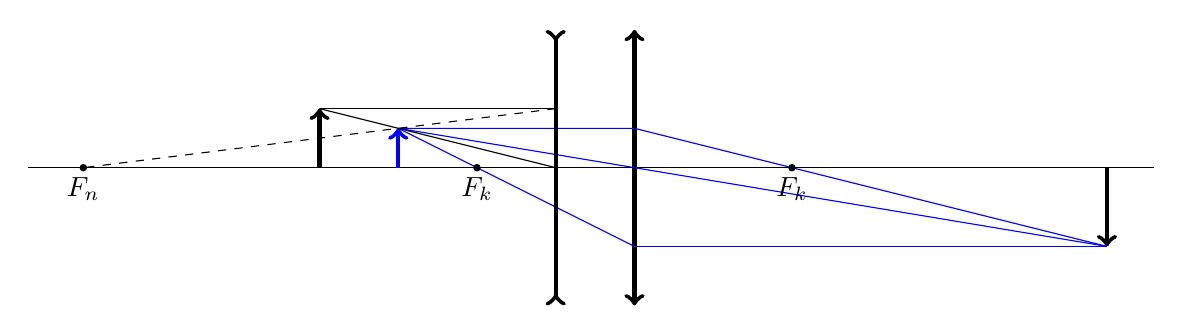
\begin{tikzpicture}
		\pgfmathsetmacro{\fk}{2}
		\pgfmathsetmacro{\tk}{3*\fk}
		\pgfmathsetmacro{\nk}{1/(1/\fk-1/\tk)}
		\pgfmathsetmacro{\a}{2*\fk}
		\pgfmathsetmacro{\h}{0.5}
		\pgfmathsetmacro{\htk}{\tk/\nk*\h}
		\pgfmathsetmacro{\ha}{1.5*\h}
		\pgfmathsetmacro{\nl}{\nk-\h/(\h-\ha)*(\nk-\a)}
		\pgfmathsetmacro{\fn}{\nk-\h/(\h-\ha)*(\nk-\nl)}
		\coordinate (TK) at (\tk, -\htk);
		\coordinate (NK) at (-\nk, \h);
		\coordinate (A) at (-\a, \ha);
		\draw (-1.1*\fn, 0) -- (1.1*\tk, 0);
		\draw[<->, ultra thick] (0,3.5*\h) -- (0,-3.5*\h);
		\draw[->, ultra thick] (\tk, 0) -- (TK);
		\draw[->, ultra thick, blue] (-\nk, 0) -- (NK);
		\draw[blue] (TK) -- (NK);
		\draw[blue] (TK) -- (0,-\htk);
		\draw[blue] (0,-\htk) -- (NK);
		\draw[blue] (TK) -- (0,\h) -- (NK);
		\draw[fill] (-\fk, 0) circle (0.02*\fk) node[below] {$F_k$};
		\draw[fill] (\fk, 0) circle (0.02*\fk) node[below] {$F_k$};
		\draw[->, ultra thick] (-\a, 0) -- (A);
		\draw[>-<, ultra thick] (-\nl, 3.5*\h) -- (-\nl, -3.5*\h);
		\draw (-\nl, 0) -- (A) -- (NK);
		\draw (A) -- (-\nl, \ha);
		\draw[dashed] (-\nl, \ha) -- (-\fn,0);
		\draw[fill] (-\fn, 0) circle (0.02*\fk) node[below] {$F_n$};
		\end{tikzpicture}}
\end{resizebox}
\fi
}

% L210
\ylDisplay{Kiilud} % Ülesande nimi
{Tundmatu autor} % Autor
{lahtine} % Voor
{2006} % Aasta
{G 6} % Ülesande nr.
{5} % Raskustase
{
% Teema: Geomeetriline optika

\ifSolution
On lihtne näha, et plaadist väljub endiselt paralleelne valgusvihk. Küll aga on selle levimise suund muutunud. Plaati sisenedes murdumist ei toimu, sest kiired liiguvad risti pinnaga. Kaldpinnale langevad kiired langemisnurga $\varphi$ all, murdumisnurga $\gamma$ saame murdumisseadusest:
\[
n_1 \sin \varphi = n_2 \sin \gamma.
\]
Meil on lubatud kasutada väikeste nurkade lähendust $\sin \alpha \approx \alpha$, mistõttu $\varphi n_1 = \gamma n_2$. Murdumise tõttu muutus kiirte levimise suund nurga $\varphi -\gamma$ võrra. Ühtlasi on lihtne näha, et see on ka langemisnurgaks plaadi välistasandile, sest esialgu liikus kiir risti plaadiga. Arvestades, et õhu murdumisnäitaja on 1, saame leida kiire murdumisnurga $\delta$ plaadist väljumisel:
\[
n_{2}(\varphi-\gamma)=\delta, \quad \delta=n_{2}\left(\varphi-\frac{\varphi n_{1}}{n_{2}}\right)=\varphi\left(n_{2}-n_{1}\right).
\]
Valguslaigu nihet on nüüd lihtne leida. Vaatleme läätse optilist keskpunkti
läbivat kiirt. Et see kiir läätses ei murdu, lõikab see fokaaltasandit teljest kaugusel
\[
d = \delta f = \varphi f (n_2 - n_1).
\]
\fi
}

% L211
\ylDisplay{Klaaskuup} % Ülesande nimi
{Tundmatu autor} % Autor
{piirkonnavoor} % Voor
{2009} % Aasta
{G 7} % Ülesande nr.
{5} % Raskustase
{
% Teema: Geomeetriline optika

\ifSolution
Mustaks värvitud tahkudelt valgus peegelduda ei saa, toimub neeldumine. Ülesande tingimus on täidetud, kui värvimata tahust kuupi sisenev valgus ei saa
väljuda läbi kõrvaltahu (toimub sisepeegeldus). Sisepeegelduse kriitilise nurga saame murdumisseadusest:
\[
\sin \gamma_{C}=\frac{1}{n}.
\]

\begin{center}
	\includegraphics[width=0.45\linewidth]{2009-v2g-07-lah}
\end{center}

Kiir siseneb kuupi, kui $\alpha<\gamma_{C}$. Langemisnurk kõrvaltahule on $\beta = \SI{90}{\degree} - \alpha$. Kiir väljub kuubist, kui
\[
\beta<\gamma_{C}, \quad \text { ehk } \quad \SI{90}{\degree}<\gamma_{C}+\alpha<2 \gamma_{C}.
\]
Et kiir ei saaks kuubist väljuda, peab kehtima:
\[
\gamma_{C}<\SI{45}{\degree}, \quad \text { ehk } \quad n>1 / \sin \SI{45}{\degree}=\sqrt{2}.
\]
\fi
}

% L212
\ylDisplay{Peeglid} % Ülesande nimi
{Jaan Kalda} % Autor
{piirkonnavoor} % Voor
{2009} % Aasta
{G 8} % Ülesande nr.
{5} % Raskustase
{
% Teema: Geomeetriline optika

\ifSolution
%Ühe peegli (nimetagem seda \enquote{esimeseks} peegliks) tasandi saab leida peegelduse $S_1$ ning selle peegelduse peegelduse $S_1^\prime$ sümmeetriateljena.
%Seejuures $S_1$ on allika $S$ peegelduseks teises peeglis ning kolmas kujutis $S_2$ on seega allika peegeldus esimeses peeglis. Niisiis, olles leidnud esimese peegli, saame
%leida ka allika asukoha --- kujutise $S_2$ peegeldusena esimeses peeglis. Peale seda saab leida ka teise peegli --- $S$ ja $S_1$ sümmeetriateljena.
%Kujutiste paariks $S_1$ ja $S_1^\prime$ saab olla ainult kaks alumist punkti joonisel, sest vastasel korral jääks valgusallikas kõigi kujutiste suhtes teisele poole esimest peeglit;
%kuivõrd teine peegel jääb $S$ ja $S_1$ vahele, siis kehtib sama %ka teise peegli jaoks ja seega ei jääks $S$ peegite vahele. Niisiis, esimeseks peegliks on kahe alumise punkti sümmeetriatelg ning allikaks ülemise punkti peegeldus selles peeglis. Teine peegel peab olema allika ja parempoolse punkti sümmeetriatelg, sest kui see oleks allika ja vasakpoolse punkti sümmeetriatelg, siis jääks allikas jällegi peeglite vahelt välja
Kuna on teada, et üks antud punktidest on peegelduse peegeldus, siis peab üks tasapeeglitest kindlasti asuma peegelduse $S_1$ ning selle peegelduse peegelduse $S_1^\prime$ sümmetriateljel. Lisaks saab punkt $S_1$ tekkida ainult siis, kui paigutada $S_1$ ja allika $S$ vahele teine peegel. Järelikult peab kolmas antud punkt $S_2$ olema allika $S$ peegeldus esimesena paigutatud peeglis, ehk see peegel asub nii $S_1$ ja $S_1^\prime$ kui ka $S$ ja $S_2$ sümmeetriateljel. Teades seda, on lihtne määrata joonisel allika $S$ asukoht. Selleks, et tekiksid peegeldused ning peegelduse peegeldused, peab allikas asuma kahe peegli vahel nii, et mõlemad peegeldavad küljed on sellele nähtavad. Kujutiste paariks $S_1$ ja $S_1^\prime$ saab olla ainult kaks alumist punkti joonisel, kuna vastasel korral jääks valgusallikas kõigi kujutiste suhtes teisele poole peegleid olenemata sellest kas $S_1$ ja $S_1^\prime$ jaoks valitakse ülemine ja vasakpoolne (joonisel $a$) või ülemine ja parempoolne (joonisel $b$).

Niisiis, esimeseks peegliks on kahe alumise punkti sümmeetriatelg ning allikaks ülemise punkti peegeldus selles peeglis. Teine peegel peab olema allika ja parempoolse punkti sümmeetriatelg, sest kui see oleks allika ja vasakpoolse punkti sümmeetriatelg, siis jääks allikas jällegi peeglite vahelt välja.\\

\begin{center}
	\includegraphics[width=0.97\linewidth]{2009-v2g-08-lah}
\end{center}
\fi
}

% L213
\ylDisplay{Periskoopprillid} % Ülesande nimi
{Andreas Valdmann} % Autor
{lõppvoor} % Voor
{2014} % Aasta
{G 4} % Ülesande nr.
{5} % Raskustase
{
% Teema: Geomeetriline optika

\ifSolution
\osa Kuna sisenevad ja väljuvad kiired on prisma pinnaga risti, siis keskkondade lahutuspiiril nende suund ei muutu. Kui kiir langeb prismale lõigul $AB$, siis peegeldub see esmalt prisma ülemisel tahul, seejärel alumisel tahul ning väljub prismast läbi parempoolse tahu (vt joonist). Kui kiir langeb prismale lõigul $BC$, siis peegeldub see ülemisel tahul, siis parempoolsel tahul ning väljub läbi alumise tahu ja ei jõuagi silma. Kui kiir langeb prismale lõigul $CD$, siis peegeldub see esmalt parempoolsel tahul, seejärel ülemisel tahul ning väljub jällegi läbi alumise tahu.

\begin{center}
 \includegraphics[width=0.8\textwidth]{2014-v3g-04-periskoopprillid_lahendus_joonis1.pdf}
\end{center}

\osa Vaatleme kiirt, mis siseneb prismasse lõigul $AB$. Kuna sisenev kiir on pinnaga risti, siis tekib täisnurkne kolmnurk $AKL$ (vt joonist). Kolmnurga üheks teravnurgaks on $\varphi$ ja seega on teise teravnurga suurus $\SI{90}{\degree}-\varphi$. Kuna viimane nurk on esimesel peegeldumisel langemisnurga täiendnurgaks, siis on ka langemisnurk $\varphi$. Peegeldumisseadusest järeldub, et esimene peegeldumisnurk on samuti $\varphi$. Kuna prismast väljuv kiir on paralleelne prisma ülemise tahuga, siis on teisel peegeldumisel peegeldumisdumisnurga täiendnurk ja seega ka langemisnurga täiendnurk $\varphi$. Näeme, et täisnurkse kolmurga $KLM$ teravnurgad on $\varphi$ ja $2\varphi$. Kuna kolmnurga sisenurkade summa on \SI{180}{\degree}, siis $\varphi=(\SI{180}{\degree}-\SI{90}{\degree})/3=\SI{30}{\degree}$.

\begin{center}
 \includegraphics[width=0.65\textwidth]{2014-v3g-04-periskoopprillid_lahendus_joonis2.pdf}
\end{center}

\emph{Märkus.} Nüüd, kui prisma tipunurk on leitud, saame veenduda, et kui pinnaga risti sisenenud kiir peegeldub prisma alumiselt või parempoolselt tahult, siis on need peegeldumised täielikud. Eelmisest alaülesandest on näha, et nendel juhtudel on langemisnurgaks $\si{90}{\degree}-\varphi=\SI{60}{\degree}$. Täieliku sisepeegeldumise piirnurk on $\alpha=\arcsin(1/n)=\SI{42}{\degree}$. Langemisnurk \si{60}{\degree} on sellest suurem ehk toimub täielik sisepeegeldumine.

\osa Kui kiir siseneb prismasse punktis $B$, siis läbib väljuv kiir punkti $D$ (vt joonist).

\emph{Märkus.} Väljuva kiire suund pole sel juhul üheselt määratud, kuid see ei oma ülesande lahendamisel tähtsust.\\
Kasutades eelmises alaülesandes saadud $\varphi$ väärtust, on näha, et kolmnurgad $ABL$ ja $BDL$ on teineteise peegeldused lõigu $BL$ suhtes (öeldakse, et need kolmnurgad on kongruentsed). Seega on lõikude $AB$ ja $BD$ pikkused võrdsed, millest järeldub, et $|AB|=l/2$. Kui kiir siseneb prismasse punktis $C$, siis peegeldub see punktis $O$ otse tagasi ning väljub prismast punktis $C$. Täisnurksetest kolmnurkadest saame, et $|AO|=\cos(\SI{30}{\degree})|AD|$ ja $|AC|=\cos(\SI{30}{\degree})|AO|$ ehk punkti $C$ kaugus punktist $A$ on 
\[
|AC|=\cos^2(\SI{30}{\degree})|AD|=\frac{3}{4}l.
\]

\begin{center}
 \includegraphics[width=0.65\textwidth]{2014-v3g-04-periskoopprillid_lahendus_joonis3.pdf}
\end{center}

\osa Ühe tasapeegli kasutamisel paistab tekst peegelpildis. Seetõttu tuleb teksti õigetpidi nägemiseks kasutada süsteemi, kus toimub paarisarv peegeldusi.
\fi
}

% L214
\ylDisplay{Lääts} % Ülesande nimi
{Mihkel Kree} % Autor
{lahtine} % Voor
{2015} % Aasta
{G 5} % Ülesande nr.
{5} % Raskustase
{
% Teema: Geomeetriline optika

\ifSolution
Paneme esmalt tähele, et läätse keskpunkti läbivad kiired AA' ja BB' ei murdu. Seega paikneb läätse keskpunkt O lõikude AA' ja BB' lõikepunktis. Teisalt märkame, et valguskiir AB murdub valguskiireks A'B'. Niisiis, pikendades lõike AB ja A'B', leiame nende lõikepunkti X. Sellega oleme konstrueerinud läätse tasandi OX. Läätse optilise peatelje leiame, kui tõmbame läätse tasandiga ristuva sirge s läbi läätse keskpunkti O. Fookuse F leidmiseks konstrueerime näiteks peateljega paralleelse kiire AC, mis murdub läbi fookuse.

\begin{center}
\includegraphics[width=\textwidth]{2015-lahg-05-laatsLahendus.pdf}
\end{center}
\fi
}

% L215
\ylDisplay{Peegelpõhi} % Ülesande nimi
{Sandra Schumann} % Autor
{lõppvoor} % Voor
{2018} % Aasta
{G 3} % Ülesande nr.
{5} % Raskustase
{
% Teema: Geomeetriline optika

\ifSolution
Paneme tähele, et valemi järgi, kui keskkonna murdumisnäitaja suureneb, aga läätse murdumisnäitaja jääb samaks, siis läätse fookuskaugus suureneb. Seega on ainus viis, kuidas valguskiired saaksid ka pärast anuma vett täis valamist samas punktis koonduda, see, kui vee sees valguskiired peegelduksid põhjas olevalt peeglilt ja seejärel koonduksid samas punktis, kus enne.

Läätse kaugus anuma põhjast on $l = \SI{10}{cm}$. Olgu läätse fookuskaugus õhus $f$. Siis on tema fookuskaugus vees järelikult $2l-f$. Valemi põhjal saame, et
\[ \frac{f}{2l-f} = \frac{n_k n_0 - n_0 n_v}{n_k n_v - n_0 n_v}\Rightarrow \]
\[ f(n_k n_v - n_0 n_v) = (2l-f)(n_k n_0 - n_0 n_v)\Rightarrow \]
\[ n_k n_v f - n_0 n_v f = 2l n_k n_0 - 2l n_0 n_v - n_k n_0 f + n_0 n_v f\Rightarrow \]
\[ f (n_k n_v + n_k n_0 - 2 n_0 n_v) = 2l n_0 (n_k - n_v)\Rightarrow \]
\[ f = \frac{2l n_0 (n_k - n_v)}{n_k n_v + n_k n_0 - 2 n_0 n_v}. \]
Seega on läätse fookuskaugus 
\[ f = \frac{\num{2} \cdot \SI{10}{cm} \cdot \num{1,0} \cdot (\num{1,49} - \num{1,33})}{\num{1,49}
\cdot \num{1,33} + \num{1,49} \cdot \num{1,0} - \num{2} \cdot \num{1,0} \cdot \num{1,33}} = \SI{3,94}{cm}
\approx \SI{4}{cm}. \]
\fi
}

% L216
\ylDisplay{Kapillaartoru} % Ülesande nimi
{Tundmatu autor} % Autor
{lahtine} % Voor
{2009} % Aasta
{G 8} % Ülesande nr.
{6} % Raskustase
{
% Teema: Geomeetriline optika

\ifSolution
\begin{center}
	\includegraphics[width=\linewidth]{2009-lahg-08-lah}
\end{center}

Et kapillaarisein paistaks null-paksusega, peab kapillaarile puutujana (punktis$A$, vt joonist) langenud kiir $a$ puudutama sisemist õõnsust (punktis $B$). Sellisel juhul pole ühtegi kiirt, mis läbiks kapillaari seina ilma sisemise õõnsuse piirpinnale langemata (ning vaid kiir $a$ teeb seda puutujana). Kolmnurk $AOB$ on täisnurkne, seetõttu saame murdumisseadusest $n= R/r$. 

Ülesande olukorda edasi analüüsides paneme tähele, et ka võrratuse $r> R/n$ korral puuduvad kiired, mis langevad kapillaari välispinnale, kuid ei lange sisemise õõnsuse piirpinnale; seega ka nende puhul näib kapillaari sein puuduvat. 

Veel paneme tähele, et igal juhul on siiski oluline erinevus ime-õhukese seinaga kapillaarist: kapillaari servale lähedaste kiirte puhul toimub täielik sisepeegeldus sisemise õõnsuse piirpinnalt (joonisel kiir $b$). Visuaalselt paistab see peegel-kihina ja on selgelt eristatav, kui nt kapillaar täita värvilise gaasiga. Samas, see sisepeegeldus kaob, kui kapillaar täita värvilise vedelikuga, mille murdumisnäitaja on $n$.
\fi
}

% L217
\ylDisplay{Fookuskaugus} % Ülesande nimi
{Eero Vaher} % Autor
{piirkonnavoor} % Voor
{2015} % Aasta
{G 8} % Ülesande nr.
{6} % Raskustase
{
% Teema: Geomeetriline optika

\ifSolution
Langegu läätsele vasakult valguskiir, mille suund on paralleelne optilise teljega ning mille kaugus sellest on $d$. Läätse sisenedes valgus oma levimissuunda ei muuda, kuna langeb läätsele selle pinnaga risti. Hõbetatud pind toimib kumerpeeglina, mille fookuskaugus on $\frac{R}{2}$. Kui peegeldunud valguskiire nurk optilise peatelje suhtes on $\alpha$, siis läätsest väljunud kiire ning optilise peatelje vaheline nurk on murdumisseaduse põhjal $\sin\gamma=n\sin\alpha$. Kuna lääts on õhuke, asetsevad punktid, kus valguskiir peegeldus ning kus see murdus, üksteisele väga lähedal. Seetõttu võime kirjutada
\[ d=\frac{R}{2}\tan\alpha=f\tan\gamma. \]
Õhukese läätse korral on selle nõgusa osa kõverusraadius oluliselt suurem fookuskaugusest, mis lubab kasutada väikeste nurkade lähendust ehk $\alpha\approx\sin\alpha\approx\tan\alpha$ ning $\gamma\approx\sin\gamma\approx\tan\gamma$. Tulemuseks saame
\[ f=\frac{R}{2n}. \]
Tasub teada, et avaldis sfäärilise peegli fookuskauguse jaoks kehtibki ainult väikeste peegeldumisnurkade korral. Suurte peegeldumisnurkade korral ilmneb sfääriline aberratsioon ning ei ole võimalik rääkida ühest fookusest.

\begin{center}
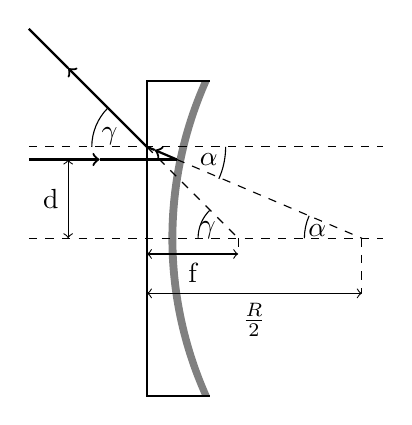
\begin{tikzpicture}[scale=1]
\def\tmp{65.92}
\fill [gray] (0.7,2) arc (90+\tmp:270-\tmp:4.9) -- (0.8,-2) -- (0.8,-2) arc (270-\tmp:90+\tmp:4.9) -- (0.7,2);
\draw[thick] (0.8,-2) -- (0,-2) -- (0,2) -- (0.8,2);
\draw[dashed] (-1.5,0) -- (3,0);
\draw[->,thick] (-1.5,1) -- (-0.6,1);
\draw[thick] (-0.6,1) -- (0.38,1);
\draw[dashed] (0.38,1) -- (2.73,0);
\draw[->,thick] (0.38,1) -- (0.1,1.12);
\draw[thick] (0.1,1.12) -- (0,1.16);
\draw[->,thick] (0,1.16) -- (-1,2.16);
\draw[thick] (-1,2.16) -- (-1.5,2.66);
\draw[dashed] (0,1.16) -- (1.16,0);
\draw[<->] (-1,0) -- (-1,1);
\node [left] at (-1,0.5) {d};
\draw[dashed] (-1.5,1.16) -- (3,1.16);
\node [left] at (-0.25,1.3) {$\gamma$};
\draw (-0.7,1.16) arc (180:135:0.7);
\node [right] at (0.55,1) {$\alpha$};
\draw (1,1.16) arc (0:-24:1);
\draw[dashed] (1.16,0) -- (1.16,-0.2);
\draw[<->] (0,-0.2) -- (1.16,-0.2);
\node [below] at (0.58,-0.2) {f}; 
\draw[dashed] (2.73,0) -- (2.73,-0.7);
\draw[<->] (0,-0.7) -- (2.73,-0.7);
\node[below] at (1.36,-0.7) {$\frac{\text{R}}{2}$};
\node[left] at (2.4,0.1) {$\alpha$};
\draw (2,0) arc (180:156:0.7);
\node[left] at (1,0.1) {$\gamma$};
\draw (0.65,0) arc (180:135:0.5);
\end{tikzpicture}
\end{center}
\fi
}

% L218
\ylDisplay{Lääts} % Ülesande nimi
{Tundmatu autor} % Autor
{lahtine} % Voor
{2007} % Aasta
{G 9} % Ülesande nr.
{7} % Raskustase
{
% Teema: Geomeetriline optika

\ifSolution
Olgu pliiatsi otste kaugused läätsest $d_1 = |BO|$ ja $d_2 = |DO|$ ning pliiatsi kujutise otste kaugused läätsest vastavalt $f_1 = |B'O|$ ja $f_2 = |D'O|$ (vt joonist).

\begin{center}
	\includegraphics[width=\linewidth]{2007-lahg-09-lah}
\end{center}

Paneme kirja valemid suurendustegurite jaoks:
\[
k=\frac{L^{\prime}}{L}, \quad k_{1}=\frac{|A^{\prime}B^{\prime}|}{|AB|}, \quad k_{2}=\frac{|C^{\prime}D^{\prime}|}{|CD|}.
\]
Sarnastest kolmnurkadest $F'B'A'$ ja $FOE$ leiame, et
\[
\frac{|A^{\prime}B^{\prime}|}{|EO|}=\frac{|F^{\prime}B^{\prime}|}{|FO|}=\frac{f_{1}-f}{f}.
\]
Analoogiliselt, sarnastest kolmnurkadest $F'D'C'$ ja $FOE$ leiame, et
\[
\frac{|C^{\prime}D^{\prime}|}{|EO|}=\frac{|F^{\prime}D^{\prime}|}{|FO|}=\frac{f_{2}-f}{f}.
\]
Kuna $|EO| = |AB| = |CD|$, siis
\[
k=\frac{f_{2}-f_{1}}{d_{1}-d_{2}}, \quad k_{1}=\frac{f_{1}-f}{f}, \quad k_{2}=\frac{f_{2}-f}{f}.
\]
Kasutades läätse valemit mõlema otsa jaoks:
\[
\frac{1}{d_{1}}+\frac{1}{f_{1}}=\frac{1}{f} \quad \operatorname{ning} \quad \frac{1}{d_{2}}+\frac{1}{f_{2}}=\frac{1}{f}
\]
saame avaldada pikkused $d_1$ ja $d_2$ pikkuste $f_1$ ja $f_2$ kaudu:
\[
d_{1}=\frac{f_{1} f}{f_{1}-f}, \quad d_{2}=\frac{f_{2} f}{f_{2}-f}.
\]
Asendame saadud väärtused suurendusteguri $k$ avaldisse:
\[
\begin{aligned}
	k&=\frac{f_{2}-f_{1}}{f_{1}-f}-\frac{f_{2} f}{f_{2}-f}=\frac{f_{2}-f_{1}}{f} \frac{\left(f_{1}-f\right)\left(f_{2}-f\right)}{f_{1}\left(f_{2}-f\right)-f_{2}\left(f_{1}-f\right)} \\ 
	&=\frac{f_{2}-f_{1}}{f} \frac{\left(f_{1}-f\right)\left(f_{2}-f\right)}{f_{1} f_{2}-f_{1} f-f_{2} f_{1}+f_{2} f}=\frac{f_{2}-f_{1}}{f} \frac{\left(f_{1}-f\right)\left(f_{2}-f\right)}{f_{2} f-f_{1} f} \\ &=\frac{f_{2}-f_{1}}{f} \frac{\left(f_{1}-f\right)\left(f_{2}-f\right)}{f\left(f_{2}-f_{1}\right)}=\frac{\left(f_{1}-f\right)\left(f_{2}-f\right)}{f^{2}}.
\end{aligned}
\]
Võrreldes saadud avaldist varem saadud avaldistega $k_1$ ja $k_2$ jaoks, on lihtne näha, et
\[
k=\frac{f_{1}-f}{f} \frac{f_{2}-f}{f}=k_{1} k_{2}.
\]
\emph{Märkus}. Joonisel me mugavuse kaalutlusel tegelikult vaatleme vaid pool pliiatsit, aga on ilmne, et lahenduskäik kehtib ka terve pliiatsi kohta (joonisel on pliiatsi teine pool näidatud punktiirjoonega).
\fi
}

% L219
\ylDisplay{Hajuti} % Ülesande nimi
{Andreas Valdmann} % Autor
{piirkonnavoor} % Voor
{2010} % Aasta
{G 8} % Ülesande nr.
{7} % Raskustase
{
% Teema: Geomeetriline optika

\ifSolution
\begin{center}
	\includegraphics[width=0.6\textwidth]{2010-v2g-08-hajuti_lah.eps}
\end{center}

Valgus läbib hajuti, kui nurk $\gamma$ on väiksem täieliku sisepeegeldumise nurgast. Kriitilisel juhul $\sin(\gamma_\mathrm{kr})=1/n$. Kuna $\beta=\SI{45}{\degree}-\gamma$, siis $\beta_\mathrm{kr} = \SI{45}{\degree}-\arcsin(1/n)$. Nurkade $\alpha$ ja $\beta$ vahel kehtib murdumisseadus $\sin(\alpha)/\sin(\beta)=n$. Seega
\[
\alpha_\mathrm{kr}=\arcsin(n\sin(\SI{45}{\degree}-\arcsin(1/n))).
\]
Vastuse saab viia kujule
\[
\alpha_\mathrm{kr}=\arcsin\left[\frac{\sqrt2}{2}(\sqrt{n^2-1}-1)\right] = \SI{4.8}{\degree}.
\]
Kriitilisest väiksema $\alpha$ korral (vt parempoolsemat kiirt) on tagasi pöörduv kiir paralleelne hajutile langenud kiirega. Kiirte käigu pööramisel selgub, et tulemus ei muutu, kui esimene sisepeegeldus toimub $45$-st kraadist suurema nurga all. Sel juhul toimub nurga $\gamma$ all teine sisepeegeldus.
\fi
}

% L220
\ylDisplay{Nõguslääts eestvaates} % Ülesande nimi
{Siim Ainsaar} % Autor
{piirkonnavoor} % Voor
{2011} % Aasta
{G 10} % Ülesande nr.
{7} % Raskustase
{
% Teema: Geomeetriline optika

\ifSolution
Kui nõgusläätsele langevad paralleelsed kiired, lõikuvad
murdunud kiirte pikendused eesmisel fokaaltasandil. Joonistame antud kiirega paralleelse abikiire (optilise kõrvaltelje, joonisel $AO$), mis läbib läätse optilist keskpunkti. See abikiir ei murdu, seega ühtib oma läätse läbimise järgse osa pikendusega. Tema lõikepunkti eesmise fokaaltasandiga (punkti $A$) leiame tõigast, et lõik $AO$ on lõigu
$KL$ paralleellüke. Küsitav murdunud kiir asub siis sirgel $AL$. Lääts asub täpselt oma
fokaaltasandite vahel keskel, seetõttu poolitab punkt $L$ lõigu $AB$, kus $B$ on küsitav murdunud kiire lõikepunkt tagumise fokaaltasandiga. Järelikult saame punkti $B$, kui peegeldame punkti $A$ punkti $L$ suhtes ($|AL| = |LB|$).

\begin{center}
	\includegraphics[width=0.5\linewidth]{2011-v2g-10-lah}
\end{center}
\fi
}

% L221
\ylDisplay{Toru} % Ülesande nimi
{Jaan Kalda} % Autor
{lõppvoor} % Voor
{2012} % Aasta
{G 6} % Ülesande nr.
{7} % Raskustase
{
% Teema: Geomeetriline optika

\ifSolution
Kõigepealt paneme tähele, et punktallika kujutis tekib läätsest kaugusele
$$l=\left(\frac 1{36}-\frac 1{60}\right)^{-1}\SI{}{mm}=\SI{90}{mm},$$
st ekraanil. Kui peegeldavate silindriliste seinte asemel oleks kaks tasapeeglit, siis
tekiks punktallika kujutiste lõpmatu jada (peegeldus, peegelduse peegeldus jne), kus 
kahe naaberkujutise vahekaugus on võrdne peeglite vahekaugusega \SI{12}{mm}. 
Läheme nüüd silindrilise juhtumi juurde. Joonise tasandis lebava kiire jaoks on 
kiirekäik täpselt sama, mis tasapeegli puhul, st joonise tasandis tekivad kujutised samuti 
perioodilise rivina, kus kujutiste vahekaugus on \SI{12}{mm}. Joonise tasandit võib pöörata suvaliselt
ümber süsteemi sümmeetriatelje; see tähendab, et kujutised on tegelikult \enquote{laiali määritud} mööda kontsentrilisi
ringjooni raadiustega $n\times\SI{12}{mm}$, kus $n$ on täisarv. Lääts tekitab neist ringidest 
ekraanile $\frac{90}{60}$ korda suurendatud kujutise, 
kus kontsentriliste ringide raadiusteks on $R=n\times \SI{18}{mm}$.
\fi
}

% L222
\ylDisplay{Mikroskoop} % Ülesande nimi
{Valter Kiisk} % Autor
{lõppvoor} % Voor
{2013} % Aasta
{G 7} % Ülesande nr.
{7} % Raskustase
{
% Teema: Geomeetriline optika

\ifSolution
Esimeses teravustatavas asendis, kus lääts on objektile lähemal kui sensorile (st suurendus $>1$), olgu läätse kaugus esemest $a$ ja sensorist $b$. Kujutise joonsuurendus on seega $k=b/a$. Teises asendis on nimetatud kaugused lihtsalt ümbervahetatud ja suurendus vastavalt $l=a/b$. Niisiis $25=k/l=b^2/a^2$.

Analüüsime nüüd esimesele asendile vastavate kauguste näitel sensori valgustatuse küsimust. Kuivõrd joonsuurendus on $k$, siis pindalamuutust iseloomustav tegur on vastavalt $k^2$. Lisaks kujutise suurusele mõjutab selle heledust ka valguse hulk, mis pääseb läbi objektiivi. Vaadeldava eseme igast punktist lähtub valgus, mis on enam-vähem ühtlaselt hajutatud üle kõigi suundade, seega läätse läbiva kiirguse hulk on proportsionaalne selle osaga mõttelise sfääri pinnast, mille lõikab välja läätse apertuur: $\Omega=d^2/a^2$, kus $d$ on läätse diameeter. Kokkuvõttes saame, et kujutise heledus on võrdeline suurusega $\Omega/k^2=d^2/b^2\propto b^{-2}$. Teises asendis, kus lääts on sensorile lähemal, on sama näitaja vastavalt $a^{-2}$, seega sel juhul on kujutise heledus suurem $a^{-2}/b^{-2}=b^2/a^2=25$ korda.
\fi
}

% L223
\ylDisplay{Optiline skeem} % Ülesande nimi
{Erkki Tempel} % Autor
{lahtine} % Voor
{2014} % Aasta
{G 7} % Ülesande nr.
{7} % Raskustase
{
% Teema: Geomeetriline optika

\ifSolution
\begin{center}
\includegraphics[width=0.7\textwidth]{2014-lahg-07-optilineskeemlahendus}
\end{center}
Algselt paralleelsed kiired koonduvad pärast läätse läbimist fokaaltasandis (punkt A). Kuna alumine kiir ei murdu, peab see läbima läätse keskpunkti. Seega lääts 1 on paralleelne joonistatud fokaaltasandiga (kiir läbib punkte A ja F) ning läbib punkti $\text{O}_1$. Kuna tegemist on kahe ühesuguse läätsega ning nende fookused asuvad punktis F, siis ring raadiusega $\text{FO}_1$ läbib alumist kiirt punktis $\text{O}_2$, mis on teise läätse keskpunktiks. Nüüd saame kergesti joonistada ka teise läätse, kuna teame ülemise kiire murdumiskohta ning läätse keskpunkti asukohta.
\fi
}

% L224
\ylDisplay{Luup} % Ülesande nimi
{Valter Kiisk} % Autor
{lõppvoor} % Voor
{2016} % Aasta
{G 6} % Ülesande nr.
{7} % Raskustase
{
% Teema: Geomeetriline optika

\ifSolution
Poolkera kumera pinna keskosa võib vaadelda omaette õhukese läätsena, mille fookuskaugus $f$ ja kaugus paberi pinnast (võrdne kumerpinna raadiusega $R$) määravad kujutise suurenduse. Selle ekvivalentse läätse fookuskauguse määramiseks vaatleme valguskiirt, mis liigub paralleelselt optilise peateljega ja pärast murdumist koondub fookusesse (vt joonis). Kui valguskiir levib optilise peatelje lähedal, siis kõik murdumisel tekkivad nurgad on väikesed, nii et saame tingimuse
\[
\alpha R\approx f\varphi.
\]
Ilmselt
\[
\varphi = \alpha - \beta=\alpha-\alpha/n=\alpha(1-1/n).
\]
Nende seoste kombineerimisel nurgad taanduvad välja ja saame $f=nR/(n-1)$. Ilmselt eseme (paberi pinna) kaugus läätsest on $R$, kusjuures $f > R$, järelikult tekib näiline kujutis kusagil paberi taga. Kõik kaugused on siiski $R$ suurusjärgus, seega suurelt distantsilt silmaga vaadeldav suurendus (st nurksuurendus) on praktiliselt sama mis joonsuurendus $y/y_0$. Kujutise konstrueerimisel tekkivatest sarnastest kolmnurkadest saame
\[
\frac{y}{y_0}=\frac{f}{f-R}=n=\num{1.5}.
\]

\begin{center}
	\includegraphics[scale=1.2]{2016-v3g-06-luup-lah}
\end{center}
\fi
}

% L225
\ylDisplay{Gravitatsioonilääts} % Ülesande nimi
{Mihkel Kree} % Autor
{piirkonnavoor} % Voor
{2007} % Aasta
{G 10} % Ülesande nr.
{8} % Raskustase
{
% Teema: Geomeetriline optika

\ifSolution
Tähest väljunud kiired kõverduvad musta augu lähiümbruses (vt joonist). 

\begin{center}
	\includegraphics[width=0.9\textwidth]{2007-v2g-10-lah1}
\end{center}

Kujutise konstrueerimisel aga eeldatakse, et kiired on kogu tee otse liikunud. Et kiired jõuavad vaatlejani kõikjalt ümber musta augu, on kujutiseks ringjoon (eeldusel, et täht on punkt).

Et silmani jõudvate kiirte jaoks kehtib $r \ll L$ ning trajektoori kõverdumine toimub tähe lähiümbruses, võib vaadelda kiire teekonda lihtsustatult: sirge liikumine musta auguni, hetkeline nurga muutus musta augu juures ning edasi sirge tee vaatlejani (vt joonist). Joonisel arusaadavalt on vertikaalskaala võrreldes horisontaalskaalaga oluliselt välja venitatud.

Järgnevalt leiame tähe nurkdiameetri. Lihtsast geomeetriast järeldub, et $\alpha + \beta = \varphi$. Kaugused on suured ning nurgad väikesed, seega võime kasutada ligikaudseid valemeid $\alpha = r/L_1$ ja $\beta = r/L_2$. Niisiis

\begin{center}
	\includegraphics[width=0.9\textwidth]{2007-v2g-10-lah2}
\end{center}

\begin{center}
	\includegraphics[width=\textwidth]{2007-v2g-10-lah3}
\end{center}

\[
\frac{r}{L_{1}}+\frac{r}{L_{2}}=\frac{4 G M}{c^{2} r} \Rightarrow r=\sqrt{\frac{4 G M L_{1} L_{2}}{c^{2}\left(L_{1}+L_{2}\right)}}.
\]
Tähe kujutise nurkdiameeter on
\[
\gamma=\frac{2 r}{L_{1}}=\sqrt{\frac{4 G M L_{2}}{c^{2} L_{1}\left(L_{1}+L_{2}\right)}}.
\]
\fi
}

% L226
\ylDisplay{Nurgapeegel} % Ülesande nimi
{Andreas Valdmann} % Autor
{lõppvoor} % Voor
{2016} % Aasta
{G 8} % Ülesande nr.
{8} % Raskustase
{
% Teema: Geomeetriline optika

\ifSolution
Vaatame kõigepealt kujutise tekkimist tasapeeglis. Joonisel 1 on olukord pealtvaates. A on Juku lahtine silm ja A$'$ selle kujutis. Kinnine silm ja selle kujutis on vastavalt B ja B$'$. Näeme, et parema silma kinnipigistamisel paistab ka peeglis kinnisena vaatleja suhtes parempoolne silm.
\begin{figure*}[h]
	\centerline{\includegraphics[scale=1.2]{2016-v3g-08-nurgapeegel_j1}}
	\caption{Kujutis tasapeeglis}
\end{figure*}

Olgu kolmest peeglist üks horisontaalne ja kaks ülejäänut vertikaalsed, kusjuures Juku vaatab otse vertikaalsete peeglite kokkupuutejoone poole. Joonisel 2 on see olukord pealtvaates. Vaatame vertikaalsete peeglite mõju. Esmalt konstrueerime silma A kujutise A$'$ vasakpoolses peeglis. Seejärel konstrueerime kujutise A$'$ kujutise A$''$ parempoolses peeglis. Toimime samamoodi kujutise B$''$ konstrueerimisel ja paneme tähele, et seekord on peegelpildil vasak ja parem pool vahetatud ning kinnisena paistab peeglites vasakpoolne silm.
\begin{figure*}[h]
	\centerline{\includegraphics[scale=1.2]{2016-v3g-08-nurgapeegel_j2}}
	\caption{Kujutis kahes peeglis}
\end{figure*}

Võtame nüüd arvesse horisontaalse peegli mõju. Joonisel 3 on otsevaates teist järku kujutis A$''$ ning selle kujutis A$'''$ horisontaalses peeglis. Näeme, et horisontaalne peegel pöörab pildi \enquote{pea peale}. Seega näeb Juku nurgapeeglis ennast sellisena, nagu on joonisel 3 kujutis A$'''$.
\begin{figure*}[h]
	\centerline{\includegraphics[scale=1.1]{2016-v3g-08-nurgapeegel_j3}}
	\caption{Peegeldumine horisontaalselt peeglilt}
\end{figure*}
\fi
}

% L227
\ylDisplay{Akvaarium} % Ülesande nimi
{Tundmatu autor} % Autor
{lahtine} % Voor
{2005} % Aasta
{G 10} % Ülesande nr.
{9} % Raskustase
{
% Teema: Geomeetriline optika

\ifSolution
\begin{center}
	\includegraphics[width=\linewidth]{2005-lahg-10-lah1}
\end{center}

\begin{center}
	\includegraphics[width=\linewidth]{2005-lahg-10-lah2}
\end{center}

Vaatleme sfäärilist akvaariumi kui õhukest tasakumerat läätse, mis on surutud tasase küljega vastu sirgeseinalist akvaariumi (vt jooniseid). Kasutades väikeste nurkade lähendust on lihtne leida sellise õhukese läätse fookuskauguse $f$ ($f = |CF|$):
\[
\gamma=\alpha n, \quad \varepsilon f=(\gamma-\alpha) f=\alpha r \quad \Rightarrow \quad f=\frac{r}{n-1}.
\]
Vee puhul
\[
f=\frac{r}{\num{1,3}-\num{1}} \approx \num{3,3} r.
\]
Läätses näeme kala kujutist, mis tekib murdumisel akvaariumivees. See kujutis on $n$ korda lähemal akvaariumi seinale, kui kala ise, st maksimaalne kaugus on
\[
l_{\max }=\frac{2 r}{n} \approx \num{1,5} r,
\]
mis on igal juhul väiksem, kui läätse fookuskaugus. Lääts tekitab sellest kujutisest omakorda kujutise, mille kauguse (läätsest) $x$ saame läätse valemist
\[
\frac{1}{f}=\frac{1}{l}-\frac{1}{x}.
\]
On lihtne näha, et suurendus on kahe kujutise kauguste suhe:
\[
\frac{1}{k}=\frac{l}{x}=1-\frac{l}{f},
\]
seega suurendus on maksimaalne, kui $l$ on maksimaalne:
\[
\frac{1}{k_{\max }}=1-\frac{2(n-1)}{n}=\frac{2-n}{n} \quad\Rightarrow\quad k_{\max }=\frac{n}{2-n} \approx \num{1,86}.
\]
\fi
}

% L228
\ylDisplay{Kuup} % Ülesande nimi
{Jaan Kalda} % Autor
{lõppvoor} % Voor
{2007} % Aasta
{G 8} % Ülesande nr.
{9} % Raskustase
{
% Teema: Geomeetriline optika

\ifSolution
Välimine ringjoon on loomulikult kera välimine kontuur, tema raadius $R_A$ on võrdne kera raadiusega foto mastaabis. Kerast eemal, piirkonnas $D$, näeb läbi kuubi põrandat, st piirkond $D$ on valge. Piirkonnas $A$ toimub täielik sisepeegeldumine kera pinnal, seega näeme me sealt põranda peegeldust, mis on samuti valge. Mõõtmise teel võib veenduda, et piirkondade $A$ ja $B$ eraldusjoone raadius $R_B$ on umbes $\sqrt 2$ korda väiksem $R_A$-st, st tegemist on põranda ja seinte eraldusjoone peegeldusega. Sestap on piirkond $B$ kollane. Piirkondade $B$ ja $C$ eraldusjoon peab vastama täieliku sisepeegeldumise lõppemisele, st piirkonnas $C$ on näha kera sisemust, mis on sinine, valge põranda taustal. Niisiis on piirkond $C$ sinine. On lihtne näha, et täieliku sisepeegeldumise piirjuhul langemisnurga siinus on $\sin \alpha = R_C/R_A = 1/n$. Seega murdumisnäitaja $n = R_A/R_C \approx \num{1,8}$.
\fi
}

% L229
\ylDisplay{Nõguspeegel} % Ülesande nimi
{Mihkel Kree} % Autor
{lõppvoor} % Voor
{2007} % Aasta
{G 9} % Ülesande nr.
{9} % Raskustase
{
% Teema: Geomeetriline optika

\ifSolution
Paneme tähele, et kõverustsenter $O$, objekt $A$ ning kujutis $A'$ kumerpeeglis asuvad samal sirgel. Seega, kui meil õnnestub leida sirge $AA'$, siis selle lõikepunkt optilise teljega annaks punkti $O$. Teisest küljest, kiir, mis läbib punkti $A$ kujutist läätses, $K_2$, ja punkti $A'$ kujutist, $K_1$, jätkub peale murdumist läätses sirgena $s'$ ja läbib nii punkti $A$ kui $A'$. Tänu sellele leiamegi sirge $AA'$ ja punkti $O$.

Punkti $A'$ leidmiseks konstrueerime esmalt fokaaltasandi $F$. Selleks leiame fokaaltasandis lebava punkti --- sirge $s$ lõikepunkti sirgega $t$, mis on paralleelne sirgega $s'$ ja läbib läätse keskpunkti. Kujutisi $K_1$ ja $K_2$ ühendav sirge murdub nii, et selle pikenduse lõikepunkt optilise peateljega ongi otsitav kõverustsenter. Punkti $A'$ leiame kui sirge $s'$ lõikepunkti sirgega $q'$, mis peale murdumist läbib fookuse ja punkti $K_1$ (sest $K_1$ on $A'$ kujutiseks).


\begin{center}
	\includegraphics[width=\linewidth]{2007-v3g-09-lah}
\end{center}
\fi
}

% L230
\ylDisplay{Kärbes} % Ülesande nimi
{Aigar Vaigu} % Autor
{piirkonnavoor} % Voor
{2008} % Aasta
{G 10} % Ülesande nr.
{9} % Raskustase
{
% Teema: Geomeetriline optika

\ifSolution
Olgu $O$ pinna kõverusraadiuse keskpunkt ning $K$ ja $A$ vastavalt kärbse näiline ja tegelik asukoht. Allpool toodud joonis kujutab kärbsest alguse saanud kahe kiire $AB$ ja $AC$ edasist käiku. Kärbse näiline asukoht $K$ vastab kärbsest alguse saanud murdunud kiirte pikenduste lõikepunktile (joonisel $KB$ ja $KC$).

Arvestades väikeste nurkade korral kehtivat lähendust $\tan \alpha \approx \sin \alpha \approx \alpha$, võime murdumisseaduse kirjutada kujul:
\[
\frac{\sin \beta}{\sin \alpha}=n \approx \frac{\beta}{\alpha}
\]
Kolmnurkade $\triangle OCB$, $\triangle ACB$ ja $\triangle KCB$ kaudu avaldame kaare $\widehat{BC}$
\[
\gamma r=\delta a=\varphi k=\widehat{BC}.
\]
Kolmnurkade $\triangle KAB$ ja $\triangle AOB$ kaudu avaldame nurga $\angle BOC$
\[
\alpha+\delta=\gamma \quad \text { ja } \quad \beta+\varphi=\gamma.
\]

\begin{center}
	\includegraphics[width=\linewidth]{2008-v2g-10-lah}
\end{center}

Saame
\[
\begin{array}{lll}{(\gamma-\alpha) a=\gamma r} & {\Rightarrow} & {\gamma(a-r)=\alpha a} \\ {(\gamma-\beta) k=\gamma r} & {\Rightarrow} & {\gamma(k-r)=\beta k.}\end{array}
\]

Paneme tähele, et need kaks võrrandit oleks saanud otse siinusteoreemist kolmnurkade $\triangle AOB$ ja $\triangle KOB$ arvestusega, et tänu nurkade $\varphi$, $\delta$ ja $\gamma$ väiksusele $|KB| \approx k$ ja $|AB| \approx a$.

Arvestades, et $\beta /\alpha \approx n$, saame
\[
\frac{a-r}{k-r}=\frac{a}{n k} \quad \Rightarrow \quad a=\frac{n r k}{n k-k+r}=\frac{\num{1,6} \cdot \num{3} \cdot \num{5}}{\num{1,6} \cdot \num{5}-\num{5}+\num{3}}=\SI{4}{mm}.
\]
\fi
}

% L231
\ylDisplay{Punktallikad} % Ülesande nimi
{Jaan Kalda} % Autor
{lõppvoor} % Voor
{2010} % Aasta
{G 9} % Ülesande nr.
{9} % Raskustase
{
% Teema: Geomeetriline optika

\ifSolution
Allikat ja kujutist ühendav sirge läheb läbi läätse keskpunkti ning see punkt peab jääma allika ja kujutise vahele, sest kujutis on tõeline.
Seetõttu saame läätse keskpunkti $O$ leida kui lõikude $S_1S_1^\prime$ ning $S_2S_2^\prime$ lõikepunkti, kus $S_1$ ja $S_2$ on allikad ning $S_1^\prime$ ja $S_2^\prime$
on vastavad kujutised. Et lõikepunkt tekiks, peavad $S_1$ ja $S_1^\prime$ paiknema diagonaalselt. Edasi paneme tähele, et sirge kujutis on sirge, kusjuures
need kaks sirget lõikuvad läätse tasandis. Et sirge $S_1S_2$ kujutis on $S_1^\prime S_2^\prime$, siis nende lõikepunkt $P$ võimaldab meil leida juba
läätse tasandi $OP$; optiline peatelg on punktist $O$ tõmmatud ristsirge Läätse tasandi seisukohast pole oluline, kumb sirgetest ($S_1S_2$ või $S_1^\prime S_2^\prime$) on kujutis ja kumb originaal.
Seetõttu tekib meil kaks oluliselt erinevat võimalust: kas need kaks sirged paiknevad ligikaudu horisontaalselt või ligikaudu vertikaalselt, vt joonist.\\

\begin{center}
	\includegraphics[width=90mm]{2010-v3g-09-punktid_lah}
\end{center}
\fi
}

% L232
\ylDisplay{Optiline süsteem} % Ülesande nimi
{Andreas Valdmann} % Autor
{lõppvoor} % Voor
{2011} % Aasta
{G 8} % Ülesande nr.
{9} % Raskustase
{
% Teema: Geomeetriline optika

\ifSolution
\begin{center}
	\includegraphics{2011-v3g-08-opt_syst1}
\end{center}

Iga süsteemile langev valguskiir murdub läätse eesmisel pinnal, peegeldub tagumisel pinnal ja murdub uuesti. Lahenduse lihtsustamiseks vaatleme olukorda, kus kiirte käik on sümmeetriline. Sel juhul langeb murdunud kiir peegelpinnale risti, peegeldub otse tagasi ja teine murdumine on esimesega identne. Süsteemi sisenev ja sealt väljuv kiir lõikavad optilist peatelge ühes ja samas punktis $P$. Seal asuva punktobjekti kujutis langeb kokku objekti endaga.

\begin{center}
	\includegraphics{2011-v3g-08-opt_syst2}
\end{center}

Võtame vaatluse alla teljelähedase kiire $PO$, mille korral võime nurga $\angle LPO$ lugeda väikeseks. Lõik $OC'$ on optilise peateljega veelgi väiksema nurga all ja punktide $O$ ning $C'$ kaugus optilisest peateljest on ligikaudu võrdne. Uurime lähemalt läätse õhukest kihti, mille kõrgus on palju väiksem kõverusraadiusest $r$. Sel juhul võime kõverpinnad asendada nende puutujatega. Pindade ristsirged on joonisel tähistatud punktiirjoonega ning need lõikavad optilist peatelge läätse kõverustsentrites. Optiline kõrvaltelg $BB'$ on paralleelne optilise peateljega ning 
\[
\angle LCO=\angle B'OC'=\angle A'OB'=\angle BOC=\angle AOB\equiv \phi
\]
ja murdumisnurk $\angle A'OC'=2\phi$. Langemisnurgaks on $\angle AOP$. Murdumisseaduse rakendamisel kasutame väikese nurga lähendust 
\[
\frac{\sin(\angle AOP)}{\sin(\angle A'OC')}=n\approx \frac{\angle AOP}{\angle A'OC'},
\]
millest
\[
\angle AOP = n \angle A'OC'=2n\phi.
\]
Järgmisteks arvutusteks on vaja teada nurka
\[
\angle LPO=\angle BOP=\angle AOP - \angle AOB=2n\phi-\phi=(2n-1)\phi.
\]
Kuna lääts on õhuke ja punkt $O$ ei ole kaugel optilisest peateljest, siis $|CO|\approx|CL|$ ja $|PO|\approx|PL|$ ning $|CL|=r-\frac{d}{2}\approx r$, kus $d$ on läätse paksus keskkohas. Jällegi väikese nurga lähendust kasutades saame
\[
|LO|=\angle LCO|CL|=\angle LPO|PL|,
\]
millest
\[
|PL|=\frac{\angle LCO}{\angle LPO}|CL|=\frac{\phi}{(2n-1)\phi} r=\frac{r}{2n-1}.
\]
Viimaseks rakendame läätse valemit
\[
\frac{1}{a}+\frac{1}{k}=\frac{1}{f}
\]
ja seost
\[
|PL|=a=k=\frac{r}{2n-1}
\]
ning saame, et
\[
f=\frac{|PL|}{2}=\frac{r}{2(2n-1)}.
\]
\fi
}

% L233
\ylDisplay{Ring ja ellips} % Ülesande nimi
{Jaan Kalda} % Autor
{lõppvoor} % Voor
{2015} % Aasta
{G 7} % Ülesande nr.
{9} % Raskustase
{
% Teema: Geomeetriline optika

\ifSolution
Läätse keskpunkt $O$ on ringile ja ellipsile tõmmatud puutujate lõikepunkt, kuna puutepunktid peavad olema originaalkujutise paarid ning neid ühendavad sirged peavad läbima läätse keskpunkti. Läätse tasandi leidmiseks valime ringil kaks punkti, $A$ ja $B$, ning leiame nende kujutised ellipsil $A'$ ja $B'$ sirgete $AO$ ja $BO$ ning ellipsi lõikepunktidena. Kui originaal on ringi kahest lõikepunktist see, mis asub läätsest kaugemal, siis selle kujutis on see, mis on läätsele lähemal (ja vastupidi), sest tõeline kujutis on pööratud tagurpidi. Kiir $AB$ peab murduma läätses kiireks $A'B'$, murdepunkt annab meile punkti $L$ läätsel ning sirge $OL$ on läätse tasandiks. Optilise peatelje $o$ leiame sirgele $OL$ punktist $O$ tõmmatud ristsirgena. Fookuse leidmiseks tõmbame punktist $A$ kiire, mis on paralleelne $o$-ga ja murdub läätsel punkti $A'$ läbivaks kiireks, mille lõikepunkt $o$-ga annab fookuse $F$.

\begin{center}
\includegraphics[width=\textwidth]{2015-v3g-07-ellips_lah}
\end{center}
\fi
}

% L234
\ylDisplay{Kaamera} % Ülesande nimi
{Ardi Loot} % Autor
{lõppvoor} % Voor
{2017} % Aasta
{G 8} % Ülesande nr.
{9} % Raskustase
{
% Teema: Geomeetriline optika

\ifSolution
On selge, et kuna virmalised asuvad kaugel, peab terava kujutise
tekkimiseks olema valgustundlik element esialgse läätse fookuses,
st kaugusel $f=\SI{14}{cm}.$ Kuna läätse keskpunkti läbiv kiir suunda
ei muuda, saame esialgseks vaatenurgaks $2\alpha=2\arctan\left(h/f\right).$

\begin{center}
	\includegraphics[width=10cm]{2017-v3g-08-skeem__telephoto.pdf}
\end{center}
Joonisel on kujutatud kompaktse kaamera skeem. Vaatleme lihtsuse huvides
olukorda tagurpidi, vaadeldav objekt asub fototundliku elemendi asemel
ning kujutis konstrueeritakse lõpmatuses (kiirte pööratavuse printsiip).
Nõguslääts, mis on paigutatud kaugusele $d$ kumerläätsest, tekitab
objektist $A$ näiva kujutise $A'$. Seda näivat kujutist vaadeldakse
kumerläätsega, mis konstrueerib sellest kujutise lõpmatuses. Kirja
saab panna järgnevad võrrandid:
\begin{eqnarray}
\frac{1}{k_{1}}-\frac{1}{a_{1}} = \frac{1}{f_{1}}, \label{2017-v3g-08-eq:telelens-eq1}\\
k_{1}+d = f_{2},\\
a_{1}+d = L_{m}.
\end{eqnarray}

\noindent Neist esimene määrab nõgusa läätse poolt näiva kujutise asukoha.
Teine võrrand garanteerib, et kumerlääts konstrueerib sellest kujutise
lõpmatuses. Kolmas võrrand tagab, et kogu süsteem oleks kompaktne.
Lisaks eeltoodud võrranditele on vaja säilitada ka esialgse kaamera
vaatenurk. Selleks märkame, et joonisel toodud nurk $\measuredangle A'O_{2}F_{2}=\alpha.$
Seetõttu saame kirja panna:
\begin{equation}
\frac{h'}{f_{2}}=\frac{h}{f},
\end{equation}
\noindent kus $h'$ tähistab kujutise $A'$ kõrgust, mille saame leida
kolmnurkade $OAO_{1}$ ja $F_{2}A'O_{1}$ sarnasusest
\begin{equation}
h'=h\frac{k_{1}}{a_{1}.}\label{2017-v3g-08-eq:telelens-eq2}
\end{equation}

Lahendades võrranditest (\ref{2017-v3g-08-eq:telelens-eq1}) - (\ref{2017-v3g-08-eq:telelens-eq2})
tekkinud süsteemi, saame
\begin{eqnarray*}
f_{1} & = & \frac{f_{2}f(L_{m}-f_{2})}{\left(f-f_{2}\right)^{2}}\approx\SI{1.39}{cm},\\
d & = & \frac{f_{2}(f-L_{m})}{f-f_{2}}\approx\SI{1.91}{cm}.
\end{eqnarray*}
\fi
}

% L235
\ylDisplay{Sähvatus} % Ülesande nimi
{Mihkel Kree} % Autor
{lõppvoor} % Voor
{2006} % Aasta
{G 9} % Ülesande nr.
{10} % Raskustase
{
% Teema: Geomeetriline optika

\ifSolution
Alustuseks paneme tähele suurepärast seost arvandmetes. Nimelt ühtivad peeglite fookused, sest peeglite vahemaa on võrdne peeglite fookuskauguste summaga. Nõguspeegli fookuskaugus on teatavasti pool raadiusest. Paralleelne kiirtekimp koondub peegli fookuses. Seepärast jääb paralleelne kiirtekimp antud süsteemis pärast kahekordset peegeldumist ikkagi paralleelseks. Kuid paneme tähele, et kiire laius väheneb kaks korda, sest ühe läätse fookuskaugus on kaks korda suurem teise omast.

Valguskiir jääb niisiis peeglite vahele pendeldama seniks, kuni tema kaugus teljest on väiksem kui $d_0/2 = \SI{0.5}{mm}$, kusjuures esialgne kauguste vahemiks, mis jõuab peegliteni on $d_2/2 = \SI{48}{mm}$ kuni $d_1/2 = \SI{80}{mm}$, ehk pilu läbimiseks peab valgusvihk koonduma $d_2/d_0 = 96$ kuni $d_1/d_0 = 160$ korda. Pärast $n$-kordset edasi-tagasi peegeldumist väheneb kiire kaugus teljest $2^n$ korda. Paneme tähele, et 128 on kahe aste ($2^7 = 128$). Seepärast väljub peeglile langenud kiir pilust kahes järgus: esimene osa pärast seitsmendat edasi-tagasi liikumist ning teine osa pärast kaheksandat. Üks edasi-tagasi liikumine peeglite vahel tekitab ajalise viivise $2L/c$.

Kumerläätsele langev paralleelne kiirtekimp koondub fookuses, kusjuures fookuseni jõudmise aeg ei sõltu kiire asukohast (teljelähedased kiired läbivad paksema klaasikihi kui kaugemad kiired, klaasi läbib valgus aga aeglasemalt). Niisiis on fookuses oodata kolme impulssi: peegli ümbert tulnud osa, pärast seitset edasi-tagasi peegeldumist tulnud osa ning pärast kaheksat. Nende impulsside ajaline vahe on vastavalt $14L/c$ ja $2L/c$.

Nüüd tuleb veel leida impulsside suhtelised intensiivsused, mis on võrdsed vastavate rõngaste pindaladega esialgse kiire ristlõikes. Esimese peegli läbimõõdust väiksem osa ei läbigi süsteemi. Kõige välimise rõnga pindala on võrdeline arvuga $192^2 - 160^2$, järgmisele impulsile vastav rõnga pindala $128^2 - 96^2$ ning viimasele impulsile vastava rõnga korral $160^2 - 128^2$. Need arvud suhtuvad kui: $32^2(6^2 - 5^2) : 32^2 (4^2 - 3^2) : 32^2 (5^2 - 4^2) = 11 : 7 : 9$.

\begin{center}
	\includegraphics[width=0.6\linewidth]{2006-v3g-09-lah}
\end{center}
\fi
}

% L236
\ylDisplay{Klaassilinder} % Ülesande nimi
{Jaan Kalda} % Autor
{lõppvoor} % Voor
{2014} % Aasta
{G 10} % Ülesande nr.
{10} % Raskustase
{
% Teema: Geomeetriline optika

\ifSolution
\begin{wrapfigure}{r}{0.35\textwidth}%
\includegraphics[trim = 0mm 0mm 12mm 0mm, clip, width=1\linewidth]{2014-v3g-10-silinder}
\end{wrapfigure}

Tähistame märgitud punkti $A$-ga ning murdugu sealt lähtunud kiir punktis $B$ nii, et suundub eemale läbi punkti $C$ (vt joonist).
Sihi $BC$ suunast kaugelt vaadatuna näeme tumeda punkti asukohana punkti $B$. Uurime, kuidas sõltub kiire $BC$ levikusuund, mida kirjeldame 
$AO$ ja $BC$ vahelise nurga $2\alpha-\beta$ abil, kiire algsest levikusuunast $\alpha$:
$$2\alpha-\beta= 2\alpha-\arcsin (n\sin\alpha).$$

Silindri algasendi korral $2\alpha-\arcsin (n\sin\alpha) =0$, mille üks lahend $\alpha=0$ annab keskmise näiva punkti
ning kaks külgmist tumedat punkti vastavad võrrandi $\sin(2\alpha)=n\sin\alpha$ ülejäänud lahenditele vahemikus $-45^\circ <\alpha<45^\circ$.
Kui pöörata nüüd silindrit nurga $\delta$ võrra, siis vastavad näivad punktid võrrandi 
$$2\alpha-\arcsin (n\sin\alpha) =\delta$$
lahenditele. Võrrandi vasakul pool on funktsioon, mis väikeste nurkade puhul käitub kui $(2-n)\alpha$; suuremate nurkade puhul teise liidetava suhteline mõju kasvab.
Seega juhul $2>n$, on tegemist väikeste nurkade puhul kasvava funktsiooniga, mis läheb suuremate nurkade puhul üle kahanevaks;
juhul $2<n$ on see aga monotoonselt kahanev funktsioon. Kuivõrd $\delta=0$ puhul on kolm lahendit, siis peab olema tegemist esimese juhtumiga, $2>n$.
Nende pöördenurkade $\delta$ puhul, mis on suuremad selle funktsiooni lokaalsest maksimumist, on võrrandil vaid üks lahend.
Funktsioon saavutab globaalse maksimumi täieliku sisepeegelduse piirjuhul 
$$n\sin\alpha=-1,$$
mis annab pöördenurga
$$90^\circ-2\arcsin \frac 1n=\SI{15}{}^\circ\Rightarrow n=1/\sin \SI{37,5}{\degree} = \SI{1,64}{}.$$
\fi
}

% L237
\ylDisplay{Autod} % Ülesande nimi
{Oleg Košik} % Autor
{piirkonnavoor} % Voor
{2006} % Aasta
{G 1} % Ülesande nr.
{1} % Raskustase
{
% Teema: Kinemaatika

\ifSolution
Vaatleme jalgratturi liikumist talle vastu sõitvate autode suhtes. Tema kiirus autode süsteemis on $v = v_1 + v_2 = \SI{120}{km/h}$. Seega katavad $n_0 = 20$ autot vahemaa $vt_0 = \SI{10}{km}$ ning terve maantee ulatuses on autosid
\[
n = n_0 \frac{s}{vt_0} = \num{360}. 
\]
\fi
}

% L238
\ylDisplay{Ummik} % Ülesande nimi
{Jaan Kalda} % Autor
{piirkonnavoor} % Voor
{2007} % Aasta
{G 2} % Ülesande nr.
{1} % Raskustase
{
% Teema: Kinemaatika

\ifSolution
Lõigul $C$ on teatud punkti ajaühikus läbivate autode arv $N_C$ võrdne lõikude $A$ ja $B$ vastavate arvude summaga: $N_C = N_A + N_B$. Olgu autode vahemaa $a$ ja vaadeldav ajavahemik $\tau$. Siis $N_i = v_i\tau /l$, ehk 
\[
\frac{v_{C} \tau}{l}=\frac{v_{A} \tau}{l}+\frac{v_{B} \tau}{l} \quad \Rightarrow \quad v_{C}=v_{A}+v_{B}.
\]
Et $v_B = L_B/t_B$, siis toodud arvude põhjal leiame 
\[
v_{B}=\frac{\SI{3}{km}}{\SI{36}{min}}=\SI{5}{km/h}
\]
ning seega $v_C = \SI{8}{km/h}$. Lõpetuseks, $t_A = L_A/v_A=\SI{20}{min}$ ja $t_C = L_C/v_ = \SI{15}{min}C$. Niisiis kulub autol aega $T = t_A + t_C = \SI{35}{min}$.
\fi
}

% L239
\ylDisplay{Auto} % Ülesande nimi
{Tundmatu autor} % Autor
{lahtine} % Voor
{2008} % Aasta
{G 1} % Ülesande nr.
{1} % Raskustase
{
% Teema: Kinemaatika

\ifSolution
Olgu $s$ läbitud vahemaa, $a$ auto kiirendus ning $\tau$ aeg, millega auto läbis esimese $4/5$ teest. Kehtivad võrdused
\[
s=\frac{a t^{2}}{2}, \quad \frac{4}{5} s=\frac{a \tau^{2}}{2}.
\]
Siit $\tau = 2t/\sqrt 5\approx \SI{13,4}{s}$. Seega otsitav ajavahemik on $t-\tau\approx \SI{1,6}{s}$.
\fi
}

% L240
\ylDisplay{Ratturid} % Ülesande nimi
{Tundmatu autor} % Autor
{lahtine} % Voor
{2009} % Aasta
{G 1} % Ülesande nr.
{1} % Raskustase
{
% Teema: Kinemaatika

\ifSolution
Olgu esimese ratturi sõiduaeg tundides $t$, siis teise ratturi sõiduaeg on $t + 1$ ning kolmanda ratturi oma $t+2$. Et esimene ja teine rattur sõitsid läbi sama pika vahemaa, saame võrrandi
\[
30 t=20(t+1),
\]
kust saame $t = \num{2}$ tundi. Järelikult linnade $A$ ja $B$ vaheline kaugus on $s = \num{30}·\num{2} = \SI{60}{km}$ kilomeetrit. Kolmanda ratturi keskmine kiirus oli seega
\[
v_{3}=\frac{s}{t+2}=\SI{15}{km/h}.
\]
\fi
}

% L241
\ylDisplay{Rong} % Ülesande nimi
{Koit Timpmann} % Autor
{piirkonnavoor} % Voor
{2013} % Aasta
{G 1} % Ülesande nr.
{1} % Raskustase
{
% Teema: Kinemaatika

\ifSolution
Olgu rongi maksimaalne kiirus $v$ ning kogu sõiduaeg $t$. Kiirendamise jooksul on keskmine kiirus $v/2$ ning sellele kulub aega $\frac{2t}{5}$. Pidurdamine võtab aega $\frac{t}{5}$ ning ka selle jooksul on keskmine kiirus $v/2$. Kogu sõidu keskmine kiirus on seega 
$$v_k = \frac{\frac{2t}{5} \frac{v}{2}+\frac{2t}{5} v + \frac{t}{5} \frac{v}{2}}{t} = \frac{7}{10} v.$$ 
Kokku,
\[
v=\frac{10}{7}v_k \approx \SI{51}{km/h}.
\]
\fi
}

% L242
\ylDisplay{Veok} % Ülesande nimi
{Valter Kiisk} % Autor
{piirkonnavoor} % Voor
{2005} % Aasta
{G 1} % Ülesande nr.
{2} % Raskustase
{
% Teema: Kinemaatika

\ifSolution
Tähistagu $x$ teepikkust, mille sõiduauto läbib möödasõidu lõpuks (vt joonist) ja olgu $t$ möödasõiduks kuluv ajavahemik. Vahemaa $x$ läbib sõiduauto ühtlase kiirendusega $a$, alustades algkiirusega $v_1$, seega
\[
x = v_1t + \frac{at^2}{2}. 
\]
Teiselt poolt, veoauto liikumise põhjal
\[
x = v_1t + L_1 + L_2 + l_1 + l_2.
\]
Kahe viimase avaldise võrdsustamisel saame
\[
\frac{a t^{2}}{2}=L_{1}+L_{2}+l_{1}+l_{2} \Rightarrow t=\sqrt{\frac{2\left(L_{1}+L_{2}+l_{1}+l_{2}\right)}{a}}\Rightarrow
\]
\[
\begin{aligned}
s &= v_1t + L_1 + L_2 + l_1 + l_2 + v_2t + l_3\\
s &= \left(v_{1}+v_{2}\right) \sqrt{\frac{2\left(L_{1}+L_{2}+l_{1}+l_{2}\right)}{a}}+L_{1}+L_{2}+l_{1}+l_{2}+l_{3} \approx \SI{349}{m}
\end{aligned}
\]

\begin{center}
	\includegraphics[width=\linewidth]{2005-v2g-01-lah}
\end{center}

\emph{Alternatiivne lahendus}

Kasutame möödasõidu aja leidmiseks veoauto taustsüsteemi, kus möödasõitva auto
algkiirus on $u = 0$:
\[
\frac{at^2}{2} = L_1 + L_2 + l_1 + l_2.
\]
Selle aja jooksul lähenevad veoauto ja vastutulev auto vahemaa
\[
s_1 = (v_1 + v_2)t 
\]
võrra, mis tähendab, et möödasõitja algvahemaa on
\[
s = s_1 + L_1 + L_2 + l_1 + l_2 + l_3 ,
\]
st (asendades $s_1$ ja $t$ eelnevatest võrranditest)
\[
s=\left(v_{1}+v_{2}\right) \sqrt{\frac{2\left(L_{1}+L_{2}+l_{1}+l_{2}\right)}{a}}+L_{1}+L_{2}+l_{1}+l_{2}+l_{3} \approx \SI{349}{m}.
\]
\fi
}

% L243
\ylDisplay{Rongiõnnetus} % Ülesande nimi
{Oleg Košik} % Autor
{piirkonnavoor} % Voor
{2011} % Aasta
{G 4} % Ülesande nr.
{2} % Raskustase
{
% Teema: Kinemaatika

\ifSolution
Teisendades kiirusühikuid, saame $v_1 = \SI{17,5}{m/s}$ ning $v_2 = \SI{5}{m/s}$. Olgu $t$ aeg, mis möödus kokkupõrkeni. Kaubarong läbis teepikkuse $s_1 = v_1t + \frac{1}{2}a_1t^2$. Elektrirong läbis teepikkuse $s_2 = v_2t + \frac{1}{2}a_2t^2$. Kuna $s = s_1 + s_2$, siis
\[
s=\left(v_{1}+v_{2}\right) t+\frac{1}{2}\left(a_{1}+a_{2}\right) t^{2}.
\]
Lahendades ruutvõrrandi, leiame $t = \SI{109}{s}$. Seega kaubarongi kiirus oli kokkupõrke hetkel $v_k = v_1 + a_1t = \SI{6,6}{m/s}$ ehk \SI{24}{km/h}, elektrirongi oma $v_e = v_2 + a_2t = \SI{21,4}{m/s}$ ehk \SI{77}{km/h}.
\fi
}

% L244
\ylDisplay{Rongivile} % Ülesande nimi
{Mihkel Kree} % Autor
{lahtine} % Voor
{2015} % Aasta
{G 1} % Ülesande nr.
{2} % Raskustase
{
% Teema: Kinemaatika

\ifSolution
Tähistagu $L$ veduri kaugust jaamaülemast hetkel, mil vedurijuht alustab vile laskmisega. Heli levimiseks jaamaülemani kulub sel juhul aeg $\tau_\text{A}=L/c$. Vile lõppedes on veduri kaugus jaamaülemast $L-vt_0$, kus $v$ on rongi liikumise kiirus. Heli levimiseks sellelt kauguselt kulub aeg $\tau_\text{B}=(L-vt_0)/c$. Alustagu vedurijuht vile laskmisega hetkel $\tau_0$ ning lõpetagu hetkel $\tau_0+t_0$. Jaamaülem kuuleb vile algust hetkel $\tau_0+\tau_\text{A}$ ning vile lõppu hetkel $\tau_0+t_0+\tau_\text{B}$. Nende ajahetkede vahe $t_1$ on mõistagi jaamaülema mõõdetud vile kestus. Seega saame võrrandi
\[
t_1 = t_0+\tau_\text{B}-\tau_\text{A} = t_0 - \frac{v}{c}t_0,
\]
millest
\[
v = \frac{t_0-t_1}{t_0}c = \SI{34}{m/s}.
\]
\fi
}

% L245
\ylDisplay{Kaubarong} % Ülesande nimi
{Erkki Tempel} % Autor
{piirkonnavoor} % Voor
{2015} % Aasta
{G 1} % Ülesande nr.
{2} % Raskustase
{
% Teema: Kinemaatika

\ifSolution
Leiame ajad, mille jooksul rong pidurdas ning kiirendas:
\[ t_p = \frac{v - v_h}{a_p},\quad t_k = \frac{v-v_h}{a_k}. \]
Rong läbis selle ajaga vahemaa
\[ s_p = \frac{v^2-v_h^2}{2a_p}, \quad s_k = \frac{v^2-v_h^2}{2a_k}. \]
Sõites ühtlaselt \SI{72}{km/h}, oleks rong läbinud selle vahemaa ajaga
\[ t_{py} = \frac{s_p}{v},\quad t_{ky} =\frac{s_k}{v}. \]
Seega aja kaotus pidurdamisel ning kiirendamisel on 
\[ \Delta t_p = t_{p} - t_{py}, \quad\Rightarrow\quad \Delta t_p = \frac{(v-v_h)^2}{2va_p}=\SI{28,125}{s},\]
\[ \Delta t_k = t_{k} - t_{ky}, \quad\Rightarrow\quad \Delta t_k = \frac{(v-v_h)^2}{2va_k}=\SI{56,25}{s}.\]
Kuna rong hilines aja $\Delta t$, siis saame leida aja $\Delta t_h$, mille rong kaotas ühtlaselt sõites:
\[ \Delta t_h = \Delta t - \Delta t_p - \Delta t_k = \SI{215,625}{s}. \]
Kui rong läbis aeglaselt (\SI{18}{km/h}) sõites vahemaa $s_h$, siis kulus tal selleks aega
\[ t_h = \frac{s_h}{v_h}. \]
Sõites kiirusega \SI{72}{km/h} oleks ta selle vahemaa läbinud ajaga
\[ t_{hy} = \frac{s_h}{v}. \]
Teades, et $\Delta t_h = t_{hy} - t_h$, saame avaldada teepikkuse $s_h$:
\[ s_h = \frac{vv_h\Delta t_h}{v-v_h} = \SI{1437,5}{m} \approx \SI{1,4}{km}.\] 
\fi
}

% L246
\ylDisplay{Kiirabiauto} % Ülesande nimi
{Sandra Schumann} % Autor
{lahtine} % Voor
{2017} % Aasta
{G 1} % Ülesande nr.
{2} % Raskustase
{
% Teema: Kinemaatika

\ifSolution
Olgu kiirabiauto kiirus $v$ ja auto poolt tekitatava heli sagedus $f_0$. Rakendame valemit kahel juhul: auto lähenemisel ja eemaldumisel.

Auto lähenemisel:
\[f_1 = \left(\frac{v_s}{v_s - v}\right)f_0.\]
Auto eemaldumisel:
\[f_2 = \left(\frac{v_s}{v_s + v}\right)f_0.\]
Kuna helisageduste erinevus kuue tooni võrra vastab kahekordsele erinevusele sagedustes, siis vastab ühetoonine erinevus $2^{\frac 1 6}$-kordsele erinevusele ja pooleteisetoonine erinevus $\left(2^{\frac 1 6}\right)^{\frac 3 2} = 2^{\frac 1 4}$-kordsele erinevusele. Seega saame:
\[2^{\frac 1 4} = \frac{f_1}{f_2} = \frac{(\frac{v_s}{v_s - v})f_0}{(\frac{v_s}{v_s + v})f_0} = \frac{v_s + v}{v_s - v},\]
\[v_s + v = 2^{\frac 1 4}v_s - 2^{\frac 1 4}v,\]
\[(2^{\frac 1 4} + 1)v = (2^{\frac 1 4} - 1)v_s,\]
\[v = \frac{2^{\frac 1 4} - 1}{2^{\frac 1 4} + 1}v_s = \frac{2^{\frac 1 4} - 1}{2^{\frac 1 4} + 1} \cdot \SI{343}{\meter\per\second} = \SI{29.64}{\meter\per\second} = \SI{107}{\kilo\meter\per\hour}. \]

Saame vastuseks \SI{107}{\kilo\meter\per\hour}.
\fi
}

% L247
\ylDisplay{Pidurdus} % Ülesande nimi
{Mihkel Rähn} % Autor
{piirkonnavoor} % Voor
{2017} % Aasta
{G 2} % Ülesande nr.
{2} % Raskustase
{
% Teema: Kinemaatika

\ifSolution
\osa Kuna autod pidurdavad maksimaalselt, siis on nende aeglustused võrdsed ning pidurdamise teepikkused on sama pikad. Seega, kui tagumise auto nina on pidurite rakendumisel samas kohas, kus eesmise auto saba oli piduritulede süttides, siis sellel piirjuhul veel otsasõitu ei toimu. Leiame vahemaa, millal see täpselt nii on:
\[
s=vt=\SI{50}{km/h}\cdot\SI{1,5}{s}=\SI{20,8}{m}.
\]
\osa Vaatleme liikumist taustsüsteemis, mis liigub kiirusega $v$ autodega samas suunas. Selles taustsüsteemis on autode esialgne kiirus null ja esimese auto pidurdamisel hakkab ta selle taustsüsteemi suhtes ühtlaselt kiirenema kiirendusega, mis on leitav seosest $F=ma$, kus $F=\mu mg$, seega $a=\mu g$. Esmalt tuleb kindlaks teha, kas kokkupõrge leiab aset enne või pärast tagumise auto pidurite rakendumist. Kui kokkupõrge toimuks enne tagumise auto pidurdama hakkamist, siis kehtiks kokkupõrke ajal $l=at^2/2$, millest
\[
t=\sqrt{2l/ug}=\SI{1.0}{s}.
\]
Kuna see on väiksem kui \num{1,5} sekundit, siis toimub autode kokkupõrge enne teise auto pidurite rakendumist autodevahelise kiirusega $\Delta v=at=\SI{36}{km/h}$.
\fi
}

% L248
\ylDisplay{Sonar} % Ülesande nimi
{Oleg Košik} % Autor
{piirkonnavoor} % Voor
{2006} % Aasta
{G 3} % Ülesande nr.
{3} % Raskustase
{
% Teema: Kinemaatika

\ifSolution
Sonarist saadetakse välja heli lainepikkusega $\lambda_1 = v_h/f_1$. Helilaine läheneb laevale kiirusega $v_h - v$, seega jõuab laevani helisignaal sagedusega
\[
f_L = \frac{v_h-v}{\lambda_1} = f_1 \frac{v_h-v}{v_h}.
\]
Peegeldudes laevalt tagasi liigub helisignaal laeva suhtes kiirusega $v_h + v$. Kuna laevalt peegeldunud kiirt saab vaadelda kui saanud alguse laeva pardalt olevalt signaaliallikalt sagedusega $f_L$, on signaali lainepikkus $\lambda_2 = (v_h+v)/f_L$. Sonari vastuvõtjasse rannikul jõuab signaal sagedusega
\[
f_{2}=\frac{v_{h}}{\lambda_{2}}=f_{L} \frac{v_{h}}{v_{h}+v}=f_{1} \frac{v_{h}-v}{v_{h}+v}.
\]
Avaldame viimasest võrdusest $v$:
\[
v = v_h \frac{f_1-f_2}{f_1+f_2}.
\]

\vspace{0.5\baselineskip}

\emph{Alternatiivne lahendus}

Kasutame Doppleri valemit
\[
f_2 = f_1 \frac{1+v_2/v_h}{1+v_1/v_h},
\]
kus saatja ja vastuvõtja lähenevad üksteisele kiirustega vastavalt $v_1$ ja $v_2$.

Kui signaal jõuab rannikult laevani, siis antud olukorras on saatja kiirus $v_1 = 0$ ja vastuvõtja kiirus $v_2 = -v$, sest vastuvõtja (laev) kaugeneb saatjast. Doppleri valem saab sel juhul kuju
\[
f_L = f_1 \frac{v_h-v}{v_h}, 
\]
kus $f_l$ on laevani jõudva signaali sagedus.

Olukorras, kus signaal läheb laevalt tagasi rannikule, on saatja kiirus $v_1 = -v$, sest saatja (laev) kaugeneb vastuvõtjast (rannikult). Vastuvõtja kiirus on aga $v_2 = 0$. Vastavalt Doppleri valemile jõuab sonari vastuvõtjasse rannikul signaal sagedusega
\[
f_2 = f_L \frac{v_h}{v_h+v} = f_1 \frac{v_h-v}{v_h+v}. 
\]
Avaldame viimasest võrdusest $v$:
\[
v = v_h \frac{f_1-f_2}{f_1+f_2}. 
\]

\emph{Märkus}. kuivõrd iga realistliku laeva kiiruse puhul $v \ll v_h$, siis on lubatud
kasutada ligikaudset Doppleri valemit
\[
f \approx f_0 \left(1+\frac{v}{v_h}\right).
\]
Sama lähendust saab kasutada ka esimese lahenduse puhul.
\fi
}

% L249
\ylDisplay{Autod} % Ülesande nimi
{Jaan Kalda} % Autor
{piirkonnavoor} % Voor
{2008} % Aasta
{G 2} % Ülesande nr.
{3} % Raskustase
{
% Teema: Kinemaatika

\ifSolution
Kanname joonisele autode $A$ ja $B$ kiirusvektorid suvalises mõõtkavas (st vektorite moodulid suhtuvad nagu 40:60). Leiame nende vektorite vahe, see on autode suhteline kiirus. Tõmmates ühe auto juurest selle vektori sihilise sirge leiame tema trajektoori teise autoga seotud süsteemis. Teise auto kaugus sellest sirgest annabki vastuse. Mõõtkava arvestamine ja mõistlik numbriline tulemus annab \SI{60}{m}.
\begin{center}
	\includegraphics[width=0.7\linewidth]{2008-v2g-02-lah}
\end{center}
\fi
}

% L250
\ylDisplay{GPS} % Ülesande nimi
{Jaan Kalda} % Autor
{lõppvoor} % Voor
{2009} % Aasta
{G 5} % Ülesande nr.
{4} % Raskustase
{
% Teema: Kinemaatika

\ifSolution
Ajahetkel $t_1=\SI{75}s$ tervisesportlane veel jooksis, sest eelmise perioodi keskmine kiirus polnud veel alanenud ($v_0=\SI{11}{km/h}$);
et ajahetkeks $t_2=\SI {90}s$ oli keskmine kiirus langenud kiiruseni $v_1=\SI{8}{km/h}$, siis oli ta seisnud juba ajavahemiku
$\tau_1$, kus $v_1 T= v_0 (T-\tau_1)$ ning $T=\SI{15}{s}$. Seega, 
\[
\tau_1=\left(1-\frac{v_1}{v_0}\right)T.
\]
Analoogselt, peale ajahetke $t_2$ seisis
sportlane veel ajavahemiku $\tau_2$, kus $v_2 T= v_3 (T-\tau_2)$ ning $v_2=\SI 3{km/h}$ ja $v_3=\SI{14}{km/h}$. Seega, 
\[
\tau_2=\left(1-\frac{v_2}{v_3}\right)T
\]
ning kogu peatusaeg
\[
\tau=\tau_1+\tau_2=T\left(2-\frac{v_1}{v_0}- \frac{v_2}{v_3}\right)\approx \SI{16}s.
\]
\fi
}

% L251
\ylDisplay{Jalgrattur} % Ülesande nimi
{Jaan Kalda} % Autor
{lõppvoor} % Voor
{2013} % Aasta
{G 3} % Ülesande nr.
{4} % Raskustase
{
% Teema: Kinemaatika

\ifSolution
Jalgratturi mõõdetav tuul $\vec w'$ on tuule kiirusvektori $\vec w$ ja jalgratturi kiirusvektori $\vec v$ vahe $\vec w'=\vec w - \vec v$. Olgu jalgratturi kiirusvektorid $\vec v_1$ ja $\vec v_2$ ning tuule kiirusvektorid $\vec w'_1$ ja $\vec w'_2$ vastavalt ühele ja teisele poole sõites.

Antud juhul teame ainult kiirusi, mitte nende suundi. Teades eelnevalt, et mõõdetud tuule kiirus on sama suur mõlemas suunas liikudes, saab kiirusvektorid esitada võrdhaarse kolmnurgana. (Kolmnurga mõlemad pooled vastavad erinevas suunas sõitmisele ning vastavad ülal mainitud valemile. Kuna tuule vektor on mõlemal juhul sama ja kiirused paralleelsed, saab selle konstrueerida nagu joonisel.)

\begin{center}
\includegraphics[width=0.4\textwidth]{2013-v3g-03-jalgrattur}\\
\end{center}

Koosinusteoreemist: 

$$
\begin{cases}
|\vec w|^2 = |\vec w'_1|^2 + |\vec v_1|^2 - 2 |\vec w'_2| |\vec v_1|\cos \alpha \\
|\vec w|^2 = |\vec w'_2|^2 + |\vec v_2|^2 - 2 |\vec w'_2| |\vec v_2|\cos \alpha.
\end{cases}
$$
Teades, et $ |\vec v_2|=2 |\vec v_1|$ ja et $ |\vec w'_1|=2 |\vec w'_2|$, saame esimese võrrandi korrutada kahega ja teise sellest lahutada.

$$|\vec w|^2 = |\vec w'_1|^2 - 2|\vec v_1|^2. $$

Ehk tuule tegelik kiirus on:
$$|\vec w|=\sqrt{|\vec w'_1|^2-2|\vec v_1|^2} \approx \SI{14}{km \per h}.$$
\fi
}

% L252
\ylDisplay{Viiul} % Ülesande nimi
{Jaan Toots} % Autor
{lõppvoor} % Voor
{2014} % Aasta
{G 2} % Ülesande nr.
{4} % Raskustase
{
% Teema: Kinemaatika

\ifSolution
Tekkival seisulainel peavad olema sõlmed mõlemas keele võnkuva osa otspunktis, seega võngub alla vajutades osa pikkusega $\frac{3}{7}L$, millele vastab lainepikkus $\lambda_0=\frac{6}{7}L$. Puudutades võngub kogu keel ning on kolm tingimust: sõlmpunktid on mõlemas otsas ning lisaks puudutatavas punktis. Seega peab sellest punktist mõlemale poole mahtuma täisarv poollainepikkusi. Võnkuvate osade suhe on $\frac{3/7}{1-3/7}$ ehk $\frac{3}{4}$. $3$ ja $4$ on ühistegurita. Seega peab jääma võnkuvatele pooltele vastavalt $3$ ja $4$ poollainepikkust. Vaadeldes pikkusega $\frac{3}{7}L$ keele poolt, taipame et $\lambda=\frac{2L}{7}$ ning
\[
\frac{\nu}{\nu_0}=\frac{\lambda_0}{\lambda}=3.
\]
\fi
}

% L253
\ylDisplay{Pöördlava} % Ülesande nimi
{Taavi Pungas} % Autor
{piirkonnavoor} % Voor
{2012} % Aasta
{G 4} % Ülesande nr.
{5} % Raskustase
{
% Teema: Kinemaatika

\ifSolution
Kettaga kaasapöörlevas taustsüsteemis peab näitleja liikuma mööda sirgjoont (et maksimeerida vahemaa).
Aja $t$ jooksul liigub ketas edasi nurga $360^\circ\frac{t}{T}=2\pi\frac{t}{T}$ võrra. Ketta peale astudes ja mööda seda kõndides saab näitleja ise edasi liikuda nurga $2\arcsin\frac{vt}{2r}$ võrra (näitleja peab jõudma tagasi ketta äärele ja sestap moodustab tema trajektoor ketta kõõlu). Kokku saame, et 
$$\alpha=360^\circ\frac{t}{T}+2\arcsin\frac{vt}{2r}=2\pi\frac{t}{T}+2\arcsin\frac{vt}{2r}.$$
\fi
}

% L254
\ylDisplay{Pallivise} % Ülesande nimi
{Eero Vaher} % Autor
{lõppvoor} % Voor
{2015} % Aasta
{G 5} % Ülesande nr.
{5} % Raskustase
{
% Teema: Kinemaatika

\ifSolution
Vaatleme palli lendu jaama teljega seotud inertsiaalses taustsüsteemis. Olgu Juku koordinaadid palli viskamise hetkel $(0,-R)$. Sellisel juhul liigub pall pärast viset ühtlaselt ning sirgjooneliselt, kusjuures selle kiiruse vertikaalsihiline komponent on $v$ ning horisontaalsihiline komponent $\omega R$. Järelikult $\tan\alpha=\frac{\omega R}{v}$, millest saame $\alpha=\frac{\pi}{3}$. Kuna kehtib $\varphi=\pi-2\alpha$, siis saame järeldada, et ka $\varphi=\frac{\pi}{3}$ ning pall läbib enne jaama pinnani jõudmist teepikkuse $R$. Palli kiirus on
\[
\sqrt{v^2+\omega^2R^2}=\frac{2\sqrt{3}}{3}\omega R,
\]
seega on pall õhus aja $t=\frac{\sqrt{3}}{2\omega}$, mille jooksul jõuab jaam pöörduda nurga $\theta=\omega t=\frac{\sqrt{3}}{2}$ võrra. Järelikult näeb Juku otse üles visatud palli maanduvat enda ees kaugusel
\[
\left(\varphi-\theta\right)R=\left(\frac{\pi}{3}-\frac{\sqrt{3}}{2}\right)R.
\]

\begin{center}
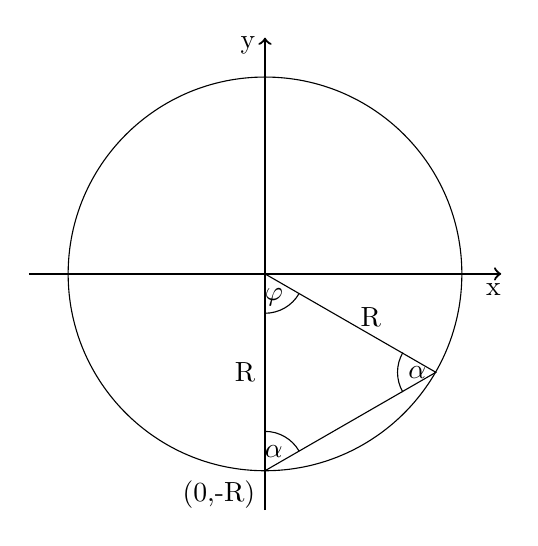
\begin{tikzpicture}[scale=1]
\draw (2.5,0) arc (0:360:2.5);
\draw[->,thick] (-3,0) -- (3,0);
\node[below] at (2.9,0) {x};
\draw[->,thick] (0,-3) -- (0,3);
\node[left] at (0,2.9) {y};
\node[left] at (0,-2.8) {(0,-R)};
\draw (0,-2.5) -- (2.17,-1.25) -- (0,0);
\node[right] at (-0.125,-2.25) {$\alpha$};
\draw (0,-2) arc (90:30:0.5);
\node[left] at (2.17,-1.25) {$\alpha$};
\draw (1.75, -1.5) arc (210:150:0.5);
\node[right] at (-0.125,-0.3) {$\varphi$};
\draw (0,-0.5) arc (270:330:0.5);
\node[left] at (0,-1.25) {R};
\node[right] at (1.09,-0.55) {R};
\end{tikzpicture}
\end{center}
\fi
}

% L255
\ylDisplay{Tsunami} % Ülesande nimi
{Jaan Kalda} % Autor
{lõppvoor} % Voor
{2005} % Aasta
{G 6} % Ülesande nr.
{6} % Raskustase
{
% Teema: Kinemaatika

\ifSolution
Laine levik toimub geomeetrilise optika seaduste kohaselt: astangu juures on laine langemisnurga ja murdumisnurga suhe
\[
\frac{\sin \alpha_{1}}{\sin \alpha_{2}}=\frac{v_{1}}{v_{2}}=\frac{\sqrt{g h_{1}}}{\sqrt{g h_{2}}}=\sqrt{\frac{h_{1}}{h_{2}}} \quad\Rightarrow\quad \alpha_{2}=\arcsin \left(\sin \alpha_{1} \sqrt{\frac{h_{2}}{h_{1}}}\right).
\]
Seal astangu osas, kus langemisnurk on \SI{0}{\degree}, murdumist ei toimu. Seal aga, kus $\alpha_1 = \SI{60}{\degree}$, on murdumisnurk
\[
\alpha_{2}=\arcsin \left(\sin \SI{60}{\degree} \sqrt{\frac{3200}{5000}}\right) \approx \SI{44}{\degree}.
\]
Seega kaldub laine esialgsest levimissuunast kõrvale nurga $\beta = \alpha_1 -\alpha_2 = \SI{16}{\degree}$ võrra. Niisiis jõuab rannalõigule $AC$ kaks lainet ning rannalõigule $DE$ ei jõua üldse lainet. Punkti $B$ jõuavad mõlemad lained üheaegselt (sümmeetria tõttu) ning seal ongi laine kõige kõrgem.

\begin{center}
	\includegraphics[width=0.6\linewidth]{2005-v3g-06-lah}
\end{center}
\fi
}

% L256
\ylDisplay{Hävituslennuk} % Ülesande nimi
{Tundmatu autor} % Autor
{lahtine} % Voor
{2011} % Aasta
{G 7} % Ülesande nr.
{6} % Raskustase
{
% Teema: Kinemaatika

\ifSolution
Olgu hetkel, mil Mati käivitab stopperi lennuki horisontaalsuunaline kaugus
temast $x_{1}$ . Tähistame lennuki lennukõrguse $H$, posti pikkuse $h$ ja
kauguse
$L$. Tekib kaks kujutletavat täisnurkset sarnast kolmnurka, mille ühise nurga
tipus asub Mati. Nendest saame (kasutades eeldust, et ilmselt $l\ll H$):
\[\frac{H-l}{x_{1}}\approx\frac{H}{x_{1}}=\frac{h-l}{L}. \]
Kui lennuk on jõudnud üle Mati pea, jõuab temani lööklaine hetkel, mil lennuki horisontaalkaugus $x_{2}$ Matist on
\[ x_{2}=\frac{H}{\tan\left(\frac{\alpha}{2}\right)}=\frac{H}{\tan\left(\arcsin\left(\frac{u}{v}\right)\right)}=\frac{H}{u}\sqrt{v^2-u^2}.
\]
Olgu $\tau$ mõõdetud aeg. Stopperi käivitamise hetkest seiskamiseni liikus lennuk vahemaa
\[ x_1+x_2=H\left(\frac{\sqrt{v^2-u^2}}{u} +\frac{L}{h-l}\right)=v\tau
\Rightarrow
H=\frac{v\tau}{\left(\frac{\sqrt{v^2-u^2}}{u} +\frac{L}{h-l}\right)}\approx
\SI{1630}{m}.
\]
\fi
}

% L257
\ylDisplay{Rehvid} % Ülesande nimi
{Siim Ainsaar} % Autor
{lõppvoor} % Voor
{2012} % Aasta
{G 5} % Ülesande nr.
{6} % Raskustase
{
% Teema: Kinemaatika

\ifSolution
\begin{wrapfigure}{r}{0.4\textwidth}
\includegraphics[width=\linewidth]{2012-v3g-05-r_joonis}
\end{wrapfigure}
Rattad tuleb pöörata suunda, mis ühtib nende liikumissuunaga. Ilmselt asub auto
pöörlemistelg tagarataste telgedega samal sirgel. Samas asub see optimaaljuhul
ka nii vasaku kui ka parema esiratta teljel. Seega otsitav nurk
\[
\beta =
\operatorname{arccot} \left( \frac{a \cot\alpha - b}{a} \right)
=
\operatorname{arccot} \left( \cot\alpha - \frac ba \right).
\]
\fi
}

% L258
\ylDisplay{Kammid} % Ülesande nimi
{Jaan Kalda} % Autor
{lõppvoor} % Voor
{2014} % Aasta
{G 5} % Ülesande nr.
{6} % Raskustase
{
% Teema: Kinemaatika

\ifSolution
Kui hall kamm liigub ühe pii võrra, on uus pilt identne esialgsega ning järelikult on tume laik liikunud ühe \enquote{lainepikkuse} võrra. 
Ühe laikude \enquote{lainepikkuse} kohta tuleb 7 halli kammi piide \enquote{lainepikkust}, seega liiguvad hallid laigud 7 korda kiiremini kui hall kamm: $v=\SI 7{cm/s}$.
\fi
}

% L259
\ylDisplay{Fotograaf} % Ülesande nimi
{Jaan Kalda} % Autor
{lõppvoor} % Voor
{2011} % Aasta
{G 6} % Ülesande nr.
{7} % Raskustase
{
% Teema: Kinemaatika

\ifSolution
Olgu pilu laius $d$, katiku kiirus $u$ ja piisa kujutise kiirus sensori tasandis $v$. Katiku
taustsüsteemis liigub piisa kujutis kiirusega $u \pm v$; kui fotoaparaat on päripidi, siis tuleb võtta märk \enquote{$+$} ja kui tagurpidi, siis \enquote{$-$}. Seega on piisa jälje tekkimise aeg
$d/|u \pm v|$ ning jälje pikkus $l = vd/|u \pm v|$. Olgu $u \geq v$; siis
\[
l_{1}=\frac{v d}{u+v}, \quad l_{2}=\frac{v d}{u-v}.
\]
Jagades teise võrrandi esimesega saame 
\[
\frac{u+v}{u-v}=\frac{l_{2}}{l_{1}}=\frac{5}{3},
\]
millest
\[
3u+ 3v = 5u-5v,
\]
ehk
\[
u = 4v.
\]
Kui fotoaparaat on portreeasendis, siis viibib piisa kujutis pilus ajavahemiku
$d/u$ jooksul ja jälje pikkus on seega
\[
l_3 = vd/u.
\]
Esimese võrrandiga läbi jagades leiame, et $l_3/l_1 = 1 + \frac{v}{u} = \frac{5}{4}$
ning
\[
l_{3}=\frac{5}{4} l_{1}=150 \text { pikselit. }
\]

Kui $u < v$, siis muutub ainult teine võrrand,
\[
l_2 = \frac{vd}{v - u},
\]
mistõttu $3u + 3v = 5v - 5u$ ja $u = v/4$, mistõttu
\[
l_{3}=5 l_{1}=600 \text { pikselit. }
\]
\emph{Märkus}. Ülesande teksti põhjal on see üks kahest võimalikust vastusest; reaalselt, arvestades tüüpilist katiku liikumiskiirust (\SI{18}{mm} läbimisaeg $\frac{1}{125}\si{s} \implies u = \SI{2,25}{m/s} \implies v = 4u = \SI{9}{m/s}$) on siiski üsna raske saavutada, et $v = 4u$: pildistamine peaks toimuma ohtlikult lähedalt. Kui joa kõrgus oleks nt \SI{100}{m}, siis vaba-langenud piisa
kiirus oleks ca \SI{44}{m/s}, mistõttu pildistamiskauguse ja objektiivi fookuskauguse suhe
(st suurendustegur) tuleks $44/9 \approx 5$ ning isegi teleobjektiivi (nt $f = \SI{300}{mm}$) korral
peaks fotograaf olema joast vaid \SI{1,5}{m} kaugusel.

\emph{Märkus 2}. Eeldusest, et \enquote{pilu laius on $d$} võib jääda mulje, justkui eeldanuks me
vaikimisi, et sensor ei jõua säritamise ajal täielikult avaneda. Ometigi kehtib lahendus
ka siis, kui säriaeg on nii pikk, et sensor jõuab täielikult avaneda: piltlikult võib
ette kujutada, et ikkagi mõlemad kardinad liiguvad samaaegselt, kuid pilu laius on
suurem sensori kõrgusest, st esimene kardin jõuab sensori kohalt eemale minna enne
teise kardina saabumist.
\fi
}

% L260
\ylDisplay{Laev} % Ülesande nimi
{Tundmatu autor} % Autor
{lõppvoor} % Voor
{2007} % Aasta
{G 5} % Ülesande nr.
{8} % Raskustase
{
% Teema: Kinemaatika

\ifSolution
Näitame, et laev peab sõitma nii, et voolukiirused stardihetkel $t_s$ ja finišihetkel $t_f$ on võrdsed, $v(t_s) = v(t_f)$. Teeme seda vastuväiteliselt. Vaatleme konkreetsuse mõttes liikumist $B$ suunas, mil laeva kiirus kalda suhtes on $v_0 + v(t)$. Sellisel juhul on läbitud vahemaa $L$ graafiku $v(t)$ ja joone $v = -v_0$ vahelise piirkonna pindala. Nihutame stardi ja finišiaega väikese ajavahemiku $\Delta t$ võrra. Läbitav vahemaa muutub seejuures $\Delta t(v_f - v_s)$ võrra. Kui $v(t_s) \neq v(t_f)$, siis saame valida $\Delta t$ märgi selliselt, et $\Delta t(v_f - v_s) > 0$, st sama aja jooksul läbitud vahemaa kasvab saades suuremaks $L$st. Seega saaks sõiduaega vähendada ning stardihetk polnud optimaalne.

Eelpoolselgitatud tingimustele (stardi- ja finišihetke kiirused on võrdsed, graafiku ja joone $v = -v_0$ vaheline pindala võrdub \SI{20}{km}-ga) vastavad stardiajad punktist $A$ 22.20 ja punktist $B$ 04.20.
\fi
}

% L261
\ylDisplay{Müra} % Ülesande nimi
{Siim Ainsaar} % Autor
{lahtine} % Voor
{2009} % Aasta
{G 10} % Ülesande nr.
{8} % Raskustase
{
% Teema: Kinemaatika

\ifSolution
% Joonis
Õhu taustsüsteemis on helilainefrondid kiirusega $c$ kasvava raadiuse ja paigaloleva keskmega poolsfäärid. Helivõimsus jaotub ühtlaselt üle terve frondipinna, seega on tajutav võimsus pöördvõrdeline frondi pindalaga ehk pöördvõrdeline frondi raadiuse ruuduga. Lisaks on võimsus ka võrdeline frontide vastuvõtmise sagedusega ehk võrdeline helisagedusega, aga nagu peagi leiame, on sagedus konstant.

\begin{wrapfigure}{r}{0.5\linewidth}
	\vspace{-10pt}
	\begin{center}
		\includegraphics[width = 0.9\linewidth]{2009-lahg-10-lah}
	\end{center}
\end{wrapfigure}

Õhu taustsüsteemis liiguvad nii matkaja kui ka jaam vastu esialgsele tuule suunale kiirusega $\beta c$. Järelikult kui front oli vastuvõtmise hetkeks raadiusega $d = ct$, siis selle kiirgamise algepunkt oli liikunud jaama suhtes allatuult kaugusele $a = (\beta c)t = \beta d$. Et see kaugus on kõigile frontidele ühesugune, on sama ka frontide teeloleku aeg ning aeg kahe frondi kiirgamise vahel võrdub ajaga nende vastuvõtmise vahel. Seega helisagedus ei muutu. Olgu jaama kaugus $\ell$. Rakendame tekkinud kolmnurgale koosinusteoreemi:
\[
d^{2}=a^{2}+\ell^{2}-2 a \ell \cos \alpha.
\]
Kuna $x = \left(\frac{\ell}{d}\right)^2$ ja $\cos \SI{135}{\degree}=-\frac{\sqrt{2}}{2}$, saame $\sqrt x$ leidmiseks ruutvõrrandi, kusjuures $\ell$ taandub välja (karakteristlik pikkusmõõde puudub).
\[
\begin{array}{c}{\frac{\ell^{2}}{x}=\frac{\beta^{2} \ell^{2}}{x}+\ell^{2}+\frac{\sqrt{2} \beta \ell^{2}}{\sqrt{x}}} \\ {x+\sqrt{2} \beta \sqrt{x}+\beta^{2}-1=0} \\ {x=\left(\frac{-\sqrt{2} \beta \pm \sqrt{2 \beta^{2}-4 \beta^{2}+4}}{2}\right)^{2}=\frac{\left(-\beta \pm \sqrt{2-\beta^{2}}\right)^{2}}{2}=1 \mp \beta \sqrt{2-\beta^{2}}.}\end{array}
\]
Heli jääb vaiksemaks, mistõttu $x < 1$ ja peame valima miinusmärgiga lahend
\[
x=1-\beta \sqrt{2-\beta^{2}}.
\]
\fi
}

% L262
\ylDisplay{Kaater} % Ülesande nimi
{Jaan Kalda} % Autor
{lõppvoor} % Voor
{2009} % Aasta
{G 8} % Ülesande nr.
{8} % Raskustase
{
% Teema: Kinemaatika

\ifSolution
\osa
Veega seotud taustsüsteemis liiguvad lained paadi trajektoori suhtes sümmeetriliselt. Seega, veega seotud taustsüsteemis on
paadi trajektoor lainetest moodustatud nurga poolitaja. Paadi kiirusest $\vec u$, jõe voolukiirusest $\vec v$ ja paadi kiirusest maa suhtes moodustub kiiruste kolmnurk, vt joonis.
Jooniselt mõõdame selle kolmnurga teravama nurga siinuse, $\sin \alpha =v/u=\num{0.26}$, millest $v=\SI{1.8}{m/s}$.

\begin{center}
	\includegraphics[width=0.8\linewidth]{2009-v3g-08-paatlah.eps}
\end{center}

\osa
Kui paat tekitas teatud punktis häirituse, siis levis see ajaga $t$ kaugusele $wt$ (nähtavaks paadilaineks on selliste ringide mähisjoon),
paat aga liikus kaugusele $ut$. Seega leiame jooniselt pikkuste suhte abil $w/u=|OP|/|OQ|=\num{0.64}$, millest $w=\SI{4.5}{m/s}$. Järelikult on vee sügavus
$h=w^2/g=2\,$m.
\fi
}

% L263
\ylDisplay{Päikese pöörlemine} % Ülesande nimi
{Mihkel Kree} % Autor
{lahtine} % Voor
{2014} % Aasta
{G 10} % Ülesande nr.
{8} % Raskustase
{
% Teema: Kinemaatika

\ifSolution
Olgu Päikese pöörlemise joonkiirus ekvaatoril $v$. Kuna punktid A ja B lähenevad meile ja kaugenevad meist kiirusega $v$, siis mõõdetavad lainepikkused $\lambda_\text{A}$ ja $\lambda_\text{B}$ erinevad algsest lainepikkusest $\lambda_0$ Doppleri nihke tõttu. Punktist A näib kiirguvat lühem lainepikkus $\lambda_\text{A}=\lambda_0(1-v/c)$ ning punktist B pikem $\lambda_\text{B}=\lambda_0(1+v/c)$.

Kes Doppleri valemit peast ei tea, võib arutleda ka järgnevalt. Liikugu kiirguse allikas meie poole kiirusega $v$. Lainepikkusele $\lambda_0$ vastava laine sagedus on $f_0=\frac{c}{\lambda_0}$, järelikult võime mõelda, et lainehari kiiratakse iga intervalli $\tau = 1/f_0 = \lambda_0/c$ järel, mis vastab laine perioodile. Kiiratagu mingil hetkel esimene lainehari. Ühe perioodi jooksul liigub see kaugusele $x=c\tau$; allikas ise liigub aga selle aja jooksul meile lähemale $\Delta x = v\tau$ võrra ja kiirgab sealt järgmise laineharja. Niisiis tundub meile kui vaatlejale, et kahe laineharja vaheline kaugus ehk lainepikkus on 
\[
\lambda'=x-\Delta x=(c-v)\tau = \lambda_0(1-v/c).
\]

Punktidest A ja B mõõdetud lainepikkuste erinevus avaldub niisiis kui 
\[
\Delta\lambda = \lambda_\text{B}-\lambda_\text{A} = 2\lambda_0 v/c,
\]
kust saame lihtsalt avaldada joonkiiruse $v=c\Delta\lambda/2\lambda_0$ ning selle abil ka pöörlemisperioodi:
\[
T_\text{p}=\frac{2\pi r}{v}=\frac{4 \pi r \lambda_0}{c\Delta \lambda}=
\frac{4 \cdot 3.14 \cdot 7\cdot 10^8 \cdot 5.9 \cdot 10^{-7}}{3\cdot 10^8\cdot 7.8\cdot 10^{-12}}\,\text{s}\approx \SI{26}{\textit{T}_\text{m}}.
\]
Päike ei ole tahke keha, selle erinevad laiuskraadid pöörlevad erineva nurkkiirusega. Pooluselähedastel piirkondadel kulub ühe täispöörde tegemiseks umbes 34 päeva.
\fi
}

% L264
\ylDisplay{Traatrõngad} % Ülesande nimi
{Jaan Kalda} % Autor
{lõppvoor} % Voor
{2014} % Aasta
{G 9} % Ülesande nr.
{8} % Raskustase
{
% Teema: Kinemaatika

\ifSolution
Läheme süsteemi, mis pöörleb nurkkiirusega $\omega/2$; seal on näha, et lõikepunkt ei pöörle, vaid liigub radiaalselt.
Seega, laboratoorses süsteemis on selle nurkkiirus $\omega/2$; sellise nurkkiirusega pöörleb kõõl $AB$; et kesknurk on kahekordne piirdenurk, siis 
raadius $OB$ (kus $O$ on seisva rõnga keskpunkt) pöörleb nurkkiirusega $\omega$ ning järelikult on lõikepunkti kiirus samaselt võrdne $\omega R$-ga.
\fi
}

% L265
\ylDisplay{Kodarad} % Ülesande nimi
{Tundmatu autor} % Autor
{lahtine} % Voor
{2011} % Aasta
{G 10} % Ülesande nr.
{9} % Raskustase
{
% Teema: Kinemaatika

\ifSolution
Kodara antud punkt näib kujutisel terav, kui selle kiirusvektor on suunatud pikki kodarat, st antud punktis kodar ei liigu enese ristsihis.

\begin{wrapfigure}{r}{0.3\textwidth}
	\vspace*{-15pt}
	\includegraphics[width=0.3\textwidth]{2011-lahg-10-kodar_a}
	\vspace*{-25pt}
\end{wrapfigure}

Olukorda võib selgitada juuresoleva joonise abil.
Olgu $R$ ratta raadius ja olgu selle keskpunt $O$. Kui kodara pöördenurk on $\theta$ ning see nurk muutub pildistamise jooksul nurga $\D\theta$ võrra,
siis $O$ on läbinud teatud vahemaa ($R \, \D\theta$), aga kodar on samuti pöördunud sama nurga ($\D \theta$) võrra.
Jooniselt on näha, et uuel ja vanal kodara asendil on üks ühine punkt, olgu see punkt $Q$. Nii pildistamise alg- kui ka lõpphetkel asus selles punktis kodar, mistõttu kujutisel jääb see punkt selgelt näha (erinevalt teistest punktidest, kus kodar viibis vaid lühiajaliselt).

Kasutades eeltoodud joonist (kus tähistasime $OQ = r$) võime avaldada lõigu $MN$
pikkuse kahel viisil: $R \,\D \theta \cos \theta = r \,\D \theta$, kus
paremal pool kasutasime väikese nurga lähendust $\sin \D\theta\approx \D\theta$. Seega $R \cos \theta = r$, mis tähendab, et
(a) punkt $Q$ on leitav kodara lõikepunktina ratta ja maa kontaktpunktist $S$ kodarale tõmmatud ristsirgega (vt järgnev joonis);
(b) vaadeldes seda võrdust kui raadiuse $r$ sõltuvust polaarnurgast $\theta$ näeme, et ülejäänud kodarate teravalt kujutuvad punktid asuvad ringjoonel,
mille diameetriks on ratta raadius $OS$.

\vspace{0.5\baselineskip}

\textit{Alternatiivne lahendus}

Pildistamise hetkel pöörleb kogu ratas ümber hetkelise pöörlemistelje, mis läbib
ratta ja maa puutepunkti $S$ (vt. joonist). Sellel hetkel liigub iga ratta osake
mööda ringjoone kaart, mille keskpuntiks on $S$. Kui ühe sellisel moel liikuva
punkti kiirus on mööda kodarat ($OP$), siis see punkt kujutub fotol selgena.
Seega me otsime selliseid punkte $Q$, mille juures $\angle OQS$ on täisnurk.
Piirdenurga omaduse põhjal peab selline punkt $Q$ lebama ringjoonel, mille
diameetriks on $OS$ --- sõltumata kodara kaldenurgast $\theta$.
\begin{center}
	\includegraphics[width=0.65\textwidth]{2011-lahg-10-kodar_b}
\end{center}
\fi
}

% L266
\ylDisplay{Anemomeeter} % Ülesande nimi
{Jaan Kalda} % Autor
{lahtine} % Voor
{2016} % Aasta
{G 9} % Ülesande nr.
{9} % Raskustase
{
% Teema: Kinemaatika

\ifSolution
Leviaegade suhtelised erinevused on väikesed, seega võime lugeda, et helikiirus on hulga suurem tuule kiirusest.
Vaatleme heli levikut õhuga seotud taustsüsteemis, kus sensorite suhtelise nihke $x$- ja $y$-telje sihilised komponendid ($s_x=u_x\frac a{c_s}$ ja 
$s_y=u_y\frac a{c_s}$) on samuti väikesed: $s_x, s_y\ll a$; $u_x$ ja $u_y$ tähistavad tuule kiiruse komponente ning $c_s$ - heli kiirust.
Rangelt võttes pidanuksid siin valemeis olema täpsed lennuajad $t_A$, $t_B$ ja $t_C$, kuid nihked ise on väikesed ning leviaegade 
väikeste vahede tõttu tuleb viga juba tühiselt väike. Niisiis saame leviaegade jaoks avaldised:
\begin{align*}
t_A&=\frac 1{c_s}\left(a+u_y\frac a{c_s}\right),\\
t_B&=\frac 1{c_s}\left(a+u_x\frac a{c_s}\right)\;\; \mbox{ja}\\
t_C&=\frac 1{c_s}\left(a-u_x\frac a{c_s}\right),
\end{align*}
millest $ \frac a{c_s}=\frac 12(t_B+t_C)$, $$u_x=\frac {c_s^2}a\left[t_B-\frac 12(t_B+t_C)\right]=c_s\frac{t_B-t_C}{t_B+t_C}=2a\frac{t_B-t_C}{(t_B+t_C)^2}\approx \SI{6.1}{m/s}$$
ning 
$$u_y=\frac {c_s^2}a\left[t_A-\frac 12(t_B+t_C)\right]=2a\frac{2t_A-t_B-t_C}{(t_B+t_C)^2}\approx \SI{7.1}{m/s}.$$
Seega on tuule kiirus $u=\sqrt{u_x^2+u_y^2}\approx \SI{9.4}{m/s}$.
\fi
}

% L267
\ylDisplay{Kaater} % Ülesande nimi
{Jaan Kalda} % Autor
{lõppvoor} % Voor
{2016} % Aasta
{G 9} % Ülesande nr.
{9} % Raskustase
{
% Teema: Kinemaatika

\ifSolution
Vaatleme kaatri liikumist õhu suhtes: alguses $l_1=t_1v_1=\SI{2700}m$ itta, siis $l_2=t_2v_2=\SI{900}m$ kagusse
ning lõpuks $l_3=t_3v_3=\SI{450}m$ edelasse. Kokkuvõttes nihkuti lõunasuunas 
\[
L_S=\frac{l_2+l_3}{\sqrt 2}\approx \SI{955}m
\]
ning idasuunas
\[
L_E=l_1+\frac{l_2-l_3}{\sqrt 2}\approx \SI{3018}m,
\]
maa suhtes aga nihkuti $l$ võrra lõunasse. Seetõttu pidi õhk liikuma $L_E$ võrra läände ning $l-L_S$ võrra lõunasse. Siit saame tuule tugevuseks 
$$v_t=\frac{\sqrt{L_E^2+(l-L_S)^2}}{t_1+t_2+t_3}\approx \SI{11.9}{m/s}\approx \SI{12}{m/s}.$$ 
\fi
}

% L268
\ylDisplay{Propeller} % Ülesande nimi
{Andreas Valdmann} % Autor
{lõppvoor} % Voor
{2010} % Aasta
{G 10} % Ülesande nr.
{10} % Raskustase
{
% Teema: Kinemaatika

\ifSolution
\osa Propeller pöörleb vastupäeva, sest pildi ülaosas liiguvad labad vastu parajasti salvestatavale pikseliveerule ja seetõttu paiknevad seal labade kujutised tihedamalt.\\
\osa Vasakpoolsel joonisel on ülalt alla tõmmatud üks veerg millel on korraga peal maksimaalset 2 laba. Kui labasid oleks 2, peaks veerus paistma korraga vaid üks laba. Labad ise on kantud joonisele mustaga. Näha on, et labade vaheline nurk on suurem kui 90 kraadi ja seega propeller on 3-labaline.

\begin{center}
	\includegraphics[width=50mm]{2010-v3g-10-Propeller2.jpg}
	\qquad
	\includegraphics{2010-v3g-10-proplah}
\end{center}

\textit{Alternatiivne lahendus} \\
Tähistame labade tekitatud jooned numbritega 1 kuni 7 nii nagu näidatud parempoolsel joonisel.
Joonise alumises servas eelneb joon 2 joonele 6.
See tähendab, et joonele 2 vastav laba peab eelnema joonele 6 vastavale labale.
Joonise ülemise serva põhjal võime analoogselt väita, et joonele 5 vastav laba peab eelnema joonele 6 vastavale labale.
Järelikult peavad jooned 5 ja 2 vastama samale labale. Ülemises servas jääb joonte 5 ja 2 vahele veel 2
joont, st sellele labale vastavad jooned korduvad perioodiga 3 joont.
See periood peab olema propelleri labade arvu $n$ kordne. Et 3 on algarv, siis ainus variant on $n=3$.\\
\osa Iga kolmas triip pildil kujutab sama propellerilaba. Järgneval joonisel on valgega nummerdatud labad;
propelleri telje kõrgusel on tõmmatud joon mille kogupikkus moodustus pildistamise aja jooksul ehk kogupikkus on $1/8\;$s.
Punasega on märgitud aeg millega laba number üks jõudis liikuda 1,5 pööret. (joonisel mustaga)
Punase osa pikkus moodustab ligikaudu 4/5 pildi kogulaiusest. Seetõttu moodustab ka nende punktide ajaline intervall 4/5 pildi tegemise koguajast. Selle aja jooksul teeb propeller poolteist pööret. Ühes sekundis teeb propeller $\num{1,5} /(1/8\cdot 4/5)=15$ pööret ja ühes minutis $15\cdot 60=900$ pööret.

\begin{center}
	\includegraphics[width=50mm]{2010-v3g-10-Propeller3.jpg}
\end{center}
\fi
}

% L269
\ylDisplay{Kile} % Ülesande nimi
{Jaan Kalda} % Autor
{lahtine} % Voor
{2008} % Aasta
{G 8} % Ülesande nr.
{7} % Raskustase
{
% Teema: Laineoptika

\ifSolution
Valgus peegeldub tagasi kile ülemiselt ja alumiselt pinnalt. Risti langeva valguse puhul on nende vaheline optiliste teede pikkuse erinevus $2n_1d$, kus $d$ on (otsitav) kile paksus. Peegeldus on minimaalne, kui need kiired liituvad vastasfaasis, st
\[
2n_1d = \left( N + \frac 12 \right)\lambda.
\]

Kui tahetakse, et peegeldunud valgus oleks nõrk ka punase ja sinise valguse jaoks, siis tuleb täisarvu $N$ väärtus võtta võimalikult väike. Olgu $\lambda - \Delta \lambda $ selline lainepikkus, mille puhul peegeldunud kiired liituvad samas faasis, st peegeldunud valgus on maksimaalse intensiivsusega. Sellisel juhul $2n_1d = N(\lambda + \Delta \lambda )$. Kahest võrdusest saame $\Delta \lambda = \lambda /2N$. Et antud juhul oleme huvitatud võimalikult suurest $\Delta \lambda$ väärtusest, siis tuleb valida $N = 1$. Niisiis $d = \lambda /4n_1 \approx \SI{102}{nm}$.
\fi
}

% L270
\ylDisplay{Kunstinäitus} % Ülesande nimi
{Jaan Kalda} % Autor
{lõppvoor} % Voor
{2009} % Aasta
{G 10} % Ülesande nr.
{9} % Raskustase
{
% Teema: Laineoptika

\ifSolution
Kile ülemiselt ja alumiselt pinnalt peegeldunud kiirte optiliste teepikkuste erinevus on maksimaalne, kui
kiir langeb pinnaga risti ning võrdne $\Delta l_{\max}=2n_1d$, kus, $d$ on kile paksus. Minimaalne on see siis, kui kiir langeb peaaegu paralleelselt kilega (st horisontaalsel); sellisel juhul on optiliste teepikkuste vahe $\Delta l_{\min}=2n_1d/\cos\alpha-2d\tan\alpha$, kus $\alpha$ on kiles leviva kiire nurk vertikaali suhtes, $\sin\alpha=1/n_1$. Seega 
\[
\Delta l_{\min}=2d/\cos\alpha(n_1-\sin\alpha)=2n_1d(1-n_1^{-2})/\sqrt{1-n_1^{-2}}=2n_1d\sqrt{1-n_1^{-2}}.
\]
Kui muuta vaatesuunda vertikaalsest horisontaalseks, siis muutub optiliste teepikkuste vahe $N\lambda$ võrra (sest selle protsessi käigus on võimalik registreerida $N$ interferentsimaksimumi, mil optiliste teepikkuste vahe on lainepikkuse täisarvkordne). Seega
$2n_1d(1-\sqrt{1-n_1^{-2}})=N\lambda$, millest $$d=N\lambda/2n_1(1-\sqrt{1-n_1^{-2}})\approx \SI{13}{\mu m}.$$
\fi
}

% L271
\ylDisplay{Magnetpeegel} % Ülesande nimi
{Kristian Kuppart} % Autor
{lahtine} % Voor
{2013} % Aasta
{G 2} % Ülesande nr.
{3} % Raskustase
{
% Teema: Magnetism

\ifSolution
Magenetvälja sattununa hakkab osake liikuma mööda ringjoone kaart, mille kõverusraadiuse saame leida, kui mõtleme, et ringliikumiseks vajaliku kesktõmbejõu annab Lorentzi jõud:
\[m\frac{v^2}{r}=qvB, \quad \text{millest} \quad r=\frac{mv}{qB}.\]
Kui langemisnurk $\alpha$ on piisavalt väike, läbib osake magnetvälja riba. Kui hakkame $\alpha$-t
suurendama, saabub olukord, kus ühel hetkel osake enam magnetvälja riba ei läbi, vaid ``peegeldub'' tagasi. Sellel piirjuhul (vt joonist):

\[r\sin\alpha_\text{max}+d=r, \quad \text{millest} \quad \alpha_\text{max}=\sin^{-1}\left(1-\frac{d}{r}\right).\]

\begin{center}
\includegraphics[width=0.9\textwidth]{2013-lahg-02-magPeegLah.pdf}
\end{center}
\fi
}

% L272
\ylDisplay{Solenoid} % Ülesande nimi
{Andres Laan} % Autor
{lõppvoor} % Voor
{2011} % Aasta
{G 5} % Ülesande nr.
{4} % Raskustase
{
% Teema: Magnetism

\ifSolution
Väljatugevus solenoidi sees on $B=\mu nI$, kus $n$ on solenoidi traadi keerete arv pikkusühiku kohta, $I$ seda läbiv vool ja $\mu$ vaakumi magnetiline läbitavus. Väli on suunatud piki solenoidi telge. Kui selle välja suunaga on risti mingisugunegi kiirus $v$, siis ühe pöörde tegemiseks kulub aeg $T=2\pi m/eB$ (tuletatav Lorentzi ja tsentrifugaaljõu tasakaalust), kus $m$ ja $e$ on vastavalt elektroni mass ja laeng. Olgu elektronil ka solenoidi telje sihiline kiirus $v$. Ühikulises ajas läbib ta distantsi $1/v$. Selle aja sees teeb ta $1/(vT)$ pööret. Nende pöörete arv ülesande püstituse kohaselt peab olema $n$. Seega
\[
n=\frac{1}{vT}=\frac{eB}{2v\pi m}=\frac{e\mu nI}{2v\pi m}.
\]
Siit saame $v=e\mu I/(2\pi m)$.

Telje sihiline komponent kiirusel on üheselt määratud. Teljega risti olev kiiruse komponent peab olema nullist suurem.
\fi
}

% L273
\ylDisplay{Generaator} % Ülesande nimi
{Andreas Valdmann} % Autor
{lahtine} % Voor
{2013} % Aasta
{G 5} % Ülesande nr.
{4} % Raskustase
{
% Teema: Magnetism

\ifSolution
\osa Elektrivool generaatori mähises (juhtmekontuuris) tekib elektromagnetilise induktsiooni toimel ning seda protsessi kirjeldab Faraday seadus
$$
\varepsilon = -\frac{\Delta\Phi}{\Delta t},
$$
kus $\varepsilon$ on voltides mõõdetav elektromotoorjõu suurus ning $\Delta\Phi$ on juhtmekontuuri läbiva magnetvoo muutus, mis toimub ajavahemiku $\Delta t$ jooksul. Magnetvoo suurus $\Phi$ sõltub mähise asendist generaatori magnetite suhtes. Mähise pöörlemissageduse suurendamisel 2 korda kulub magnetvoo muutmiseks $\Delta\Phi$ võrra 2 korda vähem aega ja seetõttu suureneb elektromotoorjõud 2 korda. Kuna generaatoris kaod puuduvad, siis võib tema sisetakistuse lugeda nulliks ning antud juhul on generaatori klemmipinge $U$ alati võrdne tema elektromotoorjõuga. Lambis eralduv võimsus avaldub kujul
$$
P = UI = \frac{U^2}{R},
$$
Kus $I$ on voolutugevus lambis ning $R$ on lambi takistus. Kuna viimane ei muutu, siis järelikult suureneb pinge kahekordsel suurendamisel võimsus $2^2=4$ korda. Seega $P_1=4P_0$.\\
\osa Jõumomendi avaldamise näitlikustamiseks kujutame ette, et generaatorit pööratakse vändaga, mille õla pikkus on $l$ ning mille otsale avaldatakse tangentsiaalselt jõudu $F$. Pöördemoment $M$ avaldub kui $M=Fl$. Kadude puudumisel on generaatori pööramise võimsus võrdne lambil eralduva võimsusega. Definitsioonist teame, et mehaaniline võimsus on töö tegemise kiirus ehk
$$
P = \frac{A}{\Delta t},
$$
kus $A$ on ajavahemiku $\Delta t$ jooksul tehtud töö, mis avaldub omakorda jõu ja nihke korrutisena $A=F \Delta s$. Nihe $\Delta s$ kujutab antud juhul vända otspunkti tangentsiaalset liikumist, milleks kulus ajavahemik $\Delta t$. Vända otspunkti nihe avaldub kui $\Delta s=\Delta\phi l$, kus $\Delta\phi$ on nihkele vastav pöördenurk. Niisiis saame avaldada mehaanilise võimsuse:
$$
P = F \frac{\Delta s}{\Delta t} =Fl \frac{\Delta\phi}{\Delta t}.
$$
Paneme tähele, et avaldises esinev $\Delta\phi / \Delta t$ on vända pöörlemise nurkkiirus $\omega$. Kõrvutades tulemust varem leitud jõumomendi avaldisega, saame lihtsa seose $P=M\omega$. Esialgsel juhul oli generaatorit pöörav jõumoment seega
$M_0 = P_0/\omega_0$. Kuna $\omega_1=2\omega_0$ ja $P_1=4P_0$, siis oli pöördemoment pärast sageduse suurendamist
\[
M_1 = P_1/\omega_1=2P_0/\omega_0.
\]
\fi
}

% L274
\ylDisplay{Tiirlev kuulike} % Ülesande nimi
{Eero Vaher} % Autor
{lahtine} % Voor
{2013} % Aasta
{G 6} % Ülesande nr.
{5} % Raskustase
{
% Teema: Magnetism

\ifSolution
Olgu positiivse laenguga kuulikese laeng $Q$. Kuulikesele mõjuks kirjeldatud magnetväljas Lorentzi jõud suurusega $F_L=QvB$. See jõud oleks kuulikesele mõjuvaks kesktõmbejõuks $F_k=\frac{mv^2}{r}$. Saame $QvB=\frac{mv^2}{r}$. Kaks isoleeritud võrdse massiga kuulikest tiirlevad ümber ühise masskeskme, seega on nende omavaheline kaugus $d=2r$. Kuulikesi ringorbiidil hoidvaks kesktõmbejõuks on kuloniline jõud suurusega 
\[
F_C=\frac{kqQ}{d^2}=\frac{kqQ}{4r^2}.
\]
Kuna teineteise ümber tiirlevad laengud peavad olema vastasmärgilised, siis $|F_C|=-F_C$. Võrdsustades kesktõmbejõu ning kulonilise jõu suuruse, saame
\[
\frac{mv^2}{r}=-\frac{kqQ}{4r^2}
\]
ehk
\[
QvB=-\frac{kqQ}{4r^2}.
\]
Lõpptulemuseks saame 
\[
q=-\frac{4vBr^2}{k}.
\]
\fi
}

% L275
\ylDisplay{Langev takisti} % Ülesande nimi
{Andres Laan} % Autor
{piirkonnavoor} % Voor
{2011} % Aasta
{G 8} % Ülesande nr.
{6} % Raskustase
{
% Teema: Magnetism

\ifSolution
Raami läbiva magnetvoo suuruse muutus põhjustab raamis elektromotoorjõu $\mathcal{E} = \D\Phi/\D t = Blv$. Elektromotoorjõud põhjustab raamis voolu $I = \mathcal{E}/R$. Magnetväljas mõjub vooluga juhtmele jõud $F = BIl$, mis peab olema tasakaalus raskusjõuga $mg$. Elimineerides $I$ ja $\mathcal{E}$ leiame
\[
m g=\frac{B^{2} l^{2} v}{R} \Rightarrow v=\frac{m g R}{B^{2} d^{2}}.
\]

\medskip

\emph{Alternatiivne lahendus}

Lahendus lähtub energia jäävuse seadusest. Gravitatsioonijõu poolt tehtud töö võimsus on $P = mgv$. Elektrilise töö võimsus peab sellega võrduma, seega $P = mgv = U^2/R$. Pinge on leitav Faraday seadusest, mille kohaselt on pinge võrdne kontuuri läbiva magnetvoo muutumise kiirusega. Magnetvoo muutumise kiirus on $\D\Phi/\D t = Bd v$. Asendades selle eelmisesse võrrandisse ja avaldades $v$ saame 
\[
v=\frac{m g R}{B^{2} d^{2}}.
\] 
\fi
}

% L276
\ylDisplay{Tsüklotron} % Ülesande nimi
{Kristian Kuppart} % Autor
{piirkonnavoor} % Voor
{2018} % Aasta
{G 10} % Ülesande nr.
{6} % Raskustase
{
% Teema: Magnetism

\ifSolution
Osakesed hakkavad tsüklotronis liikuma päripäeva mööda järjest suureneva raadiusega poolringjooni. Osakese trajektoori raadius avaldub kui $r=mv/qB$, kus $v$ on osakese kiirus. Osake väljub tsüklotronist, kui tema trajektoori raadius kasvab sama suureks tsüklotroni raadiusega $R$, sel juhul tema kiirus $v=qBR/m$. Ühe täisringi jooksul saab osake elektriväljalt kineetilise energia $\varepsilon_k=2qEd$, kuna osake läbib selle aja jooksul riba 2 korda. Seega on osakese kiirus tsüklotronist väljumisel
\[\frac{mv^2}{2}=2qEdn, \qquad v^2=\frac{4qEdn}{m}.\]
Avaldades neist võrranditest $n$, saame $\displaystyle n=\frac{qB^2R^2}{4mEd}$.
\fi
}

% L277
\ylDisplay{Laengud} % Ülesande nimi
{Jaan Kalda} % Autor
{lahtine} % Voor
{2011} % Aasta
{G 6} % Ülesande nr.
{7} % Raskustase
{
% Teema: Magnetism

\ifSolution
Kuna Lorentzi jõud mõjub alati risti liikumissuunaga, liiguvad laengud mööda ringjooni, mille raadiuse leiame Newtoni teisest seadusest:
\[
qvB=m\frac{v^2}{r} \qquad \Rightarrow \qquad R=mv/qB,
\]
kusjuures ühe ringjoone keskpunkt on punktis $(0,R)$ ja teisel --- $(-R,0)$.
Nende kiirusvektorid on alghetkel risti ja kuivõrd need pöörlevad ühesuguse kiirusega, siis jäävad risti ka edasise liikumise käigus,
kusjuures suhtelise kiiruse vektor $\vec w= \vec v_1-\vec v_2$ moodustab kummagi kiirusvektoriga 45-kraadilise nurga. Vahekaugus on
maksimaalne, kui $\vec w$ on risti laenguid ühendava sirgega, st laenguid ühendav sirge moodustab laengu asukohast tõmmatud
puutujaga (st laengu kiirusvektoriga) 45-kraadilise nurga; on lihtne näha, et see juhtub hetkel, mil laengud on punktides $(0,2R)$ ja $(-2R,0)$, mis
annab maksimaalseks vahekauguseks $l=2\sqrt 2 R =2\sqrt 2mv/qB$.

\vspace{0.5\baselineskip}

{\em Alternatiivne lahendus}\\
Esitame laengute asukohad ajalises sõltuvuses kompleksarvudena komplekstasandil:
$$z_1=R\mathrm{i} - R\mathrm{i}e^{\mathrm{i}\omega t}\;\mbox{ja}\; z_2= -R + Re^{\mathrm{i}\omega t},$$ kus
$\omega$ on tsüklotronsagedus. Nende vahekaugus
$$l=|z_1-z_2|=|R(1+\mathrm{i})(1-e^{\mathrm{i}\omega t})|=R\sqrt 2|1-e^{\mathrm{i}\omega t}|$$ on maksimaalne, kui $e^{\mathrm{i}\omega t}=-1$, mil $l=2\sqrt{2}R=2\sqrt{2}mv/qB$.
\fi
}

% L278
\ylDisplay{Mass-spektromeeter} % Ülesande nimi
{Kristian Kuppart} % Autor
{piirkonnavoor} % Voor
{2013} % Aasta
{G 10} % Ülesande nr.
{7} % Raskustase
{
% Teema: Magnetism

\ifSolution
Potentsiaalide vahes $U$ saab kiirendatud laetud osake kineetilise
energia
\[
\frac{mv^{2}}{2}=qU,
\]
siit avaldame osakese kiiruse:
\[
v=\sqrt{\frac{2qU}{m}}.
\]
Kuna magnetväli on kiirusega risti, hakkab laetud osake 
magnetvälja jõudes liikuma seal mööda ringjoone kaart, kus ringjoone raadius
$R=\frac{mv}{qB}$. Selleks ajaks, kui osake jõuab detektorini,
on ta läbinud pool ringjoonest. Olgu $m_{2}$ raskema isotoobi
mass ja $m_{1}$ kergema isotoobi mass. Sel juhul 
\[ 
2\left(\frac{m_{1}v_{1}}{qB}-\frac{m_{2}v_{2}}{qB}\right)=d, 
\]
ehk
\[ 
m_{2}v_{2}=\frac{qBd}{2}+m_{1}v_{1 }.
\]
Arvestades, et $v_{1}=\sqrt{\frac{2eU}{m_{1}}}$ ja $v_{2}=\sqrt{\frac{2eU}{m_{2}}}$,
kus $e$ on elementaarlaeng, saame eelmise võrrandi ümber kirjutada kui
\[ \sqrt{m_{2}}=\sqrt{m_{1}}+\frac{Bd}{2}\sqrt{\frac{e}{2U}}. \]
Võttes arvesse, et $m_{2}=\frac{\mu_{2}}{N_{A}}$ ja $m_{1}=\frac{\mu_{1}}{N_{A}}$,
kus $N_{A}$ on Avogadro arv, saame:
\[ \mu_{2}=N_{A}\left(\sqrt{\frac{\mu_{1}}{N_{A}}}+\frac{Bd}{2}\sqrt{\frac{e}{2U}}\right)^{2}.\]
\fi
}

% L279
\ylDisplay{Magnetväli} % Ülesande nimi
{Jaan Kalda} % Autor
{piirkonnavoor} % Voor
{2015} % Aasta
{G 9} % Ülesande nr.
{8} % Raskustase
{
% Teema: Magnetism

\ifSolution
\begin{center}
\includegraphics[width=0.7\textwidth]{2015-v2g-09-magnetvalilah}
\end{center}
Laeng sooritab magnetväljas ringliikumist, vt joonis;
ringi raadiuse leiame Newtoni II seadusest $Bqv=mv^2/R$, millest
$R=\frac{mv}{qB}$. Enne ja pärast ringliikumist on trajektooriks sirge, kusjuures üleminek ringjooneks on ilma murdepunktita, st sirgjooned on ringile puutujaks. Väikeste kiiruste korral, kui $R<a$, st $v<\frac{Bqa}{m}$, siis läheb osake otse tagasi,
st väljumisnurk $\varphi=\pi \SI{}{rad}=180^\circ$.

Väljudes on kiirusvektor risti ringi raadiusega, st $\angle OBD=\frac \pi 2$, mistõttu $\varphi=\angle COB$. Seega,
\[
\varphi=\arcsin \frac{BC}{BO}=\arcsin \frac{a}{R}=\arcsin \frac{qBa}{mv}.
\]
\fi
}

% L280
\ylDisplay{Traat} % Ülesande nimi
{Jaan Kalda} % Autor
{lõppvoor} % Voor
{2007} % Aasta
{G 10} % Ülesande nr.
{9} % Raskustase
{
% Teema: Magnetism

\ifSolution
Traat võtab kaare kuju (sest Amper’i jõud mõjub analoogselt täispuhutud palli puhul pallikestale ülerõhu poolt mõjuva jõuga: lühikesele mõttelisele traadijupile mõjuv jõud on risti traadijupiga). Kaare raadiuse $R$ saab leida järgmisest võrrandist:
\[
a = 2R \sin (L/2R).
\]
Väikese kaare-elemendi jaoks (pikkusega $\alpha R$) välja kirjutatud Amper’i jõu ja mehaanilise pinge tasakaalust leiame pinge traadis: $\alpha RIB = T \alpha$. Eeldusel, et $L \gg a$, moodustub kaarest peaaegu täisring, st $R = L/2\pi$; seega
\[
T = LIB/2\pi.
\]
\fi
}

% L281
\ylDisplay{Pool} % Ülesande nimi
{Siim Ainsaar} % Autor
{lõppvoor} % Voor
{2008} % Aasta
{G 10} % Ülesande nr.
{9} % Raskustase
{
% Teema: Magnetism

\ifSolution
Venitame pooli väikese $\Delta \ell$ võrra pikemaks ja avaldame tehtud töö ($A$) kahel eri viisil. Ühelt poolt $A = F_1\Delta \ell$. Samas salvestub osa kulutatud energiat ($\Delta E_m$) magnetväljas ja ülejäänu ($\Delta E_v$) kas eraldub vooluallika sisetakistusel (see peab nt. lühise korraljääva voolu hoidmiseks alati olemas olema) või, kui $A < \Delta E_m$, täiendatakse vooluallika tööga. Igal juhul:
\[
A = \Delta E_m + \Delta E_v.
\]
$\ell$ suurenedes $B$ väheneb, mistõttu ilmselt $\Delta E_m < 0$ ja vooluallika sisetakistusel eraldub energiat:
\[
A > 0 \Longrightarrow \Delta E_v > 0.
\]
Vajalikud energiamuudud võime leida mitmel eri viisil.

\emph{Esimene meetod}. Olgu kogu magnetvälja energia $E_m$. Selle energia ruumtihedus:
\[
w=\frac{B^{2}}{2 \mu_{0}} \Longrightarrow E_{m}=w \ell S=\frac{\ell S B^{2}}{2 \mu_{0}} \Longrightarrow \Delta E_{m}=\frac{S \Delta\left(\ell B^{2}\right)}{2 \mu_{0}}=\frac{I N S \cdot \Delta B}{2}.
\]
Toimugu pooli pikenemine ajaga $\Delta t$ ja indutseerigu magnetvoo muutus poolil elektromotoorjõu absoluutväärtusega $E$. Faraday induktsiooniseadusest:
\[
\mathcal{E}=N \frac{|\Delta B| \cdot S}{\Delta t}.
\]
Siit saamegi $\Delta Ev$:
\[
\Delta E_v = I\mathcal{E}\Delta t = INS|\Delta B|.
\]

\emph{Teine meetod}. Leiame tiheda pooli induktiivsuse L:
\[
N B S=L I \Longrightarrow L=\frac{N B S}{I}.
\]
Magnetvälja energia:
\[
E_{m}=\frac{L I^{2}}{2}=\frac{N B S I}{2} \Longrightarrow \Delta E_{m}=\frac{I N S \cdot \Delta B}{2}.
\]
Toimugu pooli pikenemine ajaga $\Delta t$ ja indutseerigu magnetvoo muutus poolil elektromotoorjõu absoluutväärtusega $\mathcal{E}$. Eneseinduktsioonielektromotoorjõud tuleneb Faraday induktsiooniseadusest:
\[
\mathcal{E}=\frac{|\Delta(N B S)|}{\Delta t}=\frac{|\Delta(L I)|}{\Delta t}=\frac{N S|\Delta B|}{\Delta t},
\]
kust saame:
\[
\Delta E_{v}=I \mathcal{E} \Delta t=I N S|\Delta B|.
\]

\emph{Ühine osa mõlemale lahendusele}. Leiame $\Delta B$, eeldades, et $\Delta \ell$ on väike:
\[
\Delta B=\mu_{0} I N \Delta\left(\frac{1}{\ell}\right)=\mu_{0} I N\left(\frac{1}{\ell+\Delta \ell}-\frac{1}{\ell}\right)=-\mu_{0} I N \frac{\Delta \ell}{(\ell+\Delta \ell) \ell} \approx-\mu_{0} I N \frac{\Delta \ell}{\ell^{2}}.
\]
Lõpuks:
\[
F=\frac{A}{\Delta \ell}=\left(-\frac{I N S}{2}+I N S\right) \frac{|\Delta B|}{\Delta \ell}=\frac{I N S|\Delta B|}{2 \Delta \ell}=\frac{\mu_{0} I^{2} N^{2} S}{2 \ell^{2}}.
\]

\emph{Märkus}. Paar sõna ülesande tekstis tehtud eelduse kohta, et kõik keerud hakkavad otstest tõmbamisel eemalduma võrdse vahemaa võrra. Tegelikult see ei kehti, otstest tõmbamisel hakkaksid kõigepealt lahti hargnema otsmised keerud (ja märksa väiksema jõu juures). Ilmselt oleks võimalik keerdude ühtlane eemaldumine spetsiaalse mehaanilise konstruktsiooni abil, kui keerud poleks mitte klaaspulgal, vaid vastava raamistiku peal. Aga selgub, et antud ülesande vastus realiseerub lihtsamas olukorras ka. Kui võtta kinni poolist kahest lähestikku asuvas kohas keskpaiga läheduses, siis allpoolleitav jõud on ühtlasi selline jõud, millega tõmbamisel saab natuke eemaldada pika poolikeskkohast vasakule- ja paremale poole jäävaid keerde (seda väidet me siinkohas tõestama ei hakka). 
\fi
}

% L282
\ylDisplay{Laeng} % Ülesande nimi
{Oleg Košik} % Autor
{lahtine} % Voor
{2010} % Aasta
{G 8} % Ülesande nr.
{9} % Raskustase
{
% Teema: Magnetism

\ifSolution
Paneme tähele, et ajavahemik $T$ on võrdne poolega tsüklotronperioodist (ajaga, mis kulub sellel laengul magnetväljas täistiiru tegemiseks).
Seega antakse impulsimuut $\Delta p=Eq\tau$ iga kord kiirusega paralleelselt (ii) 
või antiparalleelselt (i). Seega hakkab juhtumil (ii) impulss kasvama lineaarses sõltuvuses lülituste arvuga $n=[t/T]$ (kus $t$ on vaadeldav
ajahetk ja nurksulud tähistavad täisosa): $p=Eq\tau[t/T]$. Et trajektoori kõverusraadius on võrdeline impulsiga, $R=v/\omega=p/qB$, siis 
kasvab kõverusraadius samuti lineaarselt $n$-ga, vt punktiirjoont joonisel. 
Juhtumil (i) paneb esimene jõuimpulss laengu liikuma, teine aga peatab liikumise. Tulemuseks on joonisel toodud laineline trajektoor (katkendjoon joonisel).
Tuginedes nendele trajektooridele saame teha tabeli osakese eemaldumuse $l = \max (x,y)$ jaoks $x$ või $y$-teljest erinevatel ajahetkedel.

\begin{tabular}{lllllllllll}
	$t/T$ & 0,5 & 1 & 1,5 & 2 & 2,5 & 3 & 3,5 & 4 & 4,5 & 5 \\
	$l/R$ (i) & 1 & 2 & 2 & 2 & 3 & 4 & 4 & 4 & 5 & 6 \\
	$l/R$ (ii) & 1 & 2 & 2 & 2 & 3 & 4 & 4 & 4 & 5 & 6
\end{tabular}

Nagu näha, toimub eemaldumine mõlemal juhul vaadeldavate ajahetkede jaoks täpselt ühekiiruselt. Siiski, kui kuubi poolküljepikkus ei ole 
mitte $R$-i täisarvkordne, siis väljub (i) juhtumi korral osake pisi-natuke varem. Sellest võib aru saada uurides võrdlevalt 
kauguse $l$ kasvufaase juhtumeil (i) ja (ii) ja juuresolevat joonist: antud ruudukujulise piirkonna jaoks väljumisaeg $2T+\Delta t$, kus
täiendav ajavahemik juhtumil (ii) $\Delta t=\pi \alpha/T$ juhtumil (i) $\Delta t=\pi \beta/T$.
Kuivõrd $\alpha > \beta$, siis saamegi järeldada, et juhtumil (i) väljub osake varem. On võimalik näha, et võrratus 
$\alpha > \beta$ kehtib peaaegu alati --- välja arvatud siis, kui kuubi külje pikkus on $R$-i paarisarvukordne.
Ülesandes antud eelduse $t\gg T$ tõttu muutub see väike väljumisaja erinevus tühiseks: aegade suhe sellel piirjuhul on 1.
\begin{center}
	\includegraphics[width=0.35\textwidth]{2010-lahg-08-lah}
\end{center}
\fi
}

% L283
\ylDisplay{Magnetväli} % Ülesande nimi
{Jaan Kalda} % Autor
{piirkonnavoor} % Voor
{2010} % Aasta
{G 9} % Ülesande nr.
{9} % Raskustase
{
% Teema: Magnetism

\ifSolution
Magnetväljas mõjub elektronile Lorentzi jõud $F=Bev$, mis on kiirusega kogu aeg risti ning
annab elektronile kesktõmbekiirenduse $v^2/R$, kus $R$ on trajektoori kõverusraadius. Newtoni teisest seadusest $Bev=mv^2/R$, millest $R=vm/Be$.

Et elektroni kiirus ei muutu (energia säilib!), siis ka kõverusraadius ei muutu, st elektron liigub mööda ringjoont raadiusega $R$.
Tuues sisse tähistuse $v_0=aBe/m$, saame eelmise avaldise kirjutada kujul $R=vm/Be=va/v_0$.

Kui $v< v_0$, siis elektron teeb magnetväljas poolringi ning väljub tuldud suunas tagasi,
st pöördenurk on $\SI{\pi}{rad}$. Vastava graafikuosa eest.

Kui $v\approx v_0$, siis saab elektron väljuda mööda kitsast pilu, vt joonist, st pöördenurk on $\SI{\pi/2}{rad}$. Vastava graafikuosa eest.

\begin{center}
	\includegraphics[width=0.6\textwidth]{2010-v2g-09-elektronlah.eps}
\end{center}

Kiiruse edasisel suurenemisel väljub elektron külgsuunas; joonise abil on lihtne näha, et väljumisnurk on
\[
\alpha =\frac \pi 2 + \arcsin \frac{2a -R}{R}=\frac \pi 2 + \arcsin \left(2\frac {v_0}v -1\right).
\]
Kvalitatiivselt mõistliku graafikuosa eest, st graafikuosa algab väärtuselt $\SI{\pi}{rad}$
ja lõppeb väärtuse $\SI{\pi/2}{rad}$ juures.

Kokkuvõtvalt on sõltuvus $\alpha (v)$ esitatud järgmisel leheküljel oleval graafikul.

\begin{center}
	\includegraphics[width=0.6\textwidth]{2010-v2g-09-elektronlah2.eps}
\end{center}
\fi
}

% L284
\ylDisplay{Laetud pendel} % Ülesande nimi
{Eero Vaher} % Autor
{lahtine} % Voor
{2015} % Aasta
{G 10} % Ülesande nr.
{9} % Raskustase
{
% Teema: Magnetism

\ifSolution
Kuulikesele mõjuvad raskusjõud $F_g$, niidi pinge $T$ ning Lorentzi jõud $F_L$. Kuulike püsib ringjoone kaarekujulisel trajektooril seni, kuni sellele mõjuvate jõudude projektsioonid niidi sihile rahuldavad võrrandit $T+F_L-F_g\cos\alpha=F_k$, kus $\alpha$ on niidi kõrvalekaldenurk tasakaaluasendist ning $F_k$ on ringjoone kaarel püsimiseks tarvilik kesktõmbejõud. Kuulikese ringjoone kaarekujulisest trajektoorist kõrvalekaldumisel ei saa niit olla pinges. Järelikult pole kuulikese trajektoor enam ringjoone kaar juhul $F_L>F_g\cos\alpha+F_k$. Olgu $v$ kuulikese kiirus nurga $\alpha$ korral, mille saame leida energia jäävusest 
\[
\frac{mv^2}{2}=-mg\Delta h,
\]
kus $\Delta h=l\cos\alpha-l+H$ on kuulikese kõrguse muut. Järelikult 
\[
v=\sqrt{2g\left(l\cos\alpha-l+H\right)}=\sqrt{2gl\left(\cos\alpha-\frac{1}{8}\right)}
\]
ning lahendamist vajav võrrand on $qBv=mg\cos\alpha+\frac{mv^2}{l}$ ehk 
\[
qB\sqrt{2gl\left(\cos\alpha-\frac{1}{8}\right)}=mg\cos\alpha+2mg\left(\cos\alpha-\frac{1}{8}\right).
\]
Mõlemaid pooli ruutu võttes saame
\[
2q^2B^2gl\left(\cos\alpha-\frac{1}{8}\right)=m^2g^2\left(3\cos\alpha-\frac{1}{4}\right)^2.
\] 
Kuna $2q^2B^2l=\frac{3}{2}m^2g$, siis võime selle võrrandi viia kujule 
\[
\frac{3}{2}\cos\alpha-\frac{3}{16}=9\cos^2\alpha-\frac{3}{2}\cos\alpha+\frac{1}{16}.
\]
Saame ruutvõrrandi $9\cos^2\alpha-3\cos\alpha+\frac{1}{4}=0$ ehk $9\left(\cos\alpha-\frac{1}{6}\right)^2=0$. Kuna selle ruutvõrrandi kaks lahendit on võrdsed, siis kas $F_L\leq F_g\cos\alpha+F_k$ või $F_L\geq F_g\cos\alpha+F_k$ iga $\alpha$ korral. Vaadeldes juhtu $\cos\alpha=\frac{1}{8}$ näeme, et $F_L\leq F_g\cos\alpha+F_k$ ning järelikult on kuulikese trajektoor ringjoone kaar raadiusega $l$, mille otspunktide kõrgus tasakaaluasendist on $\frac{7}{8}l$.
\fi
}

% L285
\ylDisplay{Silinder} % Ülesande nimi
{Tundmatu autor} % Autor
{lahtine} % Voor
{2007} % Aasta
{G 10} % Ülesande nr.
{10} % Raskustase
{
% Teema: Magnetism

\ifSolution
Vaatleme mõttelist ringikujulist kontuuri, mis ühtib silindri külgpinna ristlõikega. Muutuv magnetväli tekitab suletud kontuuris elektromotoorjõu
\[
\mathcal{E}=\frac{\Delta \Phi}{\Delta t}=\frac{S \Delta B}{\Delta t}=\frac{\pi R^{2} \Delta B}{\Delta t}.
\]
Sellise elektromotoorjõu olemasolu tähendab, et meil on teatud keeris-elektriväli $E$, mis on telgsümmeetrilisel juhtumil konstantne piki kontuuri ning seotud elektromotoorjõuga:
\[
E=\frac{\mathcal{E}}{2 \pi R}=\frac{1}{2} \frac{R \Delta B}{\Delta t}.
\]
See elektriväli mõjub silindri külgpinnal olevale laengule $q_i$ jõuga $F_i = Eq_i$ , mis on risti teljelt tõmmatud raadiusvektoriga. Seega on selle jõumoment telje suhtes $M_i = Eq_iR$. Summeerides üle kõikide laengute, saame tuua $ER$ sulgude ette ning summaarne jõumoment avaldub kui $M = EQR$, kus $Q$ on summaarne laeng. See tekitab nurkkiirenduse
\[
\frac{\Delta \omega}{\Delta t}=\frac{M}{I_{0}},
\]
kus $I_0 = \frac{1}{2}mR^2$ on silindri inertsimoment telje suhtes. Asendades siia $M$ ja $E$ avaldised leiame
\[
\frac{\Delta \omega}{\Delta t}=\frac{2 E Q R}{m R^{2}}=\frac{2 Q R}{m R^{2}} \frac{1}{2} \frac{R \Delta B}{\Delta t}=\frac{Q}{m} \frac{\Delta B}{\Delta t}.
\]
Seega
\[
\Delta \omega=\frac{Q}{m} \Delta B
\]
ning võttes arvesse, et algne nurkiirus ning lõpp-magnetväli on nullid, saame
\[
\omega=\frac{Q}{m} B=\frac{2 \pi R l \sigma}{\rho \pi R^{2} l} B=\frac{2 \sigma B}{\rho R}.
\]
\fi
}

% L286
\ylDisplay{Elektronid} % Ülesande nimi
{Jaan Kalda} % Autor
{lõppvoor} % Voor
{2017} % Aasta
{G 10} % Ülesande nr.
{10} % Raskustase
{
% Teema: Magnetism

\ifSolution
Maksimaalse $y$-telje sihilise läbimõõdu leidmiseks vaatleme osakesi, mis liiguvad $x-y$-tasandis. Sellisel juhul on elektroni trajektooriks ringjoon, sest magnetvälja poolt mõjuv jõud $F=evB$ on konstantse suurusega ja kiirusega kogu aeg risti. Raadiuse saame leida, pannes magnetvälja poolt mõjuva jõu võrduma kesktõmbejõuga:
$$\frac{mv^2}{R}=evB \hence R = \frac{mv}{Be}.$$
Kõik selles tasandis olevad elektronid liiguvad sama raadiusega ringjoonel ja eri nurkade all liikuva elektronide trajektoorid saab leida seda ringjoont lihtsalt pöörates ümber punkti O. Kõige kaugemale $y$-telje positiivses suunas jõuab elektron siis, kui ekraani tabades on ta algpunktist võimalikult kaugel ehk läbinud täpselt pool ringjoone kaart, vaata joonist:
\begin{center}
	\begin{tikzpicture}
	\def\aEl{1};
	\def\rEl{1.5};
	\coordinate (P1) at (-\aEl,{sqrt(4*\rEl*\rEl-\aEl*\aEl)});
	\coordinate (P2) at (-\aEl*0.5,{0.5*sqrt(4*\rEl*\rEl-\aEl*\aEl)});
	\node[label=below right:O, fill=black, circle,inner sep=1pt] at (0,0){};
	\path let \p1=(P1) in node [label=left:b] at (-\aEl, \y1/2){};
	\node[label=right:Q, fill=black, circle,inner sep=1pt] at (P2){};
	\node[label=below:a] at (-\aEl/2,0){};
	\node [label=above:$y$] at (-\aEl, 2.5*\rEl){};
	\draw[->] (-\aEl,-\rEl/2) -- (-\aEl, 2.5*\rEl);
	\draw (0,0) -- (P1);
	\draw (0,0) -- (-\aEl,0);
	%\draw (0,0) arc ({-90+asin(\aEl/(2*\rEl))}:{360-(-90+asin(\aEl/(2*\rEl)))}:\rEl);
	\draw (0,0) arc ({-90+asin(\aEl/(2*\rEl))}:90+asin(\aEl/(2*\rEl)):\rEl);
	%\draw [red](P1) ++ (-90:0.4) arc (-90:-90+\angKatus:0.4);
	\end{tikzpicture}
\end{center}

Kuna ekraan on kaugusel $a$ elektronide allikast, siis Pythagorase teoreemi järgi saame laigu maksimaalseks $y$ väärtuseks $$b=\sqrt{4R^2-a^2} = \sqrt{4\left(\frac{mv}{Be}\right)^2-a^2}.$$
Siit näeme, et väiksemale $R$-ile vastab väiksem läbimõõt ja maksimaalne $y$-telje sihiline läbimõõt on tõesti siis, kui osake liigub $x-y$-tasandis, nagu ka alguses väitsime.

Ringjoone kaart ümber punkti $O$ pöörates näeme, et minimaalne $y$-suunalise väärtuse korral on ringjoon ekraanile puutujaks, vaata joonist:
\begin{center}
	\begin{tikzpicture}
	\def\aEl{1};
	\def\rEl{1.5};
	\coordinate (P1) at (\rEl-\aEl,{-sqrt(\rEl*\rEl-(\rEl-\aEl)*(\rEl-\aEl))});
	\node[label=above right:O, fill=black, circle,inner sep=1pt] at (0,0){};
	\node[label=below right:Q, fill=black, circle,inner sep=1pt] at (P1){};
	\path let \p1=(P1) in node[label=below:T, fill=black, circle,inner sep=1pt] at (0,\y1){};
	%\path let \p1=(P1) in node [label=left:b] at (-\aEl, \y1/2){};
	\node[label=above:a] at (-\aEl/2,0){};
	\node [label=above:$y$] at (-\aEl, 0.5*\rEl){};
	\draw[->] (-\aEl,-2*\rEl) -- (-\aEl, 0.5*\rEl);
	\draw (0,0) -- (P1);
	\draw (P1) -- ($(P1)-(1.0*\rEl,0)$);
	\draw (0,0) -- (-\aEl,0);
	%\draw (0,0) arc ({180-acos((\rEl-\aEl)/\rEl)}:{360}:\rEl);
	\draw (P1) ++ (-180:\rEl) arc (180:-180:\rEl);
	%\draw (0,0) arc ({180-acos((\rEl-\aEl)/\rEl)}:180:\rEl);
	%\draw [red](P1) ++ (-90:0.4) arc (-90:-90+\angKatus:0.4);
	\end{tikzpicture}
\end{center}
Kuna lõigu QT pikkus on $R-a$, siis lõigu OQ $y$-suunalise komponendi saab leida Pythagorase teoreemi abil
$$y\idx{min}=-\sqrt{R^2-(R-a)^2} = -\sqrt{2aR-a^2}=-\sqrt{\frac{2amv}{Be}-a^2}.$$
Seega laigu $y$-suunaline läbimõõt on
$$L=\sqrt{\frac{2amv}{Be}-a^2} + \sqrt{4\left(\frac{mv}{Be}\right)^2-a^2}.$$

Selle laigu peal on heledus kõige suurem maksimaalse $y$ väärtuse korral, sest see vastab elektroni $y$-telje sihilise kõrvalekalde $\Delta_y$ ekstreemumile. 
Kui tähistame elektroni stardinurga $\alpha$ abil, siis 
$$\frac{\D \Delta_y}{\D \alpha}=0,$$
st väikeses stardinurga vahemikus $\Delta\alpha$ saabuvad kõik elektronid peaaegu täpselt samasse sihtpunkti.

Leiame $z$-telje sihilise läbimõõdu tasandis $y=0$. Kõige kaugemale $z$-teljel jõuavad need on osakesed, mille 
heeliksikujuline trajektoor puudutab tasandit $x=-a$ (``ülaltvaates'' $x-y$-tasandile puudutab ringjoonekujuline trajektoor raadiusega $r=\frac a2$ 
joont $x=-a$) ja mis stardivad $y-z$-tasandis, st algkiirusega, mille $x$-projektsioon $v_x=0$.
Edasi leiame $$\frac a2=\frac {mv_y}{Be}\hence v_y=\frac{aBe}{2m}\hence v_z=\sqrt{v^2-\left(\frac{aBe}{2m}\right)^2}.$$
Sellise algkiirusega elektronide teekond kestab pool tsüklotronperioodist. Perioodi saab leida seosest
\[
T=\frac{2\pi R}{v} = \frac{2\pi m}{Be}.
\]
Pool perioodi on seega
\[
t=\frac{T}{2}=\frac{\pi m}{Be}
\]
ning laigu $z$-telje sihiliseks 
mõõtmeks saame
$$2\cdot tv_z=\pi\sqrt{\left(\frac{2mv}{Be}\right)^2-a^2}.$$
\fi
}

% L287
\ylDisplay{Pendel} % Ülesande nimi
{Mihkel Heidelberg} % Autor
{piirkonnavoor} % Voor
{2008} % Aasta
{G 1} % Ülesande nr.
{1} % Raskustase
{
% Teema: Staatika

\ifSolution
Koormisele mõjub raskusjõu moment $mgl\sin \alpha$. Kang püsib paigal, kui see on väiksem hõõrdejõu momendist $M$, seega $mgl\sin \alpha < M$, millest $\sin \alpha < \frac{M}{mgl}$.
\fi
}

% L288
\ylDisplay{Toru} % Ülesande nimi
{Tundmatu autor} % Autor
{lahtine} % Voor
{2007} % Aasta
{G 2} % Ülesande nr.
{2} % Raskustase
{
% Teema: Staatika

\ifSolution
Newtoni kolmanda seaduse kohaselt on toru toereaktsioonid $N_1$ ja $N_2$ suuruse poolest võrdsed otsitavate rõhumisjõududega (vt joonist).

\begin{center}
	\includegraphics[width=0.6\linewidth]{2007-lahg-02-lah}
\end{center}

Kuna jõudude summa peab tasakaalu asendis olema võrdne nulliga, siis
\[
N_1 + N_2 - mg = 0.
\]
Jõumomentide võrrand punkti $O$ suhtes (võib valida suvalist punkti) on
\[
N_{1}(l-a)=\frac{m g l}{2},
\]
kust saame
\[
N_{1}=\frac{m g l}{2(l-a)}=\frac{80 \cdot \num{9,8} \cdot 5}{2 \cdot(5-1)}=\SI{490}{N}.
\]
Asendades $N_1$ esimesse võrrandisse, saame avaldise $N_2$ jaoks:
\[
N_{2}=\frac{m g(l-2 a)}{2(l-a)}=\frac{80 \cdot \num{9,8} \cdot(5-2 \cdot 1)}{2 \cdot(5-1)}=\SI{294}{N}.
\]
\fi
}

% L289
\ylDisplay{Nürinenud käärid} % Ülesande nimi
{Mihkel Kree} % Autor
{lõppvoor} % Voor
{2009} % Aasta
{G 1} % Ülesande nr.
{2} % Raskustase
{
% Teema: Staatika

\ifSolution
\begin{center}
	\includegraphics[width=0.9\linewidth]{2009-v3g-01-G_nyrinenud_kaarid_lah.eps}
\end{center}

Hõõrdejõud peab tasakaalustama toereaktsiooni kääride telje sihilise komponendi (joonis). Lihtsast geomeetriast saame, et $\mu = \tan \frac{\alpha}{2}$.
\fi
}

% L290
\ylDisplay{Kuul} % Ülesande nimi
{Tundmatu autor} % Autor
{lahtine} % Voor
{2005} % Aasta
{G 3} % Ülesande nr.
{3} % Raskustase
{
% Teema: Staatika

\ifSolution
Kuuli hoiab augus või \enquote{lükkab} august välja üks ja sama jõud --- kuulile mõjuv raskusjõud, mis on suunatud vertikaalselt alla. Kuul on augus, kui raskusjõu vektor läbib augu põhja ja kukub, kui see väljub sellest. Esimesel juhul on raskusjõu moment suunatud augu poole, teisel juhul --- august välja. Piirjuhul on kuul tasakalus, toetudes vaid punktile $A$ (vt joonist). Sellel juhul on kuulile mõjuv raskusjõud suunatud otse punkti $A$ poole, jõu õlg ning, järelikult ka jõumoment on võrdne nulliga.

Vaatleme piirjuhtu (vt joonist). Kuna lauaaugu sugavus $|BC|$ on 2 korda väiksem, kui kuuli raadius $r$, saame kolmnurga $AOB$ kohta kirjutada järgneva tingimuse:
\[
\sin \gamma=\frac{r / 2}{r}=\frac{1}{2} \quad \Rightarrow \quad \gamma=\arcsin \frac{1}{2}=\SI{30}{\degree}.
\]
Kuna punkti $A$ tipunurgad on võrdsed, siis ka täisnurkse kolmnurga $ADE$ üksnurkadest on \SI{30}{\degree}. Järelikult
\[
\alpha = \SI{90}{\degree} - \SI{30}{\degree} = \SI{60}{\degree}.
\]
Kui laua kaldenurk ületab \SI{60}{\degree}, kukub kuul lauaaugust välja.
\begin{center}
	\includegraphics[width=0.35\linewidth]{2005-lahg-03-lah}
\end{center}
\fi
}

% L291
\ylDisplay{Katus} % Ülesande nimi
{Ott Krikmann} % Autor
{piirkonnavoor} % Voor
{2005} % Aasta
{G 2} % Ülesande nr.
{3} % Raskustase
{
% Teema: Staatika

\ifSolution
Vaatleme lund katusel kui kahte vastasmõjus olevat keha: üheks kehaks on lumi, mille all on vesi ning millele hõõrdejõud ei mõju ja teiseks kehaks kuival katusel olev lumi. Nende kahe osa vahel mõjuva jõu $F$ võime lugeda katuse sihiliseks (selle sihi valime $x$-teljeks, $y$-telg on katuse sihiga risti). Arvestame, et lumi on ühtlase paksusega ja seega osade massid on võrdelised nende pikkustega: 
\[
\frac{m_1}{m_2} = \frac{l}{L-l}.
\]
$y$-telje sihiline tasakaaluvõrrand kuiva osa jaoks:
\[
N_2 = m_2g \cos \alpha,
\]
kus $N_2$ on kuivale osale mõjuva katuse rõhumisjõud. $x$-telje sihiline tasakaaluvõrrand vesise ja kuiva osa jaoks:
\[
F = m_1g \sin \alpha,
\]
\[
\mu N_2 = F + m_2g \sin \alpha.
\]
Elimineerides kahest viimasest võrrandist $F$-i leiame
\[
\mu N_2 = (m_1 + m_2) g \sin \alpha.
\]
Asendades siia $N_2$ leiame
\[
m_2\mu g \cos \alpha = (m_1 + m_2) g \sin \alpha.
\]
Jagades läbi $m_2g$-ga ja asendades esimesest võrrandist suhte $m_1/m_2$, saame
\[
\frac{L}{L-l}=\mu \cot \alpha,
\]
millest
\[
\frac{l}{L}=1-\mu^{-1} \tan \alpha \approx \num{0,16}.
\]

\vspace{0.5\baselineskip}

\emph{Alternatiivne lahendus}

Vaatleme lund katusel tervikliku süsteemina. Valime $x$-teljeks katuse sihi, $y$-telg olgu katuse sihiga risti. Lumekihile mõjuvad järgnevad jõud: raskusjõud $mg$, katusepinna toereaktsioonijõud $N$ ning hõõrdejõud
\[
F_h = \frac{L-l}{L} \mu N.
\]
Kordaja $(L-l)/L$ tuleb sellest, et hõõrdejud mõjub vaid $(L-l)$-pikkusel katuseosal.
Tasakaaluvõrrand $y$-telje jaoks on
\[
N = mg \cos \alpha,
\]
$x$-telje jaoks aga
\[
m g \sin \alpha=F_{h}=\frac{L-l}{L} \mu N.
\]
Elimineerides kahest viimasest võrrandist $N$-i leiame
\[
m g \sin \alpha=\mu m g \cos \alpha \frac{L-l}{L}.
\]
Saame, et
\[
\frac{L-l}{L} = \frac{\tan\alpha}{\mu}.
\]
Seega
\[
\frac{l}{L}=1-\frac{\tan \alpha}{\mu} \approx \num{0,16}.
\]
\fi
}

% L292
\ylDisplay{Kast kaubikus} % Ülesande nimi
{Oleg Košik} % Autor
{lõppvoor} % Voor
{2009} % Aasta
{G 2} % Ülesande nr.
{3} % Raskustase
{
% Teema: Staatika

\ifSolution
Kaubiku kiirendus on $a=v_0/t=\SI{2.5}{m/s^2}$. Newtoni II seaduse põhjal
\[
\vec{N}+\vec{T}+\vec{F_h}+m\vec{g}=m\vec{a}.
\]
Nööri pinge on minimaalne, kui hõõrdejud $F_h$ saavutab maksimaalse väärtuse $\mu N$. Projektsioon $x$-teljele:
\[
T\sin\alpha+\mu N=ma;
\]
$y$-teljele:
\[
N+T\cos\alpha-mg=0.
\]
Lahendades süsteemi leiame, et
\[
T=m\frac{a-\mu g}{\sin\alpha-\mu\cos\alpha} \approx \SI{14}{N}.
\]
\fi
}

% L293
\ylDisplay{Liivahunnik} % Ülesande nimi
{Roland Matt} % Autor
{piirkonnavoor} % Voor
{2011} % Aasta
{G 5} % Ülesande nr.
{3} % Raskustase
{
% Teema: Staatika

\ifSolution
Liivahunniku maksimaalse kõrguse saavutamiseks peavad pindmised liivakihid olema libisemise äärel, ehk kehtib $\tan (\alpha)=\frac{h}{R}=\mu$, kus $\alpha$ on nurk maa ja koonuse moodustaja vahel, $R$ hunniku aluse raadius ja $h$ hunniku kõrgus. Liiva ruumala on
\[
V=\frac{1}{3} \pi R^{2} h=\frac{1}{3} \pi R^{3} \mu,
\]
millest 
\[
R=\sqrt[3]{\frac{3 V}{\pi \mu}}
\]
ning seega hunniku aluse pindala on
\[
S=\pi R^{2}=\sqrt[3]{9 \pi\left(\frac{V}{\mu}\right)^{2}} \approx \SI{76.2}{m^2}.
\]
\fi
}

% L294
\ylDisplay{Tormituul} % Ülesande nimi
{Mihkel Kree} % Autor
{lõppvoor} % Voor
{2011} % Aasta
{G 3} % Ülesande nr.
{4} % Raskustase
{
% Teema: Staatika

\ifSolution
Tuule poolt avaldatav horistonaalsuunaline jõud $F$ peab olema niisugune, et selle poolt tekitatud jõumoment $Fb/2$ ületab raskusjõu poolt tekitatud jõumomendi $Mga/2$. Jõumomentide võrdsuse korral $F=Mga/b$. Et niisugune jõud autot libisema ei paneks, peab hõõrdejõud $F_h=\mu Mg$ selle tasakaalustama, millest saame nõutud tingimuseks: $\mu > a/b = 2/3$.
\fi
}

% L295
\ylDisplay{Rõngas} % Ülesande nimi
{Taavi Pungas} % Autor
{piirkonnavoor} % Voor
{2014} % Aasta
{G 6} % Ülesande nr.
{4} % Raskustase
{
% Teema: Staatika

\ifSolution
Et süsteem oleks tasakaalus, peab mutter asuma täpselt nööri kinnituspunkti all. Teiseks: maksimaalse mutri kõrguse korral on rõnga kaldenurk mutri asukohas $\alpha$, kus $\tan \alpha = \mu$ - siis on mutter täpselt libisemise piiril. Sel juhul on ka mutrini tõmmatud raadiuse ja vertikaali vahel nurk $\alpha$. Tekkinud kolmnurgast näeme, et
\[
h=L+2R\cos \alpha = L+ \frac{2R}{\sqrt{1+\mu^2}}.
\]
\fi
}

% L296
\ylDisplay{Hammasrattad} % Ülesande nimi
{Siim Ainsaar} % Autor
{lõppvoor} % Voor
{2010} % Aasta
{G 4} % Ülesande nr.
{5} % Raskustase
{
% Teema: Staatika

\ifSolution
Kasutame virtuaalse nihke meetodit: oletame, et nöör pole siiski päris venimatu ning
saame esimest ratast pöörata väikese nurga $\alpha$ võrra. Hõõre puudub,
mistõttu salvestub kogu välise jõumomendi töö nööri elastsusjõu potentsiaalseks
energiaks. Välisjõumomendi töö on $M \alpha$ (kui jõumomenti avaldab üks jõud
õlaga $\tilde o$ ja suurusega $M / \tilde o$, siis nihkub ta rakenduspunkt $\alpha
\tilde o$ võrra ja töö on $\alpha \tilde o M / \tilde o = M \alpha$). Väikesel
nihkel ei jõua $T$ oluliselt muutuda, seega peab nööri venitamise töö olema $T
s$, kus $s$ on nööri pikenemine. Hambumusse jäävate hammasrataste pinnapunktide
läbitavad teepikkused on võrdsed --- mõlemal $\alpha r_1$, järelikult $s = 2
\alpha r_1$ ja $M \alpha = 2 \alpha r_1 T$, kust $T = \frac{M}{2 r_1}$.

\vspace{0.5\baselineskip}
\textit{Alternatiivne lahendus}\\
Ratastele mõjuvad jõud ja jõumomendid on tasakaalus. Lihtsaim on kirjutada
jõumomentide tasakaalud rataste tsentrite suhtes, kuna siis on võllide poolt
avaldatava tundmatute jõudude õlad nullid. (Muidu saame lahenduse, kui avaldame
need jõud jõudude tasakaaluvõrranditest.) Rattad mõjutavad teineteist
puutujasihilise jõuga; kui teine ratas avaldab esimesele jõudu $\vec F$, siis
avaldab Newtoni III seaduse järgi esimene teisele $-\vec F$. Jõumomentide
tasakaal esimesele rattale on nii $M = (F+T) r_1$ ning teisele $T=F$, sestap
$T = \frac{M}{2 r_1}$.
\fi
}

% L297
\ylDisplay{Poldilõikur} % Ülesande nimi
{Mihkel Rähn} % Autor
{piirkonnavoor} % Voor
{2015} % Aasta
{G 7} % Ülesande nr.
{5} % Raskustase
{
% Teema: Staatika

\ifSolution
Jõu ülekandmine toimub kangi põhimõttel, kus jõumoment pöördtelje suhtes summaarselt on võrdne nulliga. Käepideme korral
\[ \SI{600}{mm}\cdot\SI{90}{N}-\SI{100}{mm}\cdot F_k = 0 \quad\Rightarrow\quad F_k = \SI{540}{N}, \]
kus $F_k$ on käepidemetelt lõiketeradele mõjuv jõud. Analoogselt lõiketerade korral
\[ \SI{160}{mm}\cdot F_k - \SI{80}{mm}\cdot F_l = 0 \quad\Rightarrow\quad F_l = 2F_k, \]
kus $F_l$ on lõikuri poolt poldile avaldatud jõud.\\
Nendest võrranditest saame leida lõiketeradele mõjuva jõu $F_l$
\[ F_l = \SI{1080}{N}.\]
\fi
}

% L298
\ylDisplay{Kuul} % Ülesande nimi
{Tundmatu autor} % Autor
{lahtine} % Voor
{2006} % Aasta
{G 7} % Ülesande nr.
{6} % Raskustase
{
% Teema: Staatika

\ifSolution
Kõigepealt uurime kuulile mõjuvate jõudude projektsioone kasti põhjaga risti olevale teljele (vt joonist).

\begin{center}
	\includegraphics[width=0.5\linewidth]{2006-lahg-07-lah}
\end{center}

Nende projektsioonide summa peab olema võrdne nulliga. Projektsioone sellele teljele omavad vaid raskusjõud $m\vec g$ ja kasti põhja toereaktsioon $\vec N$. Järelikult
$N = mg \cos \varphi$ ja hõõrdejõud
\begin{equation} \label{2006-lahg-07:e1}
F \leq \mu mg \cos\varphi.
\end{equation}
Kuuli tasakaal sõltub selle võrratuse täitumisest.

Nüüd tuleb valida punkt, mille suhtes me hakkame määrama jõumomente. Valime punkti nii, et hõõrdejõu moment selle suhtes oleks nullist erinev, aga niidi tõmbepinge $T$ moment oleks võrdne nulliga (niidi pinge arvutamise vältimiseks). Sellele tingimusele vastab punkt $A$, milles niit kinnitub kuuli külge. Selle punkti suhtes on hõõrdejõu õlg $2r$ (kus $r$ on kuuli raadius), raskusjõu õlg $l = r \sin \varphi$, ning jõudude $N$ ja $T$ õlad võrdsed nulliga. Jõumomentide summa on tasakaalu puhul võrdne nulliga, järelikult
\[
2 r F-m g r \sin \varphi=0 \quad \Rightarrow \quad F=\frac{m g \sin \varphi}{2}.
\]
Arvestades võrratust (\ref{2006-lahg-07:e1}) leiame, et tasakaalu puhul
\[
\mu m g \cos \varphi \geq \frac{m g \sin \varphi}{2} \Rightarrow \tan \varphi=2 \mu,
\]
ehk
\[
\varphi = \arctan (2\mu).
\]
\fi
}

% L299
\ylDisplay{Toru} % Ülesande nimi
{Aigar Vaigu} % Autor
{lõppvoor} % Voor
{2010} % Aasta
{G 5} % Ülesande nr.
{6} % Raskustase
{
% Teema: Staatika

\ifSolution
Prussi võnkumine torul on stabiilne, kui prussi
kõrvalekallutamisel väikese nurga $\alpha$ võrra prussi masskese
tõuseb kõrgemale, kui alguses. Esialgne prussi massikeskme kõrgus on $R+L/2$.
Masskeskme kõrgus kõrvalekallutamisel on
\[\left(R+{L \over 2}\right)\cos\alpha+R\alpha\sin\alpha,\]
ning peab kehtima
\[\left(R+{L \over 2}\right)\cos\alpha+R\alpha\sin\alpha >R+{L \over 2}.\]
Kuna kõrvalekalde nurk on väike, siis võime arvestada, et
$\sin\alpha\approx \alpha$ ja $\cos\alpha\approx 1-\alpha^2/2$. Lihtsustades ning avaldades $L$-i, saame, et võnkumised on väikeste kõrvalekallete korral stabiilsed, kui
\[L<2R.\]
\fi
}

% L300
\ylDisplay{Klotsid} % Ülesande nimi
{Mihkel Rähn} % Autor
{piirkonnavoor} % Voor
{2014} % Aasta
{G 7} % Ülesande nr.
{6} % Raskustase
{
% Teema: Staatika

\ifSolution
Ülemine klots ei libise, kui kiirendusest põhjustatud jõud ei ületa seisuhõõrdejõudu. Ülemise klotsi jaoks saab avaldada maksimaalse kiirenduse, mille korral klots veel ei libise, Newtoni teisest võrrandist $a_2=\mu_2g$. Kui ülemine klots ei libise, siis võib kahte klotsi käsitleda ühe kehana. Newtoni teine võrrand klotsisüsteemi kohta on 
\[
(m_1+m_2)a_{12} = -\mu_1 (m_1+m_2)g+F.
\]
Piirjuhul on kiirendused $a_{12}$ ja $a_2$ võrdsed. Asendades eelnevalt leitud kiirenduse $a_2$ võrrandisse liikmena $a_{12}$, saame
\[
F=(m_1+m_2)(\mu_1+\mu_2)g.
\]


Ülesannet võib lahendada ka koostades Newtoni teise võrrandi alumise klotsi kohta, võttes arvesse mõlemad hõõrdejõud. 
\fi
}

% L301
\ylDisplay{Polüspast} % Ülesande nimi
{Mihkel Rähn} % Autor
{lõppvoor} % Voor
{2014} % Aasta
{G 6} % Ülesande nr.
{6} % Raskustase
{
% Teema: Staatika

\ifSolution
Hõõrdevaba ploki korral on pinge põhiköies jääv, muutub vaid selle suund. Hõõrdega ploki korral osa põhiköie pingest kandub plokile, kusjuures esmases lähenduses alla ja ülesse suunatud hõõrdejõud kompenseerivad üksteist. Tasakaalutingimuse rahuldamiseks peab ploki kinnituse pinge olema võrdne plokki läbiva põhiköie pingete summaga. Mittelibisevate sõlmede korral peab alla ja üles suunatud pingete vahel valitsema tasakaal. Lahendamist on mugav alustada, kui määrata päästjapoolseks tõmbejõuks $F$ ning alustada sellest otsast polüspasti läbimist. Hõõrdevabal juhul on jõuülekanne $\frac{5}{1}$, hõõrde korral $\frac{\num{2,4}}{1}$.

\begin{center}
\includegraphics[scale=0.25]{2014-v3g-06-PolyspastL1}
\includegraphics[scale=0.25]{2014-v3g-06-PolyspastL2}
\end{center}
\fi
}

% L302
\ylDisplay{Kelk} % Ülesande nimi
{Andreas Valdmann} % Autor
{piirkonnavoor} % Voor
{2018} % Aasta
{G 9} % Ülesande nr.
{6} % Raskustase
{
% Teema: Staatika

\ifSolution
Esiteks näeme, et kui Juku tõmbaks kelgunööri horisontaalselt, siis ei hakkaks kelk liikuma ükskõik kui suure tõmbejõu korral, sest Jukule mõjuv hõõrdejõud on väiksem kui kelgu liikumapanemiseks vajalik jõud:
\[
\mu_1 m_1 g < \mu_2 m_2 g.
\]
Esimesena hakkavad libisema hoopis Juku tallad.

Kui Juku tõmbab nööri teatud nurga all ülespoole, siis tekib nööris vertikaalne jõu komponent $F_{\mathrm{v}}$, mis tõstab kelku ülespoole ja surub Jukut allapoole. Seega mõjub Jukule tema libisemise piiril hõõrdejõud $F_{\mathrm{h}1} = \mu_1 \left(m_1 g + F_{\mathrm{v}}\right)$ ja kelgule tema libisemise piiril hõõrdejõud $F_{\mathrm{h}2} = \mu_2 \left(m_2 g - F_{\mathrm{v}}\right)$. Kuna küsiti minimaalset nurka, siis peab kelk olema libisemise piiri napilt ületanud ja Juku sellele napilt alla jääma ehk piirjuhul $F_{\mathrm{h}1} = F_{\mathrm{h}2} = F_{\mathrm{h}}$, kus $F_{\mathrm{h}}$ tähistab nööris tekkiva jõu horisontaalset komponenti.
Jõudude tasakaalu võrrandist
\begin{equation*}
\mu_1 \left(m_1 g + F_{\mathrm{v}}\right) = \mu_2 \left(m_2 g - F_{\mathrm{v}}\right)
\end{equation*}
saame avaldada nööris tekkiva jõu vertikaalse komponendi:
\begin{equation*}
\mu_1 m_1 g + \mu_1 F_{\mathrm{v}} = \mu_2 m_2 g - \mu_2 F_{\mathrm{v}},
\end{equation*}
\begin{equation*}
F_{\mathrm{v}} \left(\mu_1 + \mu_2\right) = g\left(\mu_2 m_2 - \mu_1 m_1\right),
\end{equation*}
\begin{equation*}
F_{\mathrm{v}} = g\frac{\mu_2 m_2 - \mu_1 m_1}{\mu_1 + \mu_2}.
\end{equation*}

Jõu horisontaalkomponendi leidmiseks asendame saadud tulemuse näiteks Jukule mõjuva hõõrdejõu võrrandisse
\begin{equation*}
F_{\mathrm{h}} = \mu_1 \left(m_1 g + g\frac{\mu_2 m_2 - \mu_1 m_1}{\mu_1 + \mu_2}\right)
\end{equation*}
ja avaldame:
\begin{align*}
F_{\mathrm{h}} &= g \mu_1 \frac{m_1 \left(\mu_1 + \mu_2\right) + \mu_2 m_2 - \mu_1 m_1}{\mu_1 + \mu_2} = \\
&= g \mu_1 \frac{\mu_2 m_1 + \mu_2 m_2}{\mu_1 + \mu_2} = g\mu_1\mu_2\frac{m_1+m_2}{\mu_1+\mu_2}.
\end{align*}

Nurk kelgunööri ja maapinna vahel on
\begin{equation*}
\alpha = \arctan\left(\frac{F_{\mathrm{v}}}{F_{\mathrm{h}}}\right) = \arctan\left(\frac{\mu_2 m_2 - \mu_1 m_1}{\mu_1 \mu_2 \left(m_1 + m_2\right)}\right) = \SI{21}{\degree}.
\end{equation*}
\fi
}

% L303
\ylDisplay{Kuubik} % Ülesande nimi
{Riho Taba} % Autor
{piirkonnavoor} % Voor
{2007} % Aasta
{G 9} % Ülesande nr.
{7} % Raskustase
{
% Teema: Staatika

\ifSolution
Ülesande lahendamine jaguneb kaheks osaks: (a) kas antud jõust piisab üle serva kantimiseks; (b) ega klots seejuures libisema ei hakka. Analüüsides oletame, et klots on juba kallutatud teatud nurga $\varphi$ ($0 \leq \varphi \leq 45\degree$) võrra; seejuures selgub, et $\varphi = 0$ on kõige ohtlikum olukord. Alternatiiv oleks väita intuitiivselt, et ohtlikuim on olukord $\varphi = 0$ ning uurida ainult seda juhtumit;

\begin{center}
	\includegraphics[height=0.6\textheight]{2007-v2g-09-lah}
\end{center}

(a) Vaatleme jõumomentide tasakaalu toetava nurga suhtes. Kompenseerimist vajab raskusjõu moment $M_{1 \mathrm{max}} = F a \cos (\SI{45}{\degree}) \cos (\varphi + \SI{45}{\degree})$, mille maksimaalväärtus on 
\[
M_{1 \max }=\frac{m g a}{2}, \quad M_{1 \max }=\frac{10 \cdot \num{9,8} \cdot 0,1}{2}=\SI{4,9}{N.m}.
\]
Rakendatav jõud annab seda suurema momendi, mida suurem on õlg; õla maksimaalne pikkus ei sõltu nurgast $\varphi$ ning on alati $l = a \sqrt 2$. See väärtus saavutatakse siis, kui jõud on rakendatud maha toetuva serva suhtes vastasserva külge ning on risti ruudu diagonaaliga. Seega on antud jõu abil alati võimalik tekitada raskusjõudu kompenseeriv moment väärtusega kuni
\[
M_{2}=F l=F a \sqrt{2} = \SI{5.6}{N.m}.
\]
Näeme, et $M_{1 \mathrm{max}} < M_2$, st antud jõud on piisav kuubi keeramiseks.


(b) Vaatleme jõudude tasakaalu raskusjõu $m\vec g$ ja rakendatud jõu $\vec F$ pikenduste lõikepunkti $O$ suhtes, vt joonist. Aeglasel pööramisel on jõud tasakaalus, st hõõrdejõu ja toereaktsiooni resultantjõud $\vec f$ peab minema samuti läbi selle punkti. Et hõõrdetegur $\mu = \num{0,5}$, siis nurk toetuspinna normaali (st vertikaalsihi) ja jõu $\vec f$ vahel ei tohi olla suurem, kui $\arctan \mu$, st jõud $\vec f$ ei tohi olla vähem püstine, kui sirges. Nii see ka tõepoolest on, sest punkt $O$ jääb alati piirkonda $x \leq 0$ ja $y > 0$. 

\vspace{0.5\baselineskip}

\emph{Alternatiivne lahendus osa (b) jaoks} 

Meil on vaja tõestada, et aeglasel pööramisel kehtib kogu aeg võrratus
\[
\left|F_{x}\right|=F \cos \left(\SI{45}{\degree}-\varphi\right) \leq N \mu,
\]
kus $N$ on laua toereaktsioon. Paneme tähele, et vertikaalsest tasakaalutingimusest
\[
N=m g-\left|F_{y}\right|=m g-F \sin \left(\SI{45}{\degree}-\varphi\right).
\]
Me kasutame osast (a) teada olevat asjaolu, et kui hõõrdumist ei oleks, siis tasakaalu tagava jõu jaoks kehtib võrratus $F < F\idx{max}$, seda asjaolu kasutame alljärgnevalt võrratuste ümber kirjutamisel.

Meile piisaks, kui suudaksime tõestada, et
\begin{equation}\label{2007-v2g-08:eq1}
\mu [mg - F\idx{max} \sin (\SI{45}{\degree} - \varphi )] \geq F\idx{max} \cos (\SI{45}{\degree} - \varphi ),
\end{equation}
sest sellisel juhul
\[
\begin{aligned}
N \mu &=\mu\left[m g-F \sin \left(45^{\circ}-\varphi\right)\right] \geq \mu\left[m g-F_{\max } \sin \left(\SI{45}{\degree}-\varphi\right)\right] \geq \\ & \geq F_{\max } \cos \left(\SI{45}{\degree}-\varphi\right) \geq F \cos \left(\SI{45}{\degree}-\varphi\right)=\left|F_{x}\right|.
\end{aligned}
\]
Tõepoolest, $N\mu \geq |F_x|$. Võrratuse (\ref{2007-v2g-08:eq1}) tõestamiseks kirjutame selle ümber ekvivalentsel kujul
\[
1 \geq \frac{F_{\max }}{\mu m g}\left[\mu \sin \left(\SI{45}{\degree}-\varphi\right)+\cos \left(\SI{45}{\degree}-\varphi\right)\right],
\]
mis tõepoolest kehtib, sest
\[
\begin{aligned} 
& \frac{F_{\max }}{\mu m g}\left[\mu \sin \left(\SI{45}{\degree}-\varphi\right)+\cos \left(45^{\circ}-\varphi\right)\right]=\\=& \frac{F_{\max } \sqrt{\mu^{2}+1}}{\mu m g} \sin \left(45^{\circ}-\varphi+\arcsin \left[\left(\mu^{2}+1\right)^{-1}\right]\right) \leq \\ \leq & \frac{F_{\max } \sqrt{\mu^{2}+1}}{\mu m g}=\frac{\SI{40}{N} \cdot \sqrt{5 / 4}}{\SI{49}{N}} \approx \num{0,91}<1. 
\end{aligned}
\]
\fi
}

% L304
\ylDisplay{Kuulid} % Ülesande nimi
{Jaan Kalda} % Autor
{lahtine} % Voor
{2009} % Aasta
{G 9} % Ülesande nr.
{7} % Raskustase
{
% Teema: Staatika

\ifSolution
Et kuuli $C$ kiirusvektor on risti sirgega $AC$, siis hetkeline pöörlemiskese $O$ asub sellel sirgel. Seega, kui kuul $A$ hakkab libisema, siis on selle kiirusvektor samuti (ning järelikult ka hõõrdejõu vektor) risti sirgega $AC$. Piirjuhtumil, kui kuulide masside suhe on selline, et kuul $A$ hakkab vaevu liikuma, on punkt $O$ väga lähedal punktile $A$ ning seega on punkti $B$ kiirusvektor (ja hõõrdejõu suund) risti sirgega $AB$. Hõõrdejõudude jõumomentide summa punkti $C$ suhtes peab olema null; et punkti $A$ rakendatud hõõrdejõu õlg on $|AC|$ ning punkti $B$ puhul on õlg $|AC|/2$, saame kriitiliseks masside suhteks $1/2$, st kuul $A$ jääb paigale, kui $M_A/M_B > 1/2$.

\emph{Märkus}. Uurides olukorda edasi ja vaadeldes üha vähenevaid $M_A$ väärtusi (alustades $M_B/2$-st ja lõpetades tühiselt väikeste massidega) paneme tähele, et punkt $O$ nihkub piki sirget $AC$, alustades punkti $A$ juurest, üha kaugemale punktidest $A$ ja $C$ ning läheneb piiril $M_A \rightarrow 0$ punktile $D$, mis asub punktist $A$ kaugusel $|AC|$ --- nõnda, et kolmnurk $BCD$ on täisnurkne ning seetõttu punkti $B$ rakendatud hõõrdejõu õlg läheneb nullile.
\fi
}

% L305
\ylDisplay{Rõngas} % Ülesande nimi
{Jaan Kalda} % Autor
{lõppvoor} % Voor
{2011} % Aasta
{G 7} % Ülesande nr.
{7} % Raskustase
{
% Teema: Staatika

\ifSolution
Olgu rõnga keskpunkt $O$ ja massikese $M$ ning võlli ja rõnga puutepunkt $P$. Vaadeldes jõumomentide tasakaalu punkti $P$ suhtes näeme, et raskusjõud peab andma
sarnaselt kõigi teiste jõududega null-momendi, st lõik $PM$ peab olema vertikaalne.
Toereaktsiooni $\vec N$ ja hõõrdejõu $\vec F_h$ resultant peab kompenseerima raskusjõu ja olema samuti vertikaalne. Pinnanormaali ja nimetatud resultantjõu vaheline nurk ei
saa olla suurem kui $\arctan\mu$, vastasel korral algaks libisemine. Et pinnanormaaliks on sirge $OP$, siis
\[
\angle O P M \leq \arctan \mu.
\]
Rõnga pöörlemise käigus $|OP| = R$ ja $|OM| = R/2$; seega moodustub kolmnurk
$OPM$ lõikudest pikkusega $R$ ja $R/2$ ning järelikult on tipu $P$ juures olev nurk
maksimaalne, kui tipu $M$ juures on täisnurk. Sel juhul
\[
\mu=\tan \angle O P M=|M O| /|M P|=\frac{R}{2} / \sqrt{R^{2}-\frac{1}{4} R^{2}}=1 / \sqrt{3} \approx \num{0,58}.
\]
\fi
}

% L306
\ylDisplay{Niidirull} % Ülesande nimi
{Mihkel Kree} % Autor
{lahtine} % Voor
{2013} % Aasta
{G 8} % Ülesande nr.
{7} % Raskustase
{
% Teema: Staatika

\ifSolution
Vaatleme silindrile mõjuvate jõumomentide tasakaalu telje suhtes, mis läbib toetuspunkti. Pinna toereaktsiooni ja hõõrdejõu vektorid läbivad toetuspunkti, mistõttu need jõumomenti ei tekita. Jõumomendi tekitavad kaks jõudu: silindri keskele rakendatud raskusjõud $mg$ ja nööri tõmbejõud $F$. Arvutades lihtsast kolmnurgast raskusjõu õla, saame jõumomendiks $\tau=mgr\sin\alpha$. Tasakaalu korral tekitab tõmbejõud $F$ sama suure, kuid vastassuunalise jõumomendi $-\tau$. Minimaalsele jõule peab vastama maksimaalne jõuõlg. Veendume, et kui jõud $F$ rakendada toetuspunktist diametraalselt vastas olevasse punkti, saame maksimaalse õla $2r$, millele vastab minimaalne tõmbejõud
\[F\idx{min}=\frac{\tau}{2r}=\frac{mg\sin\alpha}{2}.\]
\fi
}

% L307
\ylDisplay{Jalgrattur} % Ülesande nimi
{Andres Põldaru} % Autor
{lahtine} % Voor
{2014} % Aasta
{G 8} % Ülesande nr.
{7} % Raskustase
{
% Teema: Staatika

\ifSolution
Kuna tagumine ratas on õhku tõusmas, siis sellele jõude ei rakendu. Ainsad jalgrattale mõjuvad jõud on raskusjõud ning jõud esiratta ja maapinna kontaktpunktis. Kuna jalgratas liigub ühtlase kiirusega ning ei hakka pöörlema ega ümber kukkuma, peab jalgrattast ja ratturist koosnevale süsteemile mõjuvate jõudude summa ja ka jõumoment iga punkti suhtes olema null. Raskusjõu tugevus ja suund on teada. Teine jõud peab olema sama suur ja vastassuunaline, et raskusjõudu tasakaalustada. Lisaks peavad jõud paiknema ühel sirgel, et jalgratas koos ratturiga ei hakkaks pöörlema. Järelikult peab massikese olema esiratta ja maapinna kontaktpunkti kohal ning hõõrdejõu ja toereaktsiooni summa on vertikaalne. Lihtsast geomeetriast saame $\alpha=\arctan(\frac{d}{2h})$ ja $\mu\ge\frac{d}{2h}$.
\begin{center}
\includegraphics[width=0.6\textwidth]{2014-lahg-08-ratas}
\end{center}
\fi
}

% L308
\ylDisplay{Varras} % Ülesande nimi
{Siim Ainsaar} % Autor
{lõppvoor} % Voor
{2008} % Aasta
{G 9} % Ülesande nr.
{9} % Raskustase
{
% Teema: Staatika

\ifSolution
\begin{center}
	\includegraphics[width=0.7\linewidth]{2008-v3g-09-lah1.pdf}
\end{center}

Vardale mõjuvad põranda ja silindri toereaktsioonid (vastavalt $\vec N_p$ ja $\vec N_s$), hõõrdejõud $\vec F_h$ ja raskusjõud $m\vec g$ (vt ülemist joonist). Asend on stabiilne, kui jõudude ja jõumomentide tasakaalu tingimustest avaldatav hõõrdejõud ei ületa maksimaalset seisuhõõrdejõudu:
\begin{equation} \label{2008-v3g-09:eq1}
F_{h} \leq \mu N_{p}
\end{equation}
ja varda alaots ei tõuse õhku:
\begin{equation} \label{2008-v3g-09:eq2}
N_p \geq 0.
\end{equation}
Siin ja edaspidi võiksime sama hästi rangeid võrratusi kasutada, täpne libisemise piir on reaalselt saavutamatu.

Jõudude tasakaal horisontaalsihis:
\begin{equation} \label{2008-v3g-09:eq3}
F_h = N_s \sin \alpha
\end{equation}
ja varda sihis (võinuksime soovi korral valida ka muu sihi):
\begin{equation} \label{2008-v3g-09:eq4}
N_p \sin \alpha + F_h \cos \alpha = mg \sin \alpha.
\end{equation}
Olgu $d$ kaugus varda alaotsast toetuspunktini. Jõumomentide tasakaal varda alumise otsa suhtes annab (jällegi oleksid muud punktid võrdväärselt kasutatavad):
\begin{equation} \label{2008-v3g-09:eq5}
mg \frac{\ell}{2} \cos \alpha = N_sd.
\end{equation}
Avaldame jõud ja asendame võrratustesse:
\begin{align}
	(\ref{2008-v3g-09:eq5}),(\ref{2008-v3g-09:eq3}) & \Longrightarrow F_{h}=\frac{m g \ell}{2 d} \sin \alpha \cos \alpha, \label{2008-v3g-09:eq6}\\
	(\ref{2008-v3g-09:eq6}) \rightarrow(\ref{2008-v3g-09:eq4}) & \Longrightarrow N_{p}=m g\left(1-\frac{\ell}{2 d} \cos ^{2} \alpha\right),\label{2008-v3g-09:eq7} \\
	(\ref{2008-v3g-09:eq6}),(\ref{2008-v3g-09:eq7}) \rightarrow(\ref{2008-v3g-09:eq1}) & \Longrightarrow \frac{\ell}{2 \mu d} \sin \alpha \cos \alpha \leq 1-\frac{\ell}{2 d} \cos ^{2} \alpha \Longrightarrow\nonumber \\ 
	& \Longrightarrow \ell \leq \frac{2 \mu d}{\cos \alpha(\sin \alpha+\mu \cos \alpha)},\label{2008-v3g-09:eq8} \\
	(\ref{2008-v3g-09:eq7}) \rightarrow(\ref{2008-v3g-09:eq2}) & \Longrightarrow 1-\frac{\ell}{2 d} \cos ^{2} \alpha \geq 0 \Longrightarrow\nonumber \\ 
	& \Longrightarrow \ell \leq \frac{2 d}{\cos ^{2} \alpha}=\frac{2 \mu d}{\mu \cos ^{2} \alpha}. \label{2008-v3g-09:eq9}
\end{align}
(\ref{2008-v3g-09:eq9}) on leebem võrratus kui (\ref{2008-v3g-09:eq8}), mis on niisiis $\ell $ ülempiiriks (paremal nimetajas on selleks positiivne liige, $\sin \alpha$, juures). Kuna rangemat alampiiri ei ole, jääb selleks $d$.

$d$ leidmiseks ühendame varda alaotsa silindri teljega (joonis 2). Tekib kaks võrdset kolmnurka, millest:
\begin{equation}\label{2008-v3g-09:eq10}
d=\frac{r}{\tan \frac{\alpha}{2}}=\frac{r \sin \alpha}{1-\cos \alpha},
\end{equation}
\[
\begin{aligned}
(\ref{2008-v3g-09:eq10}) \rightarrow(\ref{2008-v3g-09:eq8}) \Longrightarrow \ell & \leq \frac{2 \mu r}{(\sin \alpha+\mu \cos \alpha) \cos \alpha \tan \frac{\alpha}{2}}=\\
&=\frac{2 \mu r}{(1+\mu \cot \alpha)(1-\cos \alpha) \cos \alpha} .
\end{aligned}
\]
Kokkuvõttes
\[
\frac{r \sin \alpha}{1-\cos \alpha} \leq \ell \leq \frac{2 \mu r}{(1+\mu \cot \alpha)(1-\cos \alpha) \cos \alpha}.
\]

\begin{center}
	\includegraphics[width=0.7\linewidth]{2008-v3g-09-lah2}
\end{center}
\fi
}

% L309
\ylDisplay{Konn} % Ülesande nimi
{Taavi Pungas} % Autor
{lahtine} % Voor
{2010} % Aasta
{G 9} % Ülesande nr.
{9} % Raskustase
{
% Teema: Staatika

\ifSolution
\begin{wrapfigure}{r}{0.5\textwidth}
	\vspace{-4ex}
	\includegraphics[width=65mm]{2010-lahg-09-lah}
	\vspace{-6ex}
\end{wrapfigure}
Konnale mõjub kolm jõudu: raskusjõud $m\vec g = \vec {BC}$, mis on suunatud vertikaalselt alla, jõud $\vec F =\vec {CA^\prime}$, 
mis on suunatud kaldpinna pinnanormaali sihis (pinna sisse)
ning rõhumisjõu ja hõõrdejõu resultant $\vec {A^\prime B}$, mille nurk pinnanormaaliga $\alpha=\angle CA^\prime B$ ei ületa väärtust 
$\arctan \mu$. Need kolm vektorit moodustavad tasakaalu korral
joonisel toodud kolmnurga $A^\prime BC$. Jooniselt on ilmne, et antud kaldenurga 
($A^\prime C$ sihi) puhul saab konn minimeerida vajalikku jõudu (st lõigu $A^\prime C$ pikkust) 
suurendades nurga $\alpha$ maksimaalse võimaliku väärtuseni $\alpha = \arctan \mu$ (mil $A^\prime = A$). Kui nüüd muuta pinna kaldenurka, 
siis joonistab punkt $A$ ringjoone kaare (sest punktid $B$ ja $C$ on fikseeritud ning $\angle BAC$ on konstantne ($\arctan \mu$). 
Vajalik jõud (lõik $AC$) on maksimaalne, kui lõik $AC$ on ringi diameetriks $OC$, st pinnanormaal moodustab horisondiga 
nurga $\arctan\mu$ (sest $\angle OBC=90^\circ$). Seega, sein on vertikaali suhtes kaldus $\arctan \mu$ võrra, moodustades põrandaga teravnurga.

\vspace{0.5\baselineskip}

{\em Alternatiivne lahendus}\\ 
Olgu iminapa tekitatud tõmbejõud $F$, hõõrdejõud $F_h$ ja normaaljõud $N$. Jõudude tasakaalu tingimusest saame
$F_{h}=mg\sin\theta$ ja $F=N+mg\cos\theta$. Kui putukas rakendab minimaalset tarvilikku jõudu, siis 

$$F_{h}=\mu N=mg\sin\theta,$$

ehk

$$N=\frac{mg\sin\theta}{\mu}.$$

Niisiis,

$$F=N+mg\cos\theta=\frac{mg\sin\theta}{\mu}+mg\cos\theta=mg\left( \frac{\sin\theta}{\mu}+\cos\theta\right).$$

Nüüd on vaja leida, millise $\theta$ korral on $F$ maksimaalne. Selleks katsume siinuse ja koosinuse summa avaldada ühe siinusena. 

Otsime A ja B nii, et kehtiks võrdus 
\[
A\sin (\theta+B)=\frac{\sin\theta}{\mu}+\cos\theta.
\]
Kuna 
\[
A\sin (\theta+B)=A\sin\theta\cos B + A\sin B \cos\theta,
\]
siis 
$A\sin B=1$ ja $A\cos B=\frac{1}{\mu}$. Siit saame $\tan B=\mu$ ja 
\[
A=\sqrt{\frac{1}{{\mu}^2} + 1}=\frac{1}{\mu}\sqrt{1+{\mu}^2}.
\]
Seega 
\[
F=\frac{mg}{\mu}\sqrt{1+{\mu}^2}\sin(\theta + \arctan\mu).
\]
Siinuse suurim võimalik väärtus on $\sin(\SI{90}{\degree})=1$, ehk $\theta + \arctan\mu=\SI{90}{\degree}$. Seega on otsitav nurk $\theta = \SI{90}{\degree}-\arctan\mu$.
\fi
}

% L310
\ylDisplay{Torud} % Ülesande nimi
{Jaan Kalda} % Autor
{piirkonnavoor} % Voor
{2010} % Aasta
{G 10} % Ülesande nr.
{9} % Raskustase
{
% Teema: Staatika

\ifSolution
Kõigepalt paneme tähele, et põhimõtteliselt võiks antud süsteemis toimida rõhumisjõud kahe alumise silindri vahel, kuid see
kaob niipea, kui alumised silindrid natukenegi üksteisest eemalduvad; niisiis võime sellega mitte arvestada.

\begin{center}
	\includegraphics[width=0.6\textwidth]{2010-v2g-10-torudlah.eps}
\end{center}

Esmalt oletame, et $\mu$ on piisavalt suur, nii et vastu põrandat toetuvad torud pigem veerevad kui libisevad (kui $k$ pole piisavalt suur). Vaatleme vastu põrandat toetuvale torule mõjuvate jõumomentide tasakaalu tingimust toru ja põranda kontaktpunkti $P$ suhtes. Põranda rõhumis- ja hõõrdeju õlg on null; ka raskusjõud $mg$ õlg on null. Vaadeldavale torule mõjub veel vaid üksainus jõud --- ülemise toru põhjustatud hõõrde- ja rõhumisjõu resultant, mis on rakendatud puutepunkti $Q$ (vt joonist) ja kui tegemist on libisemise piirjuhuga (st veidigi väiksem hõõrdetegur $k$ viiks libisemisele), siis moodustab see vektor pinnanormaaliga nurga $\arctan k$ (sest antud vektor moodustub üksteisega risti olevate rõhumisjõu $N$ ja hõõrdejõu $F_h$ vektorite resultandina ning nurga tangens on $F_h/N=k$). Et ülejäänud jõudude moment oli null, siis peab ka selle jõu moment olema null,
st jõu vektor peab olema suunatud punkti $P$. Et kolmnurk $OQP$ on võrdhaarne (vt joonist),
siis
\[
k\ge \tan 15^\circ\approx \num{0,27}.
\]
Nüüd oletame, et $k \ge \tan 15^\circ$ ning vaatleme libisemise piirjuhtu punktis $P$. Selleks vaatleme jõumomentide tasakaalu punkti $Q$ suhtes.
Silindrile mõjuv raskusjõud $mg$ ning punktis $P$ toimiv rõhumisjõud $\frac 32 mg$ (mis kompenseerib poolteise silindri raskusjõu) on rakendatud sirge $OP$ sihis ning nende summaarne jõumoment $\frac 14mgR$ (kus $R$ on silindri raadius) tasakaalustab hõõrdejõu momendi 
\[
\frac 32 mg\mu \left(R+R\sin 60^\circ\right).
\]
Siinjuures arvestasime, et punktis $P$ toimiv hõõrdejõud on $\mu$-kordne rõhumisjõud $\frac 32 mg$ ning on horisontaalne ja omab seetõttu õlga $R+R\sin 60^\circ$. Seega,
\[
\mu \ge \frac{1}{6\left(1+\sin 60^\circ\right)}=\frac{1}{6\left(1+\frac{\sqrt 3}{2}\right)}\approx \num{0,09}.
\]
\fi
}

% L311
\ylDisplay{Tungraud} % Ülesande nimi
{Valter Kiisk} % Autor
{lõppvoor} % Voor
{2011} % Aasta
{G 10} % Ülesande nr.
{9} % Raskustase
{
% Teema: Staatika

\ifSolution
\osa Olgu $a$ tungraua vertikaalne ja $b$ horisontaalne diagonaal; Pythagorase teoreemi
põhjal $a^2 + b^2 = \const$, millest diferentseerides saame
\[
2 a \Delta a+2 b \Delta b=0 \quad \Rightarrow \quad \Delta a=\frac{-b \Delta b}{a}=-\cot \alpha \Delta b.
\]
Siinjuures $\Delta a$ ja $\Delta b$ on tungraua kõrguse ja laiuse väikesed muutused. Vändaga ühe
täispöörde tegemisel $\Delta b = \SI{-3}{mm}$. Võrrutades tehtud töö $2\pi lF_k$ (kus $l$ on vända
pikkus) potentsiaalse energia muuduga $F\Delta a$, saame
\[
F_{k} =\frac{F \cot \alpha \Delta b}{2 \pi l} \approx \SI{24}{N}.
\]

\vspace{0.5\baselineskip}

\emph{Alternatiivne lahendus}

Kui vändale rakendatakse pöördemomenti $M$, siis keerates seda
väikese nurga $\Delta\Phi$ võrra tehakse tööd $M\Delta\Phi$. Kuivõrd hõõrdumine puudub, siis see
töö peab olema sama mis $F\Delta H$, kus $\Delta H$ on tungraua kõrguse muutus. Niisiis
\[
M=F \frac{d H}{d \phi}=F \times \frac{d H}{d \alpha} \times \frac{d \alpha}{d L} \times \frac{d L}{d \phi},
\]
kus $L$ on tungraua äärmiste šarniirsete kinnituste vahekaugus. Ilmselt $H = 2a \sin\alpha$,
kus $a = \SI{17}{cm}$. Seega $\D H/\D\alpha = 2a \cos\alpha$. Teiselt poolt, $L = 2a \cos\alpha$, millest $\D L/\D\alpha =
-2a \sin\alpha$. Vända üks täispööre tingib $L$ muutuse kruvikeerme sammu $h$ võrra: $\Delta L =
-(\Delta\Phi/2\pi)h$. Kokkuvõttes
\[
M=F \times(2 a \cos \alpha) \times \frac{1}{-2 a \sin \alpha} \times \frac{-h}{2 \pi}=\frac{F h \cot \alpha}{2 \pi}.
\]
Tähistades vända õla pikkuse $l$, saame avaldada otsitava jõu:
\[
F_{k}=\frac{M}{l}=\frac{F h \cot \alpha}{2 \pi l} \approx \SI{24}{N}.
\]
\osa Kui hõõrdumist ei ole, siis läheb vändast pööramisel tehtav töö puhtalt auto
potentsiaalse energia kasvatamiseks. Kui hõõrdumine on olemas tekstis kirjeldatud
määral, siis vastupidises suunas pööramisel ei ole jõudu peaaegu vaja rakendada
(tungraud püsib libisemise piiri peal) ja seega on potentsiaalse energia muut oma
moodulilt võrdne hõõrdejõudude tööga. Kui vändata päripidi (auto kergitamiseks),
siis hõõrdejõu töö ei muutu (võrreldes sama nurga võrra vastupidi pööramisega) ja
on seetõttu endiselt võrdne potentsiaalse energia muuduga. Niisiis tuleb võrreldes
hõõrdevaba pööramisega sooritada kaks korda suuremat tööd, st rakendatav jõud
peab olema täpselt kaks korda suurem, kui esimeses osas. Seega $F_1 = 2F = \SI{48}{N}$.
\fi
}

% L312
\ylDisplay{Nöör rennis} % Ülesande nimi
{Stanislav Zavjalov} % Autor
{lahtine} % Voor
{2012} % Aasta
{G 9} % Ülesanne nr.
{9} % Raskustase
{
% Teema: Staatika

\ifSolution
Olgu kogu nööri mass $m$. Vaatleme nööri paremat poolt. Nööri pinge vertikaalkomponent nööri ja plaadi kokkupuutepunktis, $T \sin \theta$, peab tasakaalustama õhus rippuva osa kaalu $\frac{f}{2}mg$. Nüüd vaatleme plaadil lebavat osa, selle mass on $\frac{1-f}{2}m$. Seega nii toereaktsioon kui ka maksimaalne hõõrdejõud (kuna $\mu = 1$) on $\frac{1-f}{2}mg \cos \theta$. Hõõrdejõud peab olema tasakaalus raskusjõu komponendiga piki nööri, $\frac{1-f}{2}mg \sin \theta$, ning pingega $T=\frac{f m g}{2 \sin \theta}$: $$\frac{f m g}{2 \sin \theta} + \frac{1-f}{2}mg \sin \theta = \frac{1-f}{2}mg \cos \theta.$$
Siit saame avaldada vastuse $$f = \frac{1-\tan \theta}{1+\tan \theta} \tan \theta. $$
\fi
}

% L313
\ylDisplay{Katus} % Ülesande nimi
{Jaan Kalda} % Autor
{lõppvoor} % Voor
{2017} % Aasta
{G 9} % Ülesande nr.
{9} % Raskustase
{
% Teema: Staatika

\ifSolution
Kahe traadi kontaktpunktis $A$ (vaata joonist allpool) mõjutavad traadid sümmeetria ja Newtoni III seaduse tõttu üksteist 
horisontaalsete vastassuunaliste jõududega; traadi ja silindri puutepunktis $B$ mõjub traadile rõhumisjõud, mis on traadiga risti ning seetõttu läbib selle jõu pikendus silindri telge $Q$. Raskusjõud on rakendatud traadi keskpunkti $C$. Et traat on tasakaalus ja talle mõjuvad kolmes punktis jõud, siis nende jõudude pikendused peavad lõikuma ühes punktis $O$ (vastasel korral mõjuks kahe jõu lõikumispunkti suhtes kolmas jõud traadile nullist erineva jõumomendiga ja traat hakkaks liikuma). Niisiis peavad punktist $A$ tõmmatud horisontaal, punktist $C$ tõmmatud vertikaal ning sirge $QB$ pikendus kõik lõikuma ühes punktis. Paneme tähele, et $\angle ACO=\alpha/2$ ja $\angle AOB=\alpha/2$, seetõttu
$$|AO|=|AC|\sin(\alpha/2)=(L/2)\sin(\alpha/2),$$ $$|AB|=|AO|\sin(\alpha/2)=(L/2)\sin^2(\alpha/2)$$ ning
$$R=|QB|=|AB|\tan(\alpha/2)=(L/2)\sin^3(\alpha/2)/\cos(\alpha/2).$$

\begin{center}
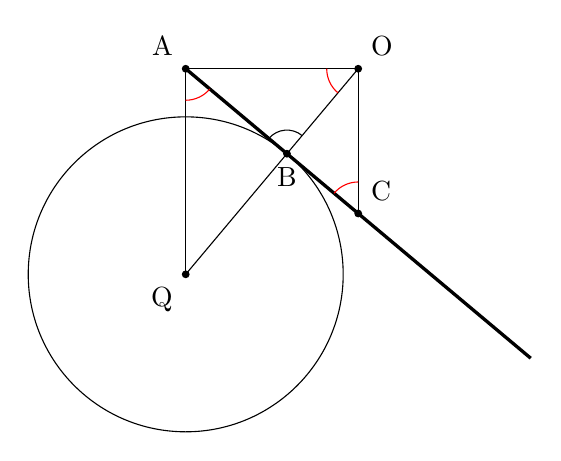
\begin{tikzpicture}
\usetikzlibrary{calc}
\def\angKatus{50};
\def\rKatus{2};
\coordinate (P1) at (0,{\rKatus/sin(\angKatus)});
\coordinate (P2) at ({\rKatus/sin(\angKatus)/tan(\angKatus)},{\rKatus/sin(\angKatus)});
\coordinate (P3) at ({\rKatus/sin(\angKatus)/tan(\angKatus)},{\rKatus/sin(\angKatus)-\rKatus/sin(\angKatus)/tan(\angKatus)/tan(\angKatus)});
%\fill (0,0) circle (0.05);
\node [label=below left:Q, fill=black, circle,inner sep=1pt] at (0,0){};
\draw (0,0) circle (\rKatus);
\node [label=above left:A, fill=black, circle,inner sep=1pt] at (P1){};
\node [label=above right:O, fill=black, circle,inner sep=1pt] at (P2){};
\node [label=above right:C, fill=black, circle,inner sep=1pt] at (P3){};
\node [label=below:B, fill=black, circle,inner sep=1pt] at (\angKatus:\rKatus){};
\draw [very thick](P1) -- (P3) -- ++($(P3)-(P1)$);
\draw (0,0) -- (P2);
\draw (0,0) -- (P1);
\draw (P1) -- (P2);
\draw (P3) -- (P2);
\draw [red](P1) ++ (-90:0.4) arc (-90:-90+\angKatus:0.4);
\draw [red](P3) ++ (90:0.4) arc (90:90+\angKatus:0.4);
\draw [red](P2) ++ (180:0.4) arc (180:180+\angKatus:0.4);
\draw (\angKatus:\rKatus) ++ (\angKatus:0.3) arc (\angKatus:90+\angKatus:0.3);
\end{tikzpicture}
\end{center}

Stabiilsuse analüüsi juures paneme tähele, et kui \enquote{katus} pöörleb tervikuna, siis massikese liigub mööda ringjoont ning küsimus on vaid selles, kas see on kõrgemal või madalamal kui silindri telg $Q$; viimasel juhul on massikese algasendis madalaimas positsioonis ning süsteem on stabiilne. Seega on stabiilsuse tingimuseks
$$|AQ|<|AC|\cos(\alpha/2).$$
Kui sellesse võrratusse asendame
$$|AQ|=|AB|/\cos(\alpha/2)=(L/2)\sin^2(\alpha/2)/\cos(\alpha/2)$$
ja $$|AC|\cos(\alpha/2)=(L/2)\cos(\alpha/2),$$ siis
saame, et $\sin^2(\alpha/2) < \cos^2(\alpha/2)$. Kuna katuse korral peab kehtima $0<\frac{\alpha}{2}<90$, siis nii $\sin$ kui $\cos$ on positiivsed ja võime võtta mõlemalt poolt ruutjuure. Saame tingimuse $\sin(\alpha/2) < \cos(\alpha/2)$, mis kehtib kui $\alpha<\pi/2$. Paneme tähele, et viimast tingimust võib esitada erinevatel viisidel, kasutades $R$, $L$ ja $\alpha$ vahelist seost.
\fi
}

% L314
\ylDisplay{Platvorm} % Ülesande nimi
{Jaan Kalda} % Autor
{lõppvoor} % Voor
{2005} % Aasta
{G 10} % Ülesande nr.
{10} % Raskustase
{
% Teema: Staatika

\ifSolution
\osa Kolmnurk hakkab põranda suhtes liikuma, sest summaarne jõumoment punkti $C$ suhtes koosneb kahest liidetavast, mis omavad ühte ja sama märki ning on nullist erinevad. Selles veendumiseks tuleb tõmmata punktidesse $A$ ja $B$ rakendatud hõõrdejõudude pikendused $AE$ ja $BE$ ($E$ on nende pikenduste lõikepunkt), mis on risti vastavalt raadiustega $OA$ ja $OB$ (vt joonist).\\
\osa Süsteemile mõjub kolm horisontaalsuunalist jõudu. Jõumomentide tasakaalu tingimusest järeldub et nende jõudude pikendused peavad lõikuma ühes punktis $E$. Olgu kolmas keha punktis $D$. Siis punkti $D$ rakendatud hõõrdejõud peab olema suunatud piki sirget $ED$. Teisest küljest, jõudude tasakaalu tingimusest lähtuvalt peavad hõõrdejõudude vektorid moodustama võrdhaarse kolmnurga $\vec F_A+\vec F_B+\vec F_C = 0$ (võrdhaarse, sest punktidesse $A$ ja $B$ rakendatud jõud on moodulilt võrdsed, |$\vec F_A| = |\vec F_B|$).

\begin{center}
	\includegraphics[width=0.7\linewidth]{2005-v3g-10-lah}
\end{center}

Selletõttu peab vektorite $\vec F_A$ ja $\vec F_D$ vaheline nurk võrduma vektorite $\vec F_D$ ja $\vec F_B$ vahelise nurgaga. Niisiis peab sirge $ED$ ristuma nurga $\angle AEB$ poolitajaga $EG$. See tähendab, et punktihulgaks $X$ on sirge $s$, mis ristub nurga $\angle AEB$ poolitajaga $EG$. Lõpetuseks paneme tähele, et hõõrdejõud $\vec F_D$ peab olema moodulilt väiksem, kui $\vec F_A$ ja $\vec F_B$, sest muidu toimuks kolmanda keha juures libisemine. Nii ka on, sest nurk $\angle AEB$ on väiksem kui \SI{60}{\degree} (\SI{60}{\degree}, st võrdkülgse kolmnurga puhul oleks jõudude kolmurgas $\vec F_A + \vec F_B + \vec F_C = 0$ kõik küljed võrdsed, \SI{60}{\degree} väiksemate nurkade puhul aga oleks vektor $\vec F_C$ oma moodulilt teistest väiksem).
\fi
}

% L315
\ylDisplay{Niidiga hantel} % Ülesande nimi
{Jaan Kalda} % Autor
{lõppvoor} % Voor
{2015} % Aasta
{G 9} % Ülesande nr.
{10} % Raskustase
{
% Teema: Staatika

\ifSolution
Pulgale mõjuvad kolm jõudu. Jõumomentide tasakaalu tõttu peavad nende jõudude rakendussirged lõikuma ühes punktis, olgu see punkt $C$. Olgu niidi rakenduspunkt $N$ ja pulga otspunktid $A$ ning $B$, vt joonis. Kuna enne klotsi $A$ paigalt nihkumist pöörleb pulk ümber selle, siis punkti $B$ kiirusvektor on risti $AB$-ga, sama kehtib puntki $B$ rakendatud hõõrdejõu vektori jaoks; sestap $\angle ABC=\frac{\pi}{2}$. Et nihkuma hakkamise hetkel on hõõrdejõud võrdsed, siis jõudude kolmnurk $\vec F_1+\vec F_2=\vec T$ on võrdhaarne, järelikult on võrdhaarne ka jõudude kolmnurgaga sarnane kolmnurk $CBE$ (sirge $BE$ on tõmmatud paralleelsena $\vec T$-ga ja $E$ asub $\vec F_1$ rakendussirgel, vt joonis).
Olgu $|CB|=b$; siis ka $|CE|=b$. Seetõttu kolmnurkade $ANC$ ja $ABE$ sarnasuse põhjal $|AC|=3b$. Pythagorase
teoreemist kolmnurga $ABC$ jaoks $9b^2=b^2+16a^2$, st $b=\sqrt 2a$. Seetõttu otsitav nurk 
\[
\angle BNC=\arctan \frac ba =\arctan \sqrt 2\approx\SI{0.96}{rad}\approx 55^\circ.
\]
\begin{center}
\includegraphics[width=0.7\textwidth]{2015-v3g-09-pulk_lah}
\end{center}
\fi
}

% L316
\ylDisplay{Satelliit} % Ülesande nimi
{Mihkel Pajusalu} % Autor
{piirkonnavoor} % Voor
{2011} % Aasta
{G 2} % Ülesande nr.
{1} % Raskustase
{
% Teema: Taevamehaanika

\ifSolution
\begin{center}
	\includegraphics[width=0.9\linewidth]{2011-v2g-02-lah}
\end{center}
Ringikujulisel orbiidil on satelliidi kiirus kogu orbitaalperioodi jooksul konstantne ja seetõttu on varjus veedetud osa ajast võrdne orbiidi varjus oleva osa pikkuse ja kogu orbiidi pikkuse suhtega, mis on ülal toodud jooniselt leitav kui 
\[
k=\frac{2 \alpha r}{2 \pi r}=\frac{\arcsin \left(\frac{R}{r}\right)}{\pi}=\SI{36,5}{\%}
\]
\fi
}

% L317
\ylDisplay{Väike prints} % Ülesande nimi
{Urmo Visk} % Autor
{piirkonnavoor} % Voor
{2009} % Aasta
{G 1} % Ülesande nr.
{2} % Raskustase
{
% Teema: Taevamehaanika

\ifSolution
Kui väike prints kõnnib piki asteroidi ekvaatorit, mõjub talle gravitatsioonijõud,
mis põhjustab kesktõmbekiirendust. Kaalugu väike prints $m$ kilogrammi. Newtoni
II seaduse põhjal
\[
m \frac{v^{2}}{R}=G \frac{m M}{R^{2}} \quad \Rightarrow \quad v^{2}=\frac{G M}{R}.
\]
Asteroidi mass pole teada, kuid teada on asteroidi tihedus. Kui asteroidi raadius on $R$, siis on asteroidi ruumala $V=\frac{4}{3} \pi R^{3}$ ja mass
\[
M=\rho V=\frac{4}{3} \pi \rho R^{3}.
\]
Asendades massi esialgsesse avaldisse saame
\[
v^{2}=\frac{G M}{R}=\frac{G}{R} \cdot \frac{4}{3} \pi \rho R^{3}=\frac{4}{3} \pi \rho G R^{2}.
\]
Siit avaldame asteroidi raadiuse:
\[
R=v \sqrt{\frac{3}{4 \pi \rho G}}=\frac{v}{2} \sqrt{\frac{3}{\pi \rho G}}=\SI{5}{km}.
\]
\fi
}

% L318
\ylDisplay{Maa pöörlemisperiood} % Ülesande nimi
{Eero Vaher} % Autor
{piirkonnavoor} % Voor
{2014} % Aasta
{G 3} % Ülesande nr.
{2} % Raskustase
{
% Teema: Taevamehaanika

\ifSolution
Päikese näivat liikumist taevas põhjustavad nii Maa pöörlemine kui ka tiirlemine. Maa tiirlemise tõttu erineb Maa täispöörete arv aastas ühe võrra keskmiste päikeseööpäevade arvust. Kuna Maa tiirlemise suund ühtib Maa pöörlemise suunaga, teeb Maa ühe aasta jooksul ühe täispöörde rohkem. Seega on Maa pöörlemisperioodiks
\[
P=\frac{\num{365,256}}{\num{366,256}} \cdot \SI{86400}{\second}=\SI{86164}{\second}=\SI{23}{\hour} \SI{56}{\minute} \SI{4}{\second}.
\]

\vspace{0.5\baselineskip}
\emph{Alternatiivne lahendus}\\
Päike teeb täistiiru taevas sagedusega $f_k=\frac{1}{\SI{86400}{\second}}$. Maa tiirlemise sagedus on $f_t=\frac{1}{\num{365,256}\cdot86400\text{s}}$. Kuna Maa pöörlemis- ja tiirlemissuunad ühtivad, siis kehtib võrrand $f_k=f_p-f_t$, kus $f_p$ on Maa pöörlemise sagedus. Siit saame avaldada Maa pöörlemisperioodi 
\[
P=\frac{1}{f_p}=\frac{1}{f_k+f_t}=\SI{86164}{\second}=\SI{23}{\hour} \SI{56}{\minute} \SI{4}{\second}.
\]

\emph{Märkused.}

\vspace{-5pt}
\begin{itemize}[noitemsep, leftmargin=*]
\item Nimetuse keskmine päikeseööpäev tingib asjaolu, et Maa elliptilise orbiidi tõttu on Päikese näiv nurkkiirus taevas veidi muutlik.
\item Maa tiirlemisperioodi nimetatakse ka sideeriliseks aastaks. 
\item Enamasti mõistetakse aastana troopilist, mitte sideerilist aastat, mis on defineeritud pööripäevade kordumise põhjal. Troopilise ning sideerilise aasta erinemise põhjustab Maa telje pretsessioon. Igapäevaelus ei ole olulised mitte Maa pöörlemine ning tiirlemine vaid hoopis Päikese ööpäevane liikumine taevas ning aastaaegade kordumine, mistõttu laialdaselt kasutatavad ööpäeva ning aasta mõisted erinevadki Maa pöörlemis- ning tiirlemisperioodidest. 
\end{itemize}
\fi
}

% L319
\ylDisplay{Eksinud satelliit} % Ülesande nimi
{Tundmatu autor} % Autor
{lahtine} % Voor
{2009} % Aasta
{G 5} % Ülesande nr.
{3} % Raskustase
{
% Teema: Taevamehaanika

\ifSolution
Leiame geostatsionaarse orbiidi raadiuse, olgu see $r$. Sellel orbiidil on satelliidi tiirlemise periood $T = \SI{24}{h} = \SI{86400}{s}$ ning nurkkiirus $\omega=\frac{2 \pi}{T}=\SI{7,27e-5}{s^{-1}}$. Olgu satelliidi mass $m$ ja Maa mass $M$. Satelliit liigub kekstõmbekiirendusega $a = \omega^2 r$ ning talle mõjub gravitatsioonijõud
\[
F_{G}=G \frac{M m}{r^{2}}.
\]
Newtoni II seaduse põhjal
\[
G \frac{M m}{r^{2}}=m \omega^{2}(R+h) \Rightarrow r^{3}=\frac{G M}{\omega^{2}}.
\]
Raskuskiirendus maapinnal võrdub $g=G \frac{M}{R^{2}}$, kust saame avaldada $GM = gR^2$.
Saame nüüd asendada 
\[
r^{3}=\frac{g R^{2}}{\omega^{2}} \Rightarrow r=\sqrt[3]{\frac{g R^{2}}{\omega^{2}}} \approx \SI{42300}{km}.
\]
Satelliidi orbitaalliikumise kiirus on seega $v_0 = \omega r = \SI{3,08}{km/s}$. Põrkekiirus on maksimaalne siis, kui \enquote{eksinud} satelliit tiirleb samal ringorbiidil mis teised sidesatelliidid, kuid liikumise suund on vastupidine. Sel juhul
\[
v=2 v_{0}=\SI{6,16}{km/s}.
\]
\fi
}

% L320
\ylDisplay{Orbiit} % Ülesande nimi
{Mihkel Pajusalu} % Autor
{lahtine} % Voor
{2014} % Aasta
{G 3} % Ülesande nr.
{3} % Raskustase
{
% Teema: Taevamehaanika

\ifSolution
Selles ülesandes kasutame lähendust, et väikese massiga (olgu selleks $m$) punktmass Kuu tiirleb ümber suure punktmassi Maa. Paneme tähele, et Kuu gravitatsioonilise potentsiaalse energia ja kineetilise energia summa on jääv.
$$
\frac{mv_1^2}{2}-G\frac{Mm}{r_1}=\frac{mv_2^2}{2}-G\frac{Mm}{r_2}.
$$
Samuti on kõigil orbiitidel liikuvatel kehadel muutumatu impulsimoment. Kuna orbiidid on ellipsid, siis suurimal ja vähimal kaugusel Maast on Kuu orbitaalkiirus risti Kuud Maaga ühendava sirgega. Seega saab kirjutada impulsimomendi jäävuse seaduse suurima ja vähima kauguse jaoks kujul
$$
mv_1r_1=mv_2r_2.
$$
Kuu mass taandub mõlemast jäävusseadusest välja. Saame süsteemi
$$
\begin{array}{c} 
\frac{v_1^2}{2}-G\frac{M}{r_1}=\frac{v_2^2}{2}-G\frac{M}{r_2}.\\
v_1r_1=v_2r_2.
\end{array}
$$
Süsteemi lahenditeks on $r_2=r_1$, mis ei vasta elliptilisele orbiidile, ja $$r_2=\frac{1}{\frac{2GM}{r_1^2v_1^2}-\frac{1}{r_1}}\approx\SI{430000}{km}.$$
\fi
}

% L321
\ylDisplay{Päikese tihedus} % Ülesande nimi
{Eero Vaher} % Autor
{piirkonnavoor} % Voor
{2013} % Aasta
{G 6} % Ülesande nr.
{4} % Raskustase
{
% Teema: Taevamehaanika

\ifSolution
Päikese raadius on $r=R\sin\alpha/2$ ja ruumala $V=4\pi r^3/3$.
Maa joonkiirus oma orbiidil ümber Päikese on $v=\frac{2\pi R}{T}$. Et Maa püsiks oma orbiidil, peab sellele mõjuma kesktõmbejõud $F=\frac{mv^2}{R}$, kus $m$ on Maa mass. See kesktõmbejõud on teadagi Maa ja Päikese vaheline gravitatsioonijõud $G\frac{mM}{R^2}$, kus $M$ on Päikese mass, seega
\[
\frac{mv^2}{R}=G\frac{mM}{R^2}.
\]
Saame
\[
M=\frac{Rv^2}{G}.
\]
Päikese tihedus avaldub seosest $\varrho=\frac{M}{V}$, $$\varrho=\frac{Rv^2}{G} \frac{3}{4\pi r^3}=\frac{24 \pi R^3}{G T^2 \sin^3 \alpha}=\SI{1,4e3}{kg/m^3}.$$
\fi
}

% L322
\ylDisplay{Ühendatud satelliidid} % Ülesande nimi
{Eero Vaher} % Autor
{piirkonnavoor} % Voor
{2018} % Aasta
{G 6} % Ülesande nr.
{4} % Raskustase
{
% Teema: Taevamehaanika

\ifSolution
Trossi puudumisel peab satelliidile mõjuv kesktõmbejõud olema võrdne sellele mõjuva raskusjõuga. Esimese satelliidi jaoks
\[
\frac{{mv'_1}^2}{R_1}=G\frac{Mm}{R_1^2},
\]
millest järeldub
\[
v'_1=\sqrt{\frac{GM}{R_1}}
\]
ning analoogiliselt
\[
v'_2=\sqrt{\frac{GM}{R_2}}.
\]

Kuna satelliidid on trossiga ühendatud, siis seesmisele satelliidile mõjuv kesktõmbejõud peab olema sellele mõjuva raskusjõu ning trossi pinge vahe ning välimisele satelliidile mõjuv kesktõmbejõud peab olema sellele mõjuva raskusjõu ning trossi pinge summa. Niisiis
$$\begin{cases}
\frac{mv_1^2}{R_1}=G\frac{Mm}{R_1^2}-T,\\
\frac{mv_2^2}{R_2}=G\frac{Mm}{R_2^2}+T.
\end{cases}$$ 
Kuna $v_1=2\pi R_1/P$ ning $v_2=2\pi R_2/P$, siis saame kirjutada
$$\frac{4\pi^2}{P^2}\left(R_1+R_2\right)=GM\frac{R_2^2+R_1^2}{R_1^2R_2^2}.$$
Tehes asenduse $R_2=2R_1$, saame
\[
\frac{2\pi R_1}{P}=\sqrt{\frac{5GM}{12R_1}},
\]
ning asendusest $R_1=\frac{R_2}{2}$ järeldub
\[
\frac{2\pi R_2}{P}=\sqrt{\frac{10GM}{3R_2}}.
\]
Sisemine satelliit tiirleb niisiis trossi tõttu $\sqrt{12/5}$ korda väiksema ning välimine $\sqrt{10/3}$ korda suurema joonkiirusega.
\fi
}

% L323
\ylDisplay{Satelliit} % Ülesande nimi
{Eero Vaher} % Autor
{lõppvoor} % Voor
{2013} % Aasta
{G 5} % Ülesande nr.
{5} % Raskustase
{
% Teema: Taevamehaanika

\ifSolution
Satelliidile orbiidil mõjuv kesktõmbejõud on Maa poolt satelliidile avaldatav gravitatsioonijõud. Saame $$\frac{mv^2}{R}=G\frac{Mm}{R^2},$$kus $m$ on satelliidi mass ja $R$ orbiidi raadius. Kuna geostatsionaarne satelliit Maa suhtes ei liigu, peab selle tiirlemisperiood olema samuti 24 h. Saame $v=\frac{2\pi R}{t}$. Neist võrranditest saame $$4\pi^2 R^3=GM \Rightarrow R=\sqrt[3]{\frac{GMt^2}{4\pi^2}}=\SI{42400}{km}.$$ Maa keskpunkt, satelliit ning satelliidilt nähtava maa-ala serval asetsev suvaline punkt moodustavad täisnurkse kolmnurga, mille hüpotenuusiks on satelliidi orbiidi raadius ning üheks kaatetiks Maa raadius. Maa keskmes asuvaks nurgaks saame $\alpha=\arccos{\frac{r}{R}}$, kuid kuna meid huvitab satelliidilt nähtava ala läbimõõt, peame leidma nurga $2\alpha$. Sellele nurgale vastav kaare pikkus Maa pinnal on $d=2r\alpha$ (kui nurk on radiaanides). Lõppvastuseks saame 
$$d=2r\arccos \left(\frac{r}{\sqrt[3]{\frac{GMt^2}{4\pi^2}}}\right) =\SI{18000}{km}.$$
\fi
}

% L324
\ylDisplay{Kosmosejaam} % Ülesande nimi
{Oleg Košik} % Autor
{lõppvoor} % Voor
{2005} % Aasta
{G 9} % Ülesande nr.
{6} % Raskustase
{
% Teema: Taevamehaanika

\ifSolution
Maa pöörlemise tõttu ümber oma telje tekivad trajektoori nihked. Mõõdame nihke pikkuse ekvaatoril $\Delta l$ ning ekvaatori pikkuse (ehk kogu kaardi laiuse) $l$. Nende suhe määrab kosmosejaama nurkkiiruse $\omega_J$ ja maa pöörlemise nurkkiiruse $\omega_M$ suhte:
\[
\alpha=\frac{l}{\Delta l}=\frac{\omega_{J}}{\omega_{M}} \approx \num{15,7}.
\]
Arvestades, et maa pöörlemise nurkkiirus on $\omega_M = 2\pi /T$, kus $T$ on ööpäeva pikkus ehk \SI{86400}{s}, leiame
\[
\omega_J = \alpha \omega_M = \frac{2\pi\alpha}{T}.
\]
Kosmosejaamale mõjuv gravitatsioonijõud määrab kesktõmbekiirenduse:
\[
m g^{\prime}= m\omega_J^2 r = m \omega_{J}^{2}(R+h),
\]
kus $g'$ on raskuskiirendus kõrgusel $h$ maapinnast. Gravitatsiooniseadusest teame, et raskuskiirendus on pöördvõrdeline kauguse ruuduga, millest
\[
g^{\prime}= g\left(\frac{R}{r}\right)^2 = g\left(\frac{R}{R+h}\right)^{2}.
\]
Kombineerides kaks viimast võrrandit, saame
\[
\omega_{J}^{2}(R+h)=g\left(\frac{R}{R+h}\right)^{2},
\]
kust ostitav kõrgus on
\[
h=\sqrt[3]{\frac{g R^{2}}{\omega_{J}^{2}}}-R=\sqrt[3]{\frac{g R^{2} T^{2}}{4 \pi^{2} \alpha^{2}}}-R \approx \SI{359}{km}.
\]

\emph{Märkus}. Tegelik kõrgus varieerub \num{350} ja \SI{365}{km} vahel (Maa raadius ei ole kõikjal ühesugune). Siin $\alpha$ väärtus oli mõõdetud suhteliselt täpsete arvutigraafika vahenditega, joonlauga joonise mõõtmise korral esinevate ebatäpsuste tõttu võib vastus erineda tegelikust kuni \num{200} kilomeetri võrra. 
\fi
}

% L325
\ylDisplay{Kuukaabel} % Ülesande nimi
{Siim Ainsaar} % Autor
{piirkonnavoor} % Voor
{2009} % Aasta
{G 10} % Ülesande nr.
{8} % Raskustase
{
% Teema: Taevamehaanika

\ifSolution
\osa
Maa avaldab kaablile jõudu
\[ 
F_M = G m_M \lambda \left( \frac{1}{r_M} - \frac{1}{D - r_K} \right),
\]
analoogiliselt Kuu,
\[ 
F_K = G m_K \lambda \left( \frac{1}{r_K} - \frac{1}{D - r_M} \right).
\]
Suhe on seega
\[ \frac{F_M}{F_K} = \frac{ m_M \left( \frac{1}{r_M} - \frac{1}{D -
		r_K} \right) }{ m_K \left( \frac{1}{r_K} - \frac{1}{D - r_M} \right) } \approx
\num{21,9}.\]

\osa
Leiame kaablit pingutava jõu $T(x)$ Kuu keskmest mingil kaugusel $x$. Sellest
kaugusest Maa-poolset kaabliosa mõjutavad kolm jõudu: kaabli pinge $T(x)$ ning
Maa ja Kuu poolt avaldatavad raskusjõud. ($x$-st Kuu-poolset osa mõjutab ka
otsa Kuu küljes hoidev jõud, selle arvutamiseks pole tarvidust.) Nimetatud jõud on
tasakaalus, mistõttu
\[ 
T(x) = G\lambda m_M \left( \frac{1}{r_M} - \frac{1}{D-x} \right) -
G\lambda m_K \left( \frac{1}{x} - \frac{1}{D-r_M} \right) \text. 
\]

Kaabel katkeks sealt, kus pinge on tugevaim, seega lahendame
ekst\-ree\-mum\-üles\-an\-de
ja leiame $T(x)$ maksimumi. Seal tuletis $T'(x)=0$. Kui saame ainult ühe mõistliku lahendi, pole
ekstreemumi liigi määramiseks teist tuletist vajagi: teame, et kosmoses on $T$
suurem kui kaabli otstes (taevakehapinnalt kaabliosade eralduspunkti
eemaldades kasvab lähema keha tõmme alumisele, \enquote{tekkivale} kaablipoolele ilmselt kiiremini
kui kahaneb teise keha tõmme ülemisele; osade suhtelised massid muutuvad
oluliselt erineva kiirusega), tänu millele (vähemalt) üks maksimum eksisteerib.
\[ 
T'(x) = - \frac{ G\lambda m_M }{ (D-x)^2 } + \frac{ G\lambda m_K }{ x^2 } = 0
\implies x = \frac{D}{1 \pm \sqrt{\frac{m_M}{m_K}}}.
\]
Miinusmärgiga lahend on negatiivsena mittefüüsikaline, seega otsitavaks
kõr\-gu\-seks osutub
\[ 
h = \frac{D}{1 + \sqrt{\frac{m_M}{m_K}}} - r_K \approx
\SI{36200}{km}.
\]
\fi
}

% L326
\ylDisplay{Satelliidid} % Ülesande nimi
{Mihkel Kree} % Autor
{lõppvoor} % Voor
{2010} % Aasta
{G 7} % Ülesande nr.
{9} % Raskustase
{
% Teema: Taevamehaanika

\ifSolution
Lähtume analoogiast molekulaarfüüsikaga, kus ühe molekuli vaba tee hindamisel arvestatakse, et molekul liigub ilma põrgeteta tüüpiliselt aja jooksul, mil tema kokkupõrke-ristlõige on katnud ruumala, milles asub tüüpiliselt üks osake (see ruumala avaldub kui anuma ruumala jagatud osakeste arvuga). Kokkupõrke-ristlõige pole päris identne osakese enda ristlõikega -- vaatleme näiteks kera-kujulisi osakesi raadiusega $r$, osakesed põrkuvad kui nende tsentrid ei ole teineteisest kaugemal kui $2r$, niisiis on ühe osakese kokkupõrke-ristlõige neli korda suurem tema ristlõikest.

Satelliidid liiguvad ruumiosas ruumalaga
\[ V=\frac{4\pi}{3}\left[(R+h_2)^3-(R+h_1)^3\right]\approx \SI{1.2e12}{km^3}.\]
Liikumisruum ühe satelliidi kohta on seega $V/N$ (niisuguse ruumalaga suvaliselt valitud ruumiosast leiame tüüpiliselt ühe satelliidi).

Aja $t$ jooksul katab ühe satelliidi kokkupõrke-ristlõige ruumala
\[V_t=4Svt,\]
kus $v$ on tüüpiline satelliidi liikumise kiirus. Me ei tee suurt viga, võttes $v$ väärtuseks esimese kosmilise kiiruse (kiirus sõltub raadiuse ruutjuurest ning suhteline viga oleks ainult \mbox{$\sqrt{\frac{6400+2000}{6400}}\approx\num{1.15}$}):
\[\frac{v^2}{R}=\frac{GM}{R^2}=g.\]
Niisiis,
\[V_t=\sqrt{gR}4St.\]

Eelneva arutluse kohaselt arvestame, et ühel satelliidil tuleb kokkupõrget oodata niisugune ajavahemik $t$, et $V_t=V/N$. Et meil on aga $N$ satelliiti, siis esimese niisuguse kokkupõrkeni kulub $N$ korda vähem aega. Seega,
\[
\Delta t=\frac{V}{N^24S\sqrt{gR}}=\frac{\num{1.2e12}\cdot 10^9}{\num{4}\cdot\num{2.5}^2\cdot 10^6\cdot \num{10}\cdot \sqrt{10 \cdot \num{64} \cdot 10^2\cdot 10^3}}s=\SI{6e8}{s},
\]
ehk
\[
\Delta t=\frac{6\cdot10^{8}}{3600\cdot24\cdot365}\approx \SI{19}{a}.
\]
\fi
}

% L327
\ylDisplay{Balloon} % Ülesande nimi
{Jaan Susi} % Autor
{lõppvoor} % Voor
{2005} % Aasta
{G 3} % Ülesande nr.
{1} % Raskustase
{
% Teema: Termodünaamika

\ifSolution
Termodünaamika I seaduse kohaselt $\Delta U = Q - A$, kus $Q$ on süsteemi antud soojushulk ning $A$ on välisjõudude vastu tehtud töö. Antud ülesande kontekstis on $Q$ negatiivne ja $A$ positiivne ning $A = p\Delta V$ ja $Q = -\lambda \rho_vV$. Niisiis,
\[
\Delta U=-\lambda \rho_{v} V-p\left(\frac{V \rho_{v}}{\rho_{j}}-V\right)=-\rho_{v} V\left[\lambda+p\left(\rho_{j}^{-1}-\rho_{v}^{-1}\right)\right].
\]
Paneme tähele, et avaldis nurksulgudes peaks kujutama endast sulamissoojust normaaltingimustel (sest vee võib viia samasse lõppolekusse ka teisel viisil --- muutes ta jääks normaaltingimustel ning seejärel viies rõhu etteantud väärtuseni; et jää loeme kokkusurumatuks, siis rõhu tõstmisel tööd ei tehta). Paistab, et tegemist pole siiski päris hariliku veega, sest
\[
\lambda+p\left(\rho_{j}^{-1}-\rho_{v}^{-1}\right)= \SI{323}{kJ/kg} \neq \lambda_{0}=\SI{334}{kJ/kg}.
\]
Arvandmete asendamisel leiame $\Delta U = \SI{-3,23}{MJ}$.
\fi
}

% L328
\ylDisplay{Kütteklaas} % Ülesande nimi
{Jaak Kikas} % Autor
{lõppvoor} % Voor
{2007} % Aasta
{G 1} % Ülesande nr.
{1} % Raskustase
{
% Teema: Termodünaamika

\ifSolution
Kehtivad valemid
\[
P=\frac{U^{2}}{R}, \quad R=\frac{\rho L}{S},
\]
kus $\rho$ on kattekihi eritakistus. Seega vastavalt orientatsioonile $R_H = \rho b/da$ ja $R_V = \rho a/db$, kus $d$ on kattekihi paksus. Niisiis,
\[
P_H/P_V = a ^2/b^2 = \num{0,25}.
\]

\fi
}

% L329
\ylDisplay{Jääkuul} % Ülesande nimi
{Urmo Visk} % Autor
{piirkonnavoor} % Voor
{2008} % Aasta
{G 4} % Ülesande nr.
{1} % Raskustase
{
% Teema: Termodünaamika

\ifSolution
Rõhk kuuli sees kasvab seetõttu, et õhk kuulis soojeneb. Ülesande teksti põhjal võime eeldada, et õhu temperatuur kuuli sees on võrdne tema seinte temperatuuriga. Meie ülesandeks on kontrollida, kui palju on rõhk kasvanud selleks hetkeks, kui seinad hakkavad sulama, st on saavutanud temperatuuri $t_1 = \SI{0}{\celsius}$. 

Eeldame, et kera soojuspaisumine on tühine. Siis on õhu ruumala keras konstantne. Isohoorilises protsessis kehtib seos 
\[
\frac{p_1}{T_1} = \frac{p_0}{T_0}.
\]
Tähistame indeksiga \enquote{0} gaasi omadusi külmikus ja indeksiga \enquote{1} omadusi temperatuuril, mille juures seinad hakkavad sulama. Niisiis 
\[
p_1 = p_0 \frac{T_1}{T_0}.
\] 
Kasutades seda tulemust saame avaldada rõhu suhtelise muutuse 
\[
\frac{\Delta p}{p_{0}}=\frac{p_{1}-p_{0}}{p_{0}}=\left(\frac{T_{1}}{T_{0}}-1\right).
\]
Leiame selle avaldise numbrilise väärtuse: 
\[
\frac{\Delta p}{p_0} \approx \num{0,034} = \SI{3,4}{\%}.
\] 
See on selgelt väiksem, kui kuuli seinte purunemispiir, st kuul hakkab enne sulama (kuid puruneb ilmselt ülerõhu tõttu enne lõplikku ära sulamist). 

\emph{Märkus}. Alternatiivse ja võrdväärse lahendusena võib leida, millise õhutemperatuuri juures saavutaks suhteline ülerõhk väärtuse \SI{20}{\%} (selleks tuleb \SI{317}{K} ehk \SI{44}{\celsius}) ja võrrelda seda jää sulamistemperatuuriga.
\fi
}

% L330
\ylDisplay{Küttesüsteem} % Ülesande nimi
{Tundmatu autor} % Autor
{piirkonnavoor} % Voor
{2011} % Aasta
{G 3} % Ülesande nr.
{1} % Raskustase
{
% Teema: Termodünaamika

\ifSolution
Paisumisel lisanduva ruumala jaoks peab olema paisupaagis piisavalt lisaruumi. Vajalik ruumala on
\[
V-V_{1}=V_{0}\left(1+\beta t_{2}\right)-V_{0}\left(1+\beta t_{1}\right)=\frac{V_{1} \beta}{1+\beta t_{1}}\left(t_{2}-t_{1}\right).
\]
Vajalik vaba ruum paisupaagis on seega $V - V_1 \approx \SI{4,0}{l}$.
\fi
}

% L331
\ylDisplay{Vee jäätumine} % Ülesande nimi
{Jaak Kikas} % Autor
{lahtine} % Voor
{2012} % Aasta
{G 1} % Ülesanne nr.
{1} % Raskustase
{
% Teema: Termodünaamika

\ifSolution
Vee jäätumisel eralduv soojushulk $m\idx{vesi} \lambda$ peab täpselt ära kuluma jää soojendamiseks:
\[
m\idx{vesi} \lambda = c\idx{jää} m\idx{jää} (t - t_0),
\]
kus $\lambda$ on jää sulamissoojus, $t=\SI{0}{\celsius}$ on jää lõpptemperatuur ja $t_0$ on otsitav jää algtemperatuur. Vee massi saame selle ruumalast, $m\idx{vesi} = \rho V\idx{vesi}$. Nendest kahest seosest saame avaldada
$$t_0 = t - \frac{\rho V\idx{vesi} \lambda}{c\idx{jää} m\idx{jää}} = -314 \,^{\circ}{\rm C}.$$
Ehk jää temperatuur peaks olema alla absoluutse nulli ja seega pole võimalik selle koguse jääkuubikutega kogu vett jääks muuta.
\fi
}

% L332
\ylDisplay{Veepudel} % Ülesande nimi
{Koit Timpmann} % Autor
{piirkonnavoor} % Voor
{2013} % Aasta
{G 2} % Ülesande nr.
{1} % Raskustase
{
% Teema: Termodünaamika

\ifSolution
Vesi jäätub temperatuuril \SI{0}{\celsius}. Vee jäätumisel eraldunud soojushulk läheb alajahtunud vee soojendamiseks jäätumistemperatuurile. Niisiis,
\[
cm\Delta t = \lambda m\idx{jää}
\]
ja
\[
m\idx{jää}=\frac{\SI{4200}{J / kg K} \cdot \SI{2}{kg} \cdot \SI{3}{\celsius}}{\SI{340000}{J / kg}}=\SI{74}{g}.
\]
\fi
}

% L333
\ylDisplay{Ringprotsess} % Ülesande nimi
{Riho Taba} % Autor
{piirkonnavoor} % Voor
{2006} % Aasta
{G 2} % Ülesande nr.
{2} % Raskustase
{
% Teema: Termodünaamika

\ifSolution
Antud joonise saab teisendeda telgedega $P$ ja $V$ graafikuks, kus iga tsükli osa töö on arvuliselt võrdne antud graafiku osa alla jääva pindalaga (sest tehtud töö on $P\Delta V$). Ideaalse gaasi töö protsessi osal $1 \rightarrow 2$: $A_{1\rightarrow 2} = 0$, protsessi osal $2 \rightarrow 3$: $A_{2\rightarrow 3} < 0$ ning protsessi osal $3 \rightarrow 1$: $A_{3\rightarrow 1} > 0$, kuid $|A_2\rightarrow 3| > |A_3\rightarrow 1|$, seega $A_{1\rightarrow 2\rightarrow 3} < 0$, ehk gaasi tehtud töö on negatiivne.

\begin{center}
	\includegraphics[width=0.4\linewidth]{2006-v2g-02-lah}
\end{center}
\fi
}

% L334
\ylDisplay{Vedelike segamine} % Ülesande nimi
{Aleksei Vlassov} % Autor
{piirkonnavoor} % Voor
{2007} % Aasta
{G 3} % Ülesande nr.
{2} % Raskustase
{
% Teema: Termodünaamika

\ifSolution
Olgu vedelike tihedused vastavalt $\rho_1$ ja $\rho_2$ ning erisoojused $c_1$ ja $c_2$. Olgu otsitav temperatuur $t_4$. Paneme kirja energia jäävuse võrrandid mõlema segu jaoks:
\[
\left\{\begin{array}{l}
	{\rho_{1} V c_{1}\left(t_{3}-t_{1}\right)=\rho_{2} V c_{2}\left(t_{2}-t_{3}\right)} \\ {2 \rho_{1} V c_{1}\left(t_{4}-t_{1}\right)=\rho_{2} V c_{2}\left(t_{2}-t_{4}\right)}\end{array} \Rightarrow\left\{\begin{array}{l}{\rho_{1} c_{1}\left(t_{3}-t_{1}\right)=\rho_{2} c_{2}\left(t_{2}-t_{3}\right)} \\ {2 \rho_{1} c_{1}\left(t_{4}-t_{1}\right)=\rho_{2} c_{2}\left(t_{2}-t_{4}\right).}
\end{array}\right.\right.
\]
Korrutame esimese võrrandi vasaku poole läbi teise võrrandi parema poolega:
\[
\rho_{1} c_{1} \rho_{2} c_{2}\left(t_{3}-t_{1}\right)\left(t_{2}-t_{4}\right) =2 \rho_{1} c_{1} \rho_{2} c_{2}\left(t_{4}-t_{1}\right)\left(t_{2}-t_{3}\right).
\]
ehk
\[
\left(t_{3}-t_{1}\right)\left(t_{2}-t_{4}\right) =2\left(t_{4}-t_{1}\right)\left(t_{2}-t_{3}\right).
\]
Siit avaldame $t_4$:
\[
t_{4}=\frac{t_{1} t_{2}+t_{2} t_{3}-2 t_{1} t_{3}}{2 t_{2}-t_{1}-t_{3}}=\SI{39}{\celsius}.
\]
\fi
}

% L335
\ylDisplay{Tulehõõrumine} % Ülesande nimi
{Jaak Kikas} % Autor
{piirkonnavoor} % Voor
{2008} % Aasta
{G 3} % Ülesande nr.
{2} % Raskustase
{
% Teema: Termodünaamika

\ifSolution
Varda pöörlemisel käigus muutub hõõrdejõu ületamiseks tehtud töö soojuseks. Toru otspinna ja aluse vahel mõjub hõõrdejõud $F_h$, mis võrdub pinnaga ristuva rõhumisjõu ja hõõrdeteguri korrutisega. Rõhumisjõuks on jõud $F$, millega surutakse toru vastu alust. Seega $F_h = \mu F$. Kui toru teeb ühe pöörde, siis läbib toru sein teepikkuse $L = \pi D$. Hõõrdejõu ületamiseks tehti ühe pöörde läbimisel töö $A = F_hL$. Kui toru pöörleb sagedusega $f$, siis aja $t$ jooksul teeb toru $N = f t$ pööret. Kokku eraldub toru pöörlemisel soojushulk
\[
Q=A N=\mu F \pi D f \Delta t.
\]
\fi
}

% L336
\ylDisplay{Termos} % Ülesande nimi
{Urmo Visk} % Autor
{piirkonnavoor} % Voor
{2009} % Aasta
{G 3} % Ülesande nr.
{2} % Raskustase
{
% Teema: Termodünaamika

\ifSolution
Olgu $c_x$ otsitav erisoojus.

Vaatleme esimest juhtu, kus termoses oli algselt külmem vesi. Kuna külmem vesi oli termosega soojuslikus tasakaalus, siis oli ka termose temperatuur $t_1$. Temperatuuride
ühtlustumisel annab soojem vesi energiat ära. Külmem vesi ja termos saavad energiat juurde. Paneme kirja soojusliku tasakaalu võrrandi:
\begin{equation}
m_{1} c\left(T_{1}-t_{1}\right)+m c_{x}\left(T_{1}-t_{1}\right)=m_{2} c\left(t_{2}-T_{1}\right).
\label{2009-v2g-03:eq1}
\end{equation}
Vaatleme teist juhtu, kus termoses oli algselt soojem vesi. Kuna soe vesi oli termosega soojuslikus tasakaalus, siis oli ka termose temperatuur $t_2$. Temperatuuride
ühtlustumisel annavad termos ja soojem vesi energiat ära. Külmem vesi saab energiat juurde. Kirjutame soojusliku tasakaalu võrrandi:
\begin{equation}
m_{1} c\left(T_{2}-t_{1}\right)=m_{2} c\left(t_{2}-T_{2}\right)+m c_{x}\left(t_{2}-T_{2}\right).
\label{2009-v2g-03:eq2}
\end{equation}
Lahutame teineteisest võrrandid (\ref{2009-v2g-03:eq2}) ja (\ref{2009-v2g-03:eq1}).
\[
m_{1} c\left(T_{1}-T_{2}\right)+m c_{x}\left(T_{1}-t_{1}\right)=m_{2} c\left(T_{2}-T_{1}\right)-m c_{x}\left(t_{2}-T_{2}\right).
\]
Tähistame $T_2 - T_1 = \Delta T$. Allpool on toodud $c_x$ tuletuskäik eelnevast valemist.
\[
-m_{1} c \Delta T+m c_{x}\left(t_{2}-t_{1}\right)=m_{2} c \Delta T+m c_{x} \Delta T\implies
\]
\[
-\Delta T c\left(m_{2}+m_{1}\right)=m c_{x}\left(\Delta T+t_{1}-t_{2}\right)\implies
\]
\[
c_{x}=-\frac{\Delta T c\left(m_{2}+m_{1}\right)}{m\left(\Delta T+t_{1}-t_{2}\right)}=\SI{930}{J/kg.C}.
\]
\fi
}

% L337
\ylDisplay{Rauatükk} % Ülesande nimi
{Oleg Košik} % Autor
{lahtine} % Voor
{2010} % Aasta
{G 2} % Ülesande nr.
{2} % Raskustase
{
% Teema: Termodünaamika

\ifSolution
Algne vee mass on $M=\rho V=\SI{1000}{g}$. Olgu väljaaurustunud vee mass $m_0$. Selle soojendamiseks keemistemperatuurini $t=\SI{100}{\celsius}$ ning aurustamiseks läheb vaja energiat
\[
Q_1=m_0(c_1(t-t_1)+L).
\]
Ülejäänud vee soojendamiseks temperatuurini $t_2$ läheb energiat
\[
Q_2=(M-m_0)c_1(t_2-t_1).
\]
Raua jahtumisel eraldub energia $Q_3=mc_2(t_0-t_2)$. Energia jäävuse seaduse kohaselt $Q_1+Q_2=Q_3$, ehk
\[
m_0(c_1(t-t_1)+L)+(M-m_0)c_1(t_2-t_1)=mc_2(t_0-t_2).
\]
Siit
\[
m_0=\frac{mc_2(t_0-t_2)-Mc_1(t_2-t_1)}{c_1(t-t_2)+L}\approx \SI{2}{g}.
\]
\fi
}

% L338
\ylDisplay{Jõhvikad} % Ülesande nimi
{Urmo Visk} % Autor
{piirkonnavoor} % Voor
{2010} % Aasta
{G 2} % Ülesande nr.
{2} % Raskustase
{
% Teema: Termodünaamika

\ifSolution
Vee algtemperatuur oli $t_1=\SI{100}{\celsius}$. Olgu vee ja jõhvikate massid vastavalt $M$ ja $m$. Jõhvikate soojendamiseks kuluv soojushulk tuleb vee jahtumise arvelt. Vee jahtumisel eralduv soojushulk oli
\[
Q_j=Mc_V(t_1-t).
\]
Jõhvikate soojendamise käigus tuli 1) soojendada külmunud jõhvikad sulamistemperatuurini, 2) sulatada külmunud jõhvikad ja 3) soojendada sulanud jõhvikad vee temperatuurini.
Leiame igas etapis kulunud soojushulga:
\[
\begin{aligned}
Q_{s1}&=mc_j(0-t_2)=-mc_jt_2,\\
Q_{s2}&=mL,\\
Q_{s3}&=mc_v(t-0)=mc_vt.
\end{aligned}
\]
Liidame jõhvikate soojendamiseks kulunud soojushulgad ja võrdsustame saadud summa vee jahtumisel eraldunud soojushulgaga. Saadud võrrandist avaldame vee ja jõhvikate masside suhte:
\[
-mc_jt_2+mL+mc_vt=Mc_V(t_1-t),
\]
kust
\[
\frac{M}{m}=\frac{-c_jt_2+L+c_vt}{c_V(t_1-t)}.
\]
Arvuliseks vastuseks saame \num{16}.
\fi
}

% L339
\ylDisplay{Vesi} % Ülesande nimi
{Taavi Pungas} % Autor
{lõppvoor} % Voor
{2011} % Aasta
{G 1} % Ülesande nr.
{2} % Raskustase
{
% Teema: Termodünaamika

\ifSolution
Energia jäävusest teame, et väikese koguse vee aurustumiseks kuluv soojushulk tuleb järelejäänud vee temperatuuri langemise arvelt.

Kuigi aurustumise alghetkel tekib veeaur temperatuuriga \SI{100}{\celsius}, on hiljem nii vee
kui tekkiva veeauru temperatuur veidi madalam. Uuel temperatuuril aga ei ole enam
väikese koguse vee aurustumiseks kuluv soojushulk otseselt arvutatav vee aurustumissoojusest temperatuuril \SI{100}{\celsius} (ülesandes antud $L$).

Seega teeme lihtsustuse, et vee aurustumissoojus on selles temperatuurivahemikus kogu aeg $L$. Olgu esialgselt termoses oleva vee mass $m$. Saame $\num{0,01}mL = \num{0,99}mc_v\Delta t$, mis annab vastuseks
\[
\Delta t=\frac{1}{99} \frac{L}{c_{v}}=\SI{5,4}{\celsius}.
\]
\fi
}

% L340
\ylDisplay{Hõõrdkeevitus} % Ülesande nimi
{Ants Remm} % Autor
{lõppvoor} % Voor
{2012} % Aasta
{G 1} % Ülesande nr.
{2} % Raskustase
{
% Teema: Termodünaamika

\ifSolution
Hõõrdumisest tekkiv soojushulk
\[
Q = F_h \Delta s = F \mu \Delta s = \pi f D \Delta t.
\]
Teiselt poolt on torude soojendamiseks vaja minev soojushulk
\[
Q = 2 m c \Delta T = 2 \rho V c \Delta T,
\]
kus $m$ ja $V$ on ühe toruotsa soojeneva osa mass ja ruumala. Kuna toru seinad on diameetrist kordades õhemad, võib hinnata ruumalaks $V = \pi D d l$. Kokkuvõttes saame, et
\[
F \mu \pi f D \Delta t = 2 \pi D d l \rho c ( T_1 - T_0 ),
\]
\[
F = \frac{2 d l \rho c ( T_1 - T_0 )}{ \mu f \Delta t } \approx \SI{1200}{N}.
\]
\fi
}

% L341
\ylDisplay{Münt jääs} % Ülesande nimi
{Erkki Tempel} % Autor
{piirkonnavoor} % Voor
{2015} % Aasta
{G 3} % Ülesande nr.
{2} % Raskustase
{
% Teema: Termodünaamika

\ifSolution
Jäätükk koos mündiga hakkab uppuma siis, kui sellele mõjub raskusjõud on võrdne üleslükkejõuga. Tähistame uppumise hakkamise hetkel mündi ümber oleva jää massi $m$ ning ruumala $V$. Sellisel juhul mõjub jäätükile enne uppuma hakkamist raskusjõus $F_r=(m_m+m)g$ ning üleslükkejõud
\[ F_y=\rho_v g(V + V_m)=\rho_v g\left(\frac{m}{\rho_j} + \frac{m_m}{\rho_m}\right). \]

Kuna raskusjõud ja üleslükkejõud on uppumise hakkamise hetkel võrdsed, saame avaldada mündi ümber olnud jää massi $m$:
\[ m = \frac{\rho_j m_m(\rho_m - \rho_v)}{\rho_m(\rho_v - \rho_j)} = \SI{79,9}{g}. \]
Sulanud jää mass $m_s$ on seega
\[ m_s = m_j - m = m_j - \frac{\rho_j m_m(\rho_m - \rho_v)}{\rho_m(\rho_v - \rho_j)}. \]
Jää sulamiseks vajaminev energia $Q=\lambda m_s$ saadakse vee jahtumisel eraldunud energiast $Q=cm_v\Delta T$. Võrdsustades viimased avaldised ning avaldades $\Delta T$, saame
\[ \Delta T = \frac{\lambda m_s}{cm_v}. \]
Asendades siia sulanud jää massi $m_s$, saame temperatuuri muutuseks
\[ \Delta T \approx \SI{9,8}{\celsius}. \]
Kuna vee lõpptemperatuur pärast soojusvahetuse lakkamist on \SI{0}{\celsius}, peab vee algtemperatuur olema \SI{9,8}{\celsius}.
\fi
}

% L342
\ylDisplay{Soojusvaheti} % Ülesande nimi
{Kaur Aare Saar} % Autor
{lõppvoor} % Voor
{2016} % Aasta
{G 1} % Ülesande nr.
{2} % Raskustase
{
% Teema: Termodünaamika

\ifSolution
Nafta jahtumisel eraldunud soojus kulub vee soojendamiseks: $Q\idx{nafta} = Q\idx{vesi},$
\[ m_nc_n\Delta t_n = m_vc_v\Delta t_v \quad\Rightarrow \]
\[ \rho_nv_nc_n\Delta t_n = \rho_v v_vc_v\Delta t_v \quad\Rightarrow\quad \Delta t_v = \frac{\rho_nv_nc_n\Delta t_n}{\rho_vv_vc_v} \approx \SI{64}{\celsius}. \]
Seega väljub vesi soojusvahetist temperatuuril $T = \SI{64}{\celsius} + \SI{10}{\celsius} = \SI{74}{\celsius}$.
\fi
}

% L343
\ylDisplay{Kastmisvesi} % Ülesande nimi
{Urmo Visk} % Autor
{piirkonnavoor} % Voor
{2008} % Aasta
{G 5} % Ülesande nr.
{3} % Raskustase
{
% Teema: Termodünaamika

\ifSolution
Kastmisvee anuma taha tekib kiirtega ristuvale tasandile ringikujuline vari. Samasugune vari tekiks ka ringist, mis paikneb risti päikesekiirtega. Seega neelavad võrdse raadiusega kera ja kiirtega risti olev ring valgust võrdselt, sõltumata päikesevalguse langemise nurgast. Järelikult on veeanuma poolt ühes sekundis neelatav soojushulk $P = \varepsilon \pi R^2$. Päeva jooksul saadav soojushulk on $Q = P \tau$, kus ajavahemik
\[
\tau = \SI{22,5}{h} - \SI{4,5}{h} = \SI{18}{h} = \SI{64800}{s}.
\]
Teisest küljest kulub see soojus vee soojendamisele, st $Q = C\Delta t$, kus $\Delta t$ on vee temperatuuri muutus ja vee soojusmahtuvus $C = mc$. Siinjuures vee mass $m = (4/3) \pi R^3\rho$. Niisiis 
\[
\pi R^2 \cdot \varepsilon \tau = \frac 43 \pi R^3\rho c\Delta t,
\]
millest
\[
\Delta t = \frac{3\varepsilon \tau}{4c\rho R}
\]
ja järelikult lõpptemperatuur on
\[
t = t_0 + \frac{3\varepsilon \tau}{4c\rho R};
\]
numbriliselt $t \approx \SI{28}{\celsius}$.
\fi
}

% L344
\ylDisplay{Küttesüsteem} % Ülesande nimi
{Oleg Košik} % Autor
{piirkonnavoor} % Voor
{2012} % Aasta
{G 2} % Ülesande nr.
{3} % Raskustase
{
% Teema: Termodünaamika

\ifSolution
Mingi ajavahemiku $\Delta t$ jooksul kaotab koolimaja väliskeskkonda soojust $Q_1=N\Delta t$, sama palju soojust peavad andma selle aja jooksul talle radiaatorid. Toru ristlõike pindala on $S=\frac{\pi D^2}{4}$. Aja $\Delta t$ jooksul küttesüsteemi siseneva ja ühtlasi sellest väljuva vee ruumala on seega $V=Sv\Delta t$, kus $v$ on otsitav veevoolu kiirus, ning mass $m=\rho V=\rho Sv\Delta t$. Radiaatorites eraldub soojushulk $Q_2=mc(t_0-t_1)$. Kuna $Q_1=Q_2$, saame võrrandi
\[
N\Delta t=\rho \frac{\pi D^2}{4}v\Delta t c (t_0-t_1),
\]
millest
\[
v=\frac{4N}{\pi D^2\rho c (t_0-t_1)}=0,15\;\hbox{m/s}.
\]
\fi
}

% L345
\ylDisplay{Lihvimisketas} % Ülesande nimi
{Ott Krikmann} % Autor
{piirkonnavoor} % Voor
{2005} % Aasta
{G 3} % Ülesande nr.
{4} % Raskustase
{
% Teema: Termodünaamika

\ifSolution
Kettal aja $t = \SI{1}{s}$ jooksul eraldub soojushulk
\[
Q = \frac{\pi r^2 q}{s}.
\]
Sama aja jooksul voolab vesi massiga
\[
m = wt\rho.
\]
Et jahutusvesi kannab kogu eralduva soojuse, siis võib koostada soojusbalansi võrrandi aja $t = \SI{1}{s}$ jaoks:
\[
\frac{\pi r^{2} q}{s}=w t \rho c\left(t_{2}-t_{1}\right).
\]
Siit võrrandist avaldame $t_2$:
\[
t_2 = t_1 + \frac{\pi r^2q}{swtc\rho} \approx \SI{40}{\celsius}.
\]
\fi
}

% L346
\ylDisplay{Vee keemine} % Ülesande nimi
{Mihkel Kree} % Autor
{lõppvoor} % Voor
{2008} % Aasta
{G 6} % Ülesande nr.
{4} % Raskustase
{
% Teema: Termodünaamika

\ifSolution
Leiame pindpinevuse tõttu mullis tekkiva lisarõhu. See on teatavasti $P = \frac{2\sigma}{r}$.

Seda saab mitmel moel tõestada. Üks võimalus on vaadelda mulli keskpunkti läbivat tasandit, mis jaotab kera kaheks poolkeraks. Poolkerasid tõmbab kokku pindpinevusjõud $F = 2\pi r\sigma$. Jõudude tasakaalust peab see olema võrdne lisarõhu poolt tekitatud jõuga $F = \pi r^2 \cdot P$. Seega tekitab pindpinevus mullis lisarõhu $P = \frac{2\sigma}{r}$.

Samale tulemusele võiksime jõuda ka järgnevalt. Pindpinevuse pinnaenergia avaldub teatavasti kui $E = \sigma 4\pi r^2$. Suurendades raadiust väikese $\Delta r$ võrra, on energia muut 
\[
\Delta E = 4\pi \sigma ((r+\Delta r)^2-r^2) \approx 8\pi \sigma r\Delta r.
\]
Samas avaldub energia muut rõhu kaudu kui
\[
A \approx pS\Delta r = 4\pi r^2p\Delta r.
\]
Kuna $A = \Delta E$, siis $p = \frac{2\sigma}{r}$.

Kuni 105 kraadini ei toimunud keemist, seega pidid mullid olema nii väiksed, et pindpinevuse poolt tekitatud lisarõhu ja õhurõhu summa jäi suuremaks kui küllastunud veeauru rõhk: $p_0 + \frac{2\sigma}{r} > p\idx{aur} = p_0 + 5 \cdot \SI{3.5}{kPa}$, siit 
\[
r = \frac{2\sigma}{5\cdot\SI{3.5}{kPa}} = \SI{6.6}{\mu m}.
\]
\fi
}

% L347
\ylDisplay{Vesi ja jää} % Ülesande nimi
{Andres Laan} % Autor
{piirkonnavoor} % Voor
{2010} % Aasta
{G 5} % Ülesande nr.
{4} % Raskustase
{
% Teema: Termodünaamika

\ifSolution
Soojusvoog läbi vee kihi on määrtud valemiga
\[
Q = D\frac{S\Delta T}{l},
\]
kus $S$ on kihi pindala, $l$ selle paksus, $\Delta T$ kihi ülemise ja alumise pinna temperatuuride vahe ning $D$ vastava vee faasi soojusjuhtivuskoefitsient. Vaatleme vedela ja tahke faasi piirpinda. Antud pinna temperatuur on \SI{0}{\celsius}. Tahkest poolest tulev soojusvoo võimsus on
$Q_t = D_tST_1/l_t$
ja vedelast faasist tuleva voo võimsus on
$Q_v = D_vST_2/l_v$.
Statsionaarses olukorras, kus piirpinna asukoht ei muutu, tasakaalustavad antud vood üksteist ära. Arvestades, et mõlema faasi pindalad on võrdsed, saame
\[
\frac{D_tT_1}{l_t} = -\frac{D_vT_2}{l_v}.
\]
Kasutame ära asjaolu, et tahke ja vedela kihi paksuste suhe oli alguses \num{4}:
\[
\frac{D_t}{D_v} = -\frac{T_{2} l_{t}}{T_1 l_{v1}}=-\frac{\num{-20}\cdot \num{4}}{\num{20}\cdot \num{1}} = \num{4},
\]
Teisel juhul
\[
T_{2}' = -\frac{D_{t}}{D_{v}}\frac{l_{v}'}{l_{t}'} T_1 = \num{-4}\frac{l_v'}{l_t'} T_2 = \SI{80}{\celsius}.
\]
\fi
}

% L348
\ylDisplay{Destillaator} % Ülesande nimi
{Koit Timpmann} % Autor
{lõppvoor} % Voor
{2010} % Aasta
{G 2} % Ülesande nr.
{4} % Raskustase
{
% Teema: Termodünaamika

\ifSolution
Kahe liitri vee mass on $m=\SI 2{kg}$. Kondenseerudes eraldub soojushulk $Q=Lm$.
95\% eraldunud soojushulgast laheb jahutusvee soojendamiseks. Seosest $\eta Lm=cM\Delta T$ saame jahutusvee massi
\[M=\frac {\eta L m}{c\Delta T}.\]
Jahutusvee massi saame avaldada tiheduse ja ruumala kaudu ning ruumala omakorda toru ristlõikepindala, voolu kiiruse ja aja kaudu:
\[M=\rho V=\rho Sl=\rho Svt.\]
Viies kokku need kaks võrrandit, saame avaldada kiiruse:
\[v=\frac {\eta Lm}{c\Delta T \rho S t}\approx \SI{0,12}{m/s}.\]
\fi
}

% L349
\ylDisplay{Veekeedukann} % Ülesande nimi
{Erkki Tempel} % Autor
{lahtine} % Voor
{2015} % Aasta
{G 4} % Ülesande nr.
{4} % Raskustase
{
% Teema: Termodünaamika

\ifSolution
Suurima kiiruse saavutab veeaur siis, kui vesi on kuumutatud keemistemperatuurini $T=\SI{100}{\celsius}=\SI{373}{K}$. Veekeedukannu tehtud töö $A=\gamma Nt$ läheb siis vee aurustamiseks ehk $A=Q=Lm$. Seega aja $t$ jooksul aurustunud vee mass on
\[
m=\frac{\gamma Nt}{L}
\]
ning ruumala
\[
V=\frac{\gamma NtRT}{Lp\mu}.
\]
Kuna veeaur pääseb välja avast pindalaga $S$, siis peab aja $t$ jooksul eraldanud veeaur läbima vahemaa $s=V/S$ ning veeauru väljumise kiiruseks saame
\[
v=\frac{s}{t}=\frac{\gamma NtRT}{Lp\mu S}.
\]
\fi
}

% L350
\ylDisplay{Radiaator} % Ülesande nimi
{Ardi Loot} % Autor
{piirkonnavoor} % Voor
{2018} % Aasta
{G 3} % Ülesande nr.
{4} % Raskustase	
{
% Teema: Termodünaamika

\ifSolution
Leiame radiaatorit kirjeldava võrdeteguri $c_{r}$. Kuna radiaatori
väljundvõimus on võrdeline pealevoolu- ja tagasivoolutemperatuuride
keskmise ja toatemperatuuri vahega, siis
\[
P_{n}=c_{r}\left(\frac{T_{pn}+T_{tn}}{2}-T_{0n}\right)
\]
\noindent ja võrrandit lahendades saame
\[
c_{r}=\frac{2P_{n}}{T_{pn}+T_{tn}-2T_{0n}}=\SI{40}{W/K}.
\]
Nüüd paneme kirja võrrandisüsteemi radiaatori tegeliku võimuse ja
tagasivoolutemperatuuri jaoks
\[
\left\{ \begin{array}{c}
P=c_{r}\left(\frac{T_{p}+T_{t}}{2}-T_{0}\right)\\
P=\Gamma c_{v}\rho_{v}\left(T_{p}-T_{t}\right).
\end{array}\right.
\]
Esimene kirjeldab radiaatori väljundvõimust ja teine peale- ja tagasivoolutemperatuuride
vahest tingitud energiaülekannet. Lahendades võrrandid saame 
\begin{eqnarray*}
P & = & \frac{2\Gamma c_{v}\rho_{v}c_{r}\left(T_{p}-T_{0}\right)}{2\Gamma c_{v}\rho_{v}+c_{r}}\approx\SI{1.49}{kW}\\
T_{t} & = & \frac{2\Gamma T_{p}c_{v}\rho_{v}+c_{r}\left(2T_{0}-T_{p}\right)}{2\Gamma c_{v}\rho_{v}+c_{r}}\approx\SI{48.7}{\celsius}.
\end{eqnarray*}
Radiaatori maksimaalne võimsus on võimalik leida piirjuhuna, kui radiaatorit
läbiv vooluhulk $\Gamma$ kasvab väga suureks. Või veelgi lihtsamalt:
kui mõista, et sellisel juhul saab tagasivoolutemperatuur võrdseks
pealevoolutemperatuuriga ning maksimaalne võimsus avaldub
\[
P_{max}=c_{r}\left(T_{p}-T_{0}\right)\approx\SI{1.92}{kW}.
\]
\fi
}

% L351
\ylDisplay{Külmutusseade} % Ülesande nimi
{Tundmatu autor} % Autor
{piirkonnavoor} % Voor
{2005} % Aasta
{G 8} % Ülesande nr.
{5} % Raskustase
{
% Teema: Termodünaamika

\ifSolution
Külmutusseadme korral on tegu pööratud soojusmasinaga, ideaalse
soojusmasina puhul kehtib seos
\[
\frac{A}{Q_{j}}=\frac{T_{j} - T_{k}}{T_{j}},
\]
kus mootori tehtud töö
on leitav energia jäävusest
\[
A = Q_j - Q_k.
\]
Siinjuures $Q_j$ ja $Q_k$ on vastavalt jahutusvedelikule ära antud ja jahutatavalt kehalt
ära võetud soojushulk. Elimineerides mittevajaliku suuruse $Q_j$ saame
\[
1+\frac{Q_{k}}{A}=\frac{T_{j}}{T_{j}-T_{k}},
\]
millest 
\[
Q_{k}=\frac{A T_{k}}{T_{j}-T_{k}} = \SI{22,6}{kJ}.
\]
\fi
}

% L352
\ylDisplay{Elektripliit} % Ülesande nimi
{Tundmatu autor} % Autor
{lahtine} % Voor
{2007} % Aasta
{G 8} % Ülesande nr.
{5} % Raskustase
{
% Teema: Termodünaamika

\ifSolution
Spiraal kuumeneb temperatuurini, mil tekib soojuslik tasakaal spiraali ja ümbritseva keskkona vahel. Kuna spiraalil eraldub võimsus $P = I^2R$, peab kehtima $P = N$ (soojuskadusid arvestamata), ehk
\[
\kappa\left(T-T_{0}\right)=I^{2} R_{0}\left[1+\alpha\left(T-T_{0}\right)\right].
\]
Avaldades $T$, saame
\[
T=T_{0}+\frac{I^{2} R_{0}}{\kappa-\alpha I^{2} R_{0}}.
\]
Kui $\kappa \leq \alpha I^2R_0$ suureneb temperatuur lõpmatuseni ning pliit põleb läbi.
\fi
}

% L353
\ylDisplay{Õhuaken} % Ülesande nimi
{Jaan Kalda} % Autor
{lõppvoor} % Voor
{2009} % Aasta
{G 6} % Ülesande nr.
{5} % Raskustase
{
% Teema: Termodünaamika

\ifSolution
Soojusvahetuskiirus läbi seinte jms on $$P_s=\alpha (t-t_0)=P\frac{t-t_0}{t_1-t_0}.$$
Peale selle toimub soojusvahetus sissetuleva õhu abil
$P_1=\dot\nu \frac 72 R (t-t_0)$, kus ajaühikus sisenevate moolide arv on $\dot\nu=v/V$ ja mooli ruumala $V=RT/p_0=\SI{22,4}{l/mol}$.
Seega soojusliku tasakaalu tingimuse saab kirja kujul
$$P= P\frac{t-t_0}{t_1-t_0} + c_p\frac vV(t-t_0),$$
millest $$t=t_0+\frac{P}{\frac{P}{t_1-t_0}+c_p\frac{v}{V}}
\approx \SI{13,2}{\celsius}.$$
\fi
}

% L354
\ylDisplay{Kasvuhooneefekt} % Ülesande nimi
{Kristian Kuppart} % Autor
{lahtine} % Voor
{2017} % Aasta
{G 6} % Ülesande nr.
{5} % Raskustase
{
% Teema: Termodünaamika

\ifSolution
Päikselt jõuab maale koguvõimsus $P_p=w_0 \left(1-\mu\right)\pi R^2$, kus $R$ on maa raadius. Kuna atmosfäär on maalt tuleva kiirguse jaoks läbimatu, peab tasakaalu korral atmosfäär väljapoole kiirgama selle sama võimsuse: $P_p=P_a$, kus $P_a$ on atmosfääri poolt väljapoole kiiratav võimsus. Maalt kiiratav võimsus avaldub kui $P_m=4 \pi R^2 \sigma T_m^4$, kus $T_m$ on maapinna temperatuur. Tasakaalu korral on see võrdne Päikeselt ja atmosfäärist tagasi kiirgunud võimsuste summaga:
\[P_m=P_p+P_a=2P_p.\]

Maakera temperatuur avaldub kui:

\[T_m=\sqrt[4]{\frac{w_0\left(1-\mu\right)}{2\sigma}}=\SI{303}{K}.\]
\fi
}

% L355
\ylDisplay{Tuba} % Ülesande nimi
{Oleg Košik} % Autor
{lõppvoor} % Voor
{2006} % Aasta
{G 7} % Ülesande nr.
{6} % Raskustase
{
% Teema: Termodünaamika

\ifSolution
Temperatuuri kasvu või langemise kiirus on võrdeline tuppa siseneva summaarse soojusliku võimsusega. Sellele vastab graafiku puutuja tõus. Ajahetkeni $t = \SI{1100}{min}$ läheb soojus toast välja, peale seda lisandub kaotatavale võimsusele tuulepuhuja võimsus. Tuulepuhuja võimsusele vastab puutuja tõusu muut mingil temperatuuril. Näiteks hetke $t = \SI{1100}{min}$ jaoks saame, et puutuja tõusu muut on (ligikaudu) $8/1000 + \num{10,2}/400 \approx \SI{0,036}{\celsius/min}$. Graafiku abil leiame nüüd temperatuuri, mille korral soojuskadude võimsus võrdub tuulepuhuja võimsusega. Selle jaoks võib kasutada joonlauda tõusuga \SI{0,036}{\celsius/min} ning määrata punkt graafikus, mis puutub antud sirget. Graafiku esimeses osas on selline punkt umbes temperatuuril $T = \SI{20}{\celsius}$. Seega toatemperatuur pika aja möödumisel on $T = \SI{20}{\celsius}$.
\fi
}

% L356
\ylDisplay{Küttekeha} % Ülesande nimi
{Mihkel Heidelberg} % Autor
{lõppvoor} % Voor
{2007} % Aasta
{G 7} % Ülesande nr.
{6} % Raskustase
{
% Teema: Termodünaamika

\ifSolution
Et ruumist eemalduva soojuse hulk on stabiilses olukorras võrdne küttekeha poolttoodetud soojusega, siis $P(T_2) = k(T_2 - T_1)$, $k = \frac{P(T_2)}{T_2-T_1}$. Teisel juhul jääb $k$ samaks:
\[
P(T_4) = \frac{P(T_2)}{T_2-T_1} (T_4 - T_3), 
\]
kust on näha, et punkt ($T_4$, $P(T_4)$) peab asetsema sirgel, mis läbib punkti ($T_3$, $0$) ja on sama tõusuga ($k$), kui punkte ($T_2$, $P(T_2)$) ja ($T_1$, $0$) ühendav sirge. Joonistades sellise sirge, saame graafikute lõikepunktist vastuse. 
\fi
}

% L357
\ylDisplay{Kauplus} % Ülesande nimi
{Oleg Košik} % Autor
{lõppvoor} % Voor
{2013} % Aasta
{G 8} % Ülesande nr.
{7} % Raskustase
{
% Teema: Termodünaamika

\ifSolution
Soojusvahetus eesruumi ja õue vahel peab olema sama suur kui soojusvahetus eesruumi ja kaupluse vahel. Seega püsib päevasel ajal eesruumis temperatuur $T_4=\frac{T_0+T_1}{2}=\SI{12}{\celsius}$ kraadi ning eesruumi ehitusega vähenesid ukse lahtikäimisest tingitud soojuskaod 2 korda. See vähenemine oli $\Delta P=P_1-P_3=\SI{0,8}{kW}$, seega enne eesruumi ehitamist olid vastavad soojuskaod
\[
P_0=2\Delta P=\SI{1,6}{kW}.
\]
Päevasel ajal on temperatuuride vahe õuega $\Delta T_1=\SI{16}{\celsius}$ ning öisel ajal $\Delta T_2=\SI{20}{\celsius}$. Seega, kui päeval oleks kauplus kinni, siis kaupluse radiaatorid peaks töötama võimsusega
\[
P_1'=P_2\frac{\Delta T_1}{\Delta T_2}=\SI{4,0}{kW}.
\]
Kaupluse lahtioleku tõttu kütavad inimesed ja valgustid võimsusega $P_x$ ja uksest läks kaduma $P_0$. Seega saame võrduse
\[
P_1'=P_1+P_x-P_0,
\]
kust leiame $P_x=\SI{1,0}{kW}$.
\fi
}

% L358
\ylDisplay{Küttesüsteem} % Ülesande nimi
{Taavi Pungas} % Autor
{piirkonnavoor} % Voor
{2014} % Aasta
{G 9} % Ülesande nr.
{7} % Raskustase
{
% Teema: Termodünaamika

\ifSolution
Et korterid on identsed ning nende sisetemperatuurid on samad, peavad ka soojuskaod läbi nende seinte olema võrdsed: $N_{k1}=N_{k2}$. Seega annab katlast tulev kuum vesi poole oma soojusest ära ülemises korteris ja poole alumises, mistõttu kahe korteri vahelises torus on vee temperatuur $t\idx{toru}=(t_1+t_2)/2$. Et korterite temperatuur on ajas konstantne, on mõlemas korteris soojuskaod läbi seinte võrdsed radiaatori küttevõimsusega. Ülemises korteris on radiaatori küttevõimsus
\[
N_{k1}=k[\frac{1}{2}(t_1+t\idx{toru})-t],
\]
kus $k$ on mingi koefitsent ja $\frac{1}{2}(t_1+t\idx{toru})$ on radiaatori keskmine temperatuur. Sarnaselt on alumises korteris radiaatorite küttevõimsus kokku
\[
N_{k2}=\num{1,1} k[\frac{1}{2}(t\idx{toru}+t_{2})-t],
\]
kus kordaja \num{1,1} tuleb sellest, et radiaatori pindala on \num{1,1} korda suurem. Kokku
\[ k[\frac{1}{2}(t_1+t\idx{toru})-t]=\text{1,1}k[\frac{1}{2}(t\idx{toru}+t_{2})-t], \]
\[ t=5 (\frac{11}{10}t_2-t_1+\frac{1}{10}t\idx{toru})=\frac{1}{4}(23t_2-19t_1)=22\,^{\circ}\mathrm{C}. \]
\fi
}

% L359
\ylDisplay{Veesoojendi} % Ülesande nimi
{Andres Põldaru} % Autor
{piirkonnavoor} % Voor
{2016} % Aasta
{G 10} % Ülesande nr.
{7} % Raskustase
{
% Teema: Termodünaamika

\ifSolution
Alguses on lisanduva vee temperatuur võrdne soojendis oleva vee temperatuuriga ja vett välja ei voola; seega muutub vee temperatuur ainult soojendilt saadava soojuse tõttu: $\Delta Q = c m_0 \Delta T = P \Delta t$. Kui ajahetk $\Delta t$ on piisavalt väike, saame tõusu $\Delta T / \Delta t \approx \SI{0,45}{\celsius\per\second}$, mis tuleb graafikult mõõta ajahetkel $t=0$. Tõusu saab leida, tõmmates graafikul puutuja ajahetkel $t=0$, mis läbib ligikaudu punkti $T=\SI{24.5}{\celsius}$ ja $t = \SI{10}{\second}$. Massiks saame:
$$m_0 = \frac{P}{c \frac{\Delta T}{\Delta t}} \approx \frac{\SI{2000}{W}}{\SI{4200}{\joule \per \kilogram \per \celsius}\times\SI{0,45}{\celsius\per\second}} \approx \SI{1.1}{kg}.$$

Stabiilne temperatuur saavutatakse siis, kui ajaühikus väljavoolava vee soojendamiseks kulunud energia on võrdne soojendi võimsusega. Sellest saame seose $P=\mu c(T-T_0)$, kust võttes stabiilseks temperatuuriks $T=\SI{36}{\celsius}$, saame voolukiiruseks:
$$\mu = \frac{P}{c(T-T_0)} \approx \frac{\SI{2000}{W}}{\SI{4200}{\joule \per \kilogram \per\celsius}\times \SI{16}{\celsius}} \approx \SI{0.03}{\kilogram\per\second}=\SI{30}{\gram\per\second}.$$
\fi
}

% L360
\ylDisplay{Soojustus} % Ülesande nimi
{Ardi Loot} % Autor
{lõppvoor} % Voor
{2018} % Aasta
{G 5} % Ülesande nr.
{7} % Raskustase
{
% Teema: Termodünaamika

\ifSolution
Toas oleva niiske õhu levikut piirab soojustuskihtide vahel olev kile.
Selleks, et vältida kondenseerumist, ei tohi kile asukohas temperatuur
langeda alla kastepunkti. 

Kastepunkti saame leida graafiku alusel, leides alguses küllastunud
veeauru osarõhu toatemperatuuril, arvutades sellest $\eta_{1}=\SI{60}{\percent}$
ja seejärel leides sellele vastava kastepunkti $T_{k}=\SI{12.0}{\celsius}.$
\begin{center}
\includegraphics[scale=0.9]{2018-v3g-05-kullastunud-aur-lah}
\par\end{center}

Järgmiseks on vaja leida avaldis temperatuuri jaoks kile asukohas
($T$). Eeldades, et temperatuur muutub soojustuskihis lineaarselt
kaugusega ja muutuse kiirus on pöördvõrdeline soojusjuhtivusega, saame
liikudes seest välja kirja panna kaks võrrandit:

\begin{equation*}
\begin{cases}
\begin{array}{c}
T=T_{1}-\frac{\alpha}{k_{1}}L_{1}\\
T_{2}=T-\frac{\alpha}{k_{2}}L_{2},
\end{array}
\end{cases}
\end{equation*}

\noindent kus $\alpha$ on tundmatu võrdetegur. Nende võrrandite lahendamine
annab

\begin{equation*}
T=\frac{k_{2}T_{2}L_{1}+k_{1}T_{1}L_{2}}{k_{2}L_{1}+k_{1}L_{2}}.
\end{equation*}

Ja lõpetuseks, tuleb leida sisemise soojustuskihi paksus $L_{1}$
piirjuhul, kui kile temperatuur võrdub kastepunktiga

\begin{equation*}
L_{1}=L\frac{k_{1}\left(T_{1}-T_{k}\right)}{k_{1}T_{1}-k_{2}T_{2}-\left(k_{1}-k_{2}\right)T_{k}}\approx\SI{7.8}{cm}
\end{equation*}

\noindent ja kondenseerumise vältimiseks peab sisemise soojustuskihi
paksus olema sellest väiksem.
\fi
}

% L361
\ylDisplay{Soojuskiirgus} % Ülesande nimi
{Valter Kiisk} % Autor
{lõppvoor} % Voor
{2006} % Aasta
{G 8} % Ülesande nr.
{8} % Raskustase
{
% Teema: Termodünaamika

\ifSolution
\osa Tähistame $j_{s\rightarrow v}$ abil soojusvoogu pindalaühiku kohta, mis on suunatud siseseinalt välisseina poole. Vastassuunalist soojusvoogu tähistame $j_{v\rightarrow s}$, $j_{s\rightarrow v}$ on tingitud siseseina kiirgusest ja $j_{v\rightarrow s}$ osalisest peegeldumisest. Analoogiliselt, $j_{v\rightarrow s}$ on tingitud välisseina kiirgusest ja $j_{s\rightarrow v}$ osalisest peegeldumisest. Seega siis
\[
\begin{aligned}
{j_{\mathrm{s} \rightarrow \mathrm{v}}=\varepsilon \sigma T_{\mathrm{s}}^{4}+(1-\varepsilon) j_{\mathrm{v} \rightarrow \mathrm{s}}} \\ {j_{\mathrm{v} \rightarrow \mathrm{s}}=\varepsilon \sigma T_{\mathrm{v}}^{4}+(1-\varepsilon) j_{\mathrm{s} \rightarrow \mathrm{v}}},
\end{aligned}
\]
millest
\[
j_{\mathrm{s} \rightarrow \mathrm{v}}=\sigma \frac{T_{\mathrm{s}}^{4}+(1-\varepsilon) T_{\mathrm{v}}^{4}}{2-\varepsilon}, \quad j_{\mathrm{v} \rightarrow \mathrm{s}}=\sigma \frac{T_{\mathrm{v}}^{4}+(1-\varepsilon) T_{\mathrm{s}}^{4}}{2-\varepsilon}.
\]
Summaarne soojusvoog on
\[
P=Sj=S\left(j_{\mathrm{v} \rightarrow \mathrm{s}}-j_{\mathrm{s} \rightarrow \mathrm{v}}\right)=S\varepsilon \sigma \frac{T_{\mathrm{v}}^{4}-T_{\mathrm{s}}^{4}}{2-\varepsilon} \approx \SI{22}{W}.
\]
\osa Eelmise punkti vastusest selgub, et kahe seina vahel toimuv soojusvoog on võrdeline vahega $T_{2}^{4}-T_{1}^{4}$. Seega on siin täielik analoogia elektriahelate teooriaga, kui $T^4$ tõlgendada pingena, soojusvoogu voolutugevusena ning $(2-\varepsilon )/(\sigma \varepsilon)$ takistusena. Viimane ei sõltu seinte vahekaugusest. Paigutades sise- ja välisseina vahele $N$ ekraani, on tegemist $N + 1$ ühesuguse takisti järjestikühendusega. Järelikult soojusvoog kahaneb $N + 1$ korda.
\fi
}

% L362
\ylDisplay{Ahi} % Ülesande nimi
{Stanislav Zavjalov} % Autor
{lõppvoor} % Voor
{2012} % Aasta
{G 7} % Ülesande nr.
{8} % Raskustase
{
% Teema: Termodünaamika

\ifSolution
On teada, et hetkeline efektiivne soojusvõimsus on võrdeline temperatuuri ja aja graafiku puutuja tõusuga (ja võrdelisuskonstandiks on ahju soojusmahtuvus). Kuna esialgu on ahi toatemperatuuri juures, soojuskadusid esimestel hetketel peaaegu ei esine ja tiigli soojusvõimsusele $P_0 = \SI{50}{W}$ vastab puutuja tõus $\approx \SI{250}{\frac{^{\circ}C} {min}}$ (vt. joonist). On aga selge, et pika aja möödumisel tuleb soojuskadudega arvestada -- see ongi põhjus, miks ahju temperatuuri kasv kahaneb. Kui ahju sisse pannakse plii, langeb temperatuur kuni plii sulamistemperatuurini, $\approx \SI{327}{^\circ C}$ -- ahju kogu efektiivne võimsus kulub plii sulatamiseks (sest selle enda temperatuur ei muutu). Graafiku vasakult poolelt leiame, et temperatuuri $\approx \SI{327}{^\circ C}$ juures puutuja tõusuks oli $\approx \SI{45}{\frac{^{\circ}C} {min}}$, seega selle temperatuuri juures efektiivne võimsus on
\[
\frac{45}{250}P_0 \approx \num{0.18}P_0.
\]
Sellise võimsuse juures kuulub massi $m$ plii sulatamiseks $\Delta\tau \approx \SI{12}{min}$ aega (mille leiame graafikult). Seega, $\num{0.18} P_0 \Delta\tau = \lambda m$, kust
\[
\lambda = \frac{0,18 P_0 \Delta \tau}{ m} = \frac{0,18 \cdot \SI{50}{W} \cdot 12 \cdot \SI{60}{s}}{\SI{0.265}{kg}} = \SI{24.5}{\frac{kJ}{kg}}.
\]
\begin{center}
\includegraphics[width = 0.75\textwidth]{2012-v3g-07-ahi_lah}
\end{center}
\fi
}

% L363
\ylDisplay{Gaasiküte} % Ülesande nimi
{Ardi Loot} % Autor
{piirkonnavoor} % Voor
{2017} % Aasta
{G 10} % Ülesande nr.
{8} % Raskustase
{
% Teema: Termodünaamika

\ifSolution
Telk peab olema soojuslikus ja niiskuslikus tasakaalus. Telk kaotab
sooja läbi telgi seinte soojusjuhtivuse tõttu:
\[
P_{s}=SU\Delta T\approx\SI{7.54}{kW},
\]
kus $S=2\pi R^{2}\approx\SI{100.5}{m^{2}}$
ja $\Delta T=T_{1}-T_{0}=\SI{25}{\celsius},$ ning telgi ventileerimise tõttu:
\[
P_{v}=Q\rho_{\tilde{o}}c_{\tilde{o}}\Delta T\approx Q\cdot\left(\SI{30.0}{kW\cdot s/m^{3}}\right).
\]
Soojusliku tasakaalu korral

\begin{equation}
P_{p}=P_{s}+P_{v}\approx\SI{7.54}{kW}+\left(Q\cdot\SI{30.0}{kW\cdot s/m^{3}}\right).\label{eq:2017-v2g-10-gaas-eq1}
\end{equation}


Niiskusliku tasakaalu jaoks peab ventileerimine telgist välja viima
samapalju niiskust kui gaasi põletamisel tekib. Sooja õhu väljaviskel
viiakse ajaühikus telgist välja niiskust $\Gamma_{v}=QG_{1}\eta_{1}\approx Q\cdot\left(\SI{10.2}{g/m^{3}}\right)$
ning külma õhu sissevooluga siseneb telki ajaühikus $\Gamma_{s}=QG_{0}\eta_{0}\approx Q\cdot\left(\SI{1.15}{g/m^{3}}\right)$
niiskust. Võimsusega $P_{p}$ gaasiküte eraldab ajaühikus
$\Gamma_{p}=D\cdot P_{p}/k\approx P_{p}\cdot\left(10^{-5}\cdot\SI{5.63}{kg/\left(kW\cdot s\right)}\right)$
niiskust. Tasakaalu korral
\vspace{-3pt}
\[
\Gamma_{p}=\Gamma_{v}-\Gamma_{s}
\]
\vspace{-3pt}
\noindent ehk
\vspace{-3pt}
\begin{equation}
P_{p}\cdot\left(10^{-5}\cdot\SI{5.63}{kg/\left(kW\cdot s\right)}\right)\approx Q\cdot\left(\SI{9.09}{g/m^{3}}\right).\label{eq:2017-v2g-10-gaas-eq2}
\end{equation}


Lahendades tasakaaluvõrranditest (\ref{eq:2017-v2g-10-gaas-eq1}) ja (\ref{eq:2017-v2g-10-gaas-eq2})
tekkinud süsteemi saame
\vspace{-3pt}
\begin{eqnarray*}
	Q & = & \frac{SU\Delta T}{\gamma K/D-\rho c_{\tilde{o}}\Delta T}\approx\SI{206}{m^{3}/h}\\
	P_{p} & = & \frac{Q\gamma k}{D}\approx\SI{9.26}{kW}\\
	\gamma & = & G_{1}\eta_{1}-G_{0}\eta_{0}\approx\SI{9.09}{g/m^{3}}.
\end{eqnarray*}


Ventileerimisele kulub $P_{v}/P_{p}\approx\SI{18.6}{\percent}$ küttevõimsusest
ja telgis vahetub õhk $Q/V\approx1,54$ korda tunnis ($V=\frac{2}{3}\pi R^{3}$).
\fi
}

% L364
\ylDisplay{Pooljuht} % Ülesande nimi
{Tundmatu autor} % Autor
{lahtine} % Voor
{2008} % Aasta
{G 10} % Ülesande nr.
{9} % Raskustase
{
% Teema: Termodünaamika

\ifSolution
Kütteelemendi takistus on
\[
R=\frac{\rho L}{S}=\frac{L}{\sigma S},
\]
kus $\rho$ on eritakistus, $L$ elemendi pikkus, $S$ elemendi ristlõikepindala ja $\sigma$ erijuhtivus. Elemendil eralduv võimsus on
\[
N=\frac{U^{2}}{R}=\frac{S}{L} U^{2} \sigma.
\]
Võimsus, millega keha annab soojust ümbritsevale keskkonnale, on võrdeline temperatuuride vahega ja tasakaalulise temperatuuri puhul peab võrduma kehal eralduva võimsusega. Seega
\[
N=k \Delta t=\frac{S}{L} U^{2} \sigma.
\]
Siit näeme, et
\begin{equation} \label{2008-lahg-10:eq1}
\frac{\sigma}{\Delta t} \cdot U^{2}=k \frac{L}{S}=\const,
\end{equation}
kus aga $\frac{\sigma}{\Delta t}$
on sirge tõus erijuhtivuse graafikul, kus algpunktiks on $t_v = \SI{20}{\celsius}$ ja
$\sigma = \num{0}$.

\begin{center}
	\includegraphics[width=\linewidth]{2008-lahg-10-lah}
\end{center}

Algtingimusi silmas pidades on pinge $U_0 = \SI{30}{V}$ juures see tõus $\left(\frac{\sigma}{\Delta t}\right)_{30}=\frac{7}{5}$ ning arvestades valemit (\ref{2008-lahg-10:eq1}) saame
\[
\left(\frac{\sigma}{\Delta t}\right)_{30} \cdot U_{0}^{2}=\left(\frac{\sigma}{\Delta t}\right)_{60} \cdot U_{1}^{2}=\left(\frac{\sigma}{\Delta t}\right)_{36} \cdot U_{2}^{2}.
\]
Siit 
\[
\begin{aligned}\left(\frac{\sigma}{\Delta t}\right)_{60} &=\frac{U_{0}^{2}}{U_{1}^{2}}\left(\frac{\sigma}{\Delta t}\right)_{30}=\frac{7}{20}, \\\left(\frac{\sigma}{\Delta t}\right)_{36} &=\frac{U_{0}^{2}}{U_{2}^{2}}\left(\frac{\sigma}{\Delta t}\right)_{30}=\frac{35}{36}. \end{aligned}
\]
Kanname vastavad sirged (alguspunktiga $t = \SI{20}{\celsius}$ ja $\sigma = 0$) graafikule ja loeme vastavad tasakaalulised temperatuurid.

Saame $U_1 = \SI{60}{V}$ puhul $t_1 = \SI{277}{\celsius}$.

Tekib huvitav nähtus, et tänu mittelineaarsusele on $U_2 = \SI{36}{V}$ puhul pinge tõstmisel ja langetamisel tasakaalulised temperatuurid erinevad, vastavalt pinge tõusul $t_2 = \SI{112}{\celsius}$ ja langetamisel $t_2' = \SI{224}{\celsius}$.

Paneme tähele, \SI{36}{V} puhul on graafikult loetavaid lahendeid justkui kolm, aga keskmine lahend \SI{207}{\celsius} on ebastabiilne. Nimelt olukorras, kus küttekeha on sellel temperatuuril, viib väikenegi küttekeha temperatuuri tõus võimsuse suurenemiseni ja langus vastavalt võimsuse vähenemiseni, ja seega temperatuur kas kasvab temperatuurini \SI{224}{\celsius} või langeb temperatuurini \SI{112}{\celsius}.
\fi
}

% L365
\ylDisplay{Must kuup} % Ülesande nimi
{Mihkel Pajusalu} % Autor
{lahtine} % Voor
{2014} % Aasta
{G 9} % Ülesande nr.
{9} % Raskustase
{
% Teema: Termodünaamika

\ifSolution
Ülesandes esitatud tingimuste kohaselt on see kuup musta keha kiirgur ja see neelab kõik sellele langenud kiirguse. Olenemata asendist on kuubi poolt kiiratud koguvõimsus sõltuv ainult kuubi temperatuurist ja selle küljetahu pindalast $A$. Kuubil on teatavasti 6 tahku. Seega on kuubi kiiratav koguvõimsus Stefani-Boltzmanni seaduse järgi
$$
P=6A\sigma T^4 .
$$
Tasakaaluolukorras on kuubi poolt neelatav võimsus ja kiiratav võimsus võrdsed. Kuubi poolt neelatav võimsus on võrdeline kuubi projektsiooniga valguskiirtega risti olevale tasandile. Selle projektsiooni suurus sõltub kuubi asendist valguskiirte suhtes. Olgu $\alpha$ tegur, mis näitab kui palju on kuubi projektsioon suurem selle küljepindalast. Sellel juhul saame tasakaaluolukorra
$$
6A\sigma T^4=\alpha AI,
$$
millest saame tasakaalulise temperatuuri sõltuvuse kuubi asendist.
$$
T(\alpha)=\sqrt[4]{\frac{\alpha I}{6\sigma}}.
$$
Nüüd tuleb leida kõrgeim ja madalaim temperatuur. Selleks on vaja leida suurim ja vähim $\alpha$. Vaadates kuubi geomeetriat, on üsnagi lihtne järeldada, et minimaalne võimalik $\alpha$ on 1. See vastab olukorrale, kus kuubi üks külg on valgusvooga risti.
$$
T\idx{min}=\sqrt[4]{\frac{ I}{6\sigma}}.
$$
Maksimaalse juhu leidmine on aga keerukam. Selleks leidub geomeetrilisi meetodeid, kuid üks lihtsaim meetod on kasutada teadmist, et pinnaühiku projektsioon pinnale on võrdeline selle pinnanormaali $\vec{n}$ ja valgusvoo suuna $\vec{i}=\vec{I}/I$ vahelise nurga koosinusega. Ühikvektorite korral
$$
A\idx{projektsioon}=A\vec{n}\cdot\vec{i} \Rightarrow \alpha=\Sigma\vec{n}\cdot\vec{i}.
$$
Kuubil saavad olla valgusvoo suunas kõige rohkem kolm tahku korraga. Tähistame need kui $x$, $y$ ja $z$ ning nende pinnanormaalid kui $\vec{n}_x$, $\vec{n}_y$ ja $\vec{n}_z$. Seega
$$
\alpha= (\vec{n}_x + \vec{n}_y + \vec{n}_z) \cdot \vec{i}.
$$
Kui me defineerime taustsüsteemi, kus kuubi küljed on risti vastavate telgedega, siis lihtsustub antud valem $\vec{i}$ komponentide summaks
$$
\alpha = i_x + i_y + i_z.
$$
Kuna $\vec{i}$ on ühikvektor, siis
$$
i_x^2+i_y^2+i_z^2=1.
$$
On näha, et $\alpha$ on maksimaalne kui kuubi diagonaal on suunatud valgusvoo suunas ehk kõikide külgede komponendid on võrdsed. Seega
$$
\begin{array}{c} 
\alpha\idx{max} = 3i_x \\ 3i_x^2=1 
\end{array}
\Rightarrow \alpha\idx{max}=\sqrt{3}.
$$
Järelikult
$$
T\idx{max}=\sqrt[4]{\frac{\sqrt{3} I}{6\sigma}}.
$$
ehk temperatuur varieerub $\sqrt[8]{3} \approx \num{1,15}$ korda.
\fi
}

% L366
\ylDisplay{Kontraktsioon} % Ülesande nimi
{EFO žürii} % Autor
{piirkonnavoor} % Voor
{2018} % Aasta
{G 1} % Ülesande nr.
{1} % Raskustase
{
% Teema: Varia

\ifSolution
Tähistame võetud vee massi $m_v$ ning piirituse massi $m_p$. Teades, piirituse massiprotsenti $p = \SI{44,1}{\percent}$, saame leida vee ja piirituse masside suhte.
\[ \frac{m_p}{m_p+m_v}=\SI{0,441} \quad\Rightarrow\quad m_p=\SI{0,789}{}m_v.\]
Teades lahuse kontraktsiooni $\gamma = \SI{6}{\percent}$, saame kirjutada seose
\[ (V_v + V_p)\SI{0,94}{} = V.\]
Avaldades vee ja piirituse ruumalad massi ja tiheduse kaudu, saame
\[ \frac{m_v}{\rho_v} + \frac{m_p}{\rho_p} = \SI{1,064}{}V.\]
Masside suhtest saime, et $m_p=\SI{0,789}{}m_v$. Asendades selle eelmisesse võrrandisse, saame leida vee ja piirituse massid.
\[ \frac{m_v}{\SI{1}{kg/dm^3}} + \frac{\SI{0,789}{}{m_v}}{\SI{0,79}{kg/dm^3}} = \SI{1,064}{}\cdot\SI{1}{dm^3} \quad\Rightarrow\quad
m_v = \SI{532}{g},\]
\[ m_p = \SI{0,789}{}m_v = \SI{420}{g}.\]
Vee ja piirituse ruumalad on seega
\[ V_v = \frac{m_v}{\rho_v} = \SI{532}{cm^3},\]
\[ V_p = \frac{m_p}{\rho_p} = \SI{532}{cm^3}.\]
\fi
}

% L367
\ylDisplay{Tunnel} % Ülesande nimi
{Jaan Kalda} % Autor
{lahtine} % Voor
{2008} % Aasta
{G 3} % Ülesande nr.
{2} % Raskustase
{
% Teema: Varia

\ifSolution
Loeme õhu kokkusurumatuks. Sellisel juhul rongi ja tunneli seina vahele juurde
voolanud õhu ruumala võrdub rongi eest välja surutud õhu ruumalaga:
\[
\left(b^{2}-a^{2}\right) u^{\prime}=a^{2} v,
\]
kus $u'$ on õhu kiirus tunneli suhtes. Seega otsitav kiirus on
\[
u=v+u^{\prime}=v\left(1+\frac{a^{2}}{b^{2}-a^{2}}\right)=\frac{v b^{2}}{b^{2}-a^{2}}=\SI{90}{km/h}.
\]
Tegelikult on kiirus veidi väiksem, sest rongi ees surutakse õhk mingil määral kokku ja rongi ees ning taga tekib teatud õhuvool.
\fi
}

% L368
\ylDisplay{Mobiililaadija} % Ülesande nimi
{Mihkel Kree} % Autor
{piirkonnavoor} % Voor
{2014} % Aasta
{G 4} % Ülesande nr.
{3} % Raskustase
{
% Teema: Varia

\ifSolution
Leiame ühel sammul saadava energia, arvestades et kannale toetub jõud $F=mg$. Vajudes kõrguse $h$ võrra, tehakse tööd $A_1 = mgh$, millest aku laadimiseks saadav elektrienergia on $W_1=\eta A_1$. 
Aku täislaadimiseks vajaliku energia leiame keskmise võimsuse $P=UI_k$ ja aja $T$ korrutisena $W=UI_kT$, mille kogumiseks vajalik sammude arv on
\[N = \frac{W}{W_1} = \frac{3.7 \cdot 0.13 \cdot 10 \cdot 3600 }{0.2 \cdot 60\cdot 9.8 \cdot 0.005}\approx29400.\]
Laadimiseks vajaliku jalutuskäigu pikkuseks saame
\[s=Nd = \SI{44}{km}.\]
\fi
}

% L369
\ylDisplay{Laser} % Ülesande nimi
{Valter Kiisk} % Autor
{lõppvoor} % Voor
{2017} % Aasta
{G 3} % Ülesande nr.
{3} % Raskustase
{
% Teema: Varia

\ifSolution
Eri värvi komponendid on täielikult eraldunud juhul, kui plaadist väljuvate laserkiirte tsentrite vaheline kaugus distantsil $l$ saab võrdseks kiire diameetriga (vt joonis). Vastavalt ülesande andmetele on kõik nurgad väikesed, nii et murdumisseaduses $n_\alpha\sin\alpha=n_\beta\sin\beta$ võib võtta $\sin\alpha\approx\alpha$ ja $\sin\beta\approx\beta$ (kus $\alpha$ ja $\beta$ mõõdetakse radiaanides). Järelikult seos nurkade vahel muutub lineaarseks: $n_\alpha\alpha\approx n_\beta\beta$. Tänu sellele ei oleks ka lõppvastuse leidmise seisukohalt oluline valguse täpne langemisnurk klaasplaadile (tingimusel, et see nurk on $\ll 1$). Antud ülesande juhul langeb valgus esimesele pinnale risti. Sel juhul langemisnurk teisele pinnale ($\alpha$) on võrdne nurgaga $\varphi$ ja murdumisnurk vastavalt $\beta=n\alpha=n\varphi$, kus $n$ on klaasi murdumisnäitaja. Komponentide suundade erinevus on vastavalt $\Delta\beta=\Delta n\varphi=(n_1-n_2)\varphi$. Kuna nurk $\Delta\beta$ on väike, siis kiirte tsentrite vaheline kaugus on $\Delta\beta l$, kui nad on kaugusel $l$ plaadi teisest pinnast. Et nad oleks täielikult eraldunud, peab kehtima
\[
l\Delta\beta=l(n_1-n_2)\varphi=d,
\]
kust saame
\[
l = \frac{d}{(n_1-n_2)\varphi} = \SI{1.4}{m}.
\]

\begin{center}
	\includegraphics[width=0.93\linewidth]{2017-v3g-03-laser-lahend.pdf}
\end{center}
\fi
}

% L370
\ylDisplay{Kuu} % Ülesande nimi
{Urmo Visk} % Autor
{lõppvoor} % Voor
{2006} % Aasta
{G 5} % Ülesande nr.
{4} % Raskustase
{
% Teema: Varia

\ifSolution
Olgu valgustatus (valgusvoog pinnaühiku kohta) päeval $I_1$ ja öösel $I_2$. Kuna säriaeg ja valgustatus on pöördvõrdelised, siis kehtib seos
\[
t_1/t_2 = I_2/I_1.
\]
Öösel valgustab Maad Kuult peegeldunud valgus. Kuna eeldati, et Kuu ja Maa on Päikesest võrdsel kaugusel, siis on valgustatus Kuul ka $I_1$. Kui Kuu pind oleks Maad ja Kuud (ning ühtlasi Päikest) ühendava teljega risti, siis oleks Kuu poolt tagasi (Maa poole) suunatud valgusvoo tihedus $I_k = kI_1$, kus $k$ on Kuu pinna keskmine peegeldustegur (albeedo). Kuu näiv keskpunkt seda ka on, aga servad mitte. Ometigi, visuaalne kogemus ütleb, et Kuu ketas näib kõikjal enam-vähem ühe heledune. Hinnanguliselt asendagem mõtteliselt Kuu \enquote{pannkoogiga}, st kettaga, mille raadius on võrdne Kuu raadiusega.

Kuu pinnalt peegeldub Päikeselt sumaarne valgusvoog $E = I_1 \pi r^2k$ ning see jaotub ühtlaselt mõttelise poolsfääri peale, mille keskpunktis asub Kuu ja pinna peal Maa. Seega jõuab Maale valgusvoog
\[
I_2 = \frac{E}{2\pi R^2} = I_1 \frac{r^2k}{2R^2}.
\]
Seega
\[
\frac{I_2}{I_1} = \frac{t_1}{t_2} = \frac{r^2k}{2R^2},
\]
ehk
\[
k = \frac{t_1}{t_2} \frac{2R^2}{r^2} \approx \SI{8}{\%}.
\]
\fi
}

% L371
\ylDisplay{Pindpinevus} % Ülesande nimi
{Koit Timpmann} % Autor
{lahtine} % Voor
{2011} % Aasta
{G 2} % Ülesande nr.
{4} % Raskustase
{
% Teema: Varia

\ifSolution
Vaatleme jõudude tasakaalu kummaski torus: reservuaari veetasemest
ülespoole jääva vee kaalu $\rho g h S$ tasakaalustab kapillaarjõud
$\sigma p \cos\alpha$, kus $p$ on vee ja klaasi kontaktjoone kogupikkus,
$h$ --- veetaseme kõrgus kapillaaris, $S$ --- toru ristlõikepindala ja
$\alpha$ --- nurk veepinna puutuja ja klaasi pinna vahel, mis sõltub
märgamise määrast, kuid on mõlema toru jaoks sama (õigeks loetakse ka lahendused, 
kus eeldades täielikku märgamist jäetakse tegur $\cos\alpha$ ära). Niisiis $h=\sigma p
\cos\alpha/\rho g S$. Suure toru jaoks $p_2=2\pi (r_2+r_1)$ ja
$S_2=\pi(r_2^2-r_1^2)$; väikse toru jaoks $p_1=2\pi r_1$ ja $S_1=\pi
r_1^2$. Seosest $h_1=h_2$ saame $p_2/p_1=S_2/S_1$, millest ülaltoodud
avaldiste asendamise teel omakorda saame
$1+r_2/r_1=(r_2/r_1)^2-1$. Viimane seos kujutab endast suhte $x=r_2/r_1$
jaoks ruutvõrrandit $x^2-x-2=0 \Rightarrow x=2$ (negatiivne lahend ei
oma füüsikalist tähendust). Niisiis $r_1=2 r_2$.
\fi
}

% L372
\ylDisplay{Smurf solaariumis} % Ülesande nimi
{Ants Remm} % Autor
{lahtine} % Voor
{2011} % Aasta
{G 4} % Ülesande nr.
{4} % Raskustase
{
% Teema: Varia

\ifSolution
Kuna kogu Smurfile langenud valgusest $I$ neeldub Smurfil vaid $ I \cdot
\varepsilon $, kujutab $ I \cdot \varepsilon $ graafik Smurfil neeldunud valguse
intensiivsust lainepikkuse kohta sõltuvalt lainepikkusest. Konstrueerime
nimetatud graafiku. Selleks loeme jooniselt erinevate $ \lambda $ väärtustele
vastavad $ I $ ja $ \varepsilon $ väärtused ning arvutame nende korrutised, vt
tabelit. Tabeli põhjal konstrueeritud joonise ning loeme graafiku alla jäänud
pindala, mis on võrdne Smurfil neeldunud valguse intensiivsusega
\[
I_{\mathrm{kokku}} =
(162+\frac{74}{2}) \cdot \SI{1}{\frac{W}{m^2}} = \SI{199}{\frac{W}{m^2}}.
\]
Kuna kiirguse intensiivsus näitab võimsust pindalaühiku kohta, saab Smurf kokku soojushulga
\[ Q = I_{\mathrm{kokku}}St =
\SI{199}{\frac{W}{m^2}} \cdot \SI{0,1}{m^2} \cdot \SI{10}{min} \cdot
\SI{60}{\frac{s}{min}} \approx \SI{12}{kJ}.\]


\begin{tabular}{r|c|c|c|c|c|c|c|c|c|c|c|c|c|c|c|c|c|}
	\hline
	$ \lambda \ ($nm$) $&$ 200 $&$ 220 $&$ 240 $&$ 260 $&$ 280 $&$ 300 $&$ 320 $&$ 340 $&$ 350 $\\
	\hline
	$ I \ (10^9 \cdot \frac{\text{W}}{\text{m}^3}) $&$ 0,00 $&$ 0,05 $&$ 0,24 $&$ 0,45 $&$ 0,85 $&$ 2,25 $&$ 3,75 $&$ 4,35 $&$ 4,25 $\\
	\hline
	$ \varepsilon $&$ 0,46 $&$ 0,54 $&$ 0,62 $&$ 0,68 $&$ 0,70 $&$ 0,70 $&$ 0,68 $&$ 0,62 $&$ 0,53 $\\
	\hline
	$ I \cdot \varepsilon \ (10^9 \cdot \frac{\text{W}}{\text{m}^3}) $&$ 0,00 $&$ 0,03 $&$ 0,15 $&$ 0,31 $&$ 0,60 $&$ 1,58 $&$ 2,55 $&$ 2,70 $&$ 2,25 $\\
	\hline
	\hline
	$ \lambda \ ($nm$) $&$ 360 $&$ 370 $&$ 380 $&$ 400 $&$ 420 $&$ 440 $&$ 460 $&$ 480 $\\
	\hline
	$ I \ (10^9 \cdot \frac{\text{W}}{\text{m}^3}) $&$ 3,25 $&$ 2,00 $&$ 2,70 $&$ 0,85 $&$ 0,20 $&$ 0,10 $&$ 0,05 $&$ 0,00 $\\
	\hline
	$ \varepsilon $&$ 0,37 $&$ 0,25 $&$ 0,22 $&$ 0,18 $&$ 0,18 $&$ 0,20 $&$ 0,23 $&$ 0,33 $\\
	\hline
	$ I \cdot \varepsilon \ (10^9 \cdot \frac{\text{W}}{\text{m}^3}) $&$ 1,20 $&$ 0,50 $&$ 0,59 $&$ 0,15 $&$ 0,04 $&$ 0,02 $&$ 0,01 $&$ 0,00 $\\ 	
\end{tabular}

\begin{center}
	\includegraphics[width=80mm]{2011-lahg-04-intensity}
\end{center}
\fi
}

% L373
\ylDisplay{Valgustid} % Ülesande nimi
{Valter Kiisk} % Autor
{piirkonnavoor} % Voor
{2016} % Aasta
{G 7} % Ülesande nr.
{4} % Raskustase
{
% Teema: Varia

\ifSolution
Kirjeldatud eeldustel luminestsentstoru (ja nendest moodustatud rivi) võib vaadelda lõpmata pika joonvalgusallikana, mille valgusvoog jaotub ühtlaselt silinderpinnale, mille pindala on võrdeline silindri raadiusega. Kuna kogu energia jaguneb silindri pinna peale, siis valgustatus on pöördvõrdeline kaugusega, $L \propto 1/r$. Et kaugusel $r=\SI{0.15}{\meter}$ oleks valgustatus $L=\SI{8400}{lx}$, peab valgustatuse valem olema $L=\SI{8400}{lx}\times \frac{\SI{0.15}{\meter}} r$. Järelikult luminestsentslampide abil saadakse valgustatuseks töölaual
\[
\SI{8400}{lx}\times\frac{\SI{0.15}{m}}{\SI{1.8}{m}}\approx\SI{700}{lx}.
\]
Seevastu LED-lamp on pigem punktvalgusallikas, mille valgusvoog jaotub sfääri pinnale, mille pindala on ruutsõltuvuses sfääri raadiusest. Seega $L \propto 1/r^2$ ja et kaugusel $r=\SI{0.3}{\meter}$ oleks valgustatus $L=\SI{1500}{lx}$, peab kehtima $L=\SI{1500}{lx}\times \left(\frac{\SI{0.3}{\meter}} {r}\right)^2$. Töölaual kaugusel $r=\SI{0.4}{\meter}$ lambist on valgustatus
\[
\SI{2600}{lx}\times\left(\frac{\SI{0.3}{m}}{\SI{0.4}{m}}\right)^2\approx\SI{1500}{lx}.
\]
\fi
}

% L374
\ylDisplay{Maja} % Ülesande nimi
{Jaan Kalda} % Autor
{lõppvoor} % Voor
{2008} % Aasta
{G 4} % Ülesande nr.
{5} % Raskustase
{
% Teema: Varia

\ifSolution
Maja teatud punkt $P$ ja tema peegelkujutis mere pinnalt $P'$ paiknevad sümmeetriliselt mere tasandiga. Vaatleme mõttelist sirget $PP'$. Tema lõikepunkt merega $O$ paikneb mõlemast otsast võrdsel kaugusel ning tänu sellele saame me jooniselt punkti $O$ kergelt määrata kui lõigu $PP'$ keskpunkti. Maja kõrgus merepinnalt vastab vundamendi kaugusele punktist $O$, vt joonist. Mõõtes jooniselt akende vahekauguse $|AB| = \SI{9,5}{mm}$ ja $|OQ| = \SI{58,5}{mm}$ saame
\[
H = \SI{3}{m} \cdot \frac{|OQ|}{|AB|} = \SI{18,5}{m}.
\]

\begin{center}
	\includegraphics[height=\textheight]{2008-v3g-04-lah}
\end{center}
\fi
}

% L375
\ylDisplay{Tiik} % Ülesande nimi
{Taavi Pungas} % Autor
{lõppvoor} % Voor
{2013} % Aasta
{G 6} % Ülesande nr.
{5} % Raskustase
{
% Teema: Varia

\ifSolution
Mõõdame jooniselt ringide läbimõõdud, saame \num{0,1}; \num{0,4}; \num{0,9}; \num{1,6}; \num{2,5}; \num{3,5} ja \num{4,5} ühikut $L$-i. Näeme, et alguses on liikumine ühtlaselt kiirenev ehk kehtib $\lambda \ll h$ seos
\[
r \approx \frac{gt^2}{2 \pi}.
\]
Sellest saame arvutada esimestele ringidele vastavad ajahetked valemiga $t = \sqrt{2 \pi r/g}$: 
\[
\sqrt{\frac{\pi L}{10 g}}, 2 \sqrt{\frac{\pi L}{10 g}}, 3 \sqrt{\frac{\pi L}{10 g}}, 4 \sqrt{\frac{\pi L}{10 g}}, 5 \sqrt{\frac{\pi L}{10 g}}.
\]
Näeme, et joonise tegemiseks kasutatud ajavahemik oli
\[
T=\sqrt{\frac{\pi L}{10 g}}.
\]
Hiljem on liikumine ühtlane, kiirusega
\[
v=\frac{L}{T}=\sqrt{\frac{10 L g}{\pi}}.
\]
Teisalt teame, et $v \approx \sqrt{hg}$, seega tiigi sügavus on
\[
h \approx \frac{v^2}{g} = \frac{10 L}{\pi},
\]
ehk 
\[
h/L = \frac{10}{\pi} \approx \SI{3,2}{}.
\]
\fi
}

% L376
\ylDisplay{Radoon} % Ülesande nimi
{Mihkel Kree} % Autor
{lõppvoor} % Voor
{2016} % Aasta
{G 5} % Ülesande nr.
{5} % Raskustase
{
% Teema: Varia

\ifSolution
Iga lagunev uraani tuum jõuab oma lagunemisahelas radoonini. Tasakaalulisel juhul tähendab see, et ajaühikus lagunevate uraani tuumade arv on võrdne ka nii ajaühikus tekkivate kui ka lagunevate radooni tuumade arvuga. Niisiis, ajaühikus lagunevate radooni tuumade arv $\Delta N_\text{R} / \Delta t$ on määratud uraani tuumade koguarvu $N_\text{U}$ ja uraani poolestusaja $\tau$ kaudu kujul
\[
\frac{\Delta N_\text{R}}{\Delta t} = \frac{N_\text{U} \ln 2}{\tau}.
\]
Uraani tuumade arvu saame selle kogumassi $m_\text{U} = \frac{\SI{0.3}{}}{10^3} m$ ja ühe aatomi massi $m_1=238 \cdot u$ suhtena:
\[
N_\text{U}=\frac{m_\text{U}}{m_1}=\SI{1.26e-6}{} \frac{m}{u}.
\]
Et radooni aktiivsus (lagunemiste arv ruumalaühikus ajaühiku kohta) ruumis peab piirjuhul rahuldama tingimust
\[
\frac{\Delta N_\text{R}}{\Delta t} = 200\cdot V,
\]
saame kivimitüki ohutu massi ülempiiriks
\[
m = \frac{200\cdot V u \tau}{\SI{1.26e-6}{}\ln 2}=\SI{1.4}{kg}.
\]
\fi
}

% L377
\ylDisplay{Vihmasadu} % Ülesande nimi
{Jaan Kalda} % Autor
{piirkonnavoor} % Voor
{2012} % Aasta
{G 7} % Ülesande nr.
{7} % Raskustase
{
% Teema: Varia

\ifSolution
Tähistame katuse vertikaallõikel harja tähega $A$, räästad tähtedega $B$ ja $C$ ning lõigu $BC$ keskpunti tähega $O$. 
Tähistame sümbolitega $s_1$, $s_2$ ja $s_3$ selliste piiskade trajektoorid, mis tabavad vastavalt põhjaräästast punktis $B$, harja punktis $A$ ning lõunaräästast punktis $C$. Sirgete $s_1$ ja $s_2$ vahelisse ribasse jäävad piisad tabavad põhjakatust ning sirgete $s_2$ ja $s_3$ vahelisse ribasse jäävad 
piisad tabavad lõunakatust. Seega on veehulkade suhe võrdne ribade laiuste suhtega, mis omakorda on võrdne lõikude $BD$ ja $CD$ pikkuste suhtega, kus $D$ on sirge $s_2$ lõikepunkt lõiguga $BC$. Seetõttu $|BD|=\frac 13 |BC|$ ning järelikult
\[
|DO|=|BO|-|BD|=\frac 16 |BC|.
\]
Paneme tähele, et vihmapiiskade 
kiirusvektori horisontaal- ja vertikaalkomponentide suhe on võrdne lõikude $DO$ ja $OA=\frac 12 BC$ pikkuste suhtega; et $\frac {|AO|}{|DO|}=3$, siis piiskade 
langemise kiirus on $3u=\SI{18}{m/s}$.

\begin{center}
\includegraphics[width=0.5\linewidth]{2012-v2g-07-katus}
\end{center}
\fi
}

% L378
\ylDisplay{Maja} % Ülesande nimi
{Jaan Kalda} % Autor
{lahtine} % Voor
{2008} % Aasta
{G 9} % Ülesande nr.
{8} % Raskustase
{
% Teema: Varia

\ifSolution
Joonise põhjal võib oletada, et poi on märksa lähemal horisondist (ca \SI{5}{km}), seega võib Maa kumerust mitte arvestada. Asetame mõtteliselt kahe-meetrise teiba poi kõrvale. Fotoaparaati ja teiba ülemist otsaühendav joon on horisontaalne ja seega läbib horisonti, mis tähendab, et teiba ots puudutab joonisel näha oleva horisondilõigu pikendust. Poi diameetri $d$ leiame mõõtes joonisel pikkused $a$ ja $l$:
\[
d = \SI{2}{m} \cdot \frac al = \SI{45}{cm}.
\]

\begin{center}
	\includegraphics[width=0.9\linewidth]{2008-lahg-09-lah}
\end{center}
\fi
}

% L379
\ylDisplay{Lööklaine} % Ülesande nimi
{Jaan Kalda} % Autor
{lõppvoor} % Voor
{2015} % Aasta
{G 6} % Ülesande nr.
{8} % Raskustase
{
% Teema: Varia

\ifSolution
Läheme üle lööklainega seotud taustsüsteemi, milles osake läheneb lööklainele kiirusega $w$. Energia jäävusest saame, et juhul kui osake läbib lööklainet, siis 
\[
mw^2/2=qU_0+mu^2/2,
\]
kus $u$ on osakese kiirus pärast lööklainega kohtumist. Sellest saame
\[
u=\sqrt{w^2-2qU_0/m}.
\]
Tagasi laboratoorsesse süsteemi 
minnes saame kiiruseks
\[
v=u-w=\sqrt{w^2-2qU_0/m}-w,
\]
mis kehtib, kui $mw^2>2qU_0$. Vastasel juhul peegeldub osake lööklainelt ning
$u=-w$ ja $v=-2w$.
\fi
}

% L380
\ylDisplay{Õhupalli vari} % Ülesande nimi
{Jaan Kalda} % Autor
{lahtine} % Voor
{2013} % Aasta
{G 10} % Ülesande nr.
{10} % Raskustase
{
% Teema: Varia

\ifSolution
Et Päikese nurksuurus on väike, siis maapinna lähedal võime lugeda varjukoonused silindriteks: joonisel tähendab see, et loeme $AH$ paralleelseks $DG$-ga, $CF$-ga ja $BE$-ga.
Paneme tähele, et $|AD|=\SI{2,5}m$, sest kaldu langevate kiirte puhul on kera varju laius (väiksem mõõde) maapinnal võrdne varjukoonuse läbimõõduga.
See tähendab, et $CB$ pikkus on \SI{0,5}m ja $AB$ pikkus on $\frac{2,5-0,5}2\SI{}m=\SI{1}m$. Et palli läbimõõt on võrdne $AC$-ga, siis $|KL|=1+0,5\SI{}m=\SI{1,5}m$.
Nurk $\angle KJL$ moodustab sirgnurgast murdosa $\num{0,5}/180=1/360$, mis tähendab, et lõik $KL$ moodustab punkti $J$ ümber tõmmatud poolringjoonest raadiusega $R=|JK|$
samasuguse murdosa; selle kaare pikkus on $\pi R$, st $|KL|=\pi R /360$, millest 
\[
R=360|KL|/\pi\approx \SI{172}m.
\]
Sarnastest kolmnurkadest $JKL$ ja $JBC$ leiame, et 
\[
|BK|=|JK|\frac{|KL|-|BC|}{|KL|}\approx \SI{114}m.
\]
Ligikaudu sarnastest kolmnurkadest $KAM$ ja $ADG$ leiame, et
\[
|KM|\approx |KA|\frac{|DA|}{|AG|}\approx \SI{57}m.
\]

\begin{center}
\includegraphics[width=250pt]{2013-lahg-10-pxike-pall-vari}%
\end{center}
\fi
}

% L381
\ylDisplay{Vedelik} % Ülesande nimi
{Tundmatu autor} % Autor
{lahtine} % Voor
{2005} % Aasta
{G 1} % Ülesande nr.
{1} % Raskustase
{
% Teema: Vedelike mehaanika

\ifSolution
Kuna anumad on ühendatud ning vedelikes antakse rõhk igas suunas võrdselt edasi, on mõlemas anumas rõhud samal kõrgusel võrdsed. Järelikult võib antud anumaid vaadelda ühe anumana, mille pindala on
\[
S=\pi\left(\frac{d_{1}}{2}\right)^{2}+\pi\left(\frac{d_{2}}{2}\right)^{2}=\frac{\pi\left(d_{1}^{2}+d_{2}^{2}\right)}{4}.
\]
Väljasurutud vedeliku mass on võrdne lisatava ujuva keha massiga. Seega on lisanduva vedeliku ruumala $\Delta V = m/\rho$ ning kõrguse muut avaldub kui
\[
\Delta h=\frac{\Delta V}{S}=\frac{4 m}{\pi \rho\left(d_{1}^{2}+d_{2}^{2}\right)}.
\]
\fi
}

% L382
\ylDisplay{Tünn} % Ülesande nimi
{Koit Timpmann} % Autor
{piirkonnavoor} % Voor
{2012} % Aasta
{G 3} % Ülesande nr.
{2} % Raskustase
{
% Teema: Vedelike mehaanika

\ifSolution
Tühja tünni korral kehtib seos
\[
mg=\frac 1{10}\rho_vVg.
\]
Vedelikku täis tünni korral kehtib seos	
\[
(m+\rho V)g=\frac 9{10}\rho_vVg.
\]
Taandades ruumala $V$ ja $g$, saame
\[
\frac 1{10}\rho_v+\rho=\frac 9{10}\rho_v,
\]
millest 
\[
\rho=\frac 8{10}\rho_v = \SI{800}{kg/m^3}.
\]
\fi
}

% L383
\ylDisplay{Auk tünnis} % Ülesande nimi
{Hans Daniel Kaimre} % Autor
{lõppvoor} % Voor
{2018} % Aasta
{G 2} % Ülesande nr.
{3} % Raskustase
{
% Teema: Vedelike mehaanika

\ifSolution
Veepiiril olevat vett saame vaadelda kui vedelikku vett kõrgusel $h$, mille kiirus on null ning kus rõhk peab olema võrdne õhurõhuga. Tünni põhjast väljuv juga ava juures on $h$ võrra madalamal, rõhk peab samamoodi olema võrdne õhurõhuga, kuid juga liigub kiirusega $v$. Bernoulli seadusest saame kirja panna, et $\rho g h = \rho v^2/2$, kust saame et $v^2=2gh$. Alternatiivselt saame kirja panna energia jäävuse seaduse väikese veekoguse $\Delta m$ jaoks, mille kaugus anuma põhjast on $h$: $ g h \Delta m = \Delta m \frac{v^2}{2}$, kus oleme arvestanud, et vedeliku ülemisel piiril on vee voolamiskiirus praktiliselt 0, ning et energiakadudega ei arvesta. 

Väljuvas joas peab vooluhulk ajaühikus olema sama, mis tähendab, et kehtib $A_1v_1=A_2v_2$, kus $A$ ja $v$ on vastavalt joa ristlõikepindala ja kiirus. Kuna $A=\pi d^2/4$, saame seose ümber kirjutada kujule $v_2=(d_1^2/d_2^2)v_1$. Raskuskiirendusega liikuva keha läbitud teepikkus alg- ja lõppkiiruste kaudu avaldub kui:
$$l=\frac{v_2^2-v_1^2}{2g} \Rightarrow l=\frac{\frac{d_1^4}{d_2^4}v_1^2-v_1^2}{2g} \Rightarrow v_1^2=\frac{2gl}{\frac{d_1^4}{d_2^4}-1}.$$

Vaatleme juhtu, kus $v_1=v$ on kiirus kohe ava juures. Sel juhul saame kaks avaldist $v^2$ jaoks võrduma panna:
$$2gh=\frac{2gl}{\frac{d_1^4}{d_2^4}-1}\Rightarrow h=\frac{l}{\frac{d_1^4}{d_2^4}-1}.$$

Veejoa läbimõõdu ava juures leiame graafikult punktist $l=0$, teise punkti valime ise suvaliselt: Valides selleks (28,\num{1.79}), saame vastuseks $h=28/(2^4/\num{1.79}^4-1)=\SI{50}{\cm}$.
\fi
}

% L384
\ylDisplay{Veetoru} % Ülesande nimi
{Taavi Pungas} % Autor
{lõppvoor} % Voor
{2011} % Aasta
{G 4} % Ülesande nr.
{4} % Raskustase
{
% Teema: Vedelike mehaanika

\ifSolution
Bernoulli seadusest saame seose 
\[
\frac{\rho v_1^2}{2}+p_1=\frac{\rho v_2^2}{2}+p_2.
\]
Rõhu torudes leiame veesamba kõrguse järgi, $p_1=p_0 + \rho g h_1$ ja $p_2=p_0 + \rho g h_2$, kus $p_0$ on atmosfäärirõhk.
Asendades $p_1$ ja $p_2$ esimeses seoses, saame vee kiiruse teises torus:
\[
v_2=\sqrt{v_1^2+2g(h_1-h_2)}.
\]
Et torud on ühendatud, peab läbi nende voolama sama aja jooksul sama kogus vett, $v_1 S_1 = v_2 S_2$.
Kuna toru ristlõikepindala on $S=\pi d^2 / 4$, saame $v_1 d_1^2 = v_2 d_2^2$.

Kokku,
\[
\frac{d_1}{d_2}=\sqrt{\frac{v_2}{v_1}}=\left(1+\frac{2g(h_1-h_2)}{v_1^2}\right)^{1/4}.
\]
\fi
}

% L385
\ylDisplay{Ujuv kuup} % Ülesande nimi
{Koit Timpmann} % Autor
{lõppvoor} % Voor
{2015} % Aasta
{G 3} % Ülesande nr.
{4} % Raskustase
{
% Teema: Vedelike mehaanika

\ifSolution
Vaatleme olukorda, kus kuup on sellesse sisenenud vee tõttu parajasti veepinna alla vajunud, sest siis hakkab kuubile mõjuma suurim üleslükkejõud. Piirjuhul on kuubile mõjuv üleslõkkejõud ja raskusjõud tasakaalus ehk $F_r = F_y$. Olgu kuupi tunginud vee mass $M$, mis avaldub kuubis oleva vee kõrguse $h$ kaudu kui $M = \rho a^2h$. Jõudude tasakaalu põhjal
\[
F_r = F_y \quad\Rightarrow\quad (m + \rho a^2h)g=\rho ga^3,
\]
seega
\[
h = \frac{\rho a^3 - m}{\rho a^2} = a - \frac{m}{\rho a^2}.
\]
Vesi ei tungi enam kuupi, kui õhu rõhk kuubis tasakaalustab vee rõhu ehk $p_0 + \rho g(a-h) = p_2$, kus $p_2$ on õhu rõhk kuubis. Saame
\[
p_2 = p_o + \rho g\left(a - a + \frac{m}{\rho a^2}\right) = p_o + \frac{gm}{a^2}.
\]
Õhu ruumala kuubis on
\[
V_2 = a^3 - a^2h = a^3 - a^2\left(a - \frac{m}{\rho a^2}\right) = \frac{m}{\rho}.
\]
Enne augu tekkimist oli rõhu ruumala $V=a^3$. Kuna õhu temperatuur ei muutu, siis $pV = p_2V_2$ ning algne rõhk $p$ kuubis oli
\[
p = \frac{p_2V_2}{V} = \frac{ \left( p_o + \frac{gm}{a^2} \right) \cdot \frac{m}{\rho}}{a^3} = \frac{m(p_0a^2 + gm)}{a^5\rho}.
\]
\fi
}

% L386
\ylDisplay{Pump} % Ülesande nimi
{Ardi Loot} % Autor
{piirkonnavoor} % Voor
{2018} % Aasta
{G 4} % Ülesande nr.
{4} % Raskustase
{
% Teema: Vedelike mehaanika

\ifSolution
\osa Torus olevale veesambale mõjub raskusjõud $F_{r}$, takistusjõud $F_{h}$
ja pumba poolt avaldatav jõud $F_{p}$. Ühtlase pumpamise korral
kehtib jõudude tasakaal $F_{r}+F_{h}=F_{p}$. Raskusjõud on
arvutatav leides torus oleva vee massi
\[
F_{r}=mg=\rho Shg\approx\SI{9.85}{N},
\]
kus toru ristlõikepindala $S=\pi d^{2}/4.$ Hõõrdejõu, mis
on tingitud vee liikumisest torus, leiame ülesande tekstis antud rõhulangu
valemiga, kui korrutame selle toru ristlõikepindalaga.
\[
F_{h}=\Delta pS=c_{h}Q^{2}hS/d^{5}\approx\SI{9.59}{N}.
\]
Pumba võimsus on antud valemiga $P=F_{p}v/\eta,$ kus $v=Q/S$
on vee liikumise kiirus torus. Jõudude tasakaalust saame
\[
P=\left(F_{r}+F_{h}\right)\frac{Q}{S\eta}=\frac{Qh}{d^{5}\eta}\left(\rho gd^{5}+c_{h}Q^{2}\right)\approx\SI{193}{W}.
\]
\osa Kuna pump asub maapinnal, siis peab pump tekitama vee liigutamiseks
alarõhu. Maksimaalne alarõhk on juhul, kui pump tekitab vaakumi.
Sellisel piirjuhul surub õhurõhk veesammast ülespoole jõuga $p_{0}S$
ja pumba töötamiseks peab see jõud olema vähemalt sama suur kui veesambale
mõjuv raskusjõud $p_{0}S=\rho Sh_{m}g.$ Maksimaalne kaevu sügavus
on seega $h_{m}=p_{0}/\left(\rho g\right)\approx\SI{10.2}{m}$.
\fi
}

% L387
\ylDisplay{Veekahur} % Ülesande nimi
{Oleg Košik} % Autor
{piirkonnavoor} % Voor
{2005} % Aasta
{G 7} % Ülesande nr.
{5} % Raskustase
{
% Teema: Vedelike mehaanika

\ifSolution
Olgu veejoa kiirus kahurist väljudes $v$. Et märk ja kahur asuvad samal kõrgusel ning õhutakistus puudub, siis märgini jõuab veejuga samuti kiirusega $v$. Aja $t$ jooksul väljub kahurist vesi massiga $m = \rho Svt$. Väljuva vee kineetiline energia on $E = mv^2/2$ ning asendades massi leiame
\[
E = \frac{\rho Sv^3t}{2}.
\]
Seega saame avaldada kahuri võimsuse
\[
N=\frac{E}{t}=\frac{\rho S v^{3}}{2} \quad \Rightarrow \quad v=\sqrt[3]{\frac{2 N}{\rho S}}.
\]
Jõud, millega veejuga tabab märki, on määratud vee impulsiga:
\[
F=\frac{m v}{t} \quad \Rightarrow \quad F=\frac{\rho S v^{2} t}{t}=\rho S v^{2}.
\]
Asendades $v$ saame
\[
F=\sqrt[3]{4 N^{2} \rho S} \approx \SI{490}{N}.
\]
\fi
}

% L388
\ylDisplay{Veetünn} % Ülesande nimi
{Mihkel Kree} % Autor
{lõppvoor} % Voor
{2005} % Aasta
{G 5} % Ülesande nr.
{5} % Raskustase
{
% Teema: Vedelike mehaanika

\ifSolution
Leiame esmalt veejoa väljumise kiiruse. Kiiruse avaldis on tuntud Torricelli seadusena, kuid selle leidmiseks võime arutleda nõnda: avast väljuv juga omab kineetilist energiat $mv^2/2$, teisalt peab see olema võrdne potentsiaalse energiaga, mis saadakse vee ülemiselt pinnalt kuni auguni langedes: $mg(1 - x)h$. Seega väljumiskiirus avaldub kui
\[
v = \sqrt{2g(1 - x)h}.
\]
\emph{Märkus}. impulsi jäävusest saaksime (võrreldes tünni vasakule ja paremale seinale mõjuvate rõhumisjõudude vahe avaldist ning veejoa impulssi) tulemuse $v = \sqrt{g(1 - x)h}$. See avaldis kehtib siis, kui vee liikumine tünnis pole laminaarne ning energia ei säili (läheb veekeeristesse). Laminaarse (energiakadudeta) voolu korral tuleks rõhumisjõudude vahe leidmisel arvestada Bernoulli seadusest tingitud rõhu muutust, mistõttu impulsi jäävusest tuletatud vastus ei kehti. Kuivõrd antud ülesandes on voolu laminaarsuse küsimus jäetud täpsustamata, siis on mõlemad meetodid korrektsed.

Et veejoal vertikaalset kiiruskomponenti esialgu pole, kulub langemiseks aeg
\[
\tau = \sqrt{\frac{2(H+xh)}{g}}.
\]
Selle ajaga liigub aga veejuga horisontaalsihis kaugusele $L = v\tau$ ehk:
\[
L=2 \sqrt{(1-x) h(H+x h)},
\]
mida aga ongi antud graafikul kujutatud.

Seega piisaks $H$ ja $h$ leidmiseks kahe joone punkti koordinaatide määramisest ning tekkiva võrrandisüsteemi lahendamisest. Et aga võimalikult lihtsalt tulemuseni jõuda, kasutame tähelepanekut, et $x = 0$ korral $L = 2\sqrt{hH}$. Võtame graafikult lugemi punktis $x = 0$ ning saame esimese võrrandi: $hH = \SI{9}{m^2}$.

Nagu öeldud, võib teise võrrandi saada suvalise punkti abil, kuid uurime natuke ekstreemumtingimust. Tähistame esmalt $\alpha = H/h$, $L$ avaldub seega kui
\[
L=2 h \sqrt{(1-x)(\alpha+x)}.
\]
Kui võtame $L$-ist $x$-i järgi tuletise, näeme, et $L$ omab ekstreemumväärtust $x = (1 - \alpha )/2$ korral. Selle tulemiseni võib jõuda ka arutledes nõnda: $y = (1-x)(\alpha +x)$ kujutab endast allapoole suunatud parabooli nullkohtadega $1$ ja $-\alpha$, ekstreemumväärtus on seega nende vahel ehk kohal $x = (1 - \alpha )/2$. Asendame selle $L$-i avaldisse:
\[
L=2 h \sqrt{\left(1-\frac{1-\alpha}{2}\right)\left(\alpha+\frac{1-\alpha}{2}\right)}=2 h \frac{1+\alpha}{2}=h+H.
\]
Seega saame teise võrrandi $L$-i maksimumväärtust kasutades:
\[
H + h = \SI{10}{m}.
\]
Nendest kahest lihtsast võrrandist tekkiva võrrandisüsteemi lahendamisel (viies need näiteks ruutvõrrandi kujule) leiame väärtused: $h = \SI{9}{m}$ ja $H = \SI{1}{m}$.
\fi
}

% L389
\ylDisplay{Veejuga} % Ülesande nimi
{Siim Ainsaar} % Autor
{piirkonnavoor} % Voor
{2006} % Aasta
{G 9} % Ülesande nr.
{5} % Raskustase
{
% Teema: Vedelike mehaanika

\ifSolution
Leidmaks purgi täitumise aega, on meil vaja teada veevoolu kiirust mingil kõrgusel. Olgu see kiirus kraanitoru otsa juures $v_0$ ning kaugusel $h$ (seal, kus raadius on $r_1$) $v_1$. Kuna vool kiireneb ühtlaselt, siis
\[
v_1^2 - v_0^2 = 2gh.
\]
Ajaga $\Delta t$ läbib iga veejoa ristlõiget sama kogus vett, sest seda ei kao kuhugi ega tule ka juurde:
\[
\pi r_0^2 v_0\Delta t = \pi r_1^2 v_1\Delta t.
\]
Seega
\[
v_1 = v_0 \left(\frac{r_0}{r_1}\right)^2,
\]
mille asetame avaldisse $v_1^2-v_0^2=2gh$:
\[
\begin{aligned}
\left[v_{0}\left(\frac{r_{0}}{r_{1}}\right)^{2}\right]^{2}-v_{0}^{2}=2 g h \quad&\Rightarrow\quad v_{0}^{2}\left[\left(\frac{r_{0}}{r_{1}}\right)^{4}-1\right]=2 g h \quad\Rightarrow\\
&\Rightarrow \quad v_{0}=\sqrt{\frac{2 g h}{\left(r_{0} / r_{1}\right)^{4}-1}}
\end{aligned}
\]
Ajaga $t$ voolab purki veekogus, mille ruumala on
\[
V = \pi r_0^2 v_0t.
\]
Avaldame viimasest võrrandist aja $t$:
\[
t=\frac{V}{\pi r_{0}^{2} v_{0}}=\frac{V}{\pi r_{0}^{2}} \sqrt{\frac{\left(r_{0} / r_{1}\right)^{4}-1}{2 g h}} = \frac{V}{\pi \sqrt{2 g h}} \sqrt{\frac{1}{r_{1}^{4}}-\frac{1}{r_{0}^{4}}}\approx \SI{21}{s}.
\]
\fi
}

% L390
\ylDisplay{Veepüstol} % Ülesande nimi
{Valter Kiisk} % Autor
{lõppvoor} % Voor
{2006} % Aasta
{G 4} % Ülesande nr.
{5} % Raskustase
{
% Teema: Vedelike mehaanika

\ifSolution
Kuna me ei arvesta dissipatiivseid effekte, siis peab kehtima mehaanilise energia jäävus. Liikugu kolb jõu $F$ toimel kiirusega $v_1$ ja olgu vee kiirus suudmes $v_2$. Kuna vee koguruumala ei muutu, siis $v_1S_1 = v_2S_2$. Ajavahemiku $t$ vältel
läbib kolb vahemaa $x = v_1t$ tehes tööd $A = F x$. Vaatame, milline on sellele liikumisele vastav vee summaarne kineetilise energia muut. Ühelt poolt kolvi eest \enquote{kaob ära} veehulk $m = S_1x\rho$, mille kiirus oli $v_1$, teiselt poolt ilmub suudmesse sama kogus vett liikudes kiirusega $v_2$. Energia jäävus annab
\[
A+\frac{m v_{1}^{2}}{2}=\frac{m v_{2}^{2}}{2}
\]
ehk peale asendamist ja $v_1$ elimineerimist
\[
\frac{F}{S_{1}}+\frac{\rho v_{2}^{2}}{2} \frac{S_{2}^{2}}{S_{1}^{2}}=\frac{\rho v_{2}^{2}}{2}.
\]
Aga $d_2 \ll d_1$ ja $S \propto d^2$, seega ammugi $S_2^2 \ll S_1^2$ ning teise liikme vasakul pool võrdusmärki võib ära jätta. Avaldame $v_2$:
\[
v_{2}=\frac{1}{d_{1}} \sqrt{\frac{8 F}{\pi \rho}} \approx \SI{22,6}{m/s}.
\]

\emph{Märkus}. Ülesande oleks saanud lahendada ka kiiremat teed pidi lähtudes Bernoulli seadusest
\[
p+\frac{\rho v^{2}}{2}=\const,
\]
mille me lahendamise käigus sisuliselt tuletasime.
\fi
}

% L391
\ylDisplay{U-toru} % Ülesande nimi
{Tundmatu autor} % Autor
{lahtine} % Voor
{2009} % Aasta
{G 6} % Ülesande nr.
{5} % Raskustase
{
% Teema: Vedelike mehaanika

\ifSolution
Olgu U-toru siseraadius $r$ ja välisraadius $R = \sqrt 2 r$. Vaatleme eraldi U-toru kaarekujulist osa. Aja $\Delta t$ jooksul siseneb sinna kiirusega $v$ veekogus massiga $\Delta m = \rho \Delta V = \rho \pi r^2vt$, ning samasugune veekogus voolab sealt sama kiirusega välja, seega summaarne vee impulsi muutus aja $\Delta t$ jooksul on $\Delta p= 2\rho\pi r^2v^2 t$, ning jõud, millega vesi mõjub sellele toru osale, on Newtoni teise seaduse põhjal
\[
F=\Delta p/\Delta t= 2\rho\pi r^2v^2. 
\]
Kaarekujuline toru osa on liikumatu, nii et vee poolt rakendatud jõud on tasakaalustatud kahe terastoru elastsusjõuga. Kui terastoru jäikusteguriks võtame $k$, siis on selge, et kehtib võrdus
\[
F = k\Delta l+k\Delta l = 2k\Delta l,
\] 
kus $\Delta l$ on ühe terastoru pikenemine. Teguri $k$ avaldame ülesande tekstis toodud seose kaudu kui $k = ES/l = E\pi \left(R^2 - r^2\right)/l = E\pi r^2/l$ (kogu ristlõike pindalast panustab jäikustegurisse ainult materjaliga kaetud osa) ning seega 
\[
2\rho\pi r^2 v^2= 2E\pi r^2\Delta l/l.
\]
Siit saame ühe toru pikenemiseks $\Delta l=\rho v^2 l/E$ ning kogu U-toru pikenemiseks 
\[
2\Delta l= 2\rho v^2 l/E.
\]
\fi
}

% L392
\ylDisplay{Veeklaas} % Ülesande nimi
{Siim Ainsaar} % Autor
{piirkonnavoor} % Voor
{2013} % Aasta
{G 7} % Ülesande nr.
{5} % Raskustase
{
% Teema: Vedelike mehaanika

\ifSolution
Õhu ruumala klaasis enne vee väljavoolamist on 
$V_0 = \pi r^2 (H-h)$.
Pärast väljavoolamist oli õhu ruumala
$V_1 = V_0 + V$
ja vee ruumala
$V_2 = \pi r^2 h - V$.
Veesamba kõrgus
$h_2 = \frac{ V_2 }{ \pi r^2 }$,
nii et vee kaalust tingitud lisarõhk põhjale
\[
p_2 = \varrho g h_2 = \frac{ \varrho g V_2 }{ \pi r^2 }.
\]
Õhurõhk vee kohal tuleneb isotermi olekuvõrrandist,
$p_1 = \frac{p_0 V_0}{V_1}$.
Paberilehele mõjuvad jõud on tasakaalus:
\[
mg + \pi r^2 (p_1 + p_2) = \pi r^2 p_0.
\]
Kõik kokku pannes
\[ m =
\frac{ \pi r^2 p_0 }{ g } -
\frac{ \pi r^2 p_0 (H-h) }{ g \left( H - h + \frac{V}{\pi r^2} \right) } -
\varrho \left( \pi r^2 h - V \right)
=
\frac{ p_0 V }{ g \left( H - h + \frac{V}{ \pi r^2 } \right) } + \varrho \left( V - \pi r^2 h \right).
\]
\fi
}

% L393
\ylDisplay{Klots vedelikes} % Ülesande nimi
{Erkki Tempel} % Autor
{lahtine} % Voor
{2014} % Aasta
{G 6} % Ülesande nr.
{5} % Raskustase
{
% Teema: Vedelike mehaanika

\ifSolution
Kuna klotsi tihedus on ülemisest vedelikust suurem ning alumisest vedelikust väiksem, jääb klots kahe vedeliku piirpinnale ujuma. Klotsile mõjub sellisel juhul klotsi raskusjõud $F_r = m\idx{klots}g=\rho_k Vg$, ning vedelike üleslükkejõud
\[ F_y=F_{y1}+F_{y2}=\rho_1gV_x + \rho_2g(V-V_x), \]
kus $V_x$ on alumises vedelikus oleva klotsi ruumala ning $V-V_x$ on ülemises vedelikus oleva klotsi ruumala.
Raskusjõud ja üleslükkejõud on võrdsed, seega saame võrrandi
\[ \rho_k Vg = \rho_1gV_x + \rho_2g(V-V_x). \]
Sellest saab avaldada 
\[ V_x = \frac{V(\rho_k-\rho_2)}{\rho_1-\rho_2}. \]
Alumise vedeliku nivoo tõuseb ruumala $V_x$ võrra. Kuna anuma põhjapindala on $S$, siis tõuseb vedelike eraldusnivoo $\Delta h$ võrra, kusjuures
\[ \Delta h = \frac{V_x}{S}. \]
Asendades siia $V_x$, saame
\[ \Delta h = \frac{V(\rho_k-\rho_2)}{S(\rho_1-\rho_2)}. \]
\fi
}

% L394
\ylDisplay{Kuup veega} % Ülesande nimi
{Jonatan Kalmus} % Autor
{piirkonnavoor} % Voor
{2018} % Aasta
{G 7} % Ülesande nr.
{5} % Raskustase
{
% Teema: Vedelike mehaanika

\ifSolution
\emph{Esimene lahendus}\\
Tähistame otsitava vee massi $m$, veesamba kõrguse $h$ ning süsteemi massikeskme kõrguse $l$. Kuna kuup on sümmeetriline, asub selle massikese kõrgusel $\frac{a}{2}$. Vee massikese asub veekoguse keskel ehk kõrgusel $\frac{h}{2}$. Kui kuup on tühi, siis ühtib süsteemi massikese kuubi massikeskmega ehk $l=\frac{a}{2}$ ning veesamba kõrgus $h=0$. Kui nüüd kuubi põhja aeglaselt vett valada, hakkab veesamba kõrgus $h$ kasvama ning süsteemi massikeskme kõrgus $l$ vähenema, kuna kogu lisatud vesi asub algsest süsteemi massikeskmest all pool. Süsteemi massikeskme kõrgus $l$ ei saa vee lisamisega enam alaneda, kui see ühtib veesamba kõrgusega $h$, sest kui selles olukorras vett juurde lisada, oleks äsja juurde lisatud veekogus eelnevast süsteemi massikeskmest kõrgemal ning süsteemi massikeskme kõrgus hakkaks kasvama. Seega, massikese on võimalikult madalal olukorras, kui süsteemi massikeskme kõrgus ühtib veesamba kõrgusega ehk $l=h$.
Rakendades kangi reeglit saame:
$$M(\frac{a}{2}-l)=m(l-\frac{h}{2}).$$ 
Teades seost $l=h$ ja vee massi $m=\rho a^2h$ ning asendades need eelnevasse võrrandisse:
$$M(\frac{a}{2}-h)=\rho a^2h(h-\frac{h}{2}).$$ 
Siit saame $h$ jaoks ruutvõrrandi:
$$\rho a^2h^2+2Mh-Ma=0,$$
$$h=\frac{-2M \pm \sqrt{4M^2+4\rho a^3M}}{2\rho a^2}.$$
Kuna negatiivne lahend ei sobi, saame
$$h=\frac{M(\sqrt{1+\frac{\rho a^3}{M}}-1)}{\rho a^2}.$$
Otsitav veekoguse mass on seega
$$m=\rho a^2h=M(\sqrt{1+\frac{\rho a^3}{M}}-1).$$

\emph{Teine lahendus}\\
Minimaalsele süsteemi massikeskmele vastavat veesamba kõrgust on võimalik leida ka tuletise abil. Kuubi sümmeetria tõttu asub selle massikese kõrgusel $\frac{a}{2}$ ning vee massikese kõrgusel $\frac{h}{2}$. Rakendades kangi reeglit saame: 
$$M(\frac{a}{2}-l)=m(l-\frac{h}{2}).$$ 
Sellest tuleb avaldada süsteemi massikeskme kõrgus $l$ ning otsida $h$-d, kui $\frac{dl}{dh}=0$. Teades, et vee mass on $m=\rho a^2h$:
$$l=\frac{Ma+\rho a^2h^2}{2(M+\rho a^2h)},$$ 
$$\frac{dl}{dh}=\frac{4\rho a^2h(M+\rho a^2h)-2\rho a^2(Ma+\rho a^2h^2)}{4(M+\rho a^2h)^2}=0.$$ 
Siit saame lihtsustades ning $\rho a^2$-ga läbi jagades $h$ jaoks ruutvõrrandi:
$$\rho a^2h^2+2Mh-Ma=0.$$ 
See on identne eelnevalt saadud ruutvõrrandiga ning seega on ka saadav vastus on sama:
$$m=M(\sqrt{1+\frac{\rho a^3}{M}}-1).$$
\fi
}

% L395
\ylDisplay{Allveelaev} % Ülesande nimi
{Mihkel Heidelberg} % Autor
{lahtine} % Voor
{2012} % Aasta
{G 5} % Ülesanne nr.
{6} % Raskustase
{
% Teema: Vedelike mehaanika

\ifSolution
Vee sissevoolu lõppedes on hüdrostaatilised rõhud vees torni sees ja väljas tasakaalus, samuti on õhu temperatuur võrdsustunud vee omaga (vahepeal võib õhu temperatuur kokkusurumise tõttu veidi tõusta). Õhurõhk torni sees on võrdne hüdrostaatilise rõhuga tornis vee piiril. Rõhkude tasakaalust saame avaldada õhukihi paksuse:
$$ \rho g (h+d) + p_0 = p_0 \frac{s}{d},$$
$$ d^2 \rho g + d (p_0 + h \rho g) - s p_0=0, $$
$$ d = \frac{( \pm \sqrt{(p_0 + h \rho g)^2 + 4 s \rho g p_0 } - p_0 - h \rho g)}{2\rho g }.$$
Lähteülesandele vastab positiivne lahend $d \approx \SI{57}{cm}$.
Kuna luugile mõjub altpoolt torni sees oleva õhu rõhk, mis vastab hüdrostaatilisele rõhule sügavusel $d+h$, saame, et summaarne jõud mõjub ülespoole:
$$F = A(\rho g (d+h) + p_0 - \rho g h - p_0) = A \rho g d \approx \SI{2800}{N}. $$ 
Kui Bond torni vett sisse ei laseks, oleks vee ja õhu poolt summaarne luugile mõjuv jõud allapoole $A \rho g h \approx \SI{120}{kN}$. Eeldusel, et luuk avaneb väljapoole, seda inimjõul lahti ei saa.
\fi
}

% L396
\ylDisplay{Ookean} % Ülesande nimi
{Tundmatu autor} % Autor
{lahtine} % Voor
{2005} % Aasta
{G 8} % Ülesande nr.
{7} % Raskustase
{
% Teema: Vedelike mehaanika

\ifSolution
\osa Tähistame vedeliku keskmise tiheduse pinnast sügavuseni $h$ kui $\rho$. Kuna vedeliku mass on kokkusurumatu ja kokkusurutud olukordades võrdne, siis
\[
\rho_{0} h_{0}=\rho h.
\]
Kui tiheduse muut on väike, avaldub tiheduste muudu kui
\[
\rho = \rho_0 (1 + \beta p\idx{keskmine}),
\]
kus $p\idx{keskmine}$ on keskmine veele mõju rõhk. Vee rõhk sügavusel $h'$ on $p(h') = \rho gh'$, ehk keskmine rõhk avaldub kui $p\idx{keskmine} = p(h' = h/2) = \rho gh/2$ ning
\[
\rho=\rho_{0}\left(1+\frac{\beta \rho g h}{2}\right)=\frac{\rho_{0} h_{0}}{h} \quad \Rightarrow \quad h\left(1+\frac{\beta \rho g h}{2}\right)=h_{0},
\]
Viimasest valemist saame avaldada sügavuste vahe $\Delta h$:
\[
\Delta h=h_{0}-h=\frac{\beta \rho g h^{2}}{2} \approx \SI{36}{m}.
\]
\osa Sügavusel $H = \SI{10000}{m}$ on lisarõhk ligikaudu $p \approx \rho gH$. Sellele vastab ruumala muutus (ühe kuupmeetri kohta): 
\[
\delta=\frac{\Delta V}{V}=\beta \rho g H \approx \num{0,0484}.
\]
Kui veepinnal on ruumalaga $V$ vee mass $\rho V$, siis sama vee massi ruumala sügavusel $H$ on ligikaudu $V (1 - \delta )$ ja tihedus seega:
\[
\rho_{H} V(1-\delta)=\rho V \quad \Rightarrow \quad \rho_{H}=\frac{\rho}{1-\delta}.
\]
Seega sellel sügavusel on vee tiheduse muutus: 
\[
\Delta \rho=\rho_{H}-\rho=\frac{\rho}{1-\delta}-\rho=\frac{\rho \delta}{1-\delta} \approx \SI{51}{kg/m^3}.
\]
\fi
}

% L397
\ylDisplay{Kauss} % Ülesande nimi
{Taavi Pungas} % Autor
{lahtine} % Voor
{2013} % Aasta
{G 7} % Ülesande nr.
{7} % Raskustase
{
% Teema: Vedelike mehaanika

\ifSolution
Olgu mingil hetkel kausis oleva vee mass $m$. Siis mõjuvad kausile raskusjõud $(M+m)g$, üleslükkejõud $F_{ü}$ ja vee sissekukkumisest tulenev rõhumisjõud $F$. Kõrguselt $h$ kukkudes saavutab vesi kiiruse $v=\sqrt{2gh}$, ajavahemiku $\Delta t$ jooksul jõuab kaussi veekogus massiga
\[
\Delta m = \frac{\rho V_2 \Delta t}{t}.
\]
Seega kannab kaussi langev vesi kausile ajavahemikus $\Delta t$ üle impulsi $\Delta p =\Delta m v$, mistõttu mõjub kausile jõud
\[
F=\frac{\Delta p}{\Delta t}=\frac{\Delta m v}{\Delta t}=\frac{\rho V_2 \sqrt{2gh}}{t}.
\]
Et kauss ei läheks põhja, peab üleslükkejõud teised kaks jõudu tasakaalustama. Maksimaalne võimalik üleslükkejõud on $\rho V_1 g$ ehk \SI{29}{N}, samas kui teised kaks jõudu annavad kokku maksimaalselt
\[
(M+\rho V_2)g + \frac{\rho V_2 \sqrt{2gh}}{t} = \SI{33}{N}.
\]
Näeme, et maksimaalne üleslükkejõud jääb liiga väikseks, et kaussi ujumas hoida, seega läheb kauss põhja.
\fi
}

% L398
\ylDisplay{Veejoad} % Ülesande nimi
{Mihkel Kree} % Autor
{lahtine} % Voor
{2015} % Aasta
{G 7} % Ülesande nr.
{7} % Raskustase
{
% Teema: Vedelike mehaanika

\ifSolution
Vaatleme veejuga, mis väljub anumast asukohast $y=h$. Selle kohal oleva veesamba kõrgus on $h$ ning energia jäävusest saame avaldada väljuva joa algkiiruse $v=\sqrt{2gh}$. Vabalt langev veejuga on parabool, kusjuures ühe osakese ajalist liikumist saame kirjeldada võrranditega $x=vt$ ja $y=h+gt^2/2$. Pärast esimesest võrrandist aja avaldamist saame teisest parabooli võrrandi
\[
y = h + \frac{gx^2}{2v^2} = h + \frac{x^2}{4h}.
\]
Mõtiskleme nüüd, kuidas määrata kindlaks ruumipiirkonda, millesse saavad langevad veejoad jõuda. Võiksime valida ruumipunkti $(x,y)$ ning küsida, milliselt algkõrguselt $h$ alustades on võimalik sinna jõuda. Sobiva algkõrguse $h$ leidmiseks tuleks lahendada ruutvõrrand $h^2 - yh + x^2/4 = 0$. Kui selle võrrandi diskriminant on positiivne, leidub $h$ jaoks kaks erinevat lahendit ning punkti $(x,y)$ on võimalik jõuda kahelt algkõrguselt. Kui diskriminant on negatiivne, puuduvad reaalarvulised lahendid ning punkti $(x,y)$ pole võimalik jõuda. Neid kahte juhtu eraldab piirjoon, kus diskriminant on null ehk $y^2 - x^2=0$, millest saame avaldada piirjoone ehk veejugade mähispinna võrrandi $y=x$.
\fi
}

% L399
\ylDisplay{U-toru} % Ülesande nimi
{Erkki Tempel} % Autor
{piirkonnavoor} % Voor
{2016} % Aasta
{G 9} % Ülesande nr.
{7} % Raskustase
{
% Teema: Vedelike mehaanika

\ifSolution
Pärast õli kallamist torusse langeb vee tase $\Delta h$ võrra selles torus, kuhu kallati õli, ning teises torus veetase tõuseb $\Delta h$ võrra. Õli ja vee piirpinna kõrgusel on rõhk mõlemas U-toru harus sama. Õliga täidetud harus avaldab õli vee ja õli piirpinnale rõhku
\[ p_1 = \rho_{\text{õ}}gl + p_0.\]

Teises (suletud) U-toru harus tekitab kokkusurutud õhk rõhu $p_{\text{õhk}}$. Õhu kokkusurumist võime vaadelda isotermilise protsessina, kus $pV = \const$. Seega
\[ p_0\cdot Sh = p_{\text{õhk}}\cdot S(h-\Delta h) \quad\Rightarrow\quad p_{\text{õhk}} = \frac{p_0h}{h-\Delta h}.\]

Vee ja õli nivoo kõrgusel avaldavad teises harus vesi ja õhk rõhku
\[ p_2 = \rho_vg(2\Delta h) + p_{\text{õhk}}.\]

Rõhud $p_1$ ja $p_2$ on võrdsed ning $\Delta h = l - h$, seega saame kirja panna seose
\[ \rho_{\text{õ}}gl + p_0 = \rho_vg2(l-h) + \frac{p_0h}{h-(l-h)}.\]

Avaldades viimasest seosest õli tiheduse $\rho_{\text{õ}}$, saame
\[ \rho_{\text{õ}} = \frac{l-h}{l}\left(2\rho_v+\frac{p_0}{g(2h-l)}\right).\]
\fi
}

% L400
\ylDisplay{V-toru} % Ülesande nimi
{Mihkel Kree} % Autor
{lõppvoor} % Voor
{2008} % Aasta
{G 8} % Ülesande nr.
{8} % Raskustase
{
% Teema: Vedelike mehaanika

\ifSolution
Oletame, et vesi on tasakaalust hälbinud nii, et veekiht, mille kõrguse projektsioon toru sihis on $\delta x$, on kandunud nurga $\alpha$ all olevast toru poolest teise. Veetaseme kõrguste erinevus toru kahe poole vahel on $\delta h = \delta x (\cos (\alpha ) + \cos (\beta ))$, mis tekitab lisarõhu $\delta P = \rho \delta hg$. Lisarõhk mõjub vedelikule jõuga, mille toru sihiline komponent on
\[
F = \delta P S = \rho \delta x (\cos (\alpha ) + \cos (\beta )) gS.
\]
See valem on sarnane vedrupendli valemiga $F = k\delta x$, kus 
\[
k = \rho (\cos (\alpha ) + \cos (\beta )) gS.
\]
Sellise pendli omavõnkesagedus avaldub kui
\[
f = \frac{1}{2\pi} \sqrt{\frac{k}{m}} = \frac{1}{2\pi} \sqrt{\frac{\rho(\cos(\alpha)+\cos(\beta))gS}{m}}.
\]
Seega võime öelda, et toru pooli painutades väheneb vedeliku võnkumise sagedus
\[
\sqrt{\frac{1}{2}(\cos \alpha + \cos \beta)}
\]
korda.
\fi
}
\newpage
\end{document}